%% ==============================
\chapter{Vergleich der Methoden}
\label{ch:Vergleich}
%% ==============================

In \chapref{ch:Dimensionsreduktion} wurden grundlegende Begriffe geklärt und in
\chapref{ch:MethodenDerDimRed} sechs Methoden der Dimensionsreduktion näher betrachtet. Im jetzigen
Kapitel werden die statistischen Methoden aus \secref{ch:MethodenDerDimRed:statistisch} mit den
Machine Learning Methoden aus \secref{ch:MethodenDerDimRed:modern} empirisch auf künstlichen und
natürlichen Datensätzen verglichen. Dazu wird in \secref{ch:Vergleich:sec:Methodik} auf die
Methodik des Vergleichs eingegangen, indem die Schätzung der intrinsischen Dimension und die
eingesetzten Qualitätskriterien erläutert werden. Außerdem werden in
\secref{ch:Vergleich:sec:VerwendeteDatensaetze} die verwendeten Datensätze und in
\secref{ch:Vergleich:sec:ParameterwahlArchitektur} die Parameterwahl der Methoden und insbesondere
die Architektur der Autoencoder vorgestellt. Letztlich werden in
\secref{ch:Vergleich:sec:Resultate} die Resultate des empirischen Vergleichs diskutiert.

\section{Methodik}
\label{ch:Vergleich:sec:Methodik}

Um die statistischen Methoden mit den Machine Learning Ansätzen zu vergleichen, wird die
Performance der Methoden auf mehreren künstlichen sowie natürlichen Datensätzen mit der
Vertrauenswürdigkeit, der Kontinuität und dem $\lcmc$-Kriterium gemessen. Diese Kriterien werden
jeweils für mehrere Nachbarschaftsgrößen berechnet, um eine größere Aussagekraft über die Güte der
gefundenen niedrigdimensionalen Repräsentation zu erreichen. Die Qualitätskriterien werden in
\subsecref{ch:Vergleich:sec:Methodik:subsec:Qualitaetskriterien} eingehend erläutert. Für den
Vergleich werden zwei künstliche und vier natürliche Datensätze verwendet, die in
\secref{ch:Vergleich:sec:VerwendeteDatensaetze} genauer vorgestellt werden. Insgesamt soll damit
ein Überblick über die Stärken und Schwächen der statistischen und der Machine Learning Methoden
geschafft werden. Wie in \subsecref{ch:MethodenDerDimRed:ML:AE:VerhaeltnisPCA} erwähnt, besteht
zwischen Autoencodern und der Hauptkomponentenanalyse eine enge Verbindung. Neben dem Vergleich der
zwei Gruppen wird daher in \secref{ch:Vergleich:sec:Resultate:PCA_linearAE} der Zusammenhang
zwischen der Hauptkomponentenanalyse und einem linearen Autoencoder genauer untersucht.

\subsection{Qualitätskriterien der Dimensionsreduktion}
\label{ch:Vergleich:sec:Methodik:subsec:Qualitaetskriterien}
Wie bereits in \secref{ch:Dimensionsreduktion} erläutert, hat die Dimensionsreduktion das Ziel einer möglichst \enquote{verlustfreien} Transformation der ursprünglichen Repräsentation in eine latente Repräsentation von geringerer Dimension. Der Rekonstruktionsfehler, den man beispielsweise vom Autoencoder kennt, ist jedoch wie \textcite[18]{vanderMaaten.2009} hervorhebt, nicht sehr aussagekräftig für die Güte einer Dimensionsreduktion. Hinzu kommt, dass der Rekonstruktionsfehler nicht für alle Methoden berechnet werden kann, da eine inverse Transformation der niedrigdimensionalen in die ursprüngliche Repräsentation benötigt wird. Damit fällt der Rekonstruktionsfehler als geeignetes Qualitätskriterium heraus. Das immense Forschungsinteresse für Methoden der Dimensionsreduktion hat daher mit der Zeit dafür gesorgt, dass immer mehr Qualitätskriterien entwickelt wurden. \textcite{Gracia.2014} stellen einige Qualitätskriterien vor und vergleichen diese miteinander. Trotzdem gibt es in der Literatur keine eindeutige Kennzahl, die bei einem Vergleich von Dimensionsreduktionsmethoden standardmäßig eingesetzt wird \parencite[vgl.][1 -- 2]{Lee.2009}. Stattdessen bedient man sich mehrerer Kennzahlen, die
unterschiedliche Dinge bestrafen und versucht so die Stärken und Schwächen einer
Dimensionsreduktionsmethode zu erkennen \parencite[486]{Venna.2001}. Die im Folgenden vorgestellten Qualitätskriterien versuchen die Güte
mithilfe von Rängen zu quantifizieren.

Im ausführlichen Benchmark von \textcite{vanderMaaten.2009} wird auf den Generalisierungsfehler
eines 1-Nächste-Nachbar Klassifikators, sowie auf die zwei Kennzahlen
\newterm{Vertrauenswürdigkeit} (engl. \textit{Trustworthiness}) und \newterm{Kontinuität} (engl.
\textit{Continuity}) \parencites{Venna.2001}{Venna.2006} gesetzt. Die Vertrauenswürdigkeit und die Kontinuität sind
rangbasierte Qualitätskriterien und werden auch in diesem Vergleich eingesetzt. Daneben gibt es
noch viele weitere rangbasierte Qualitätskriterien, welche einheitlich durch die sogenannte
\newterm{Co-Ranking Matrix} \parencite[1432]{Lee.2009} ausgedrückt werden können. Ebenso können die Vertrauenswürdigkeit und
Kontinuität über die Co-Ranking Matrix berechnet werden \parencite[1433]{Lee.2009}. Für eine ausführliche Behandlung dessen wird auf \textcite{Lee.2009}
verwiesen. In dieser Arbeit werden drei Kriterien verwendet: (1) Die Vertrauenswürdigkeit und (2)
die Kontinuität einer Dimensionsreduktion, sowie (3) das \newterm{Local Continuity Meta-Criterion}
(LCMC). Diese werden im Folgenden genauer betrachtet. \nomenclature[Z]{LCMC}{Local Continuity
	Meta-Criterion}

\subsubsection{Vertrauenswürdigkeit und Kontinuität}
\label{ch:Vergleich:sec:Methodik:subsec:Qualitaetskriterien:TC}
Diese beiden Kennzahlen basieren auf der Idee des Erhalts von Nachbarschaften (engl.
\textit{neighborhood preservation}) einer Dimensionsreduktion. Sie bilden also ab, wie gut die
lokale Struktur erhalten wird. Eine $K$-Nachbarschaft $\set{M}_i(K)$ eines Punktes $\vect{x}_i$ ist
definiert als die Menge der Indizes der $K$-nächsten Punkte zu $\vect{x}_i$ ($i = 1, \ldots, n$).
Analog kann die $K$-Nachbarschaft $\widetilde{\set{M}}_i(K)$ des dazugehörigen niedrigdimensionalen
Punktes $\vect{y}_i$ definiert werden. Diese Nachbarschaft wird in einer Dimensionsreduktion
erhalten, wenn $\set{M}_i(K) = \widetilde{\set{M}}_i(K)$, das heißt die Nachbarschaften bleiben von
der Dimensionsreduktion unverändert.

Zum einen kann es nun passieren, dass Punkte, die \textit{vor} der Projektion weit weg voneinander
lagen, \textit{nach} der Projektion aber nah beieinander sind. Mit anderen Worten können Punkte,
die eigentlich unterschiedlich sind, nun ähnlich erscheinen. Aus diesem Grund sagt man, dass die
Vertrauenswürdigkeit der Dimensionsreduktion niedrig ist. Zum anderen ist der gegenteilige Fall
möglich. Nah beieinander liegende Punkte sind nach der Projektion weit weg voneinander. Dies
reduziert die Kontinuität einer Dimensionsreduktion \parencite[486 -- 487]{Venna.2001}.

Formal definiert man zusätzlich zu den Nachbarschaftsmengen von oben die beiden Mengen
$\set{U}_i(K)$ und $\set{V}_i(K)$ wie folgt:
\begin{gather}
	\set{U}_i(K) =  \left\{ j \in \N \mid j \notin \set{M}_i(K) \land j \in \widetilde{\set{M}}_i(K) \right\} \, , \\
	\set{V}_i(K) =  \left\{ j \in \N \mid j \in \set{M}_i(K) \land j \notin \widetilde{\set{M}}_i(K) \right\} \, .
\end{gather}
Diese beiden Mengen bilden lediglich die zwei intuitiv besprochenen Fälle im vorherigen Absatz mathematisch ab. Hierbei entspricht $\set{U}_i(K)$ dem ersten und $\set{V}_i(K)$ dem zweiten Fall.
Damit kann die Vertrauenswürdigkeit $T(K)$ als
\begin{equation}
	T(K) = 1 - \frac{2}{nK(2n - 3K - 1)} \sum_{i = 1}^{n}\sum_{j \in \set{U}_i(K) } \left( r­_{\vect{y}}(i, j) - K \right)
\end{equation}
definiert werden \parencite[487]{Venna.2001}, wobei $r_{\vect{y}}(i, j)$ den Rang von des niedrigdimensionalen Vektors
$\vect{y}_j$ bezeichnet, wenn die Datenpunkte absteigend nach der euklidischen Distanz von
$\vect{y}_i$ geordnet sind. Der Term vor der Summation skaliert das Qualitätskriterium so, dass $0
	\leq T(K) \leq 1$ gilt.\footnote{Dies gilt nur für den Fall, dass $K < n/2$ gilt.} Ein Wert von
$T(K) = 1­$ spricht für eine hohe Vertrauenswürdigkeit.

Analog wird die Kontinuität $C(K)$ über $\set{V}_i(K)$ wie folgt definiert
\begin{equation}
	C(K) = 1 - \frac{2}{nK(2n - 3K - 1)} \sum_{i = 1}^{n}\sum_{j \in \set{V}_i(K) } \left( r_{\vect{x}}(i, j) - K \right) \, ,
\end{equation}
wobei $r_{\vect{x}}(i, j)$ nun den Rang zwischen den Datenpunkten in der hochdimensionalen Repräsentation bezeichnet \parencite[487]{Venna.2001}. Auch hier gilt $0 \leq C(K) \leq 1$ und höher ist besser. Die Kontinuität
misst also, wie gut die ursprünglichen Nachbarschaften erhalten werden.

Üblicherweise werden die beiden Kriterien für mehrere Werte der Nachbarschaftsgröße $K$ berechnet und in einer Abbildung dargestellt. So entfällt die etwas willkürliche Wahl einer spezifischen Nachbarschaftsgröße und ermöglicht die Betrachtung von sowohl sehr kleinen als auch größeren Nachbarschaften.
% \subsubsection{Die Co-Ranking Matrix}
% Ein Eintrag $q_{kl}$ der Co-Ranking Matrix $\mat{Q}$ ist die Anzahl der Paare von Datenpunkten $(i,
% 	j)$, die den Rang $r_{\vect{x}}(i, j) = k$ in der hochdimensionalen und den Rang $r_{\vect{y}}(i,
% 	j) = l$ in der niedrigdimensionalen Repräsentation haben.

\subsubsection{Local Continuity Meta Criterion}
\label{ch:Vergleich:sec:Methodik:subsec:Qualitaetskriterien:LCMC}
\ldots
\subsection{Schätzen der intrinsischen Dimension}
\label{ch:Vergleich:sec:Methodik:subsec:SchaetzenDerIntrinsischenDim}

Bis jetzt wurde immer angenommen, dass die intrinsische Dimension $d$ der Daten bekannt ist, da die
meisten Dimensionsreduktionsmethoden die intrinsische Dimension nicht selbst berechnen. Das
Schätzen der intrinsischen Dimension ist also ein nicht unwichtiges Teilproblem der
Dimensionsreduktion, da eine Unterschätzung von $d$ dazu führt, dass relevante Strukturen
zwangsweise verloren gehen \parencite[1]{Levina.2004}. Erschwert wird dieses Problem durch die Tatsache, dass es sehr viele
Definitionen der intrinsischen Dimension und damit auch sehr viele unterschiedliche Schätzer gibt.
Im Folgenden soll ein kurzer Überblick verschafft werden, jedoch geht eine detaillierte Behandlung
der Schätzung über den Rahmen dieser Arbeit hinaus. Daher wird für einen Überblick und Vergleich
dieser Schätzer auf \textcites{Campadelli.2015}{Bac.2021}{Verveer.1995} verwiesen.

In \secref{ch:Dimensionsreduktion:MannigfaltigkeitenIntrinsDim} haben wir die \textit{topologische
	Dimension} kennengelernt, welche sich in der Literatur zur Strukturerkennung durchgesetzt hat \parencite[1]{Campadelli.2015}. Allerdings bringt diese Definition praktische Schwierigkeiten mit sich,
weswegen die meisten Schätzer der intrinsischen Dimension auf der damit verwandten
\textit{fraktalen Dimension} wie zum Beispiel der Schätzer der Korrelationsdimension \parencite{Camastra.2002} basieren. Daneben gibt es noch Nächste-Nachbar-basierte Schätzer \parencite[1]{Campadelli.2015}. Zu dieser Kategorie gehört auch der weit verbreitete und in dieser
Arbeit verwendete \newterm{Maximum Likelihood Schätzer} von \textcite{Levina.2004}. Diese Schätzer
betrachten die Verteilung der Nachbarschaft eines Punktes $\rvect{x}$ als Funktion der
intrinsischen Dimension -- üblicherweise innerhalb einer kleinen Kugel um $\rvect{x}$
\parencite[8]{Campadelli.2015}. Der Maximum Likelihood Schätzer nimmt an, dass die Beobachtungen, die
in einer solchen Kugel liegen, einem homogenen Poisson-(Zähl-)Prozess folgen
\parencite[2]{Levina.2004}. Dieser Prozess hängt von $d$ ab, weshalb mittels der Maximum Likelihood
Methode ein Schätzwert $\estNormal{d}$ für einen fixen Punkt $\rvect{x}_i$ als
\begin{equation}
	\estNormal{d}_K(\vect{x}_i) = \left( \frac{1}{K - 1} \sum_{j=1}^{K - 1} \log \frac{T_K(\vect{x}_i)}{T_j(\vect{x}_i)} \right)^{-1}
\end{equation}
berechnet werden kann \parencite[4]{Levina.2004}. Hierbei ist $K$ die Anzahl der nächste Nachbarn und $T_{K}(\vect{x}_i)$ die
euklidische Distanz von $\vect{x}_i$ zu seinem $K$-ten Nachbar. Dies ist jedoch nur eine lokale
Schätzung für einen fixen Punkt $\vect{x}_i$. Um eine globale Schätzung zu erhalten, wird der
Mittelwert über alle Beobachtungen für mehrere Werte von $K$ gebildet.
\section{Verwendete Datensätze}
\label{ch:Vergleich:sec:VerwendeteDatensaetze}
Es werden sowohl künstliche als auch natürliche Datensätze eingesetzt, um Eigenschaften der
verschiedenen Methoden miteinander zu vergleichen. Eine Übersicht über die Dimensionen und Stichprobengrößen der verwendeten Datensätze befindet sich in Tabelle \ref{tab:uebersicht-datensaetze}.

\subsection{Künstliche Datensätze}
\label{ch:Vergleich:sec:VerwendeteDatensaetze:kuenstlich}
Zu den künstlichen Datensätzen gehört die weitverbreitete \textit{Swiss Roll} und der \textit{Twin Peaks} Datensatz,
\begin{figure}[ht]
	\begin{center}
		\input{\figures/artificial_datasets.pgf}
	\end{center}
	\caption[Künstliche Datensätze]{\figleft Die Swiss Roll. Die intrinsische Dimension beträgt zwei weil die Daten auf einer \enquote{eingerollten Ebene} liegen. Die Dimensionsreduktionsmethoden müssen die Swiss Roll \enquote{entfalten}, um eine zweidimensionale Repräsentation zu erhalten. \figright Der Twin Peaks Datensatz. Dieser besteht aus je zwei spitzen Bergen, die nach oben und unten zeigen. Auch dieser Datensatz hat eine intrinsische Dimension von zwei, denn die Berge können \enquote{plattgedrückt} werden, womit man eine zweidimensionale Repräsentation erhält.}
	\label{fig:ArtificialDatasets}
\end{figure}
die in \figref{fig:ArtificialDatasets} dargestellt sind.
Beide künstlichen Datensätze bestehen aus 5000 Datenpunkten und haben eine extrinsische Dimension von drei und eine intrinsische
Dimension von zwei. Dies erlaubt eine visuelle Betrachtung der Datensätze und der gefundenen
latenten Räume, schränkt aber gleichzeitig die Architektur eines (unterbestimmten) Autoencoders
sehr ein. Künstliche Datensätze sind aber nicht zwangsweise aussagekräftig für die Performance auf echten Datensätzen, weswegen zusätzlich vier natürliche Datensätze hinzugezogen werden.

\subsection{Natürliche Datensätze}
\label{ch:Vergleich:sec:VerwendeteDatensaetze:natuerlich}
Natürliche
Datensätze weisen empirischen Ergebnissen zufolge \addref oft komplexe nichtlineare Zusammenhänge
auf und sind daher für die Dimensionsreduktion anspruchsvoller als kleine, künstlich generierte
Datensätze. Der Nachteil besteht darin, dass die intrinsische Dimension in der Regel deutlich über
zwei liegt und daher der latente Raum nicht visualisiert werden kann. Nichtsdestotrotz liefern die
Qualitätskriterien hinreichende gute Indizien für die Performance der Methoden. Bei den natürlichen
Datensätzen wurden größtenteils Bilddatensätze, aber auch ein Textdatensatz ausgewählt, da diese eine
sehr hohe extrinsische Dimension aufweisen und daher für die Dimensionsreduktion gut geeignet sind.
Konkret wurde (1) der \textit{MNIST}-Datensatz \parencite{LeCun.2010}, (2) der \textit{Olivetti Face}-Datensatz
\footnote{\url{https://cam-orl.co.uk/facedatabase.html}}, (3) der \textit{Labeled Faces in the
	Wild} (LFW) Datensatz \parencite{GaryB.Huang.2007}, (4) der \textit{Facial Emotion Recognition} (FER) Datensatz \parencite{DumitruIanGoodfellowWillCukierskiYoshuaBengio.2013} und (5) der \textit{ICMR}-Datensatz
ausgewählt, um die Performance der Dimensionsreduktionsmethoden auf natürlichen Datensätzen zu
evaluieren. Der weit verbreitete MNIST-Datensatz besteht aus 60 000 Grauton-Bildern von
handgeschriebenen Zahlen in der Auflösung $28 \times 28$. Die Anzahl der Pixel und damit die
extrinsische Dimension beträgt 784. Der \textit{Olivetti Face}-Datensatz enthält Bilder von
Gesichtern aus zehn unterschiedlichen Positionen von 40 Personen und ist damit der kleinste
natürliche Datensatz in diesem Vergleich mit 400 Bildern. Die Bilder haben eine Auflösung von $64
	\times 64$, was einer extrinsischen Dimension von 4096 entspricht. Der LFW-People-Datensatz enthält
insgesamt über 13 000 Bilder von Gesichtern, jedoch wurde hier eine Teilmenge ausgewählt, sodass
jede Person mindestens 30 mal vorkommt. Dies resultiert in einer Stichprobengröße von 2370. Die
Bilder haben eine Auflösung von $62 \times 47$ und damit eine extrinsische Dimension von 2914. Der
FER-2013 Datensatz besteht aus 28 709 Bildern von Gesichtern mit sechs unterschiedlichen Emotionen.
Die Bilder haben eine Auflösung von $48 \times 48$ und sind damit 2304-dimensional. Beispiele der
Bild-Datensätze sind in \figref{fig:Dataset_samples} zu finden.
\begin{figure}
	\begin{center}
		%% Creator: Matplotlib, PGF backend
%%
%% To include the figure in your LaTeX document, write
%%   \input{<filename>.pgf}
%%
%% Make sure the required packages are loaded in your preamble
%%   \usepackage{pgf}
%%
%% Also ensure that all the required font packages are loaded; for instance,
%% the lmodern package is sometimes necessary when using math font.
%%   \usepackage{lmodern}
%%
%% Figures using additional raster images can only be included by \input if
%% they are in the same directory as the main LaTeX file. For loading figures
%% from other directories you can use the `import` package
%%   \usepackage{import}
%%
%% and then include the figures with
%%   \import{<path to file>}{<filename>.pgf}
%%
%% Matplotlib used the following preamble
%%   
%%   \usepackage{fontspec}
%%   \setmainfont{DejaVuSerif.ttf}[Path=\detokenize{/Users/moritzmistol/.pyenv/versions/3.9.13/envs/thesis/lib/python3.9/site-packages/matplotlib/mpl-data/fonts/ttf/}]
%%   \setsansfont{DejaVuSans.ttf}[Path=\detokenize{/Users/moritzmistol/.pyenv/versions/3.9.13/envs/thesis/lib/python3.9/site-packages/matplotlib/mpl-data/fonts/ttf/}]
%%   \setmonofont{DejaVuSansMono.ttf}[Path=\detokenize{/Users/moritzmistol/.pyenv/versions/3.9.13/envs/thesis/lib/python3.9/site-packages/matplotlib/mpl-data/fonts/ttf/}]
%%   \makeatletter\@ifpackageloaded{underscore}{}{\usepackage[strings]{underscore}}\makeatother
%%
\begingroup%
\makeatletter%
\begin{pgfpicture}%
\pgfpathrectangle{\pgfpointorigin}{\pgfqpoint{5.850000in}{6.860552in}}%
\pgfusepath{use as bounding box, clip}%
\begin{pgfscope}%
\pgfsetbuttcap%
\pgfsetmiterjoin%
\definecolor{currentfill}{rgb}{1.000000,1.000000,1.000000}%
\pgfsetfillcolor{currentfill}%
\pgfsetlinewidth{0.000000pt}%
\definecolor{currentstroke}{rgb}{1.000000,1.000000,1.000000}%
\pgfsetstrokecolor{currentstroke}%
\pgfsetdash{}{0pt}%
\pgfpathmoveto{\pgfqpoint{0.000000in}{0.000000in}}%
\pgfpathlineto{\pgfqpoint{5.850000in}{0.000000in}}%
\pgfpathlineto{\pgfqpoint{5.850000in}{6.860552in}}%
\pgfpathlineto{\pgfqpoint{0.000000in}{6.860552in}}%
\pgfpathlineto{\pgfqpoint{0.000000in}{0.000000in}}%
\pgfpathclose%
\pgfusepath{fill}%
\end{pgfscope}%
\begin{pgfscope}%
\pgfsetbuttcap%
\pgfsetmiterjoin%
\definecolor{currentfill}{rgb}{1.000000,1.000000,1.000000}%
\pgfsetfillcolor{currentfill}%
\pgfsetlinewidth{0.000000pt}%
\definecolor{currentstroke}{rgb}{1.000000,1.000000,1.000000}%
\pgfsetstrokecolor{currentstroke}%
\pgfsetdash{}{0pt}%
\pgfpathmoveto{\pgfqpoint{-0.025000in}{3.508890in}}%
\pgfpathlineto{\pgfqpoint{2.925000in}{3.508890in}}%
\pgfpathlineto{\pgfqpoint{2.925000in}{7.008890in}}%
\pgfpathlineto{\pgfqpoint{-0.025000in}{7.008890in}}%
\pgfpathlineto{\pgfqpoint{-0.025000in}{3.508890in}}%
\pgfpathclose%
\pgfusepath{fill}%
\end{pgfscope}%
\begin{pgfscope}%
\pgfpathrectangle{\pgfqpoint{0.050000in}{5.477218in}}{\pgfqpoint{1.333333in}{1.333333in}}%
\pgfusepath{clip}%
\pgfsys@transformshift{0.050000in}{5.477218in}%
\pgftext[left,bottom]{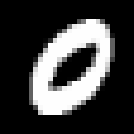
\includegraphics[interpolate=true,width=1.340000in,height=1.340000in]{dataset_samples-img0.png}}%
\end{pgfscope}%
\begin{pgfscope}%
\pgfpathrectangle{\pgfqpoint{1.516667in}{5.477218in}}{\pgfqpoint{1.333333in}{1.333333in}}%
\pgfusepath{clip}%
\pgfsys@transformshift{1.516667in}{5.477218in}%
\pgftext[left,bottom]{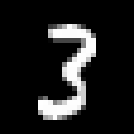
\includegraphics[interpolate=true,width=1.340000in,height=1.340000in]{dataset_samples-img1.png}}%
\end{pgfscope}%
\begin{pgfscope}%
\pgfpathrectangle{\pgfqpoint{0.050000in}{3.982228in}}{\pgfqpoint{1.333333in}{1.333333in}}%
\pgfusepath{clip}%
\pgfsys@transformshift{0.050000in}{3.982228in}%
\pgftext[left,bottom]{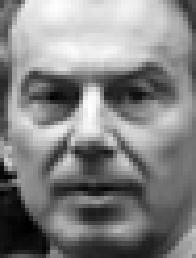
\includegraphics[interpolate=true,width=1.340000in,height=1.340000in]{dataset_samples-img2.png}}%
\end{pgfscope}%
\begin{pgfscope}%
\pgfpathrectangle{\pgfqpoint{1.516667in}{3.982228in}}{\pgfqpoint{1.333333in}{1.333333in}}%
\pgfusepath{clip}%
\pgfsys@transformshift{1.516667in}{3.982228in}%
\pgftext[left,bottom]{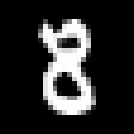
\includegraphics[interpolate=true,width=1.340000in,height=1.340000in]{dataset_samples-img3.png}}%
\end{pgfscope}%
\begin{pgfscope}%
\definecolor{textcolor}{rgb}{0.000000,0.000000,0.000000}%
\pgfsetstrokecolor{textcolor}%
\pgfsetfillcolor{textcolor}%
\pgftext[x=1.509000in,y=3.683890in,,base]{\color{textcolor}\rmfamily\fontsize{10.000000}{12.000000}\selectfont (a)}%
\end{pgfscope}%
\begin{pgfscope}%
\pgfsetbuttcap%
\pgfsetmiterjoin%
\definecolor{currentfill}{rgb}{1.000000,1.000000,1.000000}%
\pgfsetfillcolor{currentfill}%
\pgfsetlinewidth{0.000000pt}%
\definecolor{currentstroke}{rgb}{1.000000,1.000000,1.000000}%
\pgfsetstrokecolor{currentstroke}%
\pgfsetdash{}{0pt}%
\pgfpathmoveto{\pgfqpoint{-0.025000in}{0.008890in}}%
\pgfpathlineto{\pgfqpoint{2.925000in}{0.008890in}}%
\pgfpathlineto{\pgfqpoint{2.925000in}{3.508890in}}%
\pgfpathlineto{\pgfqpoint{-0.025000in}{3.508890in}}%
\pgfpathlineto{\pgfqpoint{-0.025000in}{0.008890in}}%
\pgfpathclose%
\pgfusepath{fill}%
\end{pgfscope}%
\begin{pgfscope}%
\pgfpathrectangle{\pgfqpoint{0.117792in}{1.853880in}}{\pgfqpoint{1.197749in}{1.580009in}}%
\pgfusepath{clip}%
\pgfsys@transformshift{0.117792in}{1.853880in}%
\pgftext[left,bottom]{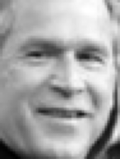
\includegraphics[interpolate=true,width=1.200000in,height=1.590000in]{dataset_samples-img4.png}}%
\end{pgfscope}%
\begin{pgfscope}%
\pgfpathrectangle{\pgfqpoint{1.584459in}{1.853880in}}{\pgfqpoint{1.197749in}{1.580009in}}%
\pgfusepath{clip}%
\pgfsys@transformshift{1.584459in}{1.853880in}%
\pgftext[left,bottom]{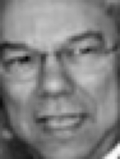
\includegraphics[interpolate=true,width=1.200000in,height=1.590000in]{dataset_samples-img5.png}}%
\end{pgfscope}%
\begin{pgfscope}%
\pgfpathrectangle{\pgfqpoint{0.117792in}{0.358890in}}{\pgfqpoint{1.197749in}{1.580009in}}%
\pgfusepath{clip}%
\pgfsys@transformshift{0.117792in}{0.358890in}%
\pgftext[left,bottom]{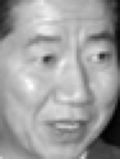
\includegraphics[interpolate=true,width=1.200000in,height=1.590000in]{dataset_samples-img6.png}}%
\end{pgfscope}%
\begin{pgfscope}%
\pgfpathrectangle{\pgfqpoint{1.584459in}{0.358890in}}{\pgfqpoint{1.197749in}{1.580009in}}%
\pgfusepath{clip}%
\pgfsys@transformshift{1.584459in}{0.358890in}%
\pgftext[left,bottom]{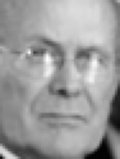
\includegraphics[interpolate=true,width=1.200000in,height=1.590000in]{dataset_samples-img7.png}}%
\end{pgfscope}%
\begin{pgfscope}%
\definecolor{textcolor}{rgb}{0.000000,0.000000,0.000000}%
\pgfsetstrokecolor{textcolor}%
\pgfsetfillcolor{textcolor}%
\pgftext[x=1.509000in,y=0.078890in,,base]{\color{textcolor}\rmfamily\fontsize{10.000000}{12.000000}\selectfont (c)}%
\end{pgfscope}%
\begin{pgfscope}%
\pgfsetbuttcap%
\pgfsetmiterjoin%
\definecolor{currentfill}{rgb}{1.000000,1.000000,1.000000}%
\pgfsetfillcolor{currentfill}%
\pgfsetlinewidth{0.000000pt}%
\definecolor{currentstroke}{rgb}{1.000000,1.000000,1.000000}%
\pgfsetstrokecolor{currentstroke}%
\pgfsetdash{}{0pt}%
\pgfpathmoveto{\pgfqpoint{2.925000in}{3.508890in}}%
\pgfpathlineto{\pgfqpoint{5.875000in}{3.508890in}}%
\pgfpathlineto{\pgfqpoint{5.875000in}{7.008890in}}%
\pgfpathlineto{\pgfqpoint{2.925000in}{7.008890in}}%
\pgfpathlineto{\pgfqpoint{2.925000in}{3.508890in}}%
\pgfpathclose%
\pgfusepath{fill}%
\end{pgfscope}%
\begin{pgfscope}%
\pgfpathrectangle{\pgfqpoint{3.000000in}{5.477218in}}{\pgfqpoint{1.333333in}{1.333333in}}%
\pgfusepath{clip}%
\pgfsys@transformshift{3.000000in}{5.477218in}%
\pgftext[left,bottom]{
\includegraphics[interpolate=true,width=1.340000in,height=1.340000in]{dataset_samples-img8.png}}%
\end{pgfscope}%
\begin{pgfscope}%
\pgfpathrectangle{\pgfqpoint{4.466667in}{5.477218in}}{\pgfqpoint{1.333333in}{1.333333in}}%
\pgfusepath{clip}%
\pgfsys@transformshift{4.466667in}{5.477218in}%
\pgftext[left,bottom]{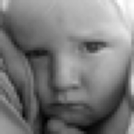
\includegraphics[interpolate=true,width=1.340000in,height=1.340000in]{dataset_samples-img9.png}}%
\end{pgfscope}%
\begin{pgfscope}%
\pgfpathrectangle{\pgfqpoint{3.000000in}{3.982228in}}{\pgfqpoint{1.333333in}{1.333333in}}%
\pgfusepath{clip}%
\pgfsys@transformshift{3.000000in}{3.982228in}%
\pgftext[left,bottom]{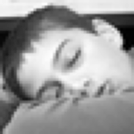
\includegraphics[interpolate=true,width=1.340000in,height=1.340000in]{dataset_samples-img10.png}}%
\end{pgfscope}%
\begin{pgfscope}%
\pgfpathrectangle{\pgfqpoint{4.466667in}{3.982228in}}{\pgfqpoint{1.333333in}{1.333333in}}%
\pgfusepath{clip}%
\pgfsys@transformshift{4.466667in}{3.982228in}%
\pgftext[left,bottom]{
\includegraphics[interpolate=true,width=1.340000in,height=1.340000in]{dataset_samples-img11.png}}%
\end{pgfscope}%
\begin{pgfscope}%
\definecolor{textcolor}{rgb}{0.000000,0.000000,0.000000}%
\pgfsetstrokecolor{textcolor}%
\pgfsetfillcolor{textcolor}%
\pgftext[x=4.459000in,y=3.683890in,,base]{\color{textcolor}\rmfamily\fontsize{10.000000}{12.000000}\selectfont (b)}%
\end{pgfscope}%
\begin{pgfscope}%
\pgfsetbuttcap%
\pgfsetmiterjoin%
\definecolor{currentfill}{rgb}{1.000000,1.000000,1.000000}%
\pgfsetfillcolor{currentfill}%
\pgfsetlinewidth{0.000000pt}%
\definecolor{currentstroke}{rgb}{1.000000,1.000000,1.000000}%
\pgfsetstrokecolor{currentstroke}%
\pgfsetdash{}{0pt}%
\pgfpathmoveto{\pgfqpoint{2.925000in}{0.008890in}}%
\pgfpathlineto{\pgfqpoint{5.875000in}{0.008890in}}%
\pgfpathlineto{\pgfqpoint{5.875000in}{3.508890in}}%
\pgfpathlineto{\pgfqpoint{2.925000in}{3.508890in}}%
\pgfpathlineto{\pgfqpoint{2.925000in}{0.008890in}}%
\pgfpathclose%
\pgfusepath{fill}%
\end{pgfscope}%
\begin{pgfscope}%
\pgfpathrectangle{\pgfqpoint{3.000000in}{1.977218in}}{\pgfqpoint{1.333333in}{1.333333in}}%
\pgfusepath{clip}%
\pgfsys@transformshift{3.000000in}{1.977218in}%
\pgftext[left,bottom]{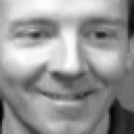
\includegraphics[interpolate=true,width=1.340000in,height=1.340000in]{dataset_samples-img12.png}}%
\end{pgfscope}%
\begin{pgfscope}%
\pgfpathrectangle{\pgfqpoint{4.466667in}{1.977218in}}{\pgfqpoint{1.333333in}{1.333333in}}%
\pgfusepath{clip}%
\pgfsys@transformshift{4.466667in}{1.977218in}%
\pgftext[left,bottom]{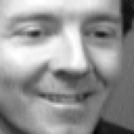
\includegraphics[interpolate=true,width=1.340000in,height=1.340000in]{dataset_samples-img13.png}}%
\end{pgfscope}%
\begin{pgfscope}%
\pgfpathrectangle{\pgfqpoint{3.000000in}{0.482228in}}{\pgfqpoint{1.333333in}{1.333333in}}%
\pgfusepath{clip}%
\pgfsys@transformshift{3.000000in}{0.482228in}%
\pgftext[left,bottom]{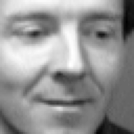
\includegraphics[interpolate=true,width=1.340000in,height=1.340000in]{dataset_samples-img14.png}}%
\end{pgfscope}%
\begin{pgfscope}%
\pgfpathrectangle{\pgfqpoint{4.466667in}{0.482228in}}{\pgfqpoint{1.333333in}{1.333333in}}%
\pgfusepath{clip}%
\pgfsys@transformshift{4.466667in}{0.482228in}%
\pgftext[left,bottom]{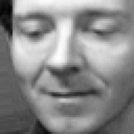
\includegraphics[interpolate=true,width=1.340000in,height=1.340000in]{dataset_samples-img15.png}}%
\end{pgfscope}%
\begin{pgfscope}%
\definecolor{textcolor}{rgb}{0.000000,0.000000,0.000000}%
\pgfsetstrokecolor{textcolor}%
\pgfsetfillcolor{textcolor}%
\pgftext[x=4.459000in,y=0.078890in,,base]{\color{textcolor}\rmfamily\fontsize{10.000000}{12.000000}\selectfont (d)}%
\end{pgfscope}%
\end{pgfpicture}%
\makeatother%
\endgroup%

	\end{center}
	\caption{Beispielbilder der natürlichen Datensätze}
	\label{fig:Dataset_samples}
\end{figure}

Letztlich ist der ICMR-Datensatz ein Gen-Datensatzs \rewrite{ICMR beschreiben}

\begin{table}[]
	\centering
	\begin{tabular}{@{}cccc@{}}
		\toprule
		Datensatz      & extrinsische Dimension $D$ & intrinsische Dimension $d$ & Stichprobengröße $n$ \\ \midrule
		Swiss Roll     & 3                          & 2                          & 5000                 \\
		Twin Peaks     & 3                          & 2                          & 5000                 \\
		MNIST          & 784                        & 10                         & 60000                \\
		Olivetti Faces & 4096                       & ?                          & 400                  \\
		LFW-People     & 2914                       & ?                          & 2370                 \\
		FER-2013       & ?                          & ?                          & ?                    \\
		ICMR           & ?                          & ?                          & ?                    \\
		\bottomrule
	\end{tabular}
	\caption{Übersicht über die Dimensionen und Stichprobengröße der verwendeten Datensätze}
	\label{tab:uebersicht-datensaetze}
\end{table}

\section{Parameterwahl und Autoencoder Architektur}
\label{ch:Vergleich:sec:ParameterwahlArchitektur}

\section{Resultate}
\label{ch:Vergleich:sec:Resultate}

In diesem Abschnitt werden die Resultate des empirischen Vergleichs vorgestellt. Dazu werden die
Werte der verschiedenen Qualitätskriterien auf den künstlichen und natürlichen Datensätzen in
Abhängigkeit der Nachbarschaftsgröße $K$ abgebildet. In
\secref{ch:Vergleich:sec:Resultate:kuenstlich} werden die Ergebnisse auf künstlichen Datensätzen
und in \secref{ch:Vergleich:sec:Resultate:natuerlich} die Ergebnisse auf den natürlichen
Datensätzen diskutiert.

\subsection{Resultate auf künstlichen Datensätzen}
\label{ch:Vergleich:sec:Resultate:kuenstlich}

Wie in \figref{fig:SwissRollMetrics}
\begin{figure}[ht]
	\begin{center}
		%% Creator: Matplotlib, PGF backend
%%
%% To include the figure in your LaTeX document, write
%%   \input{<filename>.pgf}
%%
%% Make sure the required packages are loaded in your preamble
%%   \usepackage{pgf}
%%
%% Also ensure that all the required font packages are loaded; for instance,
%% the lmodern package is sometimes necessary when using math font.
%%   \usepackage{lmodern}
%%
%% Figures using additional raster images can only be included by \input if
%% they are in the same directory as the main LaTeX file. For loading figures
%% from other directories you can use the `import` package
%%   \usepackage{import}
%%
%% and then include the figures with
%%   \import{<path to file>}{<filename>.pgf}
%%
%% Matplotlib used the following preamble
%%   
%%   \usepackage{fontspec}
%%   \setmainfont{DejaVuSerif.ttf}[Path=\detokenize{/Users/moritzmistol/.pyenv/versions/3.9.13/envs/thesis/lib/python3.9/site-packages/matplotlib/mpl-data/fonts/ttf/}]
%%   \setsansfont{DejaVuSans.ttf}[Path=\detokenize{/Users/moritzmistol/.pyenv/versions/3.9.13/envs/thesis/lib/python3.9/site-packages/matplotlib/mpl-data/fonts/ttf/}]
%%   \setmonofont{DejaVuSansMono.ttf}[Path=\detokenize{/Users/moritzmistol/.pyenv/versions/3.9.13/envs/thesis/lib/python3.9/site-packages/matplotlib/mpl-data/fonts/ttf/}]
%%   \makeatletter\@ifpackageloaded{underscore}{}{\usepackage[strings]{underscore}}\makeatother
%%
\begingroup%
\makeatletter%
\begin{pgfpicture}%
\pgfpathrectangle{\pgfpointorigin}{\pgfqpoint{5.642256in}{4.634154in}}%
\pgfusepath{use as bounding box, clip}%
\begin{pgfscope}%
\pgfsetbuttcap%
\pgfsetmiterjoin%
\definecolor{currentfill}{rgb}{1.000000,1.000000,1.000000}%
\pgfsetfillcolor{currentfill}%
\pgfsetlinewidth{0.000000pt}%
\definecolor{currentstroke}{rgb}{1.000000,1.000000,1.000000}%
\pgfsetstrokecolor{currentstroke}%
\pgfsetdash{}{0pt}%
\pgfpathmoveto{\pgfqpoint{0.000000in}{-0.000000in}}%
\pgfpathlineto{\pgfqpoint{5.642256in}{-0.000000in}}%
\pgfpathlineto{\pgfqpoint{5.642256in}{4.634154in}}%
\pgfpathlineto{\pgfqpoint{0.000000in}{4.634154in}}%
\pgfpathlineto{\pgfqpoint{0.000000in}{-0.000000in}}%
\pgfpathclose%
\pgfusepath{fill}%
\end{pgfscope}%
\begin{pgfscope}%
\pgfsetbuttcap%
\pgfsetmiterjoin%
\definecolor{currentfill}{rgb}{1.000000,1.000000,1.000000}%
\pgfsetfillcolor{currentfill}%
\pgfsetlinewidth{0.000000pt}%
\definecolor{currentstroke}{rgb}{0.000000,0.000000,0.000000}%
\pgfsetstrokecolor{currentstroke}%
\pgfsetstrokeopacity{0.000000}%
\pgfsetdash{}{0pt}%
\pgfpathmoveto{\pgfqpoint{0.539970in}{2.747992in}}%
\pgfpathlineto{\pgfqpoint{2.781441in}{2.747992in}}%
\pgfpathlineto{\pgfqpoint{2.781441in}{4.374193in}}%
\pgfpathlineto{\pgfqpoint{0.539970in}{4.374193in}}%
\pgfpathlineto{\pgfqpoint{0.539970in}{2.747992in}}%
\pgfpathclose%
\pgfusepath{fill}%
\end{pgfscope}%
\begin{pgfscope}%
\pgfsetbuttcap%
\pgfsetroundjoin%
\definecolor{currentfill}{rgb}{0.000000,0.000000,0.000000}%
\pgfsetfillcolor{currentfill}%
\pgfsetlinewidth{0.501875pt}%
\definecolor{currentstroke}{rgb}{0.000000,0.000000,0.000000}%
\pgfsetstrokecolor{currentstroke}%
\pgfsetdash{}{0pt}%
\pgfsys@defobject{currentmarker}{\pgfqpoint{0.000000in}{0.000000in}}{\pgfqpoint{0.000000in}{0.041667in}}{%
\pgfpathmoveto{\pgfqpoint{0.000000in}{0.000000in}}%
\pgfpathlineto{\pgfqpoint{0.000000in}{0.041667in}}%
\pgfusepath{stroke,fill}%
}%
\begin{pgfscope}%
\pgfsys@transformshift{0.539970in}{2.747992in}%
\pgfsys@useobject{currentmarker}{}%
\end{pgfscope}%
\end{pgfscope}%
\begin{pgfscope}%
\pgfsetbuttcap%
\pgfsetroundjoin%
\definecolor{currentfill}{rgb}{0.000000,0.000000,0.000000}%
\pgfsetfillcolor{currentfill}%
\pgfsetlinewidth{0.501875pt}%
\definecolor{currentstroke}{rgb}{0.000000,0.000000,0.000000}%
\pgfsetstrokecolor{currentstroke}%
\pgfsetdash{}{0pt}%
\pgfsys@defobject{currentmarker}{\pgfqpoint{0.000000in}{-0.041667in}}{\pgfqpoint{0.000000in}{0.000000in}}{%
\pgfpathmoveto{\pgfqpoint{0.000000in}{0.000000in}}%
\pgfpathlineto{\pgfqpoint{0.000000in}{-0.041667in}}%
\pgfusepath{stroke,fill}%
}%
\begin{pgfscope}%
\pgfsys@transformshift{0.539970in}{4.374193in}%
\pgfsys@useobject{currentmarker}{}%
\end{pgfscope}%
\end{pgfscope}%
\begin{pgfscope}%
\definecolor{textcolor}{rgb}{0.000000,0.000000,0.000000}%
\pgfsetstrokecolor{textcolor}%
\pgfsetfillcolor{textcolor}%
\pgftext[x=0.539970in,y=2.699381in,,top]{\color{textcolor}\rmfamily\fontsize{10.000000}{12.000000}\selectfont \(\displaystyle {0}\)}%
\end{pgfscope}%
\begin{pgfscope}%
\pgfsetbuttcap%
\pgfsetroundjoin%
\definecolor{currentfill}{rgb}{0.000000,0.000000,0.000000}%
\pgfsetfillcolor{currentfill}%
\pgfsetlinewidth{0.501875pt}%
\definecolor{currentstroke}{rgb}{0.000000,0.000000,0.000000}%
\pgfsetstrokecolor{currentstroke}%
\pgfsetdash{}{0pt}%
\pgfsys@defobject{currentmarker}{\pgfqpoint{0.000000in}{0.000000in}}{\pgfqpoint{0.000000in}{0.041667in}}{%
\pgfpathmoveto{\pgfqpoint{0.000000in}{0.000000in}}%
\pgfpathlineto{\pgfqpoint{0.000000in}{0.041667in}}%
\pgfusepath{stroke,fill}%
}%
\begin{pgfscope}%
\pgfsys@transformshift{0.983826in}{2.747992in}%
\pgfsys@useobject{currentmarker}{}%
\end{pgfscope}%
\end{pgfscope}%
\begin{pgfscope}%
\pgfsetbuttcap%
\pgfsetroundjoin%
\definecolor{currentfill}{rgb}{0.000000,0.000000,0.000000}%
\pgfsetfillcolor{currentfill}%
\pgfsetlinewidth{0.501875pt}%
\definecolor{currentstroke}{rgb}{0.000000,0.000000,0.000000}%
\pgfsetstrokecolor{currentstroke}%
\pgfsetdash{}{0pt}%
\pgfsys@defobject{currentmarker}{\pgfqpoint{0.000000in}{-0.041667in}}{\pgfqpoint{0.000000in}{0.000000in}}{%
\pgfpathmoveto{\pgfqpoint{0.000000in}{0.000000in}}%
\pgfpathlineto{\pgfqpoint{0.000000in}{-0.041667in}}%
\pgfusepath{stroke,fill}%
}%
\begin{pgfscope}%
\pgfsys@transformshift{0.983826in}{4.374193in}%
\pgfsys@useobject{currentmarker}{}%
\end{pgfscope}%
\end{pgfscope}%
\begin{pgfscope}%
\definecolor{textcolor}{rgb}{0.000000,0.000000,0.000000}%
\pgfsetstrokecolor{textcolor}%
\pgfsetfillcolor{textcolor}%
\pgftext[x=0.983826in,y=2.699381in,,top]{\color{textcolor}\rmfamily\fontsize{10.000000}{12.000000}\selectfont \(\displaystyle {20}\)}%
\end{pgfscope}%
\begin{pgfscope}%
\pgfsetbuttcap%
\pgfsetroundjoin%
\definecolor{currentfill}{rgb}{0.000000,0.000000,0.000000}%
\pgfsetfillcolor{currentfill}%
\pgfsetlinewidth{0.501875pt}%
\definecolor{currentstroke}{rgb}{0.000000,0.000000,0.000000}%
\pgfsetstrokecolor{currentstroke}%
\pgfsetdash{}{0pt}%
\pgfsys@defobject{currentmarker}{\pgfqpoint{0.000000in}{0.000000in}}{\pgfqpoint{0.000000in}{0.041667in}}{%
\pgfpathmoveto{\pgfqpoint{0.000000in}{0.000000in}}%
\pgfpathlineto{\pgfqpoint{0.000000in}{0.041667in}}%
\pgfusepath{stroke,fill}%
}%
\begin{pgfscope}%
\pgfsys@transformshift{1.427681in}{2.747992in}%
\pgfsys@useobject{currentmarker}{}%
\end{pgfscope}%
\end{pgfscope}%
\begin{pgfscope}%
\pgfsetbuttcap%
\pgfsetroundjoin%
\definecolor{currentfill}{rgb}{0.000000,0.000000,0.000000}%
\pgfsetfillcolor{currentfill}%
\pgfsetlinewidth{0.501875pt}%
\definecolor{currentstroke}{rgb}{0.000000,0.000000,0.000000}%
\pgfsetstrokecolor{currentstroke}%
\pgfsetdash{}{0pt}%
\pgfsys@defobject{currentmarker}{\pgfqpoint{0.000000in}{-0.041667in}}{\pgfqpoint{0.000000in}{0.000000in}}{%
\pgfpathmoveto{\pgfqpoint{0.000000in}{0.000000in}}%
\pgfpathlineto{\pgfqpoint{0.000000in}{-0.041667in}}%
\pgfusepath{stroke,fill}%
}%
\begin{pgfscope}%
\pgfsys@transformshift{1.427681in}{4.374193in}%
\pgfsys@useobject{currentmarker}{}%
\end{pgfscope}%
\end{pgfscope}%
\begin{pgfscope}%
\definecolor{textcolor}{rgb}{0.000000,0.000000,0.000000}%
\pgfsetstrokecolor{textcolor}%
\pgfsetfillcolor{textcolor}%
\pgftext[x=1.427681in,y=2.699381in,,top]{\color{textcolor}\rmfamily\fontsize{10.000000}{12.000000}\selectfont \(\displaystyle {40}\)}%
\end{pgfscope}%
\begin{pgfscope}%
\pgfsetbuttcap%
\pgfsetroundjoin%
\definecolor{currentfill}{rgb}{0.000000,0.000000,0.000000}%
\pgfsetfillcolor{currentfill}%
\pgfsetlinewidth{0.501875pt}%
\definecolor{currentstroke}{rgb}{0.000000,0.000000,0.000000}%
\pgfsetstrokecolor{currentstroke}%
\pgfsetdash{}{0pt}%
\pgfsys@defobject{currentmarker}{\pgfqpoint{0.000000in}{0.000000in}}{\pgfqpoint{0.000000in}{0.041667in}}{%
\pgfpathmoveto{\pgfqpoint{0.000000in}{0.000000in}}%
\pgfpathlineto{\pgfqpoint{0.000000in}{0.041667in}}%
\pgfusepath{stroke,fill}%
}%
\begin{pgfscope}%
\pgfsys@transformshift{1.871537in}{2.747992in}%
\pgfsys@useobject{currentmarker}{}%
\end{pgfscope}%
\end{pgfscope}%
\begin{pgfscope}%
\pgfsetbuttcap%
\pgfsetroundjoin%
\definecolor{currentfill}{rgb}{0.000000,0.000000,0.000000}%
\pgfsetfillcolor{currentfill}%
\pgfsetlinewidth{0.501875pt}%
\definecolor{currentstroke}{rgb}{0.000000,0.000000,0.000000}%
\pgfsetstrokecolor{currentstroke}%
\pgfsetdash{}{0pt}%
\pgfsys@defobject{currentmarker}{\pgfqpoint{0.000000in}{-0.041667in}}{\pgfqpoint{0.000000in}{0.000000in}}{%
\pgfpathmoveto{\pgfqpoint{0.000000in}{0.000000in}}%
\pgfpathlineto{\pgfqpoint{0.000000in}{-0.041667in}}%
\pgfusepath{stroke,fill}%
}%
\begin{pgfscope}%
\pgfsys@transformshift{1.871537in}{4.374193in}%
\pgfsys@useobject{currentmarker}{}%
\end{pgfscope}%
\end{pgfscope}%
\begin{pgfscope}%
\definecolor{textcolor}{rgb}{0.000000,0.000000,0.000000}%
\pgfsetstrokecolor{textcolor}%
\pgfsetfillcolor{textcolor}%
\pgftext[x=1.871537in,y=2.699381in,,top]{\color{textcolor}\rmfamily\fontsize{10.000000}{12.000000}\selectfont \(\displaystyle {60}\)}%
\end{pgfscope}%
\begin{pgfscope}%
\pgfsetbuttcap%
\pgfsetroundjoin%
\definecolor{currentfill}{rgb}{0.000000,0.000000,0.000000}%
\pgfsetfillcolor{currentfill}%
\pgfsetlinewidth{0.501875pt}%
\definecolor{currentstroke}{rgb}{0.000000,0.000000,0.000000}%
\pgfsetstrokecolor{currentstroke}%
\pgfsetdash{}{0pt}%
\pgfsys@defobject{currentmarker}{\pgfqpoint{0.000000in}{0.000000in}}{\pgfqpoint{0.000000in}{0.041667in}}{%
\pgfpathmoveto{\pgfqpoint{0.000000in}{0.000000in}}%
\pgfpathlineto{\pgfqpoint{0.000000in}{0.041667in}}%
\pgfusepath{stroke,fill}%
}%
\begin{pgfscope}%
\pgfsys@transformshift{2.315393in}{2.747992in}%
\pgfsys@useobject{currentmarker}{}%
\end{pgfscope}%
\end{pgfscope}%
\begin{pgfscope}%
\pgfsetbuttcap%
\pgfsetroundjoin%
\definecolor{currentfill}{rgb}{0.000000,0.000000,0.000000}%
\pgfsetfillcolor{currentfill}%
\pgfsetlinewidth{0.501875pt}%
\definecolor{currentstroke}{rgb}{0.000000,0.000000,0.000000}%
\pgfsetstrokecolor{currentstroke}%
\pgfsetdash{}{0pt}%
\pgfsys@defobject{currentmarker}{\pgfqpoint{0.000000in}{-0.041667in}}{\pgfqpoint{0.000000in}{0.000000in}}{%
\pgfpathmoveto{\pgfqpoint{0.000000in}{0.000000in}}%
\pgfpathlineto{\pgfqpoint{0.000000in}{-0.041667in}}%
\pgfusepath{stroke,fill}%
}%
\begin{pgfscope}%
\pgfsys@transformshift{2.315393in}{4.374193in}%
\pgfsys@useobject{currentmarker}{}%
\end{pgfscope}%
\end{pgfscope}%
\begin{pgfscope}%
\definecolor{textcolor}{rgb}{0.000000,0.000000,0.000000}%
\pgfsetstrokecolor{textcolor}%
\pgfsetfillcolor{textcolor}%
\pgftext[x=2.315393in,y=2.699381in,,top]{\color{textcolor}\rmfamily\fontsize{10.000000}{12.000000}\selectfont \(\displaystyle {80}\)}%
\end{pgfscope}%
\begin{pgfscope}%
\pgfsetbuttcap%
\pgfsetroundjoin%
\definecolor{currentfill}{rgb}{0.000000,0.000000,0.000000}%
\pgfsetfillcolor{currentfill}%
\pgfsetlinewidth{0.501875pt}%
\definecolor{currentstroke}{rgb}{0.000000,0.000000,0.000000}%
\pgfsetstrokecolor{currentstroke}%
\pgfsetdash{}{0pt}%
\pgfsys@defobject{currentmarker}{\pgfqpoint{0.000000in}{0.000000in}}{\pgfqpoint{0.000000in}{0.020833in}}{%
\pgfpathmoveto{\pgfqpoint{0.000000in}{0.000000in}}%
\pgfpathlineto{\pgfqpoint{0.000000in}{0.020833in}}%
\pgfusepath{stroke,fill}%
}%
\begin{pgfscope}%
\pgfsys@transformshift{0.650934in}{2.747992in}%
\pgfsys@useobject{currentmarker}{}%
\end{pgfscope}%
\end{pgfscope}%
\begin{pgfscope}%
\pgfsetbuttcap%
\pgfsetroundjoin%
\definecolor{currentfill}{rgb}{0.000000,0.000000,0.000000}%
\pgfsetfillcolor{currentfill}%
\pgfsetlinewidth{0.501875pt}%
\definecolor{currentstroke}{rgb}{0.000000,0.000000,0.000000}%
\pgfsetstrokecolor{currentstroke}%
\pgfsetdash{}{0pt}%
\pgfsys@defobject{currentmarker}{\pgfqpoint{0.000000in}{-0.020833in}}{\pgfqpoint{0.000000in}{0.000000in}}{%
\pgfpathmoveto{\pgfqpoint{0.000000in}{0.000000in}}%
\pgfpathlineto{\pgfqpoint{0.000000in}{-0.020833in}}%
\pgfusepath{stroke,fill}%
}%
\begin{pgfscope}%
\pgfsys@transformshift{0.650934in}{4.374193in}%
\pgfsys@useobject{currentmarker}{}%
\end{pgfscope}%
\end{pgfscope}%
\begin{pgfscope}%
\pgfsetbuttcap%
\pgfsetroundjoin%
\definecolor{currentfill}{rgb}{0.000000,0.000000,0.000000}%
\pgfsetfillcolor{currentfill}%
\pgfsetlinewidth{0.501875pt}%
\definecolor{currentstroke}{rgb}{0.000000,0.000000,0.000000}%
\pgfsetstrokecolor{currentstroke}%
\pgfsetdash{}{0pt}%
\pgfsys@defobject{currentmarker}{\pgfqpoint{0.000000in}{0.000000in}}{\pgfqpoint{0.000000in}{0.020833in}}{%
\pgfpathmoveto{\pgfqpoint{0.000000in}{0.000000in}}%
\pgfpathlineto{\pgfqpoint{0.000000in}{0.020833in}}%
\pgfusepath{stroke,fill}%
}%
\begin{pgfscope}%
\pgfsys@transformshift{0.761898in}{2.747992in}%
\pgfsys@useobject{currentmarker}{}%
\end{pgfscope}%
\end{pgfscope}%
\begin{pgfscope}%
\pgfsetbuttcap%
\pgfsetroundjoin%
\definecolor{currentfill}{rgb}{0.000000,0.000000,0.000000}%
\pgfsetfillcolor{currentfill}%
\pgfsetlinewidth{0.501875pt}%
\definecolor{currentstroke}{rgb}{0.000000,0.000000,0.000000}%
\pgfsetstrokecolor{currentstroke}%
\pgfsetdash{}{0pt}%
\pgfsys@defobject{currentmarker}{\pgfqpoint{0.000000in}{-0.020833in}}{\pgfqpoint{0.000000in}{0.000000in}}{%
\pgfpathmoveto{\pgfqpoint{0.000000in}{0.000000in}}%
\pgfpathlineto{\pgfqpoint{0.000000in}{-0.020833in}}%
\pgfusepath{stroke,fill}%
}%
\begin{pgfscope}%
\pgfsys@transformshift{0.761898in}{4.374193in}%
\pgfsys@useobject{currentmarker}{}%
\end{pgfscope}%
\end{pgfscope}%
\begin{pgfscope}%
\pgfsetbuttcap%
\pgfsetroundjoin%
\definecolor{currentfill}{rgb}{0.000000,0.000000,0.000000}%
\pgfsetfillcolor{currentfill}%
\pgfsetlinewidth{0.501875pt}%
\definecolor{currentstroke}{rgb}{0.000000,0.000000,0.000000}%
\pgfsetstrokecolor{currentstroke}%
\pgfsetdash{}{0pt}%
\pgfsys@defobject{currentmarker}{\pgfqpoint{0.000000in}{0.000000in}}{\pgfqpoint{0.000000in}{0.020833in}}{%
\pgfpathmoveto{\pgfqpoint{0.000000in}{0.000000in}}%
\pgfpathlineto{\pgfqpoint{0.000000in}{0.020833in}}%
\pgfusepath{stroke,fill}%
}%
\begin{pgfscope}%
\pgfsys@transformshift{0.872862in}{2.747992in}%
\pgfsys@useobject{currentmarker}{}%
\end{pgfscope}%
\end{pgfscope}%
\begin{pgfscope}%
\pgfsetbuttcap%
\pgfsetroundjoin%
\definecolor{currentfill}{rgb}{0.000000,0.000000,0.000000}%
\pgfsetfillcolor{currentfill}%
\pgfsetlinewidth{0.501875pt}%
\definecolor{currentstroke}{rgb}{0.000000,0.000000,0.000000}%
\pgfsetstrokecolor{currentstroke}%
\pgfsetdash{}{0pt}%
\pgfsys@defobject{currentmarker}{\pgfqpoint{0.000000in}{-0.020833in}}{\pgfqpoint{0.000000in}{0.000000in}}{%
\pgfpathmoveto{\pgfqpoint{0.000000in}{0.000000in}}%
\pgfpathlineto{\pgfqpoint{0.000000in}{-0.020833in}}%
\pgfusepath{stroke,fill}%
}%
\begin{pgfscope}%
\pgfsys@transformshift{0.872862in}{4.374193in}%
\pgfsys@useobject{currentmarker}{}%
\end{pgfscope}%
\end{pgfscope}%
\begin{pgfscope}%
\pgfsetbuttcap%
\pgfsetroundjoin%
\definecolor{currentfill}{rgb}{0.000000,0.000000,0.000000}%
\pgfsetfillcolor{currentfill}%
\pgfsetlinewidth{0.501875pt}%
\definecolor{currentstroke}{rgb}{0.000000,0.000000,0.000000}%
\pgfsetstrokecolor{currentstroke}%
\pgfsetdash{}{0pt}%
\pgfsys@defobject{currentmarker}{\pgfqpoint{0.000000in}{0.000000in}}{\pgfqpoint{0.000000in}{0.020833in}}{%
\pgfpathmoveto{\pgfqpoint{0.000000in}{0.000000in}}%
\pgfpathlineto{\pgfqpoint{0.000000in}{0.020833in}}%
\pgfusepath{stroke,fill}%
}%
\begin{pgfscope}%
\pgfsys@transformshift{1.094790in}{2.747992in}%
\pgfsys@useobject{currentmarker}{}%
\end{pgfscope}%
\end{pgfscope}%
\begin{pgfscope}%
\pgfsetbuttcap%
\pgfsetroundjoin%
\definecolor{currentfill}{rgb}{0.000000,0.000000,0.000000}%
\pgfsetfillcolor{currentfill}%
\pgfsetlinewidth{0.501875pt}%
\definecolor{currentstroke}{rgb}{0.000000,0.000000,0.000000}%
\pgfsetstrokecolor{currentstroke}%
\pgfsetdash{}{0pt}%
\pgfsys@defobject{currentmarker}{\pgfqpoint{0.000000in}{-0.020833in}}{\pgfqpoint{0.000000in}{0.000000in}}{%
\pgfpathmoveto{\pgfqpoint{0.000000in}{0.000000in}}%
\pgfpathlineto{\pgfqpoint{0.000000in}{-0.020833in}}%
\pgfusepath{stroke,fill}%
}%
\begin{pgfscope}%
\pgfsys@transformshift{1.094790in}{4.374193in}%
\pgfsys@useobject{currentmarker}{}%
\end{pgfscope}%
\end{pgfscope}%
\begin{pgfscope}%
\pgfsetbuttcap%
\pgfsetroundjoin%
\definecolor{currentfill}{rgb}{0.000000,0.000000,0.000000}%
\pgfsetfillcolor{currentfill}%
\pgfsetlinewidth{0.501875pt}%
\definecolor{currentstroke}{rgb}{0.000000,0.000000,0.000000}%
\pgfsetstrokecolor{currentstroke}%
\pgfsetdash{}{0pt}%
\pgfsys@defobject{currentmarker}{\pgfqpoint{0.000000in}{0.000000in}}{\pgfqpoint{0.000000in}{0.020833in}}{%
\pgfpathmoveto{\pgfqpoint{0.000000in}{0.000000in}}%
\pgfpathlineto{\pgfqpoint{0.000000in}{0.020833in}}%
\pgfusepath{stroke,fill}%
}%
\begin{pgfscope}%
\pgfsys@transformshift{1.205753in}{2.747992in}%
\pgfsys@useobject{currentmarker}{}%
\end{pgfscope}%
\end{pgfscope}%
\begin{pgfscope}%
\pgfsetbuttcap%
\pgfsetroundjoin%
\definecolor{currentfill}{rgb}{0.000000,0.000000,0.000000}%
\pgfsetfillcolor{currentfill}%
\pgfsetlinewidth{0.501875pt}%
\definecolor{currentstroke}{rgb}{0.000000,0.000000,0.000000}%
\pgfsetstrokecolor{currentstroke}%
\pgfsetdash{}{0pt}%
\pgfsys@defobject{currentmarker}{\pgfqpoint{0.000000in}{-0.020833in}}{\pgfqpoint{0.000000in}{0.000000in}}{%
\pgfpathmoveto{\pgfqpoint{0.000000in}{0.000000in}}%
\pgfpathlineto{\pgfqpoint{0.000000in}{-0.020833in}}%
\pgfusepath{stroke,fill}%
}%
\begin{pgfscope}%
\pgfsys@transformshift{1.205753in}{4.374193in}%
\pgfsys@useobject{currentmarker}{}%
\end{pgfscope}%
\end{pgfscope}%
\begin{pgfscope}%
\pgfsetbuttcap%
\pgfsetroundjoin%
\definecolor{currentfill}{rgb}{0.000000,0.000000,0.000000}%
\pgfsetfillcolor{currentfill}%
\pgfsetlinewidth{0.501875pt}%
\definecolor{currentstroke}{rgb}{0.000000,0.000000,0.000000}%
\pgfsetstrokecolor{currentstroke}%
\pgfsetdash{}{0pt}%
\pgfsys@defobject{currentmarker}{\pgfqpoint{0.000000in}{0.000000in}}{\pgfqpoint{0.000000in}{0.020833in}}{%
\pgfpathmoveto{\pgfqpoint{0.000000in}{0.000000in}}%
\pgfpathlineto{\pgfqpoint{0.000000in}{0.020833in}}%
\pgfusepath{stroke,fill}%
}%
\begin{pgfscope}%
\pgfsys@transformshift{1.316717in}{2.747992in}%
\pgfsys@useobject{currentmarker}{}%
\end{pgfscope}%
\end{pgfscope}%
\begin{pgfscope}%
\pgfsetbuttcap%
\pgfsetroundjoin%
\definecolor{currentfill}{rgb}{0.000000,0.000000,0.000000}%
\pgfsetfillcolor{currentfill}%
\pgfsetlinewidth{0.501875pt}%
\definecolor{currentstroke}{rgb}{0.000000,0.000000,0.000000}%
\pgfsetstrokecolor{currentstroke}%
\pgfsetdash{}{0pt}%
\pgfsys@defobject{currentmarker}{\pgfqpoint{0.000000in}{-0.020833in}}{\pgfqpoint{0.000000in}{0.000000in}}{%
\pgfpathmoveto{\pgfqpoint{0.000000in}{0.000000in}}%
\pgfpathlineto{\pgfqpoint{0.000000in}{-0.020833in}}%
\pgfusepath{stroke,fill}%
}%
\begin{pgfscope}%
\pgfsys@transformshift{1.316717in}{4.374193in}%
\pgfsys@useobject{currentmarker}{}%
\end{pgfscope}%
\end{pgfscope}%
\begin{pgfscope}%
\pgfsetbuttcap%
\pgfsetroundjoin%
\definecolor{currentfill}{rgb}{0.000000,0.000000,0.000000}%
\pgfsetfillcolor{currentfill}%
\pgfsetlinewidth{0.501875pt}%
\definecolor{currentstroke}{rgb}{0.000000,0.000000,0.000000}%
\pgfsetstrokecolor{currentstroke}%
\pgfsetdash{}{0pt}%
\pgfsys@defobject{currentmarker}{\pgfqpoint{0.000000in}{0.000000in}}{\pgfqpoint{0.000000in}{0.020833in}}{%
\pgfpathmoveto{\pgfqpoint{0.000000in}{0.000000in}}%
\pgfpathlineto{\pgfqpoint{0.000000in}{0.020833in}}%
\pgfusepath{stroke,fill}%
}%
\begin{pgfscope}%
\pgfsys@transformshift{1.538645in}{2.747992in}%
\pgfsys@useobject{currentmarker}{}%
\end{pgfscope}%
\end{pgfscope}%
\begin{pgfscope}%
\pgfsetbuttcap%
\pgfsetroundjoin%
\definecolor{currentfill}{rgb}{0.000000,0.000000,0.000000}%
\pgfsetfillcolor{currentfill}%
\pgfsetlinewidth{0.501875pt}%
\definecolor{currentstroke}{rgb}{0.000000,0.000000,0.000000}%
\pgfsetstrokecolor{currentstroke}%
\pgfsetdash{}{0pt}%
\pgfsys@defobject{currentmarker}{\pgfqpoint{0.000000in}{-0.020833in}}{\pgfqpoint{0.000000in}{0.000000in}}{%
\pgfpathmoveto{\pgfqpoint{0.000000in}{0.000000in}}%
\pgfpathlineto{\pgfqpoint{0.000000in}{-0.020833in}}%
\pgfusepath{stroke,fill}%
}%
\begin{pgfscope}%
\pgfsys@transformshift{1.538645in}{4.374193in}%
\pgfsys@useobject{currentmarker}{}%
\end{pgfscope}%
\end{pgfscope}%
\begin{pgfscope}%
\pgfsetbuttcap%
\pgfsetroundjoin%
\definecolor{currentfill}{rgb}{0.000000,0.000000,0.000000}%
\pgfsetfillcolor{currentfill}%
\pgfsetlinewidth{0.501875pt}%
\definecolor{currentstroke}{rgb}{0.000000,0.000000,0.000000}%
\pgfsetstrokecolor{currentstroke}%
\pgfsetdash{}{0pt}%
\pgfsys@defobject{currentmarker}{\pgfqpoint{0.000000in}{0.000000in}}{\pgfqpoint{0.000000in}{0.020833in}}{%
\pgfpathmoveto{\pgfqpoint{0.000000in}{0.000000in}}%
\pgfpathlineto{\pgfqpoint{0.000000in}{0.020833in}}%
\pgfusepath{stroke,fill}%
}%
\begin{pgfscope}%
\pgfsys@transformshift{1.649609in}{2.747992in}%
\pgfsys@useobject{currentmarker}{}%
\end{pgfscope}%
\end{pgfscope}%
\begin{pgfscope}%
\pgfsetbuttcap%
\pgfsetroundjoin%
\definecolor{currentfill}{rgb}{0.000000,0.000000,0.000000}%
\pgfsetfillcolor{currentfill}%
\pgfsetlinewidth{0.501875pt}%
\definecolor{currentstroke}{rgb}{0.000000,0.000000,0.000000}%
\pgfsetstrokecolor{currentstroke}%
\pgfsetdash{}{0pt}%
\pgfsys@defobject{currentmarker}{\pgfqpoint{0.000000in}{-0.020833in}}{\pgfqpoint{0.000000in}{0.000000in}}{%
\pgfpathmoveto{\pgfqpoint{0.000000in}{0.000000in}}%
\pgfpathlineto{\pgfqpoint{0.000000in}{-0.020833in}}%
\pgfusepath{stroke,fill}%
}%
\begin{pgfscope}%
\pgfsys@transformshift{1.649609in}{4.374193in}%
\pgfsys@useobject{currentmarker}{}%
\end{pgfscope}%
\end{pgfscope}%
\begin{pgfscope}%
\pgfsetbuttcap%
\pgfsetroundjoin%
\definecolor{currentfill}{rgb}{0.000000,0.000000,0.000000}%
\pgfsetfillcolor{currentfill}%
\pgfsetlinewidth{0.501875pt}%
\definecolor{currentstroke}{rgb}{0.000000,0.000000,0.000000}%
\pgfsetstrokecolor{currentstroke}%
\pgfsetdash{}{0pt}%
\pgfsys@defobject{currentmarker}{\pgfqpoint{0.000000in}{0.000000in}}{\pgfqpoint{0.000000in}{0.020833in}}{%
\pgfpathmoveto{\pgfqpoint{0.000000in}{0.000000in}}%
\pgfpathlineto{\pgfqpoint{0.000000in}{0.020833in}}%
\pgfusepath{stroke,fill}%
}%
\begin{pgfscope}%
\pgfsys@transformshift{1.760573in}{2.747992in}%
\pgfsys@useobject{currentmarker}{}%
\end{pgfscope}%
\end{pgfscope}%
\begin{pgfscope}%
\pgfsetbuttcap%
\pgfsetroundjoin%
\definecolor{currentfill}{rgb}{0.000000,0.000000,0.000000}%
\pgfsetfillcolor{currentfill}%
\pgfsetlinewidth{0.501875pt}%
\definecolor{currentstroke}{rgb}{0.000000,0.000000,0.000000}%
\pgfsetstrokecolor{currentstroke}%
\pgfsetdash{}{0pt}%
\pgfsys@defobject{currentmarker}{\pgfqpoint{0.000000in}{-0.020833in}}{\pgfqpoint{0.000000in}{0.000000in}}{%
\pgfpathmoveto{\pgfqpoint{0.000000in}{0.000000in}}%
\pgfpathlineto{\pgfqpoint{0.000000in}{-0.020833in}}%
\pgfusepath{stroke,fill}%
}%
\begin{pgfscope}%
\pgfsys@transformshift{1.760573in}{4.374193in}%
\pgfsys@useobject{currentmarker}{}%
\end{pgfscope}%
\end{pgfscope}%
\begin{pgfscope}%
\pgfsetbuttcap%
\pgfsetroundjoin%
\definecolor{currentfill}{rgb}{0.000000,0.000000,0.000000}%
\pgfsetfillcolor{currentfill}%
\pgfsetlinewidth{0.501875pt}%
\definecolor{currentstroke}{rgb}{0.000000,0.000000,0.000000}%
\pgfsetstrokecolor{currentstroke}%
\pgfsetdash{}{0pt}%
\pgfsys@defobject{currentmarker}{\pgfqpoint{0.000000in}{0.000000in}}{\pgfqpoint{0.000000in}{0.020833in}}{%
\pgfpathmoveto{\pgfqpoint{0.000000in}{0.000000in}}%
\pgfpathlineto{\pgfqpoint{0.000000in}{0.020833in}}%
\pgfusepath{stroke,fill}%
}%
\begin{pgfscope}%
\pgfsys@transformshift{1.982501in}{2.747992in}%
\pgfsys@useobject{currentmarker}{}%
\end{pgfscope}%
\end{pgfscope}%
\begin{pgfscope}%
\pgfsetbuttcap%
\pgfsetroundjoin%
\definecolor{currentfill}{rgb}{0.000000,0.000000,0.000000}%
\pgfsetfillcolor{currentfill}%
\pgfsetlinewidth{0.501875pt}%
\definecolor{currentstroke}{rgb}{0.000000,0.000000,0.000000}%
\pgfsetstrokecolor{currentstroke}%
\pgfsetdash{}{0pt}%
\pgfsys@defobject{currentmarker}{\pgfqpoint{0.000000in}{-0.020833in}}{\pgfqpoint{0.000000in}{0.000000in}}{%
\pgfpathmoveto{\pgfqpoint{0.000000in}{0.000000in}}%
\pgfpathlineto{\pgfqpoint{0.000000in}{-0.020833in}}%
\pgfusepath{stroke,fill}%
}%
\begin{pgfscope}%
\pgfsys@transformshift{1.982501in}{4.374193in}%
\pgfsys@useobject{currentmarker}{}%
\end{pgfscope}%
\end{pgfscope}%
\begin{pgfscope}%
\pgfsetbuttcap%
\pgfsetroundjoin%
\definecolor{currentfill}{rgb}{0.000000,0.000000,0.000000}%
\pgfsetfillcolor{currentfill}%
\pgfsetlinewidth{0.501875pt}%
\definecolor{currentstroke}{rgb}{0.000000,0.000000,0.000000}%
\pgfsetstrokecolor{currentstroke}%
\pgfsetdash{}{0pt}%
\pgfsys@defobject{currentmarker}{\pgfqpoint{0.000000in}{0.000000in}}{\pgfqpoint{0.000000in}{0.020833in}}{%
\pgfpathmoveto{\pgfqpoint{0.000000in}{0.000000in}}%
\pgfpathlineto{\pgfqpoint{0.000000in}{0.020833in}}%
\pgfusepath{stroke,fill}%
}%
\begin{pgfscope}%
\pgfsys@transformshift{2.093465in}{2.747992in}%
\pgfsys@useobject{currentmarker}{}%
\end{pgfscope}%
\end{pgfscope}%
\begin{pgfscope}%
\pgfsetbuttcap%
\pgfsetroundjoin%
\definecolor{currentfill}{rgb}{0.000000,0.000000,0.000000}%
\pgfsetfillcolor{currentfill}%
\pgfsetlinewidth{0.501875pt}%
\definecolor{currentstroke}{rgb}{0.000000,0.000000,0.000000}%
\pgfsetstrokecolor{currentstroke}%
\pgfsetdash{}{0pt}%
\pgfsys@defobject{currentmarker}{\pgfqpoint{0.000000in}{-0.020833in}}{\pgfqpoint{0.000000in}{0.000000in}}{%
\pgfpathmoveto{\pgfqpoint{0.000000in}{0.000000in}}%
\pgfpathlineto{\pgfqpoint{0.000000in}{-0.020833in}}%
\pgfusepath{stroke,fill}%
}%
\begin{pgfscope}%
\pgfsys@transformshift{2.093465in}{4.374193in}%
\pgfsys@useobject{currentmarker}{}%
\end{pgfscope}%
\end{pgfscope}%
\begin{pgfscope}%
\pgfsetbuttcap%
\pgfsetroundjoin%
\definecolor{currentfill}{rgb}{0.000000,0.000000,0.000000}%
\pgfsetfillcolor{currentfill}%
\pgfsetlinewidth{0.501875pt}%
\definecolor{currentstroke}{rgb}{0.000000,0.000000,0.000000}%
\pgfsetstrokecolor{currentstroke}%
\pgfsetdash{}{0pt}%
\pgfsys@defobject{currentmarker}{\pgfqpoint{0.000000in}{0.000000in}}{\pgfqpoint{0.000000in}{0.020833in}}{%
\pgfpathmoveto{\pgfqpoint{0.000000in}{0.000000in}}%
\pgfpathlineto{\pgfqpoint{0.000000in}{0.020833in}}%
\pgfusepath{stroke,fill}%
}%
\begin{pgfscope}%
\pgfsys@transformshift{2.204429in}{2.747992in}%
\pgfsys@useobject{currentmarker}{}%
\end{pgfscope}%
\end{pgfscope}%
\begin{pgfscope}%
\pgfsetbuttcap%
\pgfsetroundjoin%
\definecolor{currentfill}{rgb}{0.000000,0.000000,0.000000}%
\pgfsetfillcolor{currentfill}%
\pgfsetlinewidth{0.501875pt}%
\definecolor{currentstroke}{rgb}{0.000000,0.000000,0.000000}%
\pgfsetstrokecolor{currentstroke}%
\pgfsetdash{}{0pt}%
\pgfsys@defobject{currentmarker}{\pgfqpoint{0.000000in}{-0.020833in}}{\pgfqpoint{0.000000in}{0.000000in}}{%
\pgfpathmoveto{\pgfqpoint{0.000000in}{0.000000in}}%
\pgfpathlineto{\pgfqpoint{0.000000in}{-0.020833in}}%
\pgfusepath{stroke,fill}%
}%
\begin{pgfscope}%
\pgfsys@transformshift{2.204429in}{4.374193in}%
\pgfsys@useobject{currentmarker}{}%
\end{pgfscope}%
\end{pgfscope}%
\begin{pgfscope}%
\pgfsetbuttcap%
\pgfsetroundjoin%
\definecolor{currentfill}{rgb}{0.000000,0.000000,0.000000}%
\pgfsetfillcolor{currentfill}%
\pgfsetlinewidth{0.501875pt}%
\definecolor{currentstroke}{rgb}{0.000000,0.000000,0.000000}%
\pgfsetstrokecolor{currentstroke}%
\pgfsetdash{}{0pt}%
\pgfsys@defobject{currentmarker}{\pgfqpoint{0.000000in}{0.000000in}}{\pgfqpoint{0.000000in}{0.020833in}}{%
\pgfpathmoveto{\pgfqpoint{0.000000in}{0.000000in}}%
\pgfpathlineto{\pgfqpoint{0.000000in}{0.020833in}}%
\pgfusepath{stroke,fill}%
}%
\begin{pgfscope}%
\pgfsys@transformshift{2.426357in}{2.747992in}%
\pgfsys@useobject{currentmarker}{}%
\end{pgfscope}%
\end{pgfscope}%
\begin{pgfscope}%
\pgfsetbuttcap%
\pgfsetroundjoin%
\definecolor{currentfill}{rgb}{0.000000,0.000000,0.000000}%
\pgfsetfillcolor{currentfill}%
\pgfsetlinewidth{0.501875pt}%
\definecolor{currentstroke}{rgb}{0.000000,0.000000,0.000000}%
\pgfsetstrokecolor{currentstroke}%
\pgfsetdash{}{0pt}%
\pgfsys@defobject{currentmarker}{\pgfqpoint{0.000000in}{-0.020833in}}{\pgfqpoint{0.000000in}{0.000000in}}{%
\pgfpathmoveto{\pgfqpoint{0.000000in}{0.000000in}}%
\pgfpathlineto{\pgfqpoint{0.000000in}{-0.020833in}}%
\pgfusepath{stroke,fill}%
}%
\begin{pgfscope}%
\pgfsys@transformshift{2.426357in}{4.374193in}%
\pgfsys@useobject{currentmarker}{}%
\end{pgfscope}%
\end{pgfscope}%
\begin{pgfscope}%
\pgfsetbuttcap%
\pgfsetroundjoin%
\definecolor{currentfill}{rgb}{0.000000,0.000000,0.000000}%
\pgfsetfillcolor{currentfill}%
\pgfsetlinewidth{0.501875pt}%
\definecolor{currentstroke}{rgb}{0.000000,0.000000,0.000000}%
\pgfsetstrokecolor{currentstroke}%
\pgfsetdash{}{0pt}%
\pgfsys@defobject{currentmarker}{\pgfqpoint{0.000000in}{0.000000in}}{\pgfqpoint{0.000000in}{0.020833in}}{%
\pgfpathmoveto{\pgfqpoint{0.000000in}{0.000000in}}%
\pgfpathlineto{\pgfqpoint{0.000000in}{0.020833in}}%
\pgfusepath{stroke,fill}%
}%
\begin{pgfscope}%
\pgfsys@transformshift{2.537321in}{2.747992in}%
\pgfsys@useobject{currentmarker}{}%
\end{pgfscope}%
\end{pgfscope}%
\begin{pgfscope}%
\pgfsetbuttcap%
\pgfsetroundjoin%
\definecolor{currentfill}{rgb}{0.000000,0.000000,0.000000}%
\pgfsetfillcolor{currentfill}%
\pgfsetlinewidth{0.501875pt}%
\definecolor{currentstroke}{rgb}{0.000000,0.000000,0.000000}%
\pgfsetstrokecolor{currentstroke}%
\pgfsetdash{}{0pt}%
\pgfsys@defobject{currentmarker}{\pgfqpoint{0.000000in}{-0.020833in}}{\pgfqpoint{0.000000in}{0.000000in}}{%
\pgfpathmoveto{\pgfqpoint{0.000000in}{0.000000in}}%
\pgfpathlineto{\pgfqpoint{0.000000in}{-0.020833in}}%
\pgfusepath{stroke,fill}%
}%
\begin{pgfscope}%
\pgfsys@transformshift{2.537321in}{4.374193in}%
\pgfsys@useobject{currentmarker}{}%
\end{pgfscope}%
\end{pgfscope}%
\begin{pgfscope}%
\pgfsetbuttcap%
\pgfsetroundjoin%
\definecolor{currentfill}{rgb}{0.000000,0.000000,0.000000}%
\pgfsetfillcolor{currentfill}%
\pgfsetlinewidth{0.501875pt}%
\definecolor{currentstroke}{rgb}{0.000000,0.000000,0.000000}%
\pgfsetstrokecolor{currentstroke}%
\pgfsetdash{}{0pt}%
\pgfsys@defobject{currentmarker}{\pgfqpoint{0.000000in}{0.000000in}}{\pgfqpoint{0.000000in}{0.020833in}}{%
\pgfpathmoveto{\pgfqpoint{0.000000in}{0.000000in}}%
\pgfpathlineto{\pgfqpoint{0.000000in}{0.020833in}}%
\pgfusepath{stroke,fill}%
}%
\begin{pgfscope}%
\pgfsys@transformshift{2.648285in}{2.747992in}%
\pgfsys@useobject{currentmarker}{}%
\end{pgfscope}%
\end{pgfscope}%
\begin{pgfscope}%
\pgfsetbuttcap%
\pgfsetroundjoin%
\definecolor{currentfill}{rgb}{0.000000,0.000000,0.000000}%
\pgfsetfillcolor{currentfill}%
\pgfsetlinewidth{0.501875pt}%
\definecolor{currentstroke}{rgb}{0.000000,0.000000,0.000000}%
\pgfsetstrokecolor{currentstroke}%
\pgfsetdash{}{0pt}%
\pgfsys@defobject{currentmarker}{\pgfqpoint{0.000000in}{-0.020833in}}{\pgfqpoint{0.000000in}{0.000000in}}{%
\pgfpathmoveto{\pgfqpoint{0.000000in}{0.000000in}}%
\pgfpathlineto{\pgfqpoint{0.000000in}{-0.020833in}}%
\pgfusepath{stroke,fill}%
}%
\begin{pgfscope}%
\pgfsys@transformshift{2.648285in}{4.374193in}%
\pgfsys@useobject{currentmarker}{}%
\end{pgfscope}%
\end{pgfscope}%
\begin{pgfscope}%
\pgfsetbuttcap%
\pgfsetroundjoin%
\definecolor{currentfill}{rgb}{0.000000,0.000000,0.000000}%
\pgfsetfillcolor{currentfill}%
\pgfsetlinewidth{0.501875pt}%
\definecolor{currentstroke}{rgb}{0.000000,0.000000,0.000000}%
\pgfsetstrokecolor{currentstroke}%
\pgfsetdash{}{0pt}%
\pgfsys@defobject{currentmarker}{\pgfqpoint{0.000000in}{0.000000in}}{\pgfqpoint{0.000000in}{0.020833in}}{%
\pgfpathmoveto{\pgfqpoint{0.000000in}{0.000000in}}%
\pgfpathlineto{\pgfqpoint{0.000000in}{0.020833in}}%
\pgfusepath{stroke,fill}%
}%
\begin{pgfscope}%
\pgfsys@transformshift{2.759249in}{2.747992in}%
\pgfsys@useobject{currentmarker}{}%
\end{pgfscope}%
\end{pgfscope}%
\begin{pgfscope}%
\pgfsetbuttcap%
\pgfsetroundjoin%
\definecolor{currentfill}{rgb}{0.000000,0.000000,0.000000}%
\pgfsetfillcolor{currentfill}%
\pgfsetlinewidth{0.501875pt}%
\definecolor{currentstroke}{rgb}{0.000000,0.000000,0.000000}%
\pgfsetstrokecolor{currentstroke}%
\pgfsetdash{}{0pt}%
\pgfsys@defobject{currentmarker}{\pgfqpoint{0.000000in}{-0.020833in}}{\pgfqpoint{0.000000in}{0.000000in}}{%
\pgfpathmoveto{\pgfqpoint{0.000000in}{0.000000in}}%
\pgfpathlineto{\pgfqpoint{0.000000in}{-0.020833in}}%
\pgfusepath{stroke,fill}%
}%
\begin{pgfscope}%
\pgfsys@transformshift{2.759249in}{4.374193in}%
\pgfsys@useobject{currentmarker}{}%
\end{pgfscope}%
\end{pgfscope}%
\begin{pgfscope}%
\definecolor{textcolor}{rgb}{0.000000,0.000000,0.000000}%
\pgfsetstrokecolor{textcolor}%
\pgfsetfillcolor{textcolor}%
\pgftext[x=1.660706in,y=2.509413in,,top]{\color{textcolor}\rmfamily\fontsize{10.000000}{12.000000}\selectfont \(\displaystyle K\)}%
\end{pgfscope}%
\begin{pgfscope}%
\pgfsetbuttcap%
\pgfsetroundjoin%
\definecolor{currentfill}{rgb}{0.000000,0.000000,0.000000}%
\pgfsetfillcolor{currentfill}%
\pgfsetlinewidth{0.501875pt}%
\definecolor{currentstroke}{rgb}{0.000000,0.000000,0.000000}%
\pgfsetstrokecolor{currentstroke}%
\pgfsetdash{}{0pt}%
\pgfsys@defobject{currentmarker}{\pgfqpoint{0.000000in}{0.000000in}}{\pgfqpoint{0.041667in}{0.000000in}}{%
\pgfpathmoveto{\pgfqpoint{0.000000in}{0.000000in}}%
\pgfpathlineto{\pgfqpoint{0.041667in}{0.000000in}}%
\pgfusepath{stroke,fill}%
}%
\begin{pgfscope}%
\pgfsys@transformshift{0.539970in}{2.892037in}%
\pgfsys@useobject{currentmarker}{}%
\end{pgfscope}%
\end{pgfscope}%
\begin{pgfscope}%
\pgfsetbuttcap%
\pgfsetroundjoin%
\definecolor{currentfill}{rgb}{0.000000,0.000000,0.000000}%
\pgfsetfillcolor{currentfill}%
\pgfsetlinewidth{0.501875pt}%
\definecolor{currentstroke}{rgb}{0.000000,0.000000,0.000000}%
\pgfsetstrokecolor{currentstroke}%
\pgfsetdash{}{0pt}%
\pgfsys@defobject{currentmarker}{\pgfqpoint{-0.041667in}{0.000000in}}{\pgfqpoint{-0.000000in}{0.000000in}}{%
\pgfpathmoveto{\pgfqpoint{-0.000000in}{0.000000in}}%
\pgfpathlineto{\pgfqpoint{-0.041667in}{0.000000in}}%
\pgfusepath{stroke,fill}%
}%
\begin{pgfscope}%
\pgfsys@transformshift{2.781441in}{2.892037in}%
\pgfsys@useobject{currentmarker}{}%
\end{pgfscope}%
\end{pgfscope}%
\begin{pgfscope}%
\definecolor{textcolor}{rgb}{0.000000,0.000000,0.000000}%
\pgfsetstrokecolor{textcolor}%
\pgfsetfillcolor{textcolor}%
\pgftext[x=0.244444in, y=2.839276in, left, base]{\color{textcolor}\rmfamily\fontsize{10.000000}{12.000000}\selectfont \(\displaystyle {0.82}\)}%
\end{pgfscope}%
\begin{pgfscope}%
\pgfsetbuttcap%
\pgfsetroundjoin%
\definecolor{currentfill}{rgb}{0.000000,0.000000,0.000000}%
\pgfsetfillcolor{currentfill}%
\pgfsetlinewidth{0.501875pt}%
\definecolor{currentstroke}{rgb}{0.000000,0.000000,0.000000}%
\pgfsetstrokecolor{currentstroke}%
\pgfsetdash{}{0pt}%
\pgfsys@defobject{currentmarker}{\pgfqpoint{0.000000in}{0.000000in}}{\pgfqpoint{0.041667in}{0.000000in}}{%
\pgfpathmoveto{\pgfqpoint{0.000000in}{0.000000in}}%
\pgfpathlineto{\pgfqpoint{0.041667in}{0.000000in}}%
\pgfusepath{stroke,fill}%
}%
\begin{pgfscope}%
\pgfsys@transformshift{0.539970in}{3.324531in}%
\pgfsys@useobject{currentmarker}{}%
\end{pgfscope}%
\end{pgfscope}%
\begin{pgfscope}%
\pgfsetbuttcap%
\pgfsetroundjoin%
\definecolor{currentfill}{rgb}{0.000000,0.000000,0.000000}%
\pgfsetfillcolor{currentfill}%
\pgfsetlinewidth{0.501875pt}%
\definecolor{currentstroke}{rgb}{0.000000,0.000000,0.000000}%
\pgfsetstrokecolor{currentstroke}%
\pgfsetdash{}{0pt}%
\pgfsys@defobject{currentmarker}{\pgfqpoint{-0.041667in}{0.000000in}}{\pgfqpoint{-0.000000in}{0.000000in}}{%
\pgfpathmoveto{\pgfqpoint{-0.000000in}{0.000000in}}%
\pgfpathlineto{\pgfqpoint{-0.041667in}{0.000000in}}%
\pgfusepath{stroke,fill}%
}%
\begin{pgfscope}%
\pgfsys@transformshift{2.781441in}{3.324531in}%
\pgfsys@useobject{currentmarker}{}%
\end{pgfscope}%
\end{pgfscope}%
\begin{pgfscope}%
\definecolor{textcolor}{rgb}{0.000000,0.000000,0.000000}%
\pgfsetstrokecolor{textcolor}%
\pgfsetfillcolor{textcolor}%
\pgftext[x=0.244444in, y=3.271770in, left, base]{\color{textcolor}\rmfamily\fontsize{10.000000}{12.000000}\selectfont \(\displaystyle {0.84}\)}%
\end{pgfscope}%
\begin{pgfscope}%
\pgfsetbuttcap%
\pgfsetroundjoin%
\definecolor{currentfill}{rgb}{0.000000,0.000000,0.000000}%
\pgfsetfillcolor{currentfill}%
\pgfsetlinewidth{0.501875pt}%
\definecolor{currentstroke}{rgb}{0.000000,0.000000,0.000000}%
\pgfsetstrokecolor{currentstroke}%
\pgfsetdash{}{0pt}%
\pgfsys@defobject{currentmarker}{\pgfqpoint{0.000000in}{0.000000in}}{\pgfqpoint{0.041667in}{0.000000in}}{%
\pgfpathmoveto{\pgfqpoint{0.000000in}{0.000000in}}%
\pgfpathlineto{\pgfqpoint{0.041667in}{0.000000in}}%
\pgfusepath{stroke,fill}%
}%
\begin{pgfscope}%
\pgfsys@transformshift{0.539970in}{3.757025in}%
\pgfsys@useobject{currentmarker}{}%
\end{pgfscope}%
\end{pgfscope}%
\begin{pgfscope}%
\pgfsetbuttcap%
\pgfsetroundjoin%
\definecolor{currentfill}{rgb}{0.000000,0.000000,0.000000}%
\pgfsetfillcolor{currentfill}%
\pgfsetlinewidth{0.501875pt}%
\definecolor{currentstroke}{rgb}{0.000000,0.000000,0.000000}%
\pgfsetstrokecolor{currentstroke}%
\pgfsetdash{}{0pt}%
\pgfsys@defobject{currentmarker}{\pgfqpoint{-0.041667in}{0.000000in}}{\pgfqpoint{-0.000000in}{0.000000in}}{%
\pgfpathmoveto{\pgfqpoint{-0.000000in}{0.000000in}}%
\pgfpathlineto{\pgfqpoint{-0.041667in}{0.000000in}}%
\pgfusepath{stroke,fill}%
}%
\begin{pgfscope}%
\pgfsys@transformshift{2.781441in}{3.757025in}%
\pgfsys@useobject{currentmarker}{}%
\end{pgfscope}%
\end{pgfscope}%
\begin{pgfscope}%
\definecolor{textcolor}{rgb}{0.000000,0.000000,0.000000}%
\pgfsetstrokecolor{textcolor}%
\pgfsetfillcolor{textcolor}%
\pgftext[x=0.244444in, y=3.704263in, left, base]{\color{textcolor}\rmfamily\fontsize{10.000000}{12.000000}\selectfont \(\displaystyle {0.86}\)}%
\end{pgfscope}%
\begin{pgfscope}%
\pgfsetbuttcap%
\pgfsetroundjoin%
\definecolor{currentfill}{rgb}{0.000000,0.000000,0.000000}%
\pgfsetfillcolor{currentfill}%
\pgfsetlinewidth{0.501875pt}%
\definecolor{currentstroke}{rgb}{0.000000,0.000000,0.000000}%
\pgfsetstrokecolor{currentstroke}%
\pgfsetdash{}{0pt}%
\pgfsys@defobject{currentmarker}{\pgfqpoint{0.000000in}{0.000000in}}{\pgfqpoint{0.041667in}{0.000000in}}{%
\pgfpathmoveto{\pgfqpoint{0.000000in}{0.000000in}}%
\pgfpathlineto{\pgfqpoint{0.041667in}{0.000000in}}%
\pgfusepath{stroke,fill}%
}%
\begin{pgfscope}%
\pgfsys@transformshift{0.539970in}{4.189519in}%
\pgfsys@useobject{currentmarker}{}%
\end{pgfscope}%
\end{pgfscope}%
\begin{pgfscope}%
\pgfsetbuttcap%
\pgfsetroundjoin%
\definecolor{currentfill}{rgb}{0.000000,0.000000,0.000000}%
\pgfsetfillcolor{currentfill}%
\pgfsetlinewidth{0.501875pt}%
\definecolor{currentstroke}{rgb}{0.000000,0.000000,0.000000}%
\pgfsetstrokecolor{currentstroke}%
\pgfsetdash{}{0pt}%
\pgfsys@defobject{currentmarker}{\pgfqpoint{-0.041667in}{0.000000in}}{\pgfqpoint{-0.000000in}{0.000000in}}{%
\pgfpathmoveto{\pgfqpoint{-0.000000in}{0.000000in}}%
\pgfpathlineto{\pgfqpoint{-0.041667in}{0.000000in}}%
\pgfusepath{stroke,fill}%
}%
\begin{pgfscope}%
\pgfsys@transformshift{2.781441in}{4.189519in}%
\pgfsys@useobject{currentmarker}{}%
\end{pgfscope}%
\end{pgfscope}%
\begin{pgfscope}%
\definecolor{textcolor}{rgb}{0.000000,0.000000,0.000000}%
\pgfsetstrokecolor{textcolor}%
\pgfsetfillcolor{textcolor}%
\pgftext[x=0.244444in, y=4.136757in, left, base]{\color{textcolor}\rmfamily\fontsize{10.000000}{12.000000}\selectfont \(\displaystyle {0.88}\)}%
\end{pgfscope}%
\begin{pgfscope}%
\pgfsetbuttcap%
\pgfsetroundjoin%
\definecolor{currentfill}{rgb}{0.000000,0.000000,0.000000}%
\pgfsetfillcolor{currentfill}%
\pgfsetlinewidth{0.501875pt}%
\definecolor{currentstroke}{rgb}{0.000000,0.000000,0.000000}%
\pgfsetstrokecolor{currentstroke}%
\pgfsetdash{}{0pt}%
\pgfsys@defobject{currentmarker}{\pgfqpoint{0.000000in}{0.000000in}}{\pgfqpoint{0.020833in}{0.000000in}}{%
\pgfpathmoveto{\pgfqpoint{0.000000in}{0.000000in}}%
\pgfpathlineto{\pgfqpoint{0.020833in}{0.000000in}}%
\pgfusepath{stroke,fill}%
}%
\begin{pgfscope}%
\pgfsys@transformshift{0.539970in}{2.783914in}%
\pgfsys@useobject{currentmarker}{}%
\end{pgfscope}%
\end{pgfscope}%
\begin{pgfscope}%
\pgfsetbuttcap%
\pgfsetroundjoin%
\definecolor{currentfill}{rgb}{0.000000,0.000000,0.000000}%
\pgfsetfillcolor{currentfill}%
\pgfsetlinewidth{0.501875pt}%
\definecolor{currentstroke}{rgb}{0.000000,0.000000,0.000000}%
\pgfsetstrokecolor{currentstroke}%
\pgfsetdash{}{0pt}%
\pgfsys@defobject{currentmarker}{\pgfqpoint{-0.020833in}{0.000000in}}{\pgfqpoint{-0.000000in}{0.000000in}}{%
\pgfpathmoveto{\pgfqpoint{-0.000000in}{0.000000in}}%
\pgfpathlineto{\pgfqpoint{-0.020833in}{0.000000in}}%
\pgfusepath{stroke,fill}%
}%
\begin{pgfscope}%
\pgfsys@transformshift{2.781441in}{2.783914in}%
\pgfsys@useobject{currentmarker}{}%
\end{pgfscope}%
\end{pgfscope}%
\begin{pgfscope}%
\pgfsetbuttcap%
\pgfsetroundjoin%
\definecolor{currentfill}{rgb}{0.000000,0.000000,0.000000}%
\pgfsetfillcolor{currentfill}%
\pgfsetlinewidth{0.501875pt}%
\definecolor{currentstroke}{rgb}{0.000000,0.000000,0.000000}%
\pgfsetstrokecolor{currentstroke}%
\pgfsetdash{}{0pt}%
\pgfsys@defobject{currentmarker}{\pgfqpoint{0.000000in}{0.000000in}}{\pgfqpoint{0.020833in}{0.000000in}}{%
\pgfpathmoveto{\pgfqpoint{0.000000in}{0.000000in}}%
\pgfpathlineto{\pgfqpoint{0.020833in}{0.000000in}}%
\pgfusepath{stroke,fill}%
}%
\begin{pgfscope}%
\pgfsys@transformshift{0.539970in}{3.000161in}%
\pgfsys@useobject{currentmarker}{}%
\end{pgfscope}%
\end{pgfscope}%
\begin{pgfscope}%
\pgfsetbuttcap%
\pgfsetroundjoin%
\definecolor{currentfill}{rgb}{0.000000,0.000000,0.000000}%
\pgfsetfillcolor{currentfill}%
\pgfsetlinewidth{0.501875pt}%
\definecolor{currentstroke}{rgb}{0.000000,0.000000,0.000000}%
\pgfsetstrokecolor{currentstroke}%
\pgfsetdash{}{0pt}%
\pgfsys@defobject{currentmarker}{\pgfqpoint{-0.020833in}{0.000000in}}{\pgfqpoint{-0.000000in}{0.000000in}}{%
\pgfpathmoveto{\pgfqpoint{-0.000000in}{0.000000in}}%
\pgfpathlineto{\pgfqpoint{-0.020833in}{0.000000in}}%
\pgfusepath{stroke,fill}%
}%
\begin{pgfscope}%
\pgfsys@transformshift{2.781441in}{3.000161in}%
\pgfsys@useobject{currentmarker}{}%
\end{pgfscope}%
\end{pgfscope}%
\begin{pgfscope}%
\pgfsetbuttcap%
\pgfsetroundjoin%
\definecolor{currentfill}{rgb}{0.000000,0.000000,0.000000}%
\pgfsetfillcolor{currentfill}%
\pgfsetlinewidth{0.501875pt}%
\definecolor{currentstroke}{rgb}{0.000000,0.000000,0.000000}%
\pgfsetstrokecolor{currentstroke}%
\pgfsetdash{}{0pt}%
\pgfsys@defobject{currentmarker}{\pgfqpoint{0.000000in}{0.000000in}}{\pgfqpoint{0.020833in}{0.000000in}}{%
\pgfpathmoveto{\pgfqpoint{0.000000in}{0.000000in}}%
\pgfpathlineto{\pgfqpoint{0.020833in}{0.000000in}}%
\pgfusepath{stroke,fill}%
}%
\begin{pgfscope}%
\pgfsys@transformshift{0.539970in}{3.108284in}%
\pgfsys@useobject{currentmarker}{}%
\end{pgfscope}%
\end{pgfscope}%
\begin{pgfscope}%
\pgfsetbuttcap%
\pgfsetroundjoin%
\definecolor{currentfill}{rgb}{0.000000,0.000000,0.000000}%
\pgfsetfillcolor{currentfill}%
\pgfsetlinewidth{0.501875pt}%
\definecolor{currentstroke}{rgb}{0.000000,0.000000,0.000000}%
\pgfsetstrokecolor{currentstroke}%
\pgfsetdash{}{0pt}%
\pgfsys@defobject{currentmarker}{\pgfqpoint{-0.020833in}{0.000000in}}{\pgfqpoint{-0.000000in}{0.000000in}}{%
\pgfpathmoveto{\pgfqpoint{-0.000000in}{0.000000in}}%
\pgfpathlineto{\pgfqpoint{-0.020833in}{0.000000in}}%
\pgfusepath{stroke,fill}%
}%
\begin{pgfscope}%
\pgfsys@transformshift{2.781441in}{3.108284in}%
\pgfsys@useobject{currentmarker}{}%
\end{pgfscope}%
\end{pgfscope}%
\begin{pgfscope}%
\pgfsetbuttcap%
\pgfsetroundjoin%
\definecolor{currentfill}{rgb}{0.000000,0.000000,0.000000}%
\pgfsetfillcolor{currentfill}%
\pgfsetlinewidth{0.501875pt}%
\definecolor{currentstroke}{rgb}{0.000000,0.000000,0.000000}%
\pgfsetstrokecolor{currentstroke}%
\pgfsetdash{}{0pt}%
\pgfsys@defobject{currentmarker}{\pgfqpoint{0.000000in}{0.000000in}}{\pgfqpoint{0.020833in}{0.000000in}}{%
\pgfpathmoveto{\pgfqpoint{0.000000in}{0.000000in}}%
\pgfpathlineto{\pgfqpoint{0.020833in}{0.000000in}}%
\pgfusepath{stroke,fill}%
}%
\begin{pgfscope}%
\pgfsys@transformshift{0.539970in}{3.216408in}%
\pgfsys@useobject{currentmarker}{}%
\end{pgfscope}%
\end{pgfscope}%
\begin{pgfscope}%
\pgfsetbuttcap%
\pgfsetroundjoin%
\definecolor{currentfill}{rgb}{0.000000,0.000000,0.000000}%
\pgfsetfillcolor{currentfill}%
\pgfsetlinewidth{0.501875pt}%
\definecolor{currentstroke}{rgb}{0.000000,0.000000,0.000000}%
\pgfsetstrokecolor{currentstroke}%
\pgfsetdash{}{0pt}%
\pgfsys@defobject{currentmarker}{\pgfqpoint{-0.020833in}{0.000000in}}{\pgfqpoint{-0.000000in}{0.000000in}}{%
\pgfpathmoveto{\pgfqpoint{-0.000000in}{0.000000in}}%
\pgfpathlineto{\pgfqpoint{-0.020833in}{0.000000in}}%
\pgfusepath{stroke,fill}%
}%
\begin{pgfscope}%
\pgfsys@transformshift{2.781441in}{3.216408in}%
\pgfsys@useobject{currentmarker}{}%
\end{pgfscope}%
\end{pgfscope}%
\begin{pgfscope}%
\pgfsetbuttcap%
\pgfsetroundjoin%
\definecolor{currentfill}{rgb}{0.000000,0.000000,0.000000}%
\pgfsetfillcolor{currentfill}%
\pgfsetlinewidth{0.501875pt}%
\definecolor{currentstroke}{rgb}{0.000000,0.000000,0.000000}%
\pgfsetstrokecolor{currentstroke}%
\pgfsetdash{}{0pt}%
\pgfsys@defobject{currentmarker}{\pgfqpoint{0.000000in}{0.000000in}}{\pgfqpoint{0.020833in}{0.000000in}}{%
\pgfpathmoveto{\pgfqpoint{0.000000in}{0.000000in}}%
\pgfpathlineto{\pgfqpoint{0.020833in}{0.000000in}}%
\pgfusepath{stroke,fill}%
}%
\begin{pgfscope}%
\pgfsys@transformshift{0.539970in}{3.432655in}%
\pgfsys@useobject{currentmarker}{}%
\end{pgfscope}%
\end{pgfscope}%
\begin{pgfscope}%
\pgfsetbuttcap%
\pgfsetroundjoin%
\definecolor{currentfill}{rgb}{0.000000,0.000000,0.000000}%
\pgfsetfillcolor{currentfill}%
\pgfsetlinewidth{0.501875pt}%
\definecolor{currentstroke}{rgb}{0.000000,0.000000,0.000000}%
\pgfsetstrokecolor{currentstroke}%
\pgfsetdash{}{0pt}%
\pgfsys@defobject{currentmarker}{\pgfqpoint{-0.020833in}{0.000000in}}{\pgfqpoint{-0.000000in}{0.000000in}}{%
\pgfpathmoveto{\pgfqpoint{-0.000000in}{0.000000in}}%
\pgfpathlineto{\pgfqpoint{-0.020833in}{0.000000in}}%
\pgfusepath{stroke,fill}%
}%
\begin{pgfscope}%
\pgfsys@transformshift{2.781441in}{3.432655in}%
\pgfsys@useobject{currentmarker}{}%
\end{pgfscope}%
\end{pgfscope}%
\begin{pgfscope}%
\pgfsetbuttcap%
\pgfsetroundjoin%
\definecolor{currentfill}{rgb}{0.000000,0.000000,0.000000}%
\pgfsetfillcolor{currentfill}%
\pgfsetlinewidth{0.501875pt}%
\definecolor{currentstroke}{rgb}{0.000000,0.000000,0.000000}%
\pgfsetstrokecolor{currentstroke}%
\pgfsetdash{}{0pt}%
\pgfsys@defobject{currentmarker}{\pgfqpoint{0.000000in}{0.000000in}}{\pgfqpoint{0.020833in}{0.000000in}}{%
\pgfpathmoveto{\pgfqpoint{0.000000in}{0.000000in}}%
\pgfpathlineto{\pgfqpoint{0.020833in}{0.000000in}}%
\pgfusepath{stroke,fill}%
}%
\begin{pgfscope}%
\pgfsys@transformshift{0.539970in}{3.540778in}%
\pgfsys@useobject{currentmarker}{}%
\end{pgfscope}%
\end{pgfscope}%
\begin{pgfscope}%
\pgfsetbuttcap%
\pgfsetroundjoin%
\definecolor{currentfill}{rgb}{0.000000,0.000000,0.000000}%
\pgfsetfillcolor{currentfill}%
\pgfsetlinewidth{0.501875pt}%
\definecolor{currentstroke}{rgb}{0.000000,0.000000,0.000000}%
\pgfsetstrokecolor{currentstroke}%
\pgfsetdash{}{0pt}%
\pgfsys@defobject{currentmarker}{\pgfqpoint{-0.020833in}{0.000000in}}{\pgfqpoint{-0.000000in}{0.000000in}}{%
\pgfpathmoveto{\pgfqpoint{-0.000000in}{0.000000in}}%
\pgfpathlineto{\pgfqpoint{-0.020833in}{0.000000in}}%
\pgfusepath{stroke,fill}%
}%
\begin{pgfscope}%
\pgfsys@transformshift{2.781441in}{3.540778in}%
\pgfsys@useobject{currentmarker}{}%
\end{pgfscope}%
\end{pgfscope}%
\begin{pgfscope}%
\pgfsetbuttcap%
\pgfsetroundjoin%
\definecolor{currentfill}{rgb}{0.000000,0.000000,0.000000}%
\pgfsetfillcolor{currentfill}%
\pgfsetlinewidth{0.501875pt}%
\definecolor{currentstroke}{rgb}{0.000000,0.000000,0.000000}%
\pgfsetstrokecolor{currentstroke}%
\pgfsetdash{}{0pt}%
\pgfsys@defobject{currentmarker}{\pgfqpoint{0.000000in}{0.000000in}}{\pgfqpoint{0.020833in}{0.000000in}}{%
\pgfpathmoveto{\pgfqpoint{0.000000in}{0.000000in}}%
\pgfpathlineto{\pgfqpoint{0.020833in}{0.000000in}}%
\pgfusepath{stroke,fill}%
}%
\begin{pgfscope}%
\pgfsys@transformshift{0.539970in}{3.648901in}%
\pgfsys@useobject{currentmarker}{}%
\end{pgfscope}%
\end{pgfscope}%
\begin{pgfscope}%
\pgfsetbuttcap%
\pgfsetroundjoin%
\definecolor{currentfill}{rgb}{0.000000,0.000000,0.000000}%
\pgfsetfillcolor{currentfill}%
\pgfsetlinewidth{0.501875pt}%
\definecolor{currentstroke}{rgb}{0.000000,0.000000,0.000000}%
\pgfsetstrokecolor{currentstroke}%
\pgfsetdash{}{0pt}%
\pgfsys@defobject{currentmarker}{\pgfqpoint{-0.020833in}{0.000000in}}{\pgfqpoint{-0.000000in}{0.000000in}}{%
\pgfpathmoveto{\pgfqpoint{-0.000000in}{0.000000in}}%
\pgfpathlineto{\pgfqpoint{-0.020833in}{0.000000in}}%
\pgfusepath{stroke,fill}%
}%
\begin{pgfscope}%
\pgfsys@transformshift{2.781441in}{3.648901in}%
\pgfsys@useobject{currentmarker}{}%
\end{pgfscope}%
\end{pgfscope}%
\begin{pgfscope}%
\pgfsetbuttcap%
\pgfsetroundjoin%
\definecolor{currentfill}{rgb}{0.000000,0.000000,0.000000}%
\pgfsetfillcolor{currentfill}%
\pgfsetlinewidth{0.501875pt}%
\definecolor{currentstroke}{rgb}{0.000000,0.000000,0.000000}%
\pgfsetstrokecolor{currentstroke}%
\pgfsetdash{}{0pt}%
\pgfsys@defobject{currentmarker}{\pgfqpoint{0.000000in}{0.000000in}}{\pgfqpoint{0.020833in}{0.000000in}}{%
\pgfpathmoveto{\pgfqpoint{0.000000in}{0.000000in}}%
\pgfpathlineto{\pgfqpoint{0.020833in}{0.000000in}}%
\pgfusepath{stroke,fill}%
}%
\begin{pgfscope}%
\pgfsys@transformshift{0.539970in}{3.865148in}%
\pgfsys@useobject{currentmarker}{}%
\end{pgfscope}%
\end{pgfscope}%
\begin{pgfscope}%
\pgfsetbuttcap%
\pgfsetroundjoin%
\definecolor{currentfill}{rgb}{0.000000,0.000000,0.000000}%
\pgfsetfillcolor{currentfill}%
\pgfsetlinewidth{0.501875pt}%
\definecolor{currentstroke}{rgb}{0.000000,0.000000,0.000000}%
\pgfsetstrokecolor{currentstroke}%
\pgfsetdash{}{0pt}%
\pgfsys@defobject{currentmarker}{\pgfqpoint{-0.020833in}{0.000000in}}{\pgfqpoint{-0.000000in}{0.000000in}}{%
\pgfpathmoveto{\pgfqpoint{-0.000000in}{0.000000in}}%
\pgfpathlineto{\pgfqpoint{-0.020833in}{0.000000in}}%
\pgfusepath{stroke,fill}%
}%
\begin{pgfscope}%
\pgfsys@transformshift{2.781441in}{3.865148in}%
\pgfsys@useobject{currentmarker}{}%
\end{pgfscope}%
\end{pgfscope}%
\begin{pgfscope}%
\pgfsetbuttcap%
\pgfsetroundjoin%
\definecolor{currentfill}{rgb}{0.000000,0.000000,0.000000}%
\pgfsetfillcolor{currentfill}%
\pgfsetlinewidth{0.501875pt}%
\definecolor{currentstroke}{rgb}{0.000000,0.000000,0.000000}%
\pgfsetstrokecolor{currentstroke}%
\pgfsetdash{}{0pt}%
\pgfsys@defobject{currentmarker}{\pgfqpoint{0.000000in}{0.000000in}}{\pgfqpoint{0.020833in}{0.000000in}}{%
\pgfpathmoveto{\pgfqpoint{0.000000in}{0.000000in}}%
\pgfpathlineto{\pgfqpoint{0.020833in}{0.000000in}}%
\pgfusepath{stroke,fill}%
}%
\begin{pgfscope}%
\pgfsys@transformshift{0.539970in}{3.973272in}%
\pgfsys@useobject{currentmarker}{}%
\end{pgfscope}%
\end{pgfscope}%
\begin{pgfscope}%
\pgfsetbuttcap%
\pgfsetroundjoin%
\definecolor{currentfill}{rgb}{0.000000,0.000000,0.000000}%
\pgfsetfillcolor{currentfill}%
\pgfsetlinewidth{0.501875pt}%
\definecolor{currentstroke}{rgb}{0.000000,0.000000,0.000000}%
\pgfsetstrokecolor{currentstroke}%
\pgfsetdash{}{0pt}%
\pgfsys@defobject{currentmarker}{\pgfqpoint{-0.020833in}{0.000000in}}{\pgfqpoint{-0.000000in}{0.000000in}}{%
\pgfpathmoveto{\pgfqpoint{-0.000000in}{0.000000in}}%
\pgfpathlineto{\pgfqpoint{-0.020833in}{0.000000in}}%
\pgfusepath{stroke,fill}%
}%
\begin{pgfscope}%
\pgfsys@transformshift{2.781441in}{3.973272in}%
\pgfsys@useobject{currentmarker}{}%
\end{pgfscope}%
\end{pgfscope}%
\begin{pgfscope}%
\pgfsetbuttcap%
\pgfsetroundjoin%
\definecolor{currentfill}{rgb}{0.000000,0.000000,0.000000}%
\pgfsetfillcolor{currentfill}%
\pgfsetlinewidth{0.501875pt}%
\definecolor{currentstroke}{rgb}{0.000000,0.000000,0.000000}%
\pgfsetstrokecolor{currentstroke}%
\pgfsetdash{}{0pt}%
\pgfsys@defobject{currentmarker}{\pgfqpoint{0.000000in}{0.000000in}}{\pgfqpoint{0.020833in}{0.000000in}}{%
\pgfpathmoveto{\pgfqpoint{0.000000in}{0.000000in}}%
\pgfpathlineto{\pgfqpoint{0.020833in}{0.000000in}}%
\pgfusepath{stroke,fill}%
}%
\begin{pgfscope}%
\pgfsys@transformshift{0.539970in}{4.081395in}%
\pgfsys@useobject{currentmarker}{}%
\end{pgfscope}%
\end{pgfscope}%
\begin{pgfscope}%
\pgfsetbuttcap%
\pgfsetroundjoin%
\definecolor{currentfill}{rgb}{0.000000,0.000000,0.000000}%
\pgfsetfillcolor{currentfill}%
\pgfsetlinewidth{0.501875pt}%
\definecolor{currentstroke}{rgb}{0.000000,0.000000,0.000000}%
\pgfsetstrokecolor{currentstroke}%
\pgfsetdash{}{0pt}%
\pgfsys@defobject{currentmarker}{\pgfqpoint{-0.020833in}{0.000000in}}{\pgfqpoint{-0.000000in}{0.000000in}}{%
\pgfpathmoveto{\pgfqpoint{-0.000000in}{0.000000in}}%
\pgfpathlineto{\pgfqpoint{-0.020833in}{0.000000in}}%
\pgfusepath{stroke,fill}%
}%
\begin{pgfscope}%
\pgfsys@transformshift{2.781441in}{4.081395in}%
\pgfsys@useobject{currentmarker}{}%
\end{pgfscope}%
\end{pgfscope}%
\begin{pgfscope}%
\pgfsetbuttcap%
\pgfsetroundjoin%
\definecolor{currentfill}{rgb}{0.000000,0.000000,0.000000}%
\pgfsetfillcolor{currentfill}%
\pgfsetlinewidth{0.501875pt}%
\definecolor{currentstroke}{rgb}{0.000000,0.000000,0.000000}%
\pgfsetstrokecolor{currentstroke}%
\pgfsetdash{}{0pt}%
\pgfsys@defobject{currentmarker}{\pgfqpoint{0.000000in}{0.000000in}}{\pgfqpoint{0.020833in}{0.000000in}}{%
\pgfpathmoveto{\pgfqpoint{0.000000in}{0.000000in}}%
\pgfpathlineto{\pgfqpoint{0.020833in}{0.000000in}}%
\pgfusepath{stroke,fill}%
}%
\begin{pgfscope}%
\pgfsys@transformshift{0.539970in}{4.297642in}%
\pgfsys@useobject{currentmarker}{}%
\end{pgfscope}%
\end{pgfscope}%
\begin{pgfscope}%
\pgfsetbuttcap%
\pgfsetroundjoin%
\definecolor{currentfill}{rgb}{0.000000,0.000000,0.000000}%
\pgfsetfillcolor{currentfill}%
\pgfsetlinewidth{0.501875pt}%
\definecolor{currentstroke}{rgb}{0.000000,0.000000,0.000000}%
\pgfsetstrokecolor{currentstroke}%
\pgfsetdash{}{0pt}%
\pgfsys@defobject{currentmarker}{\pgfqpoint{-0.020833in}{0.000000in}}{\pgfqpoint{-0.000000in}{0.000000in}}{%
\pgfpathmoveto{\pgfqpoint{-0.000000in}{0.000000in}}%
\pgfpathlineto{\pgfqpoint{-0.020833in}{0.000000in}}%
\pgfusepath{stroke,fill}%
}%
\begin{pgfscope}%
\pgfsys@transformshift{2.781441in}{4.297642in}%
\pgfsys@useobject{currentmarker}{}%
\end{pgfscope}%
\end{pgfscope}%
\begin{pgfscope}%
\definecolor{textcolor}{rgb}{0.000000,0.000000,0.000000}%
\pgfsetstrokecolor{textcolor}%
\pgfsetfillcolor{textcolor}%
\pgftext[x=0.188889in,y=3.561093in,,bottom,rotate=90.000000]{\color{textcolor}\rmfamily\fontsize{10.000000}{12.000000}\selectfont \(\displaystyle T(K)\)}%
\end{pgfscope}%
\begin{pgfscope}%
\pgfpathrectangle{\pgfqpoint{0.539970in}{2.747992in}}{\pgfqpoint{2.241471in}{1.626201in}}%
\pgfusepath{clip}%
\pgfsetrectcap%
\pgfsetroundjoin%
\pgfsetlinewidth{1.003750pt}%
\definecolor{currentstroke}{rgb}{0.047059,0.364706,0.647059}%
\pgfsetstrokecolor{currentstroke}%
\pgfsetdash{}{0pt}%
\pgfpathmoveto{\pgfqpoint{0.562163in}{3.593924in}}%
\pgfpathlineto{\pgfqpoint{0.584355in}{3.715548in}}%
\pgfpathlineto{\pgfqpoint{0.606548in}{3.705198in}}%
\pgfpathlineto{\pgfqpoint{0.628741in}{3.711610in}}%
\pgfpathlineto{\pgfqpoint{0.650934in}{3.718533in}}%
\pgfpathlineto{\pgfqpoint{0.673127in}{3.732397in}}%
\pgfpathlineto{\pgfqpoint{0.695319in}{3.731589in}}%
\pgfpathlineto{\pgfqpoint{0.717512in}{3.723570in}}%
\pgfpathlineto{\pgfqpoint{0.739705in}{3.719879in}}%
\pgfpathlineto{\pgfqpoint{0.761898in}{3.708141in}}%
\pgfpathlineto{\pgfqpoint{0.784091in}{3.703670in}}%
\pgfpathlineto{\pgfqpoint{0.806283in}{3.696986in}}%
\pgfpathlineto{\pgfqpoint{0.828476in}{3.698007in}}%
\pgfpathlineto{\pgfqpoint{0.850669in}{3.695578in}}%
\pgfpathlineto{\pgfqpoint{0.872862in}{3.690418in}}%
\pgfpathlineto{\pgfqpoint{0.895054in}{3.689201in}}%
\pgfpathlineto{\pgfqpoint{0.917247in}{3.689140in}}%
\pgfpathlineto{\pgfqpoint{0.939440in}{3.691209in}}%
\pgfpathlineto{\pgfqpoint{0.961633in}{3.696003in}}%
\pgfpathlineto{\pgfqpoint{0.983826in}{3.696792in}}%
\pgfpathlineto{\pgfqpoint{1.006018in}{3.697646in}}%
\pgfpathlineto{\pgfqpoint{1.028211in}{3.697973in}}%
\pgfpathlineto{\pgfqpoint{1.050404in}{3.697807in}}%
\pgfpathlineto{\pgfqpoint{1.072597in}{3.697281in}}%
\pgfpathlineto{\pgfqpoint{1.094790in}{3.696812in}}%
\pgfpathlineto{\pgfqpoint{1.116982in}{3.695535in}}%
\pgfpathlineto{\pgfqpoint{1.139175in}{3.696430in}}%
\pgfpathlineto{\pgfqpoint{1.161368in}{3.695693in}}%
\pgfpathlineto{\pgfqpoint{1.183561in}{3.700201in}}%
\pgfpathlineto{\pgfqpoint{1.205753in}{3.699617in}}%
\pgfpathlineto{\pgfqpoint{1.227946in}{3.699913in}}%
\pgfpathlineto{\pgfqpoint{1.250139in}{3.697153in}}%
\pgfpathlineto{\pgfqpoint{1.272332in}{3.692931in}}%
\pgfpathlineto{\pgfqpoint{1.294525in}{3.694600in}}%
\pgfpathlineto{\pgfqpoint{1.316717in}{3.694332in}}%
\pgfpathlineto{\pgfqpoint{1.338910in}{3.693361in}}%
\pgfpathlineto{\pgfqpoint{1.361103in}{3.696413in}}%
\pgfpathlineto{\pgfqpoint{1.383296in}{3.698831in}}%
\pgfpathlineto{\pgfqpoint{1.405489in}{3.701583in}}%
\pgfpathlineto{\pgfqpoint{1.427681in}{3.708030in}}%
\pgfpathlineto{\pgfqpoint{1.449874in}{3.708330in}}%
\pgfpathlineto{\pgfqpoint{1.472067in}{3.711420in}}%
\pgfpathlineto{\pgfqpoint{1.494260in}{3.717066in}}%
\pgfpathlineto{\pgfqpoint{1.516452in}{3.716136in}}%
\pgfpathlineto{\pgfqpoint{1.538645in}{3.717906in}}%
\pgfpathlineto{\pgfqpoint{1.560838in}{3.717435in}}%
\pgfpathlineto{\pgfqpoint{1.583031in}{3.717866in}}%
\pgfpathlineto{\pgfqpoint{1.605224in}{3.720148in}}%
\pgfpathlineto{\pgfqpoint{1.627416in}{3.721127in}}%
\pgfpathlineto{\pgfqpoint{1.649609in}{3.720060in}}%
\pgfpathlineto{\pgfqpoint{1.671802in}{3.721367in}}%
\pgfpathlineto{\pgfqpoint{1.693995in}{3.721878in}}%
\pgfpathlineto{\pgfqpoint{1.716188in}{3.720464in}}%
\pgfpathlineto{\pgfqpoint{1.738380in}{3.721432in}}%
\pgfpathlineto{\pgfqpoint{1.760573in}{3.722415in}}%
\pgfpathlineto{\pgfqpoint{1.782766in}{3.724428in}}%
\pgfpathlineto{\pgfqpoint{1.804959in}{3.721207in}}%
\pgfpathlineto{\pgfqpoint{1.827151in}{3.720963in}}%
\pgfpathlineto{\pgfqpoint{1.849344in}{3.722239in}}%
\pgfpathlineto{\pgfqpoint{1.871537in}{3.719946in}}%
\pgfpathlineto{\pgfqpoint{1.893730in}{3.720255in}}%
\pgfpathlineto{\pgfqpoint{1.915923in}{3.721824in}}%
\pgfpathlineto{\pgfqpoint{1.938115in}{3.722524in}}%
\pgfpathlineto{\pgfqpoint{1.960308in}{3.722359in}}%
\pgfpathlineto{\pgfqpoint{1.982501in}{3.723157in}}%
\pgfpathlineto{\pgfqpoint{2.004694in}{3.724267in}}%
\pgfpathlineto{\pgfqpoint{2.026887in}{3.724264in}}%
\pgfpathlineto{\pgfqpoint{2.049079in}{3.726482in}}%
\pgfpathlineto{\pgfqpoint{2.071272in}{3.726850in}}%
\pgfpathlineto{\pgfqpoint{2.093465in}{3.727711in}}%
\pgfpathlineto{\pgfqpoint{2.115658in}{3.729477in}}%
\pgfpathlineto{\pgfqpoint{2.137851in}{3.731040in}}%
\pgfpathlineto{\pgfqpoint{2.160043in}{3.731015in}}%
\pgfpathlineto{\pgfqpoint{2.182236in}{3.732515in}}%
\pgfpathlineto{\pgfqpoint{2.204429in}{3.731125in}}%
\pgfpathlineto{\pgfqpoint{2.226622in}{3.733603in}}%
\pgfpathlineto{\pgfqpoint{2.248814in}{3.733738in}}%
\pgfpathlineto{\pgfqpoint{2.271007in}{3.734346in}}%
\pgfpathlineto{\pgfqpoint{2.293200in}{3.736249in}}%
\pgfpathlineto{\pgfqpoint{2.315393in}{3.737483in}}%
\pgfpathlineto{\pgfqpoint{2.337586in}{3.737609in}}%
\pgfpathlineto{\pgfqpoint{2.359778in}{3.739501in}}%
\pgfpathlineto{\pgfqpoint{2.381971in}{3.738646in}}%
\pgfpathlineto{\pgfqpoint{2.404164in}{3.739912in}}%
\pgfpathlineto{\pgfqpoint{2.426357in}{3.741108in}}%
\pgfpathlineto{\pgfqpoint{2.448550in}{3.743582in}}%
\pgfpathlineto{\pgfqpoint{2.470742in}{3.744818in}}%
\pgfpathlineto{\pgfqpoint{2.492935in}{3.746367in}}%
\pgfpathlineto{\pgfqpoint{2.515128in}{3.746263in}}%
\pgfpathlineto{\pgfqpoint{2.537321in}{3.747505in}}%
\pgfpathlineto{\pgfqpoint{2.559513in}{3.747712in}}%
\pgfpathlineto{\pgfqpoint{2.581706in}{3.748581in}}%
\pgfpathlineto{\pgfqpoint{2.603899in}{3.749427in}}%
\pgfpathlineto{\pgfqpoint{2.626092in}{3.750781in}}%
\pgfpathlineto{\pgfqpoint{2.648285in}{3.751798in}}%
\pgfpathlineto{\pgfqpoint{2.670477in}{3.752068in}}%
\pgfpathlineto{\pgfqpoint{2.692670in}{3.752388in}}%
\pgfpathlineto{\pgfqpoint{2.714863in}{3.753605in}}%
\pgfpathlineto{\pgfqpoint{2.737056in}{3.755562in}}%
\pgfusepath{stroke}%
\end{pgfscope}%
\begin{pgfscope}%
\pgfpathrectangle{\pgfqpoint{0.539970in}{2.747992in}}{\pgfqpoint{2.241471in}{1.626201in}}%
\pgfusepath{clip}%
\pgfsetrectcap%
\pgfsetroundjoin%
\pgfsetlinewidth{1.003750pt}%
\definecolor{currentstroke}{rgb}{0.000000,0.725490,0.270588}%
\pgfsetstrokecolor{currentstroke}%
\pgfsetdash{}{0pt}%
\pgfpathmoveto{\pgfqpoint{0.562163in}{3.950200in}}%
\pgfpathlineto{\pgfqpoint{0.584355in}{3.888760in}}%
\pgfpathlineto{\pgfqpoint{0.606548in}{3.861015in}}%
\pgfpathlineto{\pgfqpoint{0.628741in}{3.840162in}}%
\pgfpathlineto{\pgfqpoint{0.650934in}{3.852539in}}%
\pgfpathlineto{\pgfqpoint{0.673127in}{3.853455in}}%
\pgfpathlineto{\pgfqpoint{0.695319in}{3.841891in}}%
\pgfpathlineto{\pgfqpoint{0.717512in}{3.833724in}}%
\pgfpathlineto{\pgfqpoint{0.739705in}{3.830266in}}%
\pgfpathlineto{\pgfqpoint{0.761898in}{3.821510in}}%
\pgfpathlineto{\pgfqpoint{0.784091in}{3.819466in}}%
\pgfpathlineto{\pgfqpoint{0.806283in}{3.811367in}}%
\pgfpathlineto{\pgfqpoint{0.828476in}{3.807488in}}%
\pgfpathlineto{\pgfqpoint{0.850669in}{3.798792in}}%
\pgfpathlineto{\pgfqpoint{0.872862in}{3.791281in}}%
\pgfpathlineto{\pgfqpoint{0.895054in}{3.784738in}}%
\pgfpathlineto{\pgfqpoint{0.917247in}{3.781645in}}%
\pgfpathlineto{\pgfqpoint{0.939440in}{3.777795in}}%
\pgfpathlineto{\pgfqpoint{0.961633in}{3.783249in}}%
\pgfpathlineto{\pgfqpoint{0.983826in}{3.781498in}}%
\pgfpathlineto{\pgfqpoint{1.006018in}{3.778117in}}%
\pgfpathlineto{\pgfqpoint{1.028211in}{3.775870in}}%
\pgfpathlineto{\pgfqpoint{1.050404in}{3.773857in}}%
\pgfpathlineto{\pgfqpoint{1.072597in}{3.767664in}}%
\pgfpathlineto{\pgfqpoint{1.094790in}{3.766755in}}%
\pgfpathlineto{\pgfqpoint{1.116982in}{3.769338in}}%
\pgfpathlineto{\pgfqpoint{1.139175in}{3.770916in}}%
\pgfpathlineto{\pgfqpoint{1.161368in}{3.774392in}}%
\pgfpathlineto{\pgfqpoint{1.183561in}{3.777696in}}%
\pgfpathlineto{\pgfqpoint{1.205753in}{3.774232in}}%
\pgfpathlineto{\pgfqpoint{1.227946in}{3.775901in}}%
\pgfpathlineto{\pgfqpoint{1.250139in}{3.776067in}}%
\pgfpathlineto{\pgfqpoint{1.272332in}{3.779072in}}%
\pgfpathlineto{\pgfqpoint{1.294525in}{3.780131in}}%
\pgfpathlineto{\pgfqpoint{1.316717in}{3.779681in}}%
\pgfpathlineto{\pgfqpoint{1.338910in}{3.779417in}}%
\pgfpathlineto{\pgfqpoint{1.361103in}{3.778861in}}%
\pgfpathlineto{\pgfqpoint{1.383296in}{3.778055in}}%
\pgfpathlineto{\pgfqpoint{1.405489in}{3.779902in}}%
\pgfpathlineto{\pgfqpoint{1.427681in}{3.780033in}}%
\pgfpathlineto{\pgfqpoint{1.449874in}{3.784275in}}%
\pgfpathlineto{\pgfqpoint{1.472067in}{3.787590in}}%
\pgfpathlineto{\pgfqpoint{1.494260in}{3.788886in}}%
\pgfpathlineto{\pgfqpoint{1.516452in}{3.791141in}}%
\pgfpathlineto{\pgfqpoint{1.538645in}{3.792492in}}%
\pgfpathlineto{\pgfqpoint{1.560838in}{3.794569in}}%
\pgfpathlineto{\pgfqpoint{1.583031in}{3.795534in}}%
\pgfpathlineto{\pgfqpoint{1.605224in}{3.797304in}}%
\pgfpathlineto{\pgfqpoint{1.627416in}{3.798194in}}%
\pgfpathlineto{\pgfqpoint{1.649609in}{3.798050in}}%
\pgfpathlineto{\pgfqpoint{1.671802in}{3.800438in}}%
\pgfpathlineto{\pgfqpoint{1.693995in}{3.800566in}}%
\pgfpathlineto{\pgfqpoint{1.716188in}{3.800969in}}%
\pgfpathlineto{\pgfqpoint{1.738380in}{3.801184in}}%
\pgfpathlineto{\pgfqpoint{1.760573in}{3.800702in}}%
\pgfpathlineto{\pgfqpoint{1.782766in}{3.801456in}}%
\pgfpathlineto{\pgfqpoint{1.804959in}{3.802780in}}%
\pgfpathlineto{\pgfqpoint{1.827151in}{3.802940in}}%
\pgfpathlineto{\pgfqpoint{1.849344in}{3.804022in}}%
\pgfpathlineto{\pgfqpoint{1.871537in}{3.805827in}}%
\pgfpathlineto{\pgfqpoint{1.893730in}{3.806664in}}%
\pgfpathlineto{\pgfqpoint{1.915923in}{3.808636in}}%
\pgfpathlineto{\pgfqpoint{1.938115in}{3.809054in}}%
\pgfpathlineto{\pgfqpoint{1.960308in}{3.809868in}}%
\pgfpathlineto{\pgfqpoint{1.982501in}{3.810235in}}%
\pgfpathlineto{\pgfqpoint{2.004694in}{3.811101in}}%
\pgfpathlineto{\pgfqpoint{2.026887in}{3.812276in}}%
\pgfpathlineto{\pgfqpoint{2.049079in}{3.813852in}}%
\pgfpathlineto{\pgfqpoint{2.071272in}{3.815016in}}%
\pgfpathlineto{\pgfqpoint{2.093465in}{3.816296in}}%
\pgfpathlineto{\pgfqpoint{2.115658in}{3.817121in}}%
\pgfpathlineto{\pgfqpoint{2.137851in}{3.818841in}}%
\pgfpathlineto{\pgfqpoint{2.160043in}{3.819343in}}%
\pgfpathlineto{\pgfqpoint{2.182236in}{3.820869in}}%
\pgfpathlineto{\pgfqpoint{2.204429in}{3.822937in}}%
\pgfpathlineto{\pgfqpoint{2.226622in}{3.824821in}}%
\pgfpathlineto{\pgfqpoint{2.248814in}{3.826800in}}%
\pgfpathlineto{\pgfqpoint{2.271007in}{3.830103in}}%
\pgfpathlineto{\pgfqpoint{2.293200in}{3.830292in}}%
\pgfpathlineto{\pgfqpoint{2.315393in}{3.830054in}}%
\pgfpathlineto{\pgfqpoint{2.337586in}{3.832009in}}%
\pgfpathlineto{\pgfqpoint{2.359778in}{3.833246in}}%
\pgfpathlineto{\pgfqpoint{2.381971in}{3.834393in}}%
\pgfpathlineto{\pgfqpoint{2.404164in}{3.835055in}}%
\pgfpathlineto{\pgfqpoint{2.426357in}{3.836447in}}%
\pgfpathlineto{\pgfqpoint{2.448550in}{3.837087in}}%
\pgfpathlineto{\pgfqpoint{2.470742in}{3.838374in}}%
\pgfpathlineto{\pgfqpoint{2.492935in}{3.839725in}}%
\pgfpathlineto{\pgfqpoint{2.515128in}{3.839699in}}%
\pgfpathlineto{\pgfqpoint{2.537321in}{3.840266in}}%
\pgfpathlineto{\pgfqpoint{2.559513in}{3.842067in}}%
\pgfpathlineto{\pgfqpoint{2.581706in}{3.842596in}}%
\pgfpathlineto{\pgfqpoint{2.603899in}{3.842553in}}%
\pgfpathlineto{\pgfqpoint{2.626092in}{3.842234in}}%
\pgfpathlineto{\pgfqpoint{2.648285in}{3.845460in}}%
\pgfpathlineto{\pgfqpoint{2.670477in}{3.848305in}}%
\pgfpathlineto{\pgfqpoint{2.692670in}{3.849738in}}%
\pgfpathlineto{\pgfqpoint{2.714863in}{3.850154in}}%
\pgfpathlineto{\pgfqpoint{2.737056in}{3.852474in}}%
\pgfusepath{stroke}%
\end{pgfscope}%
\begin{pgfscope}%
\pgfpathrectangle{\pgfqpoint{0.539970in}{2.747992in}}{\pgfqpoint{2.241471in}{1.626201in}}%
\pgfusepath{clip}%
\pgfsetrectcap%
\pgfsetroundjoin%
\pgfsetlinewidth{1.003750pt}%
\definecolor{currentstroke}{rgb}{1.000000,0.584314,0.000000}%
\pgfsetstrokecolor{currentstroke}%
\pgfsetdash{}{0pt}%
\pgfpathmoveto{\pgfqpoint{0.562163in}{3.103038in}}%
\pgfpathlineto{\pgfqpoint{0.584355in}{3.083429in}}%
\pgfpathlineto{\pgfqpoint{0.606548in}{3.012089in}}%
\pgfpathlineto{\pgfqpoint{0.628741in}{2.992624in}}%
\pgfpathlineto{\pgfqpoint{0.650934in}{2.965426in}}%
\pgfpathlineto{\pgfqpoint{0.673127in}{2.958197in}}%
\pgfpathlineto{\pgfqpoint{0.695319in}{2.950443in}}%
\pgfpathlineto{\pgfqpoint{0.717512in}{2.942207in}}%
\pgfpathlineto{\pgfqpoint{0.739705in}{2.936637in}}%
\pgfpathlineto{\pgfqpoint{0.761898in}{2.936665in}}%
\pgfpathlineto{\pgfqpoint{0.784091in}{2.914439in}}%
\pgfpathlineto{\pgfqpoint{0.806283in}{2.919293in}}%
\pgfpathlineto{\pgfqpoint{0.828476in}{2.930913in}}%
\pgfpathlineto{\pgfqpoint{0.850669in}{2.927359in}}%
\pgfpathlineto{\pgfqpoint{0.872862in}{2.928983in}}%
\pgfpathlineto{\pgfqpoint{0.895054in}{2.924438in}}%
\pgfpathlineto{\pgfqpoint{0.917247in}{2.915268in}}%
\pgfpathlineto{\pgfqpoint{0.939440in}{2.912752in}}%
\pgfpathlineto{\pgfqpoint{0.961633in}{2.919538in}}%
\pgfpathlineto{\pgfqpoint{0.983826in}{2.914310in}}%
\pgfpathlineto{\pgfqpoint{1.006018in}{2.910432in}}%
\pgfpathlineto{\pgfqpoint{1.028211in}{2.905638in}}%
\pgfpathlineto{\pgfqpoint{1.050404in}{2.904114in}}%
\pgfpathlineto{\pgfqpoint{1.072597in}{2.901711in}}%
\pgfpathlineto{\pgfqpoint{1.094790in}{2.902936in}}%
\pgfpathlineto{\pgfqpoint{1.116982in}{2.904633in}}%
\pgfpathlineto{\pgfqpoint{1.139175in}{2.905339in}}%
\pgfpathlineto{\pgfqpoint{1.161368in}{2.904459in}}%
\pgfpathlineto{\pgfqpoint{1.183561in}{2.906398in}}%
\pgfpathlineto{\pgfqpoint{1.205753in}{2.907297in}}%
\pgfpathlineto{\pgfqpoint{1.227946in}{2.905696in}}%
\pgfpathlineto{\pgfqpoint{1.250139in}{2.904355in}}%
\pgfpathlineto{\pgfqpoint{1.272332in}{2.902822in}}%
\pgfpathlineto{\pgfqpoint{1.294525in}{2.902279in}}%
\pgfpathlineto{\pgfqpoint{1.316717in}{2.899897in}}%
\pgfpathlineto{\pgfqpoint{1.338910in}{2.899413in}}%
\pgfpathlineto{\pgfqpoint{1.361103in}{2.896446in}}%
\pgfpathlineto{\pgfqpoint{1.383296in}{2.895180in}}%
\pgfpathlineto{\pgfqpoint{1.405489in}{2.895172in}}%
\pgfpathlineto{\pgfqpoint{1.427681in}{2.892764in}}%
\pgfpathlineto{\pgfqpoint{1.449874in}{2.890628in}}%
\pgfpathlineto{\pgfqpoint{1.472067in}{2.891430in}}%
\pgfpathlineto{\pgfqpoint{1.494260in}{2.888984in}}%
\pgfpathlineto{\pgfqpoint{1.516452in}{2.885947in}}%
\pgfpathlineto{\pgfqpoint{1.538645in}{2.882759in}}%
\pgfpathlineto{\pgfqpoint{1.560838in}{2.881731in}}%
\pgfpathlineto{\pgfqpoint{1.583031in}{2.879788in}}%
\pgfpathlineto{\pgfqpoint{1.605224in}{2.877065in}}%
\pgfpathlineto{\pgfqpoint{1.627416in}{2.875587in}}%
\pgfpathlineto{\pgfqpoint{1.649609in}{2.875181in}}%
\pgfpathlineto{\pgfqpoint{1.671802in}{2.873159in}}%
\pgfpathlineto{\pgfqpoint{1.693995in}{2.870428in}}%
\pgfpathlineto{\pgfqpoint{1.716188in}{2.869723in}}%
\pgfpathlineto{\pgfqpoint{1.738380in}{2.869562in}}%
\pgfpathlineto{\pgfqpoint{1.760573in}{2.868091in}}%
\pgfpathlineto{\pgfqpoint{1.782766in}{2.864402in}}%
\pgfpathlineto{\pgfqpoint{1.804959in}{2.864291in}}%
\pgfpathlineto{\pgfqpoint{1.827151in}{2.864746in}}%
\pgfpathlineto{\pgfqpoint{1.849344in}{2.863102in}}%
\pgfpathlineto{\pgfqpoint{1.871537in}{2.861723in}}%
\pgfpathlineto{\pgfqpoint{1.893730in}{2.860661in}}%
\pgfpathlineto{\pgfqpoint{1.915923in}{2.859019in}}%
\pgfpathlineto{\pgfqpoint{1.938115in}{2.858160in}}%
\pgfpathlineto{\pgfqpoint{1.960308in}{2.855233in}}%
\pgfpathlineto{\pgfqpoint{1.982501in}{2.854951in}}%
\pgfpathlineto{\pgfqpoint{2.004694in}{2.853520in}}%
\pgfpathlineto{\pgfqpoint{2.026887in}{2.853186in}}%
\pgfpathlineto{\pgfqpoint{2.049079in}{2.853631in}}%
\pgfpathlineto{\pgfqpoint{2.071272in}{2.852392in}}%
\pgfpathlineto{\pgfqpoint{2.093465in}{2.851164in}}%
\pgfpathlineto{\pgfqpoint{2.115658in}{2.851040in}}%
\pgfpathlineto{\pgfqpoint{2.137851in}{2.849758in}}%
\pgfpathlineto{\pgfqpoint{2.160043in}{2.849749in}}%
\pgfpathlineto{\pgfqpoint{2.182236in}{2.846358in}}%
\pgfpathlineto{\pgfqpoint{2.204429in}{2.845297in}}%
\pgfpathlineto{\pgfqpoint{2.226622in}{2.843504in}}%
\pgfpathlineto{\pgfqpoint{2.248814in}{2.843568in}}%
\pgfpathlineto{\pgfqpoint{2.271007in}{2.842174in}}%
\pgfpathlineto{\pgfqpoint{2.293200in}{2.842305in}}%
\pgfpathlineto{\pgfqpoint{2.315393in}{2.839668in}}%
\pgfpathlineto{\pgfqpoint{2.337586in}{2.838652in}}%
\pgfpathlineto{\pgfqpoint{2.359778in}{2.836657in}}%
\pgfpathlineto{\pgfqpoint{2.381971in}{2.834385in}}%
\pgfpathlineto{\pgfqpoint{2.404164in}{2.832041in}}%
\pgfpathlineto{\pgfqpoint{2.426357in}{2.830406in}}%
\pgfpathlineto{\pgfqpoint{2.448550in}{2.827826in}}%
\pgfpathlineto{\pgfqpoint{2.470742in}{2.826494in}}%
\pgfpathlineto{\pgfqpoint{2.492935in}{2.825836in}}%
\pgfpathlineto{\pgfqpoint{2.515128in}{2.826356in}}%
\pgfpathlineto{\pgfqpoint{2.537321in}{2.825084in}}%
\pgfpathlineto{\pgfqpoint{2.559513in}{2.825378in}}%
\pgfpathlineto{\pgfqpoint{2.581706in}{2.823941in}}%
\pgfpathlineto{\pgfqpoint{2.603899in}{2.823880in}}%
\pgfpathlineto{\pgfqpoint{2.626092in}{2.823027in}}%
\pgfpathlineto{\pgfqpoint{2.648285in}{2.822510in}}%
\pgfpathlineto{\pgfqpoint{2.670477in}{2.823331in}}%
\pgfpathlineto{\pgfqpoint{2.692670in}{2.823581in}}%
\pgfpathlineto{\pgfqpoint{2.714863in}{2.822913in}}%
\pgfpathlineto{\pgfqpoint{2.737056in}{2.821910in}}%
\pgfusepath{stroke}%
\end{pgfscope}%
\begin{pgfscope}%
\pgfpathrectangle{\pgfqpoint{0.539970in}{2.747992in}}{\pgfqpoint{2.241471in}{1.626201in}}%
\pgfusepath{clip}%
\pgfsetrectcap%
\pgfsetroundjoin%
\pgfsetlinewidth{1.003750pt}%
\definecolor{currentstroke}{rgb}{1.000000,0.172549,0.000000}%
\pgfsetstrokecolor{currentstroke}%
\pgfsetdash{}{0pt}%
\pgfpathmoveto{\pgfqpoint{0.562163in}{4.300275in}}%
\pgfpathlineto{\pgfqpoint{0.584355in}{4.210473in}}%
\pgfpathlineto{\pgfqpoint{0.606548in}{4.239952in}}%
\pgfpathlineto{\pgfqpoint{0.628741in}{4.224748in}}%
\pgfpathlineto{\pgfqpoint{0.650934in}{4.229119in}}%
\pgfpathlineto{\pgfqpoint{0.673127in}{4.248832in}}%
\pgfpathlineto{\pgfqpoint{0.695319in}{4.233234in}}%
\pgfpathlineto{\pgfqpoint{0.717512in}{4.213534in}}%
\pgfpathlineto{\pgfqpoint{0.739705in}{4.209207in}}%
\pgfpathlineto{\pgfqpoint{0.761898in}{4.191866in}}%
\pgfpathlineto{\pgfqpoint{0.784091in}{4.194789in}}%
\pgfpathlineto{\pgfqpoint{0.806283in}{4.192686in}}%
\pgfpathlineto{\pgfqpoint{0.828476in}{4.182402in}}%
\pgfpathlineto{\pgfqpoint{0.850669in}{4.169038in}}%
\pgfpathlineto{\pgfqpoint{0.872862in}{4.162864in}}%
\pgfpathlineto{\pgfqpoint{0.895054in}{4.154788in}}%
\pgfpathlineto{\pgfqpoint{0.917247in}{4.150747in}}%
\pgfpathlineto{\pgfqpoint{0.939440in}{4.142066in}}%
\pgfpathlineto{\pgfqpoint{0.961633in}{4.140541in}}%
\pgfpathlineto{\pgfqpoint{0.983826in}{4.132488in}}%
\pgfpathlineto{\pgfqpoint{1.006018in}{4.126658in}}%
\pgfpathlineto{\pgfqpoint{1.028211in}{4.115420in}}%
\pgfpathlineto{\pgfqpoint{1.050404in}{4.103964in}}%
\pgfpathlineto{\pgfqpoint{1.072597in}{4.093123in}}%
\pgfpathlineto{\pgfqpoint{1.094790in}{4.085988in}}%
\pgfpathlineto{\pgfqpoint{1.116982in}{4.075733in}}%
\pgfpathlineto{\pgfqpoint{1.139175in}{4.067343in}}%
\pgfpathlineto{\pgfqpoint{1.161368in}{4.060137in}}%
\pgfpathlineto{\pgfqpoint{1.183561in}{4.059711in}}%
\pgfpathlineto{\pgfqpoint{1.205753in}{4.048526in}}%
\pgfpathlineto{\pgfqpoint{1.227946in}{4.043184in}}%
\pgfpathlineto{\pgfqpoint{1.250139in}{4.038101in}}%
\pgfpathlineto{\pgfqpoint{1.272332in}{4.032204in}}%
\pgfpathlineto{\pgfqpoint{1.294525in}{4.024743in}}%
\pgfpathlineto{\pgfqpoint{1.316717in}{4.027816in}}%
\pgfpathlineto{\pgfqpoint{1.338910in}{4.024890in}}%
\pgfpathlineto{\pgfqpoint{1.361103in}{4.019774in}}%
\pgfpathlineto{\pgfqpoint{1.383296in}{4.015863in}}%
\pgfpathlineto{\pgfqpoint{1.405489in}{4.007978in}}%
\pgfpathlineto{\pgfqpoint{1.427681in}{4.006866in}}%
\pgfpathlineto{\pgfqpoint{1.449874in}{4.002415in}}%
\pgfpathlineto{\pgfqpoint{1.472067in}{3.997455in}}%
\pgfpathlineto{\pgfqpoint{1.494260in}{3.993754in}}%
\pgfpathlineto{\pgfqpoint{1.516452in}{3.993128in}}%
\pgfpathlineto{\pgfqpoint{1.538645in}{3.992340in}}%
\pgfpathlineto{\pgfqpoint{1.560838in}{3.985054in}}%
\pgfpathlineto{\pgfqpoint{1.583031in}{3.984586in}}%
\pgfpathlineto{\pgfqpoint{1.605224in}{3.980371in}}%
\pgfpathlineto{\pgfqpoint{1.627416in}{3.976560in}}%
\pgfpathlineto{\pgfqpoint{1.649609in}{3.970913in}}%
\pgfpathlineto{\pgfqpoint{1.671802in}{3.969179in}}%
\pgfpathlineto{\pgfqpoint{1.693995in}{3.965438in}}%
\pgfpathlineto{\pgfqpoint{1.716188in}{3.962459in}}%
\pgfpathlineto{\pgfqpoint{1.738380in}{3.960932in}}%
\pgfpathlineto{\pgfqpoint{1.760573in}{3.955067in}}%
\pgfpathlineto{\pgfqpoint{1.782766in}{3.950591in}}%
\pgfpathlineto{\pgfqpoint{1.804959in}{3.946817in}}%
\pgfpathlineto{\pgfqpoint{1.827151in}{3.942157in}}%
\pgfpathlineto{\pgfqpoint{1.849344in}{3.937051in}}%
\pgfpathlineto{\pgfqpoint{1.871537in}{3.934780in}}%
\pgfpathlineto{\pgfqpoint{1.893730in}{3.931352in}}%
\pgfpathlineto{\pgfqpoint{1.915923in}{3.928685in}}%
\pgfpathlineto{\pgfqpoint{1.938115in}{3.925779in}}%
\pgfpathlineto{\pgfqpoint{1.960308in}{3.920607in}}%
\pgfpathlineto{\pgfqpoint{1.982501in}{3.916795in}}%
\pgfpathlineto{\pgfqpoint{2.004694in}{3.915495in}}%
\pgfpathlineto{\pgfqpoint{2.026887in}{3.911443in}}%
\pgfpathlineto{\pgfqpoint{2.049079in}{3.907280in}}%
\pgfpathlineto{\pgfqpoint{2.071272in}{3.905580in}}%
\pgfpathlineto{\pgfqpoint{2.093465in}{3.904328in}}%
\pgfpathlineto{\pgfqpoint{2.115658in}{3.901692in}}%
\pgfpathlineto{\pgfqpoint{2.137851in}{3.902429in}}%
\pgfpathlineto{\pgfqpoint{2.160043in}{3.899845in}}%
\pgfpathlineto{\pgfqpoint{2.182236in}{3.898640in}}%
\pgfpathlineto{\pgfqpoint{2.204429in}{3.894599in}}%
\pgfpathlineto{\pgfqpoint{2.226622in}{3.892103in}}%
\pgfpathlineto{\pgfqpoint{2.248814in}{3.889634in}}%
\pgfpathlineto{\pgfqpoint{2.271007in}{3.886573in}}%
\pgfpathlineto{\pgfqpoint{2.293200in}{3.881339in}}%
\pgfpathlineto{\pgfqpoint{2.315393in}{3.880240in}}%
\pgfpathlineto{\pgfqpoint{2.337586in}{3.879408in}}%
\pgfpathlineto{\pgfqpoint{2.359778in}{3.877574in}}%
\pgfpathlineto{\pgfqpoint{2.381971in}{3.874174in}}%
\pgfpathlineto{\pgfqpoint{2.404164in}{3.871010in}}%
\pgfpathlineto{\pgfqpoint{2.426357in}{3.868444in}}%
\pgfpathlineto{\pgfqpoint{2.448550in}{3.866767in}}%
\pgfpathlineto{\pgfqpoint{2.470742in}{3.865315in}}%
\pgfpathlineto{\pgfqpoint{2.492935in}{3.863903in}}%
\pgfpathlineto{\pgfqpoint{2.515128in}{3.860865in}}%
\pgfpathlineto{\pgfqpoint{2.537321in}{3.859808in}}%
\pgfpathlineto{\pgfqpoint{2.559513in}{3.857345in}}%
\pgfpathlineto{\pgfqpoint{2.581706in}{3.856888in}}%
\pgfpathlineto{\pgfqpoint{2.603899in}{3.854872in}}%
\pgfpathlineto{\pgfqpoint{2.626092in}{3.852282in}}%
\pgfpathlineto{\pgfqpoint{2.648285in}{3.850495in}}%
\pgfpathlineto{\pgfqpoint{2.670477in}{3.847997in}}%
\pgfpathlineto{\pgfqpoint{2.692670in}{3.845859in}}%
\pgfpathlineto{\pgfqpoint{2.714863in}{3.841769in}}%
\pgfpathlineto{\pgfqpoint{2.737056in}{3.839923in}}%
\pgfusepath{stroke}%
\end{pgfscope}%
\begin{pgfscope}%
\pgfpathrectangle{\pgfqpoint{0.539970in}{2.747992in}}{\pgfqpoint{2.241471in}{1.626201in}}%
\pgfusepath{clip}%
\pgfsetrectcap%
\pgfsetroundjoin%
\pgfsetlinewidth{1.003750pt}%
\definecolor{currentstroke}{rgb}{0.517647,0.356863,0.592157}%
\pgfsetstrokecolor{currentstroke}%
\pgfsetdash{}{0pt}%
\pgfpathmoveto{\pgfqpoint{0.562163in}{3.788164in}}%
\pgfpathlineto{\pgfqpoint{0.584355in}{3.712550in}}%
\pgfpathlineto{\pgfqpoint{0.606548in}{3.687981in}}%
\pgfpathlineto{\pgfqpoint{0.628741in}{3.688007in}}%
\pgfpathlineto{\pgfqpoint{0.650934in}{3.679019in}}%
\pgfpathlineto{\pgfqpoint{0.673127in}{3.653120in}}%
\pgfpathlineto{\pgfqpoint{0.695319in}{3.651301in}}%
\pgfpathlineto{\pgfqpoint{0.717512in}{3.650197in}}%
\pgfpathlineto{\pgfqpoint{0.739705in}{3.633185in}}%
\pgfpathlineto{\pgfqpoint{0.761898in}{3.629520in}}%
\pgfpathlineto{\pgfqpoint{0.784091in}{3.630180in}}%
\pgfpathlineto{\pgfqpoint{0.806283in}{3.617628in}}%
\pgfpathlineto{\pgfqpoint{0.828476in}{3.622932in}}%
\pgfpathlineto{\pgfqpoint{0.850669in}{3.620085in}}%
\pgfpathlineto{\pgfqpoint{0.872862in}{3.614811in}}%
\pgfpathlineto{\pgfqpoint{0.895054in}{3.610927in}}%
\pgfpathlineto{\pgfqpoint{0.917247in}{3.607425in}}%
\pgfpathlineto{\pgfqpoint{0.939440in}{3.604887in}}%
\pgfpathlineto{\pgfqpoint{0.961633in}{3.593980in}}%
\pgfpathlineto{\pgfqpoint{0.983826in}{3.603285in}}%
\pgfpathlineto{\pgfqpoint{1.006018in}{3.598665in}}%
\pgfpathlineto{\pgfqpoint{1.028211in}{3.598705in}}%
\pgfpathlineto{\pgfqpoint{1.050404in}{3.596473in}}%
\pgfpathlineto{\pgfqpoint{1.072597in}{3.598607in}}%
\pgfpathlineto{\pgfqpoint{1.094790in}{3.599701in}}%
\pgfpathlineto{\pgfqpoint{1.116982in}{3.600562in}}%
\pgfpathlineto{\pgfqpoint{1.139175in}{3.597442in}}%
\pgfpathlineto{\pgfqpoint{1.161368in}{3.591195in}}%
\pgfpathlineto{\pgfqpoint{1.183561in}{3.594600in}}%
\pgfpathlineto{\pgfqpoint{1.205753in}{3.593264in}}%
\pgfpathlineto{\pgfqpoint{1.227946in}{3.590376in}}%
\pgfpathlineto{\pgfqpoint{1.250139in}{3.590773in}}%
\pgfpathlineto{\pgfqpoint{1.272332in}{3.588838in}}%
\pgfpathlineto{\pgfqpoint{1.294525in}{3.590265in}}%
\pgfpathlineto{\pgfqpoint{1.316717in}{3.591268in}}%
\pgfpathlineto{\pgfqpoint{1.338910in}{3.589906in}}%
\pgfpathlineto{\pgfqpoint{1.361103in}{3.590135in}}%
\pgfpathlineto{\pgfqpoint{1.383296in}{3.590191in}}%
\pgfpathlineto{\pgfqpoint{1.405489in}{3.590161in}}%
\pgfpathlineto{\pgfqpoint{1.427681in}{3.592293in}}%
\pgfpathlineto{\pgfqpoint{1.449874in}{3.593425in}}%
\pgfpathlineto{\pgfqpoint{1.472067in}{3.593409in}}%
\pgfpathlineto{\pgfqpoint{1.494260in}{3.593552in}}%
\pgfpathlineto{\pgfqpoint{1.516452in}{3.594863in}}%
\pgfpathlineto{\pgfqpoint{1.538645in}{3.596933in}}%
\pgfpathlineto{\pgfqpoint{1.560838in}{3.594862in}}%
\pgfpathlineto{\pgfqpoint{1.583031in}{3.596039in}}%
\pgfpathlineto{\pgfqpoint{1.605224in}{3.593683in}}%
\pgfpathlineto{\pgfqpoint{1.627416in}{3.593638in}}%
\pgfpathlineto{\pgfqpoint{1.649609in}{3.591538in}}%
\pgfpathlineto{\pgfqpoint{1.671802in}{3.589286in}}%
\pgfpathlineto{\pgfqpoint{1.693995in}{3.590693in}}%
\pgfpathlineto{\pgfqpoint{1.716188in}{3.585772in}}%
\pgfpathlineto{\pgfqpoint{1.738380in}{3.588426in}}%
\pgfpathlineto{\pgfqpoint{1.760573in}{3.590405in}}%
\pgfpathlineto{\pgfqpoint{1.782766in}{3.589197in}}%
\pgfpathlineto{\pgfqpoint{1.804959in}{3.590425in}}%
\pgfpathlineto{\pgfqpoint{1.827151in}{3.590421in}}%
\pgfpathlineto{\pgfqpoint{1.849344in}{3.590026in}}%
\pgfpathlineto{\pgfqpoint{1.871537in}{3.591607in}}%
\pgfpathlineto{\pgfqpoint{1.893730in}{3.594298in}}%
\pgfpathlineto{\pgfqpoint{1.915923in}{3.595276in}}%
\pgfpathlineto{\pgfqpoint{1.938115in}{3.595986in}}%
\pgfpathlineto{\pgfqpoint{1.960308in}{3.596849in}}%
\pgfpathlineto{\pgfqpoint{1.982501in}{3.597572in}}%
\pgfpathlineto{\pgfqpoint{2.004694in}{3.597836in}}%
\pgfpathlineto{\pgfqpoint{2.026887in}{3.598002in}}%
\pgfpathlineto{\pgfqpoint{2.049079in}{3.599587in}}%
\pgfpathlineto{\pgfqpoint{2.071272in}{3.600496in}}%
\pgfpathlineto{\pgfqpoint{2.093465in}{3.601260in}}%
\pgfpathlineto{\pgfqpoint{2.115658in}{3.602919in}}%
\pgfpathlineto{\pgfqpoint{2.137851in}{3.603449in}}%
\pgfpathlineto{\pgfqpoint{2.160043in}{3.603844in}}%
\pgfpathlineto{\pgfqpoint{2.182236in}{3.603025in}}%
\pgfpathlineto{\pgfqpoint{2.204429in}{3.603827in}}%
\pgfpathlineto{\pgfqpoint{2.226622in}{3.604781in}}%
\pgfpathlineto{\pgfqpoint{2.248814in}{3.605386in}}%
\pgfpathlineto{\pgfqpoint{2.271007in}{3.604893in}}%
\pgfpathlineto{\pgfqpoint{2.293200in}{3.604887in}}%
\pgfpathlineto{\pgfqpoint{2.315393in}{3.604169in}}%
\pgfpathlineto{\pgfqpoint{2.337586in}{3.605341in}}%
\pgfpathlineto{\pgfqpoint{2.359778in}{3.606418in}}%
\pgfpathlineto{\pgfqpoint{2.381971in}{3.607174in}}%
\pgfpathlineto{\pgfqpoint{2.404164in}{3.607069in}}%
\pgfpathlineto{\pgfqpoint{2.426357in}{3.605769in}}%
\pgfpathlineto{\pgfqpoint{2.448550in}{3.606068in}}%
\pgfpathlineto{\pgfqpoint{2.470742in}{3.607389in}}%
\pgfpathlineto{\pgfqpoint{2.492935in}{3.607162in}}%
\pgfpathlineto{\pgfqpoint{2.515128in}{3.607286in}}%
\pgfpathlineto{\pgfqpoint{2.537321in}{3.608028in}}%
\pgfpathlineto{\pgfqpoint{2.559513in}{3.609038in}}%
\pgfpathlineto{\pgfqpoint{2.581706in}{3.609484in}}%
\pgfpathlineto{\pgfqpoint{2.603899in}{3.609338in}}%
\pgfpathlineto{\pgfqpoint{2.626092in}{3.608717in}}%
\pgfpathlineto{\pgfqpoint{2.648285in}{3.608993in}}%
\pgfpathlineto{\pgfqpoint{2.670477in}{3.609213in}}%
\pgfpathlineto{\pgfqpoint{2.692670in}{3.610671in}}%
\pgfpathlineto{\pgfqpoint{2.714863in}{3.611377in}}%
\pgfpathlineto{\pgfqpoint{2.737056in}{3.613849in}}%
\pgfusepath{stroke}%
\end{pgfscope}%
\begin{pgfscope}%
\pgfsetrectcap%
\pgfsetmiterjoin%
\pgfsetlinewidth{0.501875pt}%
\definecolor{currentstroke}{rgb}{0.000000,0.000000,0.000000}%
\pgfsetstrokecolor{currentstroke}%
\pgfsetdash{}{0pt}%
\pgfpathmoveto{\pgfqpoint{0.539970in}{2.747992in}}%
\pgfpathlineto{\pgfqpoint{0.539970in}{4.374193in}}%
\pgfusepath{stroke}%
\end{pgfscope}%
\begin{pgfscope}%
\pgfsetrectcap%
\pgfsetmiterjoin%
\pgfsetlinewidth{0.501875pt}%
\definecolor{currentstroke}{rgb}{0.000000,0.000000,0.000000}%
\pgfsetstrokecolor{currentstroke}%
\pgfsetdash{}{0pt}%
\pgfpathmoveto{\pgfqpoint{2.781441in}{2.747992in}}%
\pgfpathlineto{\pgfqpoint{2.781441in}{4.374193in}}%
\pgfusepath{stroke}%
\end{pgfscope}%
\begin{pgfscope}%
\pgfsetrectcap%
\pgfsetmiterjoin%
\pgfsetlinewidth{0.501875pt}%
\definecolor{currentstroke}{rgb}{0.000000,0.000000,0.000000}%
\pgfsetstrokecolor{currentstroke}%
\pgfsetdash{}{0pt}%
\pgfpathmoveto{\pgfqpoint{0.539970in}{2.747992in}}%
\pgfpathlineto{\pgfqpoint{2.781441in}{2.747992in}}%
\pgfusepath{stroke}%
\end{pgfscope}%
\begin{pgfscope}%
\pgfsetrectcap%
\pgfsetmiterjoin%
\pgfsetlinewidth{0.501875pt}%
\definecolor{currentstroke}{rgb}{0.000000,0.000000,0.000000}%
\pgfsetstrokecolor{currentstroke}%
\pgfsetdash{}{0pt}%
\pgfpathmoveto{\pgfqpoint{0.539970in}{4.374193in}}%
\pgfpathlineto{\pgfqpoint{2.781441in}{4.374193in}}%
\pgfusepath{stroke}%
\end{pgfscope}%
\begin{pgfscope}%
\definecolor{textcolor}{rgb}{0.000000,0.000000,0.000000}%
\pgfsetstrokecolor{textcolor}%
\pgfsetfillcolor{textcolor}%
\pgftext[x=1.660706in,y=4.457526in,,base]{\color{textcolor}\rmfamily\fontsize{12.000000}{14.400000}\selectfont Trustworthiness}%
\end{pgfscope}%
\begin{pgfscope}%
\pgfsetbuttcap%
\pgfsetmiterjoin%
\definecolor{currentfill}{rgb}{1.000000,1.000000,1.000000}%
\pgfsetfillcolor{currentfill}%
\pgfsetlinewidth{0.000000pt}%
\definecolor{currentstroke}{rgb}{0.000000,0.000000,0.000000}%
\pgfsetstrokecolor{currentstroke}%
\pgfsetstrokeopacity{0.000000}%
\pgfsetdash{}{0pt}%
\pgfpathmoveto{\pgfqpoint{0.539970in}{0.422992in}}%
\pgfpathlineto{\pgfqpoint{2.781441in}{0.422992in}}%
\pgfpathlineto{\pgfqpoint{2.781441in}{2.049193in}}%
\pgfpathlineto{\pgfqpoint{0.539970in}{2.049193in}}%
\pgfpathlineto{\pgfqpoint{0.539970in}{0.422992in}}%
\pgfpathclose%
\pgfusepath{fill}%
\end{pgfscope}%
\begin{pgfscope}%
\pgfsetbuttcap%
\pgfsetroundjoin%
\definecolor{currentfill}{rgb}{0.000000,0.000000,0.000000}%
\pgfsetfillcolor{currentfill}%
\pgfsetlinewidth{0.501875pt}%
\definecolor{currentstroke}{rgb}{0.000000,0.000000,0.000000}%
\pgfsetstrokecolor{currentstroke}%
\pgfsetdash{}{0pt}%
\pgfsys@defobject{currentmarker}{\pgfqpoint{0.000000in}{0.000000in}}{\pgfqpoint{0.000000in}{0.041667in}}{%
\pgfpathmoveto{\pgfqpoint{0.000000in}{0.000000in}}%
\pgfpathlineto{\pgfqpoint{0.000000in}{0.041667in}}%
\pgfusepath{stroke,fill}%
}%
\begin{pgfscope}%
\pgfsys@transformshift{0.539970in}{0.422992in}%
\pgfsys@useobject{currentmarker}{}%
\end{pgfscope}%
\end{pgfscope}%
\begin{pgfscope}%
\pgfsetbuttcap%
\pgfsetroundjoin%
\definecolor{currentfill}{rgb}{0.000000,0.000000,0.000000}%
\pgfsetfillcolor{currentfill}%
\pgfsetlinewidth{0.501875pt}%
\definecolor{currentstroke}{rgb}{0.000000,0.000000,0.000000}%
\pgfsetstrokecolor{currentstroke}%
\pgfsetdash{}{0pt}%
\pgfsys@defobject{currentmarker}{\pgfqpoint{0.000000in}{-0.041667in}}{\pgfqpoint{0.000000in}{0.000000in}}{%
\pgfpathmoveto{\pgfqpoint{0.000000in}{0.000000in}}%
\pgfpathlineto{\pgfqpoint{0.000000in}{-0.041667in}}%
\pgfusepath{stroke,fill}%
}%
\begin{pgfscope}%
\pgfsys@transformshift{0.539970in}{2.049193in}%
\pgfsys@useobject{currentmarker}{}%
\end{pgfscope}%
\end{pgfscope}%
\begin{pgfscope}%
\definecolor{textcolor}{rgb}{0.000000,0.000000,0.000000}%
\pgfsetstrokecolor{textcolor}%
\pgfsetfillcolor{textcolor}%
\pgftext[x=0.539970in,y=0.374381in,,top]{\color{textcolor}\rmfamily\fontsize{10.000000}{12.000000}\selectfont \(\displaystyle {0}\)}%
\end{pgfscope}%
\begin{pgfscope}%
\pgfsetbuttcap%
\pgfsetroundjoin%
\definecolor{currentfill}{rgb}{0.000000,0.000000,0.000000}%
\pgfsetfillcolor{currentfill}%
\pgfsetlinewidth{0.501875pt}%
\definecolor{currentstroke}{rgb}{0.000000,0.000000,0.000000}%
\pgfsetstrokecolor{currentstroke}%
\pgfsetdash{}{0pt}%
\pgfsys@defobject{currentmarker}{\pgfqpoint{0.000000in}{0.000000in}}{\pgfqpoint{0.000000in}{0.041667in}}{%
\pgfpathmoveto{\pgfqpoint{0.000000in}{0.000000in}}%
\pgfpathlineto{\pgfqpoint{0.000000in}{0.041667in}}%
\pgfusepath{stroke,fill}%
}%
\begin{pgfscope}%
\pgfsys@transformshift{0.983826in}{0.422992in}%
\pgfsys@useobject{currentmarker}{}%
\end{pgfscope}%
\end{pgfscope}%
\begin{pgfscope}%
\pgfsetbuttcap%
\pgfsetroundjoin%
\definecolor{currentfill}{rgb}{0.000000,0.000000,0.000000}%
\pgfsetfillcolor{currentfill}%
\pgfsetlinewidth{0.501875pt}%
\definecolor{currentstroke}{rgb}{0.000000,0.000000,0.000000}%
\pgfsetstrokecolor{currentstroke}%
\pgfsetdash{}{0pt}%
\pgfsys@defobject{currentmarker}{\pgfqpoint{0.000000in}{-0.041667in}}{\pgfqpoint{0.000000in}{0.000000in}}{%
\pgfpathmoveto{\pgfqpoint{0.000000in}{0.000000in}}%
\pgfpathlineto{\pgfqpoint{0.000000in}{-0.041667in}}%
\pgfusepath{stroke,fill}%
}%
\begin{pgfscope}%
\pgfsys@transformshift{0.983826in}{2.049193in}%
\pgfsys@useobject{currentmarker}{}%
\end{pgfscope}%
\end{pgfscope}%
\begin{pgfscope}%
\definecolor{textcolor}{rgb}{0.000000,0.000000,0.000000}%
\pgfsetstrokecolor{textcolor}%
\pgfsetfillcolor{textcolor}%
\pgftext[x=0.983826in,y=0.374381in,,top]{\color{textcolor}\rmfamily\fontsize{10.000000}{12.000000}\selectfont \(\displaystyle {20}\)}%
\end{pgfscope}%
\begin{pgfscope}%
\pgfsetbuttcap%
\pgfsetroundjoin%
\definecolor{currentfill}{rgb}{0.000000,0.000000,0.000000}%
\pgfsetfillcolor{currentfill}%
\pgfsetlinewidth{0.501875pt}%
\definecolor{currentstroke}{rgb}{0.000000,0.000000,0.000000}%
\pgfsetstrokecolor{currentstroke}%
\pgfsetdash{}{0pt}%
\pgfsys@defobject{currentmarker}{\pgfqpoint{0.000000in}{0.000000in}}{\pgfqpoint{0.000000in}{0.041667in}}{%
\pgfpathmoveto{\pgfqpoint{0.000000in}{0.000000in}}%
\pgfpathlineto{\pgfqpoint{0.000000in}{0.041667in}}%
\pgfusepath{stroke,fill}%
}%
\begin{pgfscope}%
\pgfsys@transformshift{1.427681in}{0.422992in}%
\pgfsys@useobject{currentmarker}{}%
\end{pgfscope}%
\end{pgfscope}%
\begin{pgfscope}%
\pgfsetbuttcap%
\pgfsetroundjoin%
\definecolor{currentfill}{rgb}{0.000000,0.000000,0.000000}%
\pgfsetfillcolor{currentfill}%
\pgfsetlinewidth{0.501875pt}%
\definecolor{currentstroke}{rgb}{0.000000,0.000000,0.000000}%
\pgfsetstrokecolor{currentstroke}%
\pgfsetdash{}{0pt}%
\pgfsys@defobject{currentmarker}{\pgfqpoint{0.000000in}{-0.041667in}}{\pgfqpoint{0.000000in}{0.000000in}}{%
\pgfpathmoveto{\pgfqpoint{0.000000in}{0.000000in}}%
\pgfpathlineto{\pgfqpoint{0.000000in}{-0.041667in}}%
\pgfusepath{stroke,fill}%
}%
\begin{pgfscope}%
\pgfsys@transformshift{1.427681in}{2.049193in}%
\pgfsys@useobject{currentmarker}{}%
\end{pgfscope}%
\end{pgfscope}%
\begin{pgfscope}%
\definecolor{textcolor}{rgb}{0.000000,0.000000,0.000000}%
\pgfsetstrokecolor{textcolor}%
\pgfsetfillcolor{textcolor}%
\pgftext[x=1.427681in,y=0.374381in,,top]{\color{textcolor}\rmfamily\fontsize{10.000000}{12.000000}\selectfont \(\displaystyle {40}\)}%
\end{pgfscope}%
\begin{pgfscope}%
\pgfsetbuttcap%
\pgfsetroundjoin%
\definecolor{currentfill}{rgb}{0.000000,0.000000,0.000000}%
\pgfsetfillcolor{currentfill}%
\pgfsetlinewidth{0.501875pt}%
\definecolor{currentstroke}{rgb}{0.000000,0.000000,0.000000}%
\pgfsetstrokecolor{currentstroke}%
\pgfsetdash{}{0pt}%
\pgfsys@defobject{currentmarker}{\pgfqpoint{0.000000in}{0.000000in}}{\pgfqpoint{0.000000in}{0.041667in}}{%
\pgfpathmoveto{\pgfqpoint{0.000000in}{0.000000in}}%
\pgfpathlineto{\pgfqpoint{0.000000in}{0.041667in}}%
\pgfusepath{stroke,fill}%
}%
\begin{pgfscope}%
\pgfsys@transformshift{1.871537in}{0.422992in}%
\pgfsys@useobject{currentmarker}{}%
\end{pgfscope}%
\end{pgfscope}%
\begin{pgfscope}%
\pgfsetbuttcap%
\pgfsetroundjoin%
\definecolor{currentfill}{rgb}{0.000000,0.000000,0.000000}%
\pgfsetfillcolor{currentfill}%
\pgfsetlinewidth{0.501875pt}%
\definecolor{currentstroke}{rgb}{0.000000,0.000000,0.000000}%
\pgfsetstrokecolor{currentstroke}%
\pgfsetdash{}{0pt}%
\pgfsys@defobject{currentmarker}{\pgfqpoint{0.000000in}{-0.041667in}}{\pgfqpoint{0.000000in}{0.000000in}}{%
\pgfpathmoveto{\pgfqpoint{0.000000in}{0.000000in}}%
\pgfpathlineto{\pgfqpoint{0.000000in}{-0.041667in}}%
\pgfusepath{stroke,fill}%
}%
\begin{pgfscope}%
\pgfsys@transformshift{1.871537in}{2.049193in}%
\pgfsys@useobject{currentmarker}{}%
\end{pgfscope}%
\end{pgfscope}%
\begin{pgfscope}%
\definecolor{textcolor}{rgb}{0.000000,0.000000,0.000000}%
\pgfsetstrokecolor{textcolor}%
\pgfsetfillcolor{textcolor}%
\pgftext[x=1.871537in,y=0.374381in,,top]{\color{textcolor}\rmfamily\fontsize{10.000000}{12.000000}\selectfont \(\displaystyle {60}\)}%
\end{pgfscope}%
\begin{pgfscope}%
\pgfsetbuttcap%
\pgfsetroundjoin%
\definecolor{currentfill}{rgb}{0.000000,0.000000,0.000000}%
\pgfsetfillcolor{currentfill}%
\pgfsetlinewidth{0.501875pt}%
\definecolor{currentstroke}{rgb}{0.000000,0.000000,0.000000}%
\pgfsetstrokecolor{currentstroke}%
\pgfsetdash{}{0pt}%
\pgfsys@defobject{currentmarker}{\pgfqpoint{0.000000in}{0.000000in}}{\pgfqpoint{0.000000in}{0.041667in}}{%
\pgfpathmoveto{\pgfqpoint{0.000000in}{0.000000in}}%
\pgfpathlineto{\pgfqpoint{0.000000in}{0.041667in}}%
\pgfusepath{stroke,fill}%
}%
\begin{pgfscope}%
\pgfsys@transformshift{2.315393in}{0.422992in}%
\pgfsys@useobject{currentmarker}{}%
\end{pgfscope}%
\end{pgfscope}%
\begin{pgfscope}%
\pgfsetbuttcap%
\pgfsetroundjoin%
\definecolor{currentfill}{rgb}{0.000000,0.000000,0.000000}%
\pgfsetfillcolor{currentfill}%
\pgfsetlinewidth{0.501875pt}%
\definecolor{currentstroke}{rgb}{0.000000,0.000000,0.000000}%
\pgfsetstrokecolor{currentstroke}%
\pgfsetdash{}{0pt}%
\pgfsys@defobject{currentmarker}{\pgfqpoint{0.000000in}{-0.041667in}}{\pgfqpoint{0.000000in}{0.000000in}}{%
\pgfpathmoveto{\pgfqpoint{0.000000in}{0.000000in}}%
\pgfpathlineto{\pgfqpoint{0.000000in}{-0.041667in}}%
\pgfusepath{stroke,fill}%
}%
\begin{pgfscope}%
\pgfsys@transformshift{2.315393in}{2.049193in}%
\pgfsys@useobject{currentmarker}{}%
\end{pgfscope}%
\end{pgfscope}%
\begin{pgfscope}%
\definecolor{textcolor}{rgb}{0.000000,0.000000,0.000000}%
\pgfsetstrokecolor{textcolor}%
\pgfsetfillcolor{textcolor}%
\pgftext[x=2.315393in,y=0.374381in,,top]{\color{textcolor}\rmfamily\fontsize{10.000000}{12.000000}\selectfont \(\displaystyle {80}\)}%
\end{pgfscope}%
\begin{pgfscope}%
\pgfsetbuttcap%
\pgfsetroundjoin%
\definecolor{currentfill}{rgb}{0.000000,0.000000,0.000000}%
\pgfsetfillcolor{currentfill}%
\pgfsetlinewidth{0.501875pt}%
\definecolor{currentstroke}{rgb}{0.000000,0.000000,0.000000}%
\pgfsetstrokecolor{currentstroke}%
\pgfsetdash{}{0pt}%
\pgfsys@defobject{currentmarker}{\pgfqpoint{0.000000in}{0.000000in}}{\pgfqpoint{0.000000in}{0.020833in}}{%
\pgfpathmoveto{\pgfqpoint{0.000000in}{0.000000in}}%
\pgfpathlineto{\pgfqpoint{0.000000in}{0.020833in}}%
\pgfusepath{stroke,fill}%
}%
\begin{pgfscope}%
\pgfsys@transformshift{0.650934in}{0.422992in}%
\pgfsys@useobject{currentmarker}{}%
\end{pgfscope}%
\end{pgfscope}%
\begin{pgfscope}%
\pgfsetbuttcap%
\pgfsetroundjoin%
\definecolor{currentfill}{rgb}{0.000000,0.000000,0.000000}%
\pgfsetfillcolor{currentfill}%
\pgfsetlinewidth{0.501875pt}%
\definecolor{currentstroke}{rgb}{0.000000,0.000000,0.000000}%
\pgfsetstrokecolor{currentstroke}%
\pgfsetdash{}{0pt}%
\pgfsys@defobject{currentmarker}{\pgfqpoint{0.000000in}{-0.020833in}}{\pgfqpoint{0.000000in}{0.000000in}}{%
\pgfpathmoveto{\pgfqpoint{0.000000in}{0.000000in}}%
\pgfpathlineto{\pgfqpoint{0.000000in}{-0.020833in}}%
\pgfusepath{stroke,fill}%
}%
\begin{pgfscope}%
\pgfsys@transformshift{0.650934in}{2.049193in}%
\pgfsys@useobject{currentmarker}{}%
\end{pgfscope}%
\end{pgfscope}%
\begin{pgfscope}%
\pgfsetbuttcap%
\pgfsetroundjoin%
\definecolor{currentfill}{rgb}{0.000000,0.000000,0.000000}%
\pgfsetfillcolor{currentfill}%
\pgfsetlinewidth{0.501875pt}%
\definecolor{currentstroke}{rgb}{0.000000,0.000000,0.000000}%
\pgfsetstrokecolor{currentstroke}%
\pgfsetdash{}{0pt}%
\pgfsys@defobject{currentmarker}{\pgfqpoint{0.000000in}{0.000000in}}{\pgfqpoint{0.000000in}{0.020833in}}{%
\pgfpathmoveto{\pgfqpoint{0.000000in}{0.000000in}}%
\pgfpathlineto{\pgfqpoint{0.000000in}{0.020833in}}%
\pgfusepath{stroke,fill}%
}%
\begin{pgfscope}%
\pgfsys@transformshift{0.761898in}{0.422992in}%
\pgfsys@useobject{currentmarker}{}%
\end{pgfscope}%
\end{pgfscope}%
\begin{pgfscope}%
\pgfsetbuttcap%
\pgfsetroundjoin%
\definecolor{currentfill}{rgb}{0.000000,0.000000,0.000000}%
\pgfsetfillcolor{currentfill}%
\pgfsetlinewidth{0.501875pt}%
\definecolor{currentstroke}{rgb}{0.000000,0.000000,0.000000}%
\pgfsetstrokecolor{currentstroke}%
\pgfsetdash{}{0pt}%
\pgfsys@defobject{currentmarker}{\pgfqpoint{0.000000in}{-0.020833in}}{\pgfqpoint{0.000000in}{0.000000in}}{%
\pgfpathmoveto{\pgfqpoint{0.000000in}{0.000000in}}%
\pgfpathlineto{\pgfqpoint{0.000000in}{-0.020833in}}%
\pgfusepath{stroke,fill}%
}%
\begin{pgfscope}%
\pgfsys@transformshift{0.761898in}{2.049193in}%
\pgfsys@useobject{currentmarker}{}%
\end{pgfscope}%
\end{pgfscope}%
\begin{pgfscope}%
\pgfsetbuttcap%
\pgfsetroundjoin%
\definecolor{currentfill}{rgb}{0.000000,0.000000,0.000000}%
\pgfsetfillcolor{currentfill}%
\pgfsetlinewidth{0.501875pt}%
\definecolor{currentstroke}{rgb}{0.000000,0.000000,0.000000}%
\pgfsetstrokecolor{currentstroke}%
\pgfsetdash{}{0pt}%
\pgfsys@defobject{currentmarker}{\pgfqpoint{0.000000in}{0.000000in}}{\pgfqpoint{0.000000in}{0.020833in}}{%
\pgfpathmoveto{\pgfqpoint{0.000000in}{0.000000in}}%
\pgfpathlineto{\pgfqpoint{0.000000in}{0.020833in}}%
\pgfusepath{stroke,fill}%
}%
\begin{pgfscope}%
\pgfsys@transformshift{0.872862in}{0.422992in}%
\pgfsys@useobject{currentmarker}{}%
\end{pgfscope}%
\end{pgfscope}%
\begin{pgfscope}%
\pgfsetbuttcap%
\pgfsetroundjoin%
\definecolor{currentfill}{rgb}{0.000000,0.000000,0.000000}%
\pgfsetfillcolor{currentfill}%
\pgfsetlinewidth{0.501875pt}%
\definecolor{currentstroke}{rgb}{0.000000,0.000000,0.000000}%
\pgfsetstrokecolor{currentstroke}%
\pgfsetdash{}{0pt}%
\pgfsys@defobject{currentmarker}{\pgfqpoint{0.000000in}{-0.020833in}}{\pgfqpoint{0.000000in}{0.000000in}}{%
\pgfpathmoveto{\pgfqpoint{0.000000in}{0.000000in}}%
\pgfpathlineto{\pgfqpoint{0.000000in}{-0.020833in}}%
\pgfusepath{stroke,fill}%
}%
\begin{pgfscope}%
\pgfsys@transformshift{0.872862in}{2.049193in}%
\pgfsys@useobject{currentmarker}{}%
\end{pgfscope}%
\end{pgfscope}%
\begin{pgfscope}%
\pgfsetbuttcap%
\pgfsetroundjoin%
\definecolor{currentfill}{rgb}{0.000000,0.000000,0.000000}%
\pgfsetfillcolor{currentfill}%
\pgfsetlinewidth{0.501875pt}%
\definecolor{currentstroke}{rgb}{0.000000,0.000000,0.000000}%
\pgfsetstrokecolor{currentstroke}%
\pgfsetdash{}{0pt}%
\pgfsys@defobject{currentmarker}{\pgfqpoint{0.000000in}{0.000000in}}{\pgfqpoint{0.000000in}{0.020833in}}{%
\pgfpathmoveto{\pgfqpoint{0.000000in}{0.000000in}}%
\pgfpathlineto{\pgfqpoint{0.000000in}{0.020833in}}%
\pgfusepath{stroke,fill}%
}%
\begin{pgfscope}%
\pgfsys@transformshift{1.094790in}{0.422992in}%
\pgfsys@useobject{currentmarker}{}%
\end{pgfscope}%
\end{pgfscope}%
\begin{pgfscope}%
\pgfsetbuttcap%
\pgfsetroundjoin%
\definecolor{currentfill}{rgb}{0.000000,0.000000,0.000000}%
\pgfsetfillcolor{currentfill}%
\pgfsetlinewidth{0.501875pt}%
\definecolor{currentstroke}{rgb}{0.000000,0.000000,0.000000}%
\pgfsetstrokecolor{currentstroke}%
\pgfsetdash{}{0pt}%
\pgfsys@defobject{currentmarker}{\pgfqpoint{0.000000in}{-0.020833in}}{\pgfqpoint{0.000000in}{0.000000in}}{%
\pgfpathmoveto{\pgfqpoint{0.000000in}{0.000000in}}%
\pgfpathlineto{\pgfqpoint{0.000000in}{-0.020833in}}%
\pgfusepath{stroke,fill}%
}%
\begin{pgfscope}%
\pgfsys@transformshift{1.094790in}{2.049193in}%
\pgfsys@useobject{currentmarker}{}%
\end{pgfscope}%
\end{pgfscope}%
\begin{pgfscope}%
\pgfsetbuttcap%
\pgfsetroundjoin%
\definecolor{currentfill}{rgb}{0.000000,0.000000,0.000000}%
\pgfsetfillcolor{currentfill}%
\pgfsetlinewidth{0.501875pt}%
\definecolor{currentstroke}{rgb}{0.000000,0.000000,0.000000}%
\pgfsetstrokecolor{currentstroke}%
\pgfsetdash{}{0pt}%
\pgfsys@defobject{currentmarker}{\pgfqpoint{0.000000in}{0.000000in}}{\pgfqpoint{0.000000in}{0.020833in}}{%
\pgfpathmoveto{\pgfqpoint{0.000000in}{0.000000in}}%
\pgfpathlineto{\pgfqpoint{0.000000in}{0.020833in}}%
\pgfusepath{stroke,fill}%
}%
\begin{pgfscope}%
\pgfsys@transformshift{1.205753in}{0.422992in}%
\pgfsys@useobject{currentmarker}{}%
\end{pgfscope}%
\end{pgfscope}%
\begin{pgfscope}%
\pgfsetbuttcap%
\pgfsetroundjoin%
\definecolor{currentfill}{rgb}{0.000000,0.000000,0.000000}%
\pgfsetfillcolor{currentfill}%
\pgfsetlinewidth{0.501875pt}%
\definecolor{currentstroke}{rgb}{0.000000,0.000000,0.000000}%
\pgfsetstrokecolor{currentstroke}%
\pgfsetdash{}{0pt}%
\pgfsys@defobject{currentmarker}{\pgfqpoint{0.000000in}{-0.020833in}}{\pgfqpoint{0.000000in}{0.000000in}}{%
\pgfpathmoveto{\pgfqpoint{0.000000in}{0.000000in}}%
\pgfpathlineto{\pgfqpoint{0.000000in}{-0.020833in}}%
\pgfusepath{stroke,fill}%
}%
\begin{pgfscope}%
\pgfsys@transformshift{1.205753in}{2.049193in}%
\pgfsys@useobject{currentmarker}{}%
\end{pgfscope}%
\end{pgfscope}%
\begin{pgfscope}%
\pgfsetbuttcap%
\pgfsetroundjoin%
\definecolor{currentfill}{rgb}{0.000000,0.000000,0.000000}%
\pgfsetfillcolor{currentfill}%
\pgfsetlinewidth{0.501875pt}%
\definecolor{currentstroke}{rgb}{0.000000,0.000000,0.000000}%
\pgfsetstrokecolor{currentstroke}%
\pgfsetdash{}{0pt}%
\pgfsys@defobject{currentmarker}{\pgfqpoint{0.000000in}{0.000000in}}{\pgfqpoint{0.000000in}{0.020833in}}{%
\pgfpathmoveto{\pgfqpoint{0.000000in}{0.000000in}}%
\pgfpathlineto{\pgfqpoint{0.000000in}{0.020833in}}%
\pgfusepath{stroke,fill}%
}%
\begin{pgfscope}%
\pgfsys@transformshift{1.316717in}{0.422992in}%
\pgfsys@useobject{currentmarker}{}%
\end{pgfscope}%
\end{pgfscope}%
\begin{pgfscope}%
\pgfsetbuttcap%
\pgfsetroundjoin%
\definecolor{currentfill}{rgb}{0.000000,0.000000,0.000000}%
\pgfsetfillcolor{currentfill}%
\pgfsetlinewidth{0.501875pt}%
\definecolor{currentstroke}{rgb}{0.000000,0.000000,0.000000}%
\pgfsetstrokecolor{currentstroke}%
\pgfsetdash{}{0pt}%
\pgfsys@defobject{currentmarker}{\pgfqpoint{0.000000in}{-0.020833in}}{\pgfqpoint{0.000000in}{0.000000in}}{%
\pgfpathmoveto{\pgfqpoint{0.000000in}{0.000000in}}%
\pgfpathlineto{\pgfqpoint{0.000000in}{-0.020833in}}%
\pgfusepath{stroke,fill}%
}%
\begin{pgfscope}%
\pgfsys@transformshift{1.316717in}{2.049193in}%
\pgfsys@useobject{currentmarker}{}%
\end{pgfscope}%
\end{pgfscope}%
\begin{pgfscope}%
\pgfsetbuttcap%
\pgfsetroundjoin%
\definecolor{currentfill}{rgb}{0.000000,0.000000,0.000000}%
\pgfsetfillcolor{currentfill}%
\pgfsetlinewidth{0.501875pt}%
\definecolor{currentstroke}{rgb}{0.000000,0.000000,0.000000}%
\pgfsetstrokecolor{currentstroke}%
\pgfsetdash{}{0pt}%
\pgfsys@defobject{currentmarker}{\pgfqpoint{0.000000in}{0.000000in}}{\pgfqpoint{0.000000in}{0.020833in}}{%
\pgfpathmoveto{\pgfqpoint{0.000000in}{0.000000in}}%
\pgfpathlineto{\pgfqpoint{0.000000in}{0.020833in}}%
\pgfusepath{stroke,fill}%
}%
\begin{pgfscope}%
\pgfsys@transformshift{1.538645in}{0.422992in}%
\pgfsys@useobject{currentmarker}{}%
\end{pgfscope}%
\end{pgfscope}%
\begin{pgfscope}%
\pgfsetbuttcap%
\pgfsetroundjoin%
\definecolor{currentfill}{rgb}{0.000000,0.000000,0.000000}%
\pgfsetfillcolor{currentfill}%
\pgfsetlinewidth{0.501875pt}%
\definecolor{currentstroke}{rgb}{0.000000,0.000000,0.000000}%
\pgfsetstrokecolor{currentstroke}%
\pgfsetdash{}{0pt}%
\pgfsys@defobject{currentmarker}{\pgfqpoint{0.000000in}{-0.020833in}}{\pgfqpoint{0.000000in}{0.000000in}}{%
\pgfpathmoveto{\pgfqpoint{0.000000in}{0.000000in}}%
\pgfpathlineto{\pgfqpoint{0.000000in}{-0.020833in}}%
\pgfusepath{stroke,fill}%
}%
\begin{pgfscope}%
\pgfsys@transformshift{1.538645in}{2.049193in}%
\pgfsys@useobject{currentmarker}{}%
\end{pgfscope}%
\end{pgfscope}%
\begin{pgfscope}%
\pgfsetbuttcap%
\pgfsetroundjoin%
\definecolor{currentfill}{rgb}{0.000000,0.000000,0.000000}%
\pgfsetfillcolor{currentfill}%
\pgfsetlinewidth{0.501875pt}%
\definecolor{currentstroke}{rgb}{0.000000,0.000000,0.000000}%
\pgfsetstrokecolor{currentstroke}%
\pgfsetdash{}{0pt}%
\pgfsys@defobject{currentmarker}{\pgfqpoint{0.000000in}{0.000000in}}{\pgfqpoint{0.000000in}{0.020833in}}{%
\pgfpathmoveto{\pgfqpoint{0.000000in}{0.000000in}}%
\pgfpathlineto{\pgfqpoint{0.000000in}{0.020833in}}%
\pgfusepath{stroke,fill}%
}%
\begin{pgfscope}%
\pgfsys@transformshift{1.649609in}{0.422992in}%
\pgfsys@useobject{currentmarker}{}%
\end{pgfscope}%
\end{pgfscope}%
\begin{pgfscope}%
\pgfsetbuttcap%
\pgfsetroundjoin%
\definecolor{currentfill}{rgb}{0.000000,0.000000,0.000000}%
\pgfsetfillcolor{currentfill}%
\pgfsetlinewidth{0.501875pt}%
\definecolor{currentstroke}{rgb}{0.000000,0.000000,0.000000}%
\pgfsetstrokecolor{currentstroke}%
\pgfsetdash{}{0pt}%
\pgfsys@defobject{currentmarker}{\pgfqpoint{0.000000in}{-0.020833in}}{\pgfqpoint{0.000000in}{0.000000in}}{%
\pgfpathmoveto{\pgfqpoint{0.000000in}{0.000000in}}%
\pgfpathlineto{\pgfqpoint{0.000000in}{-0.020833in}}%
\pgfusepath{stroke,fill}%
}%
\begin{pgfscope}%
\pgfsys@transformshift{1.649609in}{2.049193in}%
\pgfsys@useobject{currentmarker}{}%
\end{pgfscope}%
\end{pgfscope}%
\begin{pgfscope}%
\pgfsetbuttcap%
\pgfsetroundjoin%
\definecolor{currentfill}{rgb}{0.000000,0.000000,0.000000}%
\pgfsetfillcolor{currentfill}%
\pgfsetlinewidth{0.501875pt}%
\definecolor{currentstroke}{rgb}{0.000000,0.000000,0.000000}%
\pgfsetstrokecolor{currentstroke}%
\pgfsetdash{}{0pt}%
\pgfsys@defobject{currentmarker}{\pgfqpoint{0.000000in}{0.000000in}}{\pgfqpoint{0.000000in}{0.020833in}}{%
\pgfpathmoveto{\pgfqpoint{0.000000in}{0.000000in}}%
\pgfpathlineto{\pgfqpoint{0.000000in}{0.020833in}}%
\pgfusepath{stroke,fill}%
}%
\begin{pgfscope}%
\pgfsys@transformshift{1.760573in}{0.422992in}%
\pgfsys@useobject{currentmarker}{}%
\end{pgfscope}%
\end{pgfscope}%
\begin{pgfscope}%
\pgfsetbuttcap%
\pgfsetroundjoin%
\definecolor{currentfill}{rgb}{0.000000,0.000000,0.000000}%
\pgfsetfillcolor{currentfill}%
\pgfsetlinewidth{0.501875pt}%
\definecolor{currentstroke}{rgb}{0.000000,0.000000,0.000000}%
\pgfsetstrokecolor{currentstroke}%
\pgfsetdash{}{0pt}%
\pgfsys@defobject{currentmarker}{\pgfqpoint{0.000000in}{-0.020833in}}{\pgfqpoint{0.000000in}{0.000000in}}{%
\pgfpathmoveto{\pgfqpoint{0.000000in}{0.000000in}}%
\pgfpathlineto{\pgfqpoint{0.000000in}{-0.020833in}}%
\pgfusepath{stroke,fill}%
}%
\begin{pgfscope}%
\pgfsys@transformshift{1.760573in}{2.049193in}%
\pgfsys@useobject{currentmarker}{}%
\end{pgfscope}%
\end{pgfscope}%
\begin{pgfscope}%
\pgfsetbuttcap%
\pgfsetroundjoin%
\definecolor{currentfill}{rgb}{0.000000,0.000000,0.000000}%
\pgfsetfillcolor{currentfill}%
\pgfsetlinewidth{0.501875pt}%
\definecolor{currentstroke}{rgb}{0.000000,0.000000,0.000000}%
\pgfsetstrokecolor{currentstroke}%
\pgfsetdash{}{0pt}%
\pgfsys@defobject{currentmarker}{\pgfqpoint{0.000000in}{0.000000in}}{\pgfqpoint{0.000000in}{0.020833in}}{%
\pgfpathmoveto{\pgfqpoint{0.000000in}{0.000000in}}%
\pgfpathlineto{\pgfqpoint{0.000000in}{0.020833in}}%
\pgfusepath{stroke,fill}%
}%
\begin{pgfscope}%
\pgfsys@transformshift{1.982501in}{0.422992in}%
\pgfsys@useobject{currentmarker}{}%
\end{pgfscope}%
\end{pgfscope}%
\begin{pgfscope}%
\pgfsetbuttcap%
\pgfsetroundjoin%
\definecolor{currentfill}{rgb}{0.000000,0.000000,0.000000}%
\pgfsetfillcolor{currentfill}%
\pgfsetlinewidth{0.501875pt}%
\definecolor{currentstroke}{rgb}{0.000000,0.000000,0.000000}%
\pgfsetstrokecolor{currentstroke}%
\pgfsetdash{}{0pt}%
\pgfsys@defobject{currentmarker}{\pgfqpoint{0.000000in}{-0.020833in}}{\pgfqpoint{0.000000in}{0.000000in}}{%
\pgfpathmoveto{\pgfqpoint{0.000000in}{0.000000in}}%
\pgfpathlineto{\pgfqpoint{0.000000in}{-0.020833in}}%
\pgfusepath{stroke,fill}%
}%
\begin{pgfscope}%
\pgfsys@transformshift{1.982501in}{2.049193in}%
\pgfsys@useobject{currentmarker}{}%
\end{pgfscope}%
\end{pgfscope}%
\begin{pgfscope}%
\pgfsetbuttcap%
\pgfsetroundjoin%
\definecolor{currentfill}{rgb}{0.000000,0.000000,0.000000}%
\pgfsetfillcolor{currentfill}%
\pgfsetlinewidth{0.501875pt}%
\definecolor{currentstroke}{rgb}{0.000000,0.000000,0.000000}%
\pgfsetstrokecolor{currentstroke}%
\pgfsetdash{}{0pt}%
\pgfsys@defobject{currentmarker}{\pgfqpoint{0.000000in}{0.000000in}}{\pgfqpoint{0.000000in}{0.020833in}}{%
\pgfpathmoveto{\pgfqpoint{0.000000in}{0.000000in}}%
\pgfpathlineto{\pgfqpoint{0.000000in}{0.020833in}}%
\pgfusepath{stroke,fill}%
}%
\begin{pgfscope}%
\pgfsys@transformshift{2.093465in}{0.422992in}%
\pgfsys@useobject{currentmarker}{}%
\end{pgfscope}%
\end{pgfscope}%
\begin{pgfscope}%
\pgfsetbuttcap%
\pgfsetroundjoin%
\definecolor{currentfill}{rgb}{0.000000,0.000000,0.000000}%
\pgfsetfillcolor{currentfill}%
\pgfsetlinewidth{0.501875pt}%
\definecolor{currentstroke}{rgb}{0.000000,0.000000,0.000000}%
\pgfsetstrokecolor{currentstroke}%
\pgfsetdash{}{0pt}%
\pgfsys@defobject{currentmarker}{\pgfqpoint{0.000000in}{-0.020833in}}{\pgfqpoint{0.000000in}{0.000000in}}{%
\pgfpathmoveto{\pgfqpoint{0.000000in}{0.000000in}}%
\pgfpathlineto{\pgfqpoint{0.000000in}{-0.020833in}}%
\pgfusepath{stroke,fill}%
}%
\begin{pgfscope}%
\pgfsys@transformshift{2.093465in}{2.049193in}%
\pgfsys@useobject{currentmarker}{}%
\end{pgfscope}%
\end{pgfscope}%
\begin{pgfscope}%
\pgfsetbuttcap%
\pgfsetroundjoin%
\definecolor{currentfill}{rgb}{0.000000,0.000000,0.000000}%
\pgfsetfillcolor{currentfill}%
\pgfsetlinewidth{0.501875pt}%
\definecolor{currentstroke}{rgb}{0.000000,0.000000,0.000000}%
\pgfsetstrokecolor{currentstroke}%
\pgfsetdash{}{0pt}%
\pgfsys@defobject{currentmarker}{\pgfqpoint{0.000000in}{0.000000in}}{\pgfqpoint{0.000000in}{0.020833in}}{%
\pgfpathmoveto{\pgfqpoint{0.000000in}{0.000000in}}%
\pgfpathlineto{\pgfqpoint{0.000000in}{0.020833in}}%
\pgfusepath{stroke,fill}%
}%
\begin{pgfscope}%
\pgfsys@transformshift{2.204429in}{0.422992in}%
\pgfsys@useobject{currentmarker}{}%
\end{pgfscope}%
\end{pgfscope}%
\begin{pgfscope}%
\pgfsetbuttcap%
\pgfsetroundjoin%
\definecolor{currentfill}{rgb}{0.000000,0.000000,0.000000}%
\pgfsetfillcolor{currentfill}%
\pgfsetlinewidth{0.501875pt}%
\definecolor{currentstroke}{rgb}{0.000000,0.000000,0.000000}%
\pgfsetstrokecolor{currentstroke}%
\pgfsetdash{}{0pt}%
\pgfsys@defobject{currentmarker}{\pgfqpoint{0.000000in}{-0.020833in}}{\pgfqpoint{0.000000in}{0.000000in}}{%
\pgfpathmoveto{\pgfqpoint{0.000000in}{0.000000in}}%
\pgfpathlineto{\pgfqpoint{0.000000in}{-0.020833in}}%
\pgfusepath{stroke,fill}%
}%
\begin{pgfscope}%
\pgfsys@transformshift{2.204429in}{2.049193in}%
\pgfsys@useobject{currentmarker}{}%
\end{pgfscope}%
\end{pgfscope}%
\begin{pgfscope}%
\pgfsetbuttcap%
\pgfsetroundjoin%
\definecolor{currentfill}{rgb}{0.000000,0.000000,0.000000}%
\pgfsetfillcolor{currentfill}%
\pgfsetlinewidth{0.501875pt}%
\definecolor{currentstroke}{rgb}{0.000000,0.000000,0.000000}%
\pgfsetstrokecolor{currentstroke}%
\pgfsetdash{}{0pt}%
\pgfsys@defobject{currentmarker}{\pgfqpoint{0.000000in}{0.000000in}}{\pgfqpoint{0.000000in}{0.020833in}}{%
\pgfpathmoveto{\pgfqpoint{0.000000in}{0.000000in}}%
\pgfpathlineto{\pgfqpoint{0.000000in}{0.020833in}}%
\pgfusepath{stroke,fill}%
}%
\begin{pgfscope}%
\pgfsys@transformshift{2.426357in}{0.422992in}%
\pgfsys@useobject{currentmarker}{}%
\end{pgfscope}%
\end{pgfscope}%
\begin{pgfscope}%
\pgfsetbuttcap%
\pgfsetroundjoin%
\definecolor{currentfill}{rgb}{0.000000,0.000000,0.000000}%
\pgfsetfillcolor{currentfill}%
\pgfsetlinewidth{0.501875pt}%
\definecolor{currentstroke}{rgb}{0.000000,0.000000,0.000000}%
\pgfsetstrokecolor{currentstroke}%
\pgfsetdash{}{0pt}%
\pgfsys@defobject{currentmarker}{\pgfqpoint{0.000000in}{-0.020833in}}{\pgfqpoint{0.000000in}{0.000000in}}{%
\pgfpathmoveto{\pgfqpoint{0.000000in}{0.000000in}}%
\pgfpathlineto{\pgfqpoint{0.000000in}{-0.020833in}}%
\pgfusepath{stroke,fill}%
}%
\begin{pgfscope}%
\pgfsys@transformshift{2.426357in}{2.049193in}%
\pgfsys@useobject{currentmarker}{}%
\end{pgfscope}%
\end{pgfscope}%
\begin{pgfscope}%
\pgfsetbuttcap%
\pgfsetroundjoin%
\definecolor{currentfill}{rgb}{0.000000,0.000000,0.000000}%
\pgfsetfillcolor{currentfill}%
\pgfsetlinewidth{0.501875pt}%
\definecolor{currentstroke}{rgb}{0.000000,0.000000,0.000000}%
\pgfsetstrokecolor{currentstroke}%
\pgfsetdash{}{0pt}%
\pgfsys@defobject{currentmarker}{\pgfqpoint{0.000000in}{0.000000in}}{\pgfqpoint{0.000000in}{0.020833in}}{%
\pgfpathmoveto{\pgfqpoint{0.000000in}{0.000000in}}%
\pgfpathlineto{\pgfqpoint{0.000000in}{0.020833in}}%
\pgfusepath{stroke,fill}%
}%
\begin{pgfscope}%
\pgfsys@transformshift{2.537321in}{0.422992in}%
\pgfsys@useobject{currentmarker}{}%
\end{pgfscope}%
\end{pgfscope}%
\begin{pgfscope}%
\pgfsetbuttcap%
\pgfsetroundjoin%
\definecolor{currentfill}{rgb}{0.000000,0.000000,0.000000}%
\pgfsetfillcolor{currentfill}%
\pgfsetlinewidth{0.501875pt}%
\definecolor{currentstroke}{rgb}{0.000000,0.000000,0.000000}%
\pgfsetstrokecolor{currentstroke}%
\pgfsetdash{}{0pt}%
\pgfsys@defobject{currentmarker}{\pgfqpoint{0.000000in}{-0.020833in}}{\pgfqpoint{0.000000in}{0.000000in}}{%
\pgfpathmoveto{\pgfqpoint{0.000000in}{0.000000in}}%
\pgfpathlineto{\pgfqpoint{0.000000in}{-0.020833in}}%
\pgfusepath{stroke,fill}%
}%
\begin{pgfscope}%
\pgfsys@transformshift{2.537321in}{2.049193in}%
\pgfsys@useobject{currentmarker}{}%
\end{pgfscope}%
\end{pgfscope}%
\begin{pgfscope}%
\pgfsetbuttcap%
\pgfsetroundjoin%
\definecolor{currentfill}{rgb}{0.000000,0.000000,0.000000}%
\pgfsetfillcolor{currentfill}%
\pgfsetlinewidth{0.501875pt}%
\definecolor{currentstroke}{rgb}{0.000000,0.000000,0.000000}%
\pgfsetstrokecolor{currentstroke}%
\pgfsetdash{}{0pt}%
\pgfsys@defobject{currentmarker}{\pgfqpoint{0.000000in}{0.000000in}}{\pgfqpoint{0.000000in}{0.020833in}}{%
\pgfpathmoveto{\pgfqpoint{0.000000in}{0.000000in}}%
\pgfpathlineto{\pgfqpoint{0.000000in}{0.020833in}}%
\pgfusepath{stroke,fill}%
}%
\begin{pgfscope}%
\pgfsys@transformshift{2.648285in}{0.422992in}%
\pgfsys@useobject{currentmarker}{}%
\end{pgfscope}%
\end{pgfscope}%
\begin{pgfscope}%
\pgfsetbuttcap%
\pgfsetroundjoin%
\definecolor{currentfill}{rgb}{0.000000,0.000000,0.000000}%
\pgfsetfillcolor{currentfill}%
\pgfsetlinewidth{0.501875pt}%
\definecolor{currentstroke}{rgb}{0.000000,0.000000,0.000000}%
\pgfsetstrokecolor{currentstroke}%
\pgfsetdash{}{0pt}%
\pgfsys@defobject{currentmarker}{\pgfqpoint{0.000000in}{-0.020833in}}{\pgfqpoint{0.000000in}{0.000000in}}{%
\pgfpathmoveto{\pgfqpoint{0.000000in}{0.000000in}}%
\pgfpathlineto{\pgfqpoint{0.000000in}{-0.020833in}}%
\pgfusepath{stroke,fill}%
}%
\begin{pgfscope}%
\pgfsys@transformshift{2.648285in}{2.049193in}%
\pgfsys@useobject{currentmarker}{}%
\end{pgfscope}%
\end{pgfscope}%
\begin{pgfscope}%
\pgfsetbuttcap%
\pgfsetroundjoin%
\definecolor{currentfill}{rgb}{0.000000,0.000000,0.000000}%
\pgfsetfillcolor{currentfill}%
\pgfsetlinewidth{0.501875pt}%
\definecolor{currentstroke}{rgb}{0.000000,0.000000,0.000000}%
\pgfsetstrokecolor{currentstroke}%
\pgfsetdash{}{0pt}%
\pgfsys@defobject{currentmarker}{\pgfqpoint{0.000000in}{0.000000in}}{\pgfqpoint{0.000000in}{0.020833in}}{%
\pgfpathmoveto{\pgfqpoint{0.000000in}{0.000000in}}%
\pgfpathlineto{\pgfqpoint{0.000000in}{0.020833in}}%
\pgfusepath{stroke,fill}%
}%
\begin{pgfscope}%
\pgfsys@transformshift{2.759249in}{0.422992in}%
\pgfsys@useobject{currentmarker}{}%
\end{pgfscope}%
\end{pgfscope}%
\begin{pgfscope}%
\pgfsetbuttcap%
\pgfsetroundjoin%
\definecolor{currentfill}{rgb}{0.000000,0.000000,0.000000}%
\pgfsetfillcolor{currentfill}%
\pgfsetlinewidth{0.501875pt}%
\definecolor{currentstroke}{rgb}{0.000000,0.000000,0.000000}%
\pgfsetstrokecolor{currentstroke}%
\pgfsetdash{}{0pt}%
\pgfsys@defobject{currentmarker}{\pgfqpoint{0.000000in}{-0.020833in}}{\pgfqpoint{0.000000in}{0.000000in}}{%
\pgfpathmoveto{\pgfqpoint{0.000000in}{0.000000in}}%
\pgfpathlineto{\pgfqpoint{0.000000in}{-0.020833in}}%
\pgfusepath{stroke,fill}%
}%
\begin{pgfscope}%
\pgfsys@transformshift{2.759249in}{2.049193in}%
\pgfsys@useobject{currentmarker}{}%
\end{pgfscope}%
\end{pgfscope}%
\begin{pgfscope}%
\definecolor{textcolor}{rgb}{0.000000,0.000000,0.000000}%
\pgfsetstrokecolor{textcolor}%
\pgfsetfillcolor{textcolor}%
\pgftext[x=1.660706in,y=0.184413in,,top]{\color{textcolor}\rmfamily\fontsize{10.000000}{12.000000}\selectfont \(\displaystyle K\)}%
\end{pgfscope}%
\begin{pgfscope}%
\pgfsetbuttcap%
\pgfsetroundjoin%
\definecolor{currentfill}{rgb}{0.000000,0.000000,0.000000}%
\pgfsetfillcolor{currentfill}%
\pgfsetlinewidth{0.501875pt}%
\definecolor{currentstroke}{rgb}{0.000000,0.000000,0.000000}%
\pgfsetstrokecolor{currentstroke}%
\pgfsetdash{}{0pt}%
\pgfsys@defobject{currentmarker}{\pgfqpoint{0.000000in}{0.000000in}}{\pgfqpoint{0.041667in}{0.000000in}}{%
\pgfpathmoveto{\pgfqpoint{0.000000in}{0.000000in}}%
\pgfpathlineto{\pgfqpoint{0.041667in}{0.000000in}}%
\pgfusepath{stroke,fill}%
}%
\begin{pgfscope}%
\pgfsys@transformshift{0.539970in}{0.850968in}%
\pgfsys@useobject{currentmarker}{}%
\end{pgfscope}%
\end{pgfscope}%
\begin{pgfscope}%
\pgfsetbuttcap%
\pgfsetroundjoin%
\definecolor{currentfill}{rgb}{0.000000,0.000000,0.000000}%
\pgfsetfillcolor{currentfill}%
\pgfsetlinewidth{0.501875pt}%
\definecolor{currentstroke}{rgb}{0.000000,0.000000,0.000000}%
\pgfsetstrokecolor{currentstroke}%
\pgfsetdash{}{0pt}%
\pgfsys@defobject{currentmarker}{\pgfqpoint{-0.041667in}{0.000000in}}{\pgfqpoint{-0.000000in}{0.000000in}}{%
\pgfpathmoveto{\pgfqpoint{-0.000000in}{0.000000in}}%
\pgfpathlineto{\pgfqpoint{-0.041667in}{0.000000in}}%
\pgfusepath{stroke,fill}%
}%
\begin{pgfscope}%
\pgfsys@transformshift{2.781441in}{0.850968in}%
\pgfsys@useobject{currentmarker}{}%
\end{pgfscope}%
\end{pgfscope}%
\begin{pgfscope}%
\definecolor{textcolor}{rgb}{0.000000,0.000000,0.000000}%
\pgfsetstrokecolor{textcolor}%
\pgfsetfillcolor{textcolor}%
\pgftext[x=0.244444in, y=0.798207in, left, base]{\color{textcolor}\rmfamily\fontsize{10.000000}{12.000000}\selectfont \(\displaystyle {0.90}\)}%
\end{pgfscope}%
\begin{pgfscope}%
\pgfsetbuttcap%
\pgfsetroundjoin%
\definecolor{currentfill}{rgb}{0.000000,0.000000,0.000000}%
\pgfsetfillcolor{currentfill}%
\pgfsetlinewidth{0.501875pt}%
\definecolor{currentstroke}{rgb}{0.000000,0.000000,0.000000}%
\pgfsetstrokecolor{currentstroke}%
\pgfsetdash{}{0pt}%
\pgfsys@defobject{currentmarker}{\pgfqpoint{0.000000in}{0.000000in}}{\pgfqpoint{0.041667in}{0.000000in}}{%
\pgfpathmoveto{\pgfqpoint{0.000000in}{0.000000in}}%
\pgfpathlineto{\pgfqpoint{0.041667in}{0.000000in}}%
\pgfusepath{stroke,fill}%
}%
\begin{pgfscope}%
\pgfsys@transformshift{0.539970in}{1.417263in}%
\pgfsys@useobject{currentmarker}{}%
\end{pgfscope}%
\end{pgfscope}%
\begin{pgfscope}%
\pgfsetbuttcap%
\pgfsetroundjoin%
\definecolor{currentfill}{rgb}{0.000000,0.000000,0.000000}%
\pgfsetfillcolor{currentfill}%
\pgfsetlinewidth{0.501875pt}%
\definecolor{currentstroke}{rgb}{0.000000,0.000000,0.000000}%
\pgfsetstrokecolor{currentstroke}%
\pgfsetdash{}{0pt}%
\pgfsys@defobject{currentmarker}{\pgfqpoint{-0.041667in}{0.000000in}}{\pgfqpoint{-0.000000in}{0.000000in}}{%
\pgfpathmoveto{\pgfqpoint{-0.000000in}{0.000000in}}%
\pgfpathlineto{\pgfqpoint{-0.041667in}{0.000000in}}%
\pgfusepath{stroke,fill}%
}%
\begin{pgfscope}%
\pgfsys@transformshift{2.781441in}{1.417263in}%
\pgfsys@useobject{currentmarker}{}%
\end{pgfscope}%
\end{pgfscope}%
\begin{pgfscope}%
\definecolor{textcolor}{rgb}{0.000000,0.000000,0.000000}%
\pgfsetstrokecolor{textcolor}%
\pgfsetfillcolor{textcolor}%
\pgftext[x=0.244444in, y=1.364501in, left, base]{\color{textcolor}\rmfamily\fontsize{10.000000}{12.000000}\selectfont \(\displaystyle {0.95}\)}%
\end{pgfscope}%
\begin{pgfscope}%
\pgfsetbuttcap%
\pgfsetroundjoin%
\definecolor{currentfill}{rgb}{0.000000,0.000000,0.000000}%
\pgfsetfillcolor{currentfill}%
\pgfsetlinewidth{0.501875pt}%
\definecolor{currentstroke}{rgb}{0.000000,0.000000,0.000000}%
\pgfsetstrokecolor{currentstroke}%
\pgfsetdash{}{0pt}%
\pgfsys@defobject{currentmarker}{\pgfqpoint{0.000000in}{0.000000in}}{\pgfqpoint{0.041667in}{0.000000in}}{%
\pgfpathmoveto{\pgfqpoint{0.000000in}{0.000000in}}%
\pgfpathlineto{\pgfqpoint{0.041667in}{0.000000in}}%
\pgfusepath{stroke,fill}%
}%
\begin{pgfscope}%
\pgfsys@transformshift{0.539970in}{1.983557in}%
\pgfsys@useobject{currentmarker}{}%
\end{pgfscope}%
\end{pgfscope}%
\begin{pgfscope}%
\pgfsetbuttcap%
\pgfsetroundjoin%
\definecolor{currentfill}{rgb}{0.000000,0.000000,0.000000}%
\pgfsetfillcolor{currentfill}%
\pgfsetlinewidth{0.501875pt}%
\definecolor{currentstroke}{rgb}{0.000000,0.000000,0.000000}%
\pgfsetstrokecolor{currentstroke}%
\pgfsetdash{}{0pt}%
\pgfsys@defobject{currentmarker}{\pgfqpoint{-0.041667in}{0.000000in}}{\pgfqpoint{-0.000000in}{0.000000in}}{%
\pgfpathmoveto{\pgfqpoint{-0.000000in}{0.000000in}}%
\pgfpathlineto{\pgfqpoint{-0.041667in}{0.000000in}}%
\pgfusepath{stroke,fill}%
}%
\begin{pgfscope}%
\pgfsys@transformshift{2.781441in}{1.983557in}%
\pgfsys@useobject{currentmarker}{}%
\end{pgfscope}%
\end{pgfscope}%
\begin{pgfscope}%
\definecolor{textcolor}{rgb}{0.000000,0.000000,0.000000}%
\pgfsetstrokecolor{textcolor}%
\pgfsetfillcolor{textcolor}%
\pgftext[x=0.244444in, y=1.930796in, left, base]{\color{textcolor}\rmfamily\fontsize{10.000000}{12.000000}\selectfont \(\displaystyle {1.00}\)}%
\end{pgfscope}%
\begin{pgfscope}%
\pgfsetbuttcap%
\pgfsetroundjoin%
\definecolor{currentfill}{rgb}{0.000000,0.000000,0.000000}%
\pgfsetfillcolor{currentfill}%
\pgfsetlinewidth{0.501875pt}%
\definecolor{currentstroke}{rgb}{0.000000,0.000000,0.000000}%
\pgfsetstrokecolor{currentstroke}%
\pgfsetdash{}{0pt}%
\pgfsys@defobject{currentmarker}{\pgfqpoint{0.000000in}{0.000000in}}{\pgfqpoint{0.020833in}{0.000000in}}{%
\pgfpathmoveto{\pgfqpoint{0.000000in}{0.000000in}}%
\pgfpathlineto{\pgfqpoint{0.020833in}{0.000000in}}%
\pgfusepath{stroke,fill}%
}%
\begin{pgfscope}%
\pgfsys@transformshift{0.539970in}{0.511191in}%
\pgfsys@useobject{currentmarker}{}%
\end{pgfscope}%
\end{pgfscope}%
\begin{pgfscope}%
\pgfsetbuttcap%
\pgfsetroundjoin%
\definecolor{currentfill}{rgb}{0.000000,0.000000,0.000000}%
\pgfsetfillcolor{currentfill}%
\pgfsetlinewidth{0.501875pt}%
\definecolor{currentstroke}{rgb}{0.000000,0.000000,0.000000}%
\pgfsetstrokecolor{currentstroke}%
\pgfsetdash{}{0pt}%
\pgfsys@defobject{currentmarker}{\pgfqpoint{-0.020833in}{0.000000in}}{\pgfqpoint{-0.000000in}{0.000000in}}{%
\pgfpathmoveto{\pgfqpoint{-0.000000in}{0.000000in}}%
\pgfpathlineto{\pgfqpoint{-0.020833in}{0.000000in}}%
\pgfusepath{stroke,fill}%
}%
\begin{pgfscope}%
\pgfsys@transformshift{2.781441in}{0.511191in}%
\pgfsys@useobject{currentmarker}{}%
\end{pgfscope}%
\end{pgfscope}%
\begin{pgfscope}%
\pgfsetbuttcap%
\pgfsetroundjoin%
\definecolor{currentfill}{rgb}{0.000000,0.000000,0.000000}%
\pgfsetfillcolor{currentfill}%
\pgfsetlinewidth{0.501875pt}%
\definecolor{currentstroke}{rgb}{0.000000,0.000000,0.000000}%
\pgfsetstrokecolor{currentstroke}%
\pgfsetdash{}{0pt}%
\pgfsys@defobject{currentmarker}{\pgfqpoint{0.000000in}{0.000000in}}{\pgfqpoint{0.020833in}{0.000000in}}{%
\pgfpathmoveto{\pgfqpoint{0.000000in}{0.000000in}}%
\pgfpathlineto{\pgfqpoint{0.020833in}{0.000000in}}%
\pgfusepath{stroke,fill}%
}%
\begin{pgfscope}%
\pgfsys@transformshift{0.539970in}{0.624450in}%
\pgfsys@useobject{currentmarker}{}%
\end{pgfscope}%
\end{pgfscope}%
\begin{pgfscope}%
\pgfsetbuttcap%
\pgfsetroundjoin%
\definecolor{currentfill}{rgb}{0.000000,0.000000,0.000000}%
\pgfsetfillcolor{currentfill}%
\pgfsetlinewidth{0.501875pt}%
\definecolor{currentstroke}{rgb}{0.000000,0.000000,0.000000}%
\pgfsetstrokecolor{currentstroke}%
\pgfsetdash{}{0pt}%
\pgfsys@defobject{currentmarker}{\pgfqpoint{-0.020833in}{0.000000in}}{\pgfqpoint{-0.000000in}{0.000000in}}{%
\pgfpathmoveto{\pgfqpoint{-0.000000in}{0.000000in}}%
\pgfpathlineto{\pgfqpoint{-0.020833in}{0.000000in}}%
\pgfusepath{stroke,fill}%
}%
\begin{pgfscope}%
\pgfsys@transformshift{2.781441in}{0.624450in}%
\pgfsys@useobject{currentmarker}{}%
\end{pgfscope}%
\end{pgfscope}%
\begin{pgfscope}%
\pgfsetbuttcap%
\pgfsetroundjoin%
\definecolor{currentfill}{rgb}{0.000000,0.000000,0.000000}%
\pgfsetfillcolor{currentfill}%
\pgfsetlinewidth{0.501875pt}%
\definecolor{currentstroke}{rgb}{0.000000,0.000000,0.000000}%
\pgfsetstrokecolor{currentstroke}%
\pgfsetdash{}{0pt}%
\pgfsys@defobject{currentmarker}{\pgfqpoint{0.000000in}{0.000000in}}{\pgfqpoint{0.020833in}{0.000000in}}{%
\pgfpathmoveto{\pgfqpoint{0.000000in}{0.000000in}}%
\pgfpathlineto{\pgfqpoint{0.020833in}{0.000000in}}%
\pgfusepath{stroke,fill}%
}%
\begin{pgfscope}%
\pgfsys@transformshift{0.539970in}{0.737709in}%
\pgfsys@useobject{currentmarker}{}%
\end{pgfscope}%
\end{pgfscope}%
\begin{pgfscope}%
\pgfsetbuttcap%
\pgfsetroundjoin%
\definecolor{currentfill}{rgb}{0.000000,0.000000,0.000000}%
\pgfsetfillcolor{currentfill}%
\pgfsetlinewidth{0.501875pt}%
\definecolor{currentstroke}{rgb}{0.000000,0.000000,0.000000}%
\pgfsetstrokecolor{currentstroke}%
\pgfsetdash{}{0pt}%
\pgfsys@defobject{currentmarker}{\pgfqpoint{-0.020833in}{0.000000in}}{\pgfqpoint{-0.000000in}{0.000000in}}{%
\pgfpathmoveto{\pgfqpoint{-0.000000in}{0.000000in}}%
\pgfpathlineto{\pgfqpoint{-0.020833in}{0.000000in}}%
\pgfusepath{stroke,fill}%
}%
\begin{pgfscope}%
\pgfsys@transformshift{2.781441in}{0.737709in}%
\pgfsys@useobject{currentmarker}{}%
\end{pgfscope}%
\end{pgfscope}%
\begin{pgfscope}%
\pgfsetbuttcap%
\pgfsetroundjoin%
\definecolor{currentfill}{rgb}{0.000000,0.000000,0.000000}%
\pgfsetfillcolor{currentfill}%
\pgfsetlinewidth{0.501875pt}%
\definecolor{currentstroke}{rgb}{0.000000,0.000000,0.000000}%
\pgfsetstrokecolor{currentstroke}%
\pgfsetdash{}{0pt}%
\pgfsys@defobject{currentmarker}{\pgfqpoint{0.000000in}{0.000000in}}{\pgfqpoint{0.020833in}{0.000000in}}{%
\pgfpathmoveto{\pgfqpoint{0.000000in}{0.000000in}}%
\pgfpathlineto{\pgfqpoint{0.020833in}{0.000000in}}%
\pgfusepath{stroke,fill}%
}%
\begin{pgfscope}%
\pgfsys@transformshift{0.539970in}{0.964227in}%
\pgfsys@useobject{currentmarker}{}%
\end{pgfscope}%
\end{pgfscope}%
\begin{pgfscope}%
\pgfsetbuttcap%
\pgfsetroundjoin%
\definecolor{currentfill}{rgb}{0.000000,0.000000,0.000000}%
\pgfsetfillcolor{currentfill}%
\pgfsetlinewidth{0.501875pt}%
\definecolor{currentstroke}{rgb}{0.000000,0.000000,0.000000}%
\pgfsetstrokecolor{currentstroke}%
\pgfsetdash{}{0pt}%
\pgfsys@defobject{currentmarker}{\pgfqpoint{-0.020833in}{0.000000in}}{\pgfqpoint{-0.000000in}{0.000000in}}{%
\pgfpathmoveto{\pgfqpoint{-0.000000in}{0.000000in}}%
\pgfpathlineto{\pgfqpoint{-0.020833in}{0.000000in}}%
\pgfusepath{stroke,fill}%
}%
\begin{pgfscope}%
\pgfsys@transformshift{2.781441in}{0.964227in}%
\pgfsys@useobject{currentmarker}{}%
\end{pgfscope}%
\end{pgfscope}%
\begin{pgfscope}%
\pgfsetbuttcap%
\pgfsetroundjoin%
\definecolor{currentfill}{rgb}{0.000000,0.000000,0.000000}%
\pgfsetfillcolor{currentfill}%
\pgfsetlinewidth{0.501875pt}%
\definecolor{currentstroke}{rgb}{0.000000,0.000000,0.000000}%
\pgfsetstrokecolor{currentstroke}%
\pgfsetdash{}{0pt}%
\pgfsys@defobject{currentmarker}{\pgfqpoint{0.000000in}{0.000000in}}{\pgfqpoint{0.020833in}{0.000000in}}{%
\pgfpathmoveto{\pgfqpoint{0.000000in}{0.000000in}}%
\pgfpathlineto{\pgfqpoint{0.020833in}{0.000000in}}%
\pgfusepath{stroke,fill}%
}%
\begin{pgfscope}%
\pgfsys@transformshift{0.539970in}{1.077486in}%
\pgfsys@useobject{currentmarker}{}%
\end{pgfscope}%
\end{pgfscope}%
\begin{pgfscope}%
\pgfsetbuttcap%
\pgfsetroundjoin%
\definecolor{currentfill}{rgb}{0.000000,0.000000,0.000000}%
\pgfsetfillcolor{currentfill}%
\pgfsetlinewidth{0.501875pt}%
\definecolor{currentstroke}{rgb}{0.000000,0.000000,0.000000}%
\pgfsetstrokecolor{currentstroke}%
\pgfsetdash{}{0pt}%
\pgfsys@defobject{currentmarker}{\pgfqpoint{-0.020833in}{0.000000in}}{\pgfqpoint{-0.000000in}{0.000000in}}{%
\pgfpathmoveto{\pgfqpoint{-0.000000in}{0.000000in}}%
\pgfpathlineto{\pgfqpoint{-0.020833in}{0.000000in}}%
\pgfusepath{stroke,fill}%
}%
\begin{pgfscope}%
\pgfsys@transformshift{2.781441in}{1.077486in}%
\pgfsys@useobject{currentmarker}{}%
\end{pgfscope}%
\end{pgfscope}%
\begin{pgfscope}%
\pgfsetbuttcap%
\pgfsetroundjoin%
\definecolor{currentfill}{rgb}{0.000000,0.000000,0.000000}%
\pgfsetfillcolor{currentfill}%
\pgfsetlinewidth{0.501875pt}%
\definecolor{currentstroke}{rgb}{0.000000,0.000000,0.000000}%
\pgfsetstrokecolor{currentstroke}%
\pgfsetdash{}{0pt}%
\pgfsys@defobject{currentmarker}{\pgfqpoint{0.000000in}{0.000000in}}{\pgfqpoint{0.020833in}{0.000000in}}{%
\pgfpathmoveto{\pgfqpoint{0.000000in}{0.000000in}}%
\pgfpathlineto{\pgfqpoint{0.020833in}{0.000000in}}%
\pgfusepath{stroke,fill}%
}%
\begin{pgfscope}%
\pgfsys@transformshift{0.539970in}{1.190745in}%
\pgfsys@useobject{currentmarker}{}%
\end{pgfscope}%
\end{pgfscope}%
\begin{pgfscope}%
\pgfsetbuttcap%
\pgfsetroundjoin%
\definecolor{currentfill}{rgb}{0.000000,0.000000,0.000000}%
\pgfsetfillcolor{currentfill}%
\pgfsetlinewidth{0.501875pt}%
\definecolor{currentstroke}{rgb}{0.000000,0.000000,0.000000}%
\pgfsetstrokecolor{currentstroke}%
\pgfsetdash{}{0pt}%
\pgfsys@defobject{currentmarker}{\pgfqpoint{-0.020833in}{0.000000in}}{\pgfqpoint{-0.000000in}{0.000000in}}{%
\pgfpathmoveto{\pgfqpoint{-0.000000in}{0.000000in}}%
\pgfpathlineto{\pgfqpoint{-0.020833in}{0.000000in}}%
\pgfusepath{stroke,fill}%
}%
\begin{pgfscope}%
\pgfsys@transformshift{2.781441in}{1.190745in}%
\pgfsys@useobject{currentmarker}{}%
\end{pgfscope}%
\end{pgfscope}%
\begin{pgfscope}%
\pgfsetbuttcap%
\pgfsetroundjoin%
\definecolor{currentfill}{rgb}{0.000000,0.000000,0.000000}%
\pgfsetfillcolor{currentfill}%
\pgfsetlinewidth{0.501875pt}%
\definecolor{currentstroke}{rgb}{0.000000,0.000000,0.000000}%
\pgfsetstrokecolor{currentstroke}%
\pgfsetdash{}{0pt}%
\pgfsys@defobject{currentmarker}{\pgfqpoint{0.000000in}{0.000000in}}{\pgfqpoint{0.020833in}{0.000000in}}{%
\pgfpathmoveto{\pgfqpoint{0.000000in}{0.000000in}}%
\pgfpathlineto{\pgfqpoint{0.020833in}{0.000000in}}%
\pgfusepath{stroke,fill}%
}%
\begin{pgfscope}%
\pgfsys@transformshift{0.539970in}{1.304004in}%
\pgfsys@useobject{currentmarker}{}%
\end{pgfscope}%
\end{pgfscope}%
\begin{pgfscope}%
\pgfsetbuttcap%
\pgfsetroundjoin%
\definecolor{currentfill}{rgb}{0.000000,0.000000,0.000000}%
\pgfsetfillcolor{currentfill}%
\pgfsetlinewidth{0.501875pt}%
\definecolor{currentstroke}{rgb}{0.000000,0.000000,0.000000}%
\pgfsetstrokecolor{currentstroke}%
\pgfsetdash{}{0pt}%
\pgfsys@defobject{currentmarker}{\pgfqpoint{-0.020833in}{0.000000in}}{\pgfqpoint{-0.000000in}{0.000000in}}{%
\pgfpathmoveto{\pgfqpoint{-0.000000in}{0.000000in}}%
\pgfpathlineto{\pgfqpoint{-0.020833in}{0.000000in}}%
\pgfusepath{stroke,fill}%
}%
\begin{pgfscope}%
\pgfsys@transformshift{2.781441in}{1.304004in}%
\pgfsys@useobject{currentmarker}{}%
\end{pgfscope}%
\end{pgfscope}%
\begin{pgfscope}%
\pgfsetbuttcap%
\pgfsetroundjoin%
\definecolor{currentfill}{rgb}{0.000000,0.000000,0.000000}%
\pgfsetfillcolor{currentfill}%
\pgfsetlinewidth{0.501875pt}%
\definecolor{currentstroke}{rgb}{0.000000,0.000000,0.000000}%
\pgfsetstrokecolor{currentstroke}%
\pgfsetdash{}{0pt}%
\pgfsys@defobject{currentmarker}{\pgfqpoint{0.000000in}{0.000000in}}{\pgfqpoint{0.020833in}{0.000000in}}{%
\pgfpathmoveto{\pgfqpoint{0.000000in}{0.000000in}}%
\pgfpathlineto{\pgfqpoint{0.020833in}{0.000000in}}%
\pgfusepath{stroke,fill}%
}%
\begin{pgfscope}%
\pgfsys@transformshift{0.539970in}{1.530522in}%
\pgfsys@useobject{currentmarker}{}%
\end{pgfscope}%
\end{pgfscope}%
\begin{pgfscope}%
\pgfsetbuttcap%
\pgfsetroundjoin%
\definecolor{currentfill}{rgb}{0.000000,0.000000,0.000000}%
\pgfsetfillcolor{currentfill}%
\pgfsetlinewidth{0.501875pt}%
\definecolor{currentstroke}{rgb}{0.000000,0.000000,0.000000}%
\pgfsetstrokecolor{currentstroke}%
\pgfsetdash{}{0pt}%
\pgfsys@defobject{currentmarker}{\pgfqpoint{-0.020833in}{0.000000in}}{\pgfqpoint{-0.000000in}{0.000000in}}{%
\pgfpathmoveto{\pgfqpoint{-0.000000in}{0.000000in}}%
\pgfpathlineto{\pgfqpoint{-0.020833in}{0.000000in}}%
\pgfusepath{stroke,fill}%
}%
\begin{pgfscope}%
\pgfsys@transformshift{2.781441in}{1.530522in}%
\pgfsys@useobject{currentmarker}{}%
\end{pgfscope}%
\end{pgfscope}%
\begin{pgfscope}%
\pgfsetbuttcap%
\pgfsetroundjoin%
\definecolor{currentfill}{rgb}{0.000000,0.000000,0.000000}%
\pgfsetfillcolor{currentfill}%
\pgfsetlinewidth{0.501875pt}%
\definecolor{currentstroke}{rgb}{0.000000,0.000000,0.000000}%
\pgfsetstrokecolor{currentstroke}%
\pgfsetdash{}{0pt}%
\pgfsys@defobject{currentmarker}{\pgfqpoint{0.000000in}{0.000000in}}{\pgfqpoint{0.020833in}{0.000000in}}{%
\pgfpathmoveto{\pgfqpoint{0.000000in}{0.000000in}}%
\pgfpathlineto{\pgfqpoint{0.020833in}{0.000000in}}%
\pgfusepath{stroke,fill}%
}%
\begin{pgfscope}%
\pgfsys@transformshift{0.539970in}{1.643780in}%
\pgfsys@useobject{currentmarker}{}%
\end{pgfscope}%
\end{pgfscope}%
\begin{pgfscope}%
\pgfsetbuttcap%
\pgfsetroundjoin%
\definecolor{currentfill}{rgb}{0.000000,0.000000,0.000000}%
\pgfsetfillcolor{currentfill}%
\pgfsetlinewidth{0.501875pt}%
\definecolor{currentstroke}{rgb}{0.000000,0.000000,0.000000}%
\pgfsetstrokecolor{currentstroke}%
\pgfsetdash{}{0pt}%
\pgfsys@defobject{currentmarker}{\pgfqpoint{-0.020833in}{0.000000in}}{\pgfqpoint{-0.000000in}{0.000000in}}{%
\pgfpathmoveto{\pgfqpoint{-0.000000in}{0.000000in}}%
\pgfpathlineto{\pgfqpoint{-0.020833in}{0.000000in}}%
\pgfusepath{stroke,fill}%
}%
\begin{pgfscope}%
\pgfsys@transformshift{2.781441in}{1.643780in}%
\pgfsys@useobject{currentmarker}{}%
\end{pgfscope}%
\end{pgfscope}%
\begin{pgfscope}%
\pgfsetbuttcap%
\pgfsetroundjoin%
\definecolor{currentfill}{rgb}{0.000000,0.000000,0.000000}%
\pgfsetfillcolor{currentfill}%
\pgfsetlinewidth{0.501875pt}%
\definecolor{currentstroke}{rgb}{0.000000,0.000000,0.000000}%
\pgfsetstrokecolor{currentstroke}%
\pgfsetdash{}{0pt}%
\pgfsys@defobject{currentmarker}{\pgfqpoint{0.000000in}{0.000000in}}{\pgfqpoint{0.020833in}{0.000000in}}{%
\pgfpathmoveto{\pgfqpoint{0.000000in}{0.000000in}}%
\pgfpathlineto{\pgfqpoint{0.020833in}{0.000000in}}%
\pgfusepath{stroke,fill}%
}%
\begin{pgfscope}%
\pgfsys@transformshift{0.539970in}{1.757039in}%
\pgfsys@useobject{currentmarker}{}%
\end{pgfscope}%
\end{pgfscope}%
\begin{pgfscope}%
\pgfsetbuttcap%
\pgfsetroundjoin%
\definecolor{currentfill}{rgb}{0.000000,0.000000,0.000000}%
\pgfsetfillcolor{currentfill}%
\pgfsetlinewidth{0.501875pt}%
\definecolor{currentstroke}{rgb}{0.000000,0.000000,0.000000}%
\pgfsetstrokecolor{currentstroke}%
\pgfsetdash{}{0pt}%
\pgfsys@defobject{currentmarker}{\pgfqpoint{-0.020833in}{0.000000in}}{\pgfqpoint{-0.000000in}{0.000000in}}{%
\pgfpathmoveto{\pgfqpoint{-0.000000in}{0.000000in}}%
\pgfpathlineto{\pgfqpoint{-0.020833in}{0.000000in}}%
\pgfusepath{stroke,fill}%
}%
\begin{pgfscope}%
\pgfsys@transformshift{2.781441in}{1.757039in}%
\pgfsys@useobject{currentmarker}{}%
\end{pgfscope}%
\end{pgfscope}%
\begin{pgfscope}%
\pgfsetbuttcap%
\pgfsetroundjoin%
\definecolor{currentfill}{rgb}{0.000000,0.000000,0.000000}%
\pgfsetfillcolor{currentfill}%
\pgfsetlinewidth{0.501875pt}%
\definecolor{currentstroke}{rgb}{0.000000,0.000000,0.000000}%
\pgfsetstrokecolor{currentstroke}%
\pgfsetdash{}{0pt}%
\pgfsys@defobject{currentmarker}{\pgfqpoint{0.000000in}{0.000000in}}{\pgfqpoint{0.020833in}{0.000000in}}{%
\pgfpathmoveto{\pgfqpoint{0.000000in}{0.000000in}}%
\pgfpathlineto{\pgfqpoint{0.020833in}{0.000000in}}%
\pgfusepath{stroke,fill}%
}%
\begin{pgfscope}%
\pgfsys@transformshift{0.539970in}{1.870298in}%
\pgfsys@useobject{currentmarker}{}%
\end{pgfscope}%
\end{pgfscope}%
\begin{pgfscope}%
\pgfsetbuttcap%
\pgfsetroundjoin%
\definecolor{currentfill}{rgb}{0.000000,0.000000,0.000000}%
\pgfsetfillcolor{currentfill}%
\pgfsetlinewidth{0.501875pt}%
\definecolor{currentstroke}{rgb}{0.000000,0.000000,0.000000}%
\pgfsetstrokecolor{currentstroke}%
\pgfsetdash{}{0pt}%
\pgfsys@defobject{currentmarker}{\pgfqpoint{-0.020833in}{0.000000in}}{\pgfqpoint{-0.000000in}{0.000000in}}{%
\pgfpathmoveto{\pgfqpoint{-0.000000in}{0.000000in}}%
\pgfpathlineto{\pgfqpoint{-0.020833in}{0.000000in}}%
\pgfusepath{stroke,fill}%
}%
\begin{pgfscope}%
\pgfsys@transformshift{2.781441in}{1.870298in}%
\pgfsys@useobject{currentmarker}{}%
\end{pgfscope}%
\end{pgfscope}%
\begin{pgfscope}%
\definecolor{textcolor}{rgb}{0.000000,0.000000,0.000000}%
\pgfsetstrokecolor{textcolor}%
\pgfsetfillcolor{textcolor}%
\pgftext[x=0.188889in,y=1.236093in,,bottom,rotate=90.000000]{\color{textcolor}\rmfamily\fontsize{10.000000}{12.000000}\selectfont \(\displaystyle C(K)\)}%
\end{pgfscope}%
\begin{pgfscope}%
\pgfpathrectangle{\pgfqpoint{0.539970in}{0.422992in}}{\pgfqpoint{2.241471in}{1.626201in}}%
\pgfusepath{clip}%
\pgfsetrectcap%
\pgfsetroundjoin%
\pgfsetlinewidth{1.003750pt}%
\definecolor{currentstroke}{rgb}{0.047059,0.364706,0.647059}%
\pgfsetstrokecolor{currentstroke}%
\pgfsetdash{}{0pt}%
\pgfpathmoveto{\pgfqpoint{0.562163in}{1.975275in}}%
\pgfpathlineto{\pgfqpoint{0.584355in}{1.972350in}}%
\pgfpathlineto{\pgfqpoint{0.606548in}{1.969690in}}%
\pgfpathlineto{\pgfqpoint{0.628741in}{1.967057in}}%
\pgfpathlineto{\pgfqpoint{0.650934in}{1.964411in}}%
\pgfpathlineto{\pgfqpoint{0.673127in}{1.961872in}}%
\pgfpathlineto{\pgfqpoint{0.695319in}{1.959278in}}%
\pgfpathlineto{\pgfqpoint{0.717512in}{1.956814in}}%
\pgfpathlineto{\pgfqpoint{0.739705in}{1.954280in}}%
\pgfpathlineto{\pgfqpoint{0.761898in}{1.952010in}}%
\pgfpathlineto{\pgfqpoint{0.784091in}{1.949874in}}%
\pgfpathlineto{\pgfqpoint{0.806283in}{1.947543in}}%
\pgfpathlineto{\pgfqpoint{0.828476in}{1.945374in}}%
\pgfpathlineto{\pgfqpoint{0.850669in}{1.943186in}}%
\pgfpathlineto{\pgfqpoint{0.872862in}{1.940960in}}%
\pgfpathlineto{\pgfqpoint{0.895054in}{1.938673in}}%
\pgfpathlineto{\pgfqpoint{0.917247in}{1.936519in}}%
\pgfpathlineto{\pgfqpoint{0.939440in}{1.934260in}}%
\pgfpathlineto{\pgfqpoint{0.961633in}{1.932078in}}%
\pgfpathlineto{\pgfqpoint{0.983826in}{1.929908in}}%
\pgfpathlineto{\pgfqpoint{1.006018in}{1.927690in}}%
\pgfpathlineto{\pgfqpoint{1.028211in}{1.925485in}}%
\pgfpathlineto{\pgfqpoint{1.050404in}{1.923309in}}%
\pgfpathlineto{\pgfqpoint{1.072597in}{1.921019in}}%
\pgfpathlineto{\pgfqpoint{1.094790in}{1.918927in}}%
\pgfpathlineto{\pgfqpoint{1.116982in}{1.916838in}}%
\pgfpathlineto{\pgfqpoint{1.139175in}{1.914722in}}%
\pgfpathlineto{\pgfqpoint{1.161368in}{1.912596in}}%
\pgfpathlineto{\pgfqpoint{1.183561in}{1.910415in}}%
\pgfpathlineto{\pgfqpoint{1.205753in}{1.908309in}}%
\pgfpathlineto{\pgfqpoint{1.227946in}{1.906128in}}%
\pgfpathlineto{\pgfqpoint{1.250139in}{1.904053in}}%
\pgfpathlineto{\pgfqpoint{1.272332in}{1.901951in}}%
\pgfpathlineto{\pgfqpoint{1.294525in}{1.899802in}}%
\pgfpathlineto{\pgfqpoint{1.316717in}{1.897711in}}%
\pgfpathlineto{\pgfqpoint{1.338910in}{1.895607in}}%
\pgfpathlineto{\pgfqpoint{1.361103in}{1.893505in}}%
\pgfpathlineto{\pgfqpoint{1.383296in}{1.891343in}}%
\pgfpathlineto{\pgfqpoint{1.405489in}{1.889290in}}%
\pgfpathlineto{\pgfqpoint{1.427681in}{1.887262in}}%
\pgfpathlineto{\pgfqpoint{1.449874in}{1.885133in}}%
\pgfpathlineto{\pgfqpoint{1.472067in}{1.883042in}}%
\pgfpathlineto{\pgfqpoint{1.494260in}{1.880950in}}%
\pgfpathlineto{\pgfqpoint{1.516452in}{1.878847in}}%
\pgfpathlineto{\pgfqpoint{1.538645in}{1.876805in}}%
\pgfpathlineto{\pgfqpoint{1.560838in}{1.874721in}}%
\pgfpathlineto{\pgfqpoint{1.583031in}{1.872675in}}%
\pgfpathlineto{\pgfqpoint{1.605224in}{1.870590in}}%
\pgfpathlineto{\pgfqpoint{1.627416in}{1.868496in}}%
\pgfpathlineto{\pgfqpoint{1.649609in}{1.866462in}}%
\pgfpathlineto{\pgfqpoint{1.671802in}{1.864432in}}%
\pgfpathlineto{\pgfqpoint{1.693995in}{1.862401in}}%
\pgfpathlineto{\pgfqpoint{1.716188in}{1.860331in}}%
\pgfpathlineto{\pgfqpoint{1.738380in}{1.858341in}}%
\pgfpathlineto{\pgfqpoint{1.760573in}{1.856324in}}%
\pgfpathlineto{\pgfqpoint{1.782766in}{1.854287in}}%
\pgfpathlineto{\pgfqpoint{1.804959in}{1.852247in}}%
\pgfpathlineto{\pgfqpoint{1.827151in}{1.850175in}}%
\pgfpathlineto{\pgfqpoint{1.849344in}{1.848163in}}%
\pgfpathlineto{\pgfqpoint{1.871537in}{1.846238in}}%
\pgfpathlineto{\pgfqpoint{1.893730in}{1.844234in}}%
\pgfpathlineto{\pgfqpoint{1.915923in}{1.842151in}}%
\pgfpathlineto{\pgfqpoint{1.938115in}{1.840123in}}%
\pgfpathlineto{\pgfqpoint{1.960308in}{1.838151in}}%
\pgfpathlineto{\pgfqpoint{1.982501in}{1.836141in}}%
\pgfpathlineto{\pgfqpoint{2.004694in}{1.834113in}}%
\pgfpathlineto{\pgfqpoint{2.026887in}{1.832198in}}%
\pgfpathlineto{\pgfqpoint{2.049079in}{1.830177in}}%
\pgfpathlineto{\pgfqpoint{2.071272in}{1.828239in}}%
\pgfpathlineto{\pgfqpoint{2.093465in}{1.826275in}}%
\pgfpathlineto{\pgfqpoint{2.115658in}{1.824342in}}%
\pgfpathlineto{\pgfqpoint{2.137851in}{1.822326in}}%
\pgfpathlineto{\pgfqpoint{2.160043in}{1.820350in}}%
\pgfpathlineto{\pgfqpoint{2.182236in}{1.818379in}}%
\pgfpathlineto{\pgfqpoint{2.204429in}{1.816441in}}%
\pgfpathlineto{\pgfqpoint{2.226622in}{1.814477in}}%
\pgfpathlineto{\pgfqpoint{2.248814in}{1.812572in}}%
\pgfpathlineto{\pgfqpoint{2.271007in}{1.810582in}}%
\pgfpathlineto{\pgfqpoint{2.293200in}{1.808662in}}%
\pgfpathlineto{\pgfqpoint{2.315393in}{1.806776in}}%
\pgfpathlineto{\pgfqpoint{2.337586in}{1.804896in}}%
\pgfpathlineto{\pgfqpoint{2.359778in}{1.803008in}}%
\pgfpathlineto{\pgfqpoint{2.381971in}{1.801051in}}%
\pgfpathlineto{\pgfqpoint{2.404164in}{1.799214in}}%
\pgfpathlineto{\pgfqpoint{2.426357in}{1.797389in}}%
\pgfpathlineto{\pgfqpoint{2.448550in}{1.795584in}}%
\pgfpathlineto{\pgfqpoint{2.470742in}{1.793750in}}%
\pgfpathlineto{\pgfqpoint{2.492935in}{1.791870in}}%
\pgfpathlineto{\pgfqpoint{2.515128in}{1.789993in}}%
\pgfpathlineto{\pgfqpoint{2.537321in}{1.788191in}}%
\pgfpathlineto{\pgfqpoint{2.559513in}{1.786292in}}%
\pgfpathlineto{\pgfqpoint{2.581706in}{1.784467in}}%
\pgfpathlineto{\pgfqpoint{2.603899in}{1.782598in}}%
\pgfpathlineto{\pgfqpoint{2.626092in}{1.780894in}}%
\pgfpathlineto{\pgfqpoint{2.648285in}{1.779141in}}%
\pgfpathlineto{\pgfqpoint{2.670477in}{1.777295in}}%
\pgfpathlineto{\pgfqpoint{2.692670in}{1.775500in}}%
\pgfpathlineto{\pgfqpoint{2.714863in}{1.773730in}}%
\pgfpathlineto{\pgfqpoint{2.737056in}{1.771932in}}%
\pgfusepath{stroke}%
\end{pgfscope}%
\begin{pgfscope}%
\pgfpathrectangle{\pgfqpoint{0.539970in}{0.422992in}}{\pgfqpoint{2.241471in}{1.626201in}}%
\pgfusepath{clip}%
\pgfsetrectcap%
\pgfsetroundjoin%
\pgfsetlinewidth{1.003750pt}%
\definecolor{currentstroke}{rgb}{0.000000,0.725490,0.270588}%
\pgfsetstrokecolor{currentstroke}%
\pgfsetdash{}{0pt}%
\pgfpathmoveto{\pgfqpoint{0.562163in}{1.974375in}}%
\pgfpathlineto{\pgfqpoint{0.584355in}{1.971946in}}%
\pgfpathlineto{\pgfqpoint{0.606548in}{1.969323in}}%
\pgfpathlineto{\pgfqpoint{0.628741in}{1.966647in}}%
\pgfpathlineto{\pgfqpoint{0.650934in}{1.963744in}}%
\pgfpathlineto{\pgfqpoint{0.673127in}{1.960952in}}%
\pgfpathlineto{\pgfqpoint{0.695319in}{1.958308in}}%
\pgfpathlineto{\pgfqpoint{0.717512in}{1.955601in}}%
\pgfpathlineto{\pgfqpoint{0.739705in}{1.953067in}}%
\pgfpathlineto{\pgfqpoint{0.761898in}{1.950426in}}%
\pgfpathlineto{\pgfqpoint{0.784091in}{1.947686in}}%
\pgfpathlineto{\pgfqpoint{0.806283in}{1.945130in}}%
\pgfpathlineto{\pgfqpoint{0.828476in}{1.942497in}}%
\pgfpathlineto{\pgfqpoint{0.850669in}{1.939945in}}%
\pgfpathlineto{\pgfqpoint{0.872862in}{1.937530in}}%
\pgfpathlineto{\pgfqpoint{0.895054in}{1.935312in}}%
\pgfpathlineto{\pgfqpoint{0.917247in}{1.932911in}}%
\pgfpathlineto{\pgfqpoint{0.939440in}{1.930458in}}%
\pgfpathlineto{\pgfqpoint{0.961633in}{1.928039in}}%
\pgfpathlineto{\pgfqpoint{0.983826in}{1.925741in}}%
\pgfpathlineto{\pgfqpoint{1.006018in}{1.923445in}}%
\pgfpathlineto{\pgfqpoint{1.028211in}{1.921089in}}%
\pgfpathlineto{\pgfqpoint{1.050404in}{1.918749in}}%
\pgfpathlineto{\pgfqpoint{1.072597in}{1.916439in}}%
\pgfpathlineto{\pgfqpoint{1.094790in}{1.914112in}}%
\pgfpathlineto{\pgfqpoint{1.116982in}{1.911727in}}%
\pgfpathlineto{\pgfqpoint{1.139175in}{1.909483in}}%
\pgfpathlineto{\pgfqpoint{1.161368in}{1.907309in}}%
\pgfpathlineto{\pgfqpoint{1.183561in}{1.905118in}}%
\pgfpathlineto{\pgfqpoint{1.205753in}{1.902789in}}%
\pgfpathlineto{\pgfqpoint{1.227946in}{1.900496in}}%
\pgfpathlineto{\pgfqpoint{1.250139in}{1.898255in}}%
\pgfpathlineto{\pgfqpoint{1.272332in}{1.895944in}}%
\pgfpathlineto{\pgfqpoint{1.294525in}{1.893775in}}%
\pgfpathlineto{\pgfqpoint{1.316717in}{1.891482in}}%
\pgfpathlineto{\pgfqpoint{1.338910in}{1.889293in}}%
\pgfpathlineto{\pgfqpoint{1.361103in}{1.887065in}}%
\pgfpathlineto{\pgfqpoint{1.383296in}{1.884866in}}%
\pgfpathlineto{\pgfqpoint{1.405489in}{1.882696in}}%
\pgfpathlineto{\pgfqpoint{1.427681in}{1.880552in}}%
\pgfpathlineto{\pgfqpoint{1.449874in}{1.878261in}}%
\pgfpathlineto{\pgfqpoint{1.472067in}{1.876038in}}%
\pgfpathlineto{\pgfqpoint{1.494260in}{1.873854in}}%
\pgfpathlineto{\pgfqpoint{1.516452in}{1.871575in}}%
\pgfpathlineto{\pgfqpoint{1.538645in}{1.869412in}}%
\pgfpathlineto{\pgfqpoint{1.560838in}{1.867143in}}%
\pgfpathlineto{\pgfqpoint{1.583031in}{1.864929in}}%
\pgfpathlineto{\pgfqpoint{1.605224in}{1.862766in}}%
\pgfpathlineto{\pgfqpoint{1.627416in}{1.860569in}}%
\pgfpathlineto{\pgfqpoint{1.649609in}{1.858379in}}%
\pgfpathlineto{\pgfqpoint{1.671802in}{1.856307in}}%
\pgfpathlineto{\pgfqpoint{1.693995in}{1.854158in}}%
\pgfpathlineto{\pgfqpoint{1.716188in}{1.852153in}}%
\pgfpathlineto{\pgfqpoint{1.738380in}{1.850209in}}%
\pgfpathlineto{\pgfqpoint{1.760573in}{1.848146in}}%
\pgfpathlineto{\pgfqpoint{1.782766in}{1.846034in}}%
\pgfpathlineto{\pgfqpoint{1.804959in}{1.843945in}}%
\pgfpathlineto{\pgfqpoint{1.827151in}{1.841811in}}%
\pgfpathlineto{\pgfqpoint{1.849344in}{1.839660in}}%
\pgfpathlineto{\pgfqpoint{1.871537in}{1.837354in}}%
\pgfpathlineto{\pgfqpoint{1.893730in}{1.835162in}}%
\pgfpathlineto{\pgfqpoint{1.915923in}{1.833078in}}%
\pgfpathlineto{\pgfqpoint{1.938115in}{1.831033in}}%
\pgfpathlineto{\pgfqpoint{1.960308in}{1.828822in}}%
\pgfpathlineto{\pgfqpoint{1.982501in}{1.826653in}}%
\pgfpathlineto{\pgfqpoint{2.004694in}{1.824586in}}%
\pgfpathlineto{\pgfqpoint{2.026887in}{1.822352in}}%
\pgfpathlineto{\pgfqpoint{2.049079in}{1.820203in}}%
\pgfpathlineto{\pgfqpoint{2.071272in}{1.818078in}}%
\pgfpathlineto{\pgfqpoint{2.093465in}{1.815951in}}%
\pgfpathlineto{\pgfqpoint{2.115658in}{1.813795in}}%
\pgfpathlineto{\pgfqpoint{2.137851in}{1.811737in}}%
\pgfpathlineto{\pgfqpoint{2.160043in}{1.809556in}}%
\pgfpathlineto{\pgfqpoint{2.182236in}{1.807445in}}%
\pgfpathlineto{\pgfqpoint{2.204429in}{1.805383in}}%
\pgfpathlineto{\pgfqpoint{2.226622in}{1.803318in}}%
\pgfpathlineto{\pgfqpoint{2.248814in}{1.801247in}}%
\pgfpathlineto{\pgfqpoint{2.271007in}{1.799209in}}%
\pgfpathlineto{\pgfqpoint{2.293200in}{1.797178in}}%
\pgfpathlineto{\pgfqpoint{2.315393in}{1.795163in}}%
\pgfpathlineto{\pgfqpoint{2.337586in}{1.793126in}}%
\pgfpathlineto{\pgfqpoint{2.359778in}{1.791040in}}%
\pgfpathlineto{\pgfqpoint{2.381971in}{1.788972in}}%
\pgfpathlineto{\pgfqpoint{2.404164in}{1.787023in}}%
\pgfpathlineto{\pgfqpoint{2.426357in}{1.784919in}}%
\pgfpathlineto{\pgfqpoint{2.448550in}{1.782789in}}%
\pgfpathlineto{\pgfqpoint{2.470742in}{1.780866in}}%
\pgfpathlineto{\pgfqpoint{2.492935in}{1.778856in}}%
\pgfpathlineto{\pgfqpoint{2.515128in}{1.776871in}}%
\pgfpathlineto{\pgfqpoint{2.537321in}{1.774940in}}%
\pgfpathlineto{\pgfqpoint{2.559513in}{1.773022in}}%
\pgfpathlineto{\pgfqpoint{2.581706in}{1.771099in}}%
\pgfpathlineto{\pgfqpoint{2.603899in}{1.769158in}}%
\pgfpathlineto{\pgfqpoint{2.626092in}{1.767158in}}%
\pgfpathlineto{\pgfqpoint{2.648285in}{1.765139in}}%
\pgfpathlineto{\pgfqpoint{2.670477in}{1.763253in}}%
\pgfpathlineto{\pgfqpoint{2.692670in}{1.761371in}}%
\pgfpathlineto{\pgfqpoint{2.714863in}{1.759497in}}%
\pgfpathlineto{\pgfqpoint{2.737056in}{1.757561in}}%
\pgfusepath{stroke}%
\end{pgfscope}%
\begin{pgfscope}%
\pgfpathrectangle{\pgfqpoint{0.539970in}{0.422992in}}{\pgfqpoint{2.241471in}{1.626201in}}%
\pgfusepath{clip}%
\pgfsetrectcap%
\pgfsetroundjoin%
\pgfsetlinewidth{1.003750pt}%
\definecolor{currentstroke}{rgb}{1.000000,0.584314,0.000000}%
\pgfsetstrokecolor{currentstroke}%
\pgfsetdash{}{0pt}%
\pgfpathmoveto{\pgfqpoint{0.562163in}{1.672630in}}%
\pgfpathlineto{\pgfqpoint{0.584355in}{1.609814in}}%
\pgfpathlineto{\pgfqpoint{0.606548in}{1.564103in}}%
\pgfpathlineto{\pgfqpoint{0.628741in}{1.528573in}}%
\pgfpathlineto{\pgfqpoint{0.650934in}{1.488489in}}%
\pgfpathlineto{\pgfqpoint{0.673127in}{1.458141in}}%
\pgfpathlineto{\pgfqpoint{0.695319in}{1.435601in}}%
\pgfpathlineto{\pgfqpoint{0.717512in}{1.412859in}}%
\pgfpathlineto{\pgfqpoint{0.739705in}{1.390818in}}%
\pgfpathlineto{\pgfqpoint{0.761898in}{1.372600in}}%
\pgfpathlineto{\pgfqpoint{0.784091in}{1.352164in}}%
\pgfpathlineto{\pgfqpoint{0.806283in}{1.334707in}}%
\pgfpathlineto{\pgfqpoint{0.828476in}{1.317220in}}%
\pgfpathlineto{\pgfqpoint{0.850669in}{1.300419in}}%
\pgfpathlineto{\pgfqpoint{0.872862in}{1.286188in}}%
\pgfpathlineto{\pgfqpoint{0.895054in}{1.269568in}}%
\pgfpathlineto{\pgfqpoint{0.917247in}{1.255699in}}%
\pgfpathlineto{\pgfqpoint{0.939440in}{1.240807in}}%
\pgfpathlineto{\pgfqpoint{0.961633in}{1.227628in}}%
\pgfpathlineto{\pgfqpoint{0.983826in}{1.216105in}}%
\pgfpathlineto{\pgfqpoint{1.006018in}{1.205167in}}%
\pgfpathlineto{\pgfqpoint{1.028211in}{1.191540in}}%
\pgfpathlineto{\pgfqpoint{1.050404in}{1.178420in}}%
\pgfpathlineto{\pgfqpoint{1.072597in}{1.165206in}}%
\pgfpathlineto{\pgfqpoint{1.094790in}{1.153116in}}%
\pgfpathlineto{\pgfqpoint{1.116982in}{1.142309in}}%
\pgfpathlineto{\pgfqpoint{1.139175in}{1.130828in}}%
\pgfpathlineto{\pgfqpoint{1.161368in}{1.119311in}}%
\pgfpathlineto{\pgfqpoint{1.183561in}{1.107602in}}%
\pgfpathlineto{\pgfqpoint{1.205753in}{1.096179in}}%
\pgfpathlineto{\pgfqpoint{1.227946in}{1.084148in}}%
\pgfpathlineto{\pgfqpoint{1.250139in}{1.073998in}}%
\pgfpathlineto{\pgfqpoint{1.272332in}{1.063727in}}%
\pgfpathlineto{\pgfqpoint{1.294525in}{1.052732in}}%
\pgfpathlineto{\pgfqpoint{1.316717in}{1.043754in}}%
\pgfpathlineto{\pgfqpoint{1.338910in}{1.032405in}}%
\pgfpathlineto{\pgfqpoint{1.361103in}{1.023096in}}%
\pgfpathlineto{\pgfqpoint{1.383296in}{1.013683in}}%
\pgfpathlineto{\pgfqpoint{1.405489in}{1.003931in}}%
\pgfpathlineto{\pgfqpoint{1.427681in}{0.994570in}}%
\pgfpathlineto{\pgfqpoint{1.449874in}{0.984097in}}%
\pgfpathlineto{\pgfqpoint{1.472067in}{0.976288in}}%
\pgfpathlineto{\pgfqpoint{1.494260in}{0.966048in}}%
\pgfpathlineto{\pgfqpoint{1.516452in}{0.956245in}}%
\pgfpathlineto{\pgfqpoint{1.538645in}{0.947071in}}%
\pgfpathlineto{\pgfqpoint{1.560838in}{0.936652in}}%
\pgfpathlineto{\pgfqpoint{1.583031in}{0.927031in}}%
\pgfpathlineto{\pgfqpoint{1.605224in}{0.918398in}}%
\pgfpathlineto{\pgfqpoint{1.627416in}{0.910793in}}%
\pgfpathlineto{\pgfqpoint{1.649609in}{0.903095in}}%
\pgfpathlineto{\pgfqpoint{1.671802in}{0.895052in}}%
\pgfpathlineto{\pgfqpoint{1.693995in}{0.887511in}}%
\pgfpathlineto{\pgfqpoint{1.716188in}{0.879363in}}%
\pgfpathlineto{\pgfqpoint{1.738380in}{0.871777in}}%
\pgfpathlineto{\pgfqpoint{1.760573in}{0.862442in}}%
\pgfpathlineto{\pgfqpoint{1.782766in}{0.853497in}}%
\pgfpathlineto{\pgfqpoint{1.804959in}{0.845415in}}%
\pgfpathlineto{\pgfqpoint{1.827151in}{0.837335in}}%
\pgfpathlineto{\pgfqpoint{1.849344in}{0.829665in}}%
\pgfpathlineto{\pgfqpoint{1.871537in}{0.822267in}}%
\pgfpathlineto{\pgfqpoint{1.893730in}{0.814595in}}%
\pgfpathlineto{\pgfqpoint{1.915923in}{0.807916in}}%
\pgfpathlineto{\pgfqpoint{1.938115in}{0.801634in}}%
\pgfpathlineto{\pgfqpoint{1.960308in}{0.794122in}}%
\pgfpathlineto{\pgfqpoint{1.982501in}{0.786030in}}%
\pgfpathlineto{\pgfqpoint{2.004694in}{0.778935in}}%
\pgfpathlineto{\pgfqpoint{2.026887in}{0.771658in}}%
\pgfpathlineto{\pgfqpoint{2.049079in}{0.763314in}}%
\pgfpathlineto{\pgfqpoint{2.071272in}{0.756010in}}%
\pgfpathlineto{\pgfqpoint{2.093465in}{0.747886in}}%
\pgfpathlineto{\pgfqpoint{2.115658in}{0.739418in}}%
\pgfpathlineto{\pgfqpoint{2.137851in}{0.731720in}}%
\pgfpathlineto{\pgfqpoint{2.160043in}{0.724219in}}%
\pgfpathlineto{\pgfqpoint{2.182236in}{0.716816in}}%
\pgfpathlineto{\pgfqpoint{2.204429in}{0.709295in}}%
\pgfpathlineto{\pgfqpoint{2.226622in}{0.700801in}}%
\pgfpathlineto{\pgfqpoint{2.248814in}{0.692261in}}%
\pgfpathlineto{\pgfqpoint{2.271007in}{0.684594in}}%
\pgfpathlineto{\pgfqpoint{2.293200in}{0.676585in}}%
\pgfpathlineto{\pgfqpoint{2.315393in}{0.668798in}}%
\pgfpathlineto{\pgfqpoint{2.337586in}{0.659920in}}%
\pgfpathlineto{\pgfqpoint{2.359778in}{0.651312in}}%
\pgfpathlineto{\pgfqpoint{2.381971in}{0.643126in}}%
\pgfpathlineto{\pgfqpoint{2.404164in}{0.634350in}}%
\pgfpathlineto{\pgfqpoint{2.426357in}{0.624644in}}%
\pgfpathlineto{\pgfqpoint{2.448550in}{0.615094in}}%
\pgfpathlineto{\pgfqpoint{2.470742in}{0.606275in}}%
\pgfpathlineto{\pgfqpoint{2.492935in}{0.597473in}}%
\pgfpathlineto{\pgfqpoint{2.515128in}{0.588943in}}%
\pgfpathlineto{\pgfqpoint{2.537321in}{0.579793in}}%
\pgfpathlineto{\pgfqpoint{2.559513in}{0.570365in}}%
\pgfpathlineto{\pgfqpoint{2.581706in}{0.561691in}}%
\pgfpathlineto{\pgfqpoint{2.603899in}{0.551570in}}%
\pgfpathlineto{\pgfqpoint{2.626092in}{0.542918in}}%
\pgfpathlineto{\pgfqpoint{2.648285in}{0.533454in}}%
\pgfpathlineto{\pgfqpoint{2.670477in}{0.524168in}}%
\pgfpathlineto{\pgfqpoint{2.692670in}{0.515500in}}%
\pgfpathlineto{\pgfqpoint{2.714863in}{0.505839in}}%
\pgfpathlineto{\pgfqpoint{2.737056in}{0.496910in}}%
\pgfusepath{stroke}%
\end{pgfscope}%
\begin{pgfscope}%
\pgfpathrectangle{\pgfqpoint{0.539970in}{0.422992in}}{\pgfqpoint{2.241471in}{1.626201in}}%
\pgfusepath{clip}%
\pgfsetrectcap%
\pgfsetroundjoin%
\pgfsetlinewidth{1.003750pt}%
\definecolor{currentstroke}{rgb}{1.000000,0.172549,0.000000}%
\pgfsetstrokecolor{currentstroke}%
\pgfsetdash{}{0pt}%
\pgfpathmoveto{\pgfqpoint{0.562163in}{1.973475in}}%
\pgfpathlineto{\pgfqpoint{0.584355in}{1.969930in}}%
\pgfpathlineto{\pgfqpoint{0.606548in}{1.967316in}}%
\pgfpathlineto{\pgfqpoint{0.628741in}{1.964328in}}%
\pgfpathlineto{\pgfqpoint{0.650934in}{1.961801in}}%
\pgfpathlineto{\pgfqpoint{0.673127in}{1.959083in}}%
\pgfpathlineto{\pgfqpoint{0.695319in}{1.956415in}}%
\pgfpathlineto{\pgfqpoint{0.717512in}{1.954071in}}%
\pgfpathlineto{\pgfqpoint{0.739705in}{1.951768in}}%
\pgfpathlineto{\pgfqpoint{0.761898in}{1.949474in}}%
\pgfpathlineto{\pgfqpoint{0.784091in}{1.947151in}}%
\pgfpathlineto{\pgfqpoint{0.806283in}{1.944816in}}%
\pgfpathlineto{\pgfqpoint{0.828476in}{1.942596in}}%
\pgfpathlineto{\pgfqpoint{0.850669in}{1.940491in}}%
\pgfpathlineto{\pgfqpoint{0.872862in}{1.938244in}}%
\pgfpathlineto{\pgfqpoint{0.895054in}{1.936239in}}%
\pgfpathlineto{\pgfqpoint{0.917247in}{1.934096in}}%
\pgfpathlineto{\pgfqpoint{0.939440in}{1.931889in}}%
\pgfpathlineto{\pgfqpoint{0.961633in}{1.929756in}}%
\pgfpathlineto{\pgfqpoint{0.983826in}{1.927663in}}%
\pgfpathlineto{\pgfqpoint{1.006018in}{1.925590in}}%
\pgfpathlineto{\pgfqpoint{1.028211in}{1.923416in}}%
\pgfpathlineto{\pgfqpoint{1.050404in}{1.921292in}}%
\pgfpathlineto{\pgfqpoint{1.072597in}{1.919213in}}%
\pgfpathlineto{\pgfqpoint{1.094790in}{1.917345in}}%
\pgfpathlineto{\pgfqpoint{1.116982in}{1.915186in}}%
\pgfpathlineto{\pgfqpoint{1.139175in}{1.913268in}}%
\pgfpathlineto{\pgfqpoint{1.161368in}{1.911172in}}%
\pgfpathlineto{\pgfqpoint{1.183561in}{1.909202in}}%
\pgfpathlineto{\pgfqpoint{1.205753in}{1.907146in}}%
\pgfpathlineto{\pgfqpoint{1.227946in}{1.905167in}}%
\pgfpathlineto{\pgfqpoint{1.250139in}{1.903089in}}%
\pgfpathlineto{\pgfqpoint{1.272332in}{1.900991in}}%
\pgfpathlineto{\pgfqpoint{1.294525in}{1.898967in}}%
\pgfpathlineto{\pgfqpoint{1.316717in}{1.896834in}}%
\pgfpathlineto{\pgfqpoint{1.338910in}{1.894633in}}%
\pgfpathlineto{\pgfqpoint{1.361103in}{1.892353in}}%
\pgfpathlineto{\pgfqpoint{1.383296in}{1.890202in}}%
\pgfpathlineto{\pgfqpoint{1.405489in}{1.888013in}}%
\pgfpathlineto{\pgfqpoint{1.427681in}{1.885781in}}%
\pgfpathlineto{\pgfqpoint{1.449874in}{1.883416in}}%
\pgfpathlineto{\pgfqpoint{1.472067in}{1.881353in}}%
\pgfpathlineto{\pgfqpoint{1.494260in}{1.879322in}}%
\pgfpathlineto{\pgfqpoint{1.516452in}{1.877099in}}%
\pgfpathlineto{\pgfqpoint{1.538645in}{1.874937in}}%
\pgfpathlineto{\pgfqpoint{1.560838in}{1.872723in}}%
\pgfpathlineto{\pgfqpoint{1.583031in}{1.870426in}}%
\pgfpathlineto{\pgfqpoint{1.605224in}{1.868343in}}%
\pgfpathlineto{\pgfqpoint{1.627416in}{1.866217in}}%
\pgfpathlineto{\pgfqpoint{1.649609in}{1.864083in}}%
\pgfpathlineto{\pgfqpoint{1.671802in}{1.861848in}}%
\pgfpathlineto{\pgfqpoint{1.693995in}{1.859802in}}%
\pgfpathlineto{\pgfqpoint{1.716188in}{1.857539in}}%
\pgfpathlineto{\pgfqpoint{1.738380in}{1.855373in}}%
\pgfpathlineto{\pgfqpoint{1.760573in}{1.853370in}}%
\pgfpathlineto{\pgfqpoint{1.782766in}{1.851242in}}%
\pgfpathlineto{\pgfqpoint{1.804959in}{1.849134in}}%
\pgfpathlineto{\pgfqpoint{1.827151in}{1.846957in}}%
\pgfpathlineto{\pgfqpoint{1.849344in}{1.844806in}}%
\pgfpathlineto{\pgfqpoint{1.871537in}{1.842596in}}%
\pgfpathlineto{\pgfqpoint{1.893730in}{1.840519in}}%
\pgfpathlineto{\pgfqpoint{1.915923in}{1.838403in}}%
\pgfpathlineto{\pgfqpoint{1.938115in}{1.836131in}}%
\pgfpathlineto{\pgfqpoint{1.960308in}{1.833846in}}%
\pgfpathlineto{\pgfqpoint{1.982501in}{1.831813in}}%
\pgfpathlineto{\pgfqpoint{2.004694in}{1.829777in}}%
\pgfpathlineto{\pgfqpoint{2.026887in}{1.827747in}}%
\pgfpathlineto{\pgfqpoint{2.049079in}{1.825654in}}%
\pgfpathlineto{\pgfqpoint{2.071272in}{1.823279in}}%
\pgfpathlineto{\pgfqpoint{2.093465in}{1.821311in}}%
\pgfpathlineto{\pgfqpoint{2.115658in}{1.818973in}}%
\pgfpathlineto{\pgfqpoint{2.137851in}{1.816774in}}%
\pgfpathlineto{\pgfqpoint{2.160043in}{1.814629in}}%
\pgfpathlineto{\pgfqpoint{2.182236in}{1.812635in}}%
\pgfpathlineto{\pgfqpoint{2.204429in}{1.810561in}}%
\pgfpathlineto{\pgfqpoint{2.226622in}{1.808531in}}%
\pgfpathlineto{\pgfqpoint{2.248814in}{1.806301in}}%
\pgfpathlineto{\pgfqpoint{2.271007in}{1.804070in}}%
\pgfpathlineto{\pgfqpoint{2.293200in}{1.801833in}}%
\pgfpathlineto{\pgfqpoint{2.315393in}{1.799672in}}%
\pgfpathlineto{\pgfqpoint{2.337586in}{1.797531in}}%
\pgfpathlineto{\pgfqpoint{2.359778in}{1.795471in}}%
\pgfpathlineto{\pgfqpoint{2.381971in}{1.793339in}}%
\pgfpathlineto{\pgfqpoint{2.404164in}{1.791217in}}%
\pgfpathlineto{\pgfqpoint{2.426357in}{1.789092in}}%
\pgfpathlineto{\pgfqpoint{2.448550in}{1.786789in}}%
\pgfpathlineto{\pgfqpoint{2.470742in}{1.784517in}}%
\pgfpathlineto{\pgfqpoint{2.492935in}{1.782462in}}%
\pgfpathlineto{\pgfqpoint{2.515128in}{1.780232in}}%
\pgfpathlineto{\pgfqpoint{2.537321in}{1.778041in}}%
\pgfpathlineto{\pgfqpoint{2.559513in}{1.775983in}}%
\pgfpathlineto{\pgfqpoint{2.581706in}{1.773958in}}%
\pgfpathlineto{\pgfqpoint{2.603899in}{1.771750in}}%
\pgfpathlineto{\pgfqpoint{2.626092in}{1.769609in}}%
\pgfpathlineto{\pgfqpoint{2.648285in}{1.767546in}}%
\pgfpathlineto{\pgfqpoint{2.670477in}{1.765355in}}%
\pgfpathlineto{\pgfqpoint{2.692670in}{1.763242in}}%
\pgfpathlineto{\pgfqpoint{2.714863in}{1.761311in}}%
\pgfpathlineto{\pgfqpoint{2.737056in}{1.759260in}}%
\pgfusepath{stroke}%
\end{pgfscope}%
\begin{pgfscope}%
\pgfpathrectangle{\pgfqpoint{0.539970in}{0.422992in}}{\pgfqpoint{2.241471in}{1.626201in}}%
\pgfusepath{clip}%
\pgfsetrectcap%
\pgfsetroundjoin%
\pgfsetlinewidth{1.003750pt}%
\definecolor{currentstroke}{rgb}{0.517647,0.356863,0.592157}%
\pgfsetstrokecolor{currentstroke}%
\pgfsetdash{}{0pt}%
\pgfpathmoveto{\pgfqpoint{0.562163in}{1.966826in}}%
\pgfpathlineto{\pgfqpoint{0.584355in}{1.961443in}}%
\pgfpathlineto{\pgfqpoint{0.606548in}{1.955827in}}%
\pgfpathlineto{\pgfqpoint{0.628741in}{1.950365in}}%
\pgfpathlineto{\pgfqpoint{0.650934in}{1.945442in}}%
\pgfpathlineto{\pgfqpoint{0.673127in}{1.940689in}}%
\pgfpathlineto{\pgfqpoint{0.695319in}{1.936070in}}%
\pgfpathlineto{\pgfqpoint{0.717512in}{1.931432in}}%
\pgfpathlineto{\pgfqpoint{0.739705in}{1.927186in}}%
\pgfpathlineto{\pgfqpoint{0.761898in}{1.922930in}}%
\pgfpathlineto{\pgfqpoint{0.784091in}{1.918669in}}%
\pgfpathlineto{\pgfqpoint{0.806283in}{1.914708in}}%
\pgfpathlineto{\pgfqpoint{0.828476in}{1.910036in}}%
\pgfpathlineto{\pgfqpoint{0.850669in}{1.905651in}}%
\pgfpathlineto{\pgfqpoint{0.872862in}{1.901514in}}%
\pgfpathlineto{\pgfqpoint{0.895054in}{1.897146in}}%
\pgfpathlineto{\pgfqpoint{0.917247in}{1.892753in}}%
\pgfpathlineto{\pgfqpoint{0.939440in}{1.888861in}}%
\pgfpathlineto{\pgfqpoint{0.961633in}{1.884831in}}%
\pgfpathlineto{\pgfqpoint{0.983826in}{1.880646in}}%
\pgfpathlineto{\pgfqpoint{1.006018in}{1.876748in}}%
\pgfpathlineto{\pgfqpoint{1.028211in}{1.872988in}}%
\pgfpathlineto{\pgfqpoint{1.050404in}{1.869075in}}%
\pgfpathlineto{\pgfqpoint{1.072597in}{1.865154in}}%
\pgfpathlineto{\pgfqpoint{1.094790in}{1.861322in}}%
\pgfpathlineto{\pgfqpoint{1.116982in}{1.857236in}}%
\pgfpathlineto{\pgfqpoint{1.139175in}{1.853308in}}%
\pgfpathlineto{\pgfqpoint{1.161368in}{1.849411in}}%
\pgfpathlineto{\pgfqpoint{1.183561in}{1.845553in}}%
\pgfpathlineto{\pgfqpoint{1.205753in}{1.841598in}}%
\pgfpathlineto{\pgfqpoint{1.227946in}{1.837613in}}%
\pgfpathlineto{\pgfqpoint{1.250139in}{1.833832in}}%
\pgfpathlineto{\pgfqpoint{1.272332in}{1.829884in}}%
\pgfpathlineto{\pgfqpoint{1.294525in}{1.825896in}}%
\pgfpathlineto{\pgfqpoint{1.316717in}{1.822064in}}%
\pgfpathlineto{\pgfqpoint{1.338910in}{1.818241in}}%
\pgfpathlineto{\pgfqpoint{1.361103in}{1.814376in}}%
\pgfpathlineto{\pgfqpoint{1.383296in}{1.810542in}}%
\pgfpathlineto{\pgfqpoint{1.405489in}{1.806675in}}%
\pgfpathlineto{\pgfqpoint{1.427681in}{1.802775in}}%
\pgfpathlineto{\pgfqpoint{1.449874in}{1.798871in}}%
\pgfpathlineto{\pgfqpoint{1.472067in}{1.794757in}}%
\pgfpathlineto{\pgfqpoint{1.494260in}{1.790508in}}%
\pgfpathlineto{\pgfqpoint{1.516452in}{1.786382in}}%
\pgfpathlineto{\pgfqpoint{1.538645in}{1.782270in}}%
\pgfpathlineto{\pgfqpoint{1.560838in}{1.778077in}}%
\pgfpathlineto{\pgfqpoint{1.583031in}{1.774002in}}%
\pgfpathlineto{\pgfqpoint{1.605224in}{1.769931in}}%
\pgfpathlineto{\pgfqpoint{1.627416in}{1.765951in}}%
\pgfpathlineto{\pgfqpoint{1.649609in}{1.762012in}}%
\pgfpathlineto{\pgfqpoint{1.671802in}{1.758015in}}%
\pgfpathlineto{\pgfqpoint{1.693995in}{1.754058in}}%
\pgfpathlineto{\pgfqpoint{1.716188in}{1.750200in}}%
\pgfpathlineto{\pgfqpoint{1.738380in}{1.746380in}}%
\pgfpathlineto{\pgfqpoint{1.760573in}{1.742368in}}%
\pgfpathlineto{\pgfqpoint{1.782766in}{1.738632in}}%
\pgfpathlineto{\pgfqpoint{1.804959in}{1.734594in}}%
\pgfpathlineto{\pgfqpoint{1.827151in}{1.731059in}}%
\pgfpathlineto{\pgfqpoint{1.849344in}{1.727134in}}%
\pgfpathlineto{\pgfqpoint{1.871537in}{1.723183in}}%
\pgfpathlineto{\pgfqpoint{1.893730in}{1.719439in}}%
\pgfpathlineto{\pgfqpoint{1.915923in}{1.715495in}}%
\pgfpathlineto{\pgfqpoint{1.938115in}{1.711508in}}%
\pgfpathlineto{\pgfqpoint{1.960308in}{1.707900in}}%
\pgfpathlineto{\pgfqpoint{1.982501in}{1.704133in}}%
\pgfpathlineto{\pgfqpoint{2.004694in}{1.700572in}}%
\pgfpathlineto{\pgfqpoint{2.026887in}{1.696975in}}%
\pgfpathlineto{\pgfqpoint{2.049079in}{1.693475in}}%
\pgfpathlineto{\pgfqpoint{2.071272in}{1.689740in}}%
\pgfpathlineto{\pgfqpoint{2.093465in}{1.685989in}}%
\pgfpathlineto{\pgfqpoint{2.115658in}{1.682759in}}%
\pgfpathlineto{\pgfqpoint{2.137851in}{1.679100in}}%
\pgfpathlineto{\pgfqpoint{2.160043in}{1.675542in}}%
\pgfpathlineto{\pgfqpoint{2.182236in}{1.671649in}}%
\pgfpathlineto{\pgfqpoint{2.204429in}{1.668073in}}%
\pgfpathlineto{\pgfqpoint{2.226622in}{1.664435in}}%
\pgfpathlineto{\pgfqpoint{2.248814in}{1.660958in}}%
\pgfpathlineto{\pgfqpoint{2.271007in}{1.657428in}}%
\pgfpathlineto{\pgfqpoint{2.293200in}{1.653679in}}%
\pgfpathlineto{\pgfqpoint{2.315393in}{1.650259in}}%
\pgfpathlineto{\pgfqpoint{2.337586in}{1.646882in}}%
\pgfpathlineto{\pgfqpoint{2.359778in}{1.643167in}}%
\pgfpathlineto{\pgfqpoint{2.381971in}{1.639657in}}%
\pgfpathlineto{\pgfqpoint{2.404164in}{1.636343in}}%
\pgfpathlineto{\pgfqpoint{2.426357in}{1.633092in}}%
\pgfpathlineto{\pgfqpoint{2.448550in}{1.629833in}}%
\pgfpathlineto{\pgfqpoint{2.470742in}{1.626346in}}%
\pgfpathlineto{\pgfqpoint{2.492935in}{1.623019in}}%
\pgfpathlineto{\pgfqpoint{2.515128in}{1.619715in}}%
\pgfpathlineto{\pgfqpoint{2.537321in}{1.616648in}}%
\pgfpathlineto{\pgfqpoint{2.559513in}{1.613400in}}%
\pgfpathlineto{\pgfqpoint{2.581706in}{1.610083in}}%
\pgfpathlineto{\pgfqpoint{2.603899in}{1.606841in}}%
\pgfpathlineto{\pgfqpoint{2.626092in}{1.603724in}}%
\pgfpathlineto{\pgfqpoint{2.648285in}{1.600493in}}%
\pgfpathlineto{\pgfqpoint{2.670477in}{1.597243in}}%
\pgfpathlineto{\pgfqpoint{2.692670in}{1.593970in}}%
\pgfpathlineto{\pgfqpoint{2.714863in}{1.590836in}}%
\pgfpathlineto{\pgfqpoint{2.737056in}{1.587728in}}%
\pgfusepath{stroke}%
\end{pgfscope}%
\begin{pgfscope}%
\pgfsetrectcap%
\pgfsetmiterjoin%
\pgfsetlinewidth{0.501875pt}%
\definecolor{currentstroke}{rgb}{0.000000,0.000000,0.000000}%
\pgfsetstrokecolor{currentstroke}%
\pgfsetdash{}{0pt}%
\pgfpathmoveto{\pgfqpoint{0.539970in}{0.422992in}}%
\pgfpathlineto{\pgfqpoint{0.539970in}{2.049193in}}%
\pgfusepath{stroke}%
\end{pgfscope}%
\begin{pgfscope}%
\pgfsetrectcap%
\pgfsetmiterjoin%
\pgfsetlinewidth{0.501875pt}%
\definecolor{currentstroke}{rgb}{0.000000,0.000000,0.000000}%
\pgfsetstrokecolor{currentstroke}%
\pgfsetdash{}{0pt}%
\pgfpathmoveto{\pgfqpoint{2.781441in}{0.422992in}}%
\pgfpathlineto{\pgfqpoint{2.781441in}{2.049193in}}%
\pgfusepath{stroke}%
\end{pgfscope}%
\begin{pgfscope}%
\pgfsetrectcap%
\pgfsetmiterjoin%
\pgfsetlinewidth{0.501875pt}%
\definecolor{currentstroke}{rgb}{0.000000,0.000000,0.000000}%
\pgfsetstrokecolor{currentstroke}%
\pgfsetdash{}{0pt}%
\pgfpathmoveto{\pgfqpoint{0.539970in}{0.422992in}}%
\pgfpathlineto{\pgfqpoint{2.781441in}{0.422992in}}%
\pgfusepath{stroke}%
\end{pgfscope}%
\begin{pgfscope}%
\pgfsetrectcap%
\pgfsetmiterjoin%
\pgfsetlinewidth{0.501875pt}%
\definecolor{currentstroke}{rgb}{0.000000,0.000000,0.000000}%
\pgfsetstrokecolor{currentstroke}%
\pgfsetdash{}{0pt}%
\pgfpathmoveto{\pgfqpoint{0.539970in}{2.049193in}}%
\pgfpathlineto{\pgfqpoint{2.781441in}{2.049193in}}%
\pgfusepath{stroke}%
\end{pgfscope}%
\begin{pgfscope}%
\definecolor{textcolor}{rgb}{0.000000,0.000000,0.000000}%
\pgfsetstrokecolor{textcolor}%
\pgfsetfillcolor{textcolor}%
\pgftext[x=1.660706in,y=2.132526in,,base]{\color{textcolor}\rmfamily\fontsize{12.000000}{14.400000}\selectfont Continuity}%
\end{pgfscope}%
\begin{pgfscope}%
\pgfsetbuttcap%
\pgfsetmiterjoin%
\definecolor{currentfill}{rgb}{1.000000,1.000000,1.000000}%
\pgfsetfillcolor{currentfill}%
\pgfsetlinewidth{0.000000pt}%
\definecolor{currentstroke}{rgb}{0.000000,0.000000,0.000000}%
\pgfsetstrokecolor{currentstroke}%
\pgfsetstrokeopacity{0.000000}%
\pgfsetdash{}{0pt}%
\pgfpathmoveto{\pgfqpoint{3.350785in}{0.422992in}}%
\pgfpathlineto{\pgfqpoint{5.592256in}{0.422992in}}%
\pgfpathlineto{\pgfqpoint{5.592256in}{4.374193in}}%
\pgfpathlineto{\pgfqpoint{3.350785in}{4.374193in}}%
\pgfpathlineto{\pgfqpoint{3.350785in}{0.422992in}}%
\pgfpathclose%
\pgfusepath{fill}%
\end{pgfscope}%
\begin{pgfscope}%
\pgfsetbuttcap%
\pgfsetroundjoin%
\definecolor{currentfill}{rgb}{0.000000,0.000000,0.000000}%
\pgfsetfillcolor{currentfill}%
\pgfsetlinewidth{0.501875pt}%
\definecolor{currentstroke}{rgb}{0.000000,0.000000,0.000000}%
\pgfsetstrokecolor{currentstroke}%
\pgfsetdash{}{0pt}%
\pgfsys@defobject{currentmarker}{\pgfqpoint{0.000000in}{0.000000in}}{\pgfqpoint{0.000000in}{0.041667in}}{%
\pgfpathmoveto{\pgfqpoint{0.000000in}{0.000000in}}%
\pgfpathlineto{\pgfqpoint{0.000000in}{0.041667in}}%
\pgfusepath{stroke,fill}%
}%
\begin{pgfscope}%
\pgfsys@transformshift{3.350785in}{0.422992in}%
\pgfsys@useobject{currentmarker}{}%
\end{pgfscope}%
\end{pgfscope}%
\begin{pgfscope}%
\pgfsetbuttcap%
\pgfsetroundjoin%
\definecolor{currentfill}{rgb}{0.000000,0.000000,0.000000}%
\pgfsetfillcolor{currentfill}%
\pgfsetlinewidth{0.501875pt}%
\definecolor{currentstroke}{rgb}{0.000000,0.000000,0.000000}%
\pgfsetstrokecolor{currentstroke}%
\pgfsetdash{}{0pt}%
\pgfsys@defobject{currentmarker}{\pgfqpoint{0.000000in}{-0.041667in}}{\pgfqpoint{0.000000in}{0.000000in}}{%
\pgfpathmoveto{\pgfqpoint{0.000000in}{0.000000in}}%
\pgfpathlineto{\pgfqpoint{0.000000in}{-0.041667in}}%
\pgfusepath{stroke,fill}%
}%
\begin{pgfscope}%
\pgfsys@transformshift{3.350785in}{4.374193in}%
\pgfsys@useobject{currentmarker}{}%
\end{pgfscope}%
\end{pgfscope}%
\begin{pgfscope}%
\definecolor{textcolor}{rgb}{0.000000,0.000000,0.000000}%
\pgfsetstrokecolor{textcolor}%
\pgfsetfillcolor{textcolor}%
\pgftext[x=3.350785in,y=0.374381in,,top]{\color{textcolor}\rmfamily\fontsize{10.000000}{12.000000}\selectfont \(\displaystyle {0}\)}%
\end{pgfscope}%
\begin{pgfscope}%
\pgfsetbuttcap%
\pgfsetroundjoin%
\definecolor{currentfill}{rgb}{0.000000,0.000000,0.000000}%
\pgfsetfillcolor{currentfill}%
\pgfsetlinewidth{0.501875pt}%
\definecolor{currentstroke}{rgb}{0.000000,0.000000,0.000000}%
\pgfsetstrokecolor{currentstroke}%
\pgfsetdash{}{0pt}%
\pgfsys@defobject{currentmarker}{\pgfqpoint{0.000000in}{0.000000in}}{\pgfqpoint{0.000000in}{0.041667in}}{%
\pgfpathmoveto{\pgfqpoint{0.000000in}{0.000000in}}%
\pgfpathlineto{\pgfqpoint{0.000000in}{0.041667in}}%
\pgfusepath{stroke,fill}%
}%
\begin{pgfscope}%
\pgfsys@transformshift{3.794640in}{0.422992in}%
\pgfsys@useobject{currentmarker}{}%
\end{pgfscope}%
\end{pgfscope}%
\begin{pgfscope}%
\pgfsetbuttcap%
\pgfsetroundjoin%
\definecolor{currentfill}{rgb}{0.000000,0.000000,0.000000}%
\pgfsetfillcolor{currentfill}%
\pgfsetlinewidth{0.501875pt}%
\definecolor{currentstroke}{rgb}{0.000000,0.000000,0.000000}%
\pgfsetstrokecolor{currentstroke}%
\pgfsetdash{}{0pt}%
\pgfsys@defobject{currentmarker}{\pgfqpoint{0.000000in}{-0.041667in}}{\pgfqpoint{0.000000in}{0.000000in}}{%
\pgfpathmoveto{\pgfqpoint{0.000000in}{0.000000in}}%
\pgfpathlineto{\pgfqpoint{0.000000in}{-0.041667in}}%
\pgfusepath{stroke,fill}%
}%
\begin{pgfscope}%
\pgfsys@transformshift{3.794640in}{4.374193in}%
\pgfsys@useobject{currentmarker}{}%
\end{pgfscope}%
\end{pgfscope}%
\begin{pgfscope}%
\definecolor{textcolor}{rgb}{0.000000,0.000000,0.000000}%
\pgfsetstrokecolor{textcolor}%
\pgfsetfillcolor{textcolor}%
\pgftext[x=3.794640in,y=0.374381in,,top]{\color{textcolor}\rmfamily\fontsize{10.000000}{12.000000}\selectfont \(\displaystyle {20}\)}%
\end{pgfscope}%
\begin{pgfscope}%
\pgfsetbuttcap%
\pgfsetroundjoin%
\definecolor{currentfill}{rgb}{0.000000,0.000000,0.000000}%
\pgfsetfillcolor{currentfill}%
\pgfsetlinewidth{0.501875pt}%
\definecolor{currentstroke}{rgb}{0.000000,0.000000,0.000000}%
\pgfsetstrokecolor{currentstroke}%
\pgfsetdash{}{0pt}%
\pgfsys@defobject{currentmarker}{\pgfqpoint{0.000000in}{0.000000in}}{\pgfqpoint{0.000000in}{0.041667in}}{%
\pgfpathmoveto{\pgfqpoint{0.000000in}{0.000000in}}%
\pgfpathlineto{\pgfqpoint{0.000000in}{0.041667in}}%
\pgfusepath{stroke,fill}%
}%
\begin{pgfscope}%
\pgfsys@transformshift{4.238496in}{0.422992in}%
\pgfsys@useobject{currentmarker}{}%
\end{pgfscope}%
\end{pgfscope}%
\begin{pgfscope}%
\pgfsetbuttcap%
\pgfsetroundjoin%
\definecolor{currentfill}{rgb}{0.000000,0.000000,0.000000}%
\pgfsetfillcolor{currentfill}%
\pgfsetlinewidth{0.501875pt}%
\definecolor{currentstroke}{rgb}{0.000000,0.000000,0.000000}%
\pgfsetstrokecolor{currentstroke}%
\pgfsetdash{}{0pt}%
\pgfsys@defobject{currentmarker}{\pgfqpoint{0.000000in}{-0.041667in}}{\pgfqpoint{0.000000in}{0.000000in}}{%
\pgfpathmoveto{\pgfqpoint{0.000000in}{0.000000in}}%
\pgfpathlineto{\pgfqpoint{0.000000in}{-0.041667in}}%
\pgfusepath{stroke,fill}%
}%
\begin{pgfscope}%
\pgfsys@transformshift{4.238496in}{4.374193in}%
\pgfsys@useobject{currentmarker}{}%
\end{pgfscope}%
\end{pgfscope}%
\begin{pgfscope}%
\definecolor{textcolor}{rgb}{0.000000,0.000000,0.000000}%
\pgfsetstrokecolor{textcolor}%
\pgfsetfillcolor{textcolor}%
\pgftext[x=4.238496in,y=0.374381in,,top]{\color{textcolor}\rmfamily\fontsize{10.000000}{12.000000}\selectfont \(\displaystyle {40}\)}%
\end{pgfscope}%
\begin{pgfscope}%
\pgfsetbuttcap%
\pgfsetroundjoin%
\definecolor{currentfill}{rgb}{0.000000,0.000000,0.000000}%
\pgfsetfillcolor{currentfill}%
\pgfsetlinewidth{0.501875pt}%
\definecolor{currentstroke}{rgb}{0.000000,0.000000,0.000000}%
\pgfsetstrokecolor{currentstroke}%
\pgfsetdash{}{0pt}%
\pgfsys@defobject{currentmarker}{\pgfqpoint{0.000000in}{0.000000in}}{\pgfqpoint{0.000000in}{0.041667in}}{%
\pgfpathmoveto{\pgfqpoint{0.000000in}{0.000000in}}%
\pgfpathlineto{\pgfqpoint{0.000000in}{0.041667in}}%
\pgfusepath{stroke,fill}%
}%
\begin{pgfscope}%
\pgfsys@transformshift{4.682352in}{0.422992in}%
\pgfsys@useobject{currentmarker}{}%
\end{pgfscope}%
\end{pgfscope}%
\begin{pgfscope}%
\pgfsetbuttcap%
\pgfsetroundjoin%
\definecolor{currentfill}{rgb}{0.000000,0.000000,0.000000}%
\pgfsetfillcolor{currentfill}%
\pgfsetlinewidth{0.501875pt}%
\definecolor{currentstroke}{rgb}{0.000000,0.000000,0.000000}%
\pgfsetstrokecolor{currentstroke}%
\pgfsetdash{}{0pt}%
\pgfsys@defobject{currentmarker}{\pgfqpoint{0.000000in}{-0.041667in}}{\pgfqpoint{0.000000in}{0.000000in}}{%
\pgfpathmoveto{\pgfqpoint{0.000000in}{0.000000in}}%
\pgfpathlineto{\pgfqpoint{0.000000in}{-0.041667in}}%
\pgfusepath{stroke,fill}%
}%
\begin{pgfscope}%
\pgfsys@transformshift{4.682352in}{4.374193in}%
\pgfsys@useobject{currentmarker}{}%
\end{pgfscope}%
\end{pgfscope}%
\begin{pgfscope}%
\definecolor{textcolor}{rgb}{0.000000,0.000000,0.000000}%
\pgfsetstrokecolor{textcolor}%
\pgfsetfillcolor{textcolor}%
\pgftext[x=4.682352in,y=0.374381in,,top]{\color{textcolor}\rmfamily\fontsize{10.000000}{12.000000}\selectfont \(\displaystyle {60}\)}%
\end{pgfscope}%
\begin{pgfscope}%
\pgfsetbuttcap%
\pgfsetroundjoin%
\definecolor{currentfill}{rgb}{0.000000,0.000000,0.000000}%
\pgfsetfillcolor{currentfill}%
\pgfsetlinewidth{0.501875pt}%
\definecolor{currentstroke}{rgb}{0.000000,0.000000,0.000000}%
\pgfsetstrokecolor{currentstroke}%
\pgfsetdash{}{0pt}%
\pgfsys@defobject{currentmarker}{\pgfqpoint{0.000000in}{0.000000in}}{\pgfqpoint{0.000000in}{0.041667in}}{%
\pgfpathmoveto{\pgfqpoint{0.000000in}{0.000000in}}%
\pgfpathlineto{\pgfqpoint{0.000000in}{0.041667in}}%
\pgfusepath{stroke,fill}%
}%
\begin{pgfscope}%
\pgfsys@transformshift{5.126208in}{0.422992in}%
\pgfsys@useobject{currentmarker}{}%
\end{pgfscope}%
\end{pgfscope}%
\begin{pgfscope}%
\pgfsetbuttcap%
\pgfsetroundjoin%
\definecolor{currentfill}{rgb}{0.000000,0.000000,0.000000}%
\pgfsetfillcolor{currentfill}%
\pgfsetlinewidth{0.501875pt}%
\definecolor{currentstroke}{rgb}{0.000000,0.000000,0.000000}%
\pgfsetstrokecolor{currentstroke}%
\pgfsetdash{}{0pt}%
\pgfsys@defobject{currentmarker}{\pgfqpoint{0.000000in}{-0.041667in}}{\pgfqpoint{0.000000in}{0.000000in}}{%
\pgfpathmoveto{\pgfqpoint{0.000000in}{0.000000in}}%
\pgfpathlineto{\pgfqpoint{0.000000in}{-0.041667in}}%
\pgfusepath{stroke,fill}%
}%
\begin{pgfscope}%
\pgfsys@transformshift{5.126208in}{4.374193in}%
\pgfsys@useobject{currentmarker}{}%
\end{pgfscope}%
\end{pgfscope}%
\begin{pgfscope}%
\definecolor{textcolor}{rgb}{0.000000,0.000000,0.000000}%
\pgfsetstrokecolor{textcolor}%
\pgfsetfillcolor{textcolor}%
\pgftext[x=5.126208in,y=0.374381in,,top]{\color{textcolor}\rmfamily\fontsize{10.000000}{12.000000}\selectfont \(\displaystyle {80}\)}%
\end{pgfscope}%
\begin{pgfscope}%
\pgfsetbuttcap%
\pgfsetroundjoin%
\definecolor{currentfill}{rgb}{0.000000,0.000000,0.000000}%
\pgfsetfillcolor{currentfill}%
\pgfsetlinewidth{0.501875pt}%
\definecolor{currentstroke}{rgb}{0.000000,0.000000,0.000000}%
\pgfsetstrokecolor{currentstroke}%
\pgfsetdash{}{0pt}%
\pgfsys@defobject{currentmarker}{\pgfqpoint{0.000000in}{0.000000in}}{\pgfqpoint{0.000000in}{0.020833in}}{%
\pgfpathmoveto{\pgfqpoint{0.000000in}{0.000000in}}%
\pgfpathlineto{\pgfqpoint{0.000000in}{0.020833in}}%
\pgfusepath{stroke,fill}%
}%
\begin{pgfscope}%
\pgfsys@transformshift{3.461749in}{0.422992in}%
\pgfsys@useobject{currentmarker}{}%
\end{pgfscope}%
\end{pgfscope}%
\begin{pgfscope}%
\pgfsetbuttcap%
\pgfsetroundjoin%
\definecolor{currentfill}{rgb}{0.000000,0.000000,0.000000}%
\pgfsetfillcolor{currentfill}%
\pgfsetlinewidth{0.501875pt}%
\definecolor{currentstroke}{rgb}{0.000000,0.000000,0.000000}%
\pgfsetstrokecolor{currentstroke}%
\pgfsetdash{}{0pt}%
\pgfsys@defobject{currentmarker}{\pgfqpoint{0.000000in}{-0.020833in}}{\pgfqpoint{0.000000in}{0.000000in}}{%
\pgfpathmoveto{\pgfqpoint{0.000000in}{0.000000in}}%
\pgfpathlineto{\pgfqpoint{0.000000in}{-0.020833in}}%
\pgfusepath{stroke,fill}%
}%
\begin{pgfscope}%
\pgfsys@transformshift{3.461749in}{4.374193in}%
\pgfsys@useobject{currentmarker}{}%
\end{pgfscope}%
\end{pgfscope}%
\begin{pgfscope}%
\pgfsetbuttcap%
\pgfsetroundjoin%
\definecolor{currentfill}{rgb}{0.000000,0.000000,0.000000}%
\pgfsetfillcolor{currentfill}%
\pgfsetlinewidth{0.501875pt}%
\definecolor{currentstroke}{rgb}{0.000000,0.000000,0.000000}%
\pgfsetstrokecolor{currentstroke}%
\pgfsetdash{}{0pt}%
\pgfsys@defobject{currentmarker}{\pgfqpoint{0.000000in}{0.000000in}}{\pgfqpoint{0.000000in}{0.020833in}}{%
\pgfpathmoveto{\pgfqpoint{0.000000in}{0.000000in}}%
\pgfpathlineto{\pgfqpoint{0.000000in}{0.020833in}}%
\pgfusepath{stroke,fill}%
}%
\begin{pgfscope}%
\pgfsys@transformshift{3.572713in}{0.422992in}%
\pgfsys@useobject{currentmarker}{}%
\end{pgfscope}%
\end{pgfscope}%
\begin{pgfscope}%
\pgfsetbuttcap%
\pgfsetroundjoin%
\definecolor{currentfill}{rgb}{0.000000,0.000000,0.000000}%
\pgfsetfillcolor{currentfill}%
\pgfsetlinewidth{0.501875pt}%
\definecolor{currentstroke}{rgb}{0.000000,0.000000,0.000000}%
\pgfsetstrokecolor{currentstroke}%
\pgfsetdash{}{0pt}%
\pgfsys@defobject{currentmarker}{\pgfqpoint{0.000000in}{-0.020833in}}{\pgfqpoint{0.000000in}{0.000000in}}{%
\pgfpathmoveto{\pgfqpoint{0.000000in}{0.000000in}}%
\pgfpathlineto{\pgfqpoint{0.000000in}{-0.020833in}}%
\pgfusepath{stroke,fill}%
}%
\begin{pgfscope}%
\pgfsys@transformshift{3.572713in}{4.374193in}%
\pgfsys@useobject{currentmarker}{}%
\end{pgfscope}%
\end{pgfscope}%
\begin{pgfscope}%
\pgfsetbuttcap%
\pgfsetroundjoin%
\definecolor{currentfill}{rgb}{0.000000,0.000000,0.000000}%
\pgfsetfillcolor{currentfill}%
\pgfsetlinewidth{0.501875pt}%
\definecolor{currentstroke}{rgb}{0.000000,0.000000,0.000000}%
\pgfsetstrokecolor{currentstroke}%
\pgfsetdash{}{0pt}%
\pgfsys@defobject{currentmarker}{\pgfqpoint{0.000000in}{0.000000in}}{\pgfqpoint{0.000000in}{0.020833in}}{%
\pgfpathmoveto{\pgfqpoint{0.000000in}{0.000000in}}%
\pgfpathlineto{\pgfqpoint{0.000000in}{0.020833in}}%
\pgfusepath{stroke,fill}%
}%
\begin{pgfscope}%
\pgfsys@transformshift{3.683676in}{0.422992in}%
\pgfsys@useobject{currentmarker}{}%
\end{pgfscope}%
\end{pgfscope}%
\begin{pgfscope}%
\pgfsetbuttcap%
\pgfsetroundjoin%
\definecolor{currentfill}{rgb}{0.000000,0.000000,0.000000}%
\pgfsetfillcolor{currentfill}%
\pgfsetlinewidth{0.501875pt}%
\definecolor{currentstroke}{rgb}{0.000000,0.000000,0.000000}%
\pgfsetstrokecolor{currentstroke}%
\pgfsetdash{}{0pt}%
\pgfsys@defobject{currentmarker}{\pgfqpoint{0.000000in}{-0.020833in}}{\pgfqpoint{0.000000in}{0.000000in}}{%
\pgfpathmoveto{\pgfqpoint{0.000000in}{0.000000in}}%
\pgfpathlineto{\pgfqpoint{0.000000in}{-0.020833in}}%
\pgfusepath{stroke,fill}%
}%
\begin{pgfscope}%
\pgfsys@transformshift{3.683676in}{4.374193in}%
\pgfsys@useobject{currentmarker}{}%
\end{pgfscope}%
\end{pgfscope}%
\begin{pgfscope}%
\pgfsetbuttcap%
\pgfsetroundjoin%
\definecolor{currentfill}{rgb}{0.000000,0.000000,0.000000}%
\pgfsetfillcolor{currentfill}%
\pgfsetlinewidth{0.501875pt}%
\definecolor{currentstroke}{rgb}{0.000000,0.000000,0.000000}%
\pgfsetstrokecolor{currentstroke}%
\pgfsetdash{}{0pt}%
\pgfsys@defobject{currentmarker}{\pgfqpoint{0.000000in}{0.000000in}}{\pgfqpoint{0.000000in}{0.020833in}}{%
\pgfpathmoveto{\pgfqpoint{0.000000in}{0.000000in}}%
\pgfpathlineto{\pgfqpoint{0.000000in}{0.020833in}}%
\pgfusepath{stroke,fill}%
}%
\begin{pgfscope}%
\pgfsys@transformshift{3.905604in}{0.422992in}%
\pgfsys@useobject{currentmarker}{}%
\end{pgfscope}%
\end{pgfscope}%
\begin{pgfscope}%
\pgfsetbuttcap%
\pgfsetroundjoin%
\definecolor{currentfill}{rgb}{0.000000,0.000000,0.000000}%
\pgfsetfillcolor{currentfill}%
\pgfsetlinewidth{0.501875pt}%
\definecolor{currentstroke}{rgb}{0.000000,0.000000,0.000000}%
\pgfsetstrokecolor{currentstroke}%
\pgfsetdash{}{0pt}%
\pgfsys@defobject{currentmarker}{\pgfqpoint{0.000000in}{-0.020833in}}{\pgfqpoint{0.000000in}{0.000000in}}{%
\pgfpathmoveto{\pgfqpoint{0.000000in}{0.000000in}}%
\pgfpathlineto{\pgfqpoint{0.000000in}{-0.020833in}}%
\pgfusepath{stroke,fill}%
}%
\begin{pgfscope}%
\pgfsys@transformshift{3.905604in}{4.374193in}%
\pgfsys@useobject{currentmarker}{}%
\end{pgfscope}%
\end{pgfscope}%
\begin{pgfscope}%
\pgfsetbuttcap%
\pgfsetroundjoin%
\definecolor{currentfill}{rgb}{0.000000,0.000000,0.000000}%
\pgfsetfillcolor{currentfill}%
\pgfsetlinewidth{0.501875pt}%
\definecolor{currentstroke}{rgb}{0.000000,0.000000,0.000000}%
\pgfsetstrokecolor{currentstroke}%
\pgfsetdash{}{0pt}%
\pgfsys@defobject{currentmarker}{\pgfqpoint{0.000000in}{0.000000in}}{\pgfqpoint{0.000000in}{0.020833in}}{%
\pgfpathmoveto{\pgfqpoint{0.000000in}{0.000000in}}%
\pgfpathlineto{\pgfqpoint{0.000000in}{0.020833in}}%
\pgfusepath{stroke,fill}%
}%
\begin{pgfscope}%
\pgfsys@transformshift{4.016568in}{0.422992in}%
\pgfsys@useobject{currentmarker}{}%
\end{pgfscope}%
\end{pgfscope}%
\begin{pgfscope}%
\pgfsetbuttcap%
\pgfsetroundjoin%
\definecolor{currentfill}{rgb}{0.000000,0.000000,0.000000}%
\pgfsetfillcolor{currentfill}%
\pgfsetlinewidth{0.501875pt}%
\definecolor{currentstroke}{rgb}{0.000000,0.000000,0.000000}%
\pgfsetstrokecolor{currentstroke}%
\pgfsetdash{}{0pt}%
\pgfsys@defobject{currentmarker}{\pgfqpoint{0.000000in}{-0.020833in}}{\pgfqpoint{0.000000in}{0.000000in}}{%
\pgfpathmoveto{\pgfqpoint{0.000000in}{0.000000in}}%
\pgfpathlineto{\pgfqpoint{0.000000in}{-0.020833in}}%
\pgfusepath{stroke,fill}%
}%
\begin{pgfscope}%
\pgfsys@transformshift{4.016568in}{4.374193in}%
\pgfsys@useobject{currentmarker}{}%
\end{pgfscope}%
\end{pgfscope}%
\begin{pgfscope}%
\pgfsetbuttcap%
\pgfsetroundjoin%
\definecolor{currentfill}{rgb}{0.000000,0.000000,0.000000}%
\pgfsetfillcolor{currentfill}%
\pgfsetlinewidth{0.501875pt}%
\definecolor{currentstroke}{rgb}{0.000000,0.000000,0.000000}%
\pgfsetstrokecolor{currentstroke}%
\pgfsetdash{}{0pt}%
\pgfsys@defobject{currentmarker}{\pgfqpoint{0.000000in}{0.000000in}}{\pgfqpoint{0.000000in}{0.020833in}}{%
\pgfpathmoveto{\pgfqpoint{0.000000in}{0.000000in}}%
\pgfpathlineto{\pgfqpoint{0.000000in}{0.020833in}}%
\pgfusepath{stroke,fill}%
}%
\begin{pgfscope}%
\pgfsys@transformshift{4.127532in}{0.422992in}%
\pgfsys@useobject{currentmarker}{}%
\end{pgfscope}%
\end{pgfscope}%
\begin{pgfscope}%
\pgfsetbuttcap%
\pgfsetroundjoin%
\definecolor{currentfill}{rgb}{0.000000,0.000000,0.000000}%
\pgfsetfillcolor{currentfill}%
\pgfsetlinewidth{0.501875pt}%
\definecolor{currentstroke}{rgb}{0.000000,0.000000,0.000000}%
\pgfsetstrokecolor{currentstroke}%
\pgfsetdash{}{0pt}%
\pgfsys@defobject{currentmarker}{\pgfqpoint{0.000000in}{-0.020833in}}{\pgfqpoint{0.000000in}{0.000000in}}{%
\pgfpathmoveto{\pgfqpoint{0.000000in}{0.000000in}}%
\pgfpathlineto{\pgfqpoint{0.000000in}{-0.020833in}}%
\pgfusepath{stroke,fill}%
}%
\begin{pgfscope}%
\pgfsys@transformshift{4.127532in}{4.374193in}%
\pgfsys@useobject{currentmarker}{}%
\end{pgfscope}%
\end{pgfscope}%
\begin{pgfscope}%
\pgfsetbuttcap%
\pgfsetroundjoin%
\definecolor{currentfill}{rgb}{0.000000,0.000000,0.000000}%
\pgfsetfillcolor{currentfill}%
\pgfsetlinewidth{0.501875pt}%
\definecolor{currentstroke}{rgb}{0.000000,0.000000,0.000000}%
\pgfsetstrokecolor{currentstroke}%
\pgfsetdash{}{0pt}%
\pgfsys@defobject{currentmarker}{\pgfqpoint{0.000000in}{0.000000in}}{\pgfqpoint{0.000000in}{0.020833in}}{%
\pgfpathmoveto{\pgfqpoint{0.000000in}{0.000000in}}%
\pgfpathlineto{\pgfqpoint{0.000000in}{0.020833in}}%
\pgfusepath{stroke,fill}%
}%
\begin{pgfscope}%
\pgfsys@transformshift{4.349460in}{0.422992in}%
\pgfsys@useobject{currentmarker}{}%
\end{pgfscope}%
\end{pgfscope}%
\begin{pgfscope}%
\pgfsetbuttcap%
\pgfsetroundjoin%
\definecolor{currentfill}{rgb}{0.000000,0.000000,0.000000}%
\pgfsetfillcolor{currentfill}%
\pgfsetlinewidth{0.501875pt}%
\definecolor{currentstroke}{rgb}{0.000000,0.000000,0.000000}%
\pgfsetstrokecolor{currentstroke}%
\pgfsetdash{}{0pt}%
\pgfsys@defobject{currentmarker}{\pgfqpoint{0.000000in}{-0.020833in}}{\pgfqpoint{0.000000in}{0.000000in}}{%
\pgfpathmoveto{\pgfqpoint{0.000000in}{0.000000in}}%
\pgfpathlineto{\pgfqpoint{0.000000in}{-0.020833in}}%
\pgfusepath{stroke,fill}%
}%
\begin{pgfscope}%
\pgfsys@transformshift{4.349460in}{4.374193in}%
\pgfsys@useobject{currentmarker}{}%
\end{pgfscope}%
\end{pgfscope}%
\begin{pgfscope}%
\pgfsetbuttcap%
\pgfsetroundjoin%
\definecolor{currentfill}{rgb}{0.000000,0.000000,0.000000}%
\pgfsetfillcolor{currentfill}%
\pgfsetlinewidth{0.501875pt}%
\definecolor{currentstroke}{rgb}{0.000000,0.000000,0.000000}%
\pgfsetstrokecolor{currentstroke}%
\pgfsetdash{}{0pt}%
\pgfsys@defobject{currentmarker}{\pgfqpoint{0.000000in}{0.000000in}}{\pgfqpoint{0.000000in}{0.020833in}}{%
\pgfpathmoveto{\pgfqpoint{0.000000in}{0.000000in}}%
\pgfpathlineto{\pgfqpoint{0.000000in}{0.020833in}}%
\pgfusepath{stroke,fill}%
}%
\begin{pgfscope}%
\pgfsys@transformshift{4.460424in}{0.422992in}%
\pgfsys@useobject{currentmarker}{}%
\end{pgfscope}%
\end{pgfscope}%
\begin{pgfscope}%
\pgfsetbuttcap%
\pgfsetroundjoin%
\definecolor{currentfill}{rgb}{0.000000,0.000000,0.000000}%
\pgfsetfillcolor{currentfill}%
\pgfsetlinewidth{0.501875pt}%
\definecolor{currentstroke}{rgb}{0.000000,0.000000,0.000000}%
\pgfsetstrokecolor{currentstroke}%
\pgfsetdash{}{0pt}%
\pgfsys@defobject{currentmarker}{\pgfqpoint{0.000000in}{-0.020833in}}{\pgfqpoint{0.000000in}{0.000000in}}{%
\pgfpathmoveto{\pgfqpoint{0.000000in}{0.000000in}}%
\pgfpathlineto{\pgfqpoint{0.000000in}{-0.020833in}}%
\pgfusepath{stroke,fill}%
}%
\begin{pgfscope}%
\pgfsys@transformshift{4.460424in}{4.374193in}%
\pgfsys@useobject{currentmarker}{}%
\end{pgfscope}%
\end{pgfscope}%
\begin{pgfscope}%
\pgfsetbuttcap%
\pgfsetroundjoin%
\definecolor{currentfill}{rgb}{0.000000,0.000000,0.000000}%
\pgfsetfillcolor{currentfill}%
\pgfsetlinewidth{0.501875pt}%
\definecolor{currentstroke}{rgb}{0.000000,0.000000,0.000000}%
\pgfsetstrokecolor{currentstroke}%
\pgfsetdash{}{0pt}%
\pgfsys@defobject{currentmarker}{\pgfqpoint{0.000000in}{0.000000in}}{\pgfqpoint{0.000000in}{0.020833in}}{%
\pgfpathmoveto{\pgfqpoint{0.000000in}{0.000000in}}%
\pgfpathlineto{\pgfqpoint{0.000000in}{0.020833in}}%
\pgfusepath{stroke,fill}%
}%
\begin{pgfscope}%
\pgfsys@transformshift{4.571388in}{0.422992in}%
\pgfsys@useobject{currentmarker}{}%
\end{pgfscope}%
\end{pgfscope}%
\begin{pgfscope}%
\pgfsetbuttcap%
\pgfsetroundjoin%
\definecolor{currentfill}{rgb}{0.000000,0.000000,0.000000}%
\pgfsetfillcolor{currentfill}%
\pgfsetlinewidth{0.501875pt}%
\definecolor{currentstroke}{rgb}{0.000000,0.000000,0.000000}%
\pgfsetstrokecolor{currentstroke}%
\pgfsetdash{}{0pt}%
\pgfsys@defobject{currentmarker}{\pgfqpoint{0.000000in}{-0.020833in}}{\pgfqpoint{0.000000in}{0.000000in}}{%
\pgfpathmoveto{\pgfqpoint{0.000000in}{0.000000in}}%
\pgfpathlineto{\pgfqpoint{0.000000in}{-0.020833in}}%
\pgfusepath{stroke,fill}%
}%
\begin{pgfscope}%
\pgfsys@transformshift{4.571388in}{4.374193in}%
\pgfsys@useobject{currentmarker}{}%
\end{pgfscope}%
\end{pgfscope}%
\begin{pgfscope}%
\pgfsetbuttcap%
\pgfsetroundjoin%
\definecolor{currentfill}{rgb}{0.000000,0.000000,0.000000}%
\pgfsetfillcolor{currentfill}%
\pgfsetlinewidth{0.501875pt}%
\definecolor{currentstroke}{rgb}{0.000000,0.000000,0.000000}%
\pgfsetstrokecolor{currentstroke}%
\pgfsetdash{}{0pt}%
\pgfsys@defobject{currentmarker}{\pgfqpoint{0.000000in}{0.000000in}}{\pgfqpoint{0.000000in}{0.020833in}}{%
\pgfpathmoveto{\pgfqpoint{0.000000in}{0.000000in}}%
\pgfpathlineto{\pgfqpoint{0.000000in}{0.020833in}}%
\pgfusepath{stroke,fill}%
}%
\begin{pgfscope}%
\pgfsys@transformshift{4.793316in}{0.422992in}%
\pgfsys@useobject{currentmarker}{}%
\end{pgfscope}%
\end{pgfscope}%
\begin{pgfscope}%
\pgfsetbuttcap%
\pgfsetroundjoin%
\definecolor{currentfill}{rgb}{0.000000,0.000000,0.000000}%
\pgfsetfillcolor{currentfill}%
\pgfsetlinewidth{0.501875pt}%
\definecolor{currentstroke}{rgb}{0.000000,0.000000,0.000000}%
\pgfsetstrokecolor{currentstroke}%
\pgfsetdash{}{0pt}%
\pgfsys@defobject{currentmarker}{\pgfqpoint{0.000000in}{-0.020833in}}{\pgfqpoint{0.000000in}{0.000000in}}{%
\pgfpathmoveto{\pgfqpoint{0.000000in}{0.000000in}}%
\pgfpathlineto{\pgfqpoint{0.000000in}{-0.020833in}}%
\pgfusepath{stroke,fill}%
}%
\begin{pgfscope}%
\pgfsys@transformshift{4.793316in}{4.374193in}%
\pgfsys@useobject{currentmarker}{}%
\end{pgfscope}%
\end{pgfscope}%
\begin{pgfscope}%
\pgfsetbuttcap%
\pgfsetroundjoin%
\definecolor{currentfill}{rgb}{0.000000,0.000000,0.000000}%
\pgfsetfillcolor{currentfill}%
\pgfsetlinewidth{0.501875pt}%
\definecolor{currentstroke}{rgb}{0.000000,0.000000,0.000000}%
\pgfsetstrokecolor{currentstroke}%
\pgfsetdash{}{0pt}%
\pgfsys@defobject{currentmarker}{\pgfqpoint{0.000000in}{0.000000in}}{\pgfqpoint{0.000000in}{0.020833in}}{%
\pgfpathmoveto{\pgfqpoint{0.000000in}{0.000000in}}%
\pgfpathlineto{\pgfqpoint{0.000000in}{0.020833in}}%
\pgfusepath{stroke,fill}%
}%
\begin{pgfscope}%
\pgfsys@transformshift{4.904280in}{0.422992in}%
\pgfsys@useobject{currentmarker}{}%
\end{pgfscope}%
\end{pgfscope}%
\begin{pgfscope}%
\pgfsetbuttcap%
\pgfsetroundjoin%
\definecolor{currentfill}{rgb}{0.000000,0.000000,0.000000}%
\pgfsetfillcolor{currentfill}%
\pgfsetlinewidth{0.501875pt}%
\definecolor{currentstroke}{rgb}{0.000000,0.000000,0.000000}%
\pgfsetstrokecolor{currentstroke}%
\pgfsetdash{}{0pt}%
\pgfsys@defobject{currentmarker}{\pgfqpoint{0.000000in}{-0.020833in}}{\pgfqpoint{0.000000in}{0.000000in}}{%
\pgfpathmoveto{\pgfqpoint{0.000000in}{0.000000in}}%
\pgfpathlineto{\pgfqpoint{0.000000in}{-0.020833in}}%
\pgfusepath{stroke,fill}%
}%
\begin{pgfscope}%
\pgfsys@transformshift{4.904280in}{4.374193in}%
\pgfsys@useobject{currentmarker}{}%
\end{pgfscope}%
\end{pgfscope}%
\begin{pgfscope}%
\pgfsetbuttcap%
\pgfsetroundjoin%
\definecolor{currentfill}{rgb}{0.000000,0.000000,0.000000}%
\pgfsetfillcolor{currentfill}%
\pgfsetlinewidth{0.501875pt}%
\definecolor{currentstroke}{rgb}{0.000000,0.000000,0.000000}%
\pgfsetstrokecolor{currentstroke}%
\pgfsetdash{}{0pt}%
\pgfsys@defobject{currentmarker}{\pgfqpoint{0.000000in}{0.000000in}}{\pgfqpoint{0.000000in}{0.020833in}}{%
\pgfpathmoveto{\pgfqpoint{0.000000in}{0.000000in}}%
\pgfpathlineto{\pgfqpoint{0.000000in}{0.020833in}}%
\pgfusepath{stroke,fill}%
}%
\begin{pgfscope}%
\pgfsys@transformshift{5.015244in}{0.422992in}%
\pgfsys@useobject{currentmarker}{}%
\end{pgfscope}%
\end{pgfscope}%
\begin{pgfscope}%
\pgfsetbuttcap%
\pgfsetroundjoin%
\definecolor{currentfill}{rgb}{0.000000,0.000000,0.000000}%
\pgfsetfillcolor{currentfill}%
\pgfsetlinewidth{0.501875pt}%
\definecolor{currentstroke}{rgb}{0.000000,0.000000,0.000000}%
\pgfsetstrokecolor{currentstroke}%
\pgfsetdash{}{0pt}%
\pgfsys@defobject{currentmarker}{\pgfqpoint{0.000000in}{-0.020833in}}{\pgfqpoint{0.000000in}{0.000000in}}{%
\pgfpathmoveto{\pgfqpoint{0.000000in}{0.000000in}}%
\pgfpathlineto{\pgfqpoint{0.000000in}{-0.020833in}}%
\pgfusepath{stroke,fill}%
}%
\begin{pgfscope}%
\pgfsys@transformshift{5.015244in}{4.374193in}%
\pgfsys@useobject{currentmarker}{}%
\end{pgfscope}%
\end{pgfscope}%
\begin{pgfscope}%
\pgfsetbuttcap%
\pgfsetroundjoin%
\definecolor{currentfill}{rgb}{0.000000,0.000000,0.000000}%
\pgfsetfillcolor{currentfill}%
\pgfsetlinewidth{0.501875pt}%
\definecolor{currentstroke}{rgb}{0.000000,0.000000,0.000000}%
\pgfsetstrokecolor{currentstroke}%
\pgfsetdash{}{0pt}%
\pgfsys@defobject{currentmarker}{\pgfqpoint{0.000000in}{0.000000in}}{\pgfqpoint{0.000000in}{0.020833in}}{%
\pgfpathmoveto{\pgfqpoint{0.000000in}{0.000000in}}%
\pgfpathlineto{\pgfqpoint{0.000000in}{0.020833in}}%
\pgfusepath{stroke,fill}%
}%
\begin{pgfscope}%
\pgfsys@transformshift{5.237172in}{0.422992in}%
\pgfsys@useobject{currentmarker}{}%
\end{pgfscope}%
\end{pgfscope}%
\begin{pgfscope}%
\pgfsetbuttcap%
\pgfsetroundjoin%
\definecolor{currentfill}{rgb}{0.000000,0.000000,0.000000}%
\pgfsetfillcolor{currentfill}%
\pgfsetlinewidth{0.501875pt}%
\definecolor{currentstroke}{rgb}{0.000000,0.000000,0.000000}%
\pgfsetstrokecolor{currentstroke}%
\pgfsetdash{}{0pt}%
\pgfsys@defobject{currentmarker}{\pgfqpoint{0.000000in}{-0.020833in}}{\pgfqpoint{0.000000in}{0.000000in}}{%
\pgfpathmoveto{\pgfqpoint{0.000000in}{0.000000in}}%
\pgfpathlineto{\pgfqpoint{0.000000in}{-0.020833in}}%
\pgfusepath{stroke,fill}%
}%
\begin{pgfscope}%
\pgfsys@transformshift{5.237172in}{4.374193in}%
\pgfsys@useobject{currentmarker}{}%
\end{pgfscope}%
\end{pgfscope}%
\begin{pgfscope}%
\pgfsetbuttcap%
\pgfsetroundjoin%
\definecolor{currentfill}{rgb}{0.000000,0.000000,0.000000}%
\pgfsetfillcolor{currentfill}%
\pgfsetlinewidth{0.501875pt}%
\definecolor{currentstroke}{rgb}{0.000000,0.000000,0.000000}%
\pgfsetstrokecolor{currentstroke}%
\pgfsetdash{}{0pt}%
\pgfsys@defobject{currentmarker}{\pgfqpoint{0.000000in}{0.000000in}}{\pgfqpoint{0.000000in}{0.020833in}}{%
\pgfpathmoveto{\pgfqpoint{0.000000in}{0.000000in}}%
\pgfpathlineto{\pgfqpoint{0.000000in}{0.020833in}}%
\pgfusepath{stroke,fill}%
}%
\begin{pgfscope}%
\pgfsys@transformshift{5.348135in}{0.422992in}%
\pgfsys@useobject{currentmarker}{}%
\end{pgfscope}%
\end{pgfscope}%
\begin{pgfscope}%
\pgfsetbuttcap%
\pgfsetroundjoin%
\definecolor{currentfill}{rgb}{0.000000,0.000000,0.000000}%
\pgfsetfillcolor{currentfill}%
\pgfsetlinewidth{0.501875pt}%
\definecolor{currentstroke}{rgb}{0.000000,0.000000,0.000000}%
\pgfsetstrokecolor{currentstroke}%
\pgfsetdash{}{0pt}%
\pgfsys@defobject{currentmarker}{\pgfqpoint{0.000000in}{-0.020833in}}{\pgfqpoint{0.000000in}{0.000000in}}{%
\pgfpathmoveto{\pgfqpoint{0.000000in}{0.000000in}}%
\pgfpathlineto{\pgfqpoint{0.000000in}{-0.020833in}}%
\pgfusepath{stroke,fill}%
}%
\begin{pgfscope}%
\pgfsys@transformshift{5.348135in}{4.374193in}%
\pgfsys@useobject{currentmarker}{}%
\end{pgfscope}%
\end{pgfscope}%
\begin{pgfscope}%
\pgfsetbuttcap%
\pgfsetroundjoin%
\definecolor{currentfill}{rgb}{0.000000,0.000000,0.000000}%
\pgfsetfillcolor{currentfill}%
\pgfsetlinewidth{0.501875pt}%
\definecolor{currentstroke}{rgb}{0.000000,0.000000,0.000000}%
\pgfsetstrokecolor{currentstroke}%
\pgfsetdash{}{0pt}%
\pgfsys@defobject{currentmarker}{\pgfqpoint{0.000000in}{0.000000in}}{\pgfqpoint{0.000000in}{0.020833in}}{%
\pgfpathmoveto{\pgfqpoint{0.000000in}{0.000000in}}%
\pgfpathlineto{\pgfqpoint{0.000000in}{0.020833in}}%
\pgfusepath{stroke,fill}%
}%
\begin{pgfscope}%
\pgfsys@transformshift{5.459099in}{0.422992in}%
\pgfsys@useobject{currentmarker}{}%
\end{pgfscope}%
\end{pgfscope}%
\begin{pgfscope}%
\pgfsetbuttcap%
\pgfsetroundjoin%
\definecolor{currentfill}{rgb}{0.000000,0.000000,0.000000}%
\pgfsetfillcolor{currentfill}%
\pgfsetlinewidth{0.501875pt}%
\definecolor{currentstroke}{rgb}{0.000000,0.000000,0.000000}%
\pgfsetstrokecolor{currentstroke}%
\pgfsetdash{}{0pt}%
\pgfsys@defobject{currentmarker}{\pgfqpoint{0.000000in}{-0.020833in}}{\pgfqpoint{0.000000in}{0.000000in}}{%
\pgfpathmoveto{\pgfqpoint{0.000000in}{0.000000in}}%
\pgfpathlineto{\pgfqpoint{0.000000in}{-0.020833in}}%
\pgfusepath{stroke,fill}%
}%
\begin{pgfscope}%
\pgfsys@transformshift{5.459099in}{4.374193in}%
\pgfsys@useobject{currentmarker}{}%
\end{pgfscope}%
\end{pgfscope}%
\begin{pgfscope}%
\pgfsetbuttcap%
\pgfsetroundjoin%
\definecolor{currentfill}{rgb}{0.000000,0.000000,0.000000}%
\pgfsetfillcolor{currentfill}%
\pgfsetlinewidth{0.501875pt}%
\definecolor{currentstroke}{rgb}{0.000000,0.000000,0.000000}%
\pgfsetstrokecolor{currentstroke}%
\pgfsetdash{}{0pt}%
\pgfsys@defobject{currentmarker}{\pgfqpoint{0.000000in}{0.000000in}}{\pgfqpoint{0.000000in}{0.020833in}}{%
\pgfpathmoveto{\pgfqpoint{0.000000in}{0.000000in}}%
\pgfpathlineto{\pgfqpoint{0.000000in}{0.020833in}}%
\pgfusepath{stroke,fill}%
}%
\begin{pgfscope}%
\pgfsys@transformshift{5.570063in}{0.422992in}%
\pgfsys@useobject{currentmarker}{}%
\end{pgfscope}%
\end{pgfscope}%
\begin{pgfscope}%
\pgfsetbuttcap%
\pgfsetroundjoin%
\definecolor{currentfill}{rgb}{0.000000,0.000000,0.000000}%
\pgfsetfillcolor{currentfill}%
\pgfsetlinewidth{0.501875pt}%
\definecolor{currentstroke}{rgb}{0.000000,0.000000,0.000000}%
\pgfsetstrokecolor{currentstroke}%
\pgfsetdash{}{0pt}%
\pgfsys@defobject{currentmarker}{\pgfqpoint{0.000000in}{-0.020833in}}{\pgfqpoint{0.000000in}{0.000000in}}{%
\pgfpathmoveto{\pgfqpoint{0.000000in}{0.000000in}}%
\pgfpathlineto{\pgfqpoint{0.000000in}{-0.020833in}}%
\pgfusepath{stroke,fill}%
}%
\begin{pgfscope}%
\pgfsys@transformshift{5.570063in}{4.374193in}%
\pgfsys@useobject{currentmarker}{}%
\end{pgfscope}%
\end{pgfscope}%
\begin{pgfscope}%
\definecolor{textcolor}{rgb}{0.000000,0.000000,0.000000}%
\pgfsetstrokecolor{textcolor}%
\pgfsetfillcolor{textcolor}%
\pgftext[x=4.471520in,y=0.184413in,,top]{\color{textcolor}\rmfamily\fontsize{10.000000}{12.000000}\selectfont \(\displaystyle K\)}%
\end{pgfscope}%
\begin{pgfscope}%
\pgfsetbuttcap%
\pgfsetroundjoin%
\definecolor{currentfill}{rgb}{0.000000,0.000000,0.000000}%
\pgfsetfillcolor{currentfill}%
\pgfsetlinewidth{0.501875pt}%
\definecolor{currentstroke}{rgb}{0.000000,0.000000,0.000000}%
\pgfsetstrokecolor{currentstroke}%
\pgfsetdash{}{0pt}%
\pgfsys@defobject{currentmarker}{\pgfqpoint{0.000000in}{0.000000in}}{\pgfqpoint{0.041667in}{0.000000in}}{%
\pgfpathmoveto{\pgfqpoint{0.000000in}{0.000000in}}%
\pgfpathlineto{\pgfqpoint{0.041667in}{0.000000in}}%
\pgfusepath{stroke,fill}%
}%
\begin{pgfscope}%
\pgfsys@transformshift{3.350785in}{0.846654in}%
\pgfsys@useobject{currentmarker}{}%
\end{pgfscope}%
\end{pgfscope}%
\begin{pgfscope}%
\pgfsetbuttcap%
\pgfsetroundjoin%
\definecolor{currentfill}{rgb}{0.000000,0.000000,0.000000}%
\pgfsetfillcolor{currentfill}%
\pgfsetlinewidth{0.501875pt}%
\definecolor{currentstroke}{rgb}{0.000000,0.000000,0.000000}%
\pgfsetstrokecolor{currentstroke}%
\pgfsetdash{}{0pt}%
\pgfsys@defobject{currentmarker}{\pgfqpoint{-0.041667in}{0.000000in}}{\pgfqpoint{-0.000000in}{0.000000in}}{%
\pgfpathmoveto{\pgfqpoint{-0.000000in}{0.000000in}}%
\pgfpathlineto{\pgfqpoint{-0.041667in}{0.000000in}}%
\pgfusepath{stroke,fill}%
}%
\begin{pgfscope}%
\pgfsys@transformshift{5.592256in}{0.846654in}%
\pgfsys@useobject{currentmarker}{}%
\end{pgfscope}%
\end{pgfscope}%
\begin{pgfscope}%
\definecolor{textcolor}{rgb}{0.000000,0.000000,0.000000}%
\pgfsetstrokecolor{textcolor}%
\pgfsetfillcolor{textcolor}%
\pgftext[x=3.124704in, y=0.793892in, left, base]{\color{textcolor}\rmfamily\fontsize{10.000000}{12.000000}\selectfont \(\displaystyle {0.1}\)}%
\end{pgfscope}%
\begin{pgfscope}%
\pgfsetbuttcap%
\pgfsetroundjoin%
\definecolor{currentfill}{rgb}{0.000000,0.000000,0.000000}%
\pgfsetfillcolor{currentfill}%
\pgfsetlinewidth{0.501875pt}%
\definecolor{currentstroke}{rgb}{0.000000,0.000000,0.000000}%
\pgfsetstrokecolor{currentstroke}%
\pgfsetdash{}{0pt}%
\pgfsys@defobject{currentmarker}{\pgfqpoint{0.000000in}{0.000000in}}{\pgfqpoint{0.041667in}{0.000000in}}{%
\pgfpathmoveto{\pgfqpoint{0.000000in}{0.000000in}}%
\pgfpathlineto{\pgfqpoint{0.041667in}{0.000000in}}%
\pgfusepath{stroke,fill}%
}%
\begin{pgfscope}%
\pgfsys@transformshift{3.350785in}{1.660822in}%
\pgfsys@useobject{currentmarker}{}%
\end{pgfscope}%
\end{pgfscope}%
\begin{pgfscope}%
\pgfsetbuttcap%
\pgfsetroundjoin%
\definecolor{currentfill}{rgb}{0.000000,0.000000,0.000000}%
\pgfsetfillcolor{currentfill}%
\pgfsetlinewidth{0.501875pt}%
\definecolor{currentstroke}{rgb}{0.000000,0.000000,0.000000}%
\pgfsetstrokecolor{currentstroke}%
\pgfsetdash{}{0pt}%
\pgfsys@defobject{currentmarker}{\pgfqpoint{-0.041667in}{0.000000in}}{\pgfqpoint{-0.000000in}{0.000000in}}{%
\pgfpathmoveto{\pgfqpoint{-0.000000in}{0.000000in}}%
\pgfpathlineto{\pgfqpoint{-0.041667in}{0.000000in}}%
\pgfusepath{stroke,fill}%
}%
\begin{pgfscope}%
\pgfsys@transformshift{5.592256in}{1.660822in}%
\pgfsys@useobject{currentmarker}{}%
\end{pgfscope}%
\end{pgfscope}%
\begin{pgfscope}%
\definecolor{textcolor}{rgb}{0.000000,0.000000,0.000000}%
\pgfsetstrokecolor{textcolor}%
\pgfsetfillcolor{textcolor}%
\pgftext[x=3.124704in, y=1.608060in, left, base]{\color{textcolor}\rmfamily\fontsize{10.000000}{12.000000}\selectfont \(\displaystyle {0.2}\)}%
\end{pgfscope}%
\begin{pgfscope}%
\pgfsetbuttcap%
\pgfsetroundjoin%
\definecolor{currentfill}{rgb}{0.000000,0.000000,0.000000}%
\pgfsetfillcolor{currentfill}%
\pgfsetlinewidth{0.501875pt}%
\definecolor{currentstroke}{rgb}{0.000000,0.000000,0.000000}%
\pgfsetstrokecolor{currentstroke}%
\pgfsetdash{}{0pt}%
\pgfsys@defobject{currentmarker}{\pgfqpoint{0.000000in}{0.000000in}}{\pgfqpoint{0.041667in}{0.000000in}}{%
\pgfpathmoveto{\pgfqpoint{0.000000in}{0.000000in}}%
\pgfpathlineto{\pgfqpoint{0.041667in}{0.000000in}}%
\pgfusepath{stroke,fill}%
}%
\begin{pgfscope}%
\pgfsys@transformshift{3.350785in}{2.474990in}%
\pgfsys@useobject{currentmarker}{}%
\end{pgfscope}%
\end{pgfscope}%
\begin{pgfscope}%
\pgfsetbuttcap%
\pgfsetroundjoin%
\definecolor{currentfill}{rgb}{0.000000,0.000000,0.000000}%
\pgfsetfillcolor{currentfill}%
\pgfsetlinewidth{0.501875pt}%
\definecolor{currentstroke}{rgb}{0.000000,0.000000,0.000000}%
\pgfsetstrokecolor{currentstroke}%
\pgfsetdash{}{0pt}%
\pgfsys@defobject{currentmarker}{\pgfqpoint{-0.041667in}{0.000000in}}{\pgfqpoint{-0.000000in}{0.000000in}}{%
\pgfpathmoveto{\pgfqpoint{-0.000000in}{0.000000in}}%
\pgfpathlineto{\pgfqpoint{-0.041667in}{0.000000in}}%
\pgfusepath{stroke,fill}%
}%
\begin{pgfscope}%
\pgfsys@transformshift{5.592256in}{2.474990in}%
\pgfsys@useobject{currentmarker}{}%
\end{pgfscope}%
\end{pgfscope}%
\begin{pgfscope}%
\definecolor{textcolor}{rgb}{0.000000,0.000000,0.000000}%
\pgfsetstrokecolor{textcolor}%
\pgfsetfillcolor{textcolor}%
\pgftext[x=3.124704in, y=2.422228in, left, base]{\color{textcolor}\rmfamily\fontsize{10.000000}{12.000000}\selectfont \(\displaystyle {0.3}\)}%
\end{pgfscope}%
\begin{pgfscope}%
\pgfsetbuttcap%
\pgfsetroundjoin%
\definecolor{currentfill}{rgb}{0.000000,0.000000,0.000000}%
\pgfsetfillcolor{currentfill}%
\pgfsetlinewidth{0.501875pt}%
\definecolor{currentstroke}{rgb}{0.000000,0.000000,0.000000}%
\pgfsetstrokecolor{currentstroke}%
\pgfsetdash{}{0pt}%
\pgfsys@defobject{currentmarker}{\pgfqpoint{0.000000in}{0.000000in}}{\pgfqpoint{0.041667in}{0.000000in}}{%
\pgfpathmoveto{\pgfqpoint{0.000000in}{0.000000in}}%
\pgfpathlineto{\pgfqpoint{0.041667in}{0.000000in}}%
\pgfusepath{stroke,fill}%
}%
\begin{pgfscope}%
\pgfsys@transformshift{3.350785in}{3.289158in}%
\pgfsys@useobject{currentmarker}{}%
\end{pgfscope}%
\end{pgfscope}%
\begin{pgfscope}%
\pgfsetbuttcap%
\pgfsetroundjoin%
\definecolor{currentfill}{rgb}{0.000000,0.000000,0.000000}%
\pgfsetfillcolor{currentfill}%
\pgfsetlinewidth{0.501875pt}%
\definecolor{currentstroke}{rgb}{0.000000,0.000000,0.000000}%
\pgfsetstrokecolor{currentstroke}%
\pgfsetdash{}{0pt}%
\pgfsys@defobject{currentmarker}{\pgfqpoint{-0.041667in}{0.000000in}}{\pgfqpoint{-0.000000in}{0.000000in}}{%
\pgfpathmoveto{\pgfqpoint{-0.000000in}{0.000000in}}%
\pgfpathlineto{\pgfqpoint{-0.041667in}{0.000000in}}%
\pgfusepath{stroke,fill}%
}%
\begin{pgfscope}%
\pgfsys@transformshift{5.592256in}{3.289158in}%
\pgfsys@useobject{currentmarker}{}%
\end{pgfscope}%
\end{pgfscope}%
\begin{pgfscope}%
\definecolor{textcolor}{rgb}{0.000000,0.000000,0.000000}%
\pgfsetstrokecolor{textcolor}%
\pgfsetfillcolor{textcolor}%
\pgftext[x=3.124704in, y=3.236396in, left, base]{\color{textcolor}\rmfamily\fontsize{10.000000}{12.000000}\selectfont \(\displaystyle {0.4}\)}%
\end{pgfscope}%
\begin{pgfscope}%
\pgfsetbuttcap%
\pgfsetroundjoin%
\definecolor{currentfill}{rgb}{0.000000,0.000000,0.000000}%
\pgfsetfillcolor{currentfill}%
\pgfsetlinewidth{0.501875pt}%
\definecolor{currentstroke}{rgb}{0.000000,0.000000,0.000000}%
\pgfsetstrokecolor{currentstroke}%
\pgfsetdash{}{0pt}%
\pgfsys@defobject{currentmarker}{\pgfqpoint{0.000000in}{0.000000in}}{\pgfqpoint{0.041667in}{0.000000in}}{%
\pgfpathmoveto{\pgfqpoint{0.000000in}{0.000000in}}%
\pgfpathlineto{\pgfqpoint{0.041667in}{0.000000in}}%
\pgfusepath{stroke,fill}%
}%
\begin{pgfscope}%
\pgfsys@transformshift{3.350785in}{4.103326in}%
\pgfsys@useobject{currentmarker}{}%
\end{pgfscope}%
\end{pgfscope}%
\begin{pgfscope}%
\pgfsetbuttcap%
\pgfsetroundjoin%
\definecolor{currentfill}{rgb}{0.000000,0.000000,0.000000}%
\pgfsetfillcolor{currentfill}%
\pgfsetlinewidth{0.501875pt}%
\definecolor{currentstroke}{rgb}{0.000000,0.000000,0.000000}%
\pgfsetstrokecolor{currentstroke}%
\pgfsetdash{}{0pt}%
\pgfsys@defobject{currentmarker}{\pgfqpoint{-0.041667in}{0.000000in}}{\pgfqpoint{-0.000000in}{0.000000in}}{%
\pgfpathmoveto{\pgfqpoint{-0.000000in}{0.000000in}}%
\pgfpathlineto{\pgfqpoint{-0.041667in}{0.000000in}}%
\pgfusepath{stroke,fill}%
}%
\begin{pgfscope}%
\pgfsys@transformshift{5.592256in}{4.103326in}%
\pgfsys@useobject{currentmarker}{}%
\end{pgfscope}%
\end{pgfscope}%
\begin{pgfscope}%
\definecolor{textcolor}{rgb}{0.000000,0.000000,0.000000}%
\pgfsetstrokecolor{textcolor}%
\pgfsetfillcolor{textcolor}%
\pgftext[x=3.124704in, y=4.050565in, left, base]{\color{textcolor}\rmfamily\fontsize{10.000000}{12.000000}\selectfont \(\displaystyle {0.5}\)}%
\end{pgfscope}%
\begin{pgfscope}%
\pgfsetbuttcap%
\pgfsetroundjoin%
\definecolor{currentfill}{rgb}{0.000000,0.000000,0.000000}%
\pgfsetfillcolor{currentfill}%
\pgfsetlinewidth{0.501875pt}%
\definecolor{currentstroke}{rgb}{0.000000,0.000000,0.000000}%
\pgfsetstrokecolor{currentstroke}%
\pgfsetdash{}{0pt}%
\pgfsys@defobject{currentmarker}{\pgfqpoint{0.000000in}{0.000000in}}{\pgfqpoint{0.020833in}{0.000000in}}{%
\pgfpathmoveto{\pgfqpoint{0.000000in}{0.000000in}}%
\pgfpathlineto{\pgfqpoint{0.020833in}{0.000000in}}%
\pgfusepath{stroke,fill}%
}%
\begin{pgfscope}%
\pgfsys@transformshift{3.350785in}{0.520986in}%
\pgfsys@useobject{currentmarker}{}%
\end{pgfscope}%
\end{pgfscope}%
\begin{pgfscope}%
\pgfsetbuttcap%
\pgfsetroundjoin%
\definecolor{currentfill}{rgb}{0.000000,0.000000,0.000000}%
\pgfsetfillcolor{currentfill}%
\pgfsetlinewidth{0.501875pt}%
\definecolor{currentstroke}{rgb}{0.000000,0.000000,0.000000}%
\pgfsetstrokecolor{currentstroke}%
\pgfsetdash{}{0pt}%
\pgfsys@defobject{currentmarker}{\pgfqpoint{-0.020833in}{0.000000in}}{\pgfqpoint{-0.000000in}{0.000000in}}{%
\pgfpathmoveto{\pgfqpoint{-0.000000in}{0.000000in}}%
\pgfpathlineto{\pgfqpoint{-0.020833in}{0.000000in}}%
\pgfusepath{stroke,fill}%
}%
\begin{pgfscope}%
\pgfsys@transformshift{5.592256in}{0.520986in}%
\pgfsys@useobject{currentmarker}{}%
\end{pgfscope}%
\end{pgfscope}%
\begin{pgfscope}%
\pgfsetbuttcap%
\pgfsetroundjoin%
\definecolor{currentfill}{rgb}{0.000000,0.000000,0.000000}%
\pgfsetfillcolor{currentfill}%
\pgfsetlinewidth{0.501875pt}%
\definecolor{currentstroke}{rgb}{0.000000,0.000000,0.000000}%
\pgfsetstrokecolor{currentstroke}%
\pgfsetdash{}{0pt}%
\pgfsys@defobject{currentmarker}{\pgfqpoint{0.000000in}{0.000000in}}{\pgfqpoint{0.020833in}{0.000000in}}{%
\pgfpathmoveto{\pgfqpoint{0.000000in}{0.000000in}}%
\pgfpathlineto{\pgfqpoint{0.020833in}{0.000000in}}%
\pgfusepath{stroke,fill}%
}%
\begin{pgfscope}%
\pgfsys@transformshift{3.350785in}{0.683820in}%
\pgfsys@useobject{currentmarker}{}%
\end{pgfscope}%
\end{pgfscope}%
\begin{pgfscope}%
\pgfsetbuttcap%
\pgfsetroundjoin%
\definecolor{currentfill}{rgb}{0.000000,0.000000,0.000000}%
\pgfsetfillcolor{currentfill}%
\pgfsetlinewidth{0.501875pt}%
\definecolor{currentstroke}{rgb}{0.000000,0.000000,0.000000}%
\pgfsetstrokecolor{currentstroke}%
\pgfsetdash{}{0pt}%
\pgfsys@defobject{currentmarker}{\pgfqpoint{-0.020833in}{0.000000in}}{\pgfqpoint{-0.000000in}{0.000000in}}{%
\pgfpathmoveto{\pgfqpoint{-0.000000in}{0.000000in}}%
\pgfpathlineto{\pgfqpoint{-0.020833in}{0.000000in}}%
\pgfusepath{stroke,fill}%
}%
\begin{pgfscope}%
\pgfsys@transformshift{5.592256in}{0.683820in}%
\pgfsys@useobject{currentmarker}{}%
\end{pgfscope}%
\end{pgfscope}%
\begin{pgfscope}%
\pgfsetbuttcap%
\pgfsetroundjoin%
\definecolor{currentfill}{rgb}{0.000000,0.000000,0.000000}%
\pgfsetfillcolor{currentfill}%
\pgfsetlinewidth{0.501875pt}%
\definecolor{currentstroke}{rgb}{0.000000,0.000000,0.000000}%
\pgfsetstrokecolor{currentstroke}%
\pgfsetdash{}{0pt}%
\pgfsys@defobject{currentmarker}{\pgfqpoint{0.000000in}{0.000000in}}{\pgfqpoint{0.020833in}{0.000000in}}{%
\pgfpathmoveto{\pgfqpoint{0.000000in}{0.000000in}}%
\pgfpathlineto{\pgfqpoint{0.020833in}{0.000000in}}%
\pgfusepath{stroke,fill}%
}%
\begin{pgfscope}%
\pgfsys@transformshift{3.350785in}{1.009487in}%
\pgfsys@useobject{currentmarker}{}%
\end{pgfscope}%
\end{pgfscope}%
\begin{pgfscope}%
\pgfsetbuttcap%
\pgfsetroundjoin%
\definecolor{currentfill}{rgb}{0.000000,0.000000,0.000000}%
\pgfsetfillcolor{currentfill}%
\pgfsetlinewidth{0.501875pt}%
\definecolor{currentstroke}{rgb}{0.000000,0.000000,0.000000}%
\pgfsetstrokecolor{currentstroke}%
\pgfsetdash{}{0pt}%
\pgfsys@defobject{currentmarker}{\pgfqpoint{-0.020833in}{0.000000in}}{\pgfqpoint{-0.000000in}{0.000000in}}{%
\pgfpathmoveto{\pgfqpoint{-0.000000in}{0.000000in}}%
\pgfpathlineto{\pgfqpoint{-0.020833in}{0.000000in}}%
\pgfusepath{stroke,fill}%
}%
\begin{pgfscope}%
\pgfsys@transformshift{5.592256in}{1.009487in}%
\pgfsys@useobject{currentmarker}{}%
\end{pgfscope}%
\end{pgfscope}%
\begin{pgfscope}%
\pgfsetbuttcap%
\pgfsetroundjoin%
\definecolor{currentfill}{rgb}{0.000000,0.000000,0.000000}%
\pgfsetfillcolor{currentfill}%
\pgfsetlinewidth{0.501875pt}%
\definecolor{currentstroke}{rgb}{0.000000,0.000000,0.000000}%
\pgfsetstrokecolor{currentstroke}%
\pgfsetdash{}{0pt}%
\pgfsys@defobject{currentmarker}{\pgfqpoint{0.000000in}{0.000000in}}{\pgfqpoint{0.020833in}{0.000000in}}{%
\pgfpathmoveto{\pgfqpoint{0.000000in}{0.000000in}}%
\pgfpathlineto{\pgfqpoint{0.020833in}{0.000000in}}%
\pgfusepath{stroke,fill}%
}%
\begin{pgfscope}%
\pgfsys@transformshift{3.350785in}{1.172321in}%
\pgfsys@useobject{currentmarker}{}%
\end{pgfscope}%
\end{pgfscope}%
\begin{pgfscope}%
\pgfsetbuttcap%
\pgfsetroundjoin%
\definecolor{currentfill}{rgb}{0.000000,0.000000,0.000000}%
\pgfsetfillcolor{currentfill}%
\pgfsetlinewidth{0.501875pt}%
\definecolor{currentstroke}{rgb}{0.000000,0.000000,0.000000}%
\pgfsetstrokecolor{currentstroke}%
\pgfsetdash{}{0pt}%
\pgfsys@defobject{currentmarker}{\pgfqpoint{-0.020833in}{0.000000in}}{\pgfqpoint{-0.000000in}{0.000000in}}{%
\pgfpathmoveto{\pgfqpoint{-0.000000in}{0.000000in}}%
\pgfpathlineto{\pgfqpoint{-0.020833in}{0.000000in}}%
\pgfusepath{stroke,fill}%
}%
\begin{pgfscope}%
\pgfsys@transformshift{5.592256in}{1.172321in}%
\pgfsys@useobject{currentmarker}{}%
\end{pgfscope}%
\end{pgfscope}%
\begin{pgfscope}%
\pgfsetbuttcap%
\pgfsetroundjoin%
\definecolor{currentfill}{rgb}{0.000000,0.000000,0.000000}%
\pgfsetfillcolor{currentfill}%
\pgfsetlinewidth{0.501875pt}%
\definecolor{currentstroke}{rgb}{0.000000,0.000000,0.000000}%
\pgfsetstrokecolor{currentstroke}%
\pgfsetdash{}{0pt}%
\pgfsys@defobject{currentmarker}{\pgfqpoint{0.000000in}{0.000000in}}{\pgfqpoint{0.020833in}{0.000000in}}{%
\pgfpathmoveto{\pgfqpoint{0.000000in}{0.000000in}}%
\pgfpathlineto{\pgfqpoint{0.020833in}{0.000000in}}%
\pgfusepath{stroke,fill}%
}%
\begin{pgfscope}%
\pgfsys@transformshift{3.350785in}{1.335154in}%
\pgfsys@useobject{currentmarker}{}%
\end{pgfscope}%
\end{pgfscope}%
\begin{pgfscope}%
\pgfsetbuttcap%
\pgfsetroundjoin%
\definecolor{currentfill}{rgb}{0.000000,0.000000,0.000000}%
\pgfsetfillcolor{currentfill}%
\pgfsetlinewidth{0.501875pt}%
\definecolor{currentstroke}{rgb}{0.000000,0.000000,0.000000}%
\pgfsetstrokecolor{currentstroke}%
\pgfsetdash{}{0pt}%
\pgfsys@defobject{currentmarker}{\pgfqpoint{-0.020833in}{0.000000in}}{\pgfqpoint{-0.000000in}{0.000000in}}{%
\pgfpathmoveto{\pgfqpoint{-0.000000in}{0.000000in}}%
\pgfpathlineto{\pgfqpoint{-0.020833in}{0.000000in}}%
\pgfusepath{stroke,fill}%
}%
\begin{pgfscope}%
\pgfsys@transformshift{5.592256in}{1.335154in}%
\pgfsys@useobject{currentmarker}{}%
\end{pgfscope}%
\end{pgfscope}%
\begin{pgfscope}%
\pgfsetbuttcap%
\pgfsetroundjoin%
\definecolor{currentfill}{rgb}{0.000000,0.000000,0.000000}%
\pgfsetfillcolor{currentfill}%
\pgfsetlinewidth{0.501875pt}%
\definecolor{currentstroke}{rgb}{0.000000,0.000000,0.000000}%
\pgfsetstrokecolor{currentstroke}%
\pgfsetdash{}{0pt}%
\pgfsys@defobject{currentmarker}{\pgfqpoint{0.000000in}{0.000000in}}{\pgfqpoint{0.020833in}{0.000000in}}{%
\pgfpathmoveto{\pgfqpoint{0.000000in}{0.000000in}}%
\pgfpathlineto{\pgfqpoint{0.020833in}{0.000000in}}%
\pgfusepath{stroke,fill}%
}%
\begin{pgfscope}%
\pgfsys@transformshift{3.350785in}{1.497988in}%
\pgfsys@useobject{currentmarker}{}%
\end{pgfscope}%
\end{pgfscope}%
\begin{pgfscope}%
\pgfsetbuttcap%
\pgfsetroundjoin%
\definecolor{currentfill}{rgb}{0.000000,0.000000,0.000000}%
\pgfsetfillcolor{currentfill}%
\pgfsetlinewidth{0.501875pt}%
\definecolor{currentstroke}{rgb}{0.000000,0.000000,0.000000}%
\pgfsetstrokecolor{currentstroke}%
\pgfsetdash{}{0pt}%
\pgfsys@defobject{currentmarker}{\pgfqpoint{-0.020833in}{0.000000in}}{\pgfqpoint{-0.000000in}{0.000000in}}{%
\pgfpathmoveto{\pgfqpoint{-0.000000in}{0.000000in}}%
\pgfpathlineto{\pgfqpoint{-0.020833in}{0.000000in}}%
\pgfusepath{stroke,fill}%
}%
\begin{pgfscope}%
\pgfsys@transformshift{5.592256in}{1.497988in}%
\pgfsys@useobject{currentmarker}{}%
\end{pgfscope}%
\end{pgfscope}%
\begin{pgfscope}%
\pgfsetbuttcap%
\pgfsetroundjoin%
\definecolor{currentfill}{rgb}{0.000000,0.000000,0.000000}%
\pgfsetfillcolor{currentfill}%
\pgfsetlinewidth{0.501875pt}%
\definecolor{currentstroke}{rgb}{0.000000,0.000000,0.000000}%
\pgfsetstrokecolor{currentstroke}%
\pgfsetdash{}{0pt}%
\pgfsys@defobject{currentmarker}{\pgfqpoint{0.000000in}{0.000000in}}{\pgfqpoint{0.020833in}{0.000000in}}{%
\pgfpathmoveto{\pgfqpoint{0.000000in}{0.000000in}}%
\pgfpathlineto{\pgfqpoint{0.020833in}{0.000000in}}%
\pgfusepath{stroke,fill}%
}%
\begin{pgfscope}%
\pgfsys@transformshift{3.350785in}{1.823655in}%
\pgfsys@useobject{currentmarker}{}%
\end{pgfscope}%
\end{pgfscope}%
\begin{pgfscope}%
\pgfsetbuttcap%
\pgfsetroundjoin%
\definecolor{currentfill}{rgb}{0.000000,0.000000,0.000000}%
\pgfsetfillcolor{currentfill}%
\pgfsetlinewidth{0.501875pt}%
\definecolor{currentstroke}{rgb}{0.000000,0.000000,0.000000}%
\pgfsetstrokecolor{currentstroke}%
\pgfsetdash{}{0pt}%
\pgfsys@defobject{currentmarker}{\pgfqpoint{-0.020833in}{0.000000in}}{\pgfqpoint{-0.000000in}{0.000000in}}{%
\pgfpathmoveto{\pgfqpoint{-0.000000in}{0.000000in}}%
\pgfpathlineto{\pgfqpoint{-0.020833in}{0.000000in}}%
\pgfusepath{stroke,fill}%
}%
\begin{pgfscope}%
\pgfsys@transformshift{5.592256in}{1.823655in}%
\pgfsys@useobject{currentmarker}{}%
\end{pgfscope}%
\end{pgfscope}%
\begin{pgfscope}%
\pgfsetbuttcap%
\pgfsetroundjoin%
\definecolor{currentfill}{rgb}{0.000000,0.000000,0.000000}%
\pgfsetfillcolor{currentfill}%
\pgfsetlinewidth{0.501875pt}%
\definecolor{currentstroke}{rgb}{0.000000,0.000000,0.000000}%
\pgfsetstrokecolor{currentstroke}%
\pgfsetdash{}{0pt}%
\pgfsys@defobject{currentmarker}{\pgfqpoint{0.000000in}{0.000000in}}{\pgfqpoint{0.020833in}{0.000000in}}{%
\pgfpathmoveto{\pgfqpoint{0.000000in}{0.000000in}}%
\pgfpathlineto{\pgfqpoint{0.020833in}{0.000000in}}%
\pgfusepath{stroke,fill}%
}%
\begin{pgfscope}%
\pgfsys@transformshift{3.350785in}{1.986489in}%
\pgfsys@useobject{currentmarker}{}%
\end{pgfscope}%
\end{pgfscope}%
\begin{pgfscope}%
\pgfsetbuttcap%
\pgfsetroundjoin%
\definecolor{currentfill}{rgb}{0.000000,0.000000,0.000000}%
\pgfsetfillcolor{currentfill}%
\pgfsetlinewidth{0.501875pt}%
\definecolor{currentstroke}{rgb}{0.000000,0.000000,0.000000}%
\pgfsetstrokecolor{currentstroke}%
\pgfsetdash{}{0pt}%
\pgfsys@defobject{currentmarker}{\pgfqpoint{-0.020833in}{0.000000in}}{\pgfqpoint{-0.000000in}{0.000000in}}{%
\pgfpathmoveto{\pgfqpoint{-0.000000in}{0.000000in}}%
\pgfpathlineto{\pgfqpoint{-0.020833in}{0.000000in}}%
\pgfusepath{stroke,fill}%
}%
\begin{pgfscope}%
\pgfsys@transformshift{5.592256in}{1.986489in}%
\pgfsys@useobject{currentmarker}{}%
\end{pgfscope}%
\end{pgfscope}%
\begin{pgfscope}%
\pgfsetbuttcap%
\pgfsetroundjoin%
\definecolor{currentfill}{rgb}{0.000000,0.000000,0.000000}%
\pgfsetfillcolor{currentfill}%
\pgfsetlinewidth{0.501875pt}%
\definecolor{currentstroke}{rgb}{0.000000,0.000000,0.000000}%
\pgfsetstrokecolor{currentstroke}%
\pgfsetdash{}{0pt}%
\pgfsys@defobject{currentmarker}{\pgfqpoint{0.000000in}{0.000000in}}{\pgfqpoint{0.020833in}{0.000000in}}{%
\pgfpathmoveto{\pgfqpoint{0.000000in}{0.000000in}}%
\pgfpathlineto{\pgfqpoint{0.020833in}{0.000000in}}%
\pgfusepath{stroke,fill}%
}%
\begin{pgfscope}%
\pgfsys@transformshift{3.350785in}{2.149323in}%
\pgfsys@useobject{currentmarker}{}%
\end{pgfscope}%
\end{pgfscope}%
\begin{pgfscope}%
\pgfsetbuttcap%
\pgfsetroundjoin%
\definecolor{currentfill}{rgb}{0.000000,0.000000,0.000000}%
\pgfsetfillcolor{currentfill}%
\pgfsetlinewidth{0.501875pt}%
\definecolor{currentstroke}{rgb}{0.000000,0.000000,0.000000}%
\pgfsetstrokecolor{currentstroke}%
\pgfsetdash{}{0pt}%
\pgfsys@defobject{currentmarker}{\pgfqpoint{-0.020833in}{0.000000in}}{\pgfqpoint{-0.000000in}{0.000000in}}{%
\pgfpathmoveto{\pgfqpoint{-0.000000in}{0.000000in}}%
\pgfpathlineto{\pgfqpoint{-0.020833in}{0.000000in}}%
\pgfusepath{stroke,fill}%
}%
\begin{pgfscope}%
\pgfsys@transformshift{5.592256in}{2.149323in}%
\pgfsys@useobject{currentmarker}{}%
\end{pgfscope}%
\end{pgfscope}%
\begin{pgfscope}%
\pgfsetbuttcap%
\pgfsetroundjoin%
\definecolor{currentfill}{rgb}{0.000000,0.000000,0.000000}%
\pgfsetfillcolor{currentfill}%
\pgfsetlinewidth{0.501875pt}%
\definecolor{currentstroke}{rgb}{0.000000,0.000000,0.000000}%
\pgfsetstrokecolor{currentstroke}%
\pgfsetdash{}{0pt}%
\pgfsys@defobject{currentmarker}{\pgfqpoint{0.000000in}{0.000000in}}{\pgfqpoint{0.020833in}{0.000000in}}{%
\pgfpathmoveto{\pgfqpoint{0.000000in}{0.000000in}}%
\pgfpathlineto{\pgfqpoint{0.020833in}{0.000000in}}%
\pgfusepath{stroke,fill}%
}%
\begin{pgfscope}%
\pgfsys@transformshift{3.350785in}{2.312156in}%
\pgfsys@useobject{currentmarker}{}%
\end{pgfscope}%
\end{pgfscope}%
\begin{pgfscope}%
\pgfsetbuttcap%
\pgfsetroundjoin%
\definecolor{currentfill}{rgb}{0.000000,0.000000,0.000000}%
\pgfsetfillcolor{currentfill}%
\pgfsetlinewidth{0.501875pt}%
\definecolor{currentstroke}{rgb}{0.000000,0.000000,0.000000}%
\pgfsetstrokecolor{currentstroke}%
\pgfsetdash{}{0pt}%
\pgfsys@defobject{currentmarker}{\pgfqpoint{-0.020833in}{0.000000in}}{\pgfqpoint{-0.000000in}{0.000000in}}{%
\pgfpathmoveto{\pgfqpoint{-0.000000in}{0.000000in}}%
\pgfpathlineto{\pgfqpoint{-0.020833in}{0.000000in}}%
\pgfusepath{stroke,fill}%
}%
\begin{pgfscope}%
\pgfsys@transformshift{5.592256in}{2.312156in}%
\pgfsys@useobject{currentmarker}{}%
\end{pgfscope}%
\end{pgfscope}%
\begin{pgfscope}%
\pgfsetbuttcap%
\pgfsetroundjoin%
\definecolor{currentfill}{rgb}{0.000000,0.000000,0.000000}%
\pgfsetfillcolor{currentfill}%
\pgfsetlinewidth{0.501875pt}%
\definecolor{currentstroke}{rgb}{0.000000,0.000000,0.000000}%
\pgfsetstrokecolor{currentstroke}%
\pgfsetdash{}{0pt}%
\pgfsys@defobject{currentmarker}{\pgfqpoint{0.000000in}{0.000000in}}{\pgfqpoint{0.020833in}{0.000000in}}{%
\pgfpathmoveto{\pgfqpoint{0.000000in}{0.000000in}}%
\pgfpathlineto{\pgfqpoint{0.020833in}{0.000000in}}%
\pgfusepath{stroke,fill}%
}%
\begin{pgfscope}%
\pgfsys@transformshift{3.350785in}{2.637823in}%
\pgfsys@useobject{currentmarker}{}%
\end{pgfscope}%
\end{pgfscope}%
\begin{pgfscope}%
\pgfsetbuttcap%
\pgfsetroundjoin%
\definecolor{currentfill}{rgb}{0.000000,0.000000,0.000000}%
\pgfsetfillcolor{currentfill}%
\pgfsetlinewidth{0.501875pt}%
\definecolor{currentstroke}{rgb}{0.000000,0.000000,0.000000}%
\pgfsetstrokecolor{currentstroke}%
\pgfsetdash{}{0pt}%
\pgfsys@defobject{currentmarker}{\pgfqpoint{-0.020833in}{0.000000in}}{\pgfqpoint{-0.000000in}{0.000000in}}{%
\pgfpathmoveto{\pgfqpoint{-0.000000in}{0.000000in}}%
\pgfpathlineto{\pgfqpoint{-0.020833in}{0.000000in}}%
\pgfusepath{stroke,fill}%
}%
\begin{pgfscope}%
\pgfsys@transformshift{5.592256in}{2.637823in}%
\pgfsys@useobject{currentmarker}{}%
\end{pgfscope}%
\end{pgfscope}%
\begin{pgfscope}%
\pgfsetbuttcap%
\pgfsetroundjoin%
\definecolor{currentfill}{rgb}{0.000000,0.000000,0.000000}%
\pgfsetfillcolor{currentfill}%
\pgfsetlinewidth{0.501875pt}%
\definecolor{currentstroke}{rgb}{0.000000,0.000000,0.000000}%
\pgfsetstrokecolor{currentstroke}%
\pgfsetdash{}{0pt}%
\pgfsys@defobject{currentmarker}{\pgfqpoint{0.000000in}{0.000000in}}{\pgfqpoint{0.020833in}{0.000000in}}{%
\pgfpathmoveto{\pgfqpoint{0.000000in}{0.000000in}}%
\pgfpathlineto{\pgfqpoint{0.020833in}{0.000000in}}%
\pgfusepath{stroke,fill}%
}%
\begin{pgfscope}%
\pgfsys@transformshift{3.350785in}{2.800657in}%
\pgfsys@useobject{currentmarker}{}%
\end{pgfscope}%
\end{pgfscope}%
\begin{pgfscope}%
\pgfsetbuttcap%
\pgfsetroundjoin%
\definecolor{currentfill}{rgb}{0.000000,0.000000,0.000000}%
\pgfsetfillcolor{currentfill}%
\pgfsetlinewidth{0.501875pt}%
\definecolor{currentstroke}{rgb}{0.000000,0.000000,0.000000}%
\pgfsetstrokecolor{currentstroke}%
\pgfsetdash{}{0pt}%
\pgfsys@defobject{currentmarker}{\pgfqpoint{-0.020833in}{0.000000in}}{\pgfqpoint{-0.000000in}{0.000000in}}{%
\pgfpathmoveto{\pgfqpoint{-0.000000in}{0.000000in}}%
\pgfpathlineto{\pgfqpoint{-0.020833in}{0.000000in}}%
\pgfusepath{stroke,fill}%
}%
\begin{pgfscope}%
\pgfsys@transformshift{5.592256in}{2.800657in}%
\pgfsys@useobject{currentmarker}{}%
\end{pgfscope}%
\end{pgfscope}%
\begin{pgfscope}%
\pgfsetbuttcap%
\pgfsetroundjoin%
\definecolor{currentfill}{rgb}{0.000000,0.000000,0.000000}%
\pgfsetfillcolor{currentfill}%
\pgfsetlinewidth{0.501875pt}%
\definecolor{currentstroke}{rgb}{0.000000,0.000000,0.000000}%
\pgfsetstrokecolor{currentstroke}%
\pgfsetdash{}{0pt}%
\pgfsys@defobject{currentmarker}{\pgfqpoint{0.000000in}{0.000000in}}{\pgfqpoint{0.020833in}{0.000000in}}{%
\pgfpathmoveto{\pgfqpoint{0.000000in}{0.000000in}}%
\pgfpathlineto{\pgfqpoint{0.020833in}{0.000000in}}%
\pgfusepath{stroke,fill}%
}%
\begin{pgfscope}%
\pgfsys@transformshift{3.350785in}{2.963491in}%
\pgfsys@useobject{currentmarker}{}%
\end{pgfscope}%
\end{pgfscope}%
\begin{pgfscope}%
\pgfsetbuttcap%
\pgfsetroundjoin%
\definecolor{currentfill}{rgb}{0.000000,0.000000,0.000000}%
\pgfsetfillcolor{currentfill}%
\pgfsetlinewidth{0.501875pt}%
\definecolor{currentstroke}{rgb}{0.000000,0.000000,0.000000}%
\pgfsetstrokecolor{currentstroke}%
\pgfsetdash{}{0pt}%
\pgfsys@defobject{currentmarker}{\pgfqpoint{-0.020833in}{0.000000in}}{\pgfqpoint{-0.000000in}{0.000000in}}{%
\pgfpathmoveto{\pgfqpoint{-0.000000in}{0.000000in}}%
\pgfpathlineto{\pgfqpoint{-0.020833in}{0.000000in}}%
\pgfusepath{stroke,fill}%
}%
\begin{pgfscope}%
\pgfsys@transformshift{5.592256in}{2.963491in}%
\pgfsys@useobject{currentmarker}{}%
\end{pgfscope}%
\end{pgfscope}%
\begin{pgfscope}%
\pgfsetbuttcap%
\pgfsetroundjoin%
\definecolor{currentfill}{rgb}{0.000000,0.000000,0.000000}%
\pgfsetfillcolor{currentfill}%
\pgfsetlinewidth{0.501875pt}%
\definecolor{currentstroke}{rgb}{0.000000,0.000000,0.000000}%
\pgfsetstrokecolor{currentstroke}%
\pgfsetdash{}{0pt}%
\pgfsys@defobject{currentmarker}{\pgfqpoint{0.000000in}{0.000000in}}{\pgfqpoint{0.020833in}{0.000000in}}{%
\pgfpathmoveto{\pgfqpoint{0.000000in}{0.000000in}}%
\pgfpathlineto{\pgfqpoint{0.020833in}{0.000000in}}%
\pgfusepath{stroke,fill}%
}%
\begin{pgfscope}%
\pgfsys@transformshift{3.350785in}{3.126324in}%
\pgfsys@useobject{currentmarker}{}%
\end{pgfscope}%
\end{pgfscope}%
\begin{pgfscope}%
\pgfsetbuttcap%
\pgfsetroundjoin%
\definecolor{currentfill}{rgb}{0.000000,0.000000,0.000000}%
\pgfsetfillcolor{currentfill}%
\pgfsetlinewidth{0.501875pt}%
\definecolor{currentstroke}{rgb}{0.000000,0.000000,0.000000}%
\pgfsetstrokecolor{currentstroke}%
\pgfsetdash{}{0pt}%
\pgfsys@defobject{currentmarker}{\pgfqpoint{-0.020833in}{0.000000in}}{\pgfqpoint{-0.000000in}{0.000000in}}{%
\pgfpathmoveto{\pgfqpoint{-0.000000in}{0.000000in}}%
\pgfpathlineto{\pgfqpoint{-0.020833in}{0.000000in}}%
\pgfusepath{stroke,fill}%
}%
\begin{pgfscope}%
\pgfsys@transformshift{5.592256in}{3.126324in}%
\pgfsys@useobject{currentmarker}{}%
\end{pgfscope}%
\end{pgfscope}%
\begin{pgfscope}%
\pgfsetbuttcap%
\pgfsetroundjoin%
\definecolor{currentfill}{rgb}{0.000000,0.000000,0.000000}%
\pgfsetfillcolor{currentfill}%
\pgfsetlinewidth{0.501875pt}%
\definecolor{currentstroke}{rgb}{0.000000,0.000000,0.000000}%
\pgfsetstrokecolor{currentstroke}%
\pgfsetdash{}{0pt}%
\pgfsys@defobject{currentmarker}{\pgfqpoint{0.000000in}{0.000000in}}{\pgfqpoint{0.020833in}{0.000000in}}{%
\pgfpathmoveto{\pgfqpoint{0.000000in}{0.000000in}}%
\pgfpathlineto{\pgfqpoint{0.020833in}{0.000000in}}%
\pgfusepath{stroke,fill}%
}%
\begin{pgfscope}%
\pgfsys@transformshift{3.350785in}{3.451992in}%
\pgfsys@useobject{currentmarker}{}%
\end{pgfscope}%
\end{pgfscope}%
\begin{pgfscope}%
\pgfsetbuttcap%
\pgfsetroundjoin%
\definecolor{currentfill}{rgb}{0.000000,0.000000,0.000000}%
\pgfsetfillcolor{currentfill}%
\pgfsetlinewidth{0.501875pt}%
\definecolor{currentstroke}{rgb}{0.000000,0.000000,0.000000}%
\pgfsetstrokecolor{currentstroke}%
\pgfsetdash{}{0pt}%
\pgfsys@defobject{currentmarker}{\pgfqpoint{-0.020833in}{0.000000in}}{\pgfqpoint{-0.000000in}{0.000000in}}{%
\pgfpathmoveto{\pgfqpoint{-0.000000in}{0.000000in}}%
\pgfpathlineto{\pgfqpoint{-0.020833in}{0.000000in}}%
\pgfusepath{stroke,fill}%
}%
\begin{pgfscope}%
\pgfsys@transformshift{5.592256in}{3.451992in}%
\pgfsys@useobject{currentmarker}{}%
\end{pgfscope}%
\end{pgfscope}%
\begin{pgfscope}%
\pgfsetbuttcap%
\pgfsetroundjoin%
\definecolor{currentfill}{rgb}{0.000000,0.000000,0.000000}%
\pgfsetfillcolor{currentfill}%
\pgfsetlinewidth{0.501875pt}%
\definecolor{currentstroke}{rgb}{0.000000,0.000000,0.000000}%
\pgfsetstrokecolor{currentstroke}%
\pgfsetdash{}{0pt}%
\pgfsys@defobject{currentmarker}{\pgfqpoint{0.000000in}{0.000000in}}{\pgfqpoint{0.020833in}{0.000000in}}{%
\pgfpathmoveto{\pgfqpoint{0.000000in}{0.000000in}}%
\pgfpathlineto{\pgfqpoint{0.020833in}{0.000000in}}%
\pgfusepath{stroke,fill}%
}%
\begin{pgfscope}%
\pgfsys@transformshift{3.350785in}{3.614825in}%
\pgfsys@useobject{currentmarker}{}%
\end{pgfscope}%
\end{pgfscope}%
\begin{pgfscope}%
\pgfsetbuttcap%
\pgfsetroundjoin%
\definecolor{currentfill}{rgb}{0.000000,0.000000,0.000000}%
\pgfsetfillcolor{currentfill}%
\pgfsetlinewidth{0.501875pt}%
\definecolor{currentstroke}{rgb}{0.000000,0.000000,0.000000}%
\pgfsetstrokecolor{currentstroke}%
\pgfsetdash{}{0pt}%
\pgfsys@defobject{currentmarker}{\pgfqpoint{-0.020833in}{0.000000in}}{\pgfqpoint{-0.000000in}{0.000000in}}{%
\pgfpathmoveto{\pgfqpoint{-0.000000in}{0.000000in}}%
\pgfpathlineto{\pgfqpoint{-0.020833in}{0.000000in}}%
\pgfusepath{stroke,fill}%
}%
\begin{pgfscope}%
\pgfsys@transformshift{5.592256in}{3.614825in}%
\pgfsys@useobject{currentmarker}{}%
\end{pgfscope}%
\end{pgfscope}%
\begin{pgfscope}%
\pgfsetbuttcap%
\pgfsetroundjoin%
\definecolor{currentfill}{rgb}{0.000000,0.000000,0.000000}%
\pgfsetfillcolor{currentfill}%
\pgfsetlinewidth{0.501875pt}%
\definecolor{currentstroke}{rgb}{0.000000,0.000000,0.000000}%
\pgfsetstrokecolor{currentstroke}%
\pgfsetdash{}{0pt}%
\pgfsys@defobject{currentmarker}{\pgfqpoint{0.000000in}{0.000000in}}{\pgfqpoint{0.020833in}{0.000000in}}{%
\pgfpathmoveto{\pgfqpoint{0.000000in}{0.000000in}}%
\pgfpathlineto{\pgfqpoint{0.020833in}{0.000000in}}%
\pgfusepath{stroke,fill}%
}%
\begin{pgfscope}%
\pgfsys@transformshift{3.350785in}{3.777659in}%
\pgfsys@useobject{currentmarker}{}%
\end{pgfscope}%
\end{pgfscope}%
\begin{pgfscope}%
\pgfsetbuttcap%
\pgfsetroundjoin%
\definecolor{currentfill}{rgb}{0.000000,0.000000,0.000000}%
\pgfsetfillcolor{currentfill}%
\pgfsetlinewidth{0.501875pt}%
\definecolor{currentstroke}{rgb}{0.000000,0.000000,0.000000}%
\pgfsetstrokecolor{currentstroke}%
\pgfsetdash{}{0pt}%
\pgfsys@defobject{currentmarker}{\pgfqpoint{-0.020833in}{0.000000in}}{\pgfqpoint{-0.000000in}{0.000000in}}{%
\pgfpathmoveto{\pgfqpoint{-0.000000in}{0.000000in}}%
\pgfpathlineto{\pgfqpoint{-0.020833in}{0.000000in}}%
\pgfusepath{stroke,fill}%
}%
\begin{pgfscope}%
\pgfsys@transformshift{5.592256in}{3.777659in}%
\pgfsys@useobject{currentmarker}{}%
\end{pgfscope}%
\end{pgfscope}%
\begin{pgfscope}%
\pgfsetbuttcap%
\pgfsetroundjoin%
\definecolor{currentfill}{rgb}{0.000000,0.000000,0.000000}%
\pgfsetfillcolor{currentfill}%
\pgfsetlinewidth{0.501875pt}%
\definecolor{currentstroke}{rgb}{0.000000,0.000000,0.000000}%
\pgfsetstrokecolor{currentstroke}%
\pgfsetdash{}{0pt}%
\pgfsys@defobject{currentmarker}{\pgfqpoint{0.000000in}{0.000000in}}{\pgfqpoint{0.020833in}{0.000000in}}{%
\pgfpathmoveto{\pgfqpoint{0.000000in}{0.000000in}}%
\pgfpathlineto{\pgfqpoint{0.020833in}{0.000000in}}%
\pgfusepath{stroke,fill}%
}%
\begin{pgfscope}%
\pgfsys@transformshift{3.350785in}{3.940492in}%
\pgfsys@useobject{currentmarker}{}%
\end{pgfscope}%
\end{pgfscope}%
\begin{pgfscope}%
\pgfsetbuttcap%
\pgfsetroundjoin%
\definecolor{currentfill}{rgb}{0.000000,0.000000,0.000000}%
\pgfsetfillcolor{currentfill}%
\pgfsetlinewidth{0.501875pt}%
\definecolor{currentstroke}{rgb}{0.000000,0.000000,0.000000}%
\pgfsetstrokecolor{currentstroke}%
\pgfsetdash{}{0pt}%
\pgfsys@defobject{currentmarker}{\pgfqpoint{-0.020833in}{0.000000in}}{\pgfqpoint{-0.000000in}{0.000000in}}{%
\pgfpathmoveto{\pgfqpoint{-0.000000in}{0.000000in}}%
\pgfpathlineto{\pgfqpoint{-0.020833in}{0.000000in}}%
\pgfusepath{stroke,fill}%
}%
\begin{pgfscope}%
\pgfsys@transformshift{5.592256in}{3.940492in}%
\pgfsys@useobject{currentmarker}{}%
\end{pgfscope}%
\end{pgfscope}%
\begin{pgfscope}%
\pgfsetbuttcap%
\pgfsetroundjoin%
\definecolor{currentfill}{rgb}{0.000000,0.000000,0.000000}%
\pgfsetfillcolor{currentfill}%
\pgfsetlinewidth{0.501875pt}%
\definecolor{currentstroke}{rgb}{0.000000,0.000000,0.000000}%
\pgfsetstrokecolor{currentstroke}%
\pgfsetdash{}{0pt}%
\pgfsys@defobject{currentmarker}{\pgfqpoint{0.000000in}{0.000000in}}{\pgfqpoint{0.020833in}{0.000000in}}{%
\pgfpathmoveto{\pgfqpoint{0.000000in}{0.000000in}}%
\pgfpathlineto{\pgfqpoint{0.020833in}{0.000000in}}%
\pgfusepath{stroke,fill}%
}%
\begin{pgfscope}%
\pgfsys@transformshift{3.350785in}{4.266160in}%
\pgfsys@useobject{currentmarker}{}%
\end{pgfscope}%
\end{pgfscope}%
\begin{pgfscope}%
\pgfsetbuttcap%
\pgfsetroundjoin%
\definecolor{currentfill}{rgb}{0.000000,0.000000,0.000000}%
\pgfsetfillcolor{currentfill}%
\pgfsetlinewidth{0.501875pt}%
\definecolor{currentstroke}{rgb}{0.000000,0.000000,0.000000}%
\pgfsetstrokecolor{currentstroke}%
\pgfsetdash{}{0pt}%
\pgfsys@defobject{currentmarker}{\pgfqpoint{-0.020833in}{0.000000in}}{\pgfqpoint{-0.000000in}{0.000000in}}{%
\pgfpathmoveto{\pgfqpoint{-0.000000in}{0.000000in}}%
\pgfpathlineto{\pgfqpoint{-0.020833in}{0.000000in}}%
\pgfusepath{stroke,fill}%
}%
\begin{pgfscope}%
\pgfsys@transformshift{5.592256in}{4.266160in}%
\pgfsys@useobject{currentmarker}{}%
\end{pgfscope}%
\end{pgfscope}%
\begin{pgfscope}%
\definecolor{textcolor}{rgb}{0.000000,0.000000,0.000000}%
\pgfsetstrokecolor{textcolor}%
\pgfsetfillcolor{textcolor}%
\pgftext[x=3.069148in,y=2.398593in,,bottom,rotate=90.000000]{\color{textcolor}\rmfamily\fontsize{10.000000}{12.000000}\selectfont \(\displaystyle LCMC(K)\)}%
\end{pgfscope}%
\begin{pgfscope}%
\pgfpathrectangle{\pgfqpoint{3.350785in}{0.422992in}}{\pgfqpoint{2.241471in}{3.951201in}}%
\pgfusepath{clip}%
\pgfsetrectcap%
\pgfsetroundjoin%
\pgfsetlinewidth{1.003750pt}%
\definecolor{currentstroke}{rgb}{0.047059,0.364706,0.647059}%
\pgfsetstrokecolor{currentstroke}%
\pgfsetdash{}{0pt}%
\pgfpathmoveto{\pgfqpoint{3.372977in}{3.181651in}}%
\pgfpathlineto{\pgfqpoint{3.395170in}{3.368971in}}%
\pgfpathlineto{\pgfqpoint{3.417363in}{3.406978in}}%
\pgfpathlineto{\pgfqpoint{3.439556in}{3.419193in}}%
\pgfpathlineto{\pgfqpoint{3.461749in}{3.424893in}}%
\pgfpathlineto{\pgfqpoint{3.483941in}{3.462176in}}%
\pgfpathlineto{\pgfqpoint{3.506134in}{3.456228in}}%
\pgfpathlineto{\pgfqpoint{3.528327in}{3.447695in}}%
\pgfpathlineto{\pgfqpoint{3.550520in}{3.447996in}}%
\pgfpathlineto{\pgfqpoint{3.572713in}{3.451494in}}%
\pgfpathlineto{\pgfqpoint{3.594905in}{3.447939in}}%
\pgfpathlineto{\pgfqpoint{3.617098in}{3.444298in}}%
\pgfpathlineto{\pgfqpoint{3.639291in}{3.454164in}}%
\pgfpathlineto{\pgfqpoint{3.661484in}{3.455640in}}%
\pgfpathlineto{\pgfqpoint{3.683676in}{3.455833in}}%
\pgfpathlineto{\pgfqpoint{3.705869in}{3.450403in}}%
\pgfpathlineto{\pgfqpoint{3.728062in}{3.453436in}}%
\pgfpathlineto{\pgfqpoint{3.750255in}{3.450099in}}%
\pgfpathlineto{\pgfqpoint{3.772448in}{3.450686in}}%
\pgfpathlineto{\pgfqpoint{3.794640in}{3.453249in}}%
\pgfpathlineto{\pgfqpoint{3.816833in}{3.454147in}}%
\pgfpathlineto{\pgfqpoint{3.839026in}{3.456444in}}%
\pgfpathlineto{\pgfqpoint{3.861219in}{3.463026in}}%
\pgfpathlineto{\pgfqpoint{3.883412in}{3.456164in}}%
\pgfpathlineto{\pgfqpoint{3.905604in}{3.453761in}}%
\pgfpathlineto{\pgfqpoint{3.927797in}{3.455197in}}%
\pgfpathlineto{\pgfqpoint{3.949990in}{3.459945in}}%
\pgfpathlineto{\pgfqpoint{3.972183in}{3.459312in}}%
\pgfpathlineto{\pgfqpoint{3.994375in}{3.463029in}}%
\pgfpathlineto{\pgfqpoint{4.016568in}{3.464235in}}%
\pgfpathlineto{\pgfqpoint{4.038761in}{3.465802in}}%
\pgfpathlineto{\pgfqpoint{4.060954in}{3.466422in}}%
\pgfpathlineto{\pgfqpoint{4.083147in}{3.465031in}}%
\pgfpathlineto{\pgfqpoint{4.105339in}{3.468751in}}%
\pgfpathlineto{\pgfqpoint{4.127532in}{3.470552in}}%
\pgfpathlineto{\pgfqpoint{4.149725in}{3.466673in}}%
\pgfpathlineto{\pgfqpoint{4.171918in}{3.467773in}}%
\pgfpathlineto{\pgfqpoint{4.194111in}{3.469029in}}%
\pgfpathlineto{\pgfqpoint{4.216303in}{3.468341in}}%
\pgfpathlineto{\pgfqpoint{4.238496in}{3.473457in}}%
\pgfpathlineto{\pgfqpoint{4.260689in}{3.477263in}}%
\pgfpathlineto{\pgfqpoint{4.282882in}{3.477721in}}%
\pgfpathlineto{\pgfqpoint{4.305074in}{3.483334in}}%
\pgfpathlineto{\pgfqpoint{4.327267in}{3.486225in}}%
\pgfpathlineto{\pgfqpoint{4.349460in}{3.487780in}}%
\pgfpathlineto{\pgfqpoint{4.371653in}{3.491510in}}%
\pgfpathlineto{\pgfqpoint{4.393846in}{3.491847in}}%
\pgfpathlineto{\pgfqpoint{4.416038in}{3.495451in}}%
\pgfpathlineto{\pgfqpoint{4.438231in}{3.494862in}}%
\pgfpathlineto{\pgfqpoint{4.460424in}{3.496089in}}%
\pgfpathlineto{\pgfqpoint{4.482617in}{3.497534in}}%
\pgfpathlineto{\pgfqpoint{4.504810in}{3.497409in}}%
\pgfpathlineto{\pgfqpoint{4.527002in}{3.499492in}}%
\pgfpathlineto{\pgfqpoint{4.549195in}{3.500944in}}%
\pgfpathlineto{\pgfqpoint{4.571388in}{3.500418in}}%
\pgfpathlineto{\pgfqpoint{4.593581in}{3.501851in}}%
\pgfpathlineto{\pgfqpoint{4.615773in}{3.500137in}}%
\pgfpathlineto{\pgfqpoint{4.637966in}{3.501805in}}%
\pgfpathlineto{\pgfqpoint{4.660159in}{3.502497in}}%
\pgfpathlineto{\pgfqpoint{4.682352in}{3.503573in}}%
\pgfpathlineto{\pgfqpoint{4.704545in}{3.503545in}}%
\pgfpathlineto{\pgfqpoint{4.726737in}{3.503737in}}%
\pgfpathlineto{\pgfqpoint{4.748930in}{3.502544in}}%
\pgfpathlineto{\pgfqpoint{4.771123in}{3.503043in}}%
\pgfpathlineto{\pgfqpoint{4.793316in}{3.503652in}}%
\pgfpathlineto{\pgfqpoint{4.815509in}{3.504365in}}%
\pgfpathlineto{\pgfqpoint{4.837701in}{3.505584in}}%
\pgfpathlineto{\pgfqpoint{4.859894in}{3.504172in}}%
\pgfpathlineto{\pgfqpoint{4.882087in}{3.503470in}}%
\pgfpathlineto{\pgfqpoint{4.904280in}{3.504301in}}%
\pgfpathlineto{\pgfqpoint{4.926473in}{3.505413in}}%
\pgfpathlineto{\pgfqpoint{4.948665in}{3.506118in}}%
\pgfpathlineto{\pgfqpoint{4.970858in}{3.506915in}}%
\pgfpathlineto{\pgfqpoint{4.993051in}{3.506370in}}%
\pgfpathlineto{\pgfqpoint{5.015244in}{3.504971in}}%
\pgfpathlineto{\pgfqpoint{5.037436in}{3.506359in}}%
\pgfpathlineto{\pgfqpoint{5.059629in}{3.504961in}}%
\pgfpathlineto{\pgfqpoint{5.081822in}{3.503807in}}%
\pgfpathlineto{\pgfqpoint{5.104015in}{3.505844in}}%
\pgfpathlineto{\pgfqpoint{5.126208in}{3.504098in}}%
\pgfpathlineto{\pgfqpoint{5.148400in}{3.503902in}}%
\pgfpathlineto{\pgfqpoint{5.170593in}{3.506029in}}%
\pgfpathlineto{\pgfqpoint{5.192786in}{3.504180in}}%
\pgfpathlineto{\pgfqpoint{5.214979in}{3.505348in}}%
\pgfpathlineto{\pgfqpoint{5.237172in}{3.504476in}}%
\pgfpathlineto{\pgfqpoint{5.259364in}{3.506056in}}%
\pgfpathlineto{\pgfqpoint{5.281557in}{3.506194in}}%
\pgfpathlineto{\pgfqpoint{5.303750in}{3.506608in}}%
\pgfpathlineto{\pgfqpoint{5.325943in}{3.506585in}}%
\pgfpathlineto{\pgfqpoint{5.348135in}{3.505084in}}%
\pgfpathlineto{\pgfqpoint{5.370328in}{3.503676in}}%
\pgfpathlineto{\pgfqpoint{5.392521in}{3.502358in}}%
\pgfpathlineto{\pgfqpoint{5.414714in}{3.501067in}}%
\pgfpathlineto{\pgfqpoint{5.436907in}{3.502837in}}%
\pgfpathlineto{\pgfqpoint{5.459099in}{3.502855in}}%
\pgfpathlineto{\pgfqpoint{5.481292in}{3.502109in}}%
\pgfpathlineto{\pgfqpoint{5.503485in}{3.501155in}}%
\pgfpathlineto{\pgfqpoint{5.525678in}{3.501993in}}%
\pgfpathlineto{\pgfqpoint{5.547871in}{3.503581in}}%
\pgfusepath{stroke}%
\end{pgfscope}%
\begin{pgfscope}%
\pgfpathrectangle{\pgfqpoint{3.350785in}{0.422992in}}{\pgfqpoint{2.241471in}{3.951201in}}%
\pgfusepath{clip}%
\pgfsetrectcap%
\pgfsetroundjoin%
\pgfsetlinewidth{1.003750pt}%
\definecolor{currentstroke}{rgb}{0.000000,0.725490,0.270588}%
\pgfsetstrokecolor{currentstroke}%
\pgfsetdash{}{0pt}%
\pgfpathmoveto{\pgfqpoint{3.372977in}{3.287528in}}%
\pgfpathlineto{\pgfqpoint{3.395170in}{3.393404in}}%
\pgfpathlineto{\pgfqpoint{3.417363in}{3.457654in}}%
\pgfpathlineto{\pgfqpoint{3.439556in}{3.463309in}}%
\pgfpathlineto{\pgfqpoint{3.461749in}{3.498193in}}%
\pgfpathlineto{\pgfqpoint{3.483941in}{3.504708in}}%
\pgfpathlineto{\pgfqpoint{3.506134in}{3.505870in}}%
\pgfpathlineto{\pgfqpoint{3.528327in}{3.525067in}}%
\pgfpathlineto{\pgfqpoint{3.550520in}{3.533964in}}%
\pgfpathlineto{\pgfqpoint{3.572713in}{3.533752in}}%
\pgfpathlineto{\pgfqpoint{3.594905in}{3.523707in}}%
\pgfpathlineto{\pgfqpoint{3.617098in}{3.520312in}}%
\pgfpathlineto{\pgfqpoint{3.639291in}{3.515560in}}%
\pgfpathlineto{\pgfqpoint{3.661484in}{3.515172in}}%
\pgfpathlineto{\pgfqpoint{3.683676in}{3.510129in}}%
\pgfpathlineto{\pgfqpoint{3.705869in}{3.511146in}}%
\pgfpathlineto{\pgfqpoint{3.728062in}{3.516994in}}%
\pgfpathlineto{\pgfqpoint{3.750255in}{3.518120in}}%
\pgfpathlineto{\pgfqpoint{3.772448in}{3.522842in}}%
\pgfpathlineto{\pgfqpoint{3.794640in}{3.529400in}}%
\pgfpathlineto{\pgfqpoint{3.816833in}{3.533523in}}%
\pgfpathlineto{\pgfqpoint{3.839026in}{3.534556in}}%
\pgfpathlineto{\pgfqpoint{3.861219in}{3.535263in}}%
\pgfpathlineto{\pgfqpoint{3.883412in}{3.534667in}}%
\pgfpathlineto{\pgfqpoint{3.905604in}{3.530318in}}%
\pgfpathlineto{\pgfqpoint{3.927797in}{3.530271in}}%
\pgfpathlineto{\pgfqpoint{3.949990in}{3.535758in}}%
\pgfpathlineto{\pgfqpoint{3.972183in}{3.541047in}}%
\pgfpathlineto{\pgfqpoint{3.994375in}{3.543443in}}%
\pgfpathlineto{\pgfqpoint{4.016568in}{3.539616in}}%
\pgfpathlineto{\pgfqpoint{4.038761in}{3.542517in}}%
\pgfpathlineto{\pgfqpoint{4.060954in}{3.544049in}}%
\pgfpathlineto{\pgfqpoint{4.083147in}{3.544829in}}%
\pgfpathlineto{\pgfqpoint{4.105339in}{3.543807in}}%
\pgfpathlineto{\pgfqpoint{4.127532in}{3.548196in}}%
\pgfpathlineto{\pgfqpoint{4.149725in}{3.549022in}}%
\pgfpathlineto{\pgfqpoint{4.171918in}{3.546502in}}%
\pgfpathlineto{\pgfqpoint{4.194111in}{3.545329in}}%
\pgfpathlineto{\pgfqpoint{4.216303in}{3.545887in}}%
\pgfpathlineto{\pgfqpoint{4.238496in}{3.547638in}}%
\pgfpathlineto{\pgfqpoint{4.260689in}{3.548245in}}%
\pgfpathlineto{\pgfqpoint{4.282882in}{3.550245in}}%
\pgfpathlineto{\pgfqpoint{4.305074in}{3.549374in}}%
\pgfpathlineto{\pgfqpoint{4.327267in}{3.551072in}}%
\pgfpathlineto{\pgfqpoint{4.349460in}{3.549014in}}%
\pgfpathlineto{\pgfqpoint{4.371653in}{3.549288in}}%
\pgfpathlineto{\pgfqpoint{4.393846in}{3.552844in}}%
\pgfpathlineto{\pgfqpoint{4.416038in}{3.553932in}}%
\pgfpathlineto{\pgfqpoint{4.438231in}{3.554754in}}%
\pgfpathlineto{\pgfqpoint{4.460424in}{3.551525in}}%
\pgfpathlineto{\pgfqpoint{4.482617in}{3.552096in}}%
\pgfpathlineto{\pgfqpoint{4.504810in}{3.549982in}}%
\pgfpathlineto{\pgfqpoint{4.527002in}{3.550714in}}%
\pgfpathlineto{\pgfqpoint{4.549195in}{3.551268in}}%
\pgfpathlineto{\pgfqpoint{4.571388in}{3.551407in}}%
\pgfpathlineto{\pgfqpoint{4.593581in}{3.552656in}}%
\pgfpathlineto{\pgfqpoint{4.615773in}{3.551289in}}%
\pgfpathlineto{\pgfqpoint{4.637966in}{3.551748in}}%
\pgfpathlineto{\pgfqpoint{4.660159in}{3.553066in}}%
\pgfpathlineto{\pgfqpoint{4.682352in}{3.553570in}}%
\pgfpathlineto{\pgfqpoint{4.704545in}{3.552723in}}%
\pgfpathlineto{\pgfqpoint{4.726737in}{3.555888in}}%
\pgfpathlineto{\pgfqpoint{4.748930in}{3.554987in}}%
\pgfpathlineto{\pgfqpoint{4.771123in}{3.554370in}}%
\pgfpathlineto{\pgfqpoint{4.793316in}{3.555066in}}%
\pgfpathlineto{\pgfqpoint{4.815509in}{3.555288in}}%
\pgfpathlineto{\pgfqpoint{4.837701in}{3.553559in}}%
\pgfpathlineto{\pgfqpoint{4.859894in}{3.552919in}}%
\pgfpathlineto{\pgfqpoint{4.882087in}{3.554461in}}%
\pgfpathlineto{\pgfqpoint{4.904280in}{3.552934in}}%
\pgfpathlineto{\pgfqpoint{4.926473in}{3.553094in}}%
\pgfpathlineto{\pgfqpoint{4.948665in}{3.554004in}}%
\pgfpathlineto{\pgfqpoint{4.970858in}{3.554852in}}%
\pgfpathlineto{\pgfqpoint{4.993051in}{3.555530in}}%
\pgfpathlineto{\pgfqpoint{5.015244in}{3.555900in}}%
\pgfpathlineto{\pgfqpoint{5.037436in}{3.557118in}}%
\pgfpathlineto{\pgfqpoint{5.059629in}{3.558657in}}%
\pgfpathlineto{\pgfqpoint{5.081822in}{3.559391in}}%
\pgfpathlineto{\pgfqpoint{5.104015in}{3.560106in}}%
\pgfpathlineto{\pgfqpoint{5.126208in}{3.559106in}}%
\pgfpathlineto{\pgfqpoint{5.148400in}{3.560645in}}%
\pgfpathlineto{\pgfqpoint{5.170593in}{3.561385in}}%
\pgfpathlineto{\pgfqpoint{5.192786in}{3.560177in}}%
\pgfpathlineto{\pgfqpoint{5.214979in}{3.561842in}}%
\pgfpathlineto{\pgfqpoint{5.237172in}{3.561966in}}%
\pgfpathlineto{\pgfqpoint{5.259364in}{3.562656in}}%
\pgfpathlineto{\pgfqpoint{5.281557in}{3.563580in}}%
\pgfpathlineto{\pgfqpoint{5.303750in}{3.563896in}}%
\pgfpathlineto{\pgfqpoint{5.325943in}{3.562741in}}%
\pgfpathlineto{\pgfqpoint{5.348135in}{3.562909in}}%
\pgfpathlineto{\pgfqpoint{5.370328in}{3.564356in}}%
\pgfpathlineto{\pgfqpoint{5.392521in}{3.565949in}}%
\pgfpathlineto{\pgfqpoint{5.414714in}{3.564851in}}%
\pgfpathlineto{\pgfqpoint{5.436907in}{3.562852in}}%
\pgfpathlineto{\pgfqpoint{5.459099in}{3.563924in}}%
\pgfpathlineto{\pgfqpoint{5.481292in}{3.564691in}}%
\pgfpathlineto{\pgfqpoint{5.503485in}{3.564938in}}%
\pgfpathlineto{\pgfqpoint{5.525678in}{3.563463in}}%
\pgfpathlineto{\pgfqpoint{5.547871in}{3.564157in}}%
\pgfusepath{stroke}%
\end{pgfscope}%
\begin{pgfscope}%
\pgfpathrectangle{\pgfqpoint{3.350785in}{0.422992in}}{\pgfqpoint{2.241471in}{3.951201in}}%
\pgfusepath{clip}%
\pgfsetrectcap%
\pgfsetroundjoin%
\pgfsetlinewidth{1.003750pt}%
\definecolor{currentstroke}{rgb}{1.000000,0.584314,0.000000}%
\pgfsetstrokecolor{currentstroke}%
\pgfsetdash{}{0pt}%
\pgfpathmoveto{\pgfqpoint{3.372977in}{0.602592in}}%
\pgfpathlineto{\pgfqpoint{3.395170in}{0.724757in}}%
\pgfpathlineto{\pgfqpoint{3.417363in}{0.752809in}}%
\pgfpathlineto{\pgfqpoint{3.439556in}{0.799412in}}%
\pgfpathlineto{\pgfqpoint{3.461749in}{0.862123in}}%
\pgfpathlineto{\pgfqpoint{3.483941in}{0.915695in}}%
\pgfpathlineto{\pgfqpoint{3.506134in}{0.967533in}}%
\pgfpathlineto{\pgfqpoint{3.528327in}{1.003697in}}%
\pgfpathlineto{\pgfqpoint{3.550520in}{1.046002in}}%
\pgfpathlineto{\pgfqpoint{3.572713in}{1.084189in}}%
\pgfpathlineto{\pgfqpoint{3.594905in}{1.121850in}}%
\pgfpathlineto{\pgfqpoint{3.617098in}{1.151650in}}%
\pgfpathlineto{\pgfqpoint{3.639291in}{1.190857in}}%
\pgfpathlineto{\pgfqpoint{3.661484in}{1.223882in}}%
\pgfpathlineto{\pgfqpoint{3.683676in}{1.260828in}}%
\pgfpathlineto{\pgfqpoint{3.705869in}{1.294343in}}%
\pgfpathlineto{\pgfqpoint{3.728062in}{1.323437in}}%
\pgfpathlineto{\pgfqpoint{3.750255in}{1.357291in}}%
\pgfpathlineto{\pgfqpoint{3.772448in}{1.391011in}}%
\pgfpathlineto{\pgfqpoint{3.794640in}{1.414707in}}%
\pgfpathlineto{\pgfqpoint{3.816833in}{1.444420in}}%
\pgfpathlineto{\pgfqpoint{3.839026in}{1.466373in}}%
\pgfpathlineto{\pgfqpoint{3.861219in}{1.491846in}}%
\pgfpathlineto{\pgfqpoint{3.883412in}{1.511463in}}%
\pgfpathlineto{\pgfqpoint{3.905604in}{1.534615in}}%
\pgfpathlineto{\pgfqpoint{3.927797in}{1.562251in}}%
\pgfpathlineto{\pgfqpoint{3.949990in}{1.584823in}}%
\pgfpathlineto{\pgfqpoint{3.972183in}{1.603941in}}%
\pgfpathlineto{\pgfqpoint{3.994375in}{1.628480in}}%
\pgfpathlineto{\pgfqpoint{4.016568in}{1.653284in}}%
\pgfpathlineto{\pgfqpoint{4.038761in}{1.668080in}}%
\pgfpathlineto{\pgfqpoint{4.060954in}{1.686023in}}%
\pgfpathlineto{\pgfqpoint{4.083147in}{1.704854in}}%
\pgfpathlineto{\pgfqpoint{4.105339in}{1.718824in}}%
\pgfpathlineto{\pgfqpoint{4.127532in}{1.736261in}}%
\pgfpathlineto{\pgfqpoint{4.149725in}{1.752655in}}%
\pgfpathlineto{\pgfqpoint{4.171918in}{1.765888in}}%
\pgfpathlineto{\pgfqpoint{4.194111in}{1.781782in}}%
\pgfpathlineto{\pgfqpoint{4.216303in}{1.796652in}}%
\pgfpathlineto{\pgfqpoint{4.238496in}{1.811253in}}%
\pgfpathlineto{\pgfqpoint{4.260689in}{1.825606in}}%
\pgfpathlineto{\pgfqpoint{4.282882in}{1.844963in}}%
\pgfpathlineto{\pgfqpoint{4.305074in}{1.856854in}}%
\pgfpathlineto{\pgfqpoint{4.327267in}{1.869439in}}%
\pgfpathlineto{\pgfqpoint{4.349460in}{1.880740in}}%
\pgfpathlineto{\pgfqpoint{4.371653in}{1.892671in}}%
\pgfpathlineto{\pgfqpoint{4.393846in}{1.905134in}}%
\pgfpathlineto{\pgfqpoint{4.416038in}{1.917078in}}%
\pgfpathlineto{\pgfqpoint{4.438231in}{1.929919in}}%
\pgfpathlineto{\pgfqpoint{4.460424in}{1.943496in}}%
\pgfpathlineto{\pgfqpoint{4.482617in}{1.958083in}}%
\pgfpathlineto{\pgfqpoint{4.504810in}{1.970022in}}%
\pgfpathlineto{\pgfqpoint{4.527002in}{1.979563in}}%
\pgfpathlineto{\pgfqpoint{4.549195in}{1.991516in}}%
\pgfpathlineto{\pgfqpoint{4.571388in}{2.001553in}}%
\pgfpathlineto{\pgfqpoint{4.593581in}{2.012153in}}%
\pgfpathlineto{\pgfqpoint{4.615773in}{2.023810in}}%
\pgfpathlineto{\pgfqpoint{4.637966in}{2.034925in}}%
\pgfpathlineto{\pgfqpoint{4.660159in}{2.044190in}}%
\pgfpathlineto{\pgfqpoint{4.682352in}{2.054458in}}%
\pgfpathlineto{\pgfqpoint{4.704545in}{2.065013in}}%
\pgfpathlineto{\pgfqpoint{4.726737in}{2.077986in}}%
\pgfpathlineto{\pgfqpoint{4.748930in}{2.088910in}}%
\pgfpathlineto{\pgfqpoint{4.771123in}{2.097753in}}%
\pgfpathlineto{\pgfqpoint{4.793316in}{2.106282in}}%
\pgfpathlineto{\pgfqpoint{4.815509in}{2.116897in}}%
\pgfpathlineto{\pgfqpoint{4.837701in}{2.125575in}}%
\pgfpathlineto{\pgfqpoint{4.859894in}{2.135674in}}%
\pgfpathlineto{\pgfqpoint{4.882087in}{2.143986in}}%
\pgfpathlineto{\pgfqpoint{4.904280in}{2.153882in}}%
\pgfpathlineto{\pgfqpoint{4.926473in}{2.162926in}}%
\pgfpathlineto{\pgfqpoint{4.948665in}{2.173831in}}%
\pgfpathlineto{\pgfqpoint{4.970858in}{2.185478in}}%
\pgfpathlineto{\pgfqpoint{4.993051in}{2.195159in}}%
\pgfpathlineto{\pgfqpoint{5.015244in}{2.203822in}}%
\pgfpathlineto{\pgfqpoint{5.037436in}{2.212007in}}%
\pgfpathlineto{\pgfqpoint{5.059629in}{2.222095in}}%
\pgfpathlineto{\pgfqpoint{5.081822in}{2.231123in}}%
\pgfpathlineto{\pgfqpoint{5.104015in}{2.239751in}}%
\pgfpathlineto{\pgfqpoint{5.126208in}{2.249216in}}%
\pgfpathlineto{\pgfqpoint{5.148400in}{2.256000in}}%
\pgfpathlineto{\pgfqpoint{5.170593in}{2.263380in}}%
\pgfpathlineto{\pgfqpoint{5.192786in}{2.271236in}}%
\pgfpathlineto{\pgfqpoint{5.214979in}{2.278517in}}%
\pgfpathlineto{\pgfqpoint{5.237172in}{2.284574in}}%
\pgfpathlineto{\pgfqpoint{5.259364in}{2.292541in}}%
\pgfpathlineto{\pgfqpoint{5.281557in}{2.300356in}}%
\pgfpathlineto{\pgfqpoint{5.303750in}{2.306975in}}%
\pgfpathlineto{\pgfqpoint{5.325943in}{2.314025in}}%
\pgfpathlineto{\pgfqpoint{5.348135in}{2.320406in}}%
\pgfpathlineto{\pgfqpoint{5.370328in}{2.326348in}}%
\pgfpathlineto{\pgfqpoint{5.392521in}{2.333165in}}%
\pgfpathlineto{\pgfqpoint{5.414714in}{2.339309in}}%
\pgfpathlineto{\pgfqpoint{5.436907in}{2.345813in}}%
\pgfpathlineto{\pgfqpoint{5.459099in}{2.353067in}}%
\pgfpathlineto{\pgfqpoint{5.481292in}{2.358642in}}%
\pgfpathlineto{\pgfqpoint{5.503485in}{2.365809in}}%
\pgfpathlineto{\pgfqpoint{5.525678in}{2.371999in}}%
\pgfpathlineto{\pgfqpoint{5.547871in}{2.377543in}}%
\pgfusepath{stroke}%
\end{pgfscope}%
\begin{pgfscope}%
\pgfpathrectangle{\pgfqpoint{3.350785in}{0.422992in}}{\pgfqpoint{2.241471in}{3.951201in}}%
\pgfusepath{clip}%
\pgfsetrectcap%
\pgfsetroundjoin%
\pgfsetlinewidth{1.003750pt}%
\definecolor{currentstroke}{rgb}{1.000000,0.172549,0.000000}%
\pgfsetstrokecolor{currentstroke}%
\pgfsetdash{}{0pt}%
\pgfpathmoveto{\pgfqpoint{3.372977in}{3.740900in}}%
\pgfpathlineto{\pgfqpoint{3.395170in}{3.842704in}}%
\pgfpathlineto{\pgfqpoint{3.417363in}{3.945413in}}%
\pgfpathlineto{\pgfqpoint{3.439556in}{3.979799in}}%
\pgfpathlineto{\pgfqpoint{3.461749in}{4.024864in}}%
\pgfpathlineto{\pgfqpoint{3.483941in}{4.079792in}}%
\pgfpathlineto{\pgfqpoint{3.506134in}{4.074039in}}%
\pgfpathlineto{\pgfqpoint{3.528327in}{4.077528in}}%
\pgfpathlineto{\pgfqpoint{3.550520in}{4.094419in}}%
\pgfpathlineto{\pgfqpoint{3.572713in}{4.095444in}}%
\pgfpathlineto{\pgfqpoint{3.594905in}{4.097270in}}%
\pgfpathlineto{\pgfqpoint{3.617098in}{4.112591in}}%
\pgfpathlineto{\pgfqpoint{3.639291in}{4.123258in}}%
\pgfpathlineto{\pgfqpoint{3.661484in}{4.136473in}}%
\pgfpathlineto{\pgfqpoint{3.683676in}{4.137067in}}%
\pgfpathlineto{\pgfqpoint{3.705869in}{4.143525in}}%
\pgfpathlineto{\pgfqpoint{3.728062in}{4.153854in}}%
\pgfpathlineto{\pgfqpoint{3.750255in}{4.154439in}}%
\pgfpathlineto{\pgfqpoint{3.772448in}{4.159248in}}%
\pgfpathlineto{\pgfqpoint{3.794640in}{4.166563in}}%
\pgfpathlineto{\pgfqpoint{3.816833in}{4.168268in}}%
\pgfpathlineto{\pgfqpoint{3.839026in}{4.172287in}}%
\pgfpathlineto{\pgfqpoint{3.861219in}{4.176546in}}%
\pgfpathlineto{\pgfqpoint{3.883412in}{4.174794in}}%
\pgfpathlineto{\pgfqpoint{3.905604in}{4.176657in}}%
\pgfpathlineto{\pgfqpoint{3.927797in}{4.177855in}}%
\pgfpathlineto{\pgfqpoint{3.949990in}{4.181377in}}%
\pgfpathlineto{\pgfqpoint{3.972183in}{4.181060in}}%
\pgfpathlineto{\pgfqpoint{3.994375in}{4.187974in}}%
\pgfpathlineto{\pgfqpoint{4.016568in}{4.183928in}}%
\pgfpathlineto{\pgfqpoint{4.038761in}{4.185399in}}%
\pgfpathlineto{\pgfqpoint{4.060954in}{4.187541in}}%
\pgfpathlineto{\pgfqpoint{4.083147in}{4.184452in}}%
\pgfpathlineto{\pgfqpoint{4.105339in}{4.182983in}}%
\pgfpathlineto{\pgfqpoint{4.127532in}{4.185630in}}%
\pgfpathlineto{\pgfqpoint{4.149725in}{4.188433in}}%
\pgfpathlineto{\pgfqpoint{4.171918in}{4.188002in}}%
\pgfpathlineto{\pgfqpoint{4.194111in}{4.188236in}}%
\pgfpathlineto{\pgfqpoint{4.216303in}{4.185744in}}%
\pgfpathlineto{\pgfqpoint{4.238496in}{4.187449in}}%
\pgfpathlineto{\pgfqpoint{4.260689in}{4.186024in}}%
\pgfpathlineto{\pgfqpoint{4.282882in}{4.190356in}}%
\pgfpathlineto{\pgfqpoint{4.305074in}{4.190697in}}%
\pgfpathlineto{\pgfqpoint{4.327267in}{4.193307in}}%
\pgfpathlineto{\pgfqpoint{4.349460in}{4.194593in}}%
\pgfpathlineto{\pgfqpoint{4.371653in}{4.192047in}}%
\pgfpathlineto{\pgfqpoint{4.393846in}{4.192439in}}%
\pgfpathlineto{\pgfqpoint{4.416038in}{4.191853in}}%
\pgfpathlineto{\pgfqpoint{4.438231in}{4.189518in}}%
\pgfpathlineto{\pgfqpoint{4.460424in}{4.187277in}}%
\pgfpathlineto{\pgfqpoint{4.482617in}{4.189807in}}%
\pgfpathlineto{\pgfqpoint{4.504810in}{4.191301in}}%
\pgfpathlineto{\pgfqpoint{4.527002in}{4.190126in}}%
\pgfpathlineto{\pgfqpoint{4.549195in}{4.189397in}}%
\pgfpathlineto{\pgfqpoint{4.571388in}{4.189681in}}%
\pgfpathlineto{\pgfqpoint{4.593581in}{4.187870in}}%
\pgfpathlineto{\pgfqpoint{4.615773in}{4.189076in}}%
\pgfpathlineto{\pgfqpoint{4.637966in}{4.190522in}}%
\pgfpathlineto{\pgfqpoint{4.660159in}{4.191826in}}%
\pgfpathlineto{\pgfqpoint{4.682352in}{4.190145in}}%
\pgfpathlineto{\pgfqpoint{4.704545in}{4.190211in}}%
\pgfpathlineto{\pgfqpoint{4.726737in}{4.191676in}}%
\pgfpathlineto{\pgfqpoint{4.748930in}{4.189561in}}%
\pgfpathlineto{\pgfqpoint{4.771123in}{4.190608in}}%
\pgfpathlineto{\pgfqpoint{4.793316in}{4.189243in}}%
\pgfpathlineto{\pgfqpoint{4.815509in}{4.189729in}}%
\pgfpathlineto{\pgfqpoint{4.837701in}{4.187890in}}%
\pgfpathlineto{\pgfqpoint{4.859894in}{4.187343in}}%
\pgfpathlineto{\pgfqpoint{4.882087in}{4.186144in}}%
\pgfpathlineto{\pgfqpoint{4.904280in}{4.186491in}}%
\pgfpathlineto{\pgfqpoint{4.926473in}{4.185184in}}%
\pgfpathlineto{\pgfqpoint{4.948665in}{4.188852in}}%
\pgfpathlineto{\pgfqpoint{4.970858in}{4.189892in}}%
\pgfpathlineto{\pgfqpoint{4.993051in}{4.189509in}}%
\pgfpathlineto{\pgfqpoint{5.015244in}{4.189788in}}%
\pgfpathlineto{\pgfqpoint{5.037436in}{4.187952in}}%
\pgfpathlineto{\pgfqpoint{5.059629in}{4.187292in}}%
\pgfpathlineto{\pgfqpoint{5.081822in}{4.185848in}}%
\pgfpathlineto{\pgfqpoint{5.104015in}{4.183410in}}%
\pgfpathlineto{\pgfqpoint{5.126208in}{4.183272in}}%
\pgfpathlineto{\pgfqpoint{5.148400in}{4.182334in}}%
\pgfpathlineto{\pgfqpoint{5.170593in}{4.182411in}}%
\pgfpathlineto{\pgfqpoint{5.192786in}{4.181637in}}%
\pgfpathlineto{\pgfqpoint{5.214979in}{4.181818in}}%
\pgfpathlineto{\pgfqpoint{5.237172in}{4.181100in}}%
\pgfpathlineto{\pgfqpoint{5.259364in}{4.181314in}}%
\pgfpathlineto{\pgfqpoint{5.281557in}{4.179215in}}%
\pgfpathlineto{\pgfqpoint{5.303750in}{4.178274in}}%
\pgfpathlineto{\pgfqpoint{5.325943in}{4.176225in}}%
\pgfpathlineto{\pgfqpoint{5.348135in}{4.176062in}}%
\pgfpathlineto{\pgfqpoint{5.370328in}{4.173098in}}%
\pgfpathlineto{\pgfqpoint{5.392521in}{4.173444in}}%
\pgfpathlineto{\pgfqpoint{5.414714in}{4.172732in}}%
\pgfpathlineto{\pgfqpoint{5.436907in}{4.170562in}}%
\pgfpathlineto{\pgfqpoint{5.459099in}{4.169267in}}%
\pgfpathlineto{\pgfqpoint{5.481292in}{4.166782in}}%
\pgfpathlineto{\pgfqpoint{5.503485in}{4.164545in}}%
\pgfpathlineto{\pgfqpoint{5.525678in}{4.163295in}}%
\pgfpathlineto{\pgfqpoint{5.547871in}{4.163085in}}%
\pgfusepath{stroke}%
\end{pgfscope}%
\begin{pgfscope}%
\pgfpathrectangle{\pgfqpoint{3.350785in}{0.422992in}}{\pgfqpoint{2.241471in}{3.951201in}}%
\pgfusepath{clip}%
\pgfsetrectcap%
\pgfsetroundjoin%
\pgfsetlinewidth{1.003750pt}%
\definecolor{currentstroke}{rgb}{0.517647,0.356863,0.592157}%
\pgfsetstrokecolor{currentstroke}%
\pgfsetdash{}{0pt}%
\pgfpathmoveto{\pgfqpoint{3.372977in}{2.690272in}}%
\pgfpathlineto{\pgfqpoint{3.395170in}{2.830084in}}%
\pgfpathlineto{\pgfqpoint{3.417363in}{2.879402in}}%
\pgfpathlineto{\pgfqpoint{3.439556in}{2.904739in}}%
\pgfpathlineto{\pgfqpoint{3.461749in}{2.917226in}}%
\pgfpathlineto{\pgfqpoint{3.483941in}{2.915144in}}%
\pgfpathlineto{\pgfqpoint{3.506134in}{2.915595in}}%
\pgfpathlineto{\pgfqpoint{3.528327in}{2.921703in}}%
\pgfpathlineto{\pgfqpoint{3.550520in}{2.933994in}}%
\pgfpathlineto{\pgfqpoint{3.572713in}{2.956315in}}%
\pgfpathlineto{\pgfqpoint{3.594905in}{2.978279in}}%
\pgfpathlineto{\pgfqpoint{3.617098in}{3.001786in}}%
\pgfpathlineto{\pgfqpoint{3.639291in}{3.008102in}}%
\pgfpathlineto{\pgfqpoint{3.661484in}{3.021078in}}%
\pgfpathlineto{\pgfqpoint{3.683676in}{3.019655in}}%
\pgfpathlineto{\pgfqpoint{3.705869in}{3.030796in}}%
\pgfpathlineto{\pgfqpoint{3.728062in}{3.035836in}}%
\pgfpathlineto{\pgfqpoint{3.750255in}{3.040315in}}%
\pgfpathlineto{\pgfqpoint{3.772448in}{3.051610in}}%
\pgfpathlineto{\pgfqpoint{3.794640in}{3.058111in}}%
\pgfpathlineto{\pgfqpoint{3.816833in}{3.058304in}}%
\pgfpathlineto{\pgfqpoint{3.839026in}{3.057738in}}%
\pgfpathlineto{\pgfqpoint{3.861219in}{3.055334in}}%
\pgfpathlineto{\pgfqpoint{3.883412in}{3.060256in}}%
\pgfpathlineto{\pgfqpoint{3.905604in}{3.064350in}}%
\pgfpathlineto{\pgfqpoint{3.927797in}{3.066145in}}%
\pgfpathlineto{\pgfqpoint{3.949990in}{3.069315in}}%
\pgfpathlineto{\pgfqpoint{3.972183in}{3.070708in}}%
\pgfpathlineto{\pgfqpoint{3.994375in}{3.079587in}}%
\pgfpathlineto{\pgfqpoint{4.016568in}{3.084164in}}%
\pgfpathlineto{\pgfqpoint{4.038761in}{3.087744in}}%
\pgfpathlineto{\pgfqpoint{4.060954in}{3.094580in}}%
\pgfpathlineto{\pgfqpoint{4.083147in}{3.096394in}}%
\pgfpathlineto{\pgfqpoint{4.105339in}{3.095227in}}%
\pgfpathlineto{\pgfqpoint{4.127532in}{3.101185in}}%
\pgfpathlineto{\pgfqpoint{4.149725in}{3.100930in}}%
\pgfpathlineto{\pgfqpoint{4.171918in}{3.109126in}}%
\pgfpathlineto{\pgfqpoint{4.194111in}{3.111890in}}%
\pgfpathlineto{\pgfqpoint{4.216303in}{3.115905in}}%
\pgfpathlineto{\pgfqpoint{4.238496in}{3.118293in}}%
\pgfpathlineto{\pgfqpoint{4.260689in}{3.120035in}}%
\pgfpathlineto{\pgfqpoint{4.282882in}{3.123310in}}%
\pgfpathlineto{\pgfqpoint{4.305074in}{3.125107in}}%
\pgfpathlineto{\pgfqpoint{4.327267in}{3.126946in}}%
\pgfpathlineto{\pgfqpoint{4.349460in}{3.128582in}}%
\pgfpathlineto{\pgfqpoint{4.371653in}{3.130855in}}%
\pgfpathlineto{\pgfqpoint{4.393846in}{3.133552in}}%
\pgfpathlineto{\pgfqpoint{4.416038in}{3.131554in}}%
\pgfpathlineto{\pgfqpoint{4.438231in}{3.134071in}}%
\pgfpathlineto{\pgfqpoint{4.460424in}{3.135184in}}%
\pgfpathlineto{\pgfqpoint{4.482617in}{3.135614in}}%
\pgfpathlineto{\pgfqpoint{4.504810in}{3.138064in}}%
\pgfpathlineto{\pgfqpoint{4.527002in}{3.137553in}}%
\pgfpathlineto{\pgfqpoint{4.549195in}{3.140630in}}%
\pgfpathlineto{\pgfqpoint{4.571388in}{3.143546in}}%
\pgfpathlineto{\pgfqpoint{4.593581in}{3.146018in}}%
\pgfpathlineto{\pgfqpoint{4.615773in}{3.148546in}}%
\pgfpathlineto{\pgfqpoint{4.637966in}{3.151737in}}%
\pgfpathlineto{\pgfqpoint{4.660159in}{3.152380in}}%
\pgfpathlineto{\pgfqpoint{4.682352in}{3.156169in}}%
\pgfpathlineto{\pgfqpoint{4.704545in}{3.158677in}}%
\pgfpathlineto{\pgfqpoint{4.726737in}{3.159396in}}%
\pgfpathlineto{\pgfqpoint{4.748930in}{3.163539in}}%
\pgfpathlineto{\pgfqpoint{4.771123in}{3.167893in}}%
\pgfpathlineto{\pgfqpoint{4.793316in}{3.170442in}}%
\pgfpathlineto{\pgfqpoint{4.815509in}{3.171926in}}%
\pgfpathlineto{\pgfqpoint{4.837701in}{3.174500in}}%
\pgfpathlineto{\pgfqpoint{4.859894in}{3.177199in}}%
\pgfpathlineto{\pgfqpoint{4.882087in}{3.178285in}}%
\pgfpathlineto{\pgfqpoint{4.904280in}{3.179960in}}%
\pgfpathlineto{\pgfqpoint{4.926473in}{3.182008in}}%
\pgfpathlineto{\pgfqpoint{4.948665in}{3.184113in}}%
\pgfpathlineto{\pgfqpoint{4.970858in}{3.186755in}}%
\pgfpathlineto{\pgfqpoint{4.993051in}{3.185400in}}%
\pgfpathlineto{\pgfqpoint{5.015244in}{3.188281in}}%
\pgfpathlineto{\pgfqpoint{5.037436in}{3.189656in}}%
\pgfpathlineto{\pgfqpoint{5.059629in}{3.190925in}}%
\pgfpathlineto{\pgfqpoint{5.081822in}{3.192789in}}%
\pgfpathlineto{\pgfqpoint{5.104015in}{3.193608in}}%
\pgfpathlineto{\pgfqpoint{5.126208in}{3.194305in}}%
\pgfpathlineto{\pgfqpoint{5.148400in}{3.196091in}}%
\pgfpathlineto{\pgfqpoint{5.170593in}{3.196708in}}%
\pgfpathlineto{\pgfqpoint{5.192786in}{3.198945in}}%
\pgfpathlineto{\pgfqpoint{5.214979in}{3.200192in}}%
\pgfpathlineto{\pgfqpoint{5.237172in}{3.202974in}}%
\pgfpathlineto{\pgfqpoint{5.259364in}{3.203135in}}%
\pgfpathlineto{\pgfqpoint{5.281557in}{3.204259in}}%
\pgfpathlineto{\pgfqpoint{5.303750in}{3.203630in}}%
\pgfpathlineto{\pgfqpoint{5.325943in}{3.205028in}}%
\pgfpathlineto{\pgfqpoint{5.348135in}{3.206878in}}%
\pgfpathlineto{\pgfqpoint{5.370328in}{3.207644in}}%
\pgfpathlineto{\pgfqpoint{5.392521in}{3.207271in}}%
\pgfpathlineto{\pgfqpoint{5.414714in}{3.209883in}}%
\pgfpathlineto{\pgfqpoint{5.436907in}{3.209986in}}%
\pgfpathlineto{\pgfqpoint{5.459099in}{3.210286in}}%
\pgfpathlineto{\pgfqpoint{5.481292in}{3.211173in}}%
\pgfpathlineto{\pgfqpoint{5.503485in}{3.211007in}}%
\pgfpathlineto{\pgfqpoint{5.525678in}{3.212728in}}%
\pgfpathlineto{\pgfqpoint{5.547871in}{3.215237in}}%
\pgfusepath{stroke}%
\end{pgfscope}%
\begin{pgfscope}%
\pgfsetrectcap%
\pgfsetmiterjoin%
\pgfsetlinewidth{0.501875pt}%
\definecolor{currentstroke}{rgb}{0.000000,0.000000,0.000000}%
\pgfsetstrokecolor{currentstroke}%
\pgfsetdash{}{0pt}%
\pgfpathmoveto{\pgfqpoint{3.350785in}{0.422992in}}%
\pgfpathlineto{\pgfqpoint{3.350785in}{4.374193in}}%
\pgfusepath{stroke}%
\end{pgfscope}%
\begin{pgfscope}%
\pgfsetrectcap%
\pgfsetmiterjoin%
\pgfsetlinewidth{0.501875pt}%
\definecolor{currentstroke}{rgb}{0.000000,0.000000,0.000000}%
\pgfsetstrokecolor{currentstroke}%
\pgfsetdash{}{0pt}%
\pgfpathmoveto{\pgfqpoint{5.592256in}{0.422992in}}%
\pgfpathlineto{\pgfqpoint{5.592256in}{4.374193in}}%
\pgfusepath{stroke}%
\end{pgfscope}%
\begin{pgfscope}%
\pgfsetrectcap%
\pgfsetmiterjoin%
\pgfsetlinewidth{0.501875pt}%
\definecolor{currentstroke}{rgb}{0.000000,0.000000,0.000000}%
\pgfsetstrokecolor{currentstroke}%
\pgfsetdash{}{0pt}%
\pgfpathmoveto{\pgfqpoint{3.350785in}{0.422992in}}%
\pgfpathlineto{\pgfqpoint{5.592256in}{0.422992in}}%
\pgfusepath{stroke}%
\end{pgfscope}%
\begin{pgfscope}%
\pgfsetrectcap%
\pgfsetmiterjoin%
\pgfsetlinewidth{0.501875pt}%
\definecolor{currentstroke}{rgb}{0.000000,0.000000,0.000000}%
\pgfsetstrokecolor{currentstroke}%
\pgfsetdash{}{0pt}%
\pgfpathmoveto{\pgfqpoint{3.350785in}{4.374193in}}%
\pgfpathlineto{\pgfqpoint{5.592256in}{4.374193in}}%
\pgfusepath{stroke}%
\end{pgfscope}%
\begin{pgfscope}%
\definecolor{textcolor}{rgb}{0.000000,0.000000,0.000000}%
\pgfsetstrokecolor{textcolor}%
\pgfsetfillcolor{textcolor}%
\pgftext[x=4.471520in,y=4.457526in,,base]{\color{textcolor}\rmfamily\fontsize{12.000000}{14.400000}\selectfont LCMC}%
\end{pgfscope}%
\begin{pgfscope}%
\pgfsetrectcap%
\pgfsetroundjoin%
\pgfsetlinewidth{1.003750pt}%
\definecolor{currentstroke}{rgb}{0.047059,0.364706,0.647059}%
\pgfsetstrokecolor{currentstroke}%
\pgfsetdash{}{0pt}%
\pgfpathmoveto{\pgfqpoint{4.313664in}{1.440922in}}%
\pgfpathlineto{\pgfqpoint{4.452553in}{1.440922in}}%
\pgfpathlineto{\pgfqpoint{4.591442in}{1.440922in}}%
\pgfusepath{stroke}%
\end{pgfscope}%
\begin{pgfscope}%
\definecolor{textcolor}{rgb}{0.000000,0.000000,0.000000}%
\pgfsetstrokecolor{textcolor}%
\pgfsetfillcolor{textcolor}%
\pgftext[x=4.702553in,y=1.392311in,left,base]{\color{textcolor}\rmfamily\fontsize{10.000000}{12.000000}\selectfont PCA}%
\end{pgfscope}%
\begin{pgfscope}%
\pgfsetrectcap%
\pgfsetroundjoin%
\pgfsetlinewidth{1.003750pt}%
\definecolor{currentstroke}{rgb}{0.000000,0.725490,0.270588}%
\pgfsetstrokecolor{currentstroke}%
\pgfsetdash{}{0pt}%
\pgfpathmoveto{\pgfqpoint{4.313664in}{1.237065in}}%
\pgfpathlineto{\pgfqpoint{4.452553in}{1.237065in}}%
\pgfpathlineto{\pgfqpoint{4.591442in}{1.237065in}}%
\pgfusepath{stroke}%
\end{pgfscope}%
\begin{pgfscope}%
\definecolor{textcolor}{rgb}{0.000000,0.000000,0.000000}%
\pgfsetstrokecolor{textcolor}%
\pgfsetfillcolor{textcolor}%
\pgftext[x=4.702553in,y=1.188454in,left,base]{\color{textcolor}\rmfamily\fontsize{10.000000}{12.000000}\selectfont KernelPCA}%
\end{pgfscope}%
\begin{pgfscope}%
\pgfsetrectcap%
\pgfsetroundjoin%
\pgfsetlinewidth{1.003750pt}%
\definecolor{currentstroke}{rgb}{1.000000,0.584314,0.000000}%
\pgfsetstrokecolor{currentstroke}%
\pgfsetdash{}{0pt}%
\pgfpathmoveto{\pgfqpoint{4.313664in}{1.033208in}}%
\pgfpathlineto{\pgfqpoint{4.452553in}{1.033208in}}%
\pgfpathlineto{\pgfqpoint{4.591442in}{1.033208in}}%
\pgfusepath{stroke}%
\end{pgfscope}%
\begin{pgfscope}%
\definecolor{textcolor}{rgb}{0.000000,0.000000,0.000000}%
\pgfsetstrokecolor{textcolor}%
\pgfsetfillcolor{textcolor}%
\pgftext[x=4.702553in,y=0.984596in,left,base]{\color{textcolor}\rmfamily\fontsize{10.000000}{12.000000}\selectfont LLE}%
\end{pgfscope}%
\begin{pgfscope}%
\pgfsetrectcap%
\pgfsetroundjoin%
\pgfsetlinewidth{1.003750pt}%
\definecolor{currentstroke}{rgb}{1.000000,0.172549,0.000000}%
\pgfsetstrokecolor{currentstroke}%
\pgfsetdash{}{0pt}%
\pgfpathmoveto{\pgfqpoint{4.313664in}{0.829350in}}%
\pgfpathlineto{\pgfqpoint{4.452553in}{0.829350in}}%
\pgfpathlineto{\pgfqpoint{4.591442in}{0.829350in}}%
\pgfusepath{stroke}%
\end{pgfscope}%
\begin{pgfscope}%
\definecolor{textcolor}{rgb}{0.000000,0.000000,0.000000}%
\pgfsetstrokecolor{textcolor}%
\pgfsetfillcolor{textcolor}%
\pgftext[x=4.702553in,y=0.780739in,left,base]{\color{textcolor}\rmfamily\fontsize{10.000000}{12.000000}\selectfont AE}%
\end{pgfscope}%
\begin{pgfscope}%
\pgfsetrectcap%
\pgfsetroundjoin%
\pgfsetlinewidth{1.003750pt}%
\definecolor{currentstroke}{rgb}{0.517647,0.356863,0.592157}%
\pgfsetstrokecolor{currentstroke}%
\pgfsetdash{}{0pt}%
\pgfpathmoveto{\pgfqpoint{4.313664in}{0.625493in}}%
\pgfpathlineto{\pgfqpoint{4.452553in}{0.625493in}}%
\pgfpathlineto{\pgfqpoint{4.591442in}{0.625493in}}%
\pgfusepath{stroke}%
\end{pgfscope}%
\begin{pgfscope}%
\definecolor{textcolor}{rgb}{0.000000,0.000000,0.000000}%
\pgfsetstrokecolor{textcolor}%
\pgfsetfillcolor{textcolor}%
\pgftext[x=4.702553in,y=0.576882in,left,base]{\color{textcolor}\rmfamily\fontsize{10.000000}{12.000000}\selectfont CAE}%
\end{pgfscope}%
\end{pgfpicture}%
\makeatother%
\endgroup%

	\end{center}
	\caption[Swiss Roll Qualitätskriterien]{Qualitätskriterien $T(K)$,  $C(K)$ und $\lcmc(K)$ für den Swiss Roll Datensatz. LLE schneidet mit Abstand am besten ab. Die restlichen Methoden unterscheiden sich nicht deutlich, jedoch kann sich die Hauptkomponentenanalyse (PCA) von den anderen drei Methoden (AE, Kernel PCA und CAE) hinsichtlich der Vertrauenswürdigkeit und dem $\lcmc$-Kriterium etwas absetzen. (Eigene Darstellung)}
	\label{fig:SwissRollMetrics}
\end{figure}
und \figref{fig:TwinPeaksMetrics}
\begin{figure}[ht]
	\begin{center}
		%% Creator: Matplotlib, PGF backend
%%
%% To include the figure in your LaTeX document, write
%%   \input{<filename>.pgf}
%%
%% Make sure the required packages are loaded in your preamble
%%   \usepackage{pgf}
%%
%% Also ensure that all the required font packages are loaded; for instance,
%% the lmodern package is sometimes necessary when using math font.
%%   \usepackage{lmodern}
%%
%% Figures using additional raster images can only be included by \input if
%% they are in the same directory as the main LaTeX file. For loading figures
%% from other directories you can use the `import` package
%%   \usepackage{import}
%%
%% and then include the figures with
%%   \import{<path to file>}{<filename>.pgf}
%%
%% Matplotlib used the following preamble
%%   
%%   \usepackage{fontspec}
%%   \setmainfont{DejaVuSerif.ttf}[Path=\detokenize{/Users/moritzmistol/.pyenv/versions/3.9.13/envs/thesis/lib/python3.9/site-packages/matplotlib/mpl-data/fonts/ttf/}]
%%   \setsansfont{DejaVuSans.ttf}[Path=\detokenize{/Users/moritzmistol/.pyenv/versions/3.9.13/envs/thesis/lib/python3.9/site-packages/matplotlib/mpl-data/fonts/ttf/}]
%%   \setmonofont{DejaVuSansMono.ttf}[Path=\detokenize{/Users/moritzmistol/.pyenv/versions/3.9.13/envs/thesis/lib/python3.9/site-packages/matplotlib/mpl-data/fonts/ttf/}]
%%   \makeatletter\@ifpackageloaded{underscore}{}{\usepackage[strings]{underscore}}\makeatother
%%
\begingroup%
\makeatletter%
\begin{pgfpicture}%
\pgfpathrectangle{\pgfpointorigin}{\pgfqpoint{5.711701in}{4.634154in}}%
\pgfusepath{use as bounding box, clip}%
\begin{pgfscope}%
\pgfsetbuttcap%
\pgfsetmiterjoin%
\definecolor{currentfill}{rgb}{1.000000,1.000000,1.000000}%
\pgfsetfillcolor{currentfill}%
\pgfsetlinewidth{0.000000pt}%
\definecolor{currentstroke}{rgb}{1.000000,1.000000,1.000000}%
\pgfsetstrokecolor{currentstroke}%
\pgfsetdash{}{0pt}%
\pgfpathmoveto{\pgfqpoint{-0.000000in}{-0.000000in}}%
\pgfpathlineto{\pgfqpoint{5.711701in}{-0.000000in}}%
\pgfpathlineto{\pgfqpoint{5.711701in}{4.634154in}}%
\pgfpathlineto{\pgfqpoint{-0.000000in}{4.634154in}}%
\pgfpathlineto{\pgfqpoint{-0.000000in}{-0.000000in}}%
\pgfpathclose%
\pgfusepath{fill}%
\end{pgfscope}%
\begin{pgfscope}%
\pgfsetbuttcap%
\pgfsetmiterjoin%
\definecolor{currentfill}{rgb}{1.000000,1.000000,1.000000}%
\pgfsetfillcolor{currentfill}%
\pgfsetlinewidth{0.000000pt}%
\definecolor{currentstroke}{rgb}{0.000000,0.000000,0.000000}%
\pgfsetstrokecolor{currentstroke}%
\pgfsetstrokeopacity{0.000000}%
\pgfsetdash{}{0pt}%
\pgfpathmoveto{\pgfqpoint{0.609415in}{2.747992in}}%
\pgfpathlineto{\pgfqpoint{2.816293in}{2.747992in}}%
\pgfpathlineto{\pgfqpoint{2.816293in}{4.374193in}}%
\pgfpathlineto{\pgfqpoint{0.609415in}{4.374193in}}%
\pgfpathlineto{\pgfqpoint{0.609415in}{2.747992in}}%
\pgfpathclose%
\pgfusepath{fill}%
\end{pgfscope}%
\begin{pgfscope}%
\pgfsetbuttcap%
\pgfsetroundjoin%
\definecolor{currentfill}{rgb}{0.000000,0.000000,0.000000}%
\pgfsetfillcolor{currentfill}%
\pgfsetlinewidth{0.501875pt}%
\definecolor{currentstroke}{rgb}{0.000000,0.000000,0.000000}%
\pgfsetstrokecolor{currentstroke}%
\pgfsetdash{}{0pt}%
\pgfsys@defobject{currentmarker}{\pgfqpoint{0.000000in}{0.000000in}}{\pgfqpoint{0.000000in}{0.041667in}}{%
\pgfpathmoveto{\pgfqpoint{0.000000in}{0.000000in}}%
\pgfpathlineto{\pgfqpoint{0.000000in}{0.041667in}}%
\pgfusepath{stroke,fill}%
}%
\begin{pgfscope}%
\pgfsys@transformshift{0.609415in}{2.747992in}%
\pgfsys@useobject{currentmarker}{}%
\end{pgfscope}%
\end{pgfscope}%
\begin{pgfscope}%
\pgfsetbuttcap%
\pgfsetroundjoin%
\definecolor{currentfill}{rgb}{0.000000,0.000000,0.000000}%
\pgfsetfillcolor{currentfill}%
\pgfsetlinewidth{0.501875pt}%
\definecolor{currentstroke}{rgb}{0.000000,0.000000,0.000000}%
\pgfsetstrokecolor{currentstroke}%
\pgfsetdash{}{0pt}%
\pgfsys@defobject{currentmarker}{\pgfqpoint{0.000000in}{-0.041667in}}{\pgfqpoint{0.000000in}{0.000000in}}{%
\pgfpathmoveto{\pgfqpoint{0.000000in}{0.000000in}}%
\pgfpathlineto{\pgfqpoint{0.000000in}{-0.041667in}}%
\pgfusepath{stroke,fill}%
}%
\begin{pgfscope}%
\pgfsys@transformshift{0.609415in}{4.374193in}%
\pgfsys@useobject{currentmarker}{}%
\end{pgfscope}%
\end{pgfscope}%
\begin{pgfscope}%
\definecolor{textcolor}{rgb}{0.000000,0.000000,0.000000}%
\pgfsetstrokecolor{textcolor}%
\pgfsetfillcolor{textcolor}%
\pgftext[x=0.609415in,y=2.699381in,,top]{\color{textcolor}\rmfamily\fontsize{10.000000}{12.000000}\selectfont \(\displaystyle {0}\)}%
\end{pgfscope}%
\begin{pgfscope}%
\pgfsetbuttcap%
\pgfsetroundjoin%
\definecolor{currentfill}{rgb}{0.000000,0.000000,0.000000}%
\pgfsetfillcolor{currentfill}%
\pgfsetlinewidth{0.501875pt}%
\definecolor{currentstroke}{rgb}{0.000000,0.000000,0.000000}%
\pgfsetstrokecolor{currentstroke}%
\pgfsetdash{}{0pt}%
\pgfsys@defobject{currentmarker}{\pgfqpoint{0.000000in}{0.000000in}}{\pgfqpoint{0.000000in}{0.041667in}}{%
\pgfpathmoveto{\pgfqpoint{0.000000in}{0.000000in}}%
\pgfpathlineto{\pgfqpoint{0.000000in}{0.041667in}}%
\pgfusepath{stroke,fill}%
}%
\begin{pgfscope}%
\pgfsys@transformshift{1.046420in}{2.747992in}%
\pgfsys@useobject{currentmarker}{}%
\end{pgfscope}%
\end{pgfscope}%
\begin{pgfscope}%
\pgfsetbuttcap%
\pgfsetroundjoin%
\definecolor{currentfill}{rgb}{0.000000,0.000000,0.000000}%
\pgfsetfillcolor{currentfill}%
\pgfsetlinewidth{0.501875pt}%
\definecolor{currentstroke}{rgb}{0.000000,0.000000,0.000000}%
\pgfsetstrokecolor{currentstroke}%
\pgfsetdash{}{0pt}%
\pgfsys@defobject{currentmarker}{\pgfqpoint{0.000000in}{-0.041667in}}{\pgfqpoint{0.000000in}{0.000000in}}{%
\pgfpathmoveto{\pgfqpoint{0.000000in}{0.000000in}}%
\pgfpathlineto{\pgfqpoint{0.000000in}{-0.041667in}}%
\pgfusepath{stroke,fill}%
}%
\begin{pgfscope}%
\pgfsys@transformshift{1.046420in}{4.374193in}%
\pgfsys@useobject{currentmarker}{}%
\end{pgfscope}%
\end{pgfscope}%
\begin{pgfscope}%
\definecolor{textcolor}{rgb}{0.000000,0.000000,0.000000}%
\pgfsetstrokecolor{textcolor}%
\pgfsetfillcolor{textcolor}%
\pgftext[x=1.046420in,y=2.699381in,,top]{\color{textcolor}\rmfamily\fontsize{10.000000}{12.000000}\selectfont \(\displaystyle {20}\)}%
\end{pgfscope}%
\begin{pgfscope}%
\pgfsetbuttcap%
\pgfsetroundjoin%
\definecolor{currentfill}{rgb}{0.000000,0.000000,0.000000}%
\pgfsetfillcolor{currentfill}%
\pgfsetlinewidth{0.501875pt}%
\definecolor{currentstroke}{rgb}{0.000000,0.000000,0.000000}%
\pgfsetstrokecolor{currentstroke}%
\pgfsetdash{}{0pt}%
\pgfsys@defobject{currentmarker}{\pgfqpoint{0.000000in}{0.000000in}}{\pgfqpoint{0.000000in}{0.041667in}}{%
\pgfpathmoveto{\pgfqpoint{0.000000in}{0.000000in}}%
\pgfpathlineto{\pgfqpoint{0.000000in}{0.041667in}}%
\pgfusepath{stroke,fill}%
}%
\begin{pgfscope}%
\pgfsys@transformshift{1.483426in}{2.747992in}%
\pgfsys@useobject{currentmarker}{}%
\end{pgfscope}%
\end{pgfscope}%
\begin{pgfscope}%
\pgfsetbuttcap%
\pgfsetroundjoin%
\definecolor{currentfill}{rgb}{0.000000,0.000000,0.000000}%
\pgfsetfillcolor{currentfill}%
\pgfsetlinewidth{0.501875pt}%
\definecolor{currentstroke}{rgb}{0.000000,0.000000,0.000000}%
\pgfsetstrokecolor{currentstroke}%
\pgfsetdash{}{0pt}%
\pgfsys@defobject{currentmarker}{\pgfqpoint{0.000000in}{-0.041667in}}{\pgfqpoint{0.000000in}{0.000000in}}{%
\pgfpathmoveto{\pgfqpoint{0.000000in}{0.000000in}}%
\pgfpathlineto{\pgfqpoint{0.000000in}{-0.041667in}}%
\pgfusepath{stroke,fill}%
}%
\begin{pgfscope}%
\pgfsys@transformshift{1.483426in}{4.374193in}%
\pgfsys@useobject{currentmarker}{}%
\end{pgfscope}%
\end{pgfscope}%
\begin{pgfscope}%
\definecolor{textcolor}{rgb}{0.000000,0.000000,0.000000}%
\pgfsetstrokecolor{textcolor}%
\pgfsetfillcolor{textcolor}%
\pgftext[x=1.483426in,y=2.699381in,,top]{\color{textcolor}\rmfamily\fontsize{10.000000}{12.000000}\selectfont \(\displaystyle {40}\)}%
\end{pgfscope}%
\begin{pgfscope}%
\pgfsetbuttcap%
\pgfsetroundjoin%
\definecolor{currentfill}{rgb}{0.000000,0.000000,0.000000}%
\pgfsetfillcolor{currentfill}%
\pgfsetlinewidth{0.501875pt}%
\definecolor{currentstroke}{rgb}{0.000000,0.000000,0.000000}%
\pgfsetstrokecolor{currentstroke}%
\pgfsetdash{}{0pt}%
\pgfsys@defobject{currentmarker}{\pgfqpoint{0.000000in}{0.000000in}}{\pgfqpoint{0.000000in}{0.041667in}}{%
\pgfpathmoveto{\pgfqpoint{0.000000in}{0.000000in}}%
\pgfpathlineto{\pgfqpoint{0.000000in}{0.041667in}}%
\pgfusepath{stroke,fill}%
}%
\begin{pgfscope}%
\pgfsys@transformshift{1.920432in}{2.747992in}%
\pgfsys@useobject{currentmarker}{}%
\end{pgfscope}%
\end{pgfscope}%
\begin{pgfscope}%
\pgfsetbuttcap%
\pgfsetroundjoin%
\definecolor{currentfill}{rgb}{0.000000,0.000000,0.000000}%
\pgfsetfillcolor{currentfill}%
\pgfsetlinewidth{0.501875pt}%
\definecolor{currentstroke}{rgb}{0.000000,0.000000,0.000000}%
\pgfsetstrokecolor{currentstroke}%
\pgfsetdash{}{0pt}%
\pgfsys@defobject{currentmarker}{\pgfqpoint{0.000000in}{-0.041667in}}{\pgfqpoint{0.000000in}{0.000000in}}{%
\pgfpathmoveto{\pgfqpoint{0.000000in}{0.000000in}}%
\pgfpathlineto{\pgfqpoint{0.000000in}{-0.041667in}}%
\pgfusepath{stroke,fill}%
}%
\begin{pgfscope}%
\pgfsys@transformshift{1.920432in}{4.374193in}%
\pgfsys@useobject{currentmarker}{}%
\end{pgfscope}%
\end{pgfscope}%
\begin{pgfscope}%
\definecolor{textcolor}{rgb}{0.000000,0.000000,0.000000}%
\pgfsetstrokecolor{textcolor}%
\pgfsetfillcolor{textcolor}%
\pgftext[x=1.920432in,y=2.699381in,,top]{\color{textcolor}\rmfamily\fontsize{10.000000}{12.000000}\selectfont \(\displaystyle {60}\)}%
\end{pgfscope}%
\begin{pgfscope}%
\pgfsetbuttcap%
\pgfsetroundjoin%
\definecolor{currentfill}{rgb}{0.000000,0.000000,0.000000}%
\pgfsetfillcolor{currentfill}%
\pgfsetlinewidth{0.501875pt}%
\definecolor{currentstroke}{rgb}{0.000000,0.000000,0.000000}%
\pgfsetstrokecolor{currentstroke}%
\pgfsetdash{}{0pt}%
\pgfsys@defobject{currentmarker}{\pgfqpoint{0.000000in}{0.000000in}}{\pgfqpoint{0.000000in}{0.041667in}}{%
\pgfpathmoveto{\pgfqpoint{0.000000in}{0.000000in}}%
\pgfpathlineto{\pgfqpoint{0.000000in}{0.041667in}}%
\pgfusepath{stroke,fill}%
}%
\begin{pgfscope}%
\pgfsys@transformshift{2.357437in}{2.747992in}%
\pgfsys@useobject{currentmarker}{}%
\end{pgfscope}%
\end{pgfscope}%
\begin{pgfscope}%
\pgfsetbuttcap%
\pgfsetroundjoin%
\definecolor{currentfill}{rgb}{0.000000,0.000000,0.000000}%
\pgfsetfillcolor{currentfill}%
\pgfsetlinewidth{0.501875pt}%
\definecolor{currentstroke}{rgb}{0.000000,0.000000,0.000000}%
\pgfsetstrokecolor{currentstroke}%
\pgfsetdash{}{0pt}%
\pgfsys@defobject{currentmarker}{\pgfqpoint{0.000000in}{-0.041667in}}{\pgfqpoint{0.000000in}{0.000000in}}{%
\pgfpathmoveto{\pgfqpoint{0.000000in}{0.000000in}}%
\pgfpathlineto{\pgfqpoint{0.000000in}{-0.041667in}}%
\pgfusepath{stroke,fill}%
}%
\begin{pgfscope}%
\pgfsys@transformshift{2.357437in}{4.374193in}%
\pgfsys@useobject{currentmarker}{}%
\end{pgfscope}%
\end{pgfscope}%
\begin{pgfscope}%
\definecolor{textcolor}{rgb}{0.000000,0.000000,0.000000}%
\pgfsetstrokecolor{textcolor}%
\pgfsetfillcolor{textcolor}%
\pgftext[x=2.357437in,y=2.699381in,,top]{\color{textcolor}\rmfamily\fontsize{10.000000}{12.000000}\selectfont \(\displaystyle {80}\)}%
\end{pgfscope}%
\begin{pgfscope}%
\pgfsetbuttcap%
\pgfsetroundjoin%
\definecolor{currentfill}{rgb}{0.000000,0.000000,0.000000}%
\pgfsetfillcolor{currentfill}%
\pgfsetlinewidth{0.501875pt}%
\definecolor{currentstroke}{rgb}{0.000000,0.000000,0.000000}%
\pgfsetstrokecolor{currentstroke}%
\pgfsetdash{}{0pt}%
\pgfsys@defobject{currentmarker}{\pgfqpoint{0.000000in}{0.000000in}}{\pgfqpoint{0.000000in}{0.020833in}}{%
\pgfpathmoveto{\pgfqpoint{0.000000in}{0.000000in}}%
\pgfpathlineto{\pgfqpoint{0.000000in}{0.020833in}}%
\pgfusepath{stroke,fill}%
}%
\begin{pgfscope}%
\pgfsys@transformshift{0.718666in}{2.747992in}%
\pgfsys@useobject{currentmarker}{}%
\end{pgfscope}%
\end{pgfscope}%
\begin{pgfscope}%
\pgfsetbuttcap%
\pgfsetroundjoin%
\definecolor{currentfill}{rgb}{0.000000,0.000000,0.000000}%
\pgfsetfillcolor{currentfill}%
\pgfsetlinewidth{0.501875pt}%
\definecolor{currentstroke}{rgb}{0.000000,0.000000,0.000000}%
\pgfsetstrokecolor{currentstroke}%
\pgfsetdash{}{0pt}%
\pgfsys@defobject{currentmarker}{\pgfqpoint{0.000000in}{-0.020833in}}{\pgfqpoint{0.000000in}{0.000000in}}{%
\pgfpathmoveto{\pgfqpoint{0.000000in}{0.000000in}}%
\pgfpathlineto{\pgfqpoint{0.000000in}{-0.020833in}}%
\pgfusepath{stroke,fill}%
}%
\begin{pgfscope}%
\pgfsys@transformshift{0.718666in}{4.374193in}%
\pgfsys@useobject{currentmarker}{}%
\end{pgfscope}%
\end{pgfscope}%
\begin{pgfscope}%
\pgfsetbuttcap%
\pgfsetroundjoin%
\definecolor{currentfill}{rgb}{0.000000,0.000000,0.000000}%
\pgfsetfillcolor{currentfill}%
\pgfsetlinewidth{0.501875pt}%
\definecolor{currentstroke}{rgb}{0.000000,0.000000,0.000000}%
\pgfsetstrokecolor{currentstroke}%
\pgfsetdash{}{0pt}%
\pgfsys@defobject{currentmarker}{\pgfqpoint{0.000000in}{0.000000in}}{\pgfqpoint{0.000000in}{0.020833in}}{%
\pgfpathmoveto{\pgfqpoint{0.000000in}{0.000000in}}%
\pgfpathlineto{\pgfqpoint{0.000000in}{0.020833in}}%
\pgfusepath{stroke,fill}%
}%
\begin{pgfscope}%
\pgfsys@transformshift{0.827917in}{2.747992in}%
\pgfsys@useobject{currentmarker}{}%
\end{pgfscope}%
\end{pgfscope}%
\begin{pgfscope}%
\pgfsetbuttcap%
\pgfsetroundjoin%
\definecolor{currentfill}{rgb}{0.000000,0.000000,0.000000}%
\pgfsetfillcolor{currentfill}%
\pgfsetlinewidth{0.501875pt}%
\definecolor{currentstroke}{rgb}{0.000000,0.000000,0.000000}%
\pgfsetstrokecolor{currentstroke}%
\pgfsetdash{}{0pt}%
\pgfsys@defobject{currentmarker}{\pgfqpoint{0.000000in}{-0.020833in}}{\pgfqpoint{0.000000in}{0.000000in}}{%
\pgfpathmoveto{\pgfqpoint{0.000000in}{0.000000in}}%
\pgfpathlineto{\pgfqpoint{0.000000in}{-0.020833in}}%
\pgfusepath{stroke,fill}%
}%
\begin{pgfscope}%
\pgfsys@transformshift{0.827917in}{4.374193in}%
\pgfsys@useobject{currentmarker}{}%
\end{pgfscope}%
\end{pgfscope}%
\begin{pgfscope}%
\pgfsetbuttcap%
\pgfsetroundjoin%
\definecolor{currentfill}{rgb}{0.000000,0.000000,0.000000}%
\pgfsetfillcolor{currentfill}%
\pgfsetlinewidth{0.501875pt}%
\definecolor{currentstroke}{rgb}{0.000000,0.000000,0.000000}%
\pgfsetstrokecolor{currentstroke}%
\pgfsetdash{}{0pt}%
\pgfsys@defobject{currentmarker}{\pgfqpoint{0.000000in}{0.000000in}}{\pgfqpoint{0.000000in}{0.020833in}}{%
\pgfpathmoveto{\pgfqpoint{0.000000in}{0.000000in}}%
\pgfpathlineto{\pgfqpoint{0.000000in}{0.020833in}}%
\pgfusepath{stroke,fill}%
}%
\begin{pgfscope}%
\pgfsys@transformshift{0.937169in}{2.747992in}%
\pgfsys@useobject{currentmarker}{}%
\end{pgfscope}%
\end{pgfscope}%
\begin{pgfscope}%
\pgfsetbuttcap%
\pgfsetroundjoin%
\definecolor{currentfill}{rgb}{0.000000,0.000000,0.000000}%
\pgfsetfillcolor{currentfill}%
\pgfsetlinewidth{0.501875pt}%
\definecolor{currentstroke}{rgb}{0.000000,0.000000,0.000000}%
\pgfsetstrokecolor{currentstroke}%
\pgfsetdash{}{0pt}%
\pgfsys@defobject{currentmarker}{\pgfqpoint{0.000000in}{-0.020833in}}{\pgfqpoint{0.000000in}{0.000000in}}{%
\pgfpathmoveto{\pgfqpoint{0.000000in}{0.000000in}}%
\pgfpathlineto{\pgfqpoint{0.000000in}{-0.020833in}}%
\pgfusepath{stroke,fill}%
}%
\begin{pgfscope}%
\pgfsys@transformshift{0.937169in}{4.374193in}%
\pgfsys@useobject{currentmarker}{}%
\end{pgfscope}%
\end{pgfscope}%
\begin{pgfscope}%
\pgfsetbuttcap%
\pgfsetroundjoin%
\definecolor{currentfill}{rgb}{0.000000,0.000000,0.000000}%
\pgfsetfillcolor{currentfill}%
\pgfsetlinewidth{0.501875pt}%
\definecolor{currentstroke}{rgb}{0.000000,0.000000,0.000000}%
\pgfsetstrokecolor{currentstroke}%
\pgfsetdash{}{0pt}%
\pgfsys@defobject{currentmarker}{\pgfqpoint{0.000000in}{0.000000in}}{\pgfqpoint{0.000000in}{0.020833in}}{%
\pgfpathmoveto{\pgfqpoint{0.000000in}{0.000000in}}%
\pgfpathlineto{\pgfqpoint{0.000000in}{0.020833in}}%
\pgfusepath{stroke,fill}%
}%
\begin{pgfscope}%
\pgfsys@transformshift{1.155672in}{2.747992in}%
\pgfsys@useobject{currentmarker}{}%
\end{pgfscope}%
\end{pgfscope}%
\begin{pgfscope}%
\pgfsetbuttcap%
\pgfsetroundjoin%
\definecolor{currentfill}{rgb}{0.000000,0.000000,0.000000}%
\pgfsetfillcolor{currentfill}%
\pgfsetlinewidth{0.501875pt}%
\definecolor{currentstroke}{rgb}{0.000000,0.000000,0.000000}%
\pgfsetstrokecolor{currentstroke}%
\pgfsetdash{}{0pt}%
\pgfsys@defobject{currentmarker}{\pgfqpoint{0.000000in}{-0.020833in}}{\pgfqpoint{0.000000in}{0.000000in}}{%
\pgfpathmoveto{\pgfqpoint{0.000000in}{0.000000in}}%
\pgfpathlineto{\pgfqpoint{0.000000in}{-0.020833in}}%
\pgfusepath{stroke,fill}%
}%
\begin{pgfscope}%
\pgfsys@transformshift{1.155672in}{4.374193in}%
\pgfsys@useobject{currentmarker}{}%
\end{pgfscope}%
\end{pgfscope}%
\begin{pgfscope}%
\pgfsetbuttcap%
\pgfsetroundjoin%
\definecolor{currentfill}{rgb}{0.000000,0.000000,0.000000}%
\pgfsetfillcolor{currentfill}%
\pgfsetlinewidth{0.501875pt}%
\definecolor{currentstroke}{rgb}{0.000000,0.000000,0.000000}%
\pgfsetstrokecolor{currentstroke}%
\pgfsetdash{}{0pt}%
\pgfsys@defobject{currentmarker}{\pgfqpoint{0.000000in}{0.000000in}}{\pgfqpoint{0.000000in}{0.020833in}}{%
\pgfpathmoveto{\pgfqpoint{0.000000in}{0.000000in}}%
\pgfpathlineto{\pgfqpoint{0.000000in}{0.020833in}}%
\pgfusepath{stroke,fill}%
}%
\begin{pgfscope}%
\pgfsys@transformshift{1.264923in}{2.747992in}%
\pgfsys@useobject{currentmarker}{}%
\end{pgfscope}%
\end{pgfscope}%
\begin{pgfscope}%
\pgfsetbuttcap%
\pgfsetroundjoin%
\definecolor{currentfill}{rgb}{0.000000,0.000000,0.000000}%
\pgfsetfillcolor{currentfill}%
\pgfsetlinewidth{0.501875pt}%
\definecolor{currentstroke}{rgb}{0.000000,0.000000,0.000000}%
\pgfsetstrokecolor{currentstroke}%
\pgfsetdash{}{0pt}%
\pgfsys@defobject{currentmarker}{\pgfqpoint{0.000000in}{-0.020833in}}{\pgfqpoint{0.000000in}{0.000000in}}{%
\pgfpathmoveto{\pgfqpoint{0.000000in}{0.000000in}}%
\pgfpathlineto{\pgfqpoint{0.000000in}{-0.020833in}}%
\pgfusepath{stroke,fill}%
}%
\begin{pgfscope}%
\pgfsys@transformshift{1.264923in}{4.374193in}%
\pgfsys@useobject{currentmarker}{}%
\end{pgfscope}%
\end{pgfscope}%
\begin{pgfscope}%
\pgfsetbuttcap%
\pgfsetroundjoin%
\definecolor{currentfill}{rgb}{0.000000,0.000000,0.000000}%
\pgfsetfillcolor{currentfill}%
\pgfsetlinewidth{0.501875pt}%
\definecolor{currentstroke}{rgb}{0.000000,0.000000,0.000000}%
\pgfsetstrokecolor{currentstroke}%
\pgfsetdash{}{0pt}%
\pgfsys@defobject{currentmarker}{\pgfqpoint{0.000000in}{0.000000in}}{\pgfqpoint{0.000000in}{0.020833in}}{%
\pgfpathmoveto{\pgfqpoint{0.000000in}{0.000000in}}%
\pgfpathlineto{\pgfqpoint{0.000000in}{0.020833in}}%
\pgfusepath{stroke,fill}%
}%
\begin{pgfscope}%
\pgfsys@transformshift{1.374175in}{2.747992in}%
\pgfsys@useobject{currentmarker}{}%
\end{pgfscope}%
\end{pgfscope}%
\begin{pgfscope}%
\pgfsetbuttcap%
\pgfsetroundjoin%
\definecolor{currentfill}{rgb}{0.000000,0.000000,0.000000}%
\pgfsetfillcolor{currentfill}%
\pgfsetlinewidth{0.501875pt}%
\definecolor{currentstroke}{rgb}{0.000000,0.000000,0.000000}%
\pgfsetstrokecolor{currentstroke}%
\pgfsetdash{}{0pt}%
\pgfsys@defobject{currentmarker}{\pgfqpoint{0.000000in}{-0.020833in}}{\pgfqpoint{0.000000in}{0.000000in}}{%
\pgfpathmoveto{\pgfqpoint{0.000000in}{0.000000in}}%
\pgfpathlineto{\pgfqpoint{0.000000in}{-0.020833in}}%
\pgfusepath{stroke,fill}%
}%
\begin{pgfscope}%
\pgfsys@transformshift{1.374175in}{4.374193in}%
\pgfsys@useobject{currentmarker}{}%
\end{pgfscope}%
\end{pgfscope}%
\begin{pgfscope}%
\pgfsetbuttcap%
\pgfsetroundjoin%
\definecolor{currentfill}{rgb}{0.000000,0.000000,0.000000}%
\pgfsetfillcolor{currentfill}%
\pgfsetlinewidth{0.501875pt}%
\definecolor{currentstroke}{rgb}{0.000000,0.000000,0.000000}%
\pgfsetstrokecolor{currentstroke}%
\pgfsetdash{}{0pt}%
\pgfsys@defobject{currentmarker}{\pgfqpoint{0.000000in}{0.000000in}}{\pgfqpoint{0.000000in}{0.020833in}}{%
\pgfpathmoveto{\pgfqpoint{0.000000in}{0.000000in}}%
\pgfpathlineto{\pgfqpoint{0.000000in}{0.020833in}}%
\pgfusepath{stroke,fill}%
}%
\begin{pgfscope}%
\pgfsys@transformshift{1.592677in}{2.747992in}%
\pgfsys@useobject{currentmarker}{}%
\end{pgfscope}%
\end{pgfscope}%
\begin{pgfscope}%
\pgfsetbuttcap%
\pgfsetroundjoin%
\definecolor{currentfill}{rgb}{0.000000,0.000000,0.000000}%
\pgfsetfillcolor{currentfill}%
\pgfsetlinewidth{0.501875pt}%
\definecolor{currentstroke}{rgb}{0.000000,0.000000,0.000000}%
\pgfsetstrokecolor{currentstroke}%
\pgfsetdash{}{0pt}%
\pgfsys@defobject{currentmarker}{\pgfqpoint{0.000000in}{-0.020833in}}{\pgfqpoint{0.000000in}{0.000000in}}{%
\pgfpathmoveto{\pgfqpoint{0.000000in}{0.000000in}}%
\pgfpathlineto{\pgfqpoint{0.000000in}{-0.020833in}}%
\pgfusepath{stroke,fill}%
}%
\begin{pgfscope}%
\pgfsys@transformshift{1.592677in}{4.374193in}%
\pgfsys@useobject{currentmarker}{}%
\end{pgfscope}%
\end{pgfscope}%
\begin{pgfscope}%
\pgfsetbuttcap%
\pgfsetroundjoin%
\definecolor{currentfill}{rgb}{0.000000,0.000000,0.000000}%
\pgfsetfillcolor{currentfill}%
\pgfsetlinewidth{0.501875pt}%
\definecolor{currentstroke}{rgb}{0.000000,0.000000,0.000000}%
\pgfsetstrokecolor{currentstroke}%
\pgfsetdash{}{0pt}%
\pgfsys@defobject{currentmarker}{\pgfqpoint{0.000000in}{0.000000in}}{\pgfqpoint{0.000000in}{0.020833in}}{%
\pgfpathmoveto{\pgfqpoint{0.000000in}{0.000000in}}%
\pgfpathlineto{\pgfqpoint{0.000000in}{0.020833in}}%
\pgfusepath{stroke,fill}%
}%
\begin{pgfscope}%
\pgfsys@transformshift{1.701929in}{2.747992in}%
\pgfsys@useobject{currentmarker}{}%
\end{pgfscope}%
\end{pgfscope}%
\begin{pgfscope}%
\pgfsetbuttcap%
\pgfsetroundjoin%
\definecolor{currentfill}{rgb}{0.000000,0.000000,0.000000}%
\pgfsetfillcolor{currentfill}%
\pgfsetlinewidth{0.501875pt}%
\definecolor{currentstroke}{rgb}{0.000000,0.000000,0.000000}%
\pgfsetstrokecolor{currentstroke}%
\pgfsetdash{}{0pt}%
\pgfsys@defobject{currentmarker}{\pgfqpoint{0.000000in}{-0.020833in}}{\pgfqpoint{0.000000in}{0.000000in}}{%
\pgfpathmoveto{\pgfqpoint{0.000000in}{0.000000in}}%
\pgfpathlineto{\pgfqpoint{0.000000in}{-0.020833in}}%
\pgfusepath{stroke,fill}%
}%
\begin{pgfscope}%
\pgfsys@transformshift{1.701929in}{4.374193in}%
\pgfsys@useobject{currentmarker}{}%
\end{pgfscope}%
\end{pgfscope}%
\begin{pgfscope}%
\pgfsetbuttcap%
\pgfsetroundjoin%
\definecolor{currentfill}{rgb}{0.000000,0.000000,0.000000}%
\pgfsetfillcolor{currentfill}%
\pgfsetlinewidth{0.501875pt}%
\definecolor{currentstroke}{rgb}{0.000000,0.000000,0.000000}%
\pgfsetstrokecolor{currentstroke}%
\pgfsetdash{}{0pt}%
\pgfsys@defobject{currentmarker}{\pgfqpoint{0.000000in}{0.000000in}}{\pgfqpoint{0.000000in}{0.020833in}}{%
\pgfpathmoveto{\pgfqpoint{0.000000in}{0.000000in}}%
\pgfpathlineto{\pgfqpoint{0.000000in}{0.020833in}}%
\pgfusepath{stroke,fill}%
}%
\begin{pgfscope}%
\pgfsys@transformshift{1.811180in}{2.747992in}%
\pgfsys@useobject{currentmarker}{}%
\end{pgfscope}%
\end{pgfscope}%
\begin{pgfscope}%
\pgfsetbuttcap%
\pgfsetroundjoin%
\definecolor{currentfill}{rgb}{0.000000,0.000000,0.000000}%
\pgfsetfillcolor{currentfill}%
\pgfsetlinewidth{0.501875pt}%
\definecolor{currentstroke}{rgb}{0.000000,0.000000,0.000000}%
\pgfsetstrokecolor{currentstroke}%
\pgfsetdash{}{0pt}%
\pgfsys@defobject{currentmarker}{\pgfqpoint{0.000000in}{-0.020833in}}{\pgfqpoint{0.000000in}{0.000000in}}{%
\pgfpathmoveto{\pgfqpoint{0.000000in}{0.000000in}}%
\pgfpathlineto{\pgfqpoint{0.000000in}{-0.020833in}}%
\pgfusepath{stroke,fill}%
}%
\begin{pgfscope}%
\pgfsys@transformshift{1.811180in}{4.374193in}%
\pgfsys@useobject{currentmarker}{}%
\end{pgfscope}%
\end{pgfscope}%
\begin{pgfscope}%
\pgfsetbuttcap%
\pgfsetroundjoin%
\definecolor{currentfill}{rgb}{0.000000,0.000000,0.000000}%
\pgfsetfillcolor{currentfill}%
\pgfsetlinewidth{0.501875pt}%
\definecolor{currentstroke}{rgb}{0.000000,0.000000,0.000000}%
\pgfsetstrokecolor{currentstroke}%
\pgfsetdash{}{0pt}%
\pgfsys@defobject{currentmarker}{\pgfqpoint{0.000000in}{0.000000in}}{\pgfqpoint{0.000000in}{0.020833in}}{%
\pgfpathmoveto{\pgfqpoint{0.000000in}{0.000000in}}%
\pgfpathlineto{\pgfqpoint{0.000000in}{0.020833in}}%
\pgfusepath{stroke,fill}%
}%
\begin{pgfscope}%
\pgfsys@transformshift{2.029683in}{2.747992in}%
\pgfsys@useobject{currentmarker}{}%
\end{pgfscope}%
\end{pgfscope}%
\begin{pgfscope}%
\pgfsetbuttcap%
\pgfsetroundjoin%
\definecolor{currentfill}{rgb}{0.000000,0.000000,0.000000}%
\pgfsetfillcolor{currentfill}%
\pgfsetlinewidth{0.501875pt}%
\definecolor{currentstroke}{rgb}{0.000000,0.000000,0.000000}%
\pgfsetstrokecolor{currentstroke}%
\pgfsetdash{}{0pt}%
\pgfsys@defobject{currentmarker}{\pgfqpoint{0.000000in}{-0.020833in}}{\pgfqpoint{0.000000in}{0.000000in}}{%
\pgfpathmoveto{\pgfqpoint{0.000000in}{0.000000in}}%
\pgfpathlineto{\pgfqpoint{0.000000in}{-0.020833in}}%
\pgfusepath{stroke,fill}%
}%
\begin{pgfscope}%
\pgfsys@transformshift{2.029683in}{4.374193in}%
\pgfsys@useobject{currentmarker}{}%
\end{pgfscope}%
\end{pgfscope}%
\begin{pgfscope}%
\pgfsetbuttcap%
\pgfsetroundjoin%
\definecolor{currentfill}{rgb}{0.000000,0.000000,0.000000}%
\pgfsetfillcolor{currentfill}%
\pgfsetlinewidth{0.501875pt}%
\definecolor{currentstroke}{rgb}{0.000000,0.000000,0.000000}%
\pgfsetstrokecolor{currentstroke}%
\pgfsetdash{}{0pt}%
\pgfsys@defobject{currentmarker}{\pgfqpoint{0.000000in}{0.000000in}}{\pgfqpoint{0.000000in}{0.020833in}}{%
\pgfpathmoveto{\pgfqpoint{0.000000in}{0.000000in}}%
\pgfpathlineto{\pgfqpoint{0.000000in}{0.020833in}}%
\pgfusepath{stroke,fill}%
}%
\begin{pgfscope}%
\pgfsys@transformshift{2.138935in}{2.747992in}%
\pgfsys@useobject{currentmarker}{}%
\end{pgfscope}%
\end{pgfscope}%
\begin{pgfscope}%
\pgfsetbuttcap%
\pgfsetroundjoin%
\definecolor{currentfill}{rgb}{0.000000,0.000000,0.000000}%
\pgfsetfillcolor{currentfill}%
\pgfsetlinewidth{0.501875pt}%
\definecolor{currentstroke}{rgb}{0.000000,0.000000,0.000000}%
\pgfsetstrokecolor{currentstroke}%
\pgfsetdash{}{0pt}%
\pgfsys@defobject{currentmarker}{\pgfqpoint{0.000000in}{-0.020833in}}{\pgfqpoint{0.000000in}{0.000000in}}{%
\pgfpathmoveto{\pgfqpoint{0.000000in}{0.000000in}}%
\pgfpathlineto{\pgfqpoint{0.000000in}{-0.020833in}}%
\pgfusepath{stroke,fill}%
}%
\begin{pgfscope}%
\pgfsys@transformshift{2.138935in}{4.374193in}%
\pgfsys@useobject{currentmarker}{}%
\end{pgfscope}%
\end{pgfscope}%
\begin{pgfscope}%
\pgfsetbuttcap%
\pgfsetroundjoin%
\definecolor{currentfill}{rgb}{0.000000,0.000000,0.000000}%
\pgfsetfillcolor{currentfill}%
\pgfsetlinewidth{0.501875pt}%
\definecolor{currentstroke}{rgb}{0.000000,0.000000,0.000000}%
\pgfsetstrokecolor{currentstroke}%
\pgfsetdash{}{0pt}%
\pgfsys@defobject{currentmarker}{\pgfqpoint{0.000000in}{0.000000in}}{\pgfqpoint{0.000000in}{0.020833in}}{%
\pgfpathmoveto{\pgfqpoint{0.000000in}{0.000000in}}%
\pgfpathlineto{\pgfqpoint{0.000000in}{0.020833in}}%
\pgfusepath{stroke,fill}%
}%
\begin{pgfscope}%
\pgfsys@transformshift{2.248186in}{2.747992in}%
\pgfsys@useobject{currentmarker}{}%
\end{pgfscope}%
\end{pgfscope}%
\begin{pgfscope}%
\pgfsetbuttcap%
\pgfsetroundjoin%
\definecolor{currentfill}{rgb}{0.000000,0.000000,0.000000}%
\pgfsetfillcolor{currentfill}%
\pgfsetlinewidth{0.501875pt}%
\definecolor{currentstroke}{rgb}{0.000000,0.000000,0.000000}%
\pgfsetstrokecolor{currentstroke}%
\pgfsetdash{}{0pt}%
\pgfsys@defobject{currentmarker}{\pgfqpoint{0.000000in}{-0.020833in}}{\pgfqpoint{0.000000in}{0.000000in}}{%
\pgfpathmoveto{\pgfqpoint{0.000000in}{0.000000in}}%
\pgfpathlineto{\pgfqpoint{0.000000in}{-0.020833in}}%
\pgfusepath{stroke,fill}%
}%
\begin{pgfscope}%
\pgfsys@transformshift{2.248186in}{4.374193in}%
\pgfsys@useobject{currentmarker}{}%
\end{pgfscope}%
\end{pgfscope}%
\begin{pgfscope}%
\pgfsetbuttcap%
\pgfsetroundjoin%
\definecolor{currentfill}{rgb}{0.000000,0.000000,0.000000}%
\pgfsetfillcolor{currentfill}%
\pgfsetlinewidth{0.501875pt}%
\definecolor{currentstroke}{rgb}{0.000000,0.000000,0.000000}%
\pgfsetstrokecolor{currentstroke}%
\pgfsetdash{}{0pt}%
\pgfsys@defobject{currentmarker}{\pgfqpoint{0.000000in}{0.000000in}}{\pgfqpoint{0.000000in}{0.020833in}}{%
\pgfpathmoveto{\pgfqpoint{0.000000in}{0.000000in}}%
\pgfpathlineto{\pgfqpoint{0.000000in}{0.020833in}}%
\pgfusepath{stroke,fill}%
}%
\begin{pgfscope}%
\pgfsys@transformshift{2.466689in}{2.747992in}%
\pgfsys@useobject{currentmarker}{}%
\end{pgfscope}%
\end{pgfscope}%
\begin{pgfscope}%
\pgfsetbuttcap%
\pgfsetroundjoin%
\definecolor{currentfill}{rgb}{0.000000,0.000000,0.000000}%
\pgfsetfillcolor{currentfill}%
\pgfsetlinewidth{0.501875pt}%
\definecolor{currentstroke}{rgb}{0.000000,0.000000,0.000000}%
\pgfsetstrokecolor{currentstroke}%
\pgfsetdash{}{0pt}%
\pgfsys@defobject{currentmarker}{\pgfqpoint{0.000000in}{-0.020833in}}{\pgfqpoint{0.000000in}{0.000000in}}{%
\pgfpathmoveto{\pgfqpoint{0.000000in}{0.000000in}}%
\pgfpathlineto{\pgfqpoint{0.000000in}{-0.020833in}}%
\pgfusepath{stroke,fill}%
}%
\begin{pgfscope}%
\pgfsys@transformshift{2.466689in}{4.374193in}%
\pgfsys@useobject{currentmarker}{}%
\end{pgfscope}%
\end{pgfscope}%
\begin{pgfscope}%
\pgfsetbuttcap%
\pgfsetroundjoin%
\definecolor{currentfill}{rgb}{0.000000,0.000000,0.000000}%
\pgfsetfillcolor{currentfill}%
\pgfsetlinewidth{0.501875pt}%
\definecolor{currentstroke}{rgb}{0.000000,0.000000,0.000000}%
\pgfsetstrokecolor{currentstroke}%
\pgfsetdash{}{0pt}%
\pgfsys@defobject{currentmarker}{\pgfqpoint{0.000000in}{0.000000in}}{\pgfqpoint{0.000000in}{0.020833in}}{%
\pgfpathmoveto{\pgfqpoint{0.000000in}{0.000000in}}%
\pgfpathlineto{\pgfqpoint{0.000000in}{0.020833in}}%
\pgfusepath{stroke,fill}%
}%
\begin{pgfscope}%
\pgfsys@transformshift{2.575940in}{2.747992in}%
\pgfsys@useobject{currentmarker}{}%
\end{pgfscope}%
\end{pgfscope}%
\begin{pgfscope}%
\pgfsetbuttcap%
\pgfsetroundjoin%
\definecolor{currentfill}{rgb}{0.000000,0.000000,0.000000}%
\pgfsetfillcolor{currentfill}%
\pgfsetlinewidth{0.501875pt}%
\definecolor{currentstroke}{rgb}{0.000000,0.000000,0.000000}%
\pgfsetstrokecolor{currentstroke}%
\pgfsetdash{}{0pt}%
\pgfsys@defobject{currentmarker}{\pgfqpoint{0.000000in}{-0.020833in}}{\pgfqpoint{0.000000in}{0.000000in}}{%
\pgfpathmoveto{\pgfqpoint{0.000000in}{0.000000in}}%
\pgfpathlineto{\pgfqpoint{0.000000in}{-0.020833in}}%
\pgfusepath{stroke,fill}%
}%
\begin{pgfscope}%
\pgfsys@transformshift{2.575940in}{4.374193in}%
\pgfsys@useobject{currentmarker}{}%
\end{pgfscope}%
\end{pgfscope}%
\begin{pgfscope}%
\pgfsetbuttcap%
\pgfsetroundjoin%
\definecolor{currentfill}{rgb}{0.000000,0.000000,0.000000}%
\pgfsetfillcolor{currentfill}%
\pgfsetlinewidth{0.501875pt}%
\definecolor{currentstroke}{rgb}{0.000000,0.000000,0.000000}%
\pgfsetstrokecolor{currentstroke}%
\pgfsetdash{}{0pt}%
\pgfsys@defobject{currentmarker}{\pgfqpoint{0.000000in}{0.000000in}}{\pgfqpoint{0.000000in}{0.020833in}}{%
\pgfpathmoveto{\pgfqpoint{0.000000in}{0.000000in}}%
\pgfpathlineto{\pgfqpoint{0.000000in}{0.020833in}}%
\pgfusepath{stroke,fill}%
}%
\begin{pgfscope}%
\pgfsys@transformshift{2.685192in}{2.747992in}%
\pgfsys@useobject{currentmarker}{}%
\end{pgfscope}%
\end{pgfscope}%
\begin{pgfscope}%
\pgfsetbuttcap%
\pgfsetroundjoin%
\definecolor{currentfill}{rgb}{0.000000,0.000000,0.000000}%
\pgfsetfillcolor{currentfill}%
\pgfsetlinewidth{0.501875pt}%
\definecolor{currentstroke}{rgb}{0.000000,0.000000,0.000000}%
\pgfsetstrokecolor{currentstroke}%
\pgfsetdash{}{0pt}%
\pgfsys@defobject{currentmarker}{\pgfqpoint{0.000000in}{-0.020833in}}{\pgfqpoint{0.000000in}{0.000000in}}{%
\pgfpathmoveto{\pgfqpoint{0.000000in}{0.000000in}}%
\pgfpathlineto{\pgfqpoint{0.000000in}{-0.020833in}}%
\pgfusepath{stroke,fill}%
}%
\begin{pgfscope}%
\pgfsys@transformshift{2.685192in}{4.374193in}%
\pgfsys@useobject{currentmarker}{}%
\end{pgfscope}%
\end{pgfscope}%
\begin{pgfscope}%
\pgfsetbuttcap%
\pgfsetroundjoin%
\definecolor{currentfill}{rgb}{0.000000,0.000000,0.000000}%
\pgfsetfillcolor{currentfill}%
\pgfsetlinewidth{0.501875pt}%
\definecolor{currentstroke}{rgb}{0.000000,0.000000,0.000000}%
\pgfsetstrokecolor{currentstroke}%
\pgfsetdash{}{0pt}%
\pgfsys@defobject{currentmarker}{\pgfqpoint{0.000000in}{0.000000in}}{\pgfqpoint{0.000000in}{0.020833in}}{%
\pgfpathmoveto{\pgfqpoint{0.000000in}{0.000000in}}%
\pgfpathlineto{\pgfqpoint{0.000000in}{0.020833in}}%
\pgfusepath{stroke,fill}%
}%
\begin{pgfscope}%
\pgfsys@transformshift{2.794443in}{2.747992in}%
\pgfsys@useobject{currentmarker}{}%
\end{pgfscope}%
\end{pgfscope}%
\begin{pgfscope}%
\pgfsetbuttcap%
\pgfsetroundjoin%
\definecolor{currentfill}{rgb}{0.000000,0.000000,0.000000}%
\pgfsetfillcolor{currentfill}%
\pgfsetlinewidth{0.501875pt}%
\definecolor{currentstroke}{rgb}{0.000000,0.000000,0.000000}%
\pgfsetstrokecolor{currentstroke}%
\pgfsetdash{}{0pt}%
\pgfsys@defobject{currentmarker}{\pgfqpoint{0.000000in}{-0.020833in}}{\pgfqpoint{0.000000in}{0.000000in}}{%
\pgfpathmoveto{\pgfqpoint{0.000000in}{0.000000in}}%
\pgfpathlineto{\pgfqpoint{0.000000in}{-0.020833in}}%
\pgfusepath{stroke,fill}%
}%
\begin{pgfscope}%
\pgfsys@transformshift{2.794443in}{4.374193in}%
\pgfsys@useobject{currentmarker}{}%
\end{pgfscope}%
\end{pgfscope}%
\begin{pgfscope}%
\definecolor{textcolor}{rgb}{0.000000,0.000000,0.000000}%
\pgfsetstrokecolor{textcolor}%
\pgfsetfillcolor{textcolor}%
\pgftext[x=1.712854in,y=2.509413in,,top]{\color{textcolor}\rmfamily\fontsize{10.000000}{12.000000}\selectfont \(\displaystyle K\)}%
\end{pgfscope}%
\begin{pgfscope}%
\pgfsetbuttcap%
\pgfsetroundjoin%
\definecolor{currentfill}{rgb}{0.000000,0.000000,0.000000}%
\pgfsetfillcolor{currentfill}%
\pgfsetlinewidth{0.501875pt}%
\definecolor{currentstroke}{rgb}{0.000000,0.000000,0.000000}%
\pgfsetstrokecolor{currentstroke}%
\pgfsetdash{}{0pt}%
\pgfsys@defobject{currentmarker}{\pgfqpoint{0.000000in}{0.000000in}}{\pgfqpoint{0.041667in}{0.000000in}}{%
\pgfpathmoveto{\pgfqpoint{0.000000in}{0.000000in}}%
\pgfpathlineto{\pgfqpoint{0.041667in}{0.000000in}}%
\pgfusepath{stroke,fill}%
}%
\begin{pgfscope}%
\pgfsys@transformshift{0.609415in}{3.162442in}%
\pgfsys@useobject{currentmarker}{}%
\end{pgfscope}%
\end{pgfscope}%
\begin{pgfscope}%
\pgfsetbuttcap%
\pgfsetroundjoin%
\definecolor{currentfill}{rgb}{0.000000,0.000000,0.000000}%
\pgfsetfillcolor{currentfill}%
\pgfsetlinewidth{0.501875pt}%
\definecolor{currentstroke}{rgb}{0.000000,0.000000,0.000000}%
\pgfsetstrokecolor{currentstroke}%
\pgfsetdash{}{0pt}%
\pgfsys@defobject{currentmarker}{\pgfqpoint{-0.041667in}{0.000000in}}{\pgfqpoint{-0.000000in}{0.000000in}}{%
\pgfpathmoveto{\pgfqpoint{-0.000000in}{0.000000in}}%
\pgfpathlineto{\pgfqpoint{-0.041667in}{0.000000in}}%
\pgfusepath{stroke,fill}%
}%
\begin{pgfscope}%
\pgfsys@transformshift{2.816293in}{3.162442in}%
\pgfsys@useobject{currentmarker}{}%
\end{pgfscope}%
\end{pgfscope}%
\begin{pgfscope}%
\definecolor{textcolor}{rgb}{0.000000,0.000000,0.000000}%
\pgfsetstrokecolor{textcolor}%
\pgfsetfillcolor{textcolor}%
\pgftext[x=0.313889in, y=3.109681in, left, base]{\color{textcolor}\rmfamily\fontsize{10.000000}{12.000000}\selectfont \(\displaystyle {0.90}\)}%
\end{pgfscope}%
\begin{pgfscope}%
\pgfsetbuttcap%
\pgfsetroundjoin%
\definecolor{currentfill}{rgb}{0.000000,0.000000,0.000000}%
\pgfsetfillcolor{currentfill}%
\pgfsetlinewidth{0.501875pt}%
\definecolor{currentstroke}{rgb}{0.000000,0.000000,0.000000}%
\pgfsetstrokecolor{currentstroke}%
\pgfsetdash{}{0pt}%
\pgfsys@defobject{currentmarker}{\pgfqpoint{0.000000in}{0.000000in}}{\pgfqpoint{0.041667in}{0.000000in}}{%
\pgfpathmoveto{\pgfqpoint{0.000000in}{0.000000in}}%
\pgfpathlineto{\pgfqpoint{0.041667in}{0.000000in}}%
\pgfusepath{stroke,fill}%
}%
\begin{pgfscope}%
\pgfsys@transformshift{0.609415in}{3.751202in}%
\pgfsys@useobject{currentmarker}{}%
\end{pgfscope}%
\end{pgfscope}%
\begin{pgfscope}%
\pgfsetbuttcap%
\pgfsetroundjoin%
\definecolor{currentfill}{rgb}{0.000000,0.000000,0.000000}%
\pgfsetfillcolor{currentfill}%
\pgfsetlinewidth{0.501875pt}%
\definecolor{currentstroke}{rgb}{0.000000,0.000000,0.000000}%
\pgfsetstrokecolor{currentstroke}%
\pgfsetdash{}{0pt}%
\pgfsys@defobject{currentmarker}{\pgfqpoint{-0.041667in}{0.000000in}}{\pgfqpoint{-0.000000in}{0.000000in}}{%
\pgfpathmoveto{\pgfqpoint{-0.000000in}{0.000000in}}%
\pgfpathlineto{\pgfqpoint{-0.041667in}{0.000000in}}%
\pgfusepath{stroke,fill}%
}%
\begin{pgfscope}%
\pgfsys@transformshift{2.816293in}{3.751202in}%
\pgfsys@useobject{currentmarker}{}%
\end{pgfscope}%
\end{pgfscope}%
\begin{pgfscope}%
\definecolor{textcolor}{rgb}{0.000000,0.000000,0.000000}%
\pgfsetstrokecolor{textcolor}%
\pgfsetfillcolor{textcolor}%
\pgftext[x=0.313889in, y=3.698440in, left, base]{\color{textcolor}\rmfamily\fontsize{10.000000}{12.000000}\selectfont \(\displaystyle {0.95}\)}%
\end{pgfscope}%
\begin{pgfscope}%
\pgfsetbuttcap%
\pgfsetroundjoin%
\definecolor{currentfill}{rgb}{0.000000,0.000000,0.000000}%
\pgfsetfillcolor{currentfill}%
\pgfsetlinewidth{0.501875pt}%
\definecolor{currentstroke}{rgb}{0.000000,0.000000,0.000000}%
\pgfsetstrokecolor{currentstroke}%
\pgfsetdash{}{0pt}%
\pgfsys@defobject{currentmarker}{\pgfqpoint{0.000000in}{0.000000in}}{\pgfqpoint{0.041667in}{0.000000in}}{%
\pgfpathmoveto{\pgfqpoint{0.000000in}{0.000000in}}%
\pgfpathlineto{\pgfqpoint{0.041667in}{0.000000in}}%
\pgfusepath{stroke,fill}%
}%
\begin{pgfscope}%
\pgfsys@transformshift{0.609415in}{4.339962in}%
\pgfsys@useobject{currentmarker}{}%
\end{pgfscope}%
\end{pgfscope}%
\begin{pgfscope}%
\pgfsetbuttcap%
\pgfsetroundjoin%
\definecolor{currentfill}{rgb}{0.000000,0.000000,0.000000}%
\pgfsetfillcolor{currentfill}%
\pgfsetlinewidth{0.501875pt}%
\definecolor{currentstroke}{rgb}{0.000000,0.000000,0.000000}%
\pgfsetstrokecolor{currentstroke}%
\pgfsetdash{}{0pt}%
\pgfsys@defobject{currentmarker}{\pgfqpoint{-0.041667in}{0.000000in}}{\pgfqpoint{-0.000000in}{0.000000in}}{%
\pgfpathmoveto{\pgfqpoint{-0.000000in}{0.000000in}}%
\pgfpathlineto{\pgfqpoint{-0.041667in}{0.000000in}}%
\pgfusepath{stroke,fill}%
}%
\begin{pgfscope}%
\pgfsys@transformshift{2.816293in}{4.339962in}%
\pgfsys@useobject{currentmarker}{}%
\end{pgfscope}%
\end{pgfscope}%
\begin{pgfscope}%
\definecolor{textcolor}{rgb}{0.000000,0.000000,0.000000}%
\pgfsetstrokecolor{textcolor}%
\pgfsetfillcolor{textcolor}%
\pgftext[x=0.313889in, y=4.287200in, left, base]{\color{textcolor}\rmfamily\fontsize{10.000000}{12.000000}\selectfont \(\displaystyle {1.00}\)}%
\end{pgfscope}%
\begin{pgfscope}%
\pgfsetbuttcap%
\pgfsetroundjoin%
\definecolor{currentfill}{rgb}{0.000000,0.000000,0.000000}%
\pgfsetfillcolor{currentfill}%
\pgfsetlinewidth{0.501875pt}%
\definecolor{currentstroke}{rgb}{0.000000,0.000000,0.000000}%
\pgfsetstrokecolor{currentstroke}%
\pgfsetdash{}{0pt}%
\pgfsys@defobject{currentmarker}{\pgfqpoint{0.000000in}{0.000000in}}{\pgfqpoint{0.020833in}{0.000000in}}{%
\pgfpathmoveto{\pgfqpoint{0.000000in}{0.000000in}}%
\pgfpathlineto{\pgfqpoint{0.020833in}{0.000000in}}%
\pgfusepath{stroke,fill}%
}%
\begin{pgfscope}%
\pgfsys@transformshift{0.609415in}{2.809187in}%
\pgfsys@useobject{currentmarker}{}%
\end{pgfscope}%
\end{pgfscope}%
\begin{pgfscope}%
\pgfsetbuttcap%
\pgfsetroundjoin%
\definecolor{currentfill}{rgb}{0.000000,0.000000,0.000000}%
\pgfsetfillcolor{currentfill}%
\pgfsetlinewidth{0.501875pt}%
\definecolor{currentstroke}{rgb}{0.000000,0.000000,0.000000}%
\pgfsetstrokecolor{currentstroke}%
\pgfsetdash{}{0pt}%
\pgfsys@defobject{currentmarker}{\pgfqpoint{-0.020833in}{0.000000in}}{\pgfqpoint{-0.000000in}{0.000000in}}{%
\pgfpathmoveto{\pgfqpoint{-0.000000in}{0.000000in}}%
\pgfpathlineto{\pgfqpoint{-0.020833in}{0.000000in}}%
\pgfusepath{stroke,fill}%
}%
\begin{pgfscope}%
\pgfsys@transformshift{2.816293in}{2.809187in}%
\pgfsys@useobject{currentmarker}{}%
\end{pgfscope}%
\end{pgfscope}%
\begin{pgfscope}%
\pgfsetbuttcap%
\pgfsetroundjoin%
\definecolor{currentfill}{rgb}{0.000000,0.000000,0.000000}%
\pgfsetfillcolor{currentfill}%
\pgfsetlinewidth{0.501875pt}%
\definecolor{currentstroke}{rgb}{0.000000,0.000000,0.000000}%
\pgfsetstrokecolor{currentstroke}%
\pgfsetdash{}{0pt}%
\pgfsys@defobject{currentmarker}{\pgfqpoint{0.000000in}{0.000000in}}{\pgfqpoint{0.020833in}{0.000000in}}{%
\pgfpathmoveto{\pgfqpoint{0.000000in}{0.000000in}}%
\pgfpathlineto{\pgfqpoint{0.020833in}{0.000000in}}%
\pgfusepath{stroke,fill}%
}%
\begin{pgfscope}%
\pgfsys@transformshift{0.609415in}{2.926939in}%
\pgfsys@useobject{currentmarker}{}%
\end{pgfscope}%
\end{pgfscope}%
\begin{pgfscope}%
\pgfsetbuttcap%
\pgfsetroundjoin%
\definecolor{currentfill}{rgb}{0.000000,0.000000,0.000000}%
\pgfsetfillcolor{currentfill}%
\pgfsetlinewidth{0.501875pt}%
\definecolor{currentstroke}{rgb}{0.000000,0.000000,0.000000}%
\pgfsetstrokecolor{currentstroke}%
\pgfsetdash{}{0pt}%
\pgfsys@defobject{currentmarker}{\pgfqpoint{-0.020833in}{0.000000in}}{\pgfqpoint{-0.000000in}{0.000000in}}{%
\pgfpathmoveto{\pgfqpoint{-0.000000in}{0.000000in}}%
\pgfpathlineto{\pgfqpoint{-0.020833in}{0.000000in}}%
\pgfusepath{stroke,fill}%
}%
\begin{pgfscope}%
\pgfsys@transformshift{2.816293in}{2.926939in}%
\pgfsys@useobject{currentmarker}{}%
\end{pgfscope}%
\end{pgfscope}%
\begin{pgfscope}%
\pgfsetbuttcap%
\pgfsetroundjoin%
\definecolor{currentfill}{rgb}{0.000000,0.000000,0.000000}%
\pgfsetfillcolor{currentfill}%
\pgfsetlinewidth{0.501875pt}%
\definecolor{currentstroke}{rgb}{0.000000,0.000000,0.000000}%
\pgfsetstrokecolor{currentstroke}%
\pgfsetdash{}{0pt}%
\pgfsys@defobject{currentmarker}{\pgfqpoint{0.000000in}{0.000000in}}{\pgfqpoint{0.020833in}{0.000000in}}{%
\pgfpathmoveto{\pgfqpoint{0.000000in}{0.000000in}}%
\pgfpathlineto{\pgfqpoint{0.020833in}{0.000000in}}%
\pgfusepath{stroke,fill}%
}%
\begin{pgfscope}%
\pgfsys@transformshift{0.609415in}{3.044691in}%
\pgfsys@useobject{currentmarker}{}%
\end{pgfscope}%
\end{pgfscope}%
\begin{pgfscope}%
\pgfsetbuttcap%
\pgfsetroundjoin%
\definecolor{currentfill}{rgb}{0.000000,0.000000,0.000000}%
\pgfsetfillcolor{currentfill}%
\pgfsetlinewidth{0.501875pt}%
\definecolor{currentstroke}{rgb}{0.000000,0.000000,0.000000}%
\pgfsetstrokecolor{currentstroke}%
\pgfsetdash{}{0pt}%
\pgfsys@defobject{currentmarker}{\pgfqpoint{-0.020833in}{0.000000in}}{\pgfqpoint{-0.000000in}{0.000000in}}{%
\pgfpathmoveto{\pgfqpoint{-0.000000in}{0.000000in}}%
\pgfpathlineto{\pgfqpoint{-0.020833in}{0.000000in}}%
\pgfusepath{stroke,fill}%
}%
\begin{pgfscope}%
\pgfsys@transformshift{2.816293in}{3.044691in}%
\pgfsys@useobject{currentmarker}{}%
\end{pgfscope}%
\end{pgfscope}%
\begin{pgfscope}%
\pgfsetbuttcap%
\pgfsetroundjoin%
\definecolor{currentfill}{rgb}{0.000000,0.000000,0.000000}%
\pgfsetfillcolor{currentfill}%
\pgfsetlinewidth{0.501875pt}%
\definecolor{currentstroke}{rgb}{0.000000,0.000000,0.000000}%
\pgfsetstrokecolor{currentstroke}%
\pgfsetdash{}{0pt}%
\pgfsys@defobject{currentmarker}{\pgfqpoint{0.000000in}{0.000000in}}{\pgfqpoint{0.020833in}{0.000000in}}{%
\pgfpathmoveto{\pgfqpoint{0.000000in}{0.000000in}}%
\pgfpathlineto{\pgfqpoint{0.020833in}{0.000000in}}%
\pgfusepath{stroke,fill}%
}%
\begin{pgfscope}%
\pgfsys@transformshift{0.609415in}{3.280194in}%
\pgfsys@useobject{currentmarker}{}%
\end{pgfscope}%
\end{pgfscope}%
\begin{pgfscope}%
\pgfsetbuttcap%
\pgfsetroundjoin%
\definecolor{currentfill}{rgb}{0.000000,0.000000,0.000000}%
\pgfsetfillcolor{currentfill}%
\pgfsetlinewidth{0.501875pt}%
\definecolor{currentstroke}{rgb}{0.000000,0.000000,0.000000}%
\pgfsetstrokecolor{currentstroke}%
\pgfsetdash{}{0pt}%
\pgfsys@defobject{currentmarker}{\pgfqpoint{-0.020833in}{0.000000in}}{\pgfqpoint{-0.000000in}{0.000000in}}{%
\pgfpathmoveto{\pgfqpoint{-0.000000in}{0.000000in}}%
\pgfpathlineto{\pgfqpoint{-0.020833in}{0.000000in}}%
\pgfusepath{stroke,fill}%
}%
\begin{pgfscope}%
\pgfsys@transformshift{2.816293in}{3.280194in}%
\pgfsys@useobject{currentmarker}{}%
\end{pgfscope}%
\end{pgfscope}%
\begin{pgfscope}%
\pgfsetbuttcap%
\pgfsetroundjoin%
\definecolor{currentfill}{rgb}{0.000000,0.000000,0.000000}%
\pgfsetfillcolor{currentfill}%
\pgfsetlinewidth{0.501875pt}%
\definecolor{currentstroke}{rgb}{0.000000,0.000000,0.000000}%
\pgfsetstrokecolor{currentstroke}%
\pgfsetdash{}{0pt}%
\pgfsys@defobject{currentmarker}{\pgfqpoint{0.000000in}{0.000000in}}{\pgfqpoint{0.020833in}{0.000000in}}{%
\pgfpathmoveto{\pgfqpoint{0.000000in}{0.000000in}}%
\pgfpathlineto{\pgfqpoint{0.020833in}{0.000000in}}%
\pgfusepath{stroke,fill}%
}%
\begin{pgfscope}%
\pgfsys@transformshift{0.609415in}{3.397946in}%
\pgfsys@useobject{currentmarker}{}%
\end{pgfscope}%
\end{pgfscope}%
\begin{pgfscope}%
\pgfsetbuttcap%
\pgfsetroundjoin%
\definecolor{currentfill}{rgb}{0.000000,0.000000,0.000000}%
\pgfsetfillcolor{currentfill}%
\pgfsetlinewidth{0.501875pt}%
\definecolor{currentstroke}{rgb}{0.000000,0.000000,0.000000}%
\pgfsetstrokecolor{currentstroke}%
\pgfsetdash{}{0pt}%
\pgfsys@defobject{currentmarker}{\pgfqpoint{-0.020833in}{0.000000in}}{\pgfqpoint{-0.000000in}{0.000000in}}{%
\pgfpathmoveto{\pgfqpoint{-0.000000in}{0.000000in}}%
\pgfpathlineto{\pgfqpoint{-0.020833in}{0.000000in}}%
\pgfusepath{stroke,fill}%
}%
\begin{pgfscope}%
\pgfsys@transformshift{2.816293in}{3.397946in}%
\pgfsys@useobject{currentmarker}{}%
\end{pgfscope}%
\end{pgfscope}%
\begin{pgfscope}%
\pgfsetbuttcap%
\pgfsetroundjoin%
\definecolor{currentfill}{rgb}{0.000000,0.000000,0.000000}%
\pgfsetfillcolor{currentfill}%
\pgfsetlinewidth{0.501875pt}%
\definecolor{currentstroke}{rgb}{0.000000,0.000000,0.000000}%
\pgfsetstrokecolor{currentstroke}%
\pgfsetdash{}{0pt}%
\pgfsys@defobject{currentmarker}{\pgfqpoint{0.000000in}{0.000000in}}{\pgfqpoint{0.020833in}{0.000000in}}{%
\pgfpathmoveto{\pgfqpoint{0.000000in}{0.000000in}}%
\pgfpathlineto{\pgfqpoint{0.020833in}{0.000000in}}%
\pgfusepath{stroke,fill}%
}%
\begin{pgfscope}%
\pgfsys@transformshift{0.609415in}{3.515698in}%
\pgfsys@useobject{currentmarker}{}%
\end{pgfscope}%
\end{pgfscope}%
\begin{pgfscope}%
\pgfsetbuttcap%
\pgfsetroundjoin%
\definecolor{currentfill}{rgb}{0.000000,0.000000,0.000000}%
\pgfsetfillcolor{currentfill}%
\pgfsetlinewidth{0.501875pt}%
\definecolor{currentstroke}{rgb}{0.000000,0.000000,0.000000}%
\pgfsetstrokecolor{currentstroke}%
\pgfsetdash{}{0pt}%
\pgfsys@defobject{currentmarker}{\pgfqpoint{-0.020833in}{0.000000in}}{\pgfqpoint{-0.000000in}{0.000000in}}{%
\pgfpathmoveto{\pgfqpoint{-0.000000in}{0.000000in}}%
\pgfpathlineto{\pgfqpoint{-0.020833in}{0.000000in}}%
\pgfusepath{stroke,fill}%
}%
\begin{pgfscope}%
\pgfsys@transformshift{2.816293in}{3.515698in}%
\pgfsys@useobject{currentmarker}{}%
\end{pgfscope}%
\end{pgfscope}%
\begin{pgfscope}%
\pgfsetbuttcap%
\pgfsetroundjoin%
\definecolor{currentfill}{rgb}{0.000000,0.000000,0.000000}%
\pgfsetfillcolor{currentfill}%
\pgfsetlinewidth{0.501875pt}%
\definecolor{currentstroke}{rgb}{0.000000,0.000000,0.000000}%
\pgfsetstrokecolor{currentstroke}%
\pgfsetdash{}{0pt}%
\pgfsys@defobject{currentmarker}{\pgfqpoint{0.000000in}{0.000000in}}{\pgfqpoint{0.020833in}{0.000000in}}{%
\pgfpathmoveto{\pgfqpoint{0.000000in}{0.000000in}}%
\pgfpathlineto{\pgfqpoint{0.020833in}{0.000000in}}%
\pgfusepath{stroke,fill}%
}%
\begin{pgfscope}%
\pgfsys@transformshift{0.609415in}{3.633450in}%
\pgfsys@useobject{currentmarker}{}%
\end{pgfscope}%
\end{pgfscope}%
\begin{pgfscope}%
\pgfsetbuttcap%
\pgfsetroundjoin%
\definecolor{currentfill}{rgb}{0.000000,0.000000,0.000000}%
\pgfsetfillcolor{currentfill}%
\pgfsetlinewidth{0.501875pt}%
\definecolor{currentstroke}{rgb}{0.000000,0.000000,0.000000}%
\pgfsetstrokecolor{currentstroke}%
\pgfsetdash{}{0pt}%
\pgfsys@defobject{currentmarker}{\pgfqpoint{-0.020833in}{0.000000in}}{\pgfqpoint{-0.000000in}{0.000000in}}{%
\pgfpathmoveto{\pgfqpoint{-0.000000in}{0.000000in}}%
\pgfpathlineto{\pgfqpoint{-0.020833in}{0.000000in}}%
\pgfusepath{stroke,fill}%
}%
\begin{pgfscope}%
\pgfsys@transformshift{2.816293in}{3.633450in}%
\pgfsys@useobject{currentmarker}{}%
\end{pgfscope}%
\end{pgfscope}%
\begin{pgfscope}%
\pgfsetbuttcap%
\pgfsetroundjoin%
\definecolor{currentfill}{rgb}{0.000000,0.000000,0.000000}%
\pgfsetfillcolor{currentfill}%
\pgfsetlinewidth{0.501875pt}%
\definecolor{currentstroke}{rgb}{0.000000,0.000000,0.000000}%
\pgfsetstrokecolor{currentstroke}%
\pgfsetdash{}{0pt}%
\pgfsys@defobject{currentmarker}{\pgfqpoint{0.000000in}{0.000000in}}{\pgfqpoint{0.020833in}{0.000000in}}{%
\pgfpathmoveto{\pgfqpoint{0.000000in}{0.000000in}}%
\pgfpathlineto{\pgfqpoint{0.020833in}{0.000000in}}%
\pgfusepath{stroke,fill}%
}%
\begin{pgfscope}%
\pgfsys@transformshift{0.609415in}{3.868954in}%
\pgfsys@useobject{currentmarker}{}%
\end{pgfscope}%
\end{pgfscope}%
\begin{pgfscope}%
\pgfsetbuttcap%
\pgfsetroundjoin%
\definecolor{currentfill}{rgb}{0.000000,0.000000,0.000000}%
\pgfsetfillcolor{currentfill}%
\pgfsetlinewidth{0.501875pt}%
\definecolor{currentstroke}{rgb}{0.000000,0.000000,0.000000}%
\pgfsetstrokecolor{currentstroke}%
\pgfsetdash{}{0pt}%
\pgfsys@defobject{currentmarker}{\pgfqpoint{-0.020833in}{0.000000in}}{\pgfqpoint{-0.000000in}{0.000000in}}{%
\pgfpathmoveto{\pgfqpoint{-0.000000in}{0.000000in}}%
\pgfpathlineto{\pgfqpoint{-0.020833in}{0.000000in}}%
\pgfusepath{stroke,fill}%
}%
\begin{pgfscope}%
\pgfsys@transformshift{2.816293in}{3.868954in}%
\pgfsys@useobject{currentmarker}{}%
\end{pgfscope}%
\end{pgfscope}%
\begin{pgfscope}%
\pgfsetbuttcap%
\pgfsetroundjoin%
\definecolor{currentfill}{rgb}{0.000000,0.000000,0.000000}%
\pgfsetfillcolor{currentfill}%
\pgfsetlinewidth{0.501875pt}%
\definecolor{currentstroke}{rgb}{0.000000,0.000000,0.000000}%
\pgfsetstrokecolor{currentstroke}%
\pgfsetdash{}{0pt}%
\pgfsys@defobject{currentmarker}{\pgfqpoint{0.000000in}{0.000000in}}{\pgfqpoint{0.020833in}{0.000000in}}{%
\pgfpathmoveto{\pgfqpoint{0.000000in}{0.000000in}}%
\pgfpathlineto{\pgfqpoint{0.020833in}{0.000000in}}%
\pgfusepath{stroke,fill}%
}%
\begin{pgfscope}%
\pgfsys@transformshift{0.609415in}{3.986706in}%
\pgfsys@useobject{currentmarker}{}%
\end{pgfscope}%
\end{pgfscope}%
\begin{pgfscope}%
\pgfsetbuttcap%
\pgfsetroundjoin%
\definecolor{currentfill}{rgb}{0.000000,0.000000,0.000000}%
\pgfsetfillcolor{currentfill}%
\pgfsetlinewidth{0.501875pt}%
\definecolor{currentstroke}{rgb}{0.000000,0.000000,0.000000}%
\pgfsetstrokecolor{currentstroke}%
\pgfsetdash{}{0pt}%
\pgfsys@defobject{currentmarker}{\pgfqpoint{-0.020833in}{0.000000in}}{\pgfqpoint{-0.000000in}{0.000000in}}{%
\pgfpathmoveto{\pgfqpoint{-0.000000in}{0.000000in}}%
\pgfpathlineto{\pgfqpoint{-0.020833in}{0.000000in}}%
\pgfusepath{stroke,fill}%
}%
\begin{pgfscope}%
\pgfsys@transformshift{2.816293in}{3.986706in}%
\pgfsys@useobject{currentmarker}{}%
\end{pgfscope}%
\end{pgfscope}%
\begin{pgfscope}%
\pgfsetbuttcap%
\pgfsetroundjoin%
\definecolor{currentfill}{rgb}{0.000000,0.000000,0.000000}%
\pgfsetfillcolor{currentfill}%
\pgfsetlinewidth{0.501875pt}%
\definecolor{currentstroke}{rgb}{0.000000,0.000000,0.000000}%
\pgfsetstrokecolor{currentstroke}%
\pgfsetdash{}{0pt}%
\pgfsys@defobject{currentmarker}{\pgfqpoint{0.000000in}{0.000000in}}{\pgfqpoint{0.020833in}{0.000000in}}{%
\pgfpathmoveto{\pgfqpoint{0.000000in}{0.000000in}}%
\pgfpathlineto{\pgfqpoint{0.020833in}{0.000000in}}%
\pgfusepath{stroke,fill}%
}%
\begin{pgfscope}%
\pgfsys@transformshift{0.609415in}{4.104458in}%
\pgfsys@useobject{currentmarker}{}%
\end{pgfscope}%
\end{pgfscope}%
\begin{pgfscope}%
\pgfsetbuttcap%
\pgfsetroundjoin%
\definecolor{currentfill}{rgb}{0.000000,0.000000,0.000000}%
\pgfsetfillcolor{currentfill}%
\pgfsetlinewidth{0.501875pt}%
\definecolor{currentstroke}{rgb}{0.000000,0.000000,0.000000}%
\pgfsetstrokecolor{currentstroke}%
\pgfsetdash{}{0pt}%
\pgfsys@defobject{currentmarker}{\pgfqpoint{-0.020833in}{0.000000in}}{\pgfqpoint{-0.000000in}{0.000000in}}{%
\pgfpathmoveto{\pgfqpoint{-0.000000in}{0.000000in}}%
\pgfpathlineto{\pgfqpoint{-0.020833in}{0.000000in}}%
\pgfusepath{stroke,fill}%
}%
\begin{pgfscope}%
\pgfsys@transformshift{2.816293in}{4.104458in}%
\pgfsys@useobject{currentmarker}{}%
\end{pgfscope}%
\end{pgfscope}%
\begin{pgfscope}%
\pgfsetbuttcap%
\pgfsetroundjoin%
\definecolor{currentfill}{rgb}{0.000000,0.000000,0.000000}%
\pgfsetfillcolor{currentfill}%
\pgfsetlinewidth{0.501875pt}%
\definecolor{currentstroke}{rgb}{0.000000,0.000000,0.000000}%
\pgfsetstrokecolor{currentstroke}%
\pgfsetdash{}{0pt}%
\pgfsys@defobject{currentmarker}{\pgfqpoint{0.000000in}{0.000000in}}{\pgfqpoint{0.020833in}{0.000000in}}{%
\pgfpathmoveto{\pgfqpoint{0.000000in}{0.000000in}}%
\pgfpathlineto{\pgfqpoint{0.020833in}{0.000000in}}%
\pgfusepath{stroke,fill}%
}%
\begin{pgfscope}%
\pgfsys@transformshift{0.609415in}{4.222210in}%
\pgfsys@useobject{currentmarker}{}%
\end{pgfscope}%
\end{pgfscope}%
\begin{pgfscope}%
\pgfsetbuttcap%
\pgfsetroundjoin%
\definecolor{currentfill}{rgb}{0.000000,0.000000,0.000000}%
\pgfsetfillcolor{currentfill}%
\pgfsetlinewidth{0.501875pt}%
\definecolor{currentstroke}{rgb}{0.000000,0.000000,0.000000}%
\pgfsetstrokecolor{currentstroke}%
\pgfsetdash{}{0pt}%
\pgfsys@defobject{currentmarker}{\pgfqpoint{-0.020833in}{0.000000in}}{\pgfqpoint{-0.000000in}{0.000000in}}{%
\pgfpathmoveto{\pgfqpoint{-0.000000in}{0.000000in}}%
\pgfpathlineto{\pgfqpoint{-0.020833in}{0.000000in}}%
\pgfusepath{stroke,fill}%
}%
\begin{pgfscope}%
\pgfsys@transformshift{2.816293in}{4.222210in}%
\pgfsys@useobject{currentmarker}{}%
\end{pgfscope}%
\end{pgfscope}%
\begin{pgfscope}%
\definecolor{textcolor}{rgb}{0.000000,0.000000,0.000000}%
\pgfsetstrokecolor{textcolor}%
\pgfsetfillcolor{textcolor}%
\pgftext[x=0.258334in,y=3.561093in,,bottom,rotate=90.000000]{\color{textcolor}\rmfamily\fontsize{10.000000}{12.000000}\selectfont \(\displaystyle T(K)\)}%
\end{pgfscope}%
\begin{pgfscope}%
\pgfpathrectangle{\pgfqpoint{0.609415in}{2.747992in}}{\pgfqpoint{2.206879in}{1.626201in}}%
\pgfusepath{clip}%
\pgfsetrectcap%
\pgfsetroundjoin%
\pgfsetlinewidth{1.003750pt}%
\definecolor{currentstroke}{rgb}{0.047059,0.364706,0.647059}%
\pgfsetstrokecolor{currentstroke}%
\pgfsetdash{}{0pt}%
\pgfpathmoveto{\pgfqpoint{0.631265in}{3.074142in}}%
\pgfpathlineto{\pgfqpoint{0.653115in}{3.097605in}}%
\pgfpathlineto{\pgfqpoint{0.674965in}{3.088771in}}%
\pgfpathlineto{\pgfqpoint{0.696816in}{3.074232in}}%
\pgfpathlineto{\pgfqpoint{0.718666in}{3.074689in}}%
\pgfpathlineto{\pgfqpoint{0.740516in}{3.062577in}}%
\pgfpathlineto{\pgfqpoint{0.762367in}{3.048553in}}%
\pgfpathlineto{\pgfqpoint{0.784217in}{3.041064in}}%
\pgfpathlineto{\pgfqpoint{0.806067in}{3.027176in}}%
\pgfpathlineto{\pgfqpoint{0.827917in}{3.016855in}}%
\pgfpathlineto{\pgfqpoint{0.849768in}{3.010234in}}%
\pgfpathlineto{\pgfqpoint{0.871618in}{3.002243in}}%
\pgfpathlineto{\pgfqpoint{0.893468in}{2.990086in}}%
\pgfpathlineto{\pgfqpoint{0.915319in}{2.986969in}}%
\pgfpathlineto{\pgfqpoint{0.937169in}{2.983003in}}%
\pgfpathlineto{\pgfqpoint{0.959019in}{2.976734in}}%
\pgfpathlineto{\pgfqpoint{0.980869in}{2.973129in}}%
\pgfpathlineto{\pgfqpoint{1.002720in}{2.970282in}}%
\pgfpathlineto{\pgfqpoint{1.024570in}{2.967117in}}%
\pgfpathlineto{\pgfqpoint{1.046420in}{2.963532in}}%
\pgfpathlineto{\pgfqpoint{1.068271in}{2.962647in}}%
\pgfpathlineto{\pgfqpoint{1.090121in}{2.960728in}}%
\pgfpathlineto{\pgfqpoint{1.111971in}{2.957880in}}%
\pgfpathlineto{\pgfqpoint{1.133821in}{2.954054in}}%
\pgfpathlineto{\pgfqpoint{1.155672in}{2.952234in}}%
\pgfpathlineto{\pgfqpoint{1.177522in}{2.951090in}}%
\pgfpathlineto{\pgfqpoint{1.199372in}{2.945557in}}%
\pgfpathlineto{\pgfqpoint{1.221223in}{2.942169in}}%
\pgfpathlineto{\pgfqpoint{1.243073in}{2.939858in}}%
\pgfpathlineto{\pgfqpoint{1.264923in}{2.937848in}}%
\pgfpathlineto{\pgfqpoint{1.286773in}{2.935313in}}%
\pgfpathlineto{\pgfqpoint{1.308624in}{2.932979in}}%
\pgfpathlineto{\pgfqpoint{1.330474in}{2.928727in}}%
\pgfpathlineto{\pgfqpoint{1.352324in}{2.925214in}}%
\pgfpathlineto{\pgfqpoint{1.374175in}{2.922575in}}%
\pgfpathlineto{\pgfqpoint{1.396025in}{2.921340in}}%
\pgfpathlineto{\pgfqpoint{1.417875in}{2.918067in}}%
\pgfpathlineto{\pgfqpoint{1.439725in}{2.915161in}}%
\pgfpathlineto{\pgfqpoint{1.461576in}{2.912553in}}%
\pgfpathlineto{\pgfqpoint{1.483426in}{2.909035in}}%
\pgfpathlineto{\pgfqpoint{1.505276in}{2.908750in}}%
\pgfpathlineto{\pgfqpoint{1.527127in}{2.905685in}}%
\pgfpathlineto{\pgfqpoint{1.548977in}{2.902891in}}%
\pgfpathlineto{\pgfqpoint{1.570827in}{2.900349in}}%
\pgfpathlineto{\pgfqpoint{1.592677in}{2.897449in}}%
\pgfpathlineto{\pgfqpoint{1.614528in}{2.895636in}}%
\pgfpathlineto{\pgfqpoint{1.636378in}{2.893782in}}%
\pgfpathlineto{\pgfqpoint{1.658228in}{2.893266in}}%
\pgfpathlineto{\pgfqpoint{1.680079in}{2.891412in}}%
\pgfpathlineto{\pgfqpoint{1.701929in}{2.891158in}}%
\pgfpathlineto{\pgfqpoint{1.723779in}{2.888866in}}%
\pgfpathlineto{\pgfqpoint{1.745629in}{2.888114in}}%
\pgfpathlineto{\pgfqpoint{1.767480in}{2.885846in}}%
\pgfpathlineto{\pgfqpoint{1.789330in}{2.884722in}}%
\pgfpathlineto{\pgfqpoint{1.811180in}{2.883748in}}%
\pgfpathlineto{\pgfqpoint{1.833031in}{2.882753in}}%
\pgfpathlineto{\pgfqpoint{1.854881in}{2.882043in}}%
\pgfpathlineto{\pgfqpoint{1.876731in}{2.881517in}}%
\pgfpathlineto{\pgfqpoint{1.898581in}{2.880133in}}%
\pgfpathlineto{\pgfqpoint{1.920432in}{2.878021in}}%
\pgfpathlineto{\pgfqpoint{1.942282in}{2.876875in}}%
\pgfpathlineto{\pgfqpoint{1.964132in}{2.874764in}}%
\pgfpathlineto{\pgfqpoint{1.985983in}{2.873924in}}%
\pgfpathlineto{\pgfqpoint{2.007833in}{2.872152in}}%
\pgfpathlineto{\pgfqpoint{2.029683in}{2.870210in}}%
\pgfpathlineto{\pgfqpoint{2.051533in}{2.868839in}}%
\pgfpathlineto{\pgfqpoint{2.073384in}{2.868236in}}%
\pgfpathlineto{\pgfqpoint{2.095234in}{2.867202in}}%
\pgfpathlineto{\pgfqpoint{2.117084in}{2.866390in}}%
\pgfpathlineto{\pgfqpoint{2.138935in}{2.865935in}}%
\pgfpathlineto{\pgfqpoint{2.160785in}{2.864111in}}%
\pgfpathlineto{\pgfqpoint{2.182635in}{2.863365in}}%
\pgfpathlineto{\pgfqpoint{2.204485in}{2.862135in}}%
\pgfpathlineto{\pgfqpoint{2.226336in}{2.861404in}}%
\pgfpathlineto{\pgfqpoint{2.248186in}{2.859603in}}%
\pgfpathlineto{\pgfqpoint{2.270036in}{2.858058in}}%
\pgfpathlineto{\pgfqpoint{2.291887in}{2.856320in}}%
\pgfpathlineto{\pgfqpoint{2.313737in}{2.854576in}}%
\pgfpathlineto{\pgfqpoint{2.335587in}{2.853104in}}%
\pgfpathlineto{\pgfqpoint{2.357437in}{2.851791in}}%
\pgfpathlineto{\pgfqpoint{2.379288in}{2.850189in}}%
\pgfpathlineto{\pgfqpoint{2.401138in}{2.848730in}}%
\pgfpathlineto{\pgfqpoint{2.422988in}{2.847817in}}%
\pgfpathlineto{\pgfqpoint{2.444839in}{2.845650in}}%
\pgfpathlineto{\pgfqpoint{2.466689in}{2.843965in}}%
\pgfpathlineto{\pgfqpoint{2.488539in}{2.841920in}}%
\pgfpathlineto{\pgfqpoint{2.510389in}{2.839609in}}%
\pgfpathlineto{\pgfqpoint{2.532240in}{2.838546in}}%
\pgfpathlineto{\pgfqpoint{2.554090in}{2.837554in}}%
\pgfpathlineto{\pgfqpoint{2.575940in}{2.834582in}}%
\pgfpathlineto{\pgfqpoint{2.597791in}{2.832915in}}%
\pgfpathlineto{\pgfqpoint{2.619641in}{2.831279in}}%
\pgfpathlineto{\pgfqpoint{2.641491in}{2.829667in}}%
\pgfpathlineto{\pgfqpoint{2.663341in}{2.828639in}}%
\pgfpathlineto{\pgfqpoint{2.685192in}{2.827058in}}%
\pgfpathlineto{\pgfqpoint{2.707042in}{2.825640in}}%
\pgfpathlineto{\pgfqpoint{2.728892in}{2.824587in}}%
\pgfpathlineto{\pgfqpoint{2.750743in}{2.822790in}}%
\pgfpathlineto{\pgfqpoint{2.772593in}{2.821910in}}%
\pgfusepath{stroke}%
\end{pgfscope}%
\begin{pgfscope}%
\pgfpathrectangle{\pgfqpoint{0.609415in}{2.747992in}}{\pgfqpoint{2.206879in}{1.626201in}}%
\pgfusepath{clip}%
\pgfsetrectcap%
\pgfsetroundjoin%
\pgfsetlinewidth{1.003750pt}%
\definecolor{currentstroke}{rgb}{0.000000,0.725490,0.270588}%
\pgfsetstrokecolor{currentstroke}%
\pgfsetdash{}{0pt}%
\pgfpathmoveto{\pgfqpoint{0.631265in}{3.648950in}}%
\pgfpathlineto{\pgfqpoint{0.653115in}{3.619151in}}%
\pgfpathlineto{\pgfqpoint{0.674965in}{3.593165in}}%
\pgfpathlineto{\pgfqpoint{0.696816in}{3.581318in}}%
\pgfpathlineto{\pgfqpoint{0.718666in}{3.568928in}}%
\pgfpathlineto{\pgfqpoint{0.740516in}{3.562995in}}%
\pgfpathlineto{\pgfqpoint{0.762367in}{3.557293in}}%
\pgfpathlineto{\pgfqpoint{0.784217in}{3.552035in}}%
\pgfpathlineto{\pgfqpoint{0.806067in}{3.546269in}}%
\pgfpathlineto{\pgfqpoint{0.827917in}{3.534865in}}%
\pgfpathlineto{\pgfqpoint{0.849768in}{3.529656in}}%
\pgfpathlineto{\pgfqpoint{0.871618in}{3.526789in}}%
\pgfpathlineto{\pgfqpoint{0.893468in}{3.522344in}}%
\pgfpathlineto{\pgfqpoint{0.915319in}{3.517093in}}%
\pgfpathlineto{\pgfqpoint{0.937169in}{3.509421in}}%
\pgfpathlineto{\pgfqpoint{0.959019in}{3.503834in}}%
\pgfpathlineto{\pgfqpoint{0.980869in}{3.497168in}}%
\pgfpathlineto{\pgfqpoint{1.002720in}{3.491171in}}%
\pgfpathlineto{\pgfqpoint{1.024570in}{3.486660in}}%
\pgfpathlineto{\pgfqpoint{1.046420in}{3.481829in}}%
\pgfpathlineto{\pgfqpoint{1.068271in}{3.476824in}}%
\pgfpathlineto{\pgfqpoint{1.090121in}{3.474608in}}%
\pgfpathlineto{\pgfqpoint{1.111971in}{3.470213in}}%
\pgfpathlineto{\pgfqpoint{1.133821in}{3.465147in}}%
\pgfpathlineto{\pgfqpoint{1.155672in}{3.461693in}}%
\pgfpathlineto{\pgfqpoint{1.177522in}{3.457213in}}%
\pgfpathlineto{\pgfqpoint{1.199372in}{3.453947in}}%
\pgfpathlineto{\pgfqpoint{1.221223in}{3.449603in}}%
\pgfpathlineto{\pgfqpoint{1.243073in}{3.445973in}}%
\pgfpathlineto{\pgfqpoint{1.264923in}{3.442577in}}%
\pgfpathlineto{\pgfqpoint{1.286773in}{3.439787in}}%
\pgfpathlineto{\pgfqpoint{1.308624in}{3.437575in}}%
\pgfpathlineto{\pgfqpoint{1.330474in}{3.434976in}}%
\pgfpathlineto{\pgfqpoint{1.352324in}{3.432271in}}%
\pgfpathlineto{\pgfqpoint{1.374175in}{3.428383in}}%
\pgfpathlineto{\pgfqpoint{1.396025in}{3.426866in}}%
\pgfpathlineto{\pgfqpoint{1.417875in}{3.423575in}}%
\pgfpathlineto{\pgfqpoint{1.439725in}{3.420940in}}%
\pgfpathlineto{\pgfqpoint{1.461576in}{3.417504in}}%
\pgfpathlineto{\pgfqpoint{1.483426in}{3.414723in}}%
\pgfpathlineto{\pgfqpoint{1.505276in}{3.412040in}}%
\pgfpathlineto{\pgfqpoint{1.527127in}{3.409715in}}%
\pgfpathlineto{\pgfqpoint{1.548977in}{3.406658in}}%
\pgfpathlineto{\pgfqpoint{1.570827in}{3.403367in}}%
\pgfpathlineto{\pgfqpoint{1.592677in}{3.400167in}}%
\pgfpathlineto{\pgfqpoint{1.614528in}{3.396938in}}%
\pgfpathlineto{\pgfqpoint{1.636378in}{3.394586in}}%
\pgfpathlineto{\pgfqpoint{1.658228in}{3.392069in}}%
\pgfpathlineto{\pgfqpoint{1.680079in}{3.389008in}}%
\pgfpathlineto{\pgfqpoint{1.701929in}{3.386893in}}%
\pgfpathlineto{\pgfqpoint{1.723779in}{3.383153in}}%
\pgfpathlineto{\pgfqpoint{1.745629in}{3.380353in}}%
\pgfpathlineto{\pgfqpoint{1.767480in}{3.377726in}}%
\pgfpathlineto{\pgfqpoint{1.789330in}{3.374173in}}%
\pgfpathlineto{\pgfqpoint{1.811180in}{3.371637in}}%
\pgfpathlineto{\pgfqpoint{1.833031in}{3.369667in}}%
\pgfpathlineto{\pgfqpoint{1.854881in}{3.366906in}}%
\pgfpathlineto{\pgfqpoint{1.876731in}{3.365049in}}%
\pgfpathlineto{\pgfqpoint{1.898581in}{3.363095in}}%
\pgfpathlineto{\pgfqpoint{1.920432in}{3.360479in}}%
\pgfpathlineto{\pgfqpoint{1.942282in}{3.357996in}}%
\pgfpathlineto{\pgfqpoint{1.964132in}{3.354158in}}%
\pgfpathlineto{\pgfqpoint{1.985983in}{3.351099in}}%
\pgfpathlineto{\pgfqpoint{2.007833in}{3.348362in}}%
\pgfpathlineto{\pgfqpoint{2.029683in}{3.345853in}}%
\pgfpathlineto{\pgfqpoint{2.051533in}{3.344798in}}%
\pgfpathlineto{\pgfqpoint{2.073384in}{3.341418in}}%
\pgfpathlineto{\pgfqpoint{2.095234in}{3.338187in}}%
\pgfpathlineto{\pgfqpoint{2.117084in}{3.336065in}}%
\pgfpathlineto{\pgfqpoint{2.138935in}{3.333637in}}%
\pgfpathlineto{\pgfqpoint{2.160785in}{3.330831in}}%
\pgfpathlineto{\pgfqpoint{2.182635in}{3.328325in}}%
\pgfpathlineto{\pgfqpoint{2.204485in}{3.325949in}}%
\pgfpathlineto{\pgfqpoint{2.226336in}{3.322844in}}%
\pgfpathlineto{\pgfqpoint{2.248186in}{3.320536in}}%
\pgfpathlineto{\pgfqpoint{2.270036in}{3.318142in}}%
\pgfpathlineto{\pgfqpoint{2.291887in}{3.315944in}}%
\pgfpathlineto{\pgfqpoint{2.313737in}{3.313183in}}%
\pgfpathlineto{\pgfqpoint{2.335587in}{3.310795in}}%
\pgfpathlineto{\pgfqpoint{2.357437in}{3.308345in}}%
\pgfpathlineto{\pgfqpoint{2.379288in}{3.306274in}}%
\pgfpathlineto{\pgfqpoint{2.401138in}{3.303609in}}%
\pgfpathlineto{\pgfqpoint{2.422988in}{3.301142in}}%
\pgfpathlineto{\pgfqpoint{2.444839in}{3.299029in}}%
\pgfpathlineto{\pgfqpoint{2.466689in}{3.296203in}}%
\pgfpathlineto{\pgfqpoint{2.488539in}{3.293916in}}%
\pgfpathlineto{\pgfqpoint{2.510389in}{3.291434in}}%
\pgfpathlineto{\pgfqpoint{2.532240in}{3.288641in}}%
\pgfpathlineto{\pgfqpoint{2.554090in}{3.285689in}}%
\pgfpathlineto{\pgfqpoint{2.575940in}{3.283088in}}%
\pgfpathlineto{\pgfqpoint{2.597791in}{3.279788in}}%
\pgfpathlineto{\pgfqpoint{2.619641in}{3.277112in}}%
\pgfpathlineto{\pgfqpoint{2.641491in}{3.274482in}}%
\pgfpathlineto{\pgfqpoint{2.663341in}{3.271798in}}%
\pgfpathlineto{\pgfqpoint{2.685192in}{3.269027in}}%
\pgfpathlineto{\pgfqpoint{2.707042in}{3.266233in}}%
\pgfpathlineto{\pgfqpoint{2.728892in}{3.263632in}}%
\pgfpathlineto{\pgfqpoint{2.750743in}{3.260406in}}%
\pgfpathlineto{\pgfqpoint{2.772593in}{3.258170in}}%
\pgfusepath{stroke}%
\end{pgfscope}%
\begin{pgfscope}%
\pgfpathrectangle{\pgfqpoint{0.609415in}{2.747992in}}{\pgfqpoint{2.206879in}{1.626201in}}%
\pgfusepath{clip}%
\pgfsetrectcap%
\pgfsetroundjoin%
\pgfsetlinewidth{1.003750pt}%
\definecolor{currentstroke}{rgb}{1.000000,0.584314,0.000000}%
\pgfsetstrokecolor{currentstroke}%
\pgfsetdash{}{0pt}%
\pgfpathmoveto{\pgfqpoint{0.631265in}{4.011357in}}%
\pgfpathlineto{\pgfqpoint{0.653115in}{3.972611in}}%
\pgfpathlineto{\pgfqpoint{0.674965in}{3.933145in}}%
\pgfpathlineto{\pgfqpoint{0.696816in}{3.905146in}}%
\pgfpathlineto{\pgfqpoint{0.718666in}{3.881871in}}%
\pgfpathlineto{\pgfqpoint{0.740516in}{3.861599in}}%
\pgfpathlineto{\pgfqpoint{0.762367in}{3.834908in}}%
\pgfpathlineto{\pgfqpoint{0.784217in}{3.814333in}}%
\pgfpathlineto{\pgfqpoint{0.806067in}{3.793607in}}%
\pgfpathlineto{\pgfqpoint{0.827917in}{3.779288in}}%
\pgfpathlineto{\pgfqpoint{0.849768in}{3.761066in}}%
\pgfpathlineto{\pgfqpoint{0.871618in}{3.747501in}}%
\pgfpathlineto{\pgfqpoint{0.893468in}{3.729676in}}%
\pgfpathlineto{\pgfqpoint{0.915319in}{3.716657in}}%
\pgfpathlineto{\pgfqpoint{0.937169in}{3.703271in}}%
\pgfpathlineto{\pgfqpoint{0.959019in}{3.692309in}}%
\pgfpathlineto{\pgfqpoint{0.980869in}{3.682181in}}%
\pgfpathlineto{\pgfqpoint{1.002720in}{3.670333in}}%
\pgfpathlineto{\pgfqpoint{1.024570in}{3.659195in}}%
\pgfpathlineto{\pgfqpoint{1.046420in}{3.647488in}}%
\pgfpathlineto{\pgfqpoint{1.068271in}{3.636597in}}%
\pgfpathlineto{\pgfqpoint{1.090121in}{3.624271in}}%
\pgfpathlineto{\pgfqpoint{1.111971in}{3.608821in}}%
\pgfpathlineto{\pgfqpoint{1.133821in}{3.592228in}}%
\pgfpathlineto{\pgfqpoint{1.155672in}{3.576414in}}%
\pgfpathlineto{\pgfqpoint{1.177522in}{3.559793in}}%
\pgfpathlineto{\pgfqpoint{1.199372in}{3.545610in}}%
\pgfpathlineto{\pgfqpoint{1.221223in}{3.531222in}}%
\pgfpathlineto{\pgfqpoint{1.243073in}{3.518062in}}%
\pgfpathlineto{\pgfqpoint{1.264923in}{3.504474in}}%
\pgfpathlineto{\pgfqpoint{1.286773in}{3.493303in}}%
\pgfpathlineto{\pgfqpoint{1.308624in}{3.481537in}}%
\pgfpathlineto{\pgfqpoint{1.330474in}{3.469067in}}%
\pgfpathlineto{\pgfqpoint{1.352324in}{3.457413in}}%
\pgfpathlineto{\pgfqpoint{1.374175in}{3.445959in}}%
\pgfpathlineto{\pgfqpoint{1.396025in}{3.435162in}}%
\pgfpathlineto{\pgfqpoint{1.417875in}{3.424222in}}%
\pgfpathlineto{\pgfqpoint{1.439725in}{3.412537in}}%
\pgfpathlineto{\pgfqpoint{1.461576in}{3.401997in}}%
\pgfpathlineto{\pgfqpoint{1.483426in}{3.391693in}}%
\pgfpathlineto{\pgfqpoint{1.505276in}{3.384585in}}%
\pgfpathlineto{\pgfqpoint{1.527127in}{3.375736in}}%
\pgfpathlineto{\pgfqpoint{1.548977in}{3.364773in}}%
\pgfpathlineto{\pgfqpoint{1.570827in}{3.355269in}}%
\pgfpathlineto{\pgfqpoint{1.592677in}{3.345323in}}%
\pgfpathlineto{\pgfqpoint{1.614528in}{3.336536in}}%
\pgfpathlineto{\pgfqpoint{1.636378in}{3.327522in}}%
\pgfpathlineto{\pgfqpoint{1.658228in}{3.320884in}}%
\pgfpathlineto{\pgfqpoint{1.680079in}{3.313662in}}%
\pgfpathlineto{\pgfqpoint{1.701929in}{3.307402in}}%
\pgfpathlineto{\pgfqpoint{1.723779in}{3.300369in}}%
\pgfpathlineto{\pgfqpoint{1.745629in}{3.293160in}}%
\pgfpathlineto{\pgfqpoint{1.767480in}{3.288880in}}%
\pgfpathlineto{\pgfqpoint{1.789330in}{3.283096in}}%
\pgfpathlineto{\pgfqpoint{1.811180in}{3.277629in}}%
\pgfpathlineto{\pgfqpoint{1.833031in}{3.271180in}}%
\pgfpathlineto{\pgfqpoint{1.854881in}{3.264089in}}%
\pgfpathlineto{\pgfqpoint{1.876731in}{3.256989in}}%
\pgfpathlineto{\pgfqpoint{1.898581in}{3.250057in}}%
\pgfpathlineto{\pgfqpoint{1.920432in}{3.244507in}}%
\pgfpathlineto{\pgfqpoint{1.942282in}{3.239015in}}%
\pgfpathlineto{\pgfqpoint{1.964132in}{3.233362in}}%
\pgfpathlineto{\pgfqpoint{1.985983in}{3.228157in}}%
\pgfpathlineto{\pgfqpoint{2.007833in}{3.222910in}}%
\pgfpathlineto{\pgfqpoint{2.029683in}{3.218317in}}%
\pgfpathlineto{\pgfqpoint{2.051533in}{3.212924in}}%
\pgfpathlineto{\pgfqpoint{2.073384in}{3.208725in}}%
\pgfpathlineto{\pgfqpoint{2.095234in}{3.204117in}}%
\pgfpathlineto{\pgfqpoint{2.117084in}{3.198595in}}%
\pgfpathlineto{\pgfqpoint{2.138935in}{3.193433in}}%
\pgfpathlineto{\pgfqpoint{2.160785in}{3.189630in}}%
\pgfpathlineto{\pgfqpoint{2.182635in}{3.187818in}}%
\pgfpathlineto{\pgfqpoint{2.204485in}{3.183862in}}%
\pgfpathlineto{\pgfqpoint{2.226336in}{3.180264in}}%
\pgfpathlineto{\pgfqpoint{2.248186in}{3.175995in}}%
\pgfpathlineto{\pgfqpoint{2.270036in}{3.172370in}}%
\pgfpathlineto{\pgfqpoint{2.291887in}{3.168916in}}%
\pgfpathlineto{\pgfqpoint{2.313737in}{3.166193in}}%
\pgfpathlineto{\pgfqpoint{2.335587in}{3.162467in}}%
\pgfpathlineto{\pgfqpoint{2.357437in}{3.159368in}}%
\pgfpathlineto{\pgfqpoint{2.379288in}{3.156714in}}%
\pgfpathlineto{\pgfqpoint{2.401138in}{3.153503in}}%
\pgfpathlineto{\pgfqpoint{2.422988in}{3.150921in}}%
\pgfpathlineto{\pgfqpoint{2.444839in}{3.147587in}}%
\pgfpathlineto{\pgfqpoint{2.466689in}{3.144629in}}%
\pgfpathlineto{\pgfqpoint{2.488539in}{3.141010in}}%
\pgfpathlineto{\pgfqpoint{2.510389in}{3.137846in}}%
\pgfpathlineto{\pgfqpoint{2.532240in}{3.134528in}}%
\pgfpathlineto{\pgfqpoint{2.554090in}{3.131207in}}%
\pgfpathlineto{\pgfqpoint{2.575940in}{3.128598in}}%
\pgfpathlineto{\pgfqpoint{2.597791in}{3.125917in}}%
\pgfpathlineto{\pgfqpoint{2.619641in}{3.123391in}}%
\pgfpathlineto{\pgfqpoint{2.641491in}{3.121531in}}%
\pgfpathlineto{\pgfqpoint{2.663341in}{3.119768in}}%
\pgfpathlineto{\pgfqpoint{2.685192in}{3.117157in}}%
\pgfpathlineto{\pgfqpoint{2.707042in}{3.115381in}}%
\pgfpathlineto{\pgfqpoint{2.728892in}{3.112962in}}%
\pgfpathlineto{\pgfqpoint{2.750743in}{3.110964in}}%
\pgfpathlineto{\pgfqpoint{2.772593in}{3.108596in}}%
\pgfusepath{stroke}%
\end{pgfscope}%
\begin{pgfscope}%
\pgfpathrectangle{\pgfqpoint{0.609415in}{2.747992in}}{\pgfqpoint{2.206879in}{1.626201in}}%
\pgfusepath{clip}%
\pgfsetrectcap%
\pgfsetroundjoin%
\pgfsetlinewidth{1.003750pt}%
\definecolor{currentstroke}{rgb}{1.000000,0.172549,0.000000}%
\pgfsetstrokecolor{currentstroke}%
\pgfsetdash{}{0pt}%
\pgfpathmoveto{\pgfqpoint{0.631265in}{3.304376in}}%
\pgfpathlineto{\pgfqpoint{0.653115in}{3.290339in}}%
\pgfpathlineto{\pgfqpoint{0.674965in}{3.266758in}}%
\pgfpathlineto{\pgfqpoint{0.696816in}{3.273600in}}%
\pgfpathlineto{\pgfqpoint{0.718666in}{3.267470in}}%
\pgfpathlineto{\pgfqpoint{0.740516in}{3.262837in}}%
\pgfpathlineto{\pgfqpoint{0.762367in}{3.250117in}}%
\pgfpathlineto{\pgfqpoint{0.784217in}{3.242937in}}%
\pgfpathlineto{\pgfqpoint{0.806067in}{3.237759in}}%
\pgfpathlineto{\pgfqpoint{0.827917in}{3.238134in}}%
\pgfpathlineto{\pgfqpoint{0.849768in}{3.234205in}}%
\pgfpathlineto{\pgfqpoint{0.871618in}{3.230791in}}%
\pgfpathlineto{\pgfqpoint{0.893468in}{3.224451in}}%
\pgfpathlineto{\pgfqpoint{0.915319in}{3.218229in}}%
\pgfpathlineto{\pgfqpoint{0.937169in}{3.214374in}}%
\pgfpathlineto{\pgfqpoint{0.959019in}{3.214296in}}%
\pgfpathlineto{\pgfqpoint{0.980869in}{3.213372in}}%
\pgfpathlineto{\pgfqpoint{1.002720in}{3.213536in}}%
\pgfpathlineto{\pgfqpoint{1.024570in}{3.210184in}}%
\pgfpathlineto{\pgfqpoint{1.046420in}{3.204788in}}%
\pgfpathlineto{\pgfqpoint{1.068271in}{3.201534in}}%
\pgfpathlineto{\pgfqpoint{1.090121in}{3.199347in}}%
\pgfpathlineto{\pgfqpoint{1.111971in}{3.195686in}}%
\pgfpathlineto{\pgfqpoint{1.133821in}{3.194447in}}%
\pgfpathlineto{\pgfqpoint{1.155672in}{3.191284in}}%
\pgfpathlineto{\pgfqpoint{1.177522in}{3.191653in}}%
\pgfpathlineto{\pgfqpoint{1.199372in}{3.189563in}}%
\pgfpathlineto{\pgfqpoint{1.221223in}{3.187907in}}%
\pgfpathlineto{\pgfqpoint{1.243073in}{3.186642in}}%
\pgfpathlineto{\pgfqpoint{1.264923in}{3.185756in}}%
\pgfpathlineto{\pgfqpoint{1.286773in}{3.183425in}}%
\pgfpathlineto{\pgfqpoint{1.308624in}{3.181772in}}%
\pgfpathlineto{\pgfqpoint{1.330474in}{3.180925in}}%
\pgfpathlineto{\pgfqpoint{1.352324in}{3.180551in}}%
\pgfpathlineto{\pgfqpoint{1.374175in}{3.180972in}}%
\pgfpathlineto{\pgfqpoint{1.396025in}{3.181290in}}%
\pgfpathlineto{\pgfqpoint{1.417875in}{3.178890in}}%
\pgfpathlineto{\pgfqpoint{1.439725in}{3.177593in}}%
\pgfpathlineto{\pgfqpoint{1.461576in}{3.176883in}}%
\pgfpathlineto{\pgfqpoint{1.483426in}{3.176267in}}%
\pgfpathlineto{\pgfqpoint{1.505276in}{3.174926in}}%
\pgfpathlineto{\pgfqpoint{1.527127in}{3.172938in}}%
\pgfpathlineto{\pgfqpoint{1.548977in}{3.171845in}}%
\pgfpathlineto{\pgfqpoint{1.570827in}{3.170090in}}%
\pgfpathlineto{\pgfqpoint{1.592677in}{3.168305in}}%
\pgfpathlineto{\pgfqpoint{1.614528in}{3.165415in}}%
\pgfpathlineto{\pgfqpoint{1.636378in}{3.165091in}}%
\pgfpathlineto{\pgfqpoint{1.658228in}{3.163909in}}%
\pgfpathlineto{\pgfqpoint{1.680079in}{3.163063in}}%
\pgfpathlineto{\pgfqpoint{1.701929in}{3.162353in}}%
\pgfpathlineto{\pgfqpoint{1.723779in}{3.160991in}}%
\pgfpathlineto{\pgfqpoint{1.745629in}{3.159774in}}%
\pgfpathlineto{\pgfqpoint{1.767480in}{3.159229in}}%
\pgfpathlineto{\pgfqpoint{1.789330in}{3.158386in}}%
\pgfpathlineto{\pgfqpoint{1.811180in}{3.155448in}}%
\pgfpathlineto{\pgfqpoint{1.833031in}{3.154272in}}%
\pgfpathlineto{\pgfqpoint{1.854881in}{3.152545in}}%
\pgfpathlineto{\pgfqpoint{1.876731in}{3.151314in}}%
\pgfpathlineto{\pgfqpoint{1.898581in}{3.150427in}}%
\pgfpathlineto{\pgfqpoint{1.920432in}{3.148582in}}%
\pgfpathlineto{\pgfqpoint{1.942282in}{3.147848in}}%
\pgfpathlineto{\pgfqpoint{1.964132in}{3.146982in}}%
\pgfpathlineto{\pgfqpoint{1.985983in}{3.146002in}}%
\pgfpathlineto{\pgfqpoint{2.007833in}{3.145373in}}%
\pgfpathlineto{\pgfqpoint{2.029683in}{3.143848in}}%
\pgfpathlineto{\pgfqpoint{2.051533in}{3.143463in}}%
\pgfpathlineto{\pgfqpoint{2.073384in}{3.142219in}}%
\pgfpathlineto{\pgfqpoint{2.095234in}{3.141633in}}%
\pgfpathlineto{\pgfqpoint{2.117084in}{3.140560in}}%
\pgfpathlineto{\pgfqpoint{2.138935in}{3.138708in}}%
\pgfpathlineto{\pgfqpoint{2.160785in}{3.138155in}}%
\pgfpathlineto{\pgfqpoint{2.182635in}{3.137084in}}%
\pgfpathlineto{\pgfqpoint{2.204485in}{3.135723in}}%
\pgfpathlineto{\pgfqpoint{2.226336in}{3.134731in}}%
\pgfpathlineto{\pgfqpoint{2.248186in}{3.133485in}}%
\pgfpathlineto{\pgfqpoint{2.270036in}{3.131954in}}%
\pgfpathlineto{\pgfqpoint{2.291887in}{3.131083in}}%
\pgfpathlineto{\pgfqpoint{2.313737in}{3.130043in}}%
\pgfpathlineto{\pgfqpoint{2.335587in}{3.129715in}}%
\pgfpathlineto{\pgfqpoint{2.357437in}{3.128218in}}%
\pgfpathlineto{\pgfqpoint{2.379288in}{3.128408in}}%
\pgfpathlineto{\pgfqpoint{2.401138in}{3.127308in}}%
\pgfpathlineto{\pgfqpoint{2.422988in}{3.127014in}}%
\pgfpathlineto{\pgfqpoint{2.444839in}{3.126662in}}%
\pgfpathlineto{\pgfqpoint{2.466689in}{3.125458in}}%
\pgfpathlineto{\pgfqpoint{2.488539in}{3.125439in}}%
\pgfpathlineto{\pgfqpoint{2.510389in}{3.125603in}}%
\pgfpathlineto{\pgfqpoint{2.532240in}{3.125224in}}%
\pgfpathlineto{\pgfqpoint{2.554090in}{3.124630in}}%
\pgfpathlineto{\pgfqpoint{2.575940in}{3.124215in}}%
\pgfpathlineto{\pgfqpoint{2.597791in}{3.123760in}}%
\pgfpathlineto{\pgfqpoint{2.619641in}{3.122964in}}%
\pgfpathlineto{\pgfqpoint{2.641491in}{3.121967in}}%
\pgfpathlineto{\pgfqpoint{2.663341in}{3.121980in}}%
\pgfpathlineto{\pgfqpoint{2.685192in}{3.121905in}}%
\pgfpathlineto{\pgfqpoint{2.707042in}{3.120509in}}%
\pgfpathlineto{\pgfqpoint{2.728892in}{3.119935in}}%
\pgfpathlineto{\pgfqpoint{2.750743in}{3.119718in}}%
\pgfpathlineto{\pgfqpoint{2.772593in}{3.119220in}}%
\pgfusepath{stroke}%
\end{pgfscope}%
\begin{pgfscope}%
\pgfpathrectangle{\pgfqpoint{0.609415in}{2.747992in}}{\pgfqpoint{2.206879in}{1.626201in}}%
\pgfusepath{clip}%
\pgfsetrectcap%
\pgfsetroundjoin%
\pgfsetlinewidth{1.003750pt}%
\definecolor{currentstroke}{rgb}{0.517647,0.356863,0.592157}%
\pgfsetstrokecolor{currentstroke}%
\pgfsetdash{}{0pt}%
\pgfpathmoveto{\pgfqpoint{0.631265in}{4.300275in}}%
\pgfpathlineto{\pgfqpoint{0.653115in}{4.282807in}}%
\pgfpathlineto{\pgfqpoint{0.674965in}{4.268093in}}%
\pgfpathlineto{\pgfqpoint{0.696816in}{4.255929in}}%
\pgfpathlineto{\pgfqpoint{0.718666in}{4.245002in}}%
\pgfpathlineto{\pgfqpoint{0.740516in}{4.232809in}}%
\pgfpathlineto{\pgfqpoint{0.762367in}{4.222811in}}%
\pgfpathlineto{\pgfqpoint{0.784217in}{4.214000in}}%
\pgfpathlineto{\pgfqpoint{0.806067in}{4.206298in}}%
\pgfpathlineto{\pgfqpoint{0.827917in}{4.198564in}}%
\pgfpathlineto{\pgfqpoint{0.849768in}{4.190439in}}%
\pgfpathlineto{\pgfqpoint{0.871618in}{4.184756in}}%
\pgfpathlineto{\pgfqpoint{0.893468in}{4.179204in}}%
\pgfpathlineto{\pgfqpoint{0.915319in}{4.172762in}}%
\pgfpathlineto{\pgfqpoint{0.937169in}{4.167031in}}%
\pgfpathlineto{\pgfqpoint{0.959019in}{4.160903in}}%
\pgfpathlineto{\pgfqpoint{0.980869in}{4.155047in}}%
\pgfpathlineto{\pgfqpoint{1.002720in}{4.150424in}}%
\pgfpathlineto{\pgfqpoint{1.024570in}{4.146813in}}%
\pgfpathlineto{\pgfqpoint{1.046420in}{4.142619in}}%
\pgfpathlineto{\pgfqpoint{1.068271in}{4.137225in}}%
\pgfpathlineto{\pgfqpoint{1.090121in}{4.132963in}}%
\pgfpathlineto{\pgfqpoint{1.111971in}{4.128165in}}%
\pgfpathlineto{\pgfqpoint{1.133821in}{4.124682in}}%
\pgfpathlineto{\pgfqpoint{1.155672in}{4.121396in}}%
\pgfpathlineto{\pgfqpoint{1.177522in}{4.118115in}}%
\pgfpathlineto{\pgfqpoint{1.199372in}{4.114938in}}%
\pgfpathlineto{\pgfqpoint{1.221223in}{4.111837in}}%
\pgfpathlineto{\pgfqpoint{1.243073in}{4.108408in}}%
\pgfpathlineto{\pgfqpoint{1.264923in}{4.105287in}}%
\pgfpathlineto{\pgfqpoint{1.286773in}{4.102467in}}%
\pgfpathlineto{\pgfqpoint{1.308624in}{4.099779in}}%
\pgfpathlineto{\pgfqpoint{1.330474in}{4.096863in}}%
\pgfpathlineto{\pgfqpoint{1.352324in}{4.094272in}}%
\pgfpathlineto{\pgfqpoint{1.374175in}{4.090809in}}%
\pgfpathlineto{\pgfqpoint{1.396025in}{4.088551in}}%
\pgfpathlineto{\pgfqpoint{1.417875in}{4.086905in}}%
\pgfpathlineto{\pgfqpoint{1.439725in}{4.084910in}}%
\pgfpathlineto{\pgfqpoint{1.461576in}{4.082946in}}%
\pgfpathlineto{\pgfqpoint{1.483426in}{4.081246in}}%
\pgfpathlineto{\pgfqpoint{1.505276in}{4.079068in}}%
\pgfpathlineto{\pgfqpoint{1.527127in}{4.077276in}}%
\pgfpathlineto{\pgfqpoint{1.548977in}{4.075523in}}%
\pgfpathlineto{\pgfqpoint{1.570827in}{4.073495in}}%
\pgfpathlineto{\pgfqpoint{1.592677in}{4.071741in}}%
\pgfpathlineto{\pgfqpoint{1.614528in}{4.070247in}}%
\pgfpathlineto{\pgfqpoint{1.636378in}{4.068322in}}%
\pgfpathlineto{\pgfqpoint{1.658228in}{4.067170in}}%
\pgfpathlineto{\pgfqpoint{1.680079in}{4.065520in}}%
\pgfpathlineto{\pgfqpoint{1.701929in}{4.063552in}}%
\pgfpathlineto{\pgfqpoint{1.723779in}{4.062048in}}%
\pgfpathlineto{\pgfqpoint{1.745629in}{4.060318in}}%
\pgfpathlineto{\pgfqpoint{1.767480in}{4.058692in}}%
\pgfpathlineto{\pgfqpoint{1.789330in}{4.057477in}}%
\pgfpathlineto{\pgfqpoint{1.811180in}{4.056263in}}%
\pgfpathlineto{\pgfqpoint{1.833031in}{4.054864in}}%
\pgfpathlineto{\pgfqpoint{1.854881in}{4.053733in}}%
\pgfpathlineto{\pgfqpoint{1.876731in}{4.052754in}}%
\pgfpathlineto{\pgfqpoint{1.898581in}{4.051514in}}%
\pgfpathlineto{\pgfqpoint{1.920432in}{4.050067in}}%
\pgfpathlineto{\pgfqpoint{1.942282in}{4.048807in}}%
\pgfpathlineto{\pgfqpoint{1.964132in}{4.047665in}}%
\pgfpathlineto{\pgfqpoint{1.985983in}{4.046556in}}%
\pgfpathlineto{\pgfqpoint{2.007833in}{4.045628in}}%
\pgfpathlineto{\pgfqpoint{2.029683in}{4.044375in}}%
\pgfpathlineto{\pgfqpoint{2.051533in}{4.043593in}}%
\pgfpathlineto{\pgfqpoint{2.073384in}{4.042452in}}%
\pgfpathlineto{\pgfqpoint{2.095234in}{4.041113in}}%
\pgfpathlineto{\pgfqpoint{2.117084in}{4.040307in}}%
\pgfpathlineto{\pgfqpoint{2.138935in}{4.039570in}}%
\pgfpathlineto{\pgfqpoint{2.160785in}{4.038901in}}%
\pgfpathlineto{\pgfqpoint{2.182635in}{4.037853in}}%
\pgfpathlineto{\pgfqpoint{2.204485in}{4.036846in}}%
\pgfpathlineto{\pgfqpoint{2.226336in}{4.036125in}}%
\pgfpathlineto{\pgfqpoint{2.248186in}{4.035215in}}%
\pgfpathlineto{\pgfqpoint{2.270036in}{4.034629in}}%
\pgfpathlineto{\pgfqpoint{2.291887in}{4.033873in}}%
\pgfpathlineto{\pgfqpoint{2.313737in}{4.033038in}}%
\pgfpathlineto{\pgfqpoint{2.335587in}{4.032251in}}%
\pgfpathlineto{\pgfqpoint{2.357437in}{4.031442in}}%
\pgfpathlineto{\pgfqpoint{2.379288in}{4.030904in}}%
\pgfpathlineto{\pgfqpoint{2.401138in}{4.030082in}}%
\pgfpathlineto{\pgfqpoint{2.422988in}{4.029269in}}%
\pgfpathlineto{\pgfqpoint{2.444839in}{4.028523in}}%
\pgfpathlineto{\pgfqpoint{2.466689in}{4.027815in}}%
\pgfpathlineto{\pgfqpoint{2.488539in}{4.027281in}}%
\pgfpathlineto{\pgfqpoint{2.510389in}{4.026717in}}%
\pgfpathlineto{\pgfqpoint{2.532240in}{4.026089in}}%
\pgfpathlineto{\pgfqpoint{2.554090in}{4.025545in}}%
\pgfpathlineto{\pgfqpoint{2.575940in}{4.025150in}}%
\pgfpathlineto{\pgfqpoint{2.597791in}{4.024575in}}%
\pgfpathlineto{\pgfqpoint{2.619641in}{4.023994in}}%
\pgfpathlineto{\pgfqpoint{2.641491in}{4.023385in}}%
\pgfpathlineto{\pgfqpoint{2.663341in}{4.022936in}}%
\pgfpathlineto{\pgfqpoint{2.685192in}{4.022671in}}%
\pgfpathlineto{\pgfqpoint{2.707042in}{4.021967in}}%
\pgfpathlineto{\pgfqpoint{2.728892in}{4.021685in}}%
\pgfpathlineto{\pgfqpoint{2.750743in}{4.021204in}}%
\pgfpathlineto{\pgfqpoint{2.772593in}{4.020873in}}%
\pgfusepath{stroke}%
\end{pgfscope}%
\begin{pgfscope}%
\pgfsetrectcap%
\pgfsetmiterjoin%
\pgfsetlinewidth{0.501875pt}%
\definecolor{currentstroke}{rgb}{0.000000,0.000000,0.000000}%
\pgfsetstrokecolor{currentstroke}%
\pgfsetdash{}{0pt}%
\pgfpathmoveto{\pgfqpoint{0.609415in}{2.747992in}}%
\pgfpathlineto{\pgfqpoint{0.609415in}{4.374193in}}%
\pgfusepath{stroke}%
\end{pgfscope}%
\begin{pgfscope}%
\pgfsetrectcap%
\pgfsetmiterjoin%
\pgfsetlinewidth{0.501875pt}%
\definecolor{currentstroke}{rgb}{0.000000,0.000000,0.000000}%
\pgfsetstrokecolor{currentstroke}%
\pgfsetdash{}{0pt}%
\pgfpathmoveto{\pgfqpoint{2.816293in}{2.747992in}}%
\pgfpathlineto{\pgfqpoint{2.816293in}{4.374193in}}%
\pgfusepath{stroke}%
\end{pgfscope}%
\begin{pgfscope}%
\pgfsetrectcap%
\pgfsetmiterjoin%
\pgfsetlinewidth{0.501875pt}%
\definecolor{currentstroke}{rgb}{0.000000,0.000000,0.000000}%
\pgfsetstrokecolor{currentstroke}%
\pgfsetdash{}{0pt}%
\pgfpathmoveto{\pgfqpoint{0.609415in}{2.747992in}}%
\pgfpathlineto{\pgfqpoint{2.816293in}{2.747992in}}%
\pgfusepath{stroke}%
\end{pgfscope}%
\begin{pgfscope}%
\pgfsetrectcap%
\pgfsetmiterjoin%
\pgfsetlinewidth{0.501875pt}%
\definecolor{currentstroke}{rgb}{0.000000,0.000000,0.000000}%
\pgfsetstrokecolor{currentstroke}%
\pgfsetdash{}{0pt}%
\pgfpathmoveto{\pgfqpoint{0.609415in}{4.374193in}}%
\pgfpathlineto{\pgfqpoint{2.816293in}{4.374193in}}%
\pgfusepath{stroke}%
\end{pgfscope}%
\begin{pgfscope}%
\definecolor{textcolor}{rgb}{0.000000,0.000000,0.000000}%
\pgfsetstrokecolor{textcolor}%
\pgfsetfillcolor{textcolor}%
\pgftext[x=1.712854in,y=4.457526in,,base]{\color{textcolor}\rmfamily\fontsize{12.000000}{14.400000}\selectfont Trustworthiness}%
\end{pgfscope}%
\begin{pgfscope}%
\pgfsetbuttcap%
\pgfsetmiterjoin%
\definecolor{currentfill}{rgb}{1.000000,1.000000,1.000000}%
\pgfsetfillcolor{currentfill}%
\pgfsetlinewidth{0.000000pt}%
\definecolor{currentstroke}{rgb}{0.000000,0.000000,0.000000}%
\pgfsetstrokecolor{currentstroke}%
\pgfsetstrokeopacity{0.000000}%
\pgfsetdash{}{0pt}%
\pgfpathmoveto{\pgfqpoint{0.609415in}{0.422992in}}%
\pgfpathlineto{\pgfqpoint{2.816293in}{0.422992in}}%
\pgfpathlineto{\pgfqpoint{2.816293in}{2.049193in}}%
\pgfpathlineto{\pgfqpoint{0.609415in}{2.049193in}}%
\pgfpathlineto{\pgfqpoint{0.609415in}{0.422992in}}%
\pgfpathclose%
\pgfusepath{fill}%
\end{pgfscope}%
\begin{pgfscope}%
\pgfsetbuttcap%
\pgfsetroundjoin%
\definecolor{currentfill}{rgb}{0.000000,0.000000,0.000000}%
\pgfsetfillcolor{currentfill}%
\pgfsetlinewidth{0.501875pt}%
\definecolor{currentstroke}{rgb}{0.000000,0.000000,0.000000}%
\pgfsetstrokecolor{currentstroke}%
\pgfsetdash{}{0pt}%
\pgfsys@defobject{currentmarker}{\pgfqpoint{0.000000in}{0.000000in}}{\pgfqpoint{0.000000in}{0.041667in}}{%
\pgfpathmoveto{\pgfqpoint{0.000000in}{0.000000in}}%
\pgfpathlineto{\pgfqpoint{0.000000in}{0.041667in}}%
\pgfusepath{stroke,fill}%
}%
\begin{pgfscope}%
\pgfsys@transformshift{0.609415in}{0.422992in}%
\pgfsys@useobject{currentmarker}{}%
\end{pgfscope}%
\end{pgfscope}%
\begin{pgfscope}%
\pgfsetbuttcap%
\pgfsetroundjoin%
\definecolor{currentfill}{rgb}{0.000000,0.000000,0.000000}%
\pgfsetfillcolor{currentfill}%
\pgfsetlinewidth{0.501875pt}%
\definecolor{currentstroke}{rgb}{0.000000,0.000000,0.000000}%
\pgfsetstrokecolor{currentstroke}%
\pgfsetdash{}{0pt}%
\pgfsys@defobject{currentmarker}{\pgfqpoint{0.000000in}{-0.041667in}}{\pgfqpoint{0.000000in}{0.000000in}}{%
\pgfpathmoveto{\pgfqpoint{0.000000in}{0.000000in}}%
\pgfpathlineto{\pgfqpoint{0.000000in}{-0.041667in}}%
\pgfusepath{stroke,fill}%
}%
\begin{pgfscope}%
\pgfsys@transformshift{0.609415in}{2.049193in}%
\pgfsys@useobject{currentmarker}{}%
\end{pgfscope}%
\end{pgfscope}%
\begin{pgfscope}%
\definecolor{textcolor}{rgb}{0.000000,0.000000,0.000000}%
\pgfsetstrokecolor{textcolor}%
\pgfsetfillcolor{textcolor}%
\pgftext[x=0.609415in,y=0.374381in,,top]{\color{textcolor}\rmfamily\fontsize{10.000000}{12.000000}\selectfont \(\displaystyle {0}\)}%
\end{pgfscope}%
\begin{pgfscope}%
\pgfsetbuttcap%
\pgfsetroundjoin%
\definecolor{currentfill}{rgb}{0.000000,0.000000,0.000000}%
\pgfsetfillcolor{currentfill}%
\pgfsetlinewidth{0.501875pt}%
\definecolor{currentstroke}{rgb}{0.000000,0.000000,0.000000}%
\pgfsetstrokecolor{currentstroke}%
\pgfsetdash{}{0pt}%
\pgfsys@defobject{currentmarker}{\pgfqpoint{0.000000in}{0.000000in}}{\pgfqpoint{0.000000in}{0.041667in}}{%
\pgfpathmoveto{\pgfqpoint{0.000000in}{0.000000in}}%
\pgfpathlineto{\pgfqpoint{0.000000in}{0.041667in}}%
\pgfusepath{stroke,fill}%
}%
\begin{pgfscope}%
\pgfsys@transformshift{1.046420in}{0.422992in}%
\pgfsys@useobject{currentmarker}{}%
\end{pgfscope}%
\end{pgfscope}%
\begin{pgfscope}%
\pgfsetbuttcap%
\pgfsetroundjoin%
\definecolor{currentfill}{rgb}{0.000000,0.000000,0.000000}%
\pgfsetfillcolor{currentfill}%
\pgfsetlinewidth{0.501875pt}%
\definecolor{currentstroke}{rgb}{0.000000,0.000000,0.000000}%
\pgfsetstrokecolor{currentstroke}%
\pgfsetdash{}{0pt}%
\pgfsys@defobject{currentmarker}{\pgfqpoint{0.000000in}{-0.041667in}}{\pgfqpoint{0.000000in}{0.000000in}}{%
\pgfpathmoveto{\pgfqpoint{0.000000in}{0.000000in}}%
\pgfpathlineto{\pgfqpoint{0.000000in}{-0.041667in}}%
\pgfusepath{stroke,fill}%
}%
\begin{pgfscope}%
\pgfsys@transformshift{1.046420in}{2.049193in}%
\pgfsys@useobject{currentmarker}{}%
\end{pgfscope}%
\end{pgfscope}%
\begin{pgfscope}%
\definecolor{textcolor}{rgb}{0.000000,0.000000,0.000000}%
\pgfsetstrokecolor{textcolor}%
\pgfsetfillcolor{textcolor}%
\pgftext[x=1.046420in,y=0.374381in,,top]{\color{textcolor}\rmfamily\fontsize{10.000000}{12.000000}\selectfont \(\displaystyle {20}\)}%
\end{pgfscope}%
\begin{pgfscope}%
\pgfsetbuttcap%
\pgfsetroundjoin%
\definecolor{currentfill}{rgb}{0.000000,0.000000,0.000000}%
\pgfsetfillcolor{currentfill}%
\pgfsetlinewidth{0.501875pt}%
\definecolor{currentstroke}{rgb}{0.000000,0.000000,0.000000}%
\pgfsetstrokecolor{currentstroke}%
\pgfsetdash{}{0pt}%
\pgfsys@defobject{currentmarker}{\pgfqpoint{0.000000in}{0.000000in}}{\pgfqpoint{0.000000in}{0.041667in}}{%
\pgfpathmoveto{\pgfqpoint{0.000000in}{0.000000in}}%
\pgfpathlineto{\pgfqpoint{0.000000in}{0.041667in}}%
\pgfusepath{stroke,fill}%
}%
\begin{pgfscope}%
\pgfsys@transformshift{1.483426in}{0.422992in}%
\pgfsys@useobject{currentmarker}{}%
\end{pgfscope}%
\end{pgfscope}%
\begin{pgfscope}%
\pgfsetbuttcap%
\pgfsetroundjoin%
\definecolor{currentfill}{rgb}{0.000000,0.000000,0.000000}%
\pgfsetfillcolor{currentfill}%
\pgfsetlinewidth{0.501875pt}%
\definecolor{currentstroke}{rgb}{0.000000,0.000000,0.000000}%
\pgfsetstrokecolor{currentstroke}%
\pgfsetdash{}{0pt}%
\pgfsys@defobject{currentmarker}{\pgfqpoint{0.000000in}{-0.041667in}}{\pgfqpoint{0.000000in}{0.000000in}}{%
\pgfpathmoveto{\pgfqpoint{0.000000in}{0.000000in}}%
\pgfpathlineto{\pgfqpoint{0.000000in}{-0.041667in}}%
\pgfusepath{stroke,fill}%
}%
\begin{pgfscope}%
\pgfsys@transformshift{1.483426in}{2.049193in}%
\pgfsys@useobject{currentmarker}{}%
\end{pgfscope}%
\end{pgfscope}%
\begin{pgfscope}%
\definecolor{textcolor}{rgb}{0.000000,0.000000,0.000000}%
\pgfsetstrokecolor{textcolor}%
\pgfsetfillcolor{textcolor}%
\pgftext[x=1.483426in,y=0.374381in,,top]{\color{textcolor}\rmfamily\fontsize{10.000000}{12.000000}\selectfont \(\displaystyle {40}\)}%
\end{pgfscope}%
\begin{pgfscope}%
\pgfsetbuttcap%
\pgfsetroundjoin%
\definecolor{currentfill}{rgb}{0.000000,0.000000,0.000000}%
\pgfsetfillcolor{currentfill}%
\pgfsetlinewidth{0.501875pt}%
\definecolor{currentstroke}{rgb}{0.000000,0.000000,0.000000}%
\pgfsetstrokecolor{currentstroke}%
\pgfsetdash{}{0pt}%
\pgfsys@defobject{currentmarker}{\pgfqpoint{0.000000in}{0.000000in}}{\pgfqpoint{0.000000in}{0.041667in}}{%
\pgfpathmoveto{\pgfqpoint{0.000000in}{0.000000in}}%
\pgfpathlineto{\pgfqpoint{0.000000in}{0.041667in}}%
\pgfusepath{stroke,fill}%
}%
\begin{pgfscope}%
\pgfsys@transformshift{1.920432in}{0.422992in}%
\pgfsys@useobject{currentmarker}{}%
\end{pgfscope}%
\end{pgfscope}%
\begin{pgfscope}%
\pgfsetbuttcap%
\pgfsetroundjoin%
\definecolor{currentfill}{rgb}{0.000000,0.000000,0.000000}%
\pgfsetfillcolor{currentfill}%
\pgfsetlinewidth{0.501875pt}%
\definecolor{currentstroke}{rgb}{0.000000,0.000000,0.000000}%
\pgfsetstrokecolor{currentstroke}%
\pgfsetdash{}{0pt}%
\pgfsys@defobject{currentmarker}{\pgfqpoint{0.000000in}{-0.041667in}}{\pgfqpoint{0.000000in}{0.000000in}}{%
\pgfpathmoveto{\pgfqpoint{0.000000in}{0.000000in}}%
\pgfpathlineto{\pgfqpoint{0.000000in}{-0.041667in}}%
\pgfusepath{stroke,fill}%
}%
\begin{pgfscope}%
\pgfsys@transformshift{1.920432in}{2.049193in}%
\pgfsys@useobject{currentmarker}{}%
\end{pgfscope}%
\end{pgfscope}%
\begin{pgfscope}%
\definecolor{textcolor}{rgb}{0.000000,0.000000,0.000000}%
\pgfsetstrokecolor{textcolor}%
\pgfsetfillcolor{textcolor}%
\pgftext[x=1.920432in,y=0.374381in,,top]{\color{textcolor}\rmfamily\fontsize{10.000000}{12.000000}\selectfont \(\displaystyle {60}\)}%
\end{pgfscope}%
\begin{pgfscope}%
\pgfsetbuttcap%
\pgfsetroundjoin%
\definecolor{currentfill}{rgb}{0.000000,0.000000,0.000000}%
\pgfsetfillcolor{currentfill}%
\pgfsetlinewidth{0.501875pt}%
\definecolor{currentstroke}{rgb}{0.000000,0.000000,0.000000}%
\pgfsetstrokecolor{currentstroke}%
\pgfsetdash{}{0pt}%
\pgfsys@defobject{currentmarker}{\pgfqpoint{0.000000in}{0.000000in}}{\pgfqpoint{0.000000in}{0.041667in}}{%
\pgfpathmoveto{\pgfqpoint{0.000000in}{0.000000in}}%
\pgfpathlineto{\pgfqpoint{0.000000in}{0.041667in}}%
\pgfusepath{stroke,fill}%
}%
\begin{pgfscope}%
\pgfsys@transformshift{2.357437in}{0.422992in}%
\pgfsys@useobject{currentmarker}{}%
\end{pgfscope}%
\end{pgfscope}%
\begin{pgfscope}%
\pgfsetbuttcap%
\pgfsetroundjoin%
\definecolor{currentfill}{rgb}{0.000000,0.000000,0.000000}%
\pgfsetfillcolor{currentfill}%
\pgfsetlinewidth{0.501875pt}%
\definecolor{currentstroke}{rgb}{0.000000,0.000000,0.000000}%
\pgfsetstrokecolor{currentstroke}%
\pgfsetdash{}{0pt}%
\pgfsys@defobject{currentmarker}{\pgfqpoint{0.000000in}{-0.041667in}}{\pgfqpoint{0.000000in}{0.000000in}}{%
\pgfpathmoveto{\pgfqpoint{0.000000in}{0.000000in}}%
\pgfpathlineto{\pgfqpoint{0.000000in}{-0.041667in}}%
\pgfusepath{stroke,fill}%
}%
\begin{pgfscope}%
\pgfsys@transformshift{2.357437in}{2.049193in}%
\pgfsys@useobject{currentmarker}{}%
\end{pgfscope}%
\end{pgfscope}%
\begin{pgfscope}%
\definecolor{textcolor}{rgb}{0.000000,0.000000,0.000000}%
\pgfsetstrokecolor{textcolor}%
\pgfsetfillcolor{textcolor}%
\pgftext[x=2.357437in,y=0.374381in,,top]{\color{textcolor}\rmfamily\fontsize{10.000000}{12.000000}\selectfont \(\displaystyle {80}\)}%
\end{pgfscope}%
\begin{pgfscope}%
\pgfsetbuttcap%
\pgfsetroundjoin%
\definecolor{currentfill}{rgb}{0.000000,0.000000,0.000000}%
\pgfsetfillcolor{currentfill}%
\pgfsetlinewidth{0.501875pt}%
\definecolor{currentstroke}{rgb}{0.000000,0.000000,0.000000}%
\pgfsetstrokecolor{currentstroke}%
\pgfsetdash{}{0pt}%
\pgfsys@defobject{currentmarker}{\pgfqpoint{0.000000in}{0.000000in}}{\pgfqpoint{0.000000in}{0.020833in}}{%
\pgfpathmoveto{\pgfqpoint{0.000000in}{0.000000in}}%
\pgfpathlineto{\pgfqpoint{0.000000in}{0.020833in}}%
\pgfusepath{stroke,fill}%
}%
\begin{pgfscope}%
\pgfsys@transformshift{0.718666in}{0.422992in}%
\pgfsys@useobject{currentmarker}{}%
\end{pgfscope}%
\end{pgfscope}%
\begin{pgfscope}%
\pgfsetbuttcap%
\pgfsetroundjoin%
\definecolor{currentfill}{rgb}{0.000000,0.000000,0.000000}%
\pgfsetfillcolor{currentfill}%
\pgfsetlinewidth{0.501875pt}%
\definecolor{currentstroke}{rgb}{0.000000,0.000000,0.000000}%
\pgfsetstrokecolor{currentstroke}%
\pgfsetdash{}{0pt}%
\pgfsys@defobject{currentmarker}{\pgfqpoint{0.000000in}{-0.020833in}}{\pgfqpoint{0.000000in}{0.000000in}}{%
\pgfpathmoveto{\pgfqpoint{0.000000in}{0.000000in}}%
\pgfpathlineto{\pgfqpoint{0.000000in}{-0.020833in}}%
\pgfusepath{stroke,fill}%
}%
\begin{pgfscope}%
\pgfsys@transformshift{0.718666in}{2.049193in}%
\pgfsys@useobject{currentmarker}{}%
\end{pgfscope}%
\end{pgfscope}%
\begin{pgfscope}%
\pgfsetbuttcap%
\pgfsetroundjoin%
\definecolor{currentfill}{rgb}{0.000000,0.000000,0.000000}%
\pgfsetfillcolor{currentfill}%
\pgfsetlinewidth{0.501875pt}%
\definecolor{currentstroke}{rgb}{0.000000,0.000000,0.000000}%
\pgfsetstrokecolor{currentstroke}%
\pgfsetdash{}{0pt}%
\pgfsys@defobject{currentmarker}{\pgfqpoint{0.000000in}{0.000000in}}{\pgfqpoint{0.000000in}{0.020833in}}{%
\pgfpathmoveto{\pgfqpoint{0.000000in}{0.000000in}}%
\pgfpathlineto{\pgfqpoint{0.000000in}{0.020833in}}%
\pgfusepath{stroke,fill}%
}%
\begin{pgfscope}%
\pgfsys@transformshift{0.827917in}{0.422992in}%
\pgfsys@useobject{currentmarker}{}%
\end{pgfscope}%
\end{pgfscope}%
\begin{pgfscope}%
\pgfsetbuttcap%
\pgfsetroundjoin%
\definecolor{currentfill}{rgb}{0.000000,0.000000,0.000000}%
\pgfsetfillcolor{currentfill}%
\pgfsetlinewidth{0.501875pt}%
\definecolor{currentstroke}{rgb}{0.000000,0.000000,0.000000}%
\pgfsetstrokecolor{currentstroke}%
\pgfsetdash{}{0pt}%
\pgfsys@defobject{currentmarker}{\pgfqpoint{0.000000in}{-0.020833in}}{\pgfqpoint{0.000000in}{0.000000in}}{%
\pgfpathmoveto{\pgfqpoint{0.000000in}{0.000000in}}%
\pgfpathlineto{\pgfqpoint{0.000000in}{-0.020833in}}%
\pgfusepath{stroke,fill}%
}%
\begin{pgfscope}%
\pgfsys@transformshift{0.827917in}{2.049193in}%
\pgfsys@useobject{currentmarker}{}%
\end{pgfscope}%
\end{pgfscope}%
\begin{pgfscope}%
\pgfsetbuttcap%
\pgfsetroundjoin%
\definecolor{currentfill}{rgb}{0.000000,0.000000,0.000000}%
\pgfsetfillcolor{currentfill}%
\pgfsetlinewidth{0.501875pt}%
\definecolor{currentstroke}{rgb}{0.000000,0.000000,0.000000}%
\pgfsetstrokecolor{currentstroke}%
\pgfsetdash{}{0pt}%
\pgfsys@defobject{currentmarker}{\pgfqpoint{0.000000in}{0.000000in}}{\pgfqpoint{0.000000in}{0.020833in}}{%
\pgfpathmoveto{\pgfqpoint{0.000000in}{0.000000in}}%
\pgfpathlineto{\pgfqpoint{0.000000in}{0.020833in}}%
\pgfusepath{stroke,fill}%
}%
\begin{pgfscope}%
\pgfsys@transformshift{0.937169in}{0.422992in}%
\pgfsys@useobject{currentmarker}{}%
\end{pgfscope}%
\end{pgfscope}%
\begin{pgfscope}%
\pgfsetbuttcap%
\pgfsetroundjoin%
\definecolor{currentfill}{rgb}{0.000000,0.000000,0.000000}%
\pgfsetfillcolor{currentfill}%
\pgfsetlinewidth{0.501875pt}%
\definecolor{currentstroke}{rgb}{0.000000,0.000000,0.000000}%
\pgfsetstrokecolor{currentstroke}%
\pgfsetdash{}{0pt}%
\pgfsys@defobject{currentmarker}{\pgfqpoint{0.000000in}{-0.020833in}}{\pgfqpoint{0.000000in}{0.000000in}}{%
\pgfpathmoveto{\pgfqpoint{0.000000in}{0.000000in}}%
\pgfpathlineto{\pgfqpoint{0.000000in}{-0.020833in}}%
\pgfusepath{stroke,fill}%
}%
\begin{pgfscope}%
\pgfsys@transformshift{0.937169in}{2.049193in}%
\pgfsys@useobject{currentmarker}{}%
\end{pgfscope}%
\end{pgfscope}%
\begin{pgfscope}%
\pgfsetbuttcap%
\pgfsetroundjoin%
\definecolor{currentfill}{rgb}{0.000000,0.000000,0.000000}%
\pgfsetfillcolor{currentfill}%
\pgfsetlinewidth{0.501875pt}%
\definecolor{currentstroke}{rgb}{0.000000,0.000000,0.000000}%
\pgfsetstrokecolor{currentstroke}%
\pgfsetdash{}{0pt}%
\pgfsys@defobject{currentmarker}{\pgfqpoint{0.000000in}{0.000000in}}{\pgfqpoint{0.000000in}{0.020833in}}{%
\pgfpathmoveto{\pgfqpoint{0.000000in}{0.000000in}}%
\pgfpathlineto{\pgfqpoint{0.000000in}{0.020833in}}%
\pgfusepath{stroke,fill}%
}%
\begin{pgfscope}%
\pgfsys@transformshift{1.155672in}{0.422992in}%
\pgfsys@useobject{currentmarker}{}%
\end{pgfscope}%
\end{pgfscope}%
\begin{pgfscope}%
\pgfsetbuttcap%
\pgfsetroundjoin%
\definecolor{currentfill}{rgb}{0.000000,0.000000,0.000000}%
\pgfsetfillcolor{currentfill}%
\pgfsetlinewidth{0.501875pt}%
\definecolor{currentstroke}{rgb}{0.000000,0.000000,0.000000}%
\pgfsetstrokecolor{currentstroke}%
\pgfsetdash{}{0pt}%
\pgfsys@defobject{currentmarker}{\pgfqpoint{0.000000in}{-0.020833in}}{\pgfqpoint{0.000000in}{0.000000in}}{%
\pgfpathmoveto{\pgfqpoint{0.000000in}{0.000000in}}%
\pgfpathlineto{\pgfqpoint{0.000000in}{-0.020833in}}%
\pgfusepath{stroke,fill}%
}%
\begin{pgfscope}%
\pgfsys@transformshift{1.155672in}{2.049193in}%
\pgfsys@useobject{currentmarker}{}%
\end{pgfscope}%
\end{pgfscope}%
\begin{pgfscope}%
\pgfsetbuttcap%
\pgfsetroundjoin%
\definecolor{currentfill}{rgb}{0.000000,0.000000,0.000000}%
\pgfsetfillcolor{currentfill}%
\pgfsetlinewidth{0.501875pt}%
\definecolor{currentstroke}{rgb}{0.000000,0.000000,0.000000}%
\pgfsetstrokecolor{currentstroke}%
\pgfsetdash{}{0pt}%
\pgfsys@defobject{currentmarker}{\pgfqpoint{0.000000in}{0.000000in}}{\pgfqpoint{0.000000in}{0.020833in}}{%
\pgfpathmoveto{\pgfqpoint{0.000000in}{0.000000in}}%
\pgfpathlineto{\pgfqpoint{0.000000in}{0.020833in}}%
\pgfusepath{stroke,fill}%
}%
\begin{pgfscope}%
\pgfsys@transformshift{1.264923in}{0.422992in}%
\pgfsys@useobject{currentmarker}{}%
\end{pgfscope}%
\end{pgfscope}%
\begin{pgfscope}%
\pgfsetbuttcap%
\pgfsetroundjoin%
\definecolor{currentfill}{rgb}{0.000000,0.000000,0.000000}%
\pgfsetfillcolor{currentfill}%
\pgfsetlinewidth{0.501875pt}%
\definecolor{currentstroke}{rgb}{0.000000,0.000000,0.000000}%
\pgfsetstrokecolor{currentstroke}%
\pgfsetdash{}{0pt}%
\pgfsys@defobject{currentmarker}{\pgfqpoint{0.000000in}{-0.020833in}}{\pgfqpoint{0.000000in}{0.000000in}}{%
\pgfpathmoveto{\pgfqpoint{0.000000in}{0.000000in}}%
\pgfpathlineto{\pgfqpoint{0.000000in}{-0.020833in}}%
\pgfusepath{stroke,fill}%
}%
\begin{pgfscope}%
\pgfsys@transformshift{1.264923in}{2.049193in}%
\pgfsys@useobject{currentmarker}{}%
\end{pgfscope}%
\end{pgfscope}%
\begin{pgfscope}%
\pgfsetbuttcap%
\pgfsetroundjoin%
\definecolor{currentfill}{rgb}{0.000000,0.000000,0.000000}%
\pgfsetfillcolor{currentfill}%
\pgfsetlinewidth{0.501875pt}%
\definecolor{currentstroke}{rgb}{0.000000,0.000000,0.000000}%
\pgfsetstrokecolor{currentstroke}%
\pgfsetdash{}{0pt}%
\pgfsys@defobject{currentmarker}{\pgfqpoint{0.000000in}{0.000000in}}{\pgfqpoint{0.000000in}{0.020833in}}{%
\pgfpathmoveto{\pgfqpoint{0.000000in}{0.000000in}}%
\pgfpathlineto{\pgfqpoint{0.000000in}{0.020833in}}%
\pgfusepath{stroke,fill}%
}%
\begin{pgfscope}%
\pgfsys@transformshift{1.374175in}{0.422992in}%
\pgfsys@useobject{currentmarker}{}%
\end{pgfscope}%
\end{pgfscope}%
\begin{pgfscope}%
\pgfsetbuttcap%
\pgfsetroundjoin%
\definecolor{currentfill}{rgb}{0.000000,0.000000,0.000000}%
\pgfsetfillcolor{currentfill}%
\pgfsetlinewidth{0.501875pt}%
\definecolor{currentstroke}{rgb}{0.000000,0.000000,0.000000}%
\pgfsetstrokecolor{currentstroke}%
\pgfsetdash{}{0pt}%
\pgfsys@defobject{currentmarker}{\pgfqpoint{0.000000in}{-0.020833in}}{\pgfqpoint{0.000000in}{0.000000in}}{%
\pgfpathmoveto{\pgfqpoint{0.000000in}{0.000000in}}%
\pgfpathlineto{\pgfqpoint{0.000000in}{-0.020833in}}%
\pgfusepath{stroke,fill}%
}%
\begin{pgfscope}%
\pgfsys@transformshift{1.374175in}{2.049193in}%
\pgfsys@useobject{currentmarker}{}%
\end{pgfscope}%
\end{pgfscope}%
\begin{pgfscope}%
\pgfsetbuttcap%
\pgfsetroundjoin%
\definecolor{currentfill}{rgb}{0.000000,0.000000,0.000000}%
\pgfsetfillcolor{currentfill}%
\pgfsetlinewidth{0.501875pt}%
\definecolor{currentstroke}{rgb}{0.000000,0.000000,0.000000}%
\pgfsetstrokecolor{currentstroke}%
\pgfsetdash{}{0pt}%
\pgfsys@defobject{currentmarker}{\pgfqpoint{0.000000in}{0.000000in}}{\pgfqpoint{0.000000in}{0.020833in}}{%
\pgfpathmoveto{\pgfqpoint{0.000000in}{0.000000in}}%
\pgfpathlineto{\pgfqpoint{0.000000in}{0.020833in}}%
\pgfusepath{stroke,fill}%
}%
\begin{pgfscope}%
\pgfsys@transformshift{1.592677in}{0.422992in}%
\pgfsys@useobject{currentmarker}{}%
\end{pgfscope}%
\end{pgfscope}%
\begin{pgfscope}%
\pgfsetbuttcap%
\pgfsetroundjoin%
\definecolor{currentfill}{rgb}{0.000000,0.000000,0.000000}%
\pgfsetfillcolor{currentfill}%
\pgfsetlinewidth{0.501875pt}%
\definecolor{currentstroke}{rgb}{0.000000,0.000000,0.000000}%
\pgfsetstrokecolor{currentstroke}%
\pgfsetdash{}{0pt}%
\pgfsys@defobject{currentmarker}{\pgfqpoint{0.000000in}{-0.020833in}}{\pgfqpoint{0.000000in}{0.000000in}}{%
\pgfpathmoveto{\pgfqpoint{0.000000in}{0.000000in}}%
\pgfpathlineto{\pgfqpoint{0.000000in}{-0.020833in}}%
\pgfusepath{stroke,fill}%
}%
\begin{pgfscope}%
\pgfsys@transformshift{1.592677in}{2.049193in}%
\pgfsys@useobject{currentmarker}{}%
\end{pgfscope}%
\end{pgfscope}%
\begin{pgfscope}%
\pgfsetbuttcap%
\pgfsetroundjoin%
\definecolor{currentfill}{rgb}{0.000000,0.000000,0.000000}%
\pgfsetfillcolor{currentfill}%
\pgfsetlinewidth{0.501875pt}%
\definecolor{currentstroke}{rgb}{0.000000,0.000000,0.000000}%
\pgfsetstrokecolor{currentstroke}%
\pgfsetdash{}{0pt}%
\pgfsys@defobject{currentmarker}{\pgfqpoint{0.000000in}{0.000000in}}{\pgfqpoint{0.000000in}{0.020833in}}{%
\pgfpathmoveto{\pgfqpoint{0.000000in}{0.000000in}}%
\pgfpathlineto{\pgfqpoint{0.000000in}{0.020833in}}%
\pgfusepath{stroke,fill}%
}%
\begin{pgfscope}%
\pgfsys@transformshift{1.701929in}{0.422992in}%
\pgfsys@useobject{currentmarker}{}%
\end{pgfscope}%
\end{pgfscope}%
\begin{pgfscope}%
\pgfsetbuttcap%
\pgfsetroundjoin%
\definecolor{currentfill}{rgb}{0.000000,0.000000,0.000000}%
\pgfsetfillcolor{currentfill}%
\pgfsetlinewidth{0.501875pt}%
\definecolor{currentstroke}{rgb}{0.000000,0.000000,0.000000}%
\pgfsetstrokecolor{currentstroke}%
\pgfsetdash{}{0pt}%
\pgfsys@defobject{currentmarker}{\pgfqpoint{0.000000in}{-0.020833in}}{\pgfqpoint{0.000000in}{0.000000in}}{%
\pgfpathmoveto{\pgfqpoint{0.000000in}{0.000000in}}%
\pgfpathlineto{\pgfqpoint{0.000000in}{-0.020833in}}%
\pgfusepath{stroke,fill}%
}%
\begin{pgfscope}%
\pgfsys@transformshift{1.701929in}{2.049193in}%
\pgfsys@useobject{currentmarker}{}%
\end{pgfscope}%
\end{pgfscope}%
\begin{pgfscope}%
\pgfsetbuttcap%
\pgfsetroundjoin%
\definecolor{currentfill}{rgb}{0.000000,0.000000,0.000000}%
\pgfsetfillcolor{currentfill}%
\pgfsetlinewidth{0.501875pt}%
\definecolor{currentstroke}{rgb}{0.000000,0.000000,0.000000}%
\pgfsetstrokecolor{currentstroke}%
\pgfsetdash{}{0pt}%
\pgfsys@defobject{currentmarker}{\pgfqpoint{0.000000in}{0.000000in}}{\pgfqpoint{0.000000in}{0.020833in}}{%
\pgfpathmoveto{\pgfqpoint{0.000000in}{0.000000in}}%
\pgfpathlineto{\pgfqpoint{0.000000in}{0.020833in}}%
\pgfusepath{stroke,fill}%
}%
\begin{pgfscope}%
\pgfsys@transformshift{1.811180in}{0.422992in}%
\pgfsys@useobject{currentmarker}{}%
\end{pgfscope}%
\end{pgfscope}%
\begin{pgfscope}%
\pgfsetbuttcap%
\pgfsetroundjoin%
\definecolor{currentfill}{rgb}{0.000000,0.000000,0.000000}%
\pgfsetfillcolor{currentfill}%
\pgfsetlinewidth{0.501875pt}%
\definecolor{currentstroke}{rgb}{0.000000,0.000000,0.000000}%
\pgfsetstrokecolor{currentstroke}%
\pgfsetdash{}{0pt}%
\pgfsys@defobject{currentmarker}{\pgfqpoint{0.000000in}{-0.020833in}}{\pgfqpoint{0.000000in}{0.000000in}}{%
\pgfpathmoveto{\pgfqpoint{0.000000in}{0.000000in}}%
\pgfpathlineto{\pgfqpoint{0.000000in}{-0.020833in}}%
\pgfusepath{stroke,fill}%
}%
\begin{pgfscope}%
\pgfsys@transformshift{1.811180in}{2.049193in}%
\pgfsys@useobject{currentmarker}{}%
\end{pgfscope}%
\end{pgfscope}%
\begin{pgfscope}%
\pgfsetbuttcap%
\pgfsetroundjoin%
\definecolor{currentfill}{rgb}{0.000000,0.000000,0.000000}%
\pgfsetfillcolor{currentfill}%
\pgfsetlinewidth{0.501875pt}%
\definecolor{currentstroke}{rgb}{0.000000,0.000000,0.000000}%
\pgfsetstrokecolor{currentstroke}%
\pgfsetdash{}{0pt}%
\pgfsys@defobject{currentmarker}{\pgfqpoint{0.000000in}{0.000000in}}{\pgfqpoint{0.000000in}{0.020833in}}{%
\pgfpathmoveto{\pgfqpoint{0.000000in}{0.000000in}}%
\pgfpathlineto{\pgfqpoint{0.000000in}{0.020833in}}%
\pgfusepath{stroke,fill}%
}%
\begin{pgfscope}%
\pgfsys@transformshift{2.029683in}{0.422992in}%
\pgfsys@useobject{currentmarker}{}%
\end{pgfscope}%
\end{pgfscope}%
\begin{pgfscope}%
\pgfsetbuttcap%
\pgfsetroundjoin%
\definecolor{currentfill}{rgb}{0.000000,0.000000,0.000000}%
\pgfsetfillcolor{currentfill}%
\pgfsetlinewidth{0.501875pt}%
\definecolor{currentstroke}{rgb}{0.000000,0.000000,0.000000}%
\pgfsetstrokecolor{currentstroke}%
\pgfsetdash{}{0pt}%
\pgfsys@defobject{currentmarker}{\pgfqpoint{0.000000in}{-0.020833in}}{\pgfqpoint{0.000000in}{0.000000in}}{%
\pgfpathmoveto{\pgfqpoint{0.000000in}{0.000000in}}%
\pgfpathlineto{\pgfqpoint{0.000000in}{-0.020833in}}%
\pgfusepath{stroke,fill}%
}%
\begin{pgfscope}%
\pgfsys@transformshift{2.029683in}{2.049193in}%
\pgfsys@useobject{currentmarker}{}%
\end{pgfscope}%
\end{pgfscope}%
\begin{pgfscope}%
\pgfsetbuttcap%
\pgfsetroundjoin%
\definecolor{currentfill}{rgb}{0.000000,0.000000,0.000000}%
\pgfsetfillcolor{currentfill}%
\pgfsetlinewidth{0.501875pt}%
\definecolor{currentstroke}{rgb}{0.000000,0.000000,0.000000}%
\pgfsetstrokecolor{currentstroke}%
\pgfsetdash{}{0pt}%
\pgfsys@defobject{currentmarker}{\pgfqpoint{0.000000in}{0.000000in}}{\pgfqpoint{0.000000in}{0.020833in}}{%
\pgfpathmoveto{\pgfqpoint{0.000000in}{0.000000in}}%
\pgfpathlineto{\pgfqpoint{0.000000in}{0.020833in}}%
\pgfusepath{stroke,fill}%
}%
\begin{pgfscope}%
\pgfsys@transformshift{2.138935in}{0.422992in}%
\pgfsys@useobject{currentmarker}{}%
\end{pgfscope}%
\end{pgfscope}%
\begin{pgfscope}%
\pgfsetbuttcap%
\pgfsetroundjoin%
\definecolor{currentfill}{rgb}{0.000000,0.000000,0.000000}%
\pgfsetfillcolor{currentfill}%
\pgfsetlinewidth{0.501875pt}%
\definecolor{currentstroke}{rgb}{0.000000,0.000000,0.000000}%
\pgfsetstrokecolor{currentstroke}%
\pgfsetdash{}{0pt}%
\pgfsys@defobject{currentmarker}{\pgfqpoint{0.000000in}{-0.020833in}}{\pgfqpoint{0.000000in}{0.000000in}}{%
\pgfpathmoveto{\pgfqpoint{0.000000in}{0.000000in}}%
\pgfpathlineto{\pgfqpoint{0.000000in}{-0.020833in}}%
\pgfusepath{stroke,fill}%
}%
\begin{pgfscope}%
\pgfsys@transformshift{2.138935in}{2.049193in}%
\pgfsys@useobject{currentmarker}{}%
\end{pgfscope}%
\end{pgfscope}%
\begin{pgfscope}%
\pgfsetbuttcap%
\pgfsetroundjoin%
\definecolor{currentfill}{rgb}{0.000000,0.000000,0.000000}%
\pgfsetfillcolor{currentfill}%
\pgfsetlinewidth{0.501875pt}%
\definecolor{currentstroke}{rgb}{0.000000,0.000000,0.000000}%
\pgfsetstrokecolor{currentstroke}%
\pgfsetdash{}{0pt}%
\pgfsys@defobject{currentmarker}{\pgfqpoint{0.000000in}{0.000000in}}{\pgfqpoint{0.000000in}{0.020833in}}{%
\pgfpathmoveto{\pgfqpoint{0.000000in}{0.000000in}}%
\pgfpathlineto{\pgfqpoint{0.000000in}{0.020833in}}%
\pgfusepath{stroke,fill}%
}%
\begin{pgfscope}%
\pgfsys@transformshift{2.248186in}{0.422992in}%
\pgfsys@useobject{currentmarker}{}%
\end{pgfscope}%
\end{pgfscope}%
\begin{pgfscope}%
\pgfsetbuttcap%
\pgfsetroundjoin%
\definecolor{currentfill}{rgb}{0.000000,0.000000,0.000000}%
\pgfsetfillcolor{currentfill}%
\pgfsetlinewidth{0.501875pt}%
\definecolor{currentstroke}{rgb}{0.000000,0.000000,0.000000}%
\pgfsetstrokecolor{currentstroke}%
\pgfsetdash{}{0pt}%
\pgfsys@defobject{currentmarker}{\pgfqpoint{0.000000in}{-0.020833in}}{\pgfqpoint{0.000000in}{0.000000in}}{%
\pgfpathmoveto{\pgfqpoint{0.000000in}{0.000000in}}%
\pgfpathlineto{\pgfqpoint{0.000000in}{-0.020833in}}%
\pgfusepath{stroke,fill}%
}%
\begin{pgfscope}%
\pgfsys@transformshift{2.248186in}{2.049193in}%
\pgfsys@useobject{currentmarker}{}%
\end{pgfscope}%
\end{pgfscope}%
\begin{pgfscope}%
\pgfsetbuttcap%
\pgfsetroundjoin%
\definecolor{currentfill}{rgb}{0.000000,0.000000,0.000000}%
\pgfsetfillcolor{currentfill}%
\pgfsetlinewidth{0.501875pt}%
\definecolor{currentstroke}{rgb}{0.000000,0.000000,0.000000}%
\pgfsetstrokecolor{currentstroke}%
\pgfsetdash{}{0pt}%
\pgfsys@defobject{currentmarker}{\pgfqpoint{0.000000in}{0.000000in}}{\pgfqpoint{0.000000in}{0.020833in}}{%
\pgfpathmoveto{\pgfqpoint{0.000000in}{0.000000in}}%
\pgfpathlineto{\pgfqpoint{0.000000in}{0.020833in}}%
\pgfusepath{stroke,fill}%
}%
\begin{pgfscope}%
\pgfsys@transformshift{2.466689in}{0.422992in}%
\pgfsys@useobject{currentmarker}{}%
\end{pgfscope}%
\end{pgfscope}%
\begin{pgfscope}%
\pgfsetbuttcap%
\pgfsetroundjoin%
\definecolor{currentfill}{rgb}{0.000000,0.000000,0.000000}%
\pgfsetfillcolor{currentfill}%
\pgfsetlinewidth{0.501875pt}%
\definecolor{currentstroke}{rgb}{0.000000,0.000000,0.000000}%
\pgfsetstrokecolor{currentstroke}%
\pgfsetdash{}{0pt}%
\pgfsys@defobject{currentmarker}{\pgfqpoint{0.000000in}{-0.020833in}}{\pgfqpoint{0.000000in}{0.000000in}}{%
\pgfpathmoveto{\pgfqpoint{0.000000in}{0.000000in}}%
\pgfpathlineto{\pgfqpoint{0.000000in}{-0.020833in}}%
\pgfusepath{stroke,fill}%
}%
\begin{pgfscope}%
\pgfsys@transformshift{2.466689in}{2.049193in}%
\pgfsys@useobject{currentmarker}{}%
\end{pgfscope}%
\end{pgfscope}%
\begin{pgfscope}%
\pgfsetbuttcap%
\pgfsetroundjoin%
\definecolor{currentfill}{rgb}{0.000000,0.000000,0.000000}%
\pgfsetfillcolor{currentfill}%
\pgfsetlinewidth{0.501875pt}%
\definecolor{currentstroke}{rgb}{0.000000,0.000000,0.000000}%
\pgfsetstrokecolor{currentstroke}%
\pgfsetdash{}{0pt}%
\pgfsys@defobject{currentmarker}{\pgfqpoint{0.000000in}{0.000000in}}{\pgfqpoint{0.000000in}{0.020833in}}{%
\pgfpathmoveto{\pgfqpoint{0.000000in}{0.000000in}}%
\pgfpathlineto{\pgfqpoint{0.000000in}{0.020833in}}%
\pgfusepath{stroke,fill}%
}%
\begin{pgfscope}%
\pgfsys@transformshift{2.575940in}{0.422992in}%
\pgfsys@useobject{currentmarker}{}%
\end{pgfscope}%
\end{pgfscope}%
\begin{pgfscope}%
\pgfsetbuttcap%
\pgfsetroundjoin%
\definecolor{currentfill}{rgb}{0.000000,0.000000,0.000000}%
\pgfsetfillcolor{currentfill}%
\pgfsetlinewidth{0.501875pt}%
\definecolor{currentstroke}{rgb}{0.000000,0.000000,0.000000}%
\pgfsetstrokecolor{currentstroke}%
\pgfsetdash{}{0pt}%
\pgfsys@defobject{currentmarker}{\pgfqpoint{0.000000in}{-0.020833in}}{\pgfqpoint{0.000000in}{0.000000in}}{%
\pgfpathmoveto{\pgfqpoint{0.000000in}{0.000000in}}%
\pgfpathlineto{\pgfqpoint{0.000000in}{-0.020833in}}%
\pgfusepath{stroke,fill}%
}%
\begin{pgfscope}%
\pgfsys@transformshift{2.575940in}{2.049193in}%
\pgfsys@useobject{currentmarker}{}%
\end{pgfscope}%
\end{pgfscope}%
\begin{pgfscope}%
\pgfsetbuttcap%
\pgfsetroundjoin%
\definecolor{currentfill}{rgb}{0.000000,0.000000,0.000000}%
\pgfsetfillcolor{currentfill}%
\pgfsetlinewidth{0.501875pt}%
\definecolor{currentstroke}{rgb}{0.000000,0.000000,0.000000}%
\pgfsetstrokecolor{currentstroke}%
\pgfsetdash{}{0pt}%
\pgfsys@defobject{currentmarker}{\pgfqpoint{0.000000in}{0.000000in}}{\pgfqpoint{0.000000in}{0.020833in}}{%
\pgfpathmoveto{\pgfqpoint{0.000000in}{0.000000in}}%
\pgfpathlineto{\pgfqpoint{0.000000in}{0.020833in}}%
\pgfusepath{stroke,fill}%
}%
\begin{pgfscope}%
\pgfsys@transformshift{2.685192in}{0.422992in}%
\pgfsys@useobject{currentmarker}{}%
\end{pgfscope}%
\end{pgfscope}%
\begin{pgfscope}%
\pgfsetbuttcap%
\pgfsetroundjoin%
\definecolor{currentfill}{rgb}{0.000000,0.000000,0.000000}%
\pgfsetfillcolor{currentfill}%
\pgfsetlinewidth{0.501875pt}%
\definecolor{currentstroke}{rgb}{0.000000,0.000000,0.000000}%
\pgfsetstrokecolor{currentstroke}%
\pgfsetdash{}{0pt}%
\pgfsys@defobject{currentmarker}{\pgfqpoint{0.000000in}{-0.020833in}}{\pgfqpoint{0.000000in}{0.000000in}}{%
\pgfpathmoveto{\pgfqpoint{0.000000in}{0.000000in}}%
\pgfpathlineto{\pgfqpoint{0.000000in}{-0.020833in}}%
\pgfusepath{stroke,fill}%
}%
\begin{pgfscope}%
\pgfsys@transformshift{2.685192in}{2.049193in}%
\pgfsys@useobject{currentmarker}{}%
\end{pgfscope}%
\end{pgfscope}%
\begin{pgfscope}%
\pgfsetbuttcap%
\pgfsetroundjoin%
\definecolor{currentfill}{rgb}{0.000000,0.000000,0.000000}%
\pgfsetfillcolor{currentfill}%
\pgfsetlinewidth{0.501875pt}%
\definecolor{currentstroke}{rgb}{0.000000,0.000000,0.000000}%
\pgfsetstrokecolor{currentstroke}%
\pgfsetdash{}{0pt}%
\pgfsys@defobject{currentmarker}{\pgfqpoint{0.000000in}{0.000000in}}{\pgfqpoint{0.000000in}{0.020833in}}{%
\pgfpathmoveto{\pgfqpoint{0.000000in}{0.000000in}}%
\pgfpathlineto{\pgfqpoint{0.000000in}{0.020833in}}%
\pgfusepath{stroke,fill}%
}%
\begin{pgfscope}%
\pgfsys@transformshift{2.794443in}{0.422992in}%
\pgfsys@useobject{currentmarker}{}%
\end{pgfscope}%
\end{pgfscope}%
\begin{pgfscope}%
\pgfsetbuttcap%
\pgfsetroundjoin%
\definecolor{currentfill}{rgb}{0.000000,0.000000,0.000000}%
\pgfsetfillcolor{currentfill}%
\pgfsetlinewidth{0.501875pt}%
\definecolor{currentstroke}{rgb}{0.000000,0.000000,0.000000}%
\pgfsetstrokecolor{currentstroke}%
\pgfsetdash{}{0pt}%
\pgfsys@defobject{currentmarker}{\pgfqpoint{0.000000in}{-0.020833in}}{\pgfqpoint{0.000000in}{0.000000in}}{%
\pgfpathmoveto{\pgfqpoint{0.000000in}{0.000000in}}%
\pgfpathlineto{\pgfqpoint{0.000000in}{-0.020833in}}%
\pgfusepath{stroke,fill}%
}%
\begin{pgfscope}%
\pgfsys@transformshift{2.794443in}{2.049193in}%
\pgfsys@useobject{currentmarker}{}%
\end{pgfscope}%
\end{pgfscope}%
\begin{pgfscope}%
\definecolor{textcolor}{rgb}{0.000000,0.000000,0.000000}%
\pgfsetstrokecolor{textcolor}%
\pgfsetfillcolor{textcolor}%
\pgftext[x=1.712854in,y=0.184413in,,top]{\color{textcolor}\rmfamily\fontsize{10.000000}{12.000000}\selectfont \(\displaystyle K\)}%
\end{pgfscope}%
\begin{pgfscope}%
\pgfsetbuttcap%
\pgfsetroundjoin%
\definecolor{currentfill}{rgb}{0.000000,0.000000,0.000000}%
\pgfsetfillcolor{currentfill}%
\pgfsetlinewidth{0.501875pt}%
\definecolor{currentstroke}{rgb}{0.000000,0.000000,0.000000}%
\pgfsetstrokecolor{currentstroke}%
\pgfsetdash{}{0pt}%
\pgfsys@defobject{currentmarker}{\pgfqpoint{0.000000in}{0.000000in}}{\pgfqpoint{0.041667in}{0.000000in}}{%
\pgfpathmoveto{\pgfqpoint{0.000000in}{0.000000in}}%
\pgfpathlineto{\pgfqpoint{0.041667in}{0.000000in}}%
\pgfusepath{stroke,fill}%
}%
\begin{pgfscope}%
\pgfsys@transformshift{0.609415in}{0.555670in}%
\pgfsys@useobject{currentmarker}{}%
\end{pgfscope}%
\end{pgfscope}%
\begin{pgfscope}%
\pgfsetbuttcap%
\pgfsetroundjoin%
\definecolor{currentfill}{rgb}{0.000000,0.000000,0.000000}%
\pgfsetfillcolor{currentfill}%
\pgfsetlinewidth{0.501875pt}%
\definecolor{currentstroke}{rgb}{0.000000,0.000000,0.000000}%
\pgfsetstrokecolor{currentstroke}%
\pgfsetdash{}{0pt}%
\pgfsys@defobject{currentmarker}{\pgfqpoint{-0.041667in}{0.000000in}}{\pgfqpoint{-0.000000in}{0.000000in}}{%
\pgfpathmoveto{\pgfqpoint{-0.000000in}{0.000000in}}%
\pgfpathlineto{\pgfqpoint{-0.041667in}{0.000000in}}%
\pgfusepath{stroke,fill}%
}%
\begin{pgfscope}%
\pgfsys@transformshift{2.816293in}{0.555670in}%
\pgfsys@useobject{currentmarker}{}%
\end{pgfscope}%
\end{pgfscope}%
\begin{pgfscope}%
\definecolor{textcolor}{rgb}{0.000000,0.000000,0.000000}%
\pgfsetstrokecolor{textcolor}%
\pgfsetfillcolor{textcolor}%
\pgftext[x=0.244444in, y=0.502909in, left, base]{\color{textcolor}\rmfamily\fontsize{10.000000}{12.000000}\selectfont \(\displaystyle {0.900}\)}%
\end{pgfscope}%
\begin{pgfscope}%
\pgfsetbuttcap%
\pgfsetroundjoin%
\definecolor{currentfill}{rgb}{0.000000,0.000000,0.000000}%
\pgfsetfillcolor{currentfill}%
\pgfsetlinewidth{0.501875pt}%
\definecolor{currentstroke}{rgb}{0.000000,0.000000,0.000000}%
\pgfsetstrokecolor{currentstroke}%
\pgfsetdash{}{0pt}%
\pgfsys@defobject{currentmarker}{\pgfqpoint{0.000000in}{0.000000in}}{\pgfqpoint{0.041667in}{0.000000in}}{%
\pgfpathmoveto{\pgfqpoint{0.000000in}{0.000000in}}%
\pgfpathlineto{\pgfqpoint{0.041667in}{0.000000in}}%
\pgfusepath{stroke,fill}%
}%
\begin{pgfscope}%
\pgfsys@transformshift{0.609415in}{0.912977in}%
\pgfsys@useobject{currentmarker}{}%
\end{pgfscope}%
\end{pgfscope}%
\begin{pgfscope}%
\pgfsetbuttcap%
\pgfsetroundjoin%
\definecolor{currentfill}{rgb}{0.000000,0.000000,0.000000}%
\pgfsetfillcolor{currentfill}%
\pgfsetlinewidth{0.501875pt}%
\definecolor{currentstroke}{rgb}{0.000000,0.000000,0.000000}%
\pgfsetstrokecolor{currentstroke}%
\pgfsetdash{}{0pt}%
\pgfsys@defobject{currentmarker}{\pgfqpoint{-0.041667in}{0.000000in}}{\pgfqpoint{-0.000000in}{0.000000in}}{%
\pgfpathmoveto{\pgfqpoint{-0.000000in}{0.000000in}}%
\pgfpathlineto{\pgfqpoint{-0.041667in}{0.000000in}}%
\pgfusepath{stroke,fill}%
}%
\begin{pgfscope}%
\pgfsys@transformshift{2.816293in}{0.912977in}%
\pgfsys@useobject{currentmarker}{}%
\end{pgfscope}%
\end{pgfscope}%
\begin{pgfscope}%
\definecolor{textcolor}{rgb}{0.000000,0.000000,0.000000}%
\pgfsetstrokecolor{textcolor}%
\pgfsetfillcolor{textcolor}%
\pgftext[x=0.244444in, y=0.860215in, left, base]{\color{textcolor}\rmfamily\fontsize{10.000000}{12.000000}\selectfont \(\displaystyle {0.925}\)}%
\end{pgfscope}%
\begin{pgfscope}%
\pgfsetbuttcap%
\pgfsetroundjoin%
\definecolor{currentfill}{rgb}{0.000000,0.000000,0.000000}%
\pgfsetfillcolor{currentfill}%
\pgfsetlinewidth{0.501875pt}%
\definecolor{currentstroke}{rgb}{0.000000,0.000000,0.000000}%
\pgfsetstrokecolor{currentstroke}%
\pgfsetdash{}{0pt}%
\pgfsys@defobject{currentmarker}{\pgfqpoint{0.000000in}{0.000000in}}{\pgfqpoint{0.041667in}{0.000000in}}{%
\pgfpathmoveto{\pgfqpoint{0.000000in}{0.000000in}}%
\pgfpathlineto{\pgfqpoint{0.041667in}{0.000000in}}%
\pgfusepath{stroke,fill}%
}%
\begin{pgfscope}%
\pgfsys@transformshift{0.609415in}{1.270284in}%
\pgfsys@useobject{currentmarker}{}%
\end{pgfscope}%
\end{pgfscope}%
\begin{pgfscope}%
\pgfsetbuttcap%
\pgfsetroundjoin%
\definecolor{currentfill}{rgb}{0.000000,0.000000,0.000000}%
\pgfsetfillcolor{currentfill}%
\pgfsetlinewidth{0.501875pt}%
\definecolor{currentstroke}{rgb}{0.000000,0.000000,0.000000}%
\pgfsetstrokecolor{currentstroke}%
\pgfsetdash{}{0pt}%
\pgfsys@defobject{currentmarker}{\pgfqpoint{-0.041667in}{0.000000in}}{\pgfqpoint{-0.000000in}{0.000000in}}{%
\pgfpathmoveto{\pgfqpoint{-0.000000in}{0.000000in}}%
\pgfpathlineto{\pgfqpoint{-0.041667in}{0.000000in}}%
\pgfusepath{stroke,fill}%
}%
\begin{pgfscope}%
\pgfsys@transformshift{2.816293in}{1.270284in}%
\pgfsys@useobject{currentmarker}{}%
\end{pgfscope}%
\end{pgfscope}%
\begin{pgfscope}%
\definecolor{textcolor}{rgb}{0.000000,0.000000,0.000000}%
\pgfsetstrokecolor{textcolor}%
\pgfsetfillcolor{textcolor}%
\pgftext[x=0.244444in, y=1.217522in, left, base]{\color{textcolor}\rmfamily\fontsize{10.000000}{12.000000}\selectfont \(\displaystyle {0.950}\)}%
\end{pgfscope}%
\begin{pgfscope}%
\pgfsetbuttcap%
\pgfsetroundjoin%
\definecolor{currentfill}{rgb}{0.000000,0.000000,0.000000}%
\pgfsetfillcolor{currentfill}%
\pgfsetlinewidth{0.501875pt}%
\definecolor{currentstroke}{rgb}{0.000000,0.000000,0.000000}%
\pgfsetstrokecolor{currentstroke}%
\pgfsetdash{}{0pt}%
\pgfsys@defobject{currentmarker}{\pgfqpoint{0.000000in}{0.000000in}}{\pgfqpoint{0.041667in}{0.000000in}}{%
\pgfpathmoveto{\pgfqpoint{0.000000in}{0.000000in}}%
\pgfpathlineto{\pgfqpoint{0.041667in}{0.000000in}}%
\pgfusepath{stroke,fill}%
}%
\begin{pgfscope}%
\pgfsys@transformshift{0.609415in}{1.627590in}%
\pgfsys@useobject{currentmarker}{}%
\end{pgfscope}%
\end{pgfscope}%
\begin{pgfscope}%
\pgfsetbuttcap%
\pgfsetroundjoin%
\definecolor{currentfill}{rgb}{0.000000,0.000000,0.000000}%
\pgfsetfillcolor{currentfill}%
\pgfsetlinewidth{0.501875pt}%
\definecolor{currentstroke}{rgb}{0.000000,0.000000,0.000000}%
\pgfsetstrokecolor{currentstroke}%
\pgfsetdash{}{0pt}%
\pgfsys@defobject{currentmarker}{\pgfqpoint{-0.041667in}{0.000000in}}{\pgfqpoint{-0.000000in}{0.000000in}}{%
\pgfpathmoveto{\pgfqpoint{-0.000000in}{0.000000in}}%
\pgfpathlineto{\pgfqpoint{-0.041667in}{0.000000in}}%
\pgfusepath{stroke,fill}%
}%
\begin{pgfscope}%
\pgfsys@transformshift{2.816293in}{1.627590in}%
\pgfsys@useobject{currentmarker}{}%
\end{pgfscope}%
\end{pgfscope}%
\begin{pgfscope}%
\definecolor{textcolor}{rgb}{0.000000,0.000000,0.000000}%
\pgfsetstrokecolor{textcolor}%
\pgfsetfillcolor{textcolor}%
\pgftext[x=0.244444in, y=1.574829in, left, base]{\color{textcolor}\rmfamily\fontsize{10.000000}{12.000000}\selectfont \(\displaystyle {0.975}\)}%
\end{pgfscope}%
\begin{pgfscope}%
\pgfsetbuttcap%
\pgfsetroundjoin%
\definecolor{currentfill}{rgb}{0.000000,0.000000,0.000000}%
\pgfsetfillcolor{currentfill}%
\pgfsetlinewidth{0.501875pt}%
\definecolor{currentstroke}{rgb}{0.000000,0.000000,0.000000}%
\pgfsetstrokecolor{currentstroke}%
\pgfsetdash{}{0pt}%
\pgfsys@defobject{currentmarker}{\pgfqpoint{0.000000in}{0.000000in}}{\pgfqpoint{0.041667in}{0.000000in}}{%
\pgfpathmoveto{\pgfqpoint{0.000000in}{0.000000in}}%
\pgfpathlineto{\pgfqpoint{0.041667in}{0.000000in}}%
\pgfusepath{stroke,fill}%
}%
\begin{pgfscope}%
\pgfsys@transformshift{0.609415in}{1.984897in}%
\pgfsys@useobject{currentmarker}{}%
\end{pgfscope}%
\end{pgfscope}%
\begin{pgfscope}%
\pgfsetbuttcap%
\pgfsetroundjoin%
\definecolor{currentfill}{rgb}{0.000000,0.000000,0.000000}%
\pgfsetfillcolor{currentfill}%
\pgfsetlinewidth{0.501875pt}%
\definecolor{currentstroke}{rgb}{0.000000,0.000000,0.000000}%
\pgfsetstrokecolor{currentstroke}%
\pgfsetdash{}{0pt}%
\pgfsys@defobject{currentmarker}{\pgfqpoint{-0.041667in}{0.000000in}}{\pgfqpoint{-0.000000in}{0.000000in}}{%
\pgfpathmoveto{\pgfqpoint{-0.000000in}{0.000000in}}%
\pgfpathlineto{\pgfqpoint{-0.041667in}{0.000000in}}%
\pgfusepath{stroke,fill}%
}%
\begin{pgfscope}%
\pgfsys@transformshift{2.816293in}{1.984897in}%
\pgfsys@useobject{currentmarker}{}%
\end{pgfscope}%
\end{pgfscope}%
\begin{pgfscope}%
\definecolor{textcolor}{rgb}{0.000000,0.000000,0.000000}%
\pgfsetstrokecolor{textcolor}%
\pgfsetfillcolor{textcolor}%
\pgftext[x=0.244444in, y=1.932135in, left, base]{\color{textcolor}\rmfamily\fontsize{10.000000}{12.000000}\selectfont \(\displaystyle {1.000}\)}%
\end{pgfscope}%
\begin{pgfscope}%
\pgfsetbuttcap%
\pgfsetroundjoin%
\definecolor{currentfill}{rgb}{0.000000,0.000000,0.000000}%
\pgfsetfillcolor{currentfill}%
\pgfsetlinewidth{0.501875pt}%
\definecolor{currentstroke}{rgb}{0.000000,0.000000,0.000000}%
\pgfsetstrokecolor{currentstroke}%
\pgfsetdash{}{0pt}%
\pgfsys@defobject{currentmarker}{\pgfqpoint{0.000000in}{0.000000in}}{\pgfqpoint{0.020833in}{0.000000in}}{%
\pgfpathmoveto{\pgfqpoint{0.000000in}{0.000000in}}%
\pgfpathlineto{\pgfqpoint{0.020833in}{0.000000in}}%
\pgfusepath{stroke,fill}%
}%
\begin{pgfscope}%
\pgfsys@transformshift{0.609415in}{0.484209in}%
\pgfsys@useobject{currentmarker}{}%
\end{pgfscope}%
\end{pgfscope}%
\begin{pgfscope}%
\pgfsetbuttcap%
\pgfsetroundjoin%
\definecolor{currentfill}{rgb}{0.000000,0.000000,0.000000}%
\pgfsetfillcolor{currentfill}%
\pgfsetlinewidth{0.501875pt}%
\definecolor{currentstroke}{rgb}{0.000000,0.000000,0.000000}%
\pgfsetstrokecolor{currentstroke}%
\pgfsetdash{}{0pt}%
\pgfsys@defobject{currentmarker}{\pgfqpoint{-0.020833in}{0.000000in}}{\pgfqpoint{-0.000000in}{0.000000in}}{%
\pgfpathmoveto{\pgfqpoint{-0.000000in}{0.000000in}}%
\pgfpathlineto{\pgfqpoint{-0.020833in}{0.000000in}}%
\pgfusepath{stroke,fill}%
}%
\begin{pgfscope}%
\pgfsys@transformshift{2.816293in}{0.484209in}%
\pgfsys@useobject{currentmarker}{}%
\end{pgfscope}%
\end{pgfscope}%
\begin{pgfscope}%
\pgfsetbuttcap%
\pgfsetroundjoin%
\definecolor{currentfill}{rgb}{0.000000,0.000000,0.000000}%
\pgfsetfillcolor{currentfill}%
\pgfsetlinewidth{0.501875pt}%
\definecolor{currentstroke}{rgb}{0.000000,0.000000,0.000000}%
\pgfsetstrokecolor{currentstroke}%
\pgfsetdash{}{0pt}%
\pgfsys@defobject{currentmarker}{\pgfqpoint{0.000000in}{0.000000in}}{\pgfqpoint{0.020833in}{0.000000in}}{%
\pgfpathmoveto{\pgfqpoint{0.000000in}{0.000000in}}%
\pgfpathlineto{\pgfqpoint{0.020833in}{0.000000in}}%
\pgfusepath{stroke,fill}%
}%
\begin{pgfscope}%
\pgfsys@transformshift{0.609415in}{0.627132in}%
\pgfsys@useobject{currentmarker}{}%
\end{pgfscope}%
\end{pgfscope}%
\begin{pgfscope}%
\pgfsetbuttcap%
\pgfsetroundjoin%
\definecolor{currentfill}{rgb}{0.000000,0.000000,0.000000}%
\pgfsetfillcolor{currentfill}%
\pgfsetlinewidth{0.501875pt}%
\definecolor{currentstroke}{rgb}{0.000000,0.000000,0.000000}%
\pgfsetstrokecolor{currentstroke}%
\pgfsetdash{}{0pt}%
\pgfsys@defobject{currentmarker}{\pgfqpoint{-0.020833in}{0.000000in}}{\pgfqpoint{-0.000000in}{0.000000in}}{%
\pgfpathmoveto{\pgfqpoint{-0.000000in}{0.000000in}}%
\pgfpathlineto{\pgfqpoint{-0.020833in}{0.000000in}}%
\pgfusepath{stroke,fill}%
}%
\begin{pgfscope}%
\pgfsys@transformshift{2.816293in}{0.627132in}%
\pgfsys@useobject{currentmarker}{}%
\end{pgfscope}%
\end{pgfscope}%
\begin{pgfscope}%
\pgfsetbuttcap%
\pgfsetroundjoin%
\definecolor{currentfill}{rgb}{0.000000,0.000000,0.000000}%
\pgfsetfillcolor{currentfill}%
\pgfsetlinewidth{0.501875pt}%
\definecolor{currentstroke}{rgb}{0.000000,0.000000,0.000000}%
\pgfsetstrokecolor{currentstroke}%
\pgfsetdash{}{0pt}%
\pgfsys@defobject{currentmarker}{\pgfqpoint{0.000000in}{0.000000in}}{\pgfqpoint{0.020833in}{0.000000in}}{%
\pgfpathmoveto{\pgfqpoint{0.000000in}{0.000000in}}%
\pgfpathlineto{\pgfqpoint{0.020833in}{0.000000in}}%
\pgfusepath{stroke,fill}%
}%
\begin{pgfscope}%
\pgfsys@transformshift{0.609415in}{0.698593in}%
\pgfsys@useobject{currentmarker}{}%
\end{pgfscope}%
\end{pgfscope}%
\begin{pgfscope}%
\pgfsetbuttcap%
\pgfsetroundjoin%
\definecolor{currentfill}{rgb}{0.000000,0.000000,0.000000}%
\pgfsetfillcolor{currentfill}%
\pgfsetlinewidth{0.501875pt}%
\definecolor{currentstroke}{rgb}{0.000000,0.000000,0.000000}%
\pgfsetstrokecolor{currentstroke}%
\pgfsetdash{}{0pt}%
\pgfsys@defobject{currentmarker}{\pgfqpoint{-0.020833in}{0.000000in}}{\pgfqpoint{-0.000000in}{0.000000in}}{%
\pgfpathmoveto{\pgfqpoint{-0.000000in}{0.000000in}}%
\pgfpathlineto{\pgfqpoint{-0.020833in}{0.000000in}}%
\pgfusepath{stroke,fill}%
}%
\begin{pgfscope}%
\pgfsys@transformshift{2.816293in}{0.698593in}%
\pgfsys@useobject{currentmarker}{}%
\end{pgfscope}%
\end{pgfscope}%
\begin{pgfscope}%
\pgfsetbuttcap%
\pgfsetroundjoin%
\definecolor{currentfill}{rgb}{0.000000,0.000000,0.000000}%
\pgfsetfillcolor{currentfill}%
\pgfsetlinewidth{0.501875pt}%
\definecolor{currentstroke}{rgb}{0.000000,0.000000,0.000000}%
\pgfsetstrokecolor{currentstroke}%
\pgfsetdash{}{0pt}%
\pgfsys@defobject{currentmarker}{\pgfqpoint{0.000000in}{0.000000in}}{\pgfqpoint{0.020833in}{0.000000in}}{%
\pgfpathmoveto{\pgfqpoint{0.000000in}{0.000000in}}%
\pgfpathlineto{\pgfqpoint{0.020833in}{0.000000in}}%
\pgfusepath{stroke,fill}%
}%
\begin{pgfscope}%
\pgfsys@transformshift{0.609415in}{0.770054in}%
\pgfsys@useobject{currentmarker}{}%
\end{pgfscope}%
\end{pgfscope}%
\begin{pgfscope}%
\pgfsetbuttcap%
\pgfsetroundjoin%
\definecolor{currentfill}{rgb}{0.000000,0.000000,0.000000}%
\pgfsetfillcolor{currentfill}%
\pgfsetlinewidth{0.501875pt}%
\definecolor{currentstroke}{rgb}{0.000000,0.000000,0.000000}%
\pgfsetstrokecolor{currentstroke}%
\pgfsetdash{}{0pt}%
\pgfsys@defobject{currentmarker}{\pgfqpoint{-0.020833in}{0.000000in}}{\pgfqpoint{-0.000000in}{0.000000in}}{%
\pgfpathmoveto{\pgfqpoint{-0.000000in}{0.000000in}}%
\pgfpathlineto{\pgfqpoint{-0.020833in}{0.000000in}}%
\pgfusepath{stroke,fill}%
}%
\begin{pgfscope}%
\pgfsys@transformshift{2.816293in}{0.770054in}%
\pgfsys@useobject{currentmarker}{}%
\end{pgfscope}%
\end{pgfscope}%
\begin{pgfscope}%
\pgfsetbuttcap%
\pgfsetroundjoin%
\definecolor{currentfill}{rgb}{0.000000,0.000000,0.000000}%
\pgfsetfillcolor{currentfill}%
\pgfsetlinewidth{0.501875pt}%
\definecolor{currentstroke}{rgb}{0.000000,0.000000,0.000000}%
\pgfsetstrokecolor{currentstroke}%
\pgfsetdash{}{0pt}%
\pgfsys@defobject{currentmarker}{\pgfqpoint{0.000000in}{0.000000in}}{\pgfqpoint{0.020833in}{0.000000in}}{%
\pgfpathmoveto{\pgfqpoint{0.000000in}{0.000000in}}%
\pgfpathlineto{\pgfqpoint{0.020833in}{0.000000in}}%
\pgfusepath{stroke,fill}%
}%
\begin{pgfscope}%
\pgfsys@transformshift{0.609415in}{0.841516in}%
\pgfsys@useobject{currentmarker}{}%
\end{pgfscope}%
\end{pgfscope}%
\begin{pgfscope}%
\pgfsetbuttcap%
\pgfsetroundjoin%
\definecolor{currentfill}{rgb}{0.000000,0.000000,0.000000}%
\pgfsetfillcolor{currentfill}%
\pgfsetlinewidth{0.501875pt}%
\definecolor{currentstroke}{rgb}{0.000000,0.000000,0.000000}%
\pgfsetstrokecolor{currentstroke}%
\pgfsetdash{}{0pt}%
\pgfsys@defobject{currentmarker}{\pgfqpoint{-0.020833in}{0.000000in}}{\pgfqpoint{-0.000000in}{0.000000in}}{%
\pgfpathmoveto{\pgfqpoint{-0.000000in}{0.000000in}}%
\pgfpathlineto{\pgfqpoint{-0.020833in}{0.000000in}}%
\pgfusepath{stroke,fill}%
}%
\begin{pgfscope}%
\pgfsys@transformshift{2.816293in}{0.841516in}%
\pgfsys@useobject{currentmarker}{}%
\end{pgfscope}%
\end{pgfscope}%
\begin{pgfscope}%
\pgfsetbuttcap%
\pgfsetroundjoin%
\definecolor{currentfill}{rgb}{0.000000,0.000000,0.000000}%
\pgfsetfillcolor{currentfill}%
\pgfsetlinewidth{0.501875pt}%
\definecolor{currentstroke}{rgb}{0.000000,0.000000,0.000000}%
\pgfsetstrokecolor{currentstroke}%
\pgfsetdash{}{0pt}%
\pgfsys@defobject{currentmarker}{\pgfqpoint{0.000000in}{0.000000in}}{\pgfqpoint{0.020833in}{0.000000in}}{%
\pgfpathmoveto{\pgfqpoint{0.000000in}{0.000000in}}%
\pgfpathlineto{\pgfqpoint{0.020833in}{0.000000in}}%
\pgfusepath{stroke,fill}%
}%
\begin{pgfscope}%
\pgfsys@transformshift{0.609415in}{0.984438in}%
\pgfsys@useobject{currentmarker}{}%
\end{pgfscope}%
\end{pgfscope}%
\begin{pgfscope}%
\pgfsetbuttcap%
\pgfsetroundjoin%
\definecolor{currentfill}{rgb}{0.000000,0.000000,0.000000}%
\pgfsetfillcolor{currentfill}%
\pgfsetlinewidth{0.501875pt}%
\definecolor{currentstroke}{rgb}{0.000000,0.000000,0.000000}%
\pgfsetstrokecolor{currentstroke}%
\pgfsetdash{}{0pt}%
\pgfsys@defobject{currentmarker}{\pgfqpoint{-0.020833in}{0.000000in}}{\pgfqpoint{-0.000000in}{0.000000in}}{%
\pgfpathmoveto{\pgfqpoint{-0.000000in}{0.000000in}}%
\pgfpathlineto{\pgfqpoint{-0.020833in}{0.000000in}}%
\pgfusepath{stroke,fill}%
}%
\begin{pgfscope}%
\pgfsys@transformshift{2.816293in}{0.984438in}%
\pgfsys@useobject{currentmarker}{}%
\end{pgfscope}%
\end{pgfscope}%
\begin{pgfscope}%
\pgfsetbuttcap%
\pgfsetroundjoin%
\definecolor{currentfill}{rgb}{0.000000,0.000000,0.000000}%
\pgfsetfillcolor{currentfill}%
\pgfsetlinewidth{0.501875pt}%
\definecolor{currentstroke}{rgb}{0.000000,0.000000,0.000000}%
\pgfsetstrokecolor{currentstroke}%
\pgfsetdash{}{0pt}%
\pgfsys@defobject{currentmarker}{\pgfqpoint{0.000000in}{0.000000in}}{\pgfqpoint{0.020833in}{0.000000in}}{%
\pgfpathmoveto{\pgfqpoint{0.000000in}{0.000000in}}%
\pgfpathlineto{\pgfqpoint{0.020833in}{0.000000in}}%
\pgfusepath{stroke,fill}%
}%
\begin{pgfscope}%
\pgfsys@transformshift{0.609415in}{1.055900in}%
\pgfsys@useobject{currentmarker}{}%
\end{pgfscope}%
\end{pgfscope}%
\begin{pgfscope}%
\pgfsetbuttcap%
\pgfsetroundjoin%
\definecolor{currentfill}{rgb}{0.000000,0.000000,0.000000}%
\pgfsetfillcolor{currentfill}%
\pgfsetlinewidth{0.501875pt}%
\definecolor{currentstroke}{rgb}{0.000000,0.000000,0.000000}%
\pgfsetstrokecolor{currentstroke}%
\pgfsetdash{}{0pt}%
\pgfsys@defobject{currentmarker}{\pgfqpoint{-0.020833in}{0.000000in}}{\pgfqpoint{-0.000000in}{0.000000in}}{%
\pgfpathmoveto{\pgfqpoint{-0.000000in}{0.000000in}}%
\pgfpathlineto{\pgfqpoint{-0.020833in}{0.000000in}}%
\pgfusepath{stroke,fill}%
}%
\begin{pgfscope}%
\pgfsys@transformshift{2.816293in}{1.055900in}%
\pgfsys@useobject{currentmarker}{}%
\end{pgfscope}%
\end{pgfscope}%
\begin{pgfscope}%
\pgfsetbuttcap%
\pgfsetroundjoin%
\definecolor{currentfill}{rgb}{0.000000,0.000000,0.000000}%
\pgfsetfillcolor{currentfill}%
\pgfsetlinewidth{0.501875pt}%
\definecolor{currentstroke}{rgb}{0.000000,0.000000,0.000000}%
\pgfsetstrokecolor{currentstroke}%
\pgfsetdash{}{0pt}%
\pgfsys@defobject{currentmarker}{\pgfqpoint{0.000000in}{0.000000in}}{\pgfqpoint{0.020833in}{0.000000in}}{%
\pgfpathmoveto{\pgfqpoint{0.000000in}{0.000000in}}%
\pgfpathlineto{\pgfqpoint{0.020833in}{0.000000in}}%
\pgfusepath{stroke,fill}%
}%
\begin{pgfscope}%
\pgfsys@transformshift{0.609415in}{1.127361in}%
\pgfsys@useobject{currentmarker}{}%
\end{pgfscope}%
\end{pgfscope}%
\begin{pgfscope}%
\pgfsetbuttcap%
\pgfsetroundjoin%
\definecolor{currentfill}{rgb}{0.000000,0.000000,0.000000}%
\pgfsetfillcolor{currentfill}%
\pgfsetlinewidth{0.501875pt}%
\definecolor{currentstroke}{rgb}{0.000000,0.000000,0.000000}%
\pgfsetstrokecolor{currentstroke}%
\pgfsetdash{}{0pt}%
\pgfsys@defobject{currentmarker}{\pgfqpoint{-0.020833in}{0.000000in}}{\pgfqpoint{-0.000000in}{0.000000in}}{%
\pgfpathmoveto{\pgfqpoint{-0.000000in}{0.000000in}}%
\pgfpathlineto{\pgfqpoint{-0.020833in}{0.000000in}}%
\pgfusepath{stroke,fill}%
}%
\begin{pgfscope}%
\pgfsys@transformshift{2.816293in}{1.127361in}%
\pgfsys@useobject{currentmarker}{}%
\end{pgfscope}%
\end{pgfscope}%
\begin{pgfscope}%
\pgfsetbuttcap%
\pgfsetroundjoin%
\definecolor{currentfill}{rgb}{0.000000,0.000000,0.000000}%
\pgfsetfillcolor{currentfill}%
\pgfsetlinewidth{0.501875pt}%
\definecolor{currentstroke}{rgb}{0.000000,0.000000,0.000000}%
\pgfsetstrokecolor{currentstroke}%
\pgfsetdash{}{0pt}%
\pgfsys@defobject{currentmarker}{\pgfqpoint{0.000000in}{0.000000in}}{\pgfqpoint{0.020833in}{0.000000in}}{%
\pgfpathmoveto{\pgfqpoint{0.000000in}{0.000000in}}%
\pgfpathlineto{\pgfqpoint{0.020833in}{0.000000in}}%
\pgfusepath{stroke,fill}%
}%
\begin{pgfscope}%
\pgfsys@transformshift{0.609415in}{1.198822in}%
\pgfsys@useobject{currentmarker}{}%
\end{pgfscope}%
\end{pgfscope}%
\begin{pgfscope}%
\pgfsetbuttcap%
\pgfsetroundjoin%
\definecolor{currentfill}{rgb}{0.000000,0.000000,0.000000}%
\pgfsetfillcolor{currentfill}%
\pgfsetlinewidth{0.501875pt}%
\definecolor{currentstroke}{rgb}{0.000000,0.000000,0.000000}%
\pgfsetstrokecolor{currentstroke}%
\pgfsetdash{}{0pt}%
\pgfsys@defobject{currentmarker}{\pgfqpoint{-0.020833in}{0.000000in}}{\pgfqpoint{-0.000000in}{0.000000in}}{%
\pgfpathmoveto{\pgfqpoint{-0.000000in}{0.000000in}}%
\pgfpathlineto{\pgfqpoint{-0.020833in}{0.000000in}}%
\pgfusepath{stroke,fill}%
}%
\begin{pgfscope}%
\pgfsys@transformshift{2.816293in}{1.198822in}%
\pgfsys@useobject{currentmarker}{}%
\end{pgfscope}%
\end{pgfscope}%
\begin{pgfscope}%
\pgfsetbuttcap%
\pgfsetroundjoin%
\definecolor{currentfill}{rgb}{0.000000,0.000000,0.000000}%
\pgfsetfillcolor{currentfill}%
\pgfsetlinewidth{0.501875pt}%
\definecolor{currentstroke}{rgb}{0.000000,0.000000,0.000000}%
\pgfsetstrokecolor{currentstroke}%
\pgfsetdash{}{0pt}%
\pgfsys@defobject{currentmarker}{\pgfqpoint{0.000000in}{0.000000in}}{\pgfqpoint{0.020833in}{0.000000in}}{%
\pgfpathmoveto{\pgfqpoint{0.000000in}{0.000000in}}%
\pgfpathlineto{\pgfqpoint{0.020833in}{0.000000in}}%
\pgfusepath{stroke,fill}%
}%
\begin{pgfscope}%
\pgfsys@transformshift{0.609415in}{1.341745in}%
\pgfsys@useobject{currentmarker}{}%
\end{pgfscope}%
\end{pgfscope}%
\begin{pgfscope}%
\pgfsetbuttcap%
\pgfsetroundjoin%
\definecolor{currentfill}{rgb}{0.000000,0.000000,0.000000}%
\pgfsetfillcolor{currentfill}%
\pgfsetlinewidth{0.501875pt}%
\definecolor{currentstroke}{rgb}{0.000000,0.000000,0.000000}%
\pgfsetstrokecolor{currentstroke}%
\pgfsetdash{}{0pt}%
\pgfsys@defobject{currentmarker}{\pgfqpoint{-0.020833in}{0.000000in}}{\pgfqpoint{-0.000000in}{0.000000in}}{%
\pgfpathmoveto{\pgfqpoint{-0.000000in}{0.000000in}}%
\pgfpathlineto{\pgfqpoint{-0.020833in}{0.000000in}}%
\pgfusepath{stroke,fill}%
}%
\begin{pgfscope}%
\pgfsys@transformshift{2.816293in}{1.341745in}%
\pgfsys@useobject{currentmarker}{}%
\end{pgfscope}%
\end{pgfscope}%
\begin{pgfscope}%
\pgfsetbuttcap%
\pgfsetroundjoin%
\definecolor{currentfill}{rgb}{0.000000,0.000000,0.000000}%
\pgfsetfillcolor{currentfill}%
\pgfsetlinewidth{0.501875pt}%
\definecolor{currentstroke}{rgb}{0.000000,0.000000,0.000000}%
\pgfsetstrokecolor{currentstroke}%
\pgfsetdash{}{0pt}%
\pgfsys@defobject{currentmarker}{\pgfqpoint{0.000000in}{0.000000in}}{\pgfqpoint{0.020833in}{0.000000in}}{%
\pgfpathmoveto{\pgfqpoint{0.000000in}{0.000000in}}%
\pgfpathlineto{\pgfqpoint{0.020833in}{0.000000in}}%
\pgfusepath{stroke,fill}%
}%
\begin{pgfscope}%
\pgfsys@transformshift{0.609415in}{1.413206in}%
\pgfsys@useobject{currentmarker}{}%
\end{pgfscope}%
\end{pgfscope}%
\begin{pgfscope}%
\pgfsetbuttcap%
\pgfsetroundjoin%
\definecolor{currentfill}{rgb}{0.000000,0.000000,0.000000}%
\pgfsetfillcolor{currentfill}%
\pgfsetlinewidth{0.501875pt}%
\definecolor{currentstroke}{rgb}{0.000000,0.000000,0.000000}%
\pgfsetstrokecolor{currentstroke}%
\pgfsetdash{}{0pt}%
\pgfsys@defobject{currentmarker}{\pgfqpoint{-0.020833in}{0.000000in}}{\pgfqpoint{-0.000000in}{0.000000in}}{%
\pgfpathmoveto{\pgfqpoint{-0.000000in}{0.000000in}}%
\pgfpathlineto{\pgfqpoint{-0.020833in}{0.000000in}}%
\pgfusepath{stroke,fill}%
}%
\begin{pgfscope}%
\pgfsys@transformshift{2.816293in}{1.413206in}%
\pgfsys@useobject{currentmarker}{}%
\end{pgfscope}%
\end{pgfscope}%
\begin{pgfscope}%
\pgfsetbuttcap%
\pgfsetroundjoin%
\definecolor{currentfill}{rgb}{0.000000,0.000000,0.000000}%
\pgfsetfillcolor{currentfill}%
\pgfsetlinewidth{0.501875pt}%
\definecolor{currentstroke}{rgb}{0.000000,0.000000,0.000000}%
\pgfsetstrokecolor{currentstroke}%
\pgfsetdash{}{0pt}%
\pgfsys@defobject{currentmarker}{\pgfqpoint{0.000000in}{0.000000in}}{\pgfqpoint{0.020833in}{0.000000in}}{%
\pgfpathmoveto{\pgfqpoint{0.000000in}{0.000000in}}%
\pgfpathlineto{\pgfqpoint{0.020833in}{0.000000in}}%
\pgfusepath{stroke,fill}%
}%
\begin{pgfscope}%
\pgfsys@transformshift{0.609415in}{1.484668in}%
\pgfsys@useobject{currentmarker}{}%
\end{pgfscope}%
\end{pgfscope}%
\begin{pgfscope}%
\pgfsetbuttcap%
\pgfsetroundjoin%
\definecolor{currentfill}{rgb}{0.000000,0.000000,0.000000}%
\pgfsetfillcolor{currentfill}%
\pgfsetlinewidth{0.501875pt}%
\definecolor{currentstroke}{rgb}{0.000000,0.000000,0.000000}%
\pgfsetstrokecolor{currentstroke}%
\pgfsetdash{}{0pt}%
\pgfsys@defobject{currentmarker}{\pgfqpoint{-0.020833in}{0.000000in}}{\pgfqpoint{-0.000000in}{0.000000in}}{%
\pgfpathmoveto{\pgfqpoint{-0.000000in}{0.000000in}}%
\pgfpathlineto{\pgfqpoint{-0.020833in}{0.000000in}}%
\pgfusepath{stroke,fill}%
}%
\begin{pgfscope}%
\pgfsys@transformshift{2.816293in}{1.484668in}%
\pgfsys@useobject{currentmarker}{}%
\end{pgfscope}%
\end{pgfscope}%
\begin{pgfscope}%
\pgfsetbuttcap%
\pgfsetroundjoin%
\definecolor{currentfill}{rgb}{0.000000,0.000000,0.000000}%
\pgfsetfillcolor{currentfill}%
\pgfsetlinewidth{0.501875pt}%
\definecolor{currentstroke}{rgb}{0.000000,0.000000,0.000000}%
\pgfsetstrokecolor{currentstroke}%
\pgfsetdash{}{0pt}%
\pgfsys@defobject{currentmarker}{\pgfqpoint{0.000000in}{0.000000in}}{\pgfqpoint{0.020833in}{0.000000in}}{%
\pgfpathmoveto{\pgfqpoint{0.000000in}{0.000000in}}%
\pgfpathlineto{\pgfqpoint{0.020833in}{0.000000in}}%
\pgfusepath{stroke,fill}%
}%
\begin{pgfscope}%
\pgfsys@transformshift{0.609415in}{1.556129in}%
\pgfsys@useobject{currentmarker}{}%
\end{pgfscope}%
\end{pgfscope}%
\begin{pgfscope}%
\pgfsetbuttcap%
\pgfsetroundjoin%
\definecolor{currentfill}{rgb}{0.000000,0.000000,0.000000}%
\pgfsetfillcolor{currentfill}%
\pgfsetlinewidth{0.501875pt}%
\definecolor{currentstroke}{rgb}{0.000000,0.000000,0.000000}%
\pgfsetstrokecolor{currentstroke}%
\pgfsetdash{}{0pt}%
\pgfsys@defobject{currentmarker}{\pgfqpoint{-0.020833in}{0.000000in}}{\pgfqpoint{-0.000000in}{0.000000in}}{%
\pgfpathmoveto{\pgfqpoint{-0.000000in}{0.000000in}}%
\pgfpathlineto{\pgfqpoint{-0.020833in}{0.000000in}}%
\pgfusepath{stroke,fill}%
}%
\begin{pgfscope}%
\pgfsys@transformshift{2.816293in}{1.556129in}%
\pgfsys@useobject{currentmarker}{}%
\end{pgfscope}%
\end{pgfscope}%
\begin{pgfscope}%
\pgfsetbuttcap%
\pgfsetroundjoin%
\definecolor{currentfill}{rgb}{0.000000,0.000000,0.000000}%
\pgfsetfillcolor{currentfill}%
\pgfsetlinewidth{0.501875pt}%
\definecolor{currentstroke}{rgb}{0.000000,0.000000,0.000000}%
\pgfsetstrokecolor{currentstroke}%
\pgfsetdash{}{0pt}%
\pgfsys@defobject{currentmarker}{\pgfqpoint{0.000000in}{0.000000in}}{\pgfqpoint{0.020833in}{0.000000in}}{%
\pgfpathmoveto{\pgfqpoint{0.000000in}{0.000000in}}%
\pgfpathlineto{\pgfqpoint{0.020833in}{0.000000in}}%
\pgfusepath{stroke,fill}%
}%
\begin{pgfscope}%
\pgfsys@transformshift{0.609415in}{1.699052in}%
\pgfsys@useobject{currentmarker}{}%
\end{pgfscope}%
\end{pgfscope}%
\begin{pgfscope}%
\pgfsetbuttcap%
\pgfsetroundjoin%
\definecolor{currentfill}{rgb}{0.000000,0.000000,0.000000}%
\pgfsetfillcolor{currentfill}%
\pgfsetlinewidth{0.501875pt}%
\definecolor{currentstroke}{rgb}{0.000000,0.000000,0.000000}%
\pgfsetstrokecolor{currentstroke}%
\pgfsetdash{}{0pt}%
\pgfsys@defobject{currentmarker}{\pgfqpoint{-0.020833in}{0.000000in}}{\pgfqpoint{-0.000000in}{0.000000in}}{%
\pgfpathmoveto{\pgfqpoint{-0.000000in}{0.000000in}}%
\pgfpathlineto{\pgfqpoint{-0.020833in}{0.000000in}}%
\pgfusepath{stroke,fill}%
}%
\begin{pgfscope}%
\pgfsys@transformshift{2.816293in}{1.699052in}%
\pgfsys@useobject{currentmarker}{}%
\end{pgfscope}%
\end{pgfscope}%
\begin{pgfscope}%
\pgfsetbuttcap%
\pgfsetroundjoin%
\definecolor{currentfill}{rgb}{0.000000,0.000000,0.000000}%
\pgfsetfillcolor{currentfill}%
\pgfsetlinewidth{0.501875pt}%
\definecolor{currentstroke}{rgb}{0.000000,0.000000,0.000000}%
\pgfsetstrokecolor{currentstroke}%
\pgfsetdash{}{0pt}%
\pgfsys@defobject{currentmarker}{\pgfqpoint{0.000000in}{0.000000in}}{\pgfqpoint{0.020833in}{0.000000in}}{%
\pgfpathmoveto{\pgfqpoint{0.000000in}{0.000000in}}%
\pgfpathlineto{\pgfqpoint{0.020833in}{0.000000in}}%
\pgfusepath{stroke,fill}%
}%
\begin{pgfscope}%
\pgfsys@transformshift{0.609415in}{1.770513in}%
\pgfsys@useobject{currentmarker}{}%
\end{pgfscope}%
\end{pgfscope}%
\begin{pgfscope}%
\pgfsetbuttcap%
\pgfsetroundjoin%
\definecolor{currentfill}{rgb}{0.000000,0.000000,0.000000}%
\pgfsetfillcolor{currentfill}%
\pgfsetlinewidth{0.501875pt}%
\definecolor{currentstroke}{rgb}{0.000000,0.000000,0.000000}%
\pgfsetstrokecolor{currentstroke}%
\pgfsetdash{}{0pt}%
\pgfsys@defobject{currentmarker}{\pgfqpoint{-0.020833in}{0.000000in}}{\pgfqpoint{-0.000000in}{0.000000in}}{%
\pgfpathmoveto{\pgfqpoint{-0.000000in}{0.000000in}}%
\pgfpathlineto{\pgfqpoint{-0.020833in}{0.000000in}}%
\pgfusepath{stroke,fill}%
}%
\begin{pgfscope}%
\pgfsys@transformshift{2.816293in}{1.770513in}%
\pgfsys@useobject{currentmarker}{}%
\end{pgfscope}%
\end{pgfscope}%
\begin{pgfscope}%
\pgfsetbuttcap%
\pgfsetroundjoin%
\definecolor{currentfill}{rgb}{0.000000,0.000000,0.000000}%
\pgfsetfillcolor{currentfill}%
\pgfsetlinewidth{0.501875pt}%
\definecolor{currentstroke}{rgb}{0.000000,0.000000,0.000000}%
\pgfsetstrokecolor{currentstroke}%
\pgfsetdash{}{0pt}%
\pgfsys@defobject{currentmarker}{\pgfqpoint{0.000000in}{0.000000in}}{\pgfqpoint{0.020833in}{0.000000in}}{%
\pgfpathmoveto{\pgfqpoint{0.000000in}{0.000000in}}%
\pgfpathlineto{\pgfqpoint{0.020833in}{0.000000in}}%
\pgfusepath{stroke,fill}%
}%
\begin{pgfscope}%
\pgfsys@transformshift{0.609415in}{1.841974in}%
\pgfsys@useobject{currentmarker}{}%
\end{pgfscope}%
\end{pgfscope}%
\begin{pgfscope}%
\pgfsetbuttcap%
\pgfsetroundjoin%
\definecolor{currentfill}{rgb}{0.000000,0.000000,0.000000}%
\pgfsetfillcolor{currentfill}%
\pgfsetlinewidth{0.501875pt}%
\definecolor{currentstroke}{rgb}{0.000000,0.000000,0.000000}%
\pgfsetstrokecolor{currentstroke}%
\pgfsetdash{}{0pt}%
\pgfsys@defobject{currentmarker}{\pgfqpoint{-0.020833in}{0.000000in}}{\pgfqpoint{-0.000000in}{0.000000in}}{%
\pgfpathmoveto{\pgfqpoint{-0.000000in}{0.000000in}}%
\pgfpathlineto{\pgfqpoint{-0.020833in}{0.000000in}}%
\pgfusepath{stroke,fill}%
}%
\begin{pgfscope}%
\pgfsys@transformshift{2.816293in}{1.841974in}%
\pgfsys@useobject{currentmarker}{}%
\end{pgfscope}%
\end{pgfscope}%
\begin{pgfscope}%
\pgfsetbuttcap%
\pgfsetroundjoin%
\definecolor{currentfill}{rgb}{0.000000,0.000000,0.000000}%
\pgfsetfillcolor{currentfill}%
\pgfsetlinewidth{0.501875pt}%
\definecolor{currentstroke}{rgb}{0.000000,0.000000,0.000000}%
\pgfsetstrokecolor{currentstroke}%
\pgfsetdash{}{0pt}%
\pgfsys@defobject{currentmarker}{\pgfqpoint{0.000000in}{0.000000in}}{\pgfqpoint{0.020833in}{0.000000in}}{%
\pgfpathmoveto{\pgfqpoint{0.000000in}{0.000000in}}%
\pgfpathlineto{\pgfqpoint{0.020833in}{0.000000in}}%
\pgfusepath{stroke,fill}%
}%
\begin{pgfscope}%
\pgfsys@transformshift{0.609415in}{1.913436in}%
\pgfsys@useobject{currentmarker}{}%
\end{pgfscope}%
\end{pgfscope}%
\begin{pgfscope}%
\pgfsetbuttcap%
\pgfsetroundjoin%
\definecolor{currentfill}{rgb}{0.000000,0.000000,0.000000}%
\pgfsetfillcolor{currentfill}%
\pgfsetlinewidth{0.501875pt}%
\definecolor{currentstroke}{rgb}{0.000000,0.000000,0.000000}%
\pgfsetstrokecolor{currentstroke}%
\pgfsetdash{}{0pt}%
\pgfsys@defobject{currentmarker}{\pgfqpoint{-0.020833in}{0.000000in}}{\pgfqpoint{-0.000000in}{0.000000in}}{%
\pgfpathmoveto{\pgfqpoint{-0.000000in}{0.000000in}}%
\pgfpathlineto{\pgfqpoint{-0.020833in}{0.000000in}}%
\pgfusepath{stroke,fill}%
}%
\begin{pgfscope}%
\pgfsys@transformshift{2.816293in}{1.913436in}%
\pgfsys@useobject{currentmarker}{}%
\end{pgfscope}%
\end{pgfscope}%
\begin{pgfscope}%
\definecolor{textcolor}{rgb}{0.000000,0.000000,0.000000}%
\pgfsetstrokecolor{textcolor}%
\pgfsetfillcolor{textcolor}%
\pgftext[x=0.188889in,y=1.236093in,,bottom,rotate=90.000000]{\color{textcolor}\rmfamily\fontsize{10.000000}{12.000000}\selectfont \(\displaystyle C(K)\)}%
\end{pgfscope}%
\begin{pgfscope}%
\pgfpathrectangle{\pgfqpoint{0.609415in}{0.422992in}}{\pgfqpoint{2.206879in}{1.626201in}}%
\pgfusepath{clip}%
\pgfsetrectcap%
\pgfsetroundjoin%
\pgfsetlinewidth{1.003750pt}%
\definecolor{currentstroke}{rgb}{0.047059,0.364706,0.647059}%
\pgfsetstrokecolor{currentstroke}%
\pgfsetdash{}{0pt}%
\pgfpathmoveto{\pgfqpoint{0.631265in}{1.975275in}}%
\pgfpathlineto{\pgfqpoint{0.653115in}{1.972125in}}%
\pgfpathlineto{\pgfqpoint{0.674965in}{1.969047in}}%
\pgfpathlineto{\pgfqpoint{0.696816in}{1.966238in}}%
\pgfpathlineto{\pgfqpoint{0.718666in}{1.963411in}}%
\pgfpathlineto{\pgfqpoint{0.740516in}{1.960514in}}%
\pgfpathlineto{\pgfqpoint{0.762367in}{1.957812in}}%
\pgfpathlineto{\pgfqpoint{0.784217in}{1.955181in}}%
\pgfpathlineto{\pgfqpoint{0.806067in}{1.952598in}}%
\pgfpathlineto{\pgfqpoint{0.827917in}{1.949928in}}%
\pgfpathlineto{\pgfqpoint{0.849768in}{1.947418in}}%
\pgfpathlineto{\pgfqpoint{0.871618in}{1.944798in}}%
\pgfpathlineto{\pgfqpoint{0.893468in}{1.942438in}}%
\pgfpathlineto{\pgfqpoint{0.915319in}{1.940094in}}%
\pgfpathlineto{\pgfqpoint{0.937169in}{1.937799in}}%
\pgfpathlineto{\pgfqpoint{0.959019in}{1.935529in}}%
\pgfpathlineto{\pgfqpoint{0.980869in}{1.933196in}}%
\pgfpathlineto{\pgfqpoint{1.002720in}{1.930881in}}%
\pgfpathlineto{\pgfqpoint{1.024570in}{1.928504in}}%
\pgfpathlineto{\pgfqpoint{1.046420in}{1.926137in}}%
\pgfpathlineto{\pgfqpoint{1.068271in}{1.923982in}}%
\pgfpathlineto{\pgfqpoint{1.090121in}{1.921799in}}%
\pgfpathlineto{\pgfqpoint{1.111971in}{1.919525in}}%
\pgfpathlineto{\pgfqpoint{1.133821in}{1.917320in}}%
\pgfpathlineto{\pgfqpoint{1.155672in}{1.915068in}}%
\pgfpathlineto{\pgfqpoint{1.177522in}{1.912809in}}%
\pgfpathlineto{\pgfqpoint{1.199372in}{1.910563in}}%
\pgfpathlineto{\pgfqpoint{1.221223in}{1.908410in}}%
\pgfpathlineto{\pgfqpoint{1.243073in}{1.906268in}}%
\pgfpathlineto{\pgfqpoint{1.264923in}{1.904099in}}%
\pgfpathlineto{\pgfqpoint{1.286773in}{1.901866in}}%
\pgfpathlineto{\pgfqpoint{1.308624in}{1.899846in}}%
\pgfpathlineto{\pgfqpoint{1.330474in}{1.897813in}}%
\pgfpathlineto{\pgfqpoint{1.352324in}{1.895659in}}%
\pgfpathlineto{\pgfqpoint{1.374175in}{1.893574in}}%
\pgfpathlineto{\pgfqpoint{1.396025in}{1.891523in}}%
\pgfpathlineto{\pgfqpoint{1.417875in}{1.889496in}}%
\pgfpathlineto{\pgfqpoint{1.439725in}{1.887451in}}%
\pgfpathlineto{\pgfqpoint{1.461576in}{1.885441in}}%
\pgfpathlineto{\pgfqpoint{1.483426in}{1.883441in}}%
\pgfpathlineto{\pgfqpoint{1.505276in}{1.881523in}}%
\pgfpathlineto{\pgfqpoint{1.527127in}{1.879633in}}%
\pgfpathlineto{\pgfqpoint{1.548977in}{1.877592in}}%
\pgfpathlineto{\pgfqpoint{1.570827in}{1.875605in}}%
\pgfpathlineto{\pgfqpoint{1.592677in}{1.873627in}}%
\pgfpathlineto{\pgfqpoint{1.614528in}{1.871684in}}%
\pgfpathlineto{\pgfqpoint{1.636378in}{1.869797in}}%
\pgfpathlineto{\pgfqpoint{1.658228in}{1.867971in}}%
\pgfpathlineto{\pgfqpoint{1.680079in}{1.865998in}}%
\pgfpathlineto{\pgfqpoint{1.701929in}{1.864114in}}%
\pgfpathlineto{\pgfqpoint{1.723779in}{1.862129in}}%
\pgfpathlineto{\pgfqpoint{1.745629in}{1.860206in}}%
\pgfpathlineto{\pgfqpoint{1.767480in}{1.858388in}}%
\pgfpathlineto{\pgfqpoint{1.789330in}{1.856502in}}%
\pgfpathlineto{\pgfqpoint{1.811180in}{1.854536in}}%
\pgfpathlineto{\pgfqpoint{1.833031in}{1.852751in}}%
\pgfpathlineto{\pgfqpoint{1.854881in}{1.850832in}}%
\pgfpathlineto{\pgfqpoint{1.876731in}{1.848970in}}%
\pgfpathlineto{\pgfqpoint{1.898581in}{1.847089in}}%
\pgfpathlineto{\pgfqpoint{1.920432in}{1.845317in}}%
\pgfpathlineto{\pgfqpoint{1.942282in}{1.843466in}}%
\pgfpathlineto{\pgfqpoint{1.964132in}{1.841712in}}%
\pgfpathlineto{\pgfqpoint{1.985983in}{1.839771in}}%
\pgfpathlineto{\pgfqpoint{2.007833in}{1.837816in}}%
\pgfpathlineto{\pgfqpoint{2.029683in}{1.835964in}}%
\pgfpathlineto{\pgfqpoint{2.051533in}{1.834107in}}%
\pgfpathlineto{\pgfqpoint{2.073384in}{1.832289in}}%
\pgfpathlineto{\pgfqpoint{2.095234in}{1.830438in}}%
\pgfpathlineto{\pgfqpoint{2.117084in}{1.828604in}}%
\pgfpathlineto{\pgfqpoint{2.138935in}{1.826868in}}%
\pgfpathlineto{\pgfqpoint{2.160785in}{1.825191in}}%
\pgfpathlineto{\pgfqpoint{2.182635in}{1.823447in}}%
\pgfpathlineto{\pgfqpoint{2.204485in}{1.821689in}}%
\pgfpathlineto{\pgfqpoint{2.226336in}{1.819904in}}%
\pgfpathlineto{\pgfqpoint{2.248186in}{1.818163in}}%
\pgfpathlineto{\pgfqpoint{2.270036in}{1.816399in}}%
\pgfpathlineto{\pgfqpoint{2.291887in}{1.814667in}}%
\pgfpathlineto{\pgfqpoint{2.313737in}{1.812817in}}%
\pgfpathlineto{\pgfqpoint{2.335587in}{1.811022in}}%
\pgfpathlineto{\pgfqpoint{2.357437in}{1.809306in}}%
\pgfpathlineto{\pgfqpoint{2.379288in}{1.807514in}}%
\pgfpathlineto{\pgfqpoint{2.401138in}{1.805684in}}%
\pgfpathlineto{\pgfqpoint{2.422988in}{1.803999in}}%
\pgfpathlineto{\pgfqpoint{2.444839in}{1.802357in}}%
\pgfpathlineto{\pgfqpoint{2.466689in}{1.800617in}}%
\pgfpathlineto{\pgfqpoint{2.488539in}{1.798948in}}%
\pgfpathlineto{\pgfqpoint{2.510389in}{1.797327in}}%
\pgfpathlineto{\pgfqpoint{2.532240in}{1.795618in}}%
\pgfpathlineto{\pgfqpoint{2.554090in}{1.793817in}}%
\pgfpathlineto{\pgfqpoint{2.575940in}{1.792266in}}%
\pgfpathlineto{\pgfqpoint{2.597791in}{1.790541in}}%
\pgfpathlineto{\pgfqpoint{2.619641in}{1.788858in}}%
\pgfpathlineto{\pgfqpoint{2.641491in}{1.787184in}}%
\pgfpathlineto{\pgfqpoint{2.663341in}{1.785494in}}%
\pgfpathlineto{\pgfqpoint{2.685192in}{1.783813in}}%
\pgfpathlineto{\pgfqpoint{2.707042in}{1.782282in}}%
\pgfpathlineto{\pgfqpoint{2.728892in}{1.780725in}}%
\pgfpathlineto{\pgfqpoint{2.750743in}{1.779052in}}%
\pgfpathlineto{\pgfqpoint{2.772593in}{1.777465in}}%
\pgfusepath{stroke}%
\end{pgfscope}%
\begin{pgfscope}%
\pgfpathrectangle{\pgfqpoint{0.609415in}{0.422992in}}{\pgfqpoint{2.206879in}{1.626201in}}%
\pgfusepath{clip}%
\pgfsetrectcap%
\pgfsetroundjoin%
\pgfsetlinewidth{1.003750pt}%
\definecolor{currentstroke}{rgb}{0.000000,0.725490,0.270588}%
\pgfsetstrokecolor{currentstroke}%
\pgfsetdash{}{0pt}%
\pgfpathmoveto{\pgfqpoint{0.631265in}{1.969615in}}%
\pgfpathlineto{\pgfqpoint{0.653115in}{1.964535in}}%
\pgfpathlineto{\pgfqpoint{0.674965in}{1.959260in}}%
\pgfpathlineto{\pgfqpoint{0.696816in}{1.954335in}}%
\pgfpathlineto{\pgfqpoint{0.718666in}{1.949853in}}%
\pgfpathlineto{\pgfqpoint{0.740516in}{1.945184in}}%
\pgfpathlineto{\pgfqpoint{0.762367in}{1.941095in}}%
\pgfpathlineto{\pgfqpoint{0.784217in}{1.937034in}}%
\pgfpathlineto{\pgfqpoint{0.806067in}{1.932966in}}%
\pgfpathlineto{\pgfqpoint{0.827917in}{1.928838in}}%
\pgfpathlineto{\pgfqpoint{0.849768in}{1.924542in}}%
\pgfpathlineto{\pgfqpoint{0.871618in}{1.920585in}}%
\pgfpathlineto{\pgfqpoint{0.893468in}{1.916688in}}%
\pgfpathlineto{\pgfqpoint{0.915319in}{1.912901in}}%
\pgfpathlineto{\pgfqpoint{0.937169in}{1.909166in}}%
\pgfpathlineto{\pgfqpoint{0.959019in}{1.905426in}}%
\pgfpathlineto{\pgfqpoint{0.980869in}{1.901977in}}%
\pgfpathlineto{\pgfqpoint{1.002720in}{1.898342in}}%
\pgfpathlineto{\pgfqpoint{1.024570in}{1.894757in}}%
\pgfpathlineto{\pgfqpoint{1.046420in}{1.890977in}}%
\pgfpathlineto{\pgfqpoint{1.068271in}{1.887356in}}%
\pgfpathlineto{\pgfqpoint{1.090121in}{1.883789in}}%
\pgfpathlineto{\pgfqpoint{1.111971in}{1.880406in}}%
\pgfpathlineto{\pgfqpoint{1.133821in}{1.876765in}}%
\pgfpathlineto{\pgfqpoint{1.155672in}{1.873332in}}%
\pgfpathlineto{\pgfqpoint{1.177522in}{1.869927in}}%
\pgfpathlineto{\pgfqpoint{1.199372in}{1.866824in}}%
\pgfpathlineto{\pgfqpoint{1.221223in}{1.863437in}}%
\pgfpathlineto{\pgfqpoint{1.243073in}{1.860043in}}%
\pgfpathlineto{\pgfqpoint{1.264923in}{1.856671in}}%
\pgfpathlineto{\pgfqpoint{1.286773in}{1.853509in}}%
\pgfpathlineto{\pgfqpoint{1.308624in}{1.850528in}}%
\pgfpathlineto{\pgfqpoint{1.330474in}{1.847583in}}%
\pgfpathlineto{\pgfqpoint{1.352324in}{1.844466in}}%
\pgfpathlineto{\pgfqpoint{1.374175in}{1.841493in}}%
\pgfpathlineto{\pgfqpoint{1.396025in}{1.838150in}}%
\pgfpathlineto{\pgfqpoint{1.417875in}{1.835097in}}%
\pgfpathlineto{\pgfqpoint{1.439725in}{1.831963in}}%
\pgfpathlineto{\pgfqpoint{1.461576in}{1.828721in}}%
\pgfpathlineto{\pgfqpoint{1.483426in}{1.825748in}}%
\pgfpathlineto{\pgfqpoint{1.505276in}{1.822969in}}%
\pgfpathlineto{\pgfqpoint{1.527127in}{1.819980in}}%
\pgfpathlineto{\pgfqpoint{1.548977in}{1.817124in}}%
\pgfpathlineto{\pgfqpoint{1.570827in}{1.813941in}}%
\pgfpathlineto{\pgfqpoint{1.592677in}{1.811247in}}%
\pgfpathlineto{\pgfqpoint{1.614528in}{1.808568in}}%
\pgfpathlineto{\pgfqpoint{1.636378in}{1.805882in}}%
\pgfpathlineto{\pgfqpoint{1.658228in}{1.803071in}}%
\pgfpathlineto{\pgfqpoint{1.680079in}{1.800347in}}%
\pgfpathlineto{\pgfqpoint{1.701929in}{1.797615in}}%
\pgfpathlineto{\pgfqpoint{1.723779in}{1.794924in}}%
\pgfpathlineto{\pgfqpoint{1.745629in}{1.792247in}}%
\pgfpathlineto{\pgfqpoint{1.767480in}{1.789598in}}%
\pgfpathlineto{\pgfqpoint{1.789330in}{1.786720in}}%
\pgfpathlineto{\pgfqpoint{1.811180in}{1.783990in}}%
\pgfpathlineto{\pgfqpoint{1.833031in}{1.781126in}}%
\pgfpathlineto{\pgfqpoint{1.854881in}{1.778439in}}%
\pgfpathlineto{\pgfqpoint{1.876731in}{1.775687in}}%
\pgfpathlineto{\pgfqpoint{1.898581in}{1.773130in}}%
\pgfpathlineto{\pgfqpoint{1.920432in}{1.770572in}}%
\pgfpathlineto{\pgfqpoint{1.942282in}{1.768140in}}%
\pgfpathlineto{\pgfqpoint{1.964132in}{1.765673in}}%
\pgfpathlineto{\pgfqpoint{1.985983in}{1.763077in}}%
\pgfpathlineto{\pgfqpoint{2.007833in}{1.760171in}}%
\pgfpathlineto{\pgfqpoint{2.029683in}{1.757259in}}%
\pgfpathlineto{\pgfqpoint{2.051533in}{1.754889in}}%
\pgfpathlineto{\pgfqpoint{2.073384in}{1.752247in}}%
\pgfpathlineto{\pgfqpoint{2.095234in}{1.749745in}}%
\pgfpathlineto{\pgfqpoint{2.117084in}{1.747151in}}%
\pgfpathlineto{\pgfqpoint{2.138935in}{1.744648in}}%
\pgfpathlineto{\pgfqpoint{2.160785in}{1.742242in}}%
\pgfpathlineto{\pgfqpoint{2.182635in}{1.739678in}}%
\pgfpathlineto{\pgfqpoint{2.204485in}{1.737374in}}%
\pgfpathlineto{\pgfqpoint{2.226336in}{1.734883in}}%
\pgfpathlineto{\pgfqpoint{2.248186in}{1.732301in}}%
\pgfpathlineto{\pgfqpoint{2.270036in}{1.729869in}}%
\pgfpathlineto{\pgfqpoint{2.291887in}{1.727518in}}%
\pgfpathlineto{\pgfqpoint{2.313737in}{1.724961in}}%
\pgfpathlineto{\pgfqpoint{2.335587in}{1.722552in}}%
\pgfpathlineto{\pgfqpoint{2.357437in}{1.720133in}}%
\pgfpathlineto{\pgfqpoint{2.379288in}{1.717470in}}%
\pgfpathlineto{\pgfqpoint{2.401138in}{1.715040in}}%
\pgfpathlineto{\pgfqpoint{2.422988in}{1.712644in}}%
\pgfpathlineto{\pgfqpoint{2.444839in}{1.710084in}}%
\pgfpathlineto{\pgfqpoint{2.466689in}{1.707605in}}%
\pgfpathlineto{\pgfqpoint{2.488539in}{1.705134in}}%
\pgfpathlineto{\pgfqpoint{2.510389in}{1.702931in}}%
\pgfpathlineto{\pgfqpoint{2.532240in}{1.700440in}}%
\pgfpathlineto{\pgfqpoint{2.554090in}{1.698184in}}%
\pgfpathlineto{\pgfqpoint{2.575940in}{1.695693in}}%
\pgfpathlineto{\pgfqpoint{2.597791in}{1.693495in}}%
\pgfpathlineto{\pgfqpoint{2.619641in}{1.690966in}}%
\pgfpathlineto{\pgfqpoint{2.641491in}{1.688986in}}%
\pgfpathlineto{\pgfqpoint{2.663341in}{1.686771in}}%
\pgfpathlineto{\pgfqpoint{2.685192in}{1.684364in}}%
\pgfpathlineto{\pgfqpoint{2.707042in}{1.681937in}}%
\pgfpathlineto{\pgfqpoint{2.728892in}{1.679666in}}%
\pgfpathlineto{\pgfqpoint{2.750743in}{1.677370in}}%
\pgfpathlineto{\pgfqpoint{2.772593in}{1.675190in}}%
\pgfusepath{stroke}%
\end{pgfscope}%
\begin{pgfscope}%
\pgfpathrectangle{\pgfqpoint{0.609415in}{0.422992in}}{\pgfqpoint{2.206879in}{1.626201in}}%
\pgfusepath{clip}%
\pgfsetrectcap%
\pgfsetroundjoin%
\pgfsetlinewidth{1.003750pt}%
\definecolor{currentstroke}{rgb}{1.000000,0.584314,0.000000}%
\pgfsetstrokecolor{currentstroke}%
\pgfsetdash{}{0pt}%
\pgfpathmoveto{\pgfqpoint{0.631265in}{1.857822in}}%
\pgfpathlineto{\pgfqpoint{0.653115in}{1.798818in}}%
\pgfpathlineto{\pgfqpoint{0.674965in}{1.764386in}}%
\pgfpathlineto{\pgfqpoint{0.696816in}{1.726764in}}%
\pgfpathlineto{\pgfqpoint{0.718666in}{1.695214in}}%
\pgfpathlineto{\pgfqpoint{0.740516in}{1.651685in}}%
\pgfpathlineto{\pgfqpoint{0.762367in}{1.607154in}}%
\pgfpathlineto{\pgfqpoint{0.784217in}{1.566695in}}%
\pgfpathlineto{\pgfqpoint{0.806067in}{1.533812in}}%
\pgfpathlineto{\pgfqpoint{0.827917in}{1.494929in}}%
\pgfpathlineto{\pgfqpoint{0.849768in}{1.462644in}}%
\pgfpathlineto{\pgfqpoint{0.871618in}{1.435452in}}%
\pgfpathlineto{\pgfqpoint{0.893468in}{1.403362in}}%
\pgfpathlineto{\pgfqpoint{0.915319in}{1.376103in}}%
\pgfpathlineto{\pgfqpoint{0.937169in}{1.351476in}}%
\pgfpathlineto{\pgfqpoint{0.959019in}{1.327217in}}%
\pgfpathlineto{\pgfqpoint{0.980869in}{1.304337in}}%
\pgfpathlineto{\pgfqpoint{1.002720in}{1.282126in}}%
\pgfpathlineto{\pgfqpoint{1.024570in}{1.261014in}}%
\pgfpathlineto{\pgfqpoint{1.046420in}{1.241468in}}%
\pgfpathlineto{\pgfqpoint{1.068271in}{1.222914in}}%
\pgfpathlineto{\pgfqpoint{1.090121in}{1.203400in}}%
\pgfpathlineto{\pgfqpoint{1.111971in}{1.186106in}}%
\pgfpathlineto{\pgfqpoint{1.133821in}{1.168092in}}%
\pgfpathlineto{\pgfqpoint{1.155672in}{1.152923in}}%
\pgfpathlineto{\pgfqpoint{1.177522in}{1.135396in}}%
\pgfpathlineto{\pgfqpoint{1.199372in}{1.118466in}}%
\pgfpathlineto{\pgfqpoint{1.221223in}{1.099854in}}%
\pgfpathlineto{\pgfqpoint{1.243073in}{1.085095in}}%
\pgfpathlineto{\pgfqpoint{1.264923in}{1.070829in}}%
\pgfpathlineto{\pgfqpoint{1.286773in}{1.057286in}}%
\pgfpathlineto{\pgfqpoint{1.308624in}{1.044797in}}%
\pgfpathlineto{\pgfqpoint{1.330474in}{1.031062in}}%
\pgfpathlineto{\pgfqpoint{1.352324in}{1.018234in}}%
\pgfpathlineto{\pgfqpoint{1.374175in}{1.005805in}}%
\pgfpathlineto{\pgfqpoint{1.396025in}{0.992125in}}%
\pgfpathlineto{\pgfqpoint{1.417875in}{0.980191in}}%
\pgfpathlineto{\pgfqpoint{1.439725in}{0.968779in}}%
\pgfpathlineto{\pgfqpoint{1.461576in}{0.956824in}}%
\pgfpathlineto{\pgfqpoint{1.483426in}{0.943532in}}%
\pgfpathlineto{\pgfqpoint{1.505276in}{0.930638in}}%
\pgfpathlineto{\pgfqpoint{1.527127in}{0.918128in}}%
\pgfpathlineto{\pgfqpoint{1.548977in}{0.906601in}}%
\pgfpathlineto{\pgfqpoint{1.570827in}{0.896156in}}%
\pgfpathlineto{\pgfqpoint{1.592677in}{0.885675in}}%
\pgfpathlineto{\pgfqpoint{1.614528in}{0.875123in}}%
\pgfpathlineto{\pgfqpoint{1.636378in}{0.864173in}}%
\pgfpathlineto{\pgfqpoint{1.658228in}{0.853284in}}%
\pgfpathlineto{\pgfqpoint{1.680079in}{0.843278in}}%
\pgfpathlineto{\pgfqpoint{1.701929in}{0.833293in}}%
\pgfpathlineto{\pgfqpoint{1.723779in}{0.825663in}}%
\pgfpathlineto{\pgfqpoint{1.745629in}{0.817376in}}%
\pgfpathlineto{\pgfqpoint{1.767480in}{0.809272in}}%
\pgfpathlineto{\pgfqpoint{1.789330in}{0.800749in}}%
\pgfpathlineto{\pgfqpoint{1.811180in}{0.792321in}}%
\pgfpathlineto{\pgfqpoint{1.833031in}{0.784401in}}%
\pgfpathlineto{\pgfqpoint{1.854881in}{0.774930in}}%
\pgfpathlineto{\pgfqpoint{1.876731in}{0.767252in}}%
\pgfpathlineto{\pgfqpoint{1.898581in}{0.758743in}}%
\pgfpathlineto{\pgfqpoint{1.920432in}{0.750111in}}%
\pgfpathlineto{\pgfqpoint{1.942282in}{0.741582in}}%
\pgfpathlineto{\pgfqpoint{1.964132in}{0.733583in}}%
\pgfpathlineto{\pgfqpoint{1.985983in}{0.725967in}}%
\pgfpathlineto{\pgfqpoint{2.007833in}{0.717099in}}%
\pgfpathlineto{\pgfqpoint{2.029683in}{0.710727in}}%
\pgfpathlineto{\pgfqpoint{2.051533in}{0.702858in}}%
\pgfpathlineto{\pgfqpoint{2.073384in}{0.695738in}}%
\pgfpathlineto{\pgfqpoint{2.095234in}{0.689022in}}%
\pgfpathlineto{\pgfqpoint{2.117084in}{0.682213in}}%
\pgfpathlineto{\pgfqpoint{2.138935in}{0.675361in}}%
\pgfpathlineto{\pgfqpoint{2.160785in}{0.668455in}}%
\pgfpathlineto{\pgfqpoint{2.182635in}{0.661730in}}%
\pgfpathlineto{\pgfqpoint{2.204485in}{0.654767in}}%
\pgfpathlineto{\pgfqpoint{2.226336in}{0.647550in}}%
\pgfpathlineto{\pgfqpoint{2.248186in}{0.640610in}}%
\pgfpathlineto{\pgfqpoint{2.270036in}{0.633940in}}%
\pgfpathlineto{\pgfqpoint{2.291887in}{0.627828in}}%
\pgfpathlineto{\pgfqpoint{2.313737in}{0.621616in}}%
\pgfpathlineto{\pgfqpoint{2.335587in}{0.615611in}}%
\pgfpathlineto{\pgfqpoint{2.357437in}{0.609149in}}%
\pgfpathlineto{\pgfqpoint{2.379288in}{0.601973in}}%
\pgfpathlineto{\pgfqpoint{2.401138in}{0.595654in}}%
\pgfpathlineto{\pgfqpoint{2.422988in}{0.588832in}}%
\pgfpathlineto{\pgfqpoint{2.444839in}{0.582524in}}%
\pgfpathlineto{\pgfqpoint{2.466689in}{0.576432in}}%
\pgfpathlineto{\pgfqpoint{2.488539in}{0.570723in}}%
\pgfpathlineto{\pgfqpoint{2.510389in}{0.564114in}}%
\pgfpathlineto{\pgfqpoint{2.532240in}{0.558380in}}%
\pgfpathlineto{\pgfqpoint{2.554090in}{0.553034in}}%
\pgfpathlineto{\pgfqpoint{2.575940in}{0.546940in}}%
\pgfpathlineto{\pgfqpoint{2.597791in}{0.541104in}}%
\pgfpathlineto{\pgfqpoint{2.619641in}{0.536368in}}%
\pgfpathlineto{\pgfqpoint{2.641491in}{0.530494in}}%
\pgfpathlineto{\pgfqpoint{2.663341in}{0.524918in}}%
\pgfpathlineto{\pgfqpoint{2.685192in}{0.518718in}}%
\pgfpathlineto{\pgfqpoint{2.707042in}{0.512995in}}%
\pgfpathlineto{\pgfqpoint{2.728892in}{0.507389in}}%
\pgfpathlineto{\pgfqpoint{2.750743in}{0.502438in}}%
\pgfpathlineto{\pgfqpoint{2.772593in}{0.496910in}}%
\pgfusepath{stroke}%
\end{pgfscope}%
\begin{pgfscope}%
\pgfpathrectangle{\pgfqpoint{0.609415in}{0.422992in}}{\pgfqpoint{2.206879in}{1.626201in}}%
\pgfusepath{clip}%
\pgfsetrectcap%
\pgfsetroundjoin%
\pgfsetlinewidth{1.003750pt}%
\definecolor{currentstroke}{rgb}{1.000000,0.172549,0.000000}%
\pgfsetstrokecolor{currentstroke}%
\pgfsetdash{}{0pt}%
\pgfpathmoveto{\pgfqpoint{0.631265in}{1.970344in}}%
\pgfpathlineto{\pgfqpoint{0.653115in}{1.965609in}}%
\pgfpathlineto{\pgfqpoint{0.674965in}{1.961329in}}%
\pgfpathlineto{\pgfqpoint{0.696816in}{1.957117in}}%
\pgfpathlineto{\pgfqpoint{0.718666in}{1.952627in}}%
\pgfpathlineto{\pgfqpoint{0.740516in}{1.948642in}}%
\pgfpathlineto{\pgfqpoint{0.762367in}{1.944658in}}%
\pgfpathlineto{\pgfqpoint{0.784217in}{1.940899in}}%
\pgfpathlineto{\pgfqpoint{0.806067in}{1.937182in}}%
\pgfpathlineto{\pgfqpoint{0.827917in}{1.933679in}}%
\pgfpathlineto{\pgfqpoint{0.849768in}{1.929843in}}%
\pgfpathlineto{\pgfqpoint{0.871618in}{1.926080in}}%
\pgfpathlineto{\pgfqpoint{0.893468in}{1.922307in}}%
\pgfpathlineto{\pgfqpoint{0.915319in}{1.918827in}}%
\pgfpathlineto{\pgfqpoint{0.937169in}{1.915173in}}%
\pgfpathlineto{\pgfqpoint{0.959019in}{1.911754in}}%
\pgfpathlineto{\pgfqpoint{0.980869in}{1.908381in}}%
\pgfpathlineto{\pgfqpoint{1.002720in}{1.905051in}}%
\pgfpathlineto{\pgfqpoint{1.024570in}{1.901585in}}%
\pgfpathlineto{\pgfqpoint{1.046420in}{1.897965in}}%
\pgfpathlineto{\pgfqpoint{1.068271in}{1.894746in}}%
\pgfpathlineto{\pgfqpoint{1.090121in}{1.891623in}}%
\pgfpathlineto{\pgfqpoint{1.111971in}{1.888170in}}%
\pgfpathlineto{\pgfqpoint{1.133821in}{1.884960in}}%
\pgfpathlineto{\pgfqpoint{1.155672in}{1.881709in}}%
\pgfpathlineto{\pgfqpoint{1.177522in}{1.878666in}}%
\pgfpathlineto{\pgfqpoint{1.199372in}{1.875786in}}%
\pgfpathlineto{\pgfqpoint{1.221223in}{1.872781in}}%
\pgfpathlineto{\pgfqpoint{1.243073in}{1.869831in}}%
\pgfpathlineto{\pgfqpoint{1.264923in}{1.866930in}}%
\pgfpathlineto{\pgfqpoint{1.286773in}{1.863690in}}%
\pgfpathlineto{\pgfqpoint{1.308624in}{1.860680in}}%
\pgfpathlineto{\pgfqpoint{1.330474in}{1.857783in}}%
\pgfpathlineto{\pgfqpoint{1.352324in}{1.854789in}}%
\pgfpathlineto{\pgfqpoint{1.374175in}{1.851719in}}%
\pgfpathlineto{\pgfqpoint{1.396025in}{1.848681in}}%
\pgfpathlineto{\pgfqpoint{1.417875in}{1.845804in}}%
\pgfpathlineto{\pgfqpoint{1.439725in}{1.842944in}}%
\pgfpathlineto{\pgfqpoint{1.461576in}{1.840048in}}%
\pgfpathlineto{\pgfqpoint{1.483426in}{1.836948in}}%
\pgfpathlineto{\pgfqpoint{1.505276in}{1.834103in}}%
\pgfpathlineto{\pgfqpoint{1.527127in}{1.831228in}}%
\pgfpathlineto{\pgfqpoint{1.548977in}{1.828320in}}%
\pgfpathlineto{\pgfqpoint{1.570827in}{1.825473in}}%
\pgfpathlineto{\pgfqpoint{1.592677in}{1.822210in}}%
\pgfpathlineto{\pgfqpoint{1.614528in}{1.819289in}}%
\pgfpathlineto{\pgfqpoint{1.636378in}{1.816143in}}%
\pgfpathlineto{\pgfqpoint{1.658228in}{1.813224in}}%
\pgfpathlineto{\pgfqpoint{1.680079in}{1.810160in}}%
\pgfpathlineto{\pgfqpoint{1.701929in}{1.807380in}}%
\pgfpathlineto{\pgfqpoint{1.723779in}{1.804725in}}%
\pgfpathlineto{\pgfqpoint{1.745629in}{1.801843in}}%
\pgfpathlineto{\pgfqpoint{1.767480in}{1.799001in}}%
\pgfpathlineto{\pgfqpoint{1.789330in}{1.796369in}}%
\pgfpathlineto{\pgfqpoint{1.811180in}{1.793279in}}%
\pgfpathlineto{\pgfqpoint{1.833031in}{1.790579in}}%
\pgfpathlineto{\pgfqpoint{1.854881in}{1.787702in}}%
\pgfpathlineto{\pgfqpoint{1.876731in}{1.784778in}}%
\pgfpathlineto{\pgfqpoint{1.898581in}{1.782280in}}%
\pgfpathlineto{\pgfqpoint{1.920432in}{1.779281in}}%
\pgfpathlineto{\pgfqpoint{1.942282in}{1.776412in}}%
\pgfpathlineto{\pgfqpoint{1.964132in}{1.773523in}}%
\pgfpathlineto{\pgfqpoint{1.985983in}{1.770609in}}%
\pgfpathlineto{\pgfqpoint{2.007833in}{1.767646in}}%
\pgfpathlineto{\pgfqpoint{2.029683in}{1.764852in}}%
\pgfpathlineto{\pgfqpoint{2.051533in}{1.762191in}}%
\pgfpathlineto{\pgfqpoint{2.073384in}{1.759518in}}%
\pgfpathlineto{\pgfqpoint{2.095234in}{1.756744in}}%
\pgfpathlineto{\pgfqpoint{2.117084in}{1.754051in}}%
\pgfpathlineto{\pgfqpoint{2.138935in}{1.751245in}}%
\pgfpathlineto{\pgfqpoint{2.160785in}{1.748642in}}%
\pgfpathlineto{\pgfqpoint{2.182635in}{1.746017in}}%
\pgfpathlineto{\pgfqpoint{2.204485in}{1.743631in}}%
\pgfpathlineto{\pgfqpoint{2.226336in}{1.741109in}}%
\pgfpathlineto{\pgfqpoint{2.248186in}{1.738456in}}%
\pgfpathlineto{\pgfqpoint{2.270036in}{1.735610in}}%
\pgfpathlineto{\pgfqpoint{2.291887in}{1.732946in}}%
\pgfpathlineto{\pgfqpoint{2.313737in}{1.730227in}}%
\pgfpathlineto{\pgfqpoint{2.335587in}{1.727362in}}%
\pgfpathlineto{\pgfqpoint{2.357437in}{1.724637in}}%
\pgfpathlineto{\pgfqpoint{2.379288in}{1.722211in}}%
\pgfpathlineto{\pgfqpoint{2.401138in}{1.719543in}}%
\pgfpathlineto{\pgfqpoint{2.422988in}{1.717016in}}%
\pgfpathlineto{\pgfqpoint{2.444839in}{1.714310in}}%
\pgfpathlineto{\pgfqpoint{2.466689in}{1.711595in}}%
\pgfpathlineto{\pgfqpoint{2.488539in}{1.708998in}}%
\pgfpathlineto{\pgfqpoint{2.510389in}{1.706352in}}%
\pgfpathlineto{\pgfqpoint{2.532240in}{1.703677in}}%
\pgfpathlineto{\pgfqpoint{2.554090in}{1.701111in}}%
\pgfpathlineto{\pgfqpoint{2.575940in}{1.698555in}}%
\pgfpathlineto{\pgfqpoint{2.597791in}{1.696127in}}%
\pgfpathlineto{\pgfqpoint{2.619641in}{1.693452in}}%
\pgfpathlineto{\pgfqpoint{2.641491in}{1.690973in}}%
\pgfpathlineto{\pgfqpoint{2.663341in}{1.688601in}}%
\pgfpathlineto{\pgfqpoint{2.685192in}{1.686051in}}%
\pgfpathlineto{\pgfqpoint{2.707042in}{1.683298in}}%
\pgfpathlineto{\pgfqpoint{2.728892in}{1.680873in}}%
\pgfpathlineto{\pgfqpoint{2.750743in}{1.678317in}}%
\pgfpathlineto{\pgfqpoint{2.772593in}{1.675737in}}%
\pgfusepath{stroke}%
\end{pgfscope}%
\begin{pgfscope}%
\pgfpathrectangle{\pgfqpoint{0.609415in}{0.422992in}}{\pgfqpoint{2.206879in}{1.626201in}}%
\pgfusepath{clip}%
\pgfsetrectcap%
\pgfsetroundjoin%
\pgfsetlinewidth{1.003750pt}%
\definecolor{currentstroke}{rgb}{0.517647,0.356863,0.592157}%
\pgfsetstrokecolor{currentstroke}%
\pgfsetdash{}{0pt}%
\pgfpathmoveto{\pgfqpoint{0.631265in}{1.967288in}}%
\pgfpathlineto{\pgfqpoint{0.653115in}{1.961606in}}%
\pgfpathlineto{\pgfqpoint{0.674965in}{1.956636in}}%
\pgfpathlineto{\pgfqpoint{0.696816in}{1.951742in}}%
\pgfpathlineto{\pgfqpoint{0.718666in}{1.947584in}}%
\pgfpathlineto{\pgfqpoint{0.740516in}{1.943681in}}%
\pgfpathlineto{\pgfqpoint{0.762367in}{1.939618in}}%
\pgfpathlineto{\pgfqpoint{0.784217in}{1.935585in}}%
\pgfpathlineto{\pgfqpoint{0.806067in}{1.931779in}}%
\pgfpathlineto{\pgfqpoint{0.827917in}{1.928254in}}%
\pgfpathlineto{\pgfqpoint{0.849768in}{1.924685in}}%
\pgfpathlineto{\pgfqpoint{0.871618in}{1.920969in}}%
\pgfpathlineto{\pgfqpoint{0.893468in}{1.917326in}}%
\pgfpathlineto{\pgfqpoint{0.915319in}{1.913476in}}%
\pgfpathlineto{\pgfqpoint{0.937169in}{1.909558in}}%
\pgfpathlineto{\pgfqpoint{0.959019in}{1.906121in}}%
\pgfpathlineto{\pgfqpoint{0.980869in}{1.902758in}}%
\pgfpathlineto{\pgfqpoint{1.002720in}{1.899659in}}%
\pgfpathlineto{\pgfqpoint{1.024570in}{1.896509in}}%
\pgfpathlineto{\pgfqpoint{1.046420in}{1.892931in}}%
\pgfpathlineto{\pgfqpoint{1.068271in}{1.889508in}}%
\pgfpathlineto{\pgfqpoint{1.090121in}{1.885836in}}%
\pgfpathlineto{\pgfqpoint{1.111971in}{1.882266in}}%
\pgfpathlineto{\pgfqpoint{1.133821in}{1.879169in}}%
\pgfpathlineto{\pgfqpoint{1.155672in}{1.876025in}}%
\pgfpathlineto{\pgfqpoint{1.177522in}{1.872999in}}%
\pgfpathlineto{\pgfqpoint{1.199372in}{1.870043in}}%
\pgfpathlineto{\pgfqpoint{1.221223in}{1.866518in}}%
\pgfpathlineto{\pgfqpoint{1.243073in}{1.863281in}}%
\pgfpathlineto{\pgfqpoint{1.264923in}{1.860160in}}%
\pgfpathlineto{\pgfqpoint{1.286773in}{1.857022in}}%
\pgfpathlineto{\pgfqpoint{1.308624in}{1.854032in}}%
\pgfpathlineto{\pgfqpoint{1.330474in}{1.850962in}}%
\pgfpathlineto{\pgfqpoint{1.352324in}{1.847937in}}%
\pgfpathlineto{\pgfqpoint{1.374175in}{1.844886in}}%
\pgfpathlineto{\pgfqpoint{1.396025in}{1.842311in}}%
\pgfpathlineto{\pgfqpoint{1.417875in}{1.839590in}}%
\pgfpathlineto{\pgfqpoint{1.439725in}{1.836619in}}%
\pgfpathlineto{\pgfqpoint{1.461576in}{1.833778in}}%
\pgfpathlineto{\pgfqpoint{1.483426in}{1.831180in}}%
\pgfpathlineto{\pgfqpoint{1.505276in}{1.828517in}}%
\pgfpathlineto{\pgfqpoint{1.527127in}{1.826119in}}%
\pgfpathlineto{\pgfqpoint{1.548977in}{1.823557in}}%
\pgfpathlineto{\pgfqpoint{1.570827in}{1.820954in}}%
\pgfpathlineto{\pgfqpoint{1.592677in}{1.818369in}}%
\pgfpathlineto{\pgfqpoint{1.614528in}{1.815922in}}%
\pgfpathlineto{\pgfqpoint{1.636378in}{1.813464in}}%
\pgfpathlineto{\pgfqpoint{1.658228in}{1.811131in}}%
\pgfpathlineto{\pgfqpoint{1.680079in}{1.808941in}}%
\pgfpathlineto{\pgfqpoint{1.701929in}{1.806760in}}%
\pgfpathlineto{\pgfqpoint{1.723779in}{1.804367in}}%
\pgfpathlineto{\pgfqpoint{1.745629in}{1.801776in}}%
\pgfpathlineto{\pgfqpoint{1.767480in}{1.799448in}}%
\pgfpathlineto{\pgfqpoint{1.789330in}{1.797153in}}%
\pgfpathlineto{\pgfqpoint{1.811180in}{1.794924in}}%
\pgfpathlineto{\pgfqpoint{1.833031in}{1.792836in}}%
\pgfpathlineto{\pgfqpoint{1.854881in}{1.790620in}}%
\pgfpathlineto{\pgfqpoint{1.876731in}{1.788670in}}%
\pgfpathlineto{\pgfqpoint{1.898581in}{1.786736in}}%
\pgfpathlineto{\pgfqpoint{1.920432in}{1.784388in}}%
\pgfpathlineto{\pgfqpoint{1.942282in}{1.782176in}}%
\pgfpathlineto{\pgfqpoint{1.964132in}{1.780039in}}%
\pgfpathlineto{\pgfqpoint{1.985983in}{1.778002in}}%
\pgfpathlineto{\pgfqpoint{2.007833in}{1.775977in}}%
\pgfpathlineto{\pgfqpoint{2.029683in}{1.774069in}}%
\pgfpathlineto{\pgfqpoint{2.051533in}{1.772135in}}%
\pgfpathlineto{\pgfqpoint{2.073384in}{1.770100in}}%
\pgfpathlineto{\pgfqpoint{2.095234in}{1.768349in}}%
\pgfpathlineto{\pgfqpoint{2.117084in}{1.766576in}}%
\pgfpathlineto{\pgfqpoint{2.138935in}{1.764693in}}%
\pgfpathlineto{\pgfqpoint{2.160785in}{1.762602in}}%
\pgfpathlineto{\pgfqpoint{2.182635in}{1.760405in}}%
\pgfpathlineto{\pgfqpoint{2.204485in}{1.758867in}}%
\pgfpathlineto{\pgfqpoint{2.226336in}{1.757055in}}%
\pgfpathlineto{\pgfqpoint{2.248186in}{1.755059in}}%
\pgfpathlineto{\pgfqpoint{2.270036in}{1.753235in}}%
\pgfpathlineto{\pgfqpoint{2.291887in}{1.751402in}}%
\pgfpathlineto{\pgfqpoint{2.313737in}{1.749621in}}%
\pgfpathlineto{\pgfqpoint{2.335587in}{1.747803in}}%
\pgfpathlineto{\pgfqpoint{2.357437in}{1.746138in}}%
\pgfpathlineto{\pgfqpoint{2.379288in}{1.744225in}}%
\pgfpathlineto{\pgfqpoint{2.401138in}{1.742558in}}%
\pgfpathlineto{\pgfqpoint{2.422988in}{1.741001in}}%
\pgfpathlineto{\pgfqpoint{2.444839in}{1.739273in}}%
\pgfpathlineto{\pgfqpoint{2.466689in}{1.737811in}}%
\pgfpathlineto{\pgfqpoint{2.488539in}{1.736266in}}%
\pgfpathlineto{\pgfqpoint{2.510389in}{1.734917in}}%
\pgfpathlineto{\pgfqpoint{2.532240in}{1.733274in}}%
\pgfpathlineto{\pgfqpoint{2.554090in}{1.731722in}}%
\pgfpathlineto{\pgfqpoint{2.575940in}{1.730258in}}%
\pgfpathlineto{\pgfqpoint{2.597791in}{1.728682in}}%
\pgfpathlineto{\pgfqpoint{2.619641in}{1.727193in}}%
\pgfpathlineto{\pgfqpoint{2.641491in}{1.725852in}}%
\pgfpathlineto{\pgfqpoint{2.663341in}{1.724336in}}%
\pgfpathlineto{\pgfqpoint{2.685192in}{1.722962in}}%
\pgfpathlineto{\pgfqpoint{2.707042in}{1.721444in}}%
\pgfpathlineto{\pgfqpoint{2.728892in}{1.720065in}}%
\pgfpathlineto{\pgfqpoint{2.750743in}{1.718767in}}%
\pgfpathlineto{\pgfqpoint{2.772593in}{1.717432in}}%
\pgfusepath{stroke}%
\end{pgfscope}%
\begin{pgfscope}%
\pgfsetrectcap%
\pgfsetmiterjoin%
\pgfsetlinewidth{0.501875pt}%
\definecolor{currentstroke}{rgb}{0.000000,0.000000,0.000000}%
\pgfsetstrokecolor{currentstroke}%
\pgfsetdash{}{0pt}%
\pgfpathmoveto{\pgfqpoint{0.609415in}{0.422992in}}%
\pgfpathlineto{\pgfqpoint{0.609415in}{2.049193in}}%
\pgfusepath{stroke}%
\end{pgfscope}%
\begin{pgfscope}%
\pgfsetrectcap%
\pgfsetmiterjoin%
\pgfsetlinewidth{0.501875pt}%
\definecolor{currentstroke}{rgb}{0.000000,0.000000,0.000000}%
\pgfsetstrokecolor{currentstroke}%
\pgfsetdash{}{0pt}%
\pgfpathmoveto{\pgfqpoint{2.816293in}{0.422992in}}%
\pgfpathlineto{\pgfqpoint{2.816293in}{2.049193in}}%
\pgfusepath{stroke}%
\end{pgfscope}%
\begin{pgfscope}%
\pgfsetrectcap%
\pgfsetmiterjoin%
\pgfsetlinewidth{0.501875pt}%
\definecolor{currentstroke}{rgb}{0.000000,0.000000,0.000000}%
\pgfsetstrokecolor{currentstroke}%
\pgfsetdash{}{0pt}%
\pgfpathmoveto{\pgfqpoint{0.609415in}{0.422992in}}%
\pgfpathlineto{\pgfqpoint{2.816293in}{0.422992in}}%
\pgfusepath{stroke}%
\end{pgfscope}%
\begin{pgfscope}%
\pgfsetrectcap%
\pgfsetmiterjoin%
\pgfsetlinewidth{0.501875pt}%
\definecolor{currentstroke}{rgb}{0.000000,0.000000,0.000000}%
\pgfsetstrokecolor{currentstroke}%
\pgfsetdash{}{0pt}%
\pgfpathmoveto{\pgfqpoint{0.609415in}{2.049193in}}%
\pgfpathlineto{\pgfqpoint{2.816293in}{2.049193in}}%
\pgfusepath{stroke}%
\end{pgfscope}%
\begin{pgfscope}%
\definecolor{textcolor}{rgb}{0.000000,0.000000,0.000000}%
\pgfsetstrokecolor{textcolor}%
\pgfsetfillcolor{textcolor}%
\pgftext[x=1.712854in,y=2.132526in,,base]{\color{textcolor}\rmfamily\fontsize{12.000000}{14.400000}\selectfont Continuity}%
\end{pgfscope}%
\begin{pgfscope}%
\pgfsetbuttcap%
\pgfsetmiterjoin%
\definecolor{currentfill}{rgb}{1.000000,1.000000,1.000000}%
\pgfsetfillcolor{currentfill}%
\pgfsetlinewidth{0.000000pt}%
\definecolor{currentstroke}{rgb}{0.000000,0.000000,0.000000}%
\pgfsetstrokecolor{currentstroke}%
\pgfsetstrokeopacity{0.000000}%
\pgfsetdash{}{0pt}%
\pgfpathmoveto{\pgfqpoint{3.454822in}{0.422992in}}%
\pgfpathlineto{\pgfqpoint{5.661701in}{0.422992in}}%
\pgfpathlineto{\pgfqpoint{5.661701in}{4.374193in}}%
\pgfpathlineto{\pgfqpoint{3.454822in}{4.374193in}}%
\pgfpathlineto{\pgfqpoint{3.454822in}{0.422992in}}%
\pgfpathclose%
\pgfusepath{fill}%
\end{pgfscope}%
\begin{pgfscope}%
\pgfsetbuttcap%
\pgfsetroundjoin%
\definecolor{currentfill}{rgb}{0.000000,0.000000,0.000000}%
\pgfsetfillcolor{currentfill}%
\pgfsetlinewidth{0.501875pt}%
\definecolor{currentstroke}{rgb}{0.000000,0.000000,0.000000}%
\pgfsetstrokecolor{currentstroke}%
\pgfsetdash{}{0pt}%
\pgfsys@defobject{currentmarker}{\pgfqpoint{0.000000in}{0.000000in}}{\pgfqpoint{0.000000in}{0.041667in}}{%
\pgfpathmoveto{\pgfqpoint{0.000000in}{0.000000in}}%
\pgfpathlineto{\pgfqpoint{0.000000in}{0.041667in}}%
\pgfusepath{stroke,fill}%
}%
\begin{pgfscope}%
\pgfsys@transformshift{3.454822in}{0.422992in}%
\pgfsys@useobject{currentmarker}{}%
\end{pgfscope}%
\end{pgfscope}%
\begin{pgfscope}%
\pgfsetbuttcap%
\pgfsetroundjoin%
\definecolor{currentfill}{rgb}{0.000000,0.000000,0.000000}%
\pgfsetfillcolor{currentfill}%
\pgfsetlinewidth{0.501875pt}%
\definecolor{currentstroke}{rgb}{0.000000,0.000000,0.000000}%
\pgfsetstrokecolor{currentstroke}%
\pgfsetdash{}{0pt}%
\pgfsys@defobject{currentmarker}{\pgfqpoint{0.000000in}{-0.041667in}}{\pgfqpoint{0.000000in}{0.000000in}}{%
\pgfpathmoveto{\pgfqpoint{0.000000in}{0.000000in}}%
\pgfpathlineto{\pgfqpoint{0.000000in}{-0.041667in}}%
\pgfusepath{stroke,fill}%
}%
\begin{pgfscope}%
\pgfsys@transformshift{3.454822in}{4.374193in}%
\pgfsys@useobject{currentmarker}{}%
\end{pgfscope}%
\end{pgfscope}%
\begin{pgfscope}%
\definecolor{textcolor}{rgb}{0.000000,0.000000,0.000000}%
\pgfsetstrokecolor{textcolor}%
\pgfsetfillcolor{textcolor}%
\pgftext[x=3.454822in,y=0.374381in,,top]{\color{textcolor}\rmfamily\fontsize{10.000000}{12.000000}\selectfont \(\displaystyle {0}\)}%
\end{pgfscope}%
\begin{pgfscope}%
\pgfsetbuttcap%
\pgfsetroundjoin%
\definecolor{currentfill}{rgb}{0.000000,0.000000,0.000000}%
\pgfsetfillcolor{currentfill}%
\pgfsetlinewidth{0.501875pt}%
\definecolor{currentstroke}{rgb}{0.000000,0.000000,0.000000}%
\pgfsetstrokecolor{currentstroke}%
\pgfsetdash{}{0pt}%
\pgfsys@defobject{currentmarker}{\pgfqpoint{0.000000in}{0.000000in}}{\pgfqpoint{0.000000in}{0.041667in}}{%
\pgfpathmoveto{\pgfqpoint{0.000000in}{0.000000in}}%
\pgfpathlineto{\pgfqpoint{0.000000in}{0.041667in}}%
\pgfusepath{stroke,fill}%
}%
\begin{pgfscope}%
\pgfsys@transformshift{3.891828in}{0.422992in}%
\pgfsys@useobject{currentmarker}{}%
\end{pgfscope}%
\end{pgfscope}%
\begin{pgfscope}%
\pgfsetbuttcap%
\pgfsetroundjoin%
\definecolor{currentfill}{rgb}{0.000000,0.000000,0.000000}%
\pgfsetfillcolor{currentfill}%
\pgfsetlinewidth{0.501875pt}%
\definecolor{currentstroke}{rgb}{0.000000,0.000000,0.000000}%
\pgfsetstrokecolor{currentstroke}%
\pgfsetdash{}{0pt}%
\pgfsys@defobject{currentmarker}{\pgfqpoint{0.000000in}{-0.041667in}}{\pgfqpoint{0.000000in}{0.000000in}}{%
\pgfpathmoveto{\pgfqpoint{0.000000in}{0.000000in}}%
\pgfpathlineto{\pgfqpoint{0.000000in}{-0.041667in}}%
\pgfusepath{stroke,fill}%
}%
\begin{pgfscope}%
\pgfsys@transformshift{3.891828in}{4.374193in}%
\pgfsys@useobject{currentmarker}{}%
\end{pgfscope}%
\end{pgfscope}%
\begin{pgfscope}%
\definecolor{textcolor}{rgb}{0.000000,0.000000,0.000000}%
\pgfsetstrokecolor{textcolor}%
\pgfsetfillcolor{textcolor}%
\pgftext[x=3.891828in,y=0.374381in,,top]{\color{textcolor}\rmfamily\fontsize{10.000000}{12.000000}\selectfont \(\displaystyle {20}\)}%
\end{pgfscope}%
\begin{pgfscope}%
\pgfsetbuttcap%
\pgfsetroundjoin%
\definecolor{currentfill}{rgb}{0.000000,0.000000,0.000000}%
\pgfsetfillcolor{currentfill}%
\pgfsetlinewidth{0.501875pt}%
\definecolor{currentstroke}{rgb}{0.000000,0.000000,0.000000}%
\pgfsetstrokecolor{currentstroke}%
\pgfsetdash{}{0pt}%
\pgfsys@defobject{currentmarker}{\pgfqpoint{0.000000in}{0.000000in}}{\pgfqpoint{0.000000in}{0.041667in}}{%
\pgfpathmoveto{\pgfqpoint{0.000000in}{0.000000in}}%
\pgfpathlineto{\pgfqpoint{0.000000in}{0.041667in}}%
\pgfusepath{stroke,fill}%
}%
\begin{pgfscope}%
\pgfsys@transformshift{4.328833in}{0.422992in}%
\pgfsys@useobject{currentmarker}{}%
\end{pgfscope}%
\end{pgfscope}%
\begin{pgfscope}%
\pgfsetbuttcap%
\pgfsetroundjoin%
\definecolor{currentfill}{rgb}{0.000000,0.000000,0.000000}%
\pgfsetfillcolor{currentfill}%
\pgfsetlinewidth{0.501875pt}%
\definecolor{currentstroke}{rgb}{0.000000,0.000000,0.000000}%
\pgfsetstrokecolor{currentstroke}%
\pgfsetdash{}{0pt}%
\pgfsys@defobject{currentmarker}{\pgfqpoint{0.000000in}{-0.041667in}}{\pgfqpoint{0.000000in}{0.000000in}}{%
\pgfpathmoveto{\pgfqpoint{0.000000in}{0.000000in}}%
\pgfpathlineto{\pgfqpoint{0.000000in}{-0.041667in}}%
\pgfusepath{stroke,fill}%
}%
\begin{pgfscope}%
\pgfsys@transformshift{4.328833in}{4.374193in}%
\pgfsys@useobject{currentmarker}{}%
\end{pgfscope}%
\end{pgfscope}%
\begin{pgfscope}%
\definecolor{textcolor}{rgb}{0.000000,0.000000,0.000000}%
\pgfsetstrokecolor{textcolor}%
\pgfsetfillcolor{textcolor}%
\pgftext[x=4.328833in,y=0.374381in,,top]{\color{textcolor}\rmfamily\fontsize{10.000000}{12.000000}\selectfont \(\displaystyle {40}\)}%
\end{pgfscope}%
\begin{pgfscope}%
\pgfsetbuttcap%
\pgfsetroundjoin%
\definecolor{currentfill}{rgb}{0.000000,0.000000,0.000000}%
\pgfsetfillcolor{currentfill}%
\pgfsetlinewidth{0.501875pt}%
\definecolor{currentstroke}{rgb}{0.000000,0.000000,0.000000}%
\pgfsetstrokecolor{currentstroke}%
\pgfsetdash{}{0pt}%
\pgfsys@defobject{currentmarker}{\pgfqpoint{0.000000in}{0.000000in}}{\pgfqpoint{0.000000in}{0.041667in}}{%
\pgfpathmoveto{\pgfqpoint{0.000000in}{0.000000in}}%
\pgfpathlineto{\pgfqpoint{0.000000in}{0.041667in}}%
\pgfusepath{stroke,fill}%
}%
\begin{pgfscope}%
\pgfsys@transformshift{4.765839in}{0.422992in}%
\pgfsys@useobject{currentmarker}{}%
\end{pgfscope}%
\end{pgfscope}%
\begin{pgfscope}%
\pgfsetbuttcap%
\pgfsetroundjoin%
\definecolor{currentfill}{rgb}{0.000000,0.000000,0.000000}%
\pgfsetfillcolor{currentfill}%
\pgfsetlinewidth{0.501875pt}%
\definecolor{currentstroke}{rgb}{0.000000,0.000000,0.000000}%
\pgfsetstrokecolor{currentstroke}%
\pgfsetdash{}{0pt}%
\pgfsys@defobject{currentmarker}{\pgfqpoint{0.000000in}{-0.041667in}}{\pgfqpoint{0.000000in}{0.000000in}}{%
\pgfpathmoveto{\pgfqpoint{0.000000in}{0.000000in}}%
\pgfpathlineto{\pgfqpoint{0.000000in}{-0.041667in}}%
\pgfusepath{stroke,fill}%
}%
\begin{pgfscope}%
\pgfsys@transformshift{4.765839in}{4.374193in}%
\pgfsys@useobject{currentmarker}{}%
\end{pgfscope}%
\end{pgfscope}%
\begin{pgfscope}%
\definecolor{textcolor}{rgb}{0.000000,0.000000,0.000000}%
\pgfsetstrokecolor{textcolor}%
\pgfsetfillcolor{textcolor}%
\pgftext[x=4.765839in,y=0.374381in,,top]{\color{textcolor}\rmfamily\fontsize{10.000000}{12.000000}\selectfont \(\displaystyle {60}\)}%
\end{pgfscope}%
\begin{pgfscope}%
\pgfsetbuttcap%
\pgfsetroundjoin%
\definecolor{currentfill}{rgb}{0.000000,0.000000,0.000000}%
\pgfsetfillcolor{currentfill}%
\pgfsetlinewidth{0.501875pt}%
\definecolor{currentstroke}{rgb}{0.000000,0.000000,0.000000}%
\pgfsetstrokecolor{currentstroke}%
\pgfsetdash{}{0pt}%
\pgfsys@defobject{currentmarker}{\pgfqpoint{0.000000in}{0.000000in}}{\pgfqpoint{0.000000in}{0.041667in}}{%
\pgfpathmoveto{\pgfqpoint{0.000000in}{0.000000in}}%
\pgfpathlineto{\pgfqpoint{0.000000in}{0.041667in}}%
\pgfusepath{stroke,fill}%
}%
\begin{pgfscope}%
\pgfsys@transformshift{5.202845in}{0.422992in}%
\pgfsys@useobject{currentmarker}{}%
\end{pgfscope}%
\end{pgfscope}%
\begin{pgfscope}%
\pgfsetbuttcap%
\pgfsetroundjoin%
\definecolor{currentfill}{rgb}{0.000000,0.000000,0.000000}%
\pgfsetfillcolor{currentfill}%
\pgfsetlinewidth{0.501875pt}%
\definecolor{currentstroke}{rgb}{0.000000,0.000000,0.000000}%
\pgfsetstrokecolor{currentstroke}%
\pgfsetdash{}{0pt}%
\pgfsys@defobject{currentmarker}{\pgfqpoint{0.000000in}{-0.041667in}}{\pgfqpoint{0.000000in}{0.000000in}}{%
\pgfpathmoveto{\pgfqpoint{0.000000in}{0.000000in}}%
\pgfpathlineto{\pgfqpoint{0.000000in}{-0.041667in}}%
\pgfusepath{stroke,fill}%
}%
\begin{pgfscope}%
\pgfsys@transformshift{5.202845in}{4.374193in}%
\pgfsys@useobject{currentmarker}{}%
\end{pgfscope}%
\end{pgfscope}%
\begin{pgfscope}%
\definecolor{textcolor}{rgb}{0.000000,0.000000,0.000000}%
\pgfsetstrokecolor{textcolor}%
\pgfsetfillcolor{textcolor}%
\pgftext[x=5.202845in,y=0.374381in,,top]{\color{textcolor}\rmfamily\fontsize{10.000000}{12.000000}\selectfont \(\displaystyle {80}\)}%
\end{pgfscope}%
\begin{pgfscope}%
\pgfsetbuttcap%
\pgfsetroundjoin%
\definecolor{currentfill}{rgb}{0.000000,0.000000,0.000000}%
\pgfsetfillcolor{currentfill}%
\pgfsetlinewidth{0.501875pt}%
\definecolor{currentstroke}{rgb}{0.000000,0.000000,0.000000}%
\pgfsetstrokecolor{currentstroke}%
\pgfsetdash{}{0pt}%
\pgfsys@defobject{currentmarker}{\pgfqpoint{0.000000in}{0.000000in}}{\pgfqpoint{0.000000in}{0.020833in}}{%
\pgfpathmoveto{\pgfqpoint{0.000000in}{0.000000in}}%
\pgfpathlineto{\pgfqpoint{0.000000in}{0.020833in}}%
\pgfusepath{stroke,fill}%
}%
\begin{pgfscope}%
\pgfsys@transformshift{3.564073in}{0.422992in}%
\pgfsys@useobject{currentmarker}{}%
\end{pgfscope}%
\end{pgfscope}%
\begin{pgfscope}%
\pgfsetbuttcap%
\pgfsetroundjoin%
\definecolor{currentfill}{rgb}{0.000000,0.000000,0.000000}%
\pgfsetfillcolor{currentfill}%
\pgfsetlinewidth{0.501875pt}%
\definecolor{currentstroke}{rgb}{0.000000,0.000000,0.000000}%
\pgfsetstrokecolor{currentstroke}%
\pgfsetdash{}{0pt}%
\pgfsys@defobject{currentmarker}{\pgfqpoint{0.000000in}{-0.020833in}}{\pgfqpoint{0.000000in}{0.000000in}}{%
\pgfpathmoveto{\pgfqpoint{0.000000in}{0.000000in}}%
\pgfpathlineto{\pgfqpoint{0.000000in}{-0.020833in}}%
\pgfusepath{stroke,fill}%
}%
\begin{pgfscope}%
\pgfsys@transformshift{3.564073in}{4.374193in}%
\pgfsys@useobject{currentmarker}{}%
\end{pgfscope}%
\end{pgfscope}%
\begin{pgfscope}%
\pgfsetbuttcap%
\pgfsetroundjoin%
\definecolor{currentfill}{rgb}{0.000000,0.000000,0.000000}%
\pgfsetfillcolor{currentfill}%
\pgfsetlinewidth{0.501875pt}%
\definecolor{currentstroke}{rgb}{0.000000,0.000000,0.000000}%
\pgfsetstrokecolor{currentstroke}%
\pgfsetdash{}{0pt}%
\pgfsys@defobject{currentmarker}{\pgfqpoint{0.000000in}{0.000000in}}{\pgfqpoint{0.000000in}{0.020833in}}{%
\pgfpathmoveto{\pgfqpoint{0.000000in}{0.000000in}}%
\pgfpathlineto{\pgfqpoint{0.000000in}{0.020833in}}%
\pgfusepath{stroke,fill}%
}%
\begin{pgfscope}%
\pgfsys@transformshift{3.673325in}{0.422992in}%
\pgfsys@useobject{currentmarker}{}%
\end{pgfscope}%
\end{pgfscope}%
\begin{pgfscope}%
\pgfsetbuttcap%
\pgfsetroundjoin%
\definecolor{currentfill}{rgb}{0.000000,0.000000,0.000000}%
\pgfsetfillcolor{currentfill}%
\pgfsetlinewidth{0.501875pt}%
\definecolor{currentstroke}{rgb}{0.000000,0.000000,0.000000}%
\pgfsetstrokecolor{currentstroke}%
\pgfsetdash{}{0pt}%
\pgfsys@defobject{currentmarker}{\pgfqpoint{0.000000in}{-0.020833in}}{\pgfqpoint{0.000000in}{0.000000in}}{%
\pgfpathmoveto{\pgfqpoint{0.000000in}{0.000000in}}%
\pgfpathlineto{\pgfqpoint{0.000000in}{-0.020833in}}%
\pgfusepath{stroke,fill}%
}%
\begin{pgfscope}%
\pgfsys@transformshift{3.673325in}{4.374193in}%
\pgfsys@useobject{currentmarker}{}%
\end{pgfscope}%
\end{pgfscope}%
\begin{pgfscope}%
\pgfsetbuttcap%
\pgfsetroundjoin%
\definecolor{currentfill}{rgb}{0.000000,0.000000,0.000000}%
\pgfsetfillcolor{currentfill}%
\pgfsetlinewidth{0.501875pt}%
\definecolor{currentstroke}{rgb}{0.000000,0.000000,0.000000}%
\pgfsetstrokecolor{currentstroke}%
\pgfsetdash{}{0pt}%
\pgfsys@defobject{currentmarker}{\pgfqpoint{0.000000in}{0.000000in}}{\pgfqpoint{0.000000in}{0.020833in}}{%
\pgfpathmoveto{\pgfqpoint{0.000000in}{0.000000in}}%
\pgfpathlineto{\pgfqpoint{0.000000in}{0.020833in}}%
\pgfusepath{stroke,fill}%
}%
\begin{pgfscope}%
\pgfsys@transformshift{3.782576in}{0.422992in}%
\pgfsys@useobject{currentmarker}{}%
\end{pgfscope}%
\end{pgfscope}%
\begin{pgfscope}%
\pgfsetbuttcap%
\pgfsetroundjoin%
\definecolor{currentfill}{rgb}{0.000000,0.000000,0.000000}%
\pgfsetfillcolor{currentfill}%
\pgfsetlinewidth{0.501875pt}%
\definecolor{currentstroke}{rgb}{0.000000,0.000000,0.000000}%
\pgfsetstrokecolor{currentstroke}%
\pgfsetdash{}{0pt}%
\pgfsys@defobject{currentmarker}{\pgfqpoint{0.000000in}{-0.020833in}}{\pgfqpoint{0.000000in}{0.000000in}}{%
\pgfpathmoveto{\pgfqpoint{0.000000in}{0.000000in}}%
\pgfpathlineto{\pgfqpoint{0.000000in}{-0.020833in}}%
\pgfusepath{stroke,fill}%
}%
\begin{pgfscope}%
\pgfsys@transformshift{3.782576in}{4.374193in}%
\pgfsys@useobject{currentmarker}{}%
\end{pgfscope}%
\end{pgfscope}%
\begin{pgfscope}%
\pgfsetbuttcap%
\pgfsetroundjoin%
\definecolor{currentfill}{rgb}{0.000000,0.000000,0.000000}%
\pgfsetfillcolor{currentfill}%
\pgfsetlinewidth{0.501875pt}%
\definecolor{currentstroke}{rgb}{0.000000,0.000000,0.000000}%
\pgfsetstrokecolor{currentstroke}%
\pgfsetdash{}{0pt}%
\pgfsys@defobject{currentmarker}{\pgfqpoint{0.000000in}{0.000000in}}{\pgfqpoint{0.000000in}{0.020833in}}{%
\pgfpathmoveto{\pgfqpoint{0.000000in}{0.000000in}}%
\pgfpathlineto{\pgfqpoint{0.000000in}{0.020833in}}%
\pgfusepath{stroke,fill}%
}%
\begin{pgfscope}%
\pgfsys@transformshift{4.001079in}{0.422992in}%
\pgfsys@useobject{currentmarker}{}%
\end{pgfscope}%
\end{pgfscope}%
\begin{pgfscope}%
\pgfsetbuttcap%
\pgfsetroundjoin%
\definecolor{currentfill}{rgb}{0.000000,0.000000,0.000000}%
\pgfsetfillcolor{currentfill}%
\pgfsetlinewidth{0.501875pt}%
\definecolor{currentstroke}{rgb}{0.000000,0.000000,0.000000}%
\pgfsetstrokecolor{currentstroke}%
\pgfsetdash{}{0pt}%
\pgfsys@defobject{currentmarker}{\pgfqpoint{0.000000in}{-0.020833in}}{\pgfqpoint{0.000000in}{0.000000in}}{%
\pgfpathmoveto{\pgfqpoint{0.000000in}{0.000000in}}%
\pgfpathlineto{\pgfqpoint{0.000000in}{-0.020833in}}%
\pgfusepath{stroke,fill}%
}%
\begin{pgfscope}%
\pgfsys@transformshift{4.001079in}{4.374193in}%
\pgfsys@useobject{currentmarker}{}%
\end{pgfscope}%
\end{pgfscope}%
\begin{pgfscope}%
\pgfsetbuttcap%
\pgfsetroundjoin%
\definecolor{currentfill}{rgb}{0.000000,0.000000,0.000000}%
\pgfsetfillcolor{currentfill}%
\pgfsetlinewidth{0.501875pt}%
\definecolor{currentstroke}{rgb}{0.000000,0.000000,0.000000}%
\pgfsetstrokecolor{currentstroke}%
\pgfsetdash{}{0pt}%
\pgfsys@defobject{currentmarker}{\pgfqpoint{0.000000in}{0.000000in}}{\pgfqpoint{0.000000in}{0.020833in}}{%
\pgfpathmoveto{\pgfqpoint{0.000000in}{0.000000in}}%
\pgfpathlineto{\pgfqpoint{0.000000in}{0.020833in}}%
\pgfusepath{stroke,fill}%
}%
\begin{pgfscope}%
\pgfsys@transformshift{4.110331in}{0.422992in}%
\pgfsys@useobject{currentmarker}{}%
\end{pgfscope}%
\end{pgfscope}%
\begin{pgfscope}%
\pgfsetbuttcap%
\pgfsetroundjoin%
\definecolor{currentfill}{rgb}{0.000000,0.000000,0.000000}%
\pgfsetfillcolor{currentfill}%
\pgfsetlinewidth{0.501875pt}%
\definecolor{currentstroke}{rgb}{0.000000,0.000000,0.000000}%
\pgfsetstrokecolor{currentstroke}%
\pgfsetdash{}{0pt}%
\pgfsys@defobject{currentmarker}{\pgfqpoint{0.000000in}{-0.020833in}}{\pgfqpoint{0.000000in}{0.000000in}}{%
\pgfpathmoveto{\pgfqpoint{0.000000in}{0.000000in}}%
\pgfpathlineto{\pgfqpoint{0.000000in}{-0.020833in}}%
\pgfusepath{stroke,fill}%
}%
\begin{pgfscope}%
\pgfsys@transformshift{4.110331in}{4.374193in}%
\pgfsys@useobject{currentmarker}{}%
\end{pgfscope}%
\end{pgfscope}%
\begin{pgfscope}%
\pgfsetbuttcap%
\pgfsetroundjoin%
\definecolor{currentfill}{rgb}{0.000000,0.000000,0.000000}%
\pgfsetfillcolor{currentfill}%
\pgfsetlinewidth{0.501875pt}%
\definecolor{currentstroke}{rgb}{0.000000,0.000000,0.000000}%
\pgfsetstrokecolor{currentstroke}%
\pgfsetdash{}{0pt}%
\pgfsys@defobject{currentmarker}{\pgfqpoint{0.000000in}{0.000000in}}{\pgfqpoint{0.000000in}{0.020833in}}{%
\pgfpathmoveto{\pgfqpoint{0.000000in}{0.000000in}}%
\pgfpathlineto{\pgfqpoint{0.000000in}{0.020833in}}%
\pgfusepath{stroke,fill}%
}%
\begin{pgfscope}%
\pgfsys@transformshift{4.219582in}{0.422992in}%
\pgfsys@useobject{currentmarker}{}%
\end{pgfscope}%
\end{pgfscope}%
\begin{pgfscope}%
\pgfsetbuttcap%
\pgfsetroundjoin%
\definecolor{currentfill}{rgb}{0.000000,0.000000,0.000000}%
\pgfsetfillcolor{currentfill}%
\pgfsetlinewidth{0.501875pt}%
\definecolor{currentstroke}{rgb}{0.000000,0.000000,0.000000}%
\pgfsetstrokecolor{currentstroke}%
\pgfsetdash{}{0pt}%
\pgfsys@defobject{currentmarker}{\pgfqpoint{0.000000in}{-0.020833in}}{\pgfqpoint{0.000000in}{0.000000in}}{%
\pgfpathmoveto{\pgfqpoint{0.000000in}{0.000000in}}%
\pgfpathlineto{\pgfqpoint{0.000000in}{-0.020833in}}%
\pgfusepath{stroke,fill}%
}%
\begin{pgfscope}%
\pgfsys@transformshift{4.219582in}{4.374193in}%
\pgfsys@useobject{currentmarker}{}%
\end{pgfscope}%
\end{pgfscope}%
\begin{pgfscope}%
\pgfsetbuttcap%
\pgfsetroundjoin%
\definecolor{currentfill}{rgb}{0.000000,0.000000,0.000000}%
\pgfsetfillcolor{currentfill}%
\pgfsetlinewidth{0.501875pt}%
\definecolor{currentstroke}{rgb}{0.000000,0.000000,0.000000}%
\pgfsetstrokecolor{currentstroke}%
\pgfsetdash{}{0pt}%
\pgfsys@defobject{currentmarker}{\pgfqpoint{0.000000in}{0.000000in}}{\pgfqpoint{0.000000in}{0.020833in}}{%
\pgfpathmoveto{\pgfqpoint{0.000000in}{0.000000in}}%
\pgfpathlineto{\pgfqpoint{0.000000in}{0.020833in}}%
\pgfusepath{stroke,fill}%
}%
\begin{pgfscope}%
\pgfsys@transformshift{4.438085in}{0.422992in}%
\pgfsys@useobject{currentmarker}{}%
\end{pgfscope}%
\end{pgfscope}%
\begin{pgfscope}%
\pgfsetbuttcap%
\pgfsetroundjoin%
\definecolor{currentfill}{rgb}{0.000000,0.000000,0.000000}%
\pgfsetfillcolor{currentfill}%
\pgfsetlinewidth{0.501875pt}%
\definecolor{currentstroke}{rgb}{0.000000,0.000000,0.000000}%
\pgfsetstrokecolor{currentstroke}%
\pgfsetdash{}{0pt}%
\pgfsys@defobject{currentmarker}{\pgfqpoint{0.000000in}{-0.020833in}}{\pgfqpoint{0.000000in}{0.000000in}}{%
\pgfpathmoveto{\pgfqpoint{0.000000in}{0.000000in}}%
\pgfpathlineto{\pgfqpoint{0.000000in}{-0.020833in}}%
\pgfusepath{stroke,fill}%
}%
\begin{pgfscope}%
\pgfsys@transformshift{4.438085in}{4.374193in}%
\pgfsys@useobject{currentmarker}{}%
\end{pgfscope}%
\end{pgfscope}%
\begin{pgfscope}%
\pgfsetbuttcap%
\pgfsetroundjoin%
\definecolor{currentfill}{rgb}{0.000000,0.000000,0.000000}%
\pgfsetfillcolor{currentfill}%
\pgfsetlinewidth{0.501875pt}%
\definecolor{currentstroke}{rgb}{0.000000,0.000000,0.000000}%
\pgfsetstrokecolor{currentstroke}%
\pgfsetdash{}{0pt}%
\pgfsys@defobject{currentmarker}{\pgfqpoint{0.000000in}{0.000000in}}{\pgfqpoint{0.000000in}{0.020833in}}{%
\pgfpathmoveto{\pgfqpoint{0.000000in}{0.000000in}}%
\pgfpathlineto{\pgfqpoint{0.000000in}{0.020833in}}%
\pgfusepath{stroke,fill}%
}%
\begin{pgfscope}%
\pgfsys@transformshift{4.547336in}{0.422992in}%
\pgfsys@useobject{currentmarker}{}%
\end{pgfscope}%
\end{pgfscope}%
\begin{pgfscope}%
\pgfsetbuttcap%
\pgfsetroundjoin%
\definecolor{currentfill}{rgb}{0.000000,0.000000,0.000000}%
\pgfsetfillcolor{currentfill}%
\pgfsetlinewidth{0.501875pt}%
\definecolor{currentstroke}{rgb}{0.000000,0.000000,0.000000}%
\pgfsetstrokecolor{currentstroke}%
\pgfsetdash{}{0pt}%
\pgfsys@defobject{currentmarker}{\pgfqpoint{0.000000in}{-0.020833in}}{\pgfqpoint{0.000000in}{0.000000in}}{%
\pgfpathmoveto{\pgfqpoint{0.000000in}{0.000000in}}%
\pgfpathlineto{\pgfqpoint{0.000000in}{-0.020833in}}%
\pgfusepath{stroke,fill}%
}%
\begin{pgfscope}%
\pgfsys@transformshift{4.547336in}{4.374193in}%
\pgfsys@useobject{currentmarker}{}%
\end{pgfscope}%
\end{pgfscope}%
\begin{pgfscope}%
\pgfsetbuttcap%
\pgfsetroundjoin%
\definecolor{currentfill}{rgb}{0.000000,0.000000,0.000000}%
\pgfsetfillcolor{currentfill}%
\pgfsetlinewidth{0.501875pt}%
\definecolor{currentstroke}{rgb}{0.000000,0.000000,0.000000}%
\pgfsetstrokecolor{currentstroke}%
\pgfsetdash{}{0pt}%
\pgfsys@defobject{currentmarker}{\pgfqpoint{0.000000in}{0.000000in}}{\pgfqpoint{0.000000in}{0.020833in}}{%
\pgfpathmoveto{\pgfqpoint{0.000000in}{0.000000in}}%
\pgfpathlineto{\pgfqpoint{0.000000in}{0.020833in}}%
\pgfusepath{stroke,fill}%
}%
\begin{pgfscope}%
\pgfsys@transformshift{4.656588in}{0.422992in}%
\pgfsys@useobject{currentmarker}{}%
\end{pgfscope}%
\end{pgfscope}%
\begin{pgfscope}%
\pgfsetbuttcap%
\pgfsetroundjoin%
\definecolor{currentfill}{rgb}{0.000000,0.000000,0.000000}%
\pgfsetfillcolor{currentfill}%
\pgfsetlinewidth{0.501875pt}%
\definecolor{currentstroke}{rgb}{0.000000,0.000000,0.000000}%
\pgfsetstrokecolor{currentstroke}%
\pgfsetdash{}{0pt}%
\pgfsys@defobject{currentmarker}{\pgfqpoint{0.000000in}{-0.020833in}}{\pgfqpoint{0.000000in}{0.000000in}}{%
\pgfpathmoveto{\pgfqpoint{0.000000in}{0.000000in}}%
\pgfpathlineto{\pgfqpoint{0.000000in}{-0.020833in}}%
\pgfusepath{stroke,fill}%
}%
\begin{pgfscope}%
\pgfsys@transformshift{4.656588in}{4.374193in}%
\pgfsys@useobject{currentmarker}{}%
\end{pgfscope}%
\end{pgfscope}%
\begin{pgfscope}%
\pgfsetbuttcap%
\pgfsetroundjoin%
\definecolor{currentfill}{rgb}{0.000000,0.000000,0.000000}%
\pgfsetfillcolor{currentfill}%
\pgfsetlinewidth{0.501875pt}%
\definecolor{currentstroke}{rgb}{0.000000,0.000000,0.000000}%
\pgfsetstrokecolor{currentstroke}%
\pgfsetdash{}{0pt}%
\pgfsys@defobject{currentmarker}{\pgfqpoint{0.000000in}{0.000000in}}{\pgfqpoint{0.000000in}{0.020833in}}{%
\pgfpathmoveto{\pgfqpoint{0.000000in}{0.000000in}}%
\pgfpathlineto{\pgfqpoint{0.000000in}{0.020833in}}%
\pgfusepath{stroke,fill}%
}%
\begin{pgfscope}%
\pgfsys@transformshift{4.875091in}{0.422992in}%
\pgfsys@useobject{currentmarker}{}%
\end{pgfscope}%
\end{pgfscope}%
\begin{pgfscope}%
\pgfsetbuttcap%
\pgfsetroundjoin%
\definecolor{currentfill}{rgb}{0.000000,0.000000,0.000000}%
\pgfsetfillcolor{currentfill}%
\pgfsetlinewidth{0.501875pt}%
\definecolor{currentstroke}{rgb}{0.000000,0.000000,0.000000}%
\pgfsetstrokecolor{currentstroke}%
\pgfsetdash{}{0pt}%
\pgfsys@defobject{currentmarker}{\pgfqpoint{0.000000in}{-0.020833in}}{\pgfqpoint{0.000000in}{0.000000in}}{%
\pgfpathmoveto{\pgfqpoint{0.000000in}{0.000000in}}%
\pgfpathlineto{\pgfqpoint{0.000000in}{-0.020833in}}%
\pgfusepath{stroke,fill}%
}%
\begin{pgfscope}%
\pgfsys@transformshift{4.875091in}{4.374193in}%
\pgfsys@useobject{currentmarker}{}%
\end{pgfscope}%
\end{pgfscope}%
\begin{pgfscope}%
\pgfsetbuttcap%
\pgfsetroundjoin%
\definecolor{currentfill}{rgb}{0.000000,0.000000,0.000000}%
\pgfsetfillcolor{currentfill}%
\pgfsetlinewidth{0.501875pt}%
\definecolor{currentstroke}{rgb}{0.000000,0.000000,0.000000}%
\pgfsetstrokecolor{currentstroke}%
\pgfsetdash{}{0pt}%
\pgfsys@defobject{currentmarker}{\pgfqpoint{0.000000in}{0.000000in}}{\pgfqpoint{0.000000in}{0.020833in}}{%
\pgfpathmoveto{\pgfqpoint{0.000000in}{0.000000in}}%
\pgfpathlineto{\pgfqpoint{0.000000in}{0.020833in}}%
\pgfusepath{stroke,fill}%
}%
\begin{pgfscope}%
\pgfsys@transformshift{4.984342in}{0.422992in}%
\pgfsys@useobject{currentmarker}{}%
\end{pgfscope}%
\end{pgfscope}%
\begin{pgfscope}%
\pgfsetbuttcap%
\pgfsetroundjoin%
\definecolor{currentfill}{rgb}{0.000000,0.000000,0.000000}%
\pgfsetfillcolor{currentfill}%
\pgfsetlinewidth{0.501875pt}%
\definecolor{currentstroke}{rgb}{0.000000,0.000000,0.000000}%
\pgfsetstrokecolor{currentstroke}%
\pgfsetdash{}{0pt}%
\pgfsys@defobject{currentmarker}{\pgfqpoint{0.000000in}{-0.020833in}}{\pgfqpoint{0.000000in}{0.000000in}}{%
\pgfpathmoveto{\pgfqpoint{0.000000in}{0.000000in}}%
\pgfpathlineto{\pgfqpoint{0.000000in}{-0.020833in}}%
\pgfusepath{stroke,fill}%
}%
\begin{pgfscope}%
\pgfsys@transformshift{4.984342in}{4.374193in}%
\pgfsys@useobject{currentmarker}{}%
\end{pgfscope}%
\end{pgfscope}%
\begin{pgfscope}%
\pgfsetbuttcap%
\pgfsetroundjoin%
\definecolor{currentfill}{rgb}{0.000000,0.000000,0.000000}%
\pgfsetfillcolor{currentfill}%
\pgfsetlinewidth{0.501875pt}%
\definecolor{currentstroke}{rgb}{0.000000,0.000000,0.000000}%
\pgfsetstrokecolor{currentstroke}%
\pgfsetdash{}{0pt}%
\pgfsys@defobject{currentmarker}{\pgfqpoint{0.000000in}{0.000000in}}{\pgfqpoint{0.000000in}{0.020833in}}{%
\pgfpathmoveto{\pgfqpoint{0.000000in}{0.000000in}}%
\pgfpathlineto{\pgfqpoint{0.000000in}{0.020833in}}%
\pgfusepath{stroke,fill}%
}%
\begin{pgfscope}%
\pgfsys@transformshift{5.093593in}{0.422992in}%
\pgfsys@useobject{currentmarker}{}%
\end{pgfscope}%
\end{pgfscope}%
\begin{pgfscope}%
\pgfsetbuttcap%
\pgfsetroundjoin%
\definecolor{currentfill}{rgb}{0.000000,0.000000,0.000000}%
\pgfsetfillcolor{currentfill}%
\pgfsetlinewidth{0.501875pt}%
\definecolor{currentstroke}{rgb}{0.000000,0.000000,0.000000}%
\pgfsetstrokecolor{currentstroke}%
\pgfsetdash{}{0pt}%
\pgfsys@defobject{currentmarker}{\pgfqpoint{0.000000in}{-0.020833in}}{\pgfqpoint{0.000000in}{0.000000in}}{%
\pgfpathmoveto{\pgfqpoint{0.000000in}{0.000000in}}%
\pgfpathlineto{\pgfqpoint{0.000000in}{-0.020833in}}%
\pgfusepath{stroke,fill}%
}%
\begin{pgfscope}%
\pgfsys@transformshift{5.093593in}{4.374193in}%
\pgfsys@useobject{currentmarker}{}%
\end{pgfscope}%
\end{pgfscope}%
\begin{pgfscope}%
\pgfsetbuttcap%
\pgfsetroundjoin%
\definecolor{currentfill}{rgb}{0.000000,0.000000,0.000000}%
\pgfsetfillcolor{currentfill}%
\pgfsetlinewidth{0.501875pt}%
\definecolor{currentstroke}{rgb}{0.000000,0.000000,0.000000}%
\pgfsetstrokecolor{currentstroke}%
\pgfsetdash{}{0pt}%
\pgfsys@defobject{currentmarker}{\pgfqpoint{0.000000in}{0.000000in}}{\pgfqpoint{0.000000in}{0.020833in}}{%
\pgfpathmoveto{\pgfqpoint{0.000000in}{0.000000in}}%
\pgfpathlineto{\pgfqpoint{0.000000in}{0.020833in}}%
\pgfusepath{stroke,fill}%
}%
\begin{pgfscope}%
\pgfsys@transformshift{5.312096in}{0.422992in}%
\pgfsys@useobject{currentmarker}{}%
\end{pgfscope}%
\end{pgfscope}%
\begin{pgfscope}%
\pgfsetbuttcap%
\pgfsetroundjoin%
\definecolor{currentfill}{rgb}{0.000000,0.000000,0.000000}%
\pgfsetfillcolor{currentfill}%
\pgfsetlinewidth{0.501875pt}%
\definecolor{currentstroke}{rgb}{0.000000,0.000000,0.000000}%
\pgfsetstrokecolor{currentstroke}%
\pgfsetdash{}{0pt}%
\pgfsys@defobject{currentmarker}{\pgfqpoint{0.000000in}{-0.020833in}}{\pgfqpoint{0.000000in}{0.000000in}}{%
\pgfpathmoveto{\pgfqpoint{0.000000in}{0.000000in}}%
\pgfpathlineto{\pgfqpoint{0.000000in}{-0.020833in}}%
\pgfusepath{stroke,fill}%
}%
\begin{pgfscope}%
\pgfsys@transformshift{5.312096in}{4.374193in}%
\pgfsys@useobject{currentmarker}{}%
\end{pgfscope}%
\end{pgfscope}%
\begin{pgfscope}%
\pgfsetbuttcap%
\pgfsetroundjoin%
\definecolor{currentfill}{rgb}{0.000000,0.000000,0.000000}%
\pgfsetfillcolor{currentfill}%
\pgfsetlinewidth{0.501875pt}%
\definecolor{currentstroke}{rgb}{0.000000,0.000000,0.000000}%
\pgfsetstrokecolor{currentstroke}%
\pgfsetdash{}{0pt}%
\pgfsys@defobject{currentmarker}{\pgfqpoint{0.000000in}{0.000000in}}{\pgfqpoint{0.000000in}{0.020833in}}{%
\pgfpathmoveto{\pgfqpoint{0.000000in}{0.000000in}}%
\pgfpathlineto{\pgfqpoint{0.000000in}{0.020833in}}%
\pgfusepath{stroke,fill}%
}%
\begin{pgfscope}%
\pgfsys@transformshift{5.421348in}{0.422992in}%
\pgfsys@useobject{currentmarker}{}%
\end{pgfscope}%
\end{pgfscope}%
\begin{pgfscope}%
\pgfsetbuttcap%
\pgfsetroundjoin%
\definecolor{currentfill}{rgb}{0.000000,0.000000,0.000000}%
\pgfsetfillcolor{currentfill}%
\pgfsetlinewidth{0.501875pt}%
\definecolor{currentstroke}{rgb}{0.000000,0.000000,0.000000}%
\pgfsetstrokecolor{currentstroke}%
\pgfsetdash{}{0pt}%
\pgfsys@defobject{currentmarker}{\pgfqpoint{0.000000in}{-0.020833in}}{\pgfqpoint{0.000000in}{0.000000in}}{%
\pgfpathmoveto{\pgfqpoint{0.000000in}{0.000000in}}%
\pgfpathlineto{\pgfqpoint{0.000000in}{-0.020833in}}%
\pgfusepath{stroke,fill}%
}%
\begin{pgfscope}%
\pgfsys@transformshift{5.421348in}{4.374193in}%
\pgfsys@useobject{currentmarker}{}%
\end{pgfscope}%
\end{pgfscope}%
\begin{pgfscope}%
\pgfsetbuttcap%
\pgfsetroundjoin%
\definecolor{currentfill}{rgb}{0.000000,0.000000,0.000000}%
\pgfsetfillcolor{currentfill}%
\pgfsetlinewidth{0.501875pt}%
\definecolor{currentstroke}{rgb}{0.000000,0.000000,0.000000}%
\pgfsetstrokecolor{currentstroke}%
\pgfsetdash{}{0pt}%
\pgfsys@defobject{currentmarker}{\pgfqpoint{0.000000in}{0.000000in}}{\pgfqpoint{0.000000in}{0.020833in}}{%
\pgfpathmoveto{\pgfqpoint{0.000000in}{0.000000in}}%
\pgfpathlineto{\pgfqpoint{0.000000in}{0.020833in}}%
\pgfusepath{stroke,fill}%
}%
\begin{pgfscope}%
\pgfsys@transformshift{5.530599in}{0.422992in}%
\pgfsys@useobject{currentmarker}{}%
\end{pgfscope}%
\end{pgfscope}%
\begin{pgfscope}%
\pgfsetbuttcap%
\pgfsetroundjoin%
\definecolor{currentfill}{rgb}{0.000000,0.000000,0.000000}%
\pgfsetfillcolor{currentfill}%
\pgfsetlinewidth{0.501875pt}%
\definecolor{currentstroke}{rgb}{0.000000,0.000000,0.000000}%
\pgfsetstrokecolor{currentstroke}%
\pgfsetdash{}{0pt}%
\pgfsys@defobject{currentmarker}{\pgfqpoint{0.000000in}{-0.020833in}}{\pgfqpoint{0.000000in}{0.000000in}}{%
\pgfpathmoveto{\pgfqpoint{0.000000in}{0.000000in}}%
\pgfpathlineto{\pgfqpoint{0.000000in}{-0.020833in}}%
\pgfusepath{stroke,fill}%
}%
\begin{pgfscope}%
\pgfsys@transformshift{5.530599in}{4.374193in}%
\pgfsys@useobject{currentmarker}{}%
\end{pgfscope}%
\end{pgfscope}%
\begin{pgfscope}%
\pgfsetbuttcap%
\pgfsetroundjoin%
\definecolor{currentfill}{rgb}{0.000000,0.000000,0.000000}%
\pgfsetfillcolor{currentfill}%
\pgfsetlinewidth{0.501875pt}%
\definecolor{currentstroke}{rgb}{0.000000,0.000000,0.000000}%
\pgfsetstrokecolor{currentstroke}%
\pgfsetdash{}{0pt}%
\pgfsys@defobject{currentmarker}{\pgfqpoint{0.000000in}{0.000000in}}{\pgfqpoint{0.000000in}{0.020833in}}{%
\pgfpathmoveto{\pgfqpoint{0.000000in}{0.000000in}}%
\pgfpathlineto{\pgfqpoint{0.000000in}{0.020833in}}%
\pgfusepath{stroke,fill}%
}%
\begin{pgfscope}%
\pgfsys@transformshift{5.639851in}{0.422992in}%
\pgfsys@useobject{currentmarker}{}%
\end{pgfscope}%
\end{pgfscope}%
\begin{pgfscope}%
\pgfsetbuttcap%
\pgfsetroundjoin%
\definecolor{currentfill}{rgb}{0.000000,0.000000,0.000000}%
\pgfsetfillcolor{currentfill}%
\pgfsetlinewidth{0.501875pt}%
\definecolor{currentstroke}{rgb}{0.000000,0.000000,0.000000}%
\pgfsetstrokecolor{currentstroke}%
\pgfsetdash{}{0pt}%
\pgfsys@defobject{currentmarker}{\pgfqpoint{0.000000in}{-0.020833in}}{\pgfqpoint{0.000000in}{0.000000in}}{%
\pgfpathmoveto{\pgfqpoint{0.000000in}{0.000000in}}%
\pgfpathlineto{\pgfqpoint{0.000000in}{-0.020833in}}%
\pgfusepath{stroke,fill}%
}%
\begin{pgfscope}%
\pgfsys@transformshift{5.639851in}{4.374193in}%
\pgfsys@useobject{currentmarker}{}%
\end{pgfscope}%
\end{pgfscope}%
\begin{pgfscope}%
\definecolor{textcolor}{rgb}{0.000000,0.000000,0.000000}%
\pgfsetstrokecolor{textcolor}%
\pgfsetfillcolor{textcolor}%
\pgftext[x=4.558261in,y=0.184413in,,top]{\color{textcolor}\rmfamily\fontsize{10.000000}{12.000000}\selectfont \(\displaystyle K\)}%
\end{pgfscope}%
\begin{pgfscope}%
\pgfsetbuttcap%
\pgfsetroundjoin%
\definecolor{currentfill}{rgb}{0.000000,0.000000,0.000000}%
\pgfsetfillcolor{currentfill}%
\pgfsetlinewidth{0.501875pt}%
\definecolor{currentstroke}{rgb}{0.000000,0.000000,0.000000}%
\pgfsetstrokecolor{currentstroke}%
\pgfsetdash{}{0pt}%
\pgfsys@defobject{currentmarker}{\pgfqpoint{0.000000in}{0.000000in}}{\pgfqpoint{0.041667in}{0.000000in}}{%
\pgfpathmoveto{\pgfqpoint{0.000000in}{0.000000in}}%
\pgfpathlineto{\pgfqpoint{0.041667in}{0.000000in}}%
\pgfusepath{stroke,fill}%
}%
\begin{pgfscope}%
\pgfsys@transformshift{3.454822in}{0.561200in}%
\pgfsys@useobject{currentmarker}{}%
\end{pgfscope}%
\end{pgfscope}%
\begin{pgfscope}%
\pgfsetbuttcap%
\pgfsetroundjoin%
\definecolor{currentfill}{rgb}{0.000000,0.000000,0.000000}%
\pgfsetfillcolor{currentfill}%
\pgfsetlinewidth{0.501875pt}%
\definecolor{currentstroke}{rgb}{0.000000,0.000000,0.000000}%
\pgfsetstrokecolor{currentstroke}%
\pgfsetdash{}{0pt}%
\pgfsys@defobject{currentmarker}{\pgfqpoint{-0.041667in}{0.000000in}}{\pgfqpoint{-0.000000in}{0.000000in}}{%
\pgfpathmoveto{\pgfqpoint{-0.000000in}{0.000000in}}%
\pgfpathlineto{\pgfqpoint{-0.041667in}{0.000000in}}%
\pgfusepath{stroke,fill}%
}%
\begin{pgfscope}%
\pgfsys@transformshift{5.661701in}{0.561200in}%
\pgfsys@useobject{currentmarker}{}%
\end{pgfscope}%
\end{pgfscope}%
\begin{pgfscope}%
\definecolor{textcolor}{rgb}{0.000000,0.000000,0.000000}%
\pgfsetstrokecolor{textcolor}%
\pgfsetfillcolor{textcolor}%
\pgftext[x=3.159297in, y=0.508439in, left, base]{\color{textcolor}\rmfamily\fontsize{10.000000}{12.000000}\selectfont \(\displaystyle {0.20}\)}%
\end{pgfscope}%
\begin{pgfscope}%
\pgfsetbuttcap%
\pgfsetroundjoin%
\definecolor{currentfill}{rgb}{0.000000,0.000000,0.000000}%
\pgfsetfillcolor{currentfill}%
\pgfsetlinewidth{0.501875pt}%
\definecolor{currentstroke}{rgb}{0.000000,0.000000,0.000000}%
\pgfsetstrokecolor{currentstroke}%
\pgfsetdash{}{0pt}%
\pgfsys@defobject{currentmarker}{\pgfqpoint{0.000000in}{0.000000in}}{\pgfqpoint{0.041667in}{0.000000in}}{%
\pgfpathmoveto{\pgfqpoint{0.000000in}{0.000000in}}%
\pgfpathlineto{\pgfqpoint{0.041667in}{0.000000in}}%
\pgfusepath{stroke,fill}%
}%
\begin{pgfscope}%
\pgfsys@transformshift{3.454822in}{1.069964in}%
\pgfsys@useobject{currentmarker}{}%
\end{pgfscope}%
\end{pgfscope}%
\begin{pgfscope}%
\pgfsetbuttcap%
\pgfsetroundjoin%
\definecolor{currentfill}{rgb}{0.000000,0.000000,0.000000}%
\pgfsetfillcolor{currentfill}%
\pgfsetlinewidth{0.501875pt}%
\definecolor{currentstroke}{rgb}{0.000000,0.000000,0.000000}%
\pgfsetstrokecolor{currentstroke}%
\pgfsetdash{}{0pt}%
\pgfsys@defobject{currentmarker}{\pgfqpoint{-0.041667in}{0.000000in}}{\pgfqpoint{-0.000000in}{0.000000in}}{%
\pgfpathmoveto{\pgfqpoint{-0.000000in}{0.000000in}}%
\pgfpathlineto{\pgfqpoint{-0.041667in}{0.000000in}}%
\pgfusepath{stroke,fill}%
}%
\begin{pgfscope}%
\pgfsys@transformshift{5.661701in}{1.069964in}%
\pgfsys@useobject{currentmarker}{}%
\end{pgfscope}%
\end{pgfscope}%
\begin{pgfscope}%
\definecolor{textcolor}{rgb}{0.000000,0.000000,0.000000}%
\pgfsetstrokecolor{textcolor}%
\pgfsetfillcolor{textcolor}%
\pgftext[x=3.159297in, y=1.017203in, left, base]{\color{textcolor}\rmfamily\fontsize{10.000000}{12.000000}\selectfont \(\displaystyle {0.25}\)}%
\end{pgfscope}%
\begin{pgfscope}%
\pgfsetbuttcap%
\pgfsetroundjoin%
\definecolor{currentfill}{rgb}{0.000000,0.000000,0.000000}%
\pgfsetfillcolor{currentfill}%
\pgfsetlinewidth{0.501875pt}%
\definecolor{currentstroke}{rgb}{0.000000,0.000000,0.000000}%
\pgfsetstrokecolor{currentstroke}%
\pgfsetdash{}{0pt}%
\pgfsys@defobject{currentmarker}{\pgfqpoint{0.000000in}{0.000000in}}{\pgfqpoint{0.041667in}{0.000000in}}{%
\pgfpathmoveto{\pgfqpoint{0.000000in}{0.000000in}}%
\pgfpathlineto{\pgfqpoint{0.041667in}{0.000000in}}%
\pgfusepath{stroke,fill}%
}%
\begin{pgfscope}%
\pgfsys@transformshift{3.454822in}{1.578728in}%
\pgfsys@useobject{currentmarker}{}%
\end{pgfscope}%
\end{pgfscope}%
\begin{pgfscope}%
\pgfsetbuttcap%
\pgfsetroundjoin%
\definecolor{currentfill}{rgb}{0.000000,0.000000,0.000000}%
\pgfsetfillcolor{currentfill}%
\pgfsetlinewidth{0.501875pt}%
\definecolor{currentstroke}{rgb}{0.000000,0.000000,0.000000}%
\pgfsetstrokecolor{currentstroke}%
\pgfsetdash{}{0pt}%
\pgfsys@defobject{currentmarker}{\pgfqpoint{-0.041667in}{0.000000in}}{\pgfqpoint{-0.000000in}{0.000000in}}{%
\pgfpathmoveto{\pgfqpoint{-0.000000in}{0.000000in}}%
\pgfpathlineto{\pgfqpoint{-0.041667in}{0.000000in}}%
\pgfusepath{stroke,fill}%
}%
\begin{pgfscope}%
\pgfsys@transformshift{5.661701in}{1.578728in}%
\pgfsys@useobject{currentmarker}{}%
\end{pgfscope}%
\end{pgfscope}%
\begin{pgfscope}%
\definecolor{textcolor}{rgb}{0.000000,0.000000,0.000000}%
\pgfsetstrokecolor{textcolor}%
\pgfsetfillcolor{textcolor}%
\pgftext[x=3.159297in, y=1.525967in, left, base]{\color{textcolor}\rmfamily\fontsize{10.000000}{12.000000}\selectfont \(\displaystyle {0.30}\)}%
\end{pgfscope}%
\begin{pgfscope}%
\pgfsetbuttcap%
\pgfsetroundjoin%
\definecolor{currentfill}{rgb}{0.000000,0.000000,0.000000}%
\pgfsetfillcolor{currentfill}%
\pgfsetlinewidth{0.501875pt}%
\definecolor{currentstroke}{rgb}{0.000000,0.000000,0.000000}%
\pgfsetstrokecolor{currentstroke}%
\pgfsetdash{}{0pt}%
\pgfsys@defobject{currentmarker}{\pgfqpoint{0.000000in}{0.000000in}}{\pgfqpoint{0.041667in}{0.000000in}}{%
\pgfpathmoveto{\pgfqpoint{0.000000in}{0.000000in}}%
\pgfpathlineto{\pgfqpoint{0.041667in}{0.000000in}}%
\pgfusepath{stroke,fill}%
}%
\begin{pgfscope}%
\pgfsys@transformshift{3.454822in}{2.087492in}%
\pgfsys@useobject{currentmarker}{}%
\end{pgfscope}%
\end{pgfscope}%
\begin{pgfscope}%
\pgfsetbuttcap%
\pgfsetroundjoin%
\definecolor{currentfill}{rgb}{0.000000,0.000000,0.000000}%
\pgfsetfillcolor{currentfill}%
\pgfsetlinewidth{0.501875pt}%
\definecolor{currentstroke}{rgb}{0.000000,0.000000,0.000000}%
\pgfsetstrokecolor{currentstroke}%
\pgfsetdash{}{0pt}%
\pgfsys@defobject{currentmarker}{\pgfqpoint{-0.041667in}{0.000000in}}{\pgfqpoint{-0.000000in}{0.000000in}}{%
\pgfpathmoveto{\pgfqpoint{-0.000000in}{0.000000in}}%
\pgfpathlineto{\pgfqpoint{-0.041667in}{0.000000in}}%
\pgfusepath{stroke,fill}%
}%
\begin{pgfscope}%
\pgfsys@transformshift{5.661701in}{2.087492in}%
\pgfsys@useobject{currentmarker}{}%
\end{pgfscope}%
\end{pgfscope}%
\begin{pgfscope}%
\definecolor{textcolor}{rgb}{0.000000,0.000000,0.000000}%
\pgfsetstrokecolor{textcolor}%
\pgfsetfillcolor{textcolor}%
\pgftext[x=3.159297in, y=2.034731in, left, base]{\color{textcolor}\rmfamily\fontsize{10.000000}{12.000000}\selectfont \(\displaystyle {0.35}\)}%
\end{pgfscope}%
\begin{pgfscope}%
\pgfsetbuttcap%
\pgfsetroundjoin%
\definecolor{currentfill}{rgb}{0.000000,0.000000,0.000000}%
\pgfsetfillcolor{currentfill}%
\pgfsetlinewidth{0.501875pt}%
\definecolor{currentstroke}{rgb}{0.000000,0.000000,0.000000}%
\pgfsetstrokecolor{currentstroke}%
\pgfsetdash{}{0pt}%
\pgfsys@defobject{currentmarker}{\pgfqpoint{0.000000in}{0.000000in}}{\pgfqpoint{0.041667in}{0.000000in}}{%
\pgfpathmoveto{\pgfqpoint{0.000000in}{0.000000in}}%
\pgfpathlineto{\pgfqpoint{0.041667in}{0.000000in}}%
\pgfusepath{stroke,fill}%
}%
\begin{pgfscope}%
\pgfsys@transformshift{3.454822in}{2.596256in}%
\pgfsys@useobject{currentmarker}{}%
\end{pgfscope}%
\end{pgfscope}%
\begin{pgfscope}%
\pgfsetbuttcap%
\pgfsetroundjoin%
\definecolor{currentfill}{rgb}{0.000000,0.000000,0.000000}%
\pgfsetfillcolor{currentfill}%
\pgfsetlinewidth{0.501875pt}%
\definecolor{currentstroke}{rgb}{0.000000,0.000000,0.000000}%
\pgfsetstrokecolor{currentstroke}%
\pgfsetdash{}{0pt}%
\pgfsys@defobject{currentmarker}{\pgfqpoint{-0.041667in}{0.000000in}}{\pgfqpoint{-0.000000in}{0.000000in}}{%
\pgfpathmoveto{\pgfqpoint{-0.000000in}{0.000000in}}%
\pgfpathlineto{\pgfqpoint{-0.041667in}{0.000000in}}%
\pgfusepath{stroke,fill}%
}%
\begin{pgfscope}%
\pgfsys@transformshift{5.661701in}{2.596256in}%
\pgfsys@useobject{currentmarker}{}%
\end{pgfscope}%
\end{pgfscope}%
\begin{pgfscope}%
\definecolor{textcolor}{rgb}{0.000000,0.000000,0.000000}%
\pgfsetstrokecolor{textcolor}%
\pgfsetfillcolor{textcolor}%
\pgftext[x=3.159297in, y=2.543495in, left, base]{\color{textcolor}\rmfamily\fontsize{10.000000}{12.000000}\selectfont \(\displaystyle {0.40}\)}%
\end{pgfscope}%
\begin{pgfscope}%
\pgfsetbuttcap%
\pgfsetroundjoin%
\definecolor{currentfill}{rgb}{0.000000,0.000000,0.000000}%
\pgfsetfillcolor{currentfill}%
\pgfsetlinewidth{0.501875pt}%
\definecolor{currentstroke}{rgb}{0.000000,0.000000,0.000000}%
\pgfsetstrokecolor{currentstroke}%
\pgfsetdash{}{0pt}%
\pgfsys@defobject{currentmarker}{\pgfqpoint{0.000000in}{0.000000in}}{\pgfqpoint{0.041667in}{0.000000in}}{%
\pgfpathmoveto{\pgfqpoint{0.000000in}{0.000000in}}%
\pgfpathlineto{\pgfqpoint{0.041667in}{0.000000in}}%
\pgfusepath{stroke,fill}%
}%
\begin{pgfscope}%
\pgfsys@transformshift{3.454822in}{3.105020in}%
\pgfsys@useobject{currentmarker}{}%
\end{pgfscope}%
\end{pgfscope}%
\begin{pgfscope}%
\pgfsetbuttcap%
\pgfsetroundjoin%
\definecolor{currentfill}{rgb}{0.000000,0.000000,0.000000}%
\pgfsetfillcolor{currentfill}%
\pgfsetlinewidth{0.501875pt}%
\definecolor{currentstroke}{rgb}{0.000000,0.000000,0.000000}%
\pgfsetstrokecolor{currentstroke}%
\pgfsetdash{}{0pt}%
\pgfsys@defobject{currentmarker}{\pgfqpoint{-0.041667in}{0.000000in}}{\pgfqpoint{-0.000000in}{0.000000in}}{%
\pgfpathmoveto{\pgfqpoint{-0.000000in}{0.000000in}}%
\pgfpathlineto{\pgfqpoint{-0.041667in}{0.000000in}}%
\pgfusepath{stroke,fill}%
}%
\begin{pgfscope}%
\pgfsys@transformshift{5.661701in}{3.105020in}%
\pgfsys@useobject{currentmarker}{}%
\end{pgfscope}%
\end{pgfscope}%
\begin{pgfscope}%
\definecolor{textcolor}{rgb}{0.000000,0.000000,0.000000}%
\pgfsetstrokecolor{textcolor}%
\pgfsetfillcolor{textcolor}%
\pgftext[x=3.159297in, y=3.052258in, left, base]{\color{textcolor}\rmfamily\fontsize{10.000000}{12.000000}\selectfont \(\displaystyle {0.45}\)}%
\end{pgfscope}%
\begin{pgfscope}%
\pgfsetbuttcap%
\pgfsetroundjoin%
\definecolor{currentfill}{rgb}{0.000000,0.000000,0.000000}%
\pgfsetfillcolor{currentfill}%
\pgfsetlinewidth{0.501875pt}%
\definecolor{currentstroke}{rgb}{0.000000,0.000000,0.000000}%
\pgfsetstrokecolor{currentstroke}%
\pgfsetdash{}{0pt}%
\pgfsys@defobject{currentmarker}{\pgfqpoint{0.000000in}{0.000000in}}{\pgfqpoint{0.041667in}{0.000000in}}{%
\pgfpathmoveto{\pgfqpoint{0.000000in}{0.000000in}}%
\pgfpathlineto{\pgfqpoint{0.041667in}{0.000000in}}%
\pgfusepath{stroke,fill}%
}%
\begin{pgfscope}%
\pgfsys@transformshift{3.454822in}{3.613784in}%
\pgfsys@useobject{currentmarker}{}%
\end{pgfscope}%
\end{pgfscope}%
\begin{pgfscope}%
\pgfsetbuttcap%
\pgfsetroundjoin%
\definecolor{currentfill}{rgb}{0.000000,0.000000,0.000000}%
\pgfsetfillcolor{currentfill}%
\pgfsetlinewidth{0.501875pt}%
\definecolor{currentstroke}{rgb}{0.000000,0.000000,0.000000}%
\pgfsetstrokecolor{currentstroke}%
\pgfsetdash{}{0pt}%
\pgfsys@defobject{currentmarker}{\pgfqpoint{-0.041667in}{0.000000in}}{\pgfqpoint{-0.000000in}{0.000000in}}{%
\pgfpathmoveto{\pgfqpoint{-0.000000in}{0.000000in}}%
\pgfpathlineto{\pgfqpoint{-0.041667in}{0.000000in}}%
\pgfusepath{stroke,fill}%
}%
\begin{pgfscope}%
\pgfsys@transformshift{5.661701in}{3.613784in}%
\pgfsys@useobject{currentmarker}{}%
\end{pgfscope}%
\end{pgfscope}%
\begin{pgfscope}%
\definecolor{textcolor}{rgb}{0.000000,0.000000,0.000000}%
\pgfsetstrokecolor{textcolor}%
\pgfsetfillcolor{textcolor}%
\pgftext[x=3.159297in, y=3.561022in, left, base]{\color{textcolor}\rmfamily\fontsize{10.000000}{12.000000}\selectfont \(\displaystyle {0.50}\)}%
\end{pgfscope}%
\begin{pgfscope}%
\pgfsetbuttcap%
\pgfsetroundjoin%
\definecolor{currentfill}{rgb}{0.000000,0.000000,0.000000}%
\pgfsetfillcolor{currentfill}%
\pgfsetlinewidth{0.501875pt}%
\definecolor{currentstroke}{rgb}{0.000000,0.000000,0.000000}%
\pgfsetstrokecolor{currentstroke}%
\pgfsetdash{}{0pt}%
\pgfsys@defobject{currentmarker}{\pgfqpoint{0.000000in}{0.000000in}}{\pgfqpoint{0.041667in}{0.000000in}}{%
\pgfpathmoveto{\pgfqpoint{0.000000in}{0.000000in}}%
\pgfpathlineto{\pgfqpoint{0.041667in}{0.000000in}}%
\pgfusepath{stroke,fill}%
}%
\begin{pgfscope}%
\pgfsys@transformshift{3.454822in}{4.122548in}%
\pgfsys@useobject{currentmarker}{}%
\end{pgfscope}%
\end{pgfscope}%
\begin{pgfscope}%
\pgfsetbuttcap%
\pgfsetroundjoin%
\definecolor{currentfill}{rgb}{0.000000,0.000000,0.000000}%
\pgfsetfillcolor{currentfill}%
\pgfsetlinewidth{0.501875pt}%
\definecolor{currentstroke}{rgb}{0.000000,0.000000,0.000000}%
\pgfsetstrokecolor{currentstroke}%
\pgfsetdash{}{0pt}%
\pgfsys@defobject{currentmarker}{\pgfqpoint{-0.041667in}{0.000000in}}{\pgfqpoint{-0.000000in}{0.000000in}}{%
\pgfpathmoveto{\pgfqpoint{-0.000000in}{0.000000in}}%
\pgfpathlineto{\pgfqpoint{-0.041667in}{0.000000in}}%
\pgfusepath{stroke,fill}%
}%
\begin{pgfscope}%
\pgfsys@transformshift{5.661701in}{4.122548in}%
\pgfsys@useobject{currentmarker}{}%
\end{pgfscope}%
\end{pgfscope}%
\begin{pgfscope}%
\definecolor{textcolor}{rgb}{0.000000,0.000000,0.000000}%
\pgfsetstrokecolor{textcolor}%
\pgfsetfillcolor{textcolor}%
\pgftext[x=3.159297in, y=4.069786in, left, base]{\color{textcolor}\rmfamily\fontsize{10.000000}{12.000000}\selectfont \(\displaystyle {0.55}\)}%
\end{pgfscope}%
\begin{pgfscope}%
\pgfsetbuttcap%
\pgfsetroundjoin%
\definecolor{currentfill}{rgb}{0.000000,0.000000,0.000000}%
\pgfsetfillcolor{currentfill}%
\pgfsetlinewidth{0.501875pt}%
\definecolor{currentstroke}{rgb}{0.000000,0.000000,0.000000}%
\pgfsetstrokecolor{currentstroke}%
\pgfsetdash{}{0pt}%
\pgfsys@defobject{currentmarker}{\pgfqpoint{0.000000in}{0.000000in}}{\pgfqpoint{0.020833in}{0.000000in}}{%
\pgfpathmoveto{\pgfqpoint{0.000000in}{0.000000in}}%
\pgfpathlineto{\pgfqpoint{0.020833in}{0.000000in}}%
\pgfusepath{stroke,fill}%
}%
\begin{pgfscope}%
\pgfsys@transformshift{3.454822in}{0.459447in}%
\pgfsys@useobject{currentmarker}{}%
\end{pgfscope}%
\end{pgfscope}%
\begin{pgfscope}%
\pgfsetbuttcap%
\pgfsetroundjoin%
\definecolor{currentfill}{rgb}{0.000000,0.000000,0.000000}%
\pgfsetfillcolor{currentfill}%
\pgfsetlinewidth{0.501875pt}%
\definecolor{currentstroke}{rgb}{0.000000,0.000000,0.000000}%
\pgfsetstrokecolor{currentstroke}%
\pgfsetdash{}{0pt}%
\pgfsys@defobject{currentmarker}{\pgfqpoint{-0.020833in}{0.000000in}}{\pgfqpoint{-0.000000in}{0.000000in}}{%
\pgfpathmoveto{\pgfqpoint{-0.000000in}{0.000000in}}%
\pgfpathlineto{\pgfqpoint{-0.020833in}{0.000000in}}%
\pgfusepath{stroke,fill}%
}%
\begin{pgfscope}%
\pgfsys@transformshift{5.661701in}{0.459447in}%
\pgfsys@useobject{currentmarker}{}%
\end{pgfscope}%
\end{pgfscope}%
\begin{pgfscope}%
\pgfsetbuttcap%
\pgfsetroundjoin%
\definecolor{currentfill}{rgb}{0.000000,0.000000,0.000000}%
\pgfsetfillcolor{currentfill}%
\pgfsetlinewidth{0.501875pt}%
\definecolor{currentstroke}{rgb}{0.000000,0.000000,0.000000}%
\pgfsetstrokecolor{currentstroke}%
\pgfsetdash{}{0pt}%
\pgfsys@defobject{currentmarker}{\pgfqpoint{0.000000in}{0.000000in}}{\pgfqpoint{0.020833in}{0.000000in}}{%
\pgfpathmoveto{\pgfqpoint{0.000000in}{0.000000in}}%
\pgfpathlineto{\pgfqpoint{0.020833in}{0.000000in}}%
\pgfusepath{stroke,fill}%
}%
\begin{pgfscope}%
\pgfsys@transformshift{3.454822in}{0.662953in}%
\pgfsys@useobject{currentmarker}{}%
\end{pgfscope}%
\end{pgfscope}%
\begin{pgfscope}%
\pgfsetbuttcap%
\pgfsetroundjoin%
\definecolor{currentfill}{rgb}{0.000000,0.000000,0.000000}%
\pgfsetfillcolor{currentfill}%
\pgfsetlinewidth{0.501875pt}%
\definecolor{currentstroke}{rgb}{0.000000,0.000000,0.000000}%
\pgfsetstrokecolor{currentstroke}%
\pgfsetdash{}{0pt}%
\pgfsys@defobject{currentmarker}{\pgfqpoint{-0.020833in}{0.000000in}}{\pgfqpoint{-0.000000in}{0.000000in}}{%
\pgfpathmoveto{\pgfqpoint{-0.000000in}{0.000000in}}%
\pgfpathlineto{\pgfqpoint{-0.020833in}{0.000000in}}%
\pgfusepath{stroke,fill}%
}%
\begin{pgfscope}%
\pgfsys@transformshift{5.661701in}{0.662953in}%
\pgfsys@useobject{currentmarker}{}%
\end{pgfscope}%
\end{pgfscope}%
\begin{pgfscope}%
\pgfsetbuttcap%
\pgfsetroundjoin%
\definecolor{currentfill}{rgb}{0.000000,0.000000,0.000000}%
\pgfsetfillcolor{currentfill}%
\pgfsetlinewidth{0.501875pt}%
\definecolor{currentstroke}{rgb}{0.000000,0.000000,0.000000}%
\pgfsetstrokecolor{currentstroke}%
\pgfsetdash{}{0pt}%
\pgfsys@defobject{currentmarker}{\pgfqpoint{0.000000in}{0.000000in}}{\pgfqpoint{0.020833in}{0.000000in}}{%
\pgfpathmoveto{\pgfqpoint{0.000000in}{0.000000in}}%
\pgfpathlineto{\pgfqpoint{0.020833in}{0.000000in}}%
\pgfusepath{stroke,fill}%
}%
\begin{pgfscope}%
\pgfsys@transformshift{3.454822in}{0.764706in}%
\pgfsys@useobject{currentmarker}{}%
\end{pgfscope}%
\end{pgfscope}%
\begin{pgfscope}%
\pgfsetbuttcap%
\pgfsetroundjoin%
\definecolor{currentfill}{rgb}{0.000000,0.000000,0.000000}%
\pgfsetfillcolor{currentfill}%
\pgfsetlinewidth{0.501875pt}%
\definecolor{currentstroke}{rgb}{0.000000,0.000000,0.000000}%
\pgfsetstrokecolor{currentstroke}%
\pgfsetdash{}{0pt}%
\pgfsys@defobject{currentmarker}{\pgfqpoint{-0.020833in}{0.000000in}}{\pgfqpoint{-0.000000in}{0.000000in}}{%
\pgfpathmoveto{\pgfqpoint{-0.000000in}{0.000000in}}%
\pgfpathlineto{\pgfqpoint{-0.020833in}{0.000000in}}%
\pgfusepath{stroke,fill}%
}%
\begin{pgfscope}%
\pgfsys@transformshift{5.661701in}{0.764706in}%
\pgfsys@useobject{currentmarker}{}%
\end{pgfscope}%
\end{pgfscope}%
\begin{pgfscope}%
\pgfsetbuttcap%
\pgfsetroundjoin%
\definecolor{currentfill}{rgb}{0.000000,0.000000,0.000000}%
\pgfsetfillcolor{currentfill}%
\pgfsetlinewidth{0.501875pt}%
\definecolor{currentstroke}{rgb}{0.000000,0.000000,0.000000}%
\pgfsetstrokecolor{currentstroke}%
\pgfsetdash{}{0pt}%
\pgfsys@defobject{currentmarker}{\pgfqpoint{0.000000in}{0.000000in}}{\pgfqpoint{0.020833in}{0.000000in}}{%
\pgfpathmoveto{\pgfqpoint{0.000000in}{0.000000in}}%
\pgfpathlineto{\pgfqpoint{0.020833in}{0.000000in}}%
\pgfusepath{stroke,fill}%
}%
\begin{pgfscope}%
\pgfsys@transformshift{3.454822in}{0.866459in}%
\pgfsys@useobject{currentmarker}{}%
\end{pgfscope}%
\end{pgfscope}%
\begin{pgfscope}%
\pgfsetbuttcap%
\pgfsetroundjoin%
\definecolor{currentfill}{rgb}{0.000000,0.000000,0.000000}%
\pgfsetfillcolor{currentfill}%
\pgfsetlinewidth{0.501875pt}%
\definecolor{currentstroke}{rgb}{0.000000,0.000000,0.000000}%
\pgfsetstrokecolor{currentstroke}%
\pgfsetdash{}{0pt}%
\pgfsys@defobject{currentmarker}{\pgfqpoint{-0.020833in}{0.000000in}}{\pgfqpoint{-0.000000in}{0.000000in}}{%
\pgfpathmoveto{\pgfqpoint{-0.000000in}{0.000000in}}%
\pgfpathlineto{\pgfqpoint{-0.020833in}{0.000000in}}%
\pgfusepath{stroke,fill}%
}%
\begin{pgfscope}%
\pgfsys@transformshift{5.661701in}{0.866459in}%
\pgfsys@useobject{currentmarker}{}%
\end{pgfscope}%
\end{pgfscope}%
\begin{pgfscope}%
\pgfsetbuttcap%
\pgfsetroundjoin%
\definecolor{currentfill}{rgb}{0.000000,0.000000,0.000000}%
\pgfsetfillcolor{currentfill}%
\pgfsetlinewidth{0.501875pt}%
\definecolor{currentstroke}{rgb}{0.000000,0.000000,0.000000}%
\pgfsetstrokecolor{currentstroke}%
\pgfsetdash{}{0pt}%
\pgfsys@defobject{currentmarker}{\pgfqpoint{0.000000in}{0.000000in}}{\pgfqpoint{0.020833in}{0.000000in}}{%
\pgfpathmoveto{\pgfqpoint{0.000000in}{0.000000in}}%
\pgfpathlineto{\pgfqpoint{0.020833in}{0.000000in}}%
\pgfusepath{stroke,fill}%
}%
\begin{pgfscope}%
\pgfsys@transformshift{3.454822in}{0.968211in}%
\pgfsys@useobject{currentmarker}{}%
\end{pgfscope}%
\end{pgfscope}%
\begin{pgfscope}%
\pgfsetbuttcap%
\pgfsetroundjoin%
\definecolor{currentfill}{rgb}{0.000000,0.000000,0.000000}%
\pgfsetfillcolor{currentfill}%
\pgfsetlinewidth{0.501875pt}%
\definecolor{currentstroke}{rgb}{0.000000,0.000000,0.000000}%
\pgfsetstrokecolor{currentstroke}%
\pgfsetdash{}{0pt}%
\pgfsys@defobject{currentmarker}{\pgfqpoint{-0.020833in}{0.000000in}}{\pgfqpoint{-0.000000in}{0.000000in}}{%
\pgfpathmoveto{\pgfqpoint{-0.000000in}{0.000000in}}%
\pgfpathlineto{\pgfqpoint{-0.020833in}{0.000000in}}%
\pgfusepath{stroke,fill}%
}%
\begin{pgfscope}%
\pgfsys@transformshift{5.661701in}{0.968211in}%
\pgfsys@useobject{currentmarker}{}%
\end{pgfscope}%
\end{pgfscope}%
\begin{pgfscope}%
\pgfsetbuttcap%
\pgfsetroundjoin%
\definecolor{currentfill}{rgb}{0.000000,0.000000,0.000000}%
\pgfsetfillcolor{currentfill}%
\pgfsetlinewidth{0.501875pt}%
\definecolor{currentstroke}{rgb}{0.000000,0.000000,0.000000}%
\pgfsetstrokecolor{currentstroke}%
\pgfsetdash{}{0pt}%
\pgfsys@defobject{currentmarker}{\pgfqpoint{0.000000in}{0.000000in}}{\pgfqpoint{0.020833in}{0.000000in}}{%
\pgfpathmoveto{\pgfqpoint{0.000000in}{0.000000in}}%
\pgfpathlineto{\pgfqpoint{0.020833in}{0.000000in}}%
\pgfusepath{stroke,fill}%
}%
\begin{pgfscope}%
\pgfsys@transformshift{3.454822in}{1.171717in}%
\pgfsys@useobject{currentmarker}{}%
\end{pgfscope}%
\end{pgfscope}%
\begin{pgfscope}%
\pgfsetbuttcap%
\pgfsetroundjoin%
\definecolor{currentfill}{rgb}{0.000000,0.000000,0.000000}%
\pgfsetfillcolor{currentfill}%
\pgfsetlinewidth{0.501875pt}%
\definecolor{currentstroke}{rgb}{0.000000,0.000000,0.000000}%
\pgfsetstrokecolor{currentstroke}%
\pgfsetdash{}{0pt}%
\pgfsys@defobject{currentmarker}{\pgfqpoint{-0.020833in}{0.000000in}}{\pgfqpoint{-0.000000in}{0.000000in}}{%
\pgfpathmoveto{\pgfqpoint{-0.000000in}{0.000000in}}%
\pgfpathlineto{\pgfqpoint{-0.020833in}{0.000000in}}%
\pgfusepath{stroke,fill}%
}%
\begin{pgfscope}%
\pgfsys@transformshift{5.661701in}{1.171717in}%
\pgfsys@useobject{currentmarker}{}%
\end{pgfscope}%
\end{pgfscope}%
\begin{pgfscope}%
\pgfsetbuttcap%
\pgfsetroundjoin%
\definecolor{currentfill}{rgb}{0.000000,0.000000,0.000000}%
\pgfsetfillcolor{currentfill}%
\pgfsetlinewidth{0.501875pt}%
\definecolor{currentstroke}{rgb}{0.000000,0.000000,0.000000}%
\pgfsetstrokecolor{currentstroke}%
\pgfsetdash{}{0pt}%
\pgfsys@defobject{currentmarker}{\pgfqpoint{0.000000in}{0.000000in}}{\pgfqpoint{0.020833in}{0.000000in}}{%
\pgfpathmoveto{\pgfqpoint{0.000000in}{0.000000in}}%
\pgfpathlineto{\pgfqpoint{0.020833in}{0.000000in}}%
\pgfusepath{stroke,fill}%
}%
\begin{pgfscope}%
\pgfsys@transformshift{3.454822in}{1.273470in}%
\pgfsys@useobject{currentmarker}{}%
\end{pgfscope}%
\end{pgfscope}%
\begin{pgfscope}%
\pgfsetbuttcap%
\pgfsetroundjoin%
\definecolor{currentfill}{rgb}{0.000000,0.000000,0.000000}%
\pgfsetfillcolor{currentfill}%
\pgfsetlinewidth{0.501875pt}%
\definecolor{currentstroke}{rgb}{0.000000,0.000000,0.000000}%
\pgfsetstrokecolor{currentstroke}%
\pgfsetdash{}{0pt}%
\pgfsys@defobject{currentmarker}{\pgfqpoint{-0.020833in}{0.000000in}}{\pgfqpoint{-0.000000in}{0.000000in}}{%
\pgfpathmoveto{\pgfqpoint{-0.000000in}{0.000000in}}%
\pgfpathlineto{\pgfqpoint{-0.020833in}{0.000000in}}%
\pgfusepath{stroke,fill}%
}%
\begin{pgfscope}%
\pgfsys@transformshift{5.661701in}{1.273470in}%
\pgfsys@useobject{currentmarker}{}%
\end{pgfscope}%
\end{pgfscope}%
\begin{pgfscope}%
\pgfsetbuttcap%
\pgfsetroundjoin%
\definecolor{currentfill}{rgb}{0.000000,0.000000,0.000000}%
\pgfsetfillcolor{currentfill}%
\pgfsetlinewidth{0.501875pt}%
\definecolor{currentstroke}{rgb}{0.000000,0.000000,0.000000}%
\pgfsetstrokecolor{currentstroke}%
\pgfsetdash{}{0pt}%
\pgfsys@defobject{currentmarker}{\pgfqpoint{0.000000in}{0.000000in}}{\pgfqpoint{0.020833in}{0.000000in}}{%
\pgfpathmoveto{\pgfqpoint{0.000000in}{0.000000in}}%
\pgfpathlineto{\pgfqpoint{0.020833in}{0.000000in}}%
\pgfusepath{stroke,fill}%
}%
\begin{pgfscope}%
\pgfsys@transformshift{3.454822in}{1.375222in}%
\pgfsys@useobject{currentmarker}{}%
\end{pgfscope}%
\end{pgfscope}%
\begin{pgfscope}%
\pgfsetbuttcap%
\pgfsetroundjoin%
\definecolor{currentfill}{rgb}{0.000000,0.000000,0.000000}%
\pgfsetfillcolor{currentfill}%
\pgfsetlinewidth{0.501875pt}%
\definecolor{currentstroke}{rgb}{0.000000,0.000000,0.000000}%
\pgfsetstrokecolor{currentstroke}%
\pgfsetdash{}{0pt}%
\pgfsys@defobject{currentmarker}{\pgfqpoint{-0.020833in}{0.000000in}}{\pgfqpoint{-0.000000in}{0.000000in}}{%
\pgfpathmoveto{\pgfqpoint{-0.000000in}{0.000000in}}%
\pgfpathlineto{\pgfqpoint{-0.020833in}{0.000000in}}%
\pgfusepath{stroke,fill}%
}%
\begin{pgfscope}%
\pgfsys@transformshift{5.661701in}{1.375222in}%
\pgfsys@useobject{currentmarker}{}%
\end{pgfscope}%
\end{pgfscope}%
\begin{pgfscope}%
\pgfsetbuttcap%
\pgfsetroundjoin%
\definecolor{currentfill}{rgb}{0.000000,0.000000,0.000000}%
\pgfsetfillcolor{currentfill}%
\pgfsetlinewidth{0.501875pt}%
\definecolor{currentstroke}{rgb}{0.000000,0.000000,0.000000}%
\pgfsetstrokecolor{currentstroke}%
\pgfsetdash{}{0pt}%
\pgfsys@defobject{currentmarker}{\pgfqpoint{0.000000in}{0.000000in}}{\pgfqpoint{0.020833in}{0.000000in}}{%
\pgfpathmoveto{\pgfqpoint{0.000000in}{0.000000in}}%
\pgfpathlineto{\pgfqpoint{0.020833in}{0.000000in}}%
\pgfusepath{stroke,fill}%
}%
\begin{pgfscope}%
\pgfsys@transformshift{3.454822in}{1.476975in}%
\pgfsys@useobject{currentmarker}{}%
\end{pgfscope}%
\end{pgfscope}%
\begin{pgfscope}%
\pgfsetbuttcap%
\pgfsetroundjoin%
\definecolor{currentfill}{rgb}{0.000000,0.000000,0.000000}%
\pgfsetfillcolor{currentfill}%
\pgfsetlinewidth{0.501875pt}%
\definecolor{currentstroke}{rgb}{0.000000,0.000000,0.000000}%
\pgfsetstrokecolor{currentstroke}%
\pgfsetdash{}{0pt}%
\pgfsys@defobject{currentmarker}{\pgfqpoint{-0.020833in}{0.000000in}}{\pgfqpoint{-0.000000in}{0.000000in}}{%
\pgfpathmoveto{\pgfqpoint{-0.000000in}{0.000000in}}%
\pgfpathlineto{\pgfqpoint{-0.020833in}{0.000000in}}%
\pgfusepath{stroke,fill}%
}%
\begin{pgfscope}%
\pgfsys@transformshift{5.661701in}{1.476975in}%
\pgfsys@useobject{currentmarker}{}%
\end{pgfscope}%
\end{pgfscope}%
\begin{pgfscope}%
\pgfsetbuttcap%
\pgfsetroundjoin%
\definecolor{currentfill}{rgb}{0.000000,0.000000,0.000000}%
\pgfsetfillcolor{currentfill}%
\pgfsetlinewidth{0.501875pt}%
\definecolor{currentstroke}{rgb}{0.000000,0.000000,0.000000}%
\pgfsetstrokecolor{currentstroke}%
\pgfsetdash{}{0pt}%
\pgfsys@defobject{currentmarker}{\pgfqpoint{0.000000in}{0.000000in}}{\pgfqpoint{0.020833in}{0.000000in}}{%
\pgfpathmoveto{\pgfqpoint{0.000000in}{0.000000in}}%
\pgfpathlineto{\pgfqpoint{0.020833in}{0.000000in}}%
\pgfusepath{stroke,fill}%
}%
\begin{pgfscope}%
\pgfsys@transformshift{3.454822in}{1.680481in}%
\pgfsys@useobject{currentmarker}{}%
\end{pgfscope}%
\end{pgfscope}%
\begin{pgfscope}%
\pgfsetbuttcap%
\pgfsetroundjoin%
\definecolor{currentfill}{rgb}{0.000000,0.000000,0.000000}%
\pgfsetfillcolor{currentfill}%
\pgfsetlinewidth{0.501875pt}%
\definecolor{currentstroke}{rgb}{0.000000,0.000000,0.000000}%
\pgfsetstrokecolor{currentstroke}%
\pgfsetdash{}{0pt}%
\pgfsys@defobject{currentmarker}{\pgfqpoint{-0.020833in}{0.000000in}}{\pgfqpoint{-0.000000in}{0.000000in}}{%
\pgfpathmoveto{\pgfqpoint{-0.000000in}{0.000000in}}%
\pgfpathlineto{\pgfqpoint{-0.020833in}{0.000000in}}%
\pgfusepath{stroke,fill}%
}%
\begin{pgfscope}%
\pgfsys@transformshift{5.661701in}{1.680481in}%
\pgfsys@useobject{currentmarker}{}%
\end{pgfscope}%
\end{pgfscope}%
\begin{pgfscope}%
\pgfsetbuttcap%
\pgfsetroundjoin%
\definecolor{currentfill}{rgb}{0.000000,0.000000,0.000000}%
\pgfsetfillcolor{currentfill}%
\pgfsetlinewidth{0.501875pt}%
\definecolor{currentstroke}{rgb}{0.000000,0.000000,0.000000}%
\pgfsetstrokecolor{currentstroke}%
\pgfsetdash{}{0pt}%
\pgfsys@defobject{currentmarker}{\pgfqpoint{0.000000in}{0.000000in}}{\pgfqpoint{0.020833in}{0.000000in}}{%
\pgfpathmoveto{\pgfqpoint{0.000000in}{0.000000in}}%
\pgfpathlineto{\pgfqpoint{0.020833in}{0.000000in}}%
\pgfusepath{stroke,fill}%
}%
\begin{pgfscope}%
\pgfsys@transformshift{3.454822in}{1.782234in}%
\pgfsys@useobject{currentmarker}{}%
\end{pgfscope}%
\end{pgfscope}%
\begin{pgfscope}%
\pgfsetbuttcap%
\pgfsetroundjoin%
\definecolor{currentfill}{rgb}{0.000000,0.000000,0.000000}%
\pgfsetfillcolor{currentfill}%
\pgfsetlinewidth{0.501875pt}%
\definecolor{currentstroke}{rgb}{0.000000,0.000000,0.000000}%
\pgfsetstrokecolor{currentstroke}%
\pgfsetdash{}{0pt}%
\pgfsys@defobject{currentmarker}{\pgfqpoint{-0.020833in}{0.000000in}}{\pgfqpoint{-0.000000in}{0.000000in}}{%
\pgfpathmoveto{\pgfqpoint{-0.000000in}{0.000000in}}%
\pgfpathlineto{\pgfqpoint{-0.020833in}{0.000000in}}%
\pgfusepath{stroke,fill}%
}%
\begin{pgfscope}%
\pgfsys@transformshift{5.661701in}{1.782234in}%
\pgfsys@useobject{currentmarker}{}%
\end{pgfscope}%
\end{pgfscope}%
\begin{pgfscope}%
\pgfsetbuttcap%
\pgfsetroundjoin%
\definecolor{currentfill}{rgb}{0.000000,0.000000,0.000000}%
\pgfsetfillcolor{currentfill}%
\pgfsetlinewidth{0.501875pt}%
\definecolor{currentstroke}{rgb}{0.000000,0.000000,0.000000}%
\pgfsetstrokecolor{currentstroke}%
\pgfsetdash{}{0pt}%
\pgfsys@defobject{currentmarker}{\pgfqpoint{0.000000in}{0.000000in}}{\pgfqpoint{0.020833in}{0.000000in}}{%
\pgfpathmoveto{\pgfqpoint{0.000000in}{0.000000in}}%
\pgfpathlineto{\pgfqpoint{0.020833in}{0.000000in}}%
\pgfusepath{stroke,fill}%
}%
\begin{pgfscope}%
\pgfsys@transformshift{3.454822in}{1.883986in}%
\pgfsys@useobject{currentmarker}{}%
\end{pgfscope}%
\end{pgfscope}%
\begin{pgfscope}%
\pgfsetbuttcap%
\pgfsetroundjoin%
\definecolor{currentfill}{rgb}{0.000000,0.000000,0.000000}%
\pgfsetfillcolor{currentfill}%
\pgfsetlinewidth{0.501875pt}%
\definecolor{currentstroke}{rgb}{0.000000,0.000000,0.000000}%
\pgfsetstrokecolor{currentstroke}%
\pgfsetdash{}{0pt}%
\pgfsys@defobject{currentmarker}{\pgfqpoint{-0.020833in}{0.000000in}}{\pgfqpoint{-0.000000in}{0.000000in}}{%
\pgfpathmoveto{\pgfqpoint{-0.000000in}{0.000000in}}%
\pgfpathlineto{\pgfqpoint{-0.020833in}{0.000000in}}%
\pgfusepath{stroke,fill}%
}%
\begin{pgfscope}%
\pgfsys@transformshift{5.661701in}{1.883986in}%
\pgfsys@useobject{currentmarker}{}%
\end{pgfscope}%
\end{pgfscope}%
\begin{pgfscope}%
\pgfsetbuttcap%
\pgfsetroundjoin%
\definecolor{currentfill}{rgb}{0.000000,0.000000,0.000000}%
\pgfsetfillcolor{currentfill}%
\pgfsetlinewidth{0.501875pt}%
\definecolor{currentstroke}{rgb}{0.000000,0.000000,0.000000}%
\pgfsetstrokecolor{currentstroke}%
\pgfsetdash{}{0pt}%
\pgfsys@defobject{currentmarker}{\pgfqpoint{0.000000in}{0.000000in}}{\pgfqpoint{0.020833in}{0.000000in}}{%
\pgfpathmoveto{\pgfqpoint{0.000000in}{0.000000in}}%
\pgfpathlineto{\pgfqpoint{0.020833in}{0.000000in}}%
\pgfusepath{stroke,fill}%
}%
\begin{pgfscope}%
\pgfsys@transformshift{3.454822in}{1.985739in}%
\pgfsys@useobject{currentmarker}{}%
\end{pgfscope}%
\end{pgfscope}%
\begin{pgfscope}%
\pgfsetbuttcap%
\pgfsetroundjoin%
\definecolor{currentfill}{rgb}{0.000000,0.000000,0.000000}%
\pgfsetfillcolor{currentfill}%
\pgfsetlinewidth{0.501875pt}%
\definecolor{currentstroke}{rgb}{0.000000,0.000000,0.000000}%
\pgfsetstrokecolor{currentstroke}%
\pgfsetdash{}{0pt}%
\pgfsys@defobject{currentmarker}{\pgfqpoint{-0.020833in}{0.000000in}}{\pgfqpoint{-0.000000in}{0.000000in}}{%
\pgfpathmoveto{\pgfqpoint{-0.000000in}{0.000000in}}%
\pgfpathlineto{\pgfqpoint{-0.020833in}{0.000000in}}%
\pgfusepath{stroke,fill}%
}%
\begin{pgfscope}%
\pgfsys@transformshift{5.661701in}{1.985739in}%
\pgfsys@useobject{currentmarker}{}%
\end{pgfscope}%
\end{pgfscope}%
\begin{pgfscope}%
\pgfsetbuttcap%
\pgfsetroundjoin%
\definecolor{currentfill}{rgb}{0.000000,0.000000,0.000000}%
\pgfsetfillcolor{currentfill}%
\pgfsetlinewidth{0.501875pt}%
\definecolor{currentstroke}{rgb}{0.000000,0.000000,0.000000}%
\pgfsetstrokecolor{currentstroke}%
\pgfsetdash{}{0pt}%
\pgfsys@defobject{currentmarker}{\pgfqpoint{0.000000in}{0.000000in}}{\pgfqpoint{0.020833in}{0.000000in}}{%
\pgfpathmoveto{\pgfqpoint{0.000000in}{0.000000in}}%
\pgfpathlineto{\pgfqpoint{0.020833in}{0.000000in}}%
\pgfusepath{stroke,fill}%
}%
\begin{pgfscope}%
\pgfsys@transformshift{3.454822in}{2.189245in}%
\pgfsys@useobject{currentmarker}{}%
\end{pgfscope}%
\end{pgfscope}%
\begin{pgfscope}%
\pgfsetbuttcap%
\pgfsetroundjoin%
\definecolor{currentfill}{rgb}{0.000000,0.000000,0.000000}%
\pgfsetfillcolor{currentfill}%
\pgfsetlinewidth{0.501875pt}%
\definecolor{currentstroke}{rgb}{0.000000,0.000000,0.000000}%
\pgfsetstrokecolor{currentstroke}%
\pgfsetdash{}{0pt}%
\pgfsys@defobject{currentmarker}{\pgfqpoint{-0.020833in}{0.000000in}}{\pgfqpoint{-0.000000in}{0.000000in}}{%
\pgfpathmoveto{\pgfqpoint{-0.000000in}{0.000000in}}%
\pgfpathlineto{\pgfqpoint{-0.020833in}{0.000000in}}%
\pgfusepath{stroke,fill}%
}%
\begin{pgfscope}%
\pgfsys@transformshift{5.661701in}{2.189245in}%
\pgfsys@useobject{currentmarker}{}%
\end{pgfscope}%
\end{pgfscope}%
\begin{pgfscope}%
\pgfsetbuttcap%
\pgfsetroundjoin%
\definecolor{currentfill}{rgb}{0.000000,0.000000,0.000000}%
\pgfsetfillcolor{currentfill}%
\pgfsetlinewidth{0.501875pt}%
\definecolor{currentstroke}{rgb}{0.000000,0.000000,0.000000}%
\pgfsetstrokecolor{currentstroke}%
\pgfsetdash{}{0pt}%
\pgfsys@defobject{currentmarker}{\pgfqpoint{0.000000in}{0.000000in}}{\pgfqpoint{0.020833in}{0.000000in}}{%
\pgfpathmoveto{\pgfqpoint{0.000000in}{0.000000in}}%
\pgfpathlineto{\pgfqpoint{0.020833in}{0.000000in}}%
\pgfusepath{stroke,fill}%
}%
\begin{pgfscope}%
\pgfsys@transformshift{3.454822in}{2.290998in}%
\pgfsys@useobject{currentmarker}{}%
\end{pgfscope}%
\end{pgfscope}%
\begin{pgfscope}%
\pgfsetbuttcap%
\pgfsetroundjoin%
\definecolor{currentfill}{rgb}{0.000000,0.000000,0.000000}%
\pgfsetfillcolor{currentfill}%
\pgfsetlinewidth{0.501875pt}%
\definecolor{currentstroke}{rgb}{0.000000,0.000000,0.000000}%
\pgfsetstrokecolor{currentstroke}%
\pgfsetdash{}{0pt}%
\pgfsys@defobject{currentmarker}{\pgfqpoint{-0.020833in}{0.000000in}}{\pgfqpoint{-0.000000in}{0.000000in}}{%
\pgfpathmoveto{\pgfqpoint{-0.000000in}{0.000000in}}%
\pgfpathlineto{\pgfqpoint{-0.020833in}{0.000000in}}%
\pgfusepath{stroke,fill}%
}%
\begin{pgfscope}%
\pgfsys@transformshift{5.661701in}{2.290998in}%
\pgfsys@useobject{currentmarker}{}%
\end{pgfscope}%
\end{pgfscope}%
\begin{pgfscope}%
\pgfsetbuttcap%
\pgfsetroundjoin%
\definecolor{currentfill}{rgb}{0.000000,0.000000,0.000000}%
\pgfsetfillcolor{currentfill}%
\pgfsetlinewidth{0.501875pt}%
\definecolor{currentstroke}{rgb}{0.000000,0.000000,0.000000}%
\pgfsetstrokecolor{currentstroke}%
\pgfsetdash{}{0pt}%
\pgfsys@defobject{currentmarker}{\pgfqpoint{0.000000in}{0.000000in}}{\pgfqpoint{0.020833in}{0.000000in}}{%
\pgfpathmoveto{\pgfqpoint{0.000000in}{0.000000in}}%
\pgfpathlineto{\pgfqpoint{0.020833in}{0.000000in}}%
\pgfusepath{stroke,fill}%
}%
\begin{pgfscope}%
\pgfsys@transformshift{3.454822in}{2.392750in}%
\pgfsys@useobject{currentmarker}{}%
\end{pgfscope}%
\end{pgfscope}%
\begin{pgfscope}%
\pgfsetbuttcap%
\pgfsetroundjoin%
\definecolor{currentfill}{rgb}{0.000000,0.000000,0.000000}%
\pgfsetfillcolor{currentfill}%
\pgfsetlinewidth{0.501875pt}%
\definecolor{currentstroke}{rgb}{0.000000,0.000000,0.000000}%
\pgfsetstrokecolor{currentstroke}%
\pgfsetdash{}{0pt}%
\pgfsys@defobject{currentmarker}{\pgfqpoint{-0.020833in}{0.000000in}}{\pgfqpoint{-0.000000in}{0.000000in}}{%
\pgfpathmoveto{\pgfqpoint{-0.000000in}{0.000000in}}%
\pgfpathlineto{\pgfqpoint{-0.020833in}{0.000000in}}%
\pgfusepath{stroke,fill}%
}%
\begin{pgfscope}%
\pgfsys@transformshift{5.661701in}{2.392750in}%
\pgfsys@useobject{currentmarker}{}%
\end{pgfscope}%
\end{pgfscope}%
\begin{pgfscope}%
\pgfsetbuttcap%
\pgfsetroundjoin%
\definecolor{currentfill}{rgb}{0.000000,0.000000,0.000000}%
\pgfsetfillcolor{currentfill}%
\pgfsetlinewidth{0.501875pt}%
\definecolor{currentstroke}{rgb}{0.000000,0.000000,0.000000}%
\pgfsetstrokecolor{currentstroke}%
\pgfsetdash{}{0pt}%
\pgfsys@defobject{currentmarker}{\pgfqpoint{0.000000in}{0.000000in}}{\pgfqpoint{0.020833in}{0.000000in}}{%
\pgfpathmoveto{\pgfqpoint{0.000000in}{0.000000in}}%
\pgfpathlineto{\pgfqpoint{0.020833in}{0.000000in}}%
\pgfusepath{stroke,fill}%
}%
\begin{pgfscope}%
\pgfsys@transformshift{3.454822in}{2.494503in}%
\pgfsys@useobject{currentmarker}{}%
\end{pgfscope}%
\end{pgfscope}%
\begin{pgfscope}%
\pgfsetbuttcap%
\pgfsetroundjoin%
\definecolor{currentfill}{rgb}{0.000000,0.000000,0.000000}%
\pgfsetfillcolor{currentfill}%
\pgfsetlinewidth{0.501875pt}%
\definecolor{currentstroke}{rgb}{0.000000,0.000000,0.000000}%
\pgfsetstrokecolor{currentstroke}%
\pgfsetdash{}{0pt}%
\pgfsys@defobject{currentmarker}{\pgfqpoint{-0.020833in}{0.000000in}}{\pgfqpoint{-0.000000in}{0.000000in}}{%
\pgfpathmoveto{\pgfqpoint{-0.000000in}{0.000000in}}%
\pgfpathlineto{\pgfqpoint{-0.020833in}{0.000000in}}%
\pgfusepath{stroke,fill}%
}%
\begin{pgfscope}%
\pgfsys@transformshift{5.661701in}{2.494503in}%
\pgfsys@useobject{currentmarker}{}%
\end{pgfscope}%
\end{pgfscope}%
\begin{pgfscope}%
\pgfsetbuttcap%
\pgfsetroundjoin%
\definecolor{currentfill}{rgb}{0.000000,0.000000,0.000000}%
\pgfsetfillcolor{currentfill}%
\pgfsetlinewidth{0.501875pt}%
\definecolor{currentstroke}{rgb}{0.000000,0.000000,0.000000}%
\pgfsetstrokecolor{currentstroke}%
\pgfsetdash{}{0pt}%
\pgfsys@defobject{currentmarker}{\pgfqpoint{0.000000in}{0.000000in}}{\pgfqpoint{0.020833in}{0.000000in}}{%
\pgfpathmoveto{\pgfqpoint{0.000000in}{0.000000in}}%
\pgfpathlineto{\pgfqpoint{0.020833in}{0.000000in}}%
\pgfusepath{stroke,fill}%
}%
\begin{pgfscope}%
\pgfsys@transformshift{3.454822in}{2.698009in}%
\pgfsys@useobject{currentmarker}{}%
\end{pgfscope}%
\end{pgfscope}%
\begin{pgfscope}%
\pgfsetbuttcap%
\pgfsetroundjoin%
\definecolor{currentfill}{rgb}{0.000000,0.000000,0.000000}%
\pgfsetfillcolor{currentfill}%
\pgfsetlinewidth{0.501875pt}%
\definecolor{currentstroke}{rgb}{0.000000,0.000000,0.000000}%
\pgfsetstrokecolor{currentstroke}%
\pgfsetdash{}{0pt}%
\pgfsys@defobject{currentmarker}{\pgfqpoint{-0.020833in}{0.000000in}}{\pgfqpoint{-0.000000in}{0.000000in}}{%
\pgfpathmoveto{\pgfqpoint{-0.000000in}{0.000000in}}%
\pgfpathlineto{\pgfqpoint{-0.020833in}{0.000000in}}%
\pgfusepath{stroke,fill}%
}%
\begin{pgfscope}%
\pgfsys@transformshift{5.661701in}{2.698009in}%
\pgfsys@useobject{currentmarker}{}%
\end{pgfscope}%
\end{pgfscope}%
\begin{pgfscope}%
\pgfsetbuttcap%
\pgfsetroundjoin%
\definecolor{currentfill}{rgb}{0.000000,0.000000,0.000000}%
\pgfsetfillcolor{currentfill}%
\pgfsetlinewidth{0.501875pt}%
\definecolor{currentstroke}{rgb}{0.000000,0.000000,0.000000}%
\pgfsetstrokecolor{currentstroke}%
\pgfsetdash{}{0pt}%
\pgfsys@defobject{currentmarker}{\pgfqpoint{0.000000in}{0.000000in}}{\pgfqpoint{0.020833in}{0.000000in}}{%
\pgfpathmoveto{\pgfqpoint{0.000000in}{0.000000in}}%
\pgfpathlineto{\pgfqpoint{0.020833in}{0.000000in}}%
\pgfusepath{stroke,fill}%
}%
\begin{pgfscope}%
\pgfsys@transformshift{3.454822in}{2.799762in}%
\pgfsys@useobject{currentmarker}{}%
\end{pgfscope}%
\end{pgfscope}%
\begin{pgfscope}%
\pgfsetbuttcap%
\pgfsetroundjoin%
\definecolor{currentfill}{rgb}{0.000000,0.000000,0.000000}%
\pgfsetfillcolor{currentfill}%
\pgfsetlinewidth{0.501875pt}%
\definecolor{currentstroke}{rgb}{0.000000,0.000000,0.000000}%
\pgfsetstrokecolor{currentstroke}%
\pgfsetdash{}{0pt}%
\pgfsys@defobject{currentmarker}{\pgfqpoint{-0.020833in}{0.000000in}}{\pgfqpoint{-0.000000in}{0.000000in}}{%
\pgfpathmoveto{\pgfqpoint{-0.000000in}{0.000000in}}%
\pgfpathlineto{\pgfqpoint{-0.020833in}{0.000000in}}%
\pgfusepath{stroke,fill}%
}%
\begin{pgfscope}%
\pgfsys@transformshift{5.661701in}{2.799762in}%
\pgfsys@useobject{currentmarker}{}%
\end{pgfscope}%
\end{pgfscope}%
\begin{pgfscope}%
\pgfsetbuttcap%
\pgfsetroundjoin%
\definecolor{currentfill}{rgb}{0.000000,0.000000,0.000000}%
\pgfsetfillcolor{currentfill}%
\pgfsetlinewidth{0.501875pt}%
\definecolor{currentstroke}{rgb}{0.000000,0.000000,0.000000}%
\pgfsetstrokecolor{currentstroke}%
\pgfsetdash{}{0pt}%
\pgfsys@defobject{currentmarker}{\pgfqpoint{0.000000in}{0.000000in}}{\pgfqpoint{0.020833in}{0.000000in}}{%
\pgfpathmoveto{\pgfqpoint{0.000000in}{0.000000in}}%
\pgfpathlineto{\pgfqpoint{0.020833in}{0.000000in}}%
\pgfusepath{stroke,fill}%
}%
\begin{pgfscope}%
\pgfsys@transformshift{3.454822in}{2.901514in}%
\pgfsys@useobject{currentmarker}{}%
\end{pgfscope}%
\end{pgfscope}%
\begin{pgfscope}%
\pgfsetbuttcap%
\pgfsetroundjoin%
\definecolor{currentfill}{rgb}{0.000000,0.000000,0.000000}%
\pgfsetfillcolor{currentfill}%
\pgfsetlinewidth{0.501875pt}%
\definecolor{currentstroke}{rgb}{0.000000,0.000000,0.000000}%
\pgfsetstrokecolor{currentstroke}%
\pgfsetdash{}{0pt}%
\pgfsys@defobject{currentmarker}{\pgfqpoint{-0.020833in}{0.000000in}}{\pgfqpoint{-0.000000in}{0.000000in}}{%
\pgfpathmoveto{\pgfqpoint{-0.000000in}{0.000000in}}%
\pgfpathlineto{\pgfqpoint{-0.020833in}{0.000000in}}%
\pgfusepath{stroke,fill}%
}%
\begin{pgfscope}%
\pgfsys@transformshift{5.661701in}{2.901514in}%
\pgfsys@useobject{currentmarker}{}%
\end{pgfscope}%
\end{pgfscope}%
\begin{pgfscope}%
\pgfsetbuttcap%
\pgfsetroundjoin%
\definecolor{currentfill}{rgb}{0.000000,0.000000,0.000000}%
\pgfsetfillcolor{currentfill}%
\pgfsetlinewidth{0.501875pt}%
\definecolor{currentstroke}{rgb}{0.000000,0.000000,0.000000}%
\pgfsetstrokecolor{currentstroke}%
\pgfsetdash{}{0pt}%
\pgfsys@defobject{currentmarker}{\pgfqpoint{0.000000in}{0.000000in}}{\pgfqpoint{0.020833in}{0.000000in}}{%
\pgfpathmoveto{\pgfqpoint{0.000000in}{0.000000in}}%
\pgfpathlineto{\pgfqpoint{0.020833in}{0.000000in}}%
\pgfusepath{stroke,fill}%
}%
\begin{pgfscope}%
\pgfsys@transformshift{3.454822in}{3.003267in}%
\pgfsys@useobject{currentmarker}{}%
\end{pgfscope}%
\end{pgfscope}%
\begin{pgfscope}%
\pgfsetbuttcap%
\pgfsetroundjoin%
\definecolor{currentfill}{rgb}{0.000000,0.000000,0.000000}%
\pgfsetfillcolor{currentfill}%
\pgfsetlinewidth{0.501875pt}%
\definecolor{currentstroke}{rgb}{0.000000,0.000000,0.000000}%
\pgfsetstrokecolor{currentstroke}%
\pgfsetdash{}{0pt}%
\pgfsys@defobject{currentmarker}{\pgfqpoint{-0.020833in}{0.000000in}}{\pgfqpoint{-0.000000in}{0.000000in}}{%
\pgfpathmoveto{\pgfqpoint{-0.000000in}{0.000000in}}%
\pgfpathlineto{\pgfqpoint{-0.020833in}{0.000000in}}%
\pgfusepath{stroke,fill}%
}%
\begin{pgfscope}%
\pgfsys@transformshift{5.661701in}{3.003267in}%
\pgfsys@useobject{currentmarker}{}%
\end{pgfscope}%
\end{pgfscope}%
\begin{pgfscope}%
\pgfsetbuttcap%
\pgfsetroundjoin%
\definecolor{currentfill}{rgb}{0.000000,0.000000,0.000000}%
\pgfsetfillcolor{currentfill}%
\pgfsetlinewidth{0.501875pt}%
\definecolor{currentstroke}{rgb}{0.000000,0.000000,0.000000}%
\pgfsetstrokecolor{currentstroke}%
\pgfsetdash{}{0pt}%
\pgfsys@defobject{currentmarker}{\pgfqpoint{0.000000in}{0.000000in}}{\pgfqpoint{0.020833in}{0.000000in}}{%
\pgfpathmoveto{\pgfqpoint{0.000000in}{0.000000in}}%
\pgfpathlineto{\pgfqpoint{0.020833in}{0.000000in}}%
\pgfusepath{stroke,fill}%
}%
\begin{pgfscope}%
\pgfsys@transformshift{3.454822in}{3.206773in}%
\pgfsys@useobject{currentmarker}{}%
\end{pgfscope}%
\end{pgfscope}%
\begin{pgfscope}%
\pgfsetbuttcap%
\pgfsetroundjoin%
\definecolor{currentfill}{rgb}{0.000000,0.000000,0.000000}%
\pgfsetfillcolor{currentfill}%
\pgfsetlinewidth{0.501875pt}%
\definecolor{currentstroke}{rgb}{0.000000,0.000000,0.000000}%
\pgfsetstrokecolor{currentstroke}%
\pgfsetdash{}{0pt}%
\pgfsys@defobject{currentmarker}{\pgfqpoint{-0.020833in}{0.000000in}}{\pgfqpoint{-0.000000in}{0.000000in}}{%
\pgfpathmoveto{\pgfqpoint{-0.000000in}{0.000000in}}%
\pgfpathlineto{\pgfqpoint{-0.020833in}{0.000000in}}%
\pgfusepath{stroke,fill}%
}%
\begin{pgfscope}%
\pgfsys@transformshift{5.661701in}{3.206773in}%
\pgfsys@useobject{currentmarker}{}%
\end{pgfscope}%
\end{pgfscope}%
\begin{pgfscope}%
\pgfsetbuttcap%
\pgfsetroundjoin%
\definecolor{currentfill}{rgb}{0.000000,0.000000,0.000000}%
\pgfsetfillcolor{currentfill}%
\pgfsetlinewidth{0.501875pt}%
\definecolor{currentstroke}{rgb}{0.000000,0.000000,0.000000}%
\pgfsetstrokecolor{currentstroke}%
\pgfsetdash{}{0pt}%
\pgfsys@defobject{currentmarker}{\pgfqpoint{0.000000in}{0.000000in}}{\pgfqpoint{0.020833in}{0.000000in}}{%
\pgfpathmoveto{\pgfqpoint{0.000000in}{0.000000in}}%
\pgfpathlineto{\pgfqpoint{0.020833in}{0.000000in}}%
\pgfusepath{stroke,fill}%
}%
\begin{pgfscope}%
\pgfsys@transformshift{3.454822in}{3.308526in}%
\pgfsys@useobject{currentmarker}{}%
\end{pgfscope}%
\end{pgfscope}%
\begin{pgfscope}%
\pgfsetbuttcap%
\pgfsetroundjoin%
\definecolor{currentfill}{rgb}{0.000000,0.000000,0.000000}%
\pgfsetfillcolor{currentfill}%
\pgfsetlinewidth{0.501875pt}%
\definecolor{currentstroke}{rgb}{0.000000,0.000000,0.000000}%
\pgfsetstrokecolor{currentstroke}%
\pgfsetdash{}{0pt}%
\pgfsys@defobject{currentmarker}{\pgfqpoint{-0.020833in}{0.000000in}}{\pgfqpoint{-0.000000in}{0.000000in}}{%
\pgfpathmoveto{\pgfqpoint{-0.000000in}{0.000000in}}%
\pgfpathlineto{\pgfqpoint{-0.020833in}{0.000000in}}%
\pgfusepath{stroke,fill}%
}%
\begin{pgfscope}%
\pgfsys@transformshift{5.661701in}{3.308526in}%
\pgfsys@useobject{currentmarker}{}%
\end{pgfscope}%
\end{pgfscope}%
\begin{pgfscope}%
\pgfsetbuttcap%
\pgfsetroundjoin%
\definecolor{currentfill}{rgb}{0.000000,0.000000,0.000000}%
\pgfsetfillcolor{currentfill}%
\pgfsetlinewidth{0.501875pt}%
\definecolor{currentstroke}{rgb}{0.000000,0.000000,0.000000}%
\pgfsetstrokecolor{currentstroke}%
\pgfsetdash{}{0pt}%
\pgfsys@defobject{currentmarker}{\pgfqpoint{0.000000in}{0.000000in}}{\pgfqpoint{0.020833in}{0.000000in}}{%
\pgfpathmoveto{\pgfqpoint{0.000000in}{0.000000in}}%
\pgfpathlineto{\pgfqpoint{0.020833in}{0.000000in}}%
\pgfusepath{stroke,fill}%
}%
\begin{pgfscope}%
\pgfsys@transformshift{3.454822in}{3.410278in}%
\pgfsys@useobject{currentmarker}{}%
\end{pgfscope}%
\end{pgfscope}%
\begin{pgfscope}%
\pgfsetbuttcap%
\pgfsetroundjoin%
\definecolor{currentfill}{rgb}{0.000000,0.000000,0.000000}%
\pgfsetfillcolor{currentfill}%
\pgfsetlinewidth{0.501875pt}%
\definecolor{currentstroke}{rgb}{0.000000,0.000000,0.000000}%
\pgfsetstrokecolor{currentstroke}%
\pgfsetdash{}{0pt}%
\pgfsys@defobject{currentmarker}{\pgfqpoint{-0.020833in}{0.000000in}}{\pgfqpoint{-0.000000in}{0.000000in}}{%
\pgfpathmoveto{\pgfqpoint{-0.000000in}{0.000000in}}%
\pgfpathlineto{\pgfqpoint{-0.020833in}{0.000000in}}%
\pgfusepath{stroke,fill}%
}%
\begin{pgfscope}%
\pgfsys@transformshift{5.661701in}{3.410278in}%
\pgfsys@useobject{currentmarker}{}%
\end{pgfscope}%
\end{pgfscope}%
\begin{pgfscope}%
\pgfsetbuttcap%
\pgfsetroundjoin%
\definecolor{currentfill}{rgb}{0.000000,0.000000,0.000000}%
\pgfsetfillcolor{currentfill}%
\pgfsetlinewidth{0.501875pt}%
\definecolor{currentstroke}{rgb}{0.000000,0.000000,0.000000}%
\pgfsetstrokecolor{currentstroke}%
\pgfsetdash{}{0pt}%
\pgfsys@defobject{currentmarker}{\pgfqpoint{0.000000in}{0.000000in}}{\pgfqpoint{0.020833in}{0.000000in}}{%
\pgfpathmoveto{\pgfqpoint{0.000000in}{0.000000in}}%
\pgfpathlineto{\pgfqpoint{0.020833in}{0.000000in}}%
\pgfusepath{stroke,fill}%
}%
\begin{pgfscope}%
\pgfsys@transformshift{3.454822in}{3.512031in}%
\pgfsys@useobject{currentmarker}{}%
\end{pgfscope}%
\end{pgfscope}%
\begin{pgfscope}%
\pgfsetbuttcap%
\pgfsetroundjoin%
\definecolor{currentfill}{rgb}{0.000000,0.000000,0.000000}%
\pgfsetfillcolor{currentfill}%
\pgfsetlinewidth{0.501875pt}%
\definecolor{currentstroke}{rgb}{0.000000,0.000000,0.000000}%
\pgfsetstrokecolor{currentstroke}%
\pgfsetdash{}{0pt}%
\pgfsys@defobject{currentmarker}{\pgfqpoint{-0.020833in}{0.000000in}}{\pgfqpoint{-0.000000in}{0.000000in}}{%
\pgfpathmoveto{\pgfqpoint{-0.000000in}{0.000000in}}%
\pgfpathlineto{\pgfqpoint{-0.020833in}{0.000000in}}%
\pgfusepath{stroke,fill}%
}%
\begin{pgfscope}%
\pgfsys@transformshift{5.661701in}{3.512031in}%
\pgfsys@useobject{currentmarker}{}%
\end{pgfscope}%
\end{pgfscope}%
\begin{pgfscope}%
\pgfsetbuttcap%
\pgfsetroundjoin%
\definecolor{currentfill}{rgb}{0.000000,0.000000,0.000000}%
\pgfsetfillcolor{currentfill}%
\pgfsetlinewidth{0.501875pt}%
\definecolor{currentstroke}{rgb}{0.000000,0.000000,0.000000}%
\pgfsetstrokecolor{currentstroke}%
\pgfsetdash{}{0pt}%
\pgfsys@defobject{currentmarker}{\pgfqpoint{0.000000in}{0.000000in}}{\pgfqpoint{0.020833in}{0.000000in}}{%
\pgfpathmoveto{\pgfqpoint{0.000000in}{0.000000in}}%
\pgfpathlineto{\pgfqpoint{0.020833in}{0.000000in}}%
\pgfusepath{stroke,fill}%
}%
\begin{pgfscope}%
\pgfsys@transformshift{3.454822in}{3.715537in}%
\pgfsys@useobject{currentmarker}{}%
\end{pgfscope}%
\end{pgfscope}%
\begin{pgfscope}%
\pgfsetbuttcap%
\pgfsetroundjoin%
\definecolor{currentfill}{rgb}{0.000000,0.000000,0.000000}%
\pgfsetfillcolor{currentfill}%
\pgfsetlinewidth{0.501875pt}%
\definecolor{currentstroke}{rgb}{0.000000,0.000000,0.000000}%
\pgfsetstrokecolor{currentstroke}%
\pgfsetdash{}{0pt}%
\pgfsys@defobject{currentmarker}{\pgfqpoint{-0.020833in}{0.000000in}}{\pgfqpoint{-0.000000in}{0.000000in}}{%
\pgfpathmoveto{\pgfqpoint{-0.000000in}{0.000000in}}%
\pgfpathlineto{\pgfqpoint{-0.020833in}{0.000000in}}%
\pgfusepath{stroke,fill}%
}%
\begin{pgfscope}%
\pgfsys@transformshift{5.661701in}{3.715537in}%
\pgfsys@useobject{currentmarker}{}%
\end{pgfscope}%
\end{pgfscope}%
\begin{pgfscope}%
\pgfsetbuttcap%
\pgfsetroundjoin%
\definecolor{currentfill}{rgb}{0.000000,0.000000,0.000000}%
\pgfsetfillcolor{currentfill}%
\pgfsetlinewidth{0.501875pt}%
\definecolor{currentstroke}{rgb}{0.000000,0.000000,0.000000}%
\pgfsetstrokecolor{currentstroke}%
\pgfsetdash{}{0pt}%
\pgfsys@defobject{currentmarker}{\pgfqpoint{0.000000in}{0.000000in}}{\pgfqpoint{0.020833in}{0.000000in}}{%
\pgfpathmoveto{\pgfqpoint{0.000000in}{0.000000in}}%
\pgfpathlineto{\pgfqpoint{0.020833in}{0.000000in}}%
\pgfusepath{stroke,fill}%
}%
\begin{pgfscope}%
\pgfsys@transformshift{3.454822in}{3.817290in}%
\pgfsys@useobject{currentmarker}{}%
\end{pgfscope}%
\end{pgfscope}%
\begin{pgfscope}%
\pgfsetbuttcap%
\pgfsetroundjoin%
\definecolor{currentfill}{rgb}{0.000000,0.000000,0.000000}%
\pgfsetfillcolor{currentfill}%
\pgfsetlinewidth{0.501875pt}%
\definecolor{currentstroke}{rgb}{0.000000,0.000000,0.000000}%
\pgfsetstrokecolor{currentstroke}%
\pgfsetdash{}{0pt}%
\pgfsys@defobject{currentmarker}{\pgfqpoint{-0.020833in}{0.000000in}}{\pgfqpoint{-0.000000in}{0.000000in}}{%
\pgfpathmoveto{\pgfqpoint{-0.000000in}{0.000000in}}%
\pgfpathlineto{\pgfqpoint{-0.020833in}{0.000000in}}%
\pgfusepath{stroke,fill}%
}%
\begin{pgfscope}%
\pgfsys@transformshift{5.661701in}{3.817290in}%
\pgfsys@useobject{currentmarker}{}%
\end{pgfscope}%
\end{pgfscope}%
\begin{pgfscope}%
\pgfsetbuttcap%
\pgfsetroundjoin%
\definecolor{currentfill}{rgb}{0.000000,0.000000,0.000000}%
\pgfsetfillcolor{currentfill}%
\pgfsetlinewidth{0.501875pt}%
\definecolor{currentstroke}{rgb}{0.000000,0.000000,0.000000}%
\pgfsetstrokecolor{currentstroke}%
\pgfsetdash{}{0pt}%
\pgfsys@defobject{currentmarker}{\pgfqpoint{0.000000in}{0.000000in}}{\pgfqpoint{0.020833in}{0.000000in}}{%
\pgfpathmoveto{\pgfqpoint{0.000000in}{0.000000in}}%
\pgfpathlineto{\pgfqpoint{0.020833in}{0.000000in}}%
\pgfusepath{stroke,fill}%
}%
\begin{pgfscope}%
\pgfsys@transformshift{3.454822in}{3.919042in}%
\pgfsys@useobject{currentmarker}{}%
\end{pgfscope}%
\end{pgfscope}%
\begin{pgfscope}%
\pgfsetbuttcap%
\pgfsetroundjoin%
\definecolor{currentfill}{rgb}{0.000000,0.000000,0.000000}%
\pgfsetfillcolor{currentfill}%
\pgfsetlinewidth{0.501875pt}%
\definecolor{currentstroke}{rgb}{0.000000,0.000000,0.000000}%
\pgfsetstrokecolor{currentstroke}%
\pgfsetdash{}{0pt}%
\pgfsys@defobject{currentmarker}{\pgfqpoint{-0.020833in}{0.000000in}}{\pgfqpoint{-0.000000in}{0.000000in}}{%
\pgfpathmoveto{\pgfqpoint{-0.000000in}{0.000000in}}%
\pgfpathlineto{\pgfqpoint{-0.020833in}{0.000000in}}%
\pgfusepath{stroke,fill}%
}%
\begin{pgfscope}%
\pgfsys@transformshift{5.661701in}{3.919042in}%
\pgfsys@useobject{currentmarker}{}%
\end{pgfscope}%
\end{pgfscope}%
\begin{pgfscope}%
\pgfsetbuttcap%
\pgfsetroundjoin%
\definecolor{currentfill}{rgb}{0.000000,0.000000,0.000000}%
\pgfsetfillcolor{currentfill}%
\pgfsetlinewidth{0.501875pt}%
\definecolor{currentstroke}{rgb}{0.000000,0.000000,0.000000}%
\pgfsetstrokecolor{currentstroke}%
\pgfsetdash{}{0pt}%
\pgfsys@defobject{currentmarker}{\pgfqpoint{0.000000in}{0.000000in}}{\pgfqpoint{0.020833in}{0.000000in}}{%
\pgfpathmoveto{\pgfqpoint{0.000000in}{0.000000in}}%
\pgfpathlineto{\pgfqpoint{0.020833in}{0.000000in}}%
\pgfusepath{stroke,fill}%
}%
\begin{pgfscope}%
\pgfsys@transformshift{3.454822in}{4.020795in}%
\pgfsys@useobject{currentmarker}{}%
\end{pgfscope}%
\end{pgfscope}%
\begin{pgfscope}%
\pgfsetbuttcap%
\pgfsetroundjoin%
\definecolor{currentfill}{rgb}{0.000000,0.000000,0.000000}%
\pgfsetfillcolor{currentfill}%
\pgfsetlinewidth{0.501875pt}%
\definecolor{currentstroke}{rgb}{0.000000,0.000000,0.000000}%
\pgfsetstrokecolor{currentstroke}%
\pgfsetdash{}{0pt}%
\pgfsys@defobject{currentmarker}{\pgfqpoint{-0.020833in}{0.000000in}}{\pgfqpoint{-0.000000in}{0.000000in}}{%
\pgfpathmoveto{\pgfqpoint{-0.000000in}{0.000000in}}%
\pgfpathlineto{\pgfqpoint{-0.020833in}{0.000000in}}%
\pgfusepath{stroke,fill}%
}%
\begin{pgfscope}%
\pgfsys@transformshift{5.661701in}{4.020795in}%
\pgfsys@useobject{currentmarker}{}%
\end{pgfscope}%
\end{pgfscope}%
\begin{pgfscope}%
\pgfsetbuttcap%
\pgfsetroundjoin%
\definecolor{currentfill}{rgb}{0.000000,0.000000,0.000000}%
\pgfsetfillcolor{currentfill}%
\pgfsetlinewidth{0.501875pt}%
\definecolor{currentstroke}{rgb}{0.000000,0.000000,0.000000}%
\pgfsetstrokecolor{currentstroke}%
\pgfsetdash{}{0pt}%
\pgfsys@defobject{currentmarker}{\pgfqpoint{0.000000in}{0.000000in}}{\pgfqpoint{0.020833in}{0.000000in}}{%
\pgfpathmoveto{\pgfqpoint{0.000000in}{0.000000in}}%
\pgfpathlineto{\pgfqpoint{0.020833in}{0.000000in}}%
\pgfusepath{stroke,fill}%
}%
\begin{pgfscope}%
\pgfsys@transformshift{3.454822in}{4.224301in}%
\pgfsys@useobject{currentmarker}{}%
\end{pgfscope}%
\end{pgfscope}%
\begin{pgfscope}%
\pgfsetbuttcap%
\pgfsetroundjoin%
\definecolor{currentfill}{rgb}{0.000000,0.000000,0.000000}%
\pgfsetfillcolor{currentfill}%
\pgfsetlinewidth{0.501875pt}%
\definecolor{currentstroke}{rgb}{0.000000,0.000000,0.000000}%
\pgfsetstrokecolor{currentstroke}%
\pgfsetdash{}{0pt}%
\pgfsys@defobject{currentmarker}{\pgfqpoint{-0.020833in}{0.000000in}}{\pgfqpoint{-0.000000in}{0.000000in}}{%
\pgfpathmoveto{\pgfqpoint{-0.000000in}{0.000000in}}%
\pgfpathlineto{\pgfqpoint{-0.020833in}{0.000000in}}%
\pgfusepath{stroke,fill}%
}%
\begin{pgfscope}%
\pgfsys@transformshift{5.661701in}{4.224301in}%
\pgfsys@useobject{currentmarker}{}%
\end{pgfscope}%
\end{pgfscope}%
\begin{pgfscope}%
\pgfsetbuttcap%
\pgfsetroundjoin%
\definecolor{currentfill}{rgb}{0.000000,0.000000,0.000000}%
\pgfsetfillcolor{currentfill}%
\pgfsetlinewidth{0.501875pt}%
\definecolor{currentstroke}{rgb}{0.000000,0.000000,0.000000}%
\pgfsetstrokecolor{currentstroke}%
\pgfsetdash{}{0pt}%
\pgfsys@defobject{currentmarker}{\pgfqpoint{0.000000in}{0.000000in}}{\pgfqpoint{0.020833in}{0.000000in}}{%
\pgfpathmoveto{\pgfqpoint{0.000000in}{0.000000in}}%
\pgfpathlineto{\pgfqpoint{0.020833in}{0.000000in}}%
\pgfusepath{stroke,fill}%
}%
\begin{pgfscope}%
\pgfsys@transformshift{3.454822in}{4.326054in}%
\pgfsys@useobject{currentmarker}{}%
\end{pgfscope}%
\end{pgfscope}%
\begin{pgfscope}%
\pgfsetbuttcap%
\pgfsetroundjoin%
\definecolor{currentfill}{rgb}{0.000000,0.000000,0.000000}%
\pgfsetfillcolor{currentfill}%
\pgfsetlinewidth{0.501875pt}%
\definecolor{currentstroke}{rgb}{0.000000,0.000000,0.000000}%
\pgfsetstrokecolor{currentstroke}%
\pgfsetdash{}{0pt}%
\pgfsys@defobject{currentmarker}{\pgfqpoint{-0.020833in}{0.000000in}}{\pgfqpoint{-0.000000in}{0.000000in}}{%
\pgfpathmoveto{\pgfqpoint{-0.000000in}{0.000000in}}%
\pgfpathlineto{\pgfqpoint{-0.020833in}{0.000000in}}%
\pgfusepath{stroke,fill}%
}%
\begin{pgfscope}%
\pgfsys@transformshift{5.661701in}{4.326054in}%
\pgfsys@useobject{currentmarker}{}%
\end{pgfscope}%
\end{pgfscope}%
\begin{pgfscope}%
\definecolor{textcolor}{rgb}{0.000000,0.000000,0.000000}%
\pgfsetstrokecolor{textcolor}%
\pgfsetfillcolor{textcolor}%
\pgftext[x=3.103741in,y=2.398593in,,bottom,rotate=90.000000]{\color{textcolor}\rmfamily\fontsize{10.000000}{12.000000}\selectfont \(\displaystyle LCMC(K)\)}%
\end{pgfscope}%
\begin{pgfscope}%
\pgfpathrectangle{\pgfqpoint{3.454822in}{0.422992in}}{\pgfqpoint{2.206879in}{3.951201in}}%
\pgfusepath{clip}%
\pgfsetrectcap%
\pgfsetroundjoin%
\pgfsetlinewidth{1.003750pt}%
\definecolor{currentstroke}{rgb}{0.047059,0.364706,0.647059}%
\pgfsetstrokecolor{currentstroke}%
\pgfsetdash{}{0pt}%
\pgfpathmoveto{\pgfqpoint{3.476672in}{2.584040in}}%
\pgfpathlineto{\pgfqpoint{3.498523in}{2.768952in}}%
\pgfpathlineto{\pgfqpoint{3.520373in}{2.907494in}}%
\pgfpathlineto{\pgfqpoint{3.542223in}{2.973371in}}%
\pgfpathlineto{\pgfqpoint{3.564073in}{3.015612in}}%
\pgfpathlineto{\pgfqpoint{3.585924in}{3.041510in}}%
\pgfpathlineto{\pgfqpoint{3.607774in}{3.089090in}}%
\pgfpathlineto{\pgfqpoint{3.629624in}{3.120958in}}%
\pgfpathlineto{\pgfqpoint{3.651475in}{3.145366in}}%
\pgfpathlineto{\pgfqpoint{3.673325in}{3.168965in}}%
\pgfpathlineto{\pgfqpoint{3.695175in}{3.189198in}}%
\pgfpathlineto{\pgfqpoint{3.717025in}{3.206341in}}%
\pgfpathlineto{\pgfqpoint{3.738876in}{3.230503in}}%
\pgfpathlineto{\pgfqpoint{3.760726in}{3.255091in}}%
\pgfpathlineto{\pgfqpoint{3.782576in}{3.266900in}}%
\pgfpathlineto{\pgfqpoint{3.804427in}{3.275749in}}%
\pgfpathlineto{\pgfqpoint{3.826277in}{3.283557in}}%
\pgfpathlineto{\pgfqpoint{3.848127in}{3.295397in}}%
\pgfpathlineto{\pgfqpoint{3.869977in}{3.312956in}}%
\pgfpathlineto{\pgfqpoint{3.891828in}{3.336223in}}%
\pgfpathlineto{\pgfqpoint{3.913678in}{3.359859in}}%
\pgfpathlineto{\pgfqpoint{3.935528in}{3.375331in}}%
\pgfpathlineto{\pgfqpoint{3.957379in}{3.379280in}}%
\pgfpathlineto{\pgfqpoint{3.979229in}{3.395481in}}%
\pgfpathlineto{\pgfqpoint{4.001079in}{3.412422in}}%
\pgfpathlineto{\pgfqpoint{4.022929in}{3.428320in}}%
\pgfpathlineto{\pgfqpoint{4.044780in}{3.433742in}}%
\pgfpathlineto{\pgfqpoint{4.066630in}{3.448955in}}%
\pgfpathlineto{\pgfqpoint{4.088480in}{3.460077in}}%
\pgfpathlineto{\pgfqpoint{4.110331in}{3.470457in}}%
\pgfpathlineto{\pgfqpoint{4.132181in}{3.476775in}}%
\pgfpathlineto{\pgfqpoint{4.154031in}{3.488741in}}%
\pgfpathlineto{\pgfqpoint{4.175881in}{3.500702in}}%
\pgfpathlineto{\pgfqpoint{4.197732in}{3.506470in}}%
\pgfpathlineto{\pgfqpoint{4.219582in}{3.512588in}}%
\pgfpathlineto{\pgfqpoint{4.241432in}{3.526848in}}%
\pgfpathlineto{\pgfqpoint{4.263283in}{3.531258in}}%
\pgfpathlineto{\pgfqpoint{4.285133in}{3.542401in}}%
\pgfpathlineto{\pgfqpoint{4.306983in}{3.549231in}}%
\pgfpathlineto{\pgfqpoint{4.328833in}{3.555042in}}%
\pgfpathlineto{\pgfqpoint{4.350684in}{3.564127in}}%
\pgfpathlineto{\pgfqpoint{4.372534in}{3.567852in}}%
\pgfpathlineto{\pgfqpoint{4.394384in}{3.572981in}}%
\pgfpathlineto{\pgfqpoint{4.416235in}{3.578186in}}%
\pgfpathlineto{\pgfqpoint{4.438085in}{3.584516in}}%
\pgfpathlineto{\pgfqpoint{4.459935in}{3.589392in}}%
\pgfpathlineto{\pgfqpoint{4.481785in}{3.595214in}}%
\pgfpathlineto{\pgfqpoint{4.503636in}{3.602349in}}%
\pgfpathlineto{\pgfqpoint{4.525486in}{3.602407in}}%
\pgfpathlineto{\pgfqpoint{4.547336in}{3.607552in}}%
\pgfpathlineto{\pgfqpoint{4.569187in}{3.612629in}}%
\pgfpathlineto{\pgfqpoint{4.591037in}{3.618031in}}%
\pgfpathlineto{\pgfqpoint{4.612887in}{3.620862in}}%
\pgfpathlineto{\pgfqpoint{4.634737in}{3.621954in}}%
\pgfpathlineto{\pgfqpoint{4.656588in}{3.626029in}}%
\pgfpathlineto{\pgfqpoint{4.678438in}{3.632382in}}%
\pgfpathlineto{\pgfqpoint{4.700288in}{3.636607in}}%
\pgfpathlineto{\pgfqpoint{4.722139in}{3.640335in}}%
\pgfpathlineto{\pgfqpoint{4.743989in}{3.646295in}}%
\pgfpathlineto{\pgfqpoint{4.765839in}{3.650699in}}%
\pgfpathlineto{\pgfqpoint{4.787689in}{3.654291in}}%
\pgfpathlineto{\pgfqpoint{4.809540in}{3.658259in}}%
\pgfpathlineto{\pgfqpoint{4.831390in}{3.661563in}}%
\pgfpathlineto{\pgfqpoint{4.853240in}{3.663174in}}%
\pgfpathlineto{\pgfqpoint{4.875091in}{3.667344in}}%
\pgfpathlineto{\pgfqpoint{4.896941in}{3.673959in}}%
\pgfpathlineto{\pgfqpoint{4.918791in}{3.677236in}}%
\pgfpathlineto{\pgfqpoint{4.940641in}{3.683112in}}%
\pgfpathlineto{\pgfqpoint{4.962492in}{3.687194in}}%
\pgfpathlineto{\pgfqpoint{4.984342in}{3.692371in}}%
\pgfpathlineto{\pgfqpoint{5.006192in}{3.696782in}}%
\pgfpathlineto{\pgfqpoint{5.028043in}{3.697865in}}%
\pgfpathlineto{\pgfqpoint{5.049893in}{3.704868in}}%
\pgfpathlineto{\pgfqpoint{5.071743in}{3.710535in}}%
\pgfpathlineto{\pgfqpoint{5.093593in}{3.714106in}}%
\pgfpathlineto{\pgfqpoint{5.115444in}{3.716645in}}%
\pgfpathlineto{\pgfqpoint{5.137294in}{3.719471in}}%
\pgfpathlineto{\pgfqpoint{5.159144in}{3.721355in}}%
\pgfpathlineto{\pgfqpoint{5.180995in}{3.723190in}}%
\pgfpathlineto{\pgfqpoint{5.202845in}{3.723793in}}%
\pgfpathlineto{\pgfqpoint{5.224695in}{3.725176in}}%
\pgfpathlineto{\pgfqpoint{5.246545in}{3.728594in}}%
\pgfpathlineto{\pgfqpoint{5.268396in}{3.731767in}}%
\pgfpathlineto{\pgfqpoint{5.290246in}{3.731350in}}%
\pgfpathlineto{\pgfqpoint{5.312096in}{3.732858in}}%
\pgfpathlineto{\pgfqpoint{5.333947in}{3.735042in}}%
\pgfpathlineto{\pgfqpoint{5.355797in}{3.736980in}}%
\pgfpathlineto{\pgfqpoint{5.377647in}{3.739029in}}%
\pgfpathlineto{\pgfqpoint{5.399497in}{3.740535in}}%
\pgfpathlineto{\pgfqpoint{5.421348in}{3.743668in}}%
\pgfpathlineto{\pgfqpoint{5.443198in}{3.746209in}}%
\pgfpathlineto{\pgfqpoint{5.465048in}{3.748990in}}%
\pgfpathlineto{\pgfqpoint{5.486899in}{3.751419in}}%
\pgfpathlineto{\pgfqpoint{5.508749in}{3.753905in}}%
\pgfpathlineto{\pgfqpoint{5.530599in}{3.756839in}}%
\pgfpathlineto{\pgfqpoint{5.552449in}{3.760736in}}%
\pgfpathlineto{\pgfqpoint{5.574300in}{3.761755in}}%
\pgfpathlineto{\pgfqpoint{5.596150in}{3.762060in}}%
\pgfpathlineto{\pgfqpoint{5.618000in}{3.765307in}}%
\pgfusepath{stroke}%
\end{pgfscope}%
\begin{pgfscope}%
\pgfpathrectangle{\pgfqpoint{3.454822in}{0.422992in}}{\pgfqpoint{2.206879in}{3.951201in}}%
\pgfusepath{clip}%
\pgfsetrectcap%
\pgfsetroundjoin%
\pgfsetlinewidth{1.003750pt}%
\definecolor{currentstroke}{rgb}{0.000000,0.725490,0.270588}%
\pgfsetstrokecolor{currentstroke}%
\pgfsetdash{}{0pt}%
\pgfpathmoveto{\pgfqpoint{3.476672in}{2.180286in}}%
\pgfpathlineto{\pgfqpoint{3.498523in}{2.407609in}}%
\pgfpathlineto{\pgfqpoint{3.520373in}{2.578383in}}%
\pgfpathlineto{\pgfqpoint{3.542223in}{2.687520in}}%
\pgfpathlineto{\pgfqpoint{3.564073in}{2.778109in}}%
\pgfpathlineto{\pgfqpoint{3.585924in}{2.831150in}}%
\pgfpathlineto{\pgfqpoint{3.607774in}{2.902965in}}%
\pgfpathlineto{\pgfqpoint{3.629624in}{2.937317in}}%
\pgfpathlineto{\pgfqpoint{3.651475in}{2.994948in}}%
\pgfpathlineto{\pgfqpoint{3.673325in}{3.017302in}}%
\pgfpathlineto{\pgfqpoint{3.695175in}{3.024488in}}%
\pgfpathlineto{\pgfqpoint{3.717025in}{3.047723in}}%
\pgfpathlineto{\pgfqpoint{3.738876in}{3.063207in}}%
\pgfpathlineto{\pgfqpoint{3.760726in}{3.074541in}}%
\pgfpathlineto{\pgfqpoint{3.782576in}{3.077803in}}%
\pgfpathlineto{\pgfqpoint{3.804427in}{3.084051in}}%
\pgfpathlineto{\pgfqpoint{3.826277in}{3.100540in}}%
\pgfpathlineto{\pgfqpoint{3.848127in}{3.109165in}}%
\pgfpathlineto{\pgfqpoint{3.869977in}{3.120811in}}%
\pgfpathlineto{\pgfqpoint{3.891828in}{3.135194in}}%
\pgfpathlineto{\pgfqpoint{3.913678in}{3.150631in}}%
\pgfpathlineto{\pgfqpoint{3.935528in}{3.168673in}}%
\pgfpathlineto{\pgfqpoint{3.957379in}{3.178657in}}%
\pgfpathlineto{\pgfqpoint{3.979229in}{3.183142in}}%
\pgfpathlineto{\pgfqpoint{4.001079in}{3.194598in}}%
\pgfpathlineto{\pgfqpoint{4.022929in}{3.198908in}}%
\pgfpathlineto{\pgfqpoint{4.044780in}{3.202271in}}%
\pgfpathlineto{\pgfqpoint{4.066630in}{3.207211in}}%
\pgfpathlineto{\pgfqpoint{4.088480in}{3.209237in}}%
\pgfpathlineto{\pgfqpoint{4.110331in}{3.212371in}}%
\pgfpathlineto{\pgfqpoint{4.132181in}{3.217383in}}%
\pgfpathlineto{\pgfqpoint{4.154031in}{3.225898in}}%
\pgfpathlineto{\pgfqpoint{4.175881in}{3.229168in}}%
\pgfpathlineto{\pgfqpoint{4.197732in}{3.233542in}}%
\pgfpathlineto{\pgfqpoint{4.219582in}{3.238636in}}%
\pgfpathlineto{\pgfqpoint{4.241432in}{3.239960in}}%
\pgfpathlineto{\pgfqpoint{4.263283in}{3.247906in}}%
\pgfpathlineto{\pgfqpoint{4.285133in}{3.248827in}}%
\pgfpathlineto{\pgfqpoint{4.306983in}{3.249613in}}%
\pgfpathlineto{\pgfqpoint{4.328833in}{3.256128in}}%
\pgfpathlineto{\pgfqpoint{4.350684in}{3.266463in}}%
\pgfpathlineto{\pgfqpoint{4.372534in}{3.270893in}}%
\pgfpathlineto{\pgfqpoint{4.394384in}{3.274407in}}%
\pgfpathlineto{\pgfqpoint{4.416235in}{3.279380in}}%
\pgfpathlineto{\pgfqpoint{4.438085in}{3.280740in}}%
\pgfpathlineto{\pgfqpoint{4.459935in}{3.286761in}}%
\pgfpathlineto{\pgfqpoint{4.481785in}{3.291298in}}%
\pgfpathlineto{\pgfqpoint{4.503636in}{3.298686in}}%
\pgfpathlineto{\pgfqpoint{4.525486in}{3.302448in}}%
\pgfpathlineto{\pgfqpoint{4.547336in}{3.311285in}}%
\pgfpathlineto{\pgfqpoint{4.569187in}{3.314387in}}%
\pgfpathlineto{\pgfqpoint{4.591037in}{3.317956in}}%
\pgfpathlineto{\pgfqpoint{4.612887in}{3.324976in}}%
\pgfpathlineto{\pgfqpoint{4.634737in}{3.326521in}}%
\pgfpathlineto{\pgfqpoint{4.656588in}{3.329613in}}%
\pgfpathlineto{\pgfqpoint{4.678438in}{3.336049in}}%
\pgfpathlineto{\pgfqpoint{4.700288in}{3.339997in}}%
\pgfpathlineto{\pgfqpoint{4.722139in}{3.343984in}}%
\pgfpathlineto{\pgfqpoint{4.743989in}{3.348985in}}%
\pgfpathlineto{\pgfqpoint{4.765839in}{3.352803in}}%
\pgfpathlineto{\pgfqpoint{4.787689in}{3.357663in}}%
\pgfpathlineto{\pgfqpoint{4.809540in}{3.362366in}}%
\pgfpathlineto{\pgfqpoint{4.831390in}{3.365789in}}%
\pgfpathlineto{\pgfqpoint{4.853240in}{3.366190in}}%
\pgfpathlineto{\pgfqpoint{4.875091in}{3.368770in}}%
\pgfpathlineto{\pgfqpoint{4.896941in}{3.375384in}}%
\pgfpathlineto{\pgfqpoint{4.918791in}{3.375775in}}%
\pgfpathlineto{\pgfqpoint{4.940641in}{3.377352in}}%
\pgfpathlineto{\pgfqpoint{4.962492in}{3.379916in}}%
\pgfpathlineto{\pgfqpoint{4.984342in}{3.380371in}}%
\pgfpathlineto{\pgfqpoint{5.006192in}{3.381912in}}%
\pgfpathlineto{\pgfqpoint{5.028043in}{3.384494in}}%
\pgfpathlineto{\pgfqpoint{5.049893in}{3.388260in}}%
\pgfpathlineto{\pgfqpoint{5.071743in}{3.392108in}}%
\pgfpathlineto{\pgfqpoint{5.093593in}{3.394496in}}%
\pgfpathlineto{\pgfqpoint{5.115444in}{3.397937in}}%
\pgfpathlineto{\pgfqpoint{5.137294in}{3.400011in}}%
\pgfpathlineto{\pgfqpoint{5.159144in}{3.402771in}}%
\pgfpathlineto{\pgfqpoint{5.180995in}{3.404216in}}%
\pgfpathlineto{\pgfqpoint{5.202845in}{3.405115in}}%
\pgfpathlineto{\pgfqpoint{5.224695in}{3.405448in}}%
\pgfpathlineto{\pgfqpoint{5.246545in}{3.404325in}}%
\pgfpathlineto{\pgfqpoint{5.268396in}{3.404373in}}%
\pgfpathlineto{\pgfqpoint{5.290246in}{3.403330in}}%
\pgfpathlineto{\pgfqpoint{5.312096in}{3.402590in}}%
\pgfpathlineto{\pgfqpoint{5.333947in}{3.402302in}}%
\pgfpathlineto{\pgfqpoint{5.355797in}{3.403541in}}%
\pgfpathlineto{\pgfqpoint{5.377647in}{3.403518in}}%
\pgfpathlineto{\pgfqpoint{5.399497in}{3.403572in}}%
\pgfpathlineto{\pgfqpoint{5.421348in}{3.401099in}}%
\pgfpathlineto{\pgfqpoint{5.443198in}{3.399090in}}%
\pgfpathlineto{\pgfqpoint{5.465048in}{3.397125in}}%
\pgfpathlineto{\pgfqpoint{5.486899in}{3.399325in}}%
\pgfpathlineto{\pgfqpoint{5.508749in}{3.399456in}}%
\pgfpathlineto{\pgfqpoint{5.530599in}{3.399228in}}%
\pgfpathlineto{\pgfqpoint{5.552449in}{3.397909in}}%
\pgfpathlineto{\pgfqpoint{5.574300in}{3.398366in}}%
\pgfpathlineto{\pgfqpoint{5.596150in}{3.397394in}}%
\pgfpathlineto{\pgfqpoint{5.618000in}{3.400074in}}%
\pgfusepath{stroke}%
\end{pgfscope}%
\begin{pgfscope}%
\pgfpathrectangle{\pgfqpoint{3.454822in}{0.422992in}}{\pgfqpoint{2.206879in}{3.951201in}}%
\pgfusepath{clip}%
\pgfsetrectcap%
\pgfsetroundjoin%
\pgfsetlinewidth{1.003750pt}%
\definecolor{currentstroke}{rgb}{1.000000,0.584314,0.000000}%
\pgfsetstrokecolor{currentstroke}%
\pgfsetdash{}{0pt}%
\pgfpathmoveto{\pgfqpoint{3.476672in}{0.602592in}}%
\pgfpathlineto{\pgfqpoint{3.498523in}{1.062328in}}%
\pgfpathlineto{\pgfqpoint{3.520373in}{1.287954in}}%
\pgfpathlineto{\pgfqpoint{3.542223in}{1.444874in}}%
\pgfpathlineto{\pgfqpoint{3.564073in}{1.570919in}}%
\pgfpathlineto{\pgfqpoint{3.585924in}{1.690008in}}%
\pgfpathlineto{\pgfqpoint{3.607774in}{1.752775in}}%
\pgfpathlineto{\pgfqpoint{3.629624in}{1.802819in}}%
\pgfpathlineto{\pgfqpoint{3.651475in}{1.868508in}}%
\pgfpathlineto{\pgfqpoint{3.673325in}{1.896631in}}%
\pgfpathlineto{\pgfqpoint{3.695175in}{1.924575in}}%
\pgfpathlineto{\pgfqpoint{3.717025in}{1.957757in}}%
\pgfpathlineto{\pgfqpoint{3.738876in}{1.971480in}}%
\pgfpathlineto{\pgfqpoint{3.760726in}{1.990028in}}%
\pgfpathlineto{\pgfqpoint{3.782576in}{2.000674in}}%
\pgfpathlineto{\pgfqpoint{3.804427in}{2.011685in}}%
\pgfpathlineto{\pgfqpoint{3.826277in}{2.028387in}}%
\pgfpathlineto{\pgfqpoint{3.848127in}{2.045683in}}%
\pgfpathlineto{\pgfqpoint{3.869977in}{2.061515in}}%
\pgfpathlineto{\pgfqpoint{3.891828in}{2.081702in}}%
\pgfpathlineto{\pgfqpoint{3.913678in}{2.102712in}}%
\pgfpathlineto{\pgfqpoint{3.935528in}{2.121967in}}%
\pgfpathlineto{\pgfqpoint{3.957379in}{2.143382in}}%
\pgfpathlineto{\pgfqpoint{3.979229in}{2.160327in}}%
\pgfpathlineto{\pgfqpoint{4.001079in}{2.177274in}}%
\pgfpathlineto{\pgfqpoint{4.022929in}{2.188218in}}%
\pgfpathlineto{\pgfqpoint{4.044780in}{2.194960in}}%
\pgfpathlineto{\pgfqpoint{4.066630in}{2.206430in}}%
\pgfpathlineto{\pgfqpoint{4.088480in}{2.219800in}}%
\pgfpathlineto{\pgfqpoint{4.110331in}{2.231939in}}%
\pgfpathlineto{\pgfqpoint{4.132181in}{2.246031in}}%
\pgfpathlineto{\pgfqpoint{4.154031in}{2.261045in}}%
\pgfpathlineto{\pgfqpoint{4.175881in}{2.277924in}}%
\pgfpathlineto{\pgfqpoint{4.197732in}{2.294610in}}%
\pgfpathlineto{\pgfqpoint{4.219582in}{2.305397in}}%
\pgfpathlineto{\pgfqpoint{4.241432in}{2.316811in}}%
\pgfpathlineto{\pgfqpoint{4.263283in}{2.333476in}}%
\pgfpathlineto{\pgfqpoint{4.285133in}{2.345871in}}%
\pgfpathlineto{\pgfqpoint{4.306983in}{2.361024in}}%
\pgfpathlineto{\pgfqpoint{4.328833in}{2.374740in}}%
\pgfpathlineto{\pgfqpoint{4.350684in}{2.387870in}}%
\pgfpathlineto{\pgfqpoint{4.372534in}{2.403605in}}%
\pgfpathlineto{\pgfqpoint{4.394384in}{2.416084in}}%
\pgfpathlineto{\pgfqpoint{4.416235in}{2.427996in}}%
\pgfpathlineto{\pgfqpoint{4.438085in}{2.437644in}}%
\pgfpathlineto{\pgfqpoint{4.459935in}{2.447241in}}%
\pgfpathlineto{\pgfqpoint{4.481785in}{2.456575in}}%
\pgfpathlineto{\pgfqpoint{4.503636in}{2.467569in}}%
\pgfpathlineto{\pgfqpoint{4.525486in}{2.479568in}}%
\pgfpathlineto{\pgfqpoint{4.547336in}{2.488848in}}%
\pgfpathlineto{\pgfqpoint{4.569187in}{2.505681in}}%
\pgfpathlineto{\pgfqpoint{4.591037in}{2.516060in}}%
\pgfpathlineto{\pgfqpoint{4.612887in}{2.527775in}}%
\pgfpathlineto{\pgfqpoint{4.634737in}{2.540438in}}%
\pgfpathlineto{\pgfqpoint{4.656588in}{2.552333in}}%
\pgfpathlineto{\pgfqpoint{4.678438in}{2.562712in}}%
\pgfpathlineto{\pgfqpoint{4.700288in}{2.567608in}}%
\pgfpathlineto{\pgfqpoint{4.722139in}{2.575962in}}%
\pgfpathlineto{\pgfqpoint{4.743989in}{2.585067in}}%
\pgfpathlineto{\pgfqpoint{4.765839in}{2.593078in}}%
\pgfpathlineto{\pgfqpoint{4.787689in}{2.602161in}}%
\pgfpathlineto{\pgfqpoint{4.809540in}{2.610075in}}%
\pgfpathlineto{\pgfqpoint{4.831390in}{2.617415in}}%
\pgfpathlineto{\pgfqpoint{4.853240in}{2.625161in}}%
\pgfpathlineto{\pgfqpoint{4.875091in}{2.632095in}}%
\pgfpathlineto{\pgfqpoint{4.896941in}{2.636711in}}%
\pgfpathlineto{\pgfqpoint{4.918791in}{2.644430in}}%
\pgfpathlineto{\pgfqpoint{4.940641in}{2.653469in}}%
\pgfpathlineto{\pgfqpoint{4.962492in}{2.660476in}}%
\pgfpathlineto{\pgfqpoint{4.984342in}{2.668397in}}%
\pgfpathlineto{\pgfqpoint{5.006192in}{2.676812in}}%
\pgfpathlineto{\pgfqpoint{5.028043in}{2.684946in}}%
\pgfpathlineto{\pgfqpoint{5.049893in}{2.690812in}}%
\pgfpathlineto{\pgfqpoint{5.071743in}{2.695602in}}%
\pgfpathlineto{\pgfqpoint{5.093593in}{2.700672in}}%
\pgfpathlineto{\pgfqpoint{5.115444in}{2.706814in}}%
\pgfpathlineto{\pgfqpoint{5.137294in}{2.713898in}}%
\pgfpathlineto{\pgfqpoint{5.159144in}{2.721670in}}%
\pgfpathlineto{\pgfqpoint{5.180995in}{2.727484in}}%
\pgfpathlineto{\pgfqpoint{5.202845in}{2.731499in}}%
\pgfpathlineto{\pgfqpoint{5.224695in}{2.735499in}}%
\pgfpathlineto{\pgfqpoint{5.246545in}{2.740270in}}%
\pgfpathlineto{\pgfqpoint{5.268396in}{2.745989in}}%
\pgfpathlineto{\pgfqpoint{5.290246in}{2.751370in}}%
\pgfpathlineto{\pgfqpoint{5.312096in}{2.756384in}}%
\pgfpathlineto{\pgfqpoint{5.333947in}{2.759941in}}%
\pgfpathlineto{\pgfqpoint{5.355797in}{2.764390in}}%
\pgfpathlineto{\pgfqpoint{5.377647in}{2.770551in}}%
\pgfpathlineto{\pgfqpoint{5.399497in}{2.777107in}}%
\pgfpathlineto{\pgfqpoint{5.421348in}{2.780614in}}%
\pgfpathlineto{\pgfqpoint{5.443198in}{2.785350in}}%
\pgfpathlineto{\pgfqpoint{5.465048in}{2.793670in}}%
\pgfpathlineto{\pgfqpoint{5.486899in}{2.800644in}}%
\pgfpathlineto{\pgfqpoint{5.508749in}{2.806964in}}%
\pgfpathlineto{\pgfqpoint{5.530599in}{2.810544in}}%
\pgfpathlineto{\pgfqpoint{5.552449in}{2.817300in}}%
\pgfpathlineto{\pgfqpoint{5.574300in}{2.821609in}}%
\pgfpathlineto{\pgfqpoint{5.596150in}{2.829188in}}%
\pgfpathlineto{\pgfqpoint{5.618000in}{2.834284in}}%
\pgfusepath{stroke}%
\end{pgfscope}%
\begin{pgfscope}%
\pgfpathrectangle{\pgfqpoint{3.454822in}{0.422992in}}{\pgfqpoint{2.206879in}{3.951201in}}%
\pgfusepath{clip}%
\pgfsetrectcap%
\pgfsetroundjoin%
\pgfsetlinewidth{1.003750pt}%
\definecolor{currentstroke}{rgb}{1.000000,0.172549,0.000000}%
\pgfsetstrokecolor{currentstroke}%
\pgfsetdash{}{0pt}%
\pgfpathmoveto{\pgfqpoint{3.476672in}{2.153143in}}%
\pgfpathlineto{\pgfqpoint{3.498523in}{2.348233in}}%
\pgfpathlineto{\pgfqpoint{3.520373in}{2.453977in}}%
\pgfpathlineto{\pgfqpoint{3.542223in}{2.563680in}}%
\pgfpathlineto{\pgfqpoint{3.564073in}{2.623393in}}%
\pgfpathlineto{\pgfqpoint{3.585924in}{2.679036in}}%
\pgfpathlineto{\pgfqpoint{3.607774in}{2.714902in}}%
\pgfpathlineto{\pgfqpoint{3.629624in}{2.766400in}}%
\pgfpathlineto{\pgfqpoint{3.651475in}{2.790244in}}%
\pgfpathlineto{\pgfqpoint{3.673325in}{2.823229in}}%
\pgfpathlineto{\pgfqpoint{3.695175in}{2.848366in}}%
\pgfpathlineto{\pgfqpoint{3.717025in}{2.880341in}}%
\pgfpathlineto{\pgfqpoint{3.738876in}{2.894346in}}%
\pgfpathlineto{\pgfqpoint{3.760726in}{2.900049in}}%
\pgfpathlineto{\pgfqpoint{3.782576in}{2.901599in}}%
\pgfpathlineto{\pgfqpoint{3.804427in}{2.927342in}}%
\pgfpathlineto{\pgfqpoint{3.826277in}{2.946064in}}%
\pgfpathlineto{\pgfqpoint{3.848127in}{2.973073in}}%
\pgfpathlineto{\pgfqpoint{3.869977in}{2.993131in}}%
\pgfpathlineto{\pgfqpoint{3.891828in}{3.013050in}}%
\pgfpathlineto{\pgfqpoint{3.913678in}{3.019277in}}%
\pgfpathlineto{\pgfqpoint{3.935528in}{3.032033in}}%
\pgfpathlineto{\pgfqpoint{3.957379in}{3.037188in}}%
\pgfpathlineto{\pgfqpoint{3.979229in}{3.054213in}}%
\pgfpathlineto{\pgfqpoint{4.001079in}{3.068382in}}%
\pgfpathlineto{\pgfqpoint{4.022929in}{3.078852in}}%
\pgfpathlineto{\pgfqpoint{4.044780in}{3.092316in}}%
\pgfpathlineto{\pgfqpoint{4.066630in}{3.100820in}}%
\pgfpathlineto{\pgfqpoint{4.088480in}{3.106631in}}%
\pgfpathlineto{\pgfqpoint{4.110331in}{3.116239in}}%
\pgfpathlineto{\pgfqpoint{4.132181in}{3.123038in}}%
\pgfpathlineto{\pgfqpoint{4.154031in}{3.129519in}}%
\pgfpathlineto{\pgfqpoint{4.175881in}{3.140747in}}%
\pgfpathlineto{\pgfqpoint{4.197732in}{3.152512in}}%
\pgfpathlineto{\pgfqpoint{4.219582in}{3.159436in}}%
\pgfpathlineto{\pgfqpoint{4.241432in}{3.168803in}}%
\pgfpathlineto{\pgfqpoint{4.263283in}{3.177205in}}%
\pgfpathlineto{\pgfqpoint{4.285133in}{3.187308in}}%
\pgfpathlineto{\pgfqpoint{4.306983in}{3.200286in}}%
\pgfpathlineto{\pgfqpoint{4.328833in}{3.204386in}}%
\pgfpathlineto{\pgfqpoint{4.350684in}{3.213583in}}%
\pgfpathlineto{\pgfqpoint{4.372534in}{3.221373in}}%
\pgfpathlineto{\pgfqpoint{4.394384in}{3.231325in}}%
\pgfpathlineto{\pgfqpoint{4.416235in}{3.241210in}}%
\pgfpathlineto{\pgfqpoint{4.438085in}{3.251184in}}%
\pgfpathlineto{\pgfqpoint{4.459935in}{3.256372in}}%
\pgfpathlineto{\pgfqpoint{4.481785in}{3.265382in}}%
\pgfpathlineto{\pgfqpoint{4.503636in}{3.269987in}}%
\pgfpathlineto{\pgfqpoint{4.525486in}{3.278213in}}%
\pgfpathlineto{\pgfqpoint{4.547336in}{3.287942in}}%
\pgfpathlineto{\pgfqpoint{4.569187in}{3.298154in}}%
\pgfpathlineto{\pgfqpoint{4.591037in}{3.305429in}}%
\pgfpathlineto{\pgfqpoint{4.612887in}{3.311661in}}%
\pgfpathlineto{\pgfqpoint{4.634737in}{3.318730in}}%
\pgfpathlineto{\pgfqpoint{4.656588in}{3.321656in}}%
\pgfpathlineto{\pgfqpoint{4.678438in}{3.329263in}}%
\pgfpathlineto{\pgfqpoint{4.700288in}{3.331961in}}%
\pgfpathlineto{\pgfqpoint{4.722139in}{3.337373in}}%
\pgfpathlineto{\pgfqpoint{4.743989in}{3.342602in}}%
\pgfpathlineto{\pgfqpoint{4.765839in}{3.348222in}}%
\pgfpathlineto{\pgfqpoint{4.787689in}{3.356884in}}%
\pgfpathlineto{\pgfqpoint{4.809540in}{3.361436in}}%
\pgfpathlineto{\pgfqpoint{4.831390in}{3.367297in}}%
\pgfpathlineto{\pgfqpoint{4.853240in}{3.369582in}}%
\pgfpathlineto{\pgfqpoint{4.875091in}{3.371536in}}%
\pgfpathlineto{\pgfqpoint{4.896941in}{3.378315in}}%
\pgfpathlineto{\pgfqpoint{4.918791in}{3.385650in}}%
\pgfpathlineto{\pgfqpoint{4.940641in}{3.391622in}}%
\pgfpathlineto{\pgfqpoint{4.962492in}{3.398602in}}%
\pgfpathlineto{\pgfqpoint{4.984342in}{3.400922in}}%
\pgfpathlineto{\pgfqpoint{5.006192in}{3.406570in}}%
\pgfpathlineto{\pgfqpoint{5.028043in}{3.410506in}}%
\pgfpathlineto{\pgfqpoint{5.049893in}{3.415403in}}%
\pgfpathlineto{\pgfqpoint{5.071743in}{3.420443in}}%
\pgfpathlineto{\pgfqpoint{5.093593in}{3.422860in}}%
\pgfpathlineto{\pgfqpoint{5.115444in}{3.425393in}}%
\pgfpathlineto{\pgfqpoint{5.137294in}{3.431032in}}%
\pgfpathlineto{\pgfqpoint{5.159144in}{3.434438in}}%
\pgfpathlineto{\pgfqpoint{5.180995in}{3.440335in}}%
\pgfpathlineto{\pgfqpoint{5.202845in}{3.442522in}}%
\pgfpathlineto{\pgfqpoint{5.224695in}{3.445870in}}%
\pgfpathlineto{\pgfqpoint{5.246545in}{3.447936in}}%
\pgfpathlineto{\pgfqpoint{5.268396in}{3.452446in}}%
\pgfpathlineto{\pgfqpoint{5.290246in}{3.459393in}}%
\pgfpathlineto{\pgfqpoint{5.312096in}{3.463423in}}%
\pgfpathlineto{\pgfqpoint{5.333947in}{3.469489in}}%
\pgfpathlineto{\pgfqpoint{5.355797in}{3.474557in}}%
\pgfpathlineto{\pgfqpoint{5.377647in}{3.479819in}}%
\pgfpathlineto{\pgfqpoint{5.399497in}{3.482333in}}%
\pgfpathlineto{\pgfqpoint{5.421348in}{3.486260in}}%
\pgfpathlineto{\pgfqpoint{5.443198in}{3.490288in}}%
\pgfpathlineto{\pgfqpoint{5.465048in}{3.494302in}}%
\pgfpathlineto{\pgfqpoint{5.486899in}{3.498922in}}%
\pgfpathlineto{\pgfqpoint{5.508749in}{3.502506in}}%
\pgfpathlineto{\pgfqpoint{5.530599in}{3.504658in}}%
\pgfpathlineto{\pgfqpoint{5.552449in}{3.507400in}}%
\pgfpathlineto{\pgfqpoint{5.574300in}{3.509037in}}%
\pgfpathlineto{\pgfqpoint{5.596150in}{3.514171in}}%
\pgfpathlineto{\pgfqpoint{5.618000in}{3.518277in}}%
\pgfusepath{stroke}%
\end{pgfscope}%
\begin{pgfscope}%
\pgfpathrectangle{\pgfqpoint{3.454822in}{0.422992in}}{\pgfqpoint{2.206879in}{3.951201in}}%
\pgfusepath{clip}%
\pgfsetrectcap%
\pgfsetroundjoin%
\pgfsetlinewidth{1.003750pt}%
\definecolor{currentstroke}{rgb}{0.517647,0.356863,0.592157}%
\pgfsetstrokecolor{currentstroke}%
\pgfsetdash{}{0pt}%
\pgfpathmoveto{\pgfqpoint{3.476672in}{3.415299in}}%
\pgfpathlineto{\pgfqpoint{3.498523in}{3.542531in}}%
\pgfpathlineto{\pgfqpoint{3.520373in}{3.556667in}}%
\pgfpathlineto{\pgfqpoint{3.542223in}{3.650253in}}%
\pgfpathlineto{\pgfqpoint{3.564073in}{3.698940in}}%
\pgfpathlineto{\pgfqpoint{3.585924in}{3.754017in}}%
\pgfpathlineto{\pgfqpoint{3.607774in}{3.793357in}}%
\pgfpathlineto{\pgfqpoint{3.629624in}{3.810987in}}%
\pgfpathlineto{\pgfqpoint{3.651475in}{3.812635in}}%
\pgfpathlineto{\pgfqpoint{3.673325in}{3.832953in}}%
\pgfpathlineto{\pgfqpoint{3.695175in}{3.835081in}}%
\pgfpathlineto{\pgfqpoint{3.717025in}{3.857776in}}%
\pgfpathlineto{\pgfqpoint{3.738876in}{3.863147in}}%
\pgfpathlineto{\pgfqpoint{3.760726in}{3.864115in}}%
\pgfpathlineto{\pgfqpoint{3.782576in}{3.867668in}}%
\pgfpathlineto{\pgfqpoint{3.804427in}{3.872262in}}%
\pgfpathlineto{\pgfqpoint{3.826277in}{3.875317in}}%
\pgfpathlineto{\pgfqpoint{3.848127in}{3.886703in}}%
\pgfpathlineto{\pgfqpoint{3.869977in}{3.890105in}}%
\pgfpathlineto{\pgfqpoint{3.891828in}{3.893166in}}%
\pgfpathlineto{\pgfqpoint{3.913678in}{3.893027in}}%
\pgfpathlineto{\pgfqpoint{3.935528in}{3.894598in}}%
\pgfpathlineto{\pgfqpoint{3.957379in}{3.897802in}}%
\pgfpathlineto{\pgfqpoint{3.979229in}{3.901728in}}%
\pgfpathlineto{\pgfqpoint{4.001079in}{3.908326in}}%
\pgfpathlineto{\pgfqpoint{4.022929in}{3.919245in}}%
\pgfpathlineto{\pgfqpoint{4.044780in}{3.925711in}}%
\pgfpathlineto{\pgfqpoint{4.066630in}{3.927837in}}%
\pgfpathlineto{\pgfqpoint{4.088480in}{3.924786in}}%
\pgfpathlineto{\pgfqpoint{4.110331in}{3.935396in}}%
\pgfpathlineto{\pgfqpoint{4.132181in}{3.942257in}}%
\pgfpathlineto{\pgfqpoint{4.154031in}{3.952083in}}%
\pgfpathlineto{\pgfqpoint{4.175881in}{3.958125in}}%
\pgfpathlineto{\pgfqpoint{4.197732in}{3.958324in}}%
\pgfpathlineto{\pgfqpoint{4.219582in}{3.958898in}}%
\pgfpathlineto{\pgfqpoint{4.241432in}{3.966604in}}%
\pgfpathlineto{\pgfqpoint{4.263283in}{3.973343in}}%
\pgfpathlineto{\pgfqpoint{4.285133in}{3.979905in}}%
\pgfpathlineto{\pgfqpoint{4.306983in}{3.982651in}}%
\pgfpathlineto{\pgfqpoint{4.328833in}{3.989586in}}%
\pgfpathlineto{\pgfqpoint{4.350684in}{3.993203in}}%
\pgfpathlineto{\pgfqpoint{4.372534in}{4.000041in}}%
\pgfpathlineto{\pgfqpoint{4.394384in}{4.006561in}}%
\pgfpathlineto{\pgfqpoint{4.416235in}{4.008698in}}%
\pgfpathlineto{\pgfqpoint{4.438085in}{4.013830in}}%
\pgfpathlineto{\pgfqpoint{4.459935in}{4.020879in}}%
\pgfpathlineto{\pgfqpoint{4.481785in}{4.025029in}}%
\pgfpathlineto{\pgfqpoint{4.503636in}{4.028440in}}%
\pgfpathlineto{\pgfqpoint{4.525486in}{4.036282in}}%
\pgfpathlineto{\pgfqpoint{4.547336in}{4.038449in}}%
\pgfpathlineto{\pgfqpoint{4.569187in}{4.041330in}}%
\pgfpathlineto{\pgfqpoint{4.591037in}{4.042730in}}%
\pgfpathlineto{\pgfqpoint{4.612887in}{4.044781in}}%
\pgfpathlineto{\pgfqpoint{4.634737in}{4.048767in}}%
\pgfpathlineto{\pgfqpoint{4.656588in}{4.054458in}}%
\pgfpathlineto{\pgfqpoint{4.678438in}{4.056856in}}%
\pgfpathlineto{\pgfqpoint{4.700288in}{4.060420in}}%
\pgfpathlineto{\pgfqpoint{4.722139in}{4.066260in}}%
\pgfpathlineto{\pgfqpoint{4.743989in}{4.070349in}}%
\pgfpathlineto{\pgfqpoint{4.765839in}{4.077128in}}%
\pgfpathlineto{\pgfqpoint{4.787689in}{4.079681in}}%
\pgfpathlineto{\pgfqpoint{4.809540in}{4.084833in}}%
\pgfpathlineto{\pgfqpoint{4.831390in}{4.089121in}}%
\pgfpathlineto{\pgfqpoint{4.853240in}{4.094442in}}%
\pgfpathlineto{\pgfqpoint{4.875091in}{4.097980in}}%
\pgfpathlineto{\pgfqpoint{4.896941in}{4.102954in}}%
\pgfpathlineto{\pgfqpoint{4.918791in}{4.106361in}}%
\pgfpathlineto{\pgfqpoint{4.940641in}{4.109119in}}%
\pgfpathlineto{\pgfqpoint{4.962492in}{4.113420in}}%
\pgfpathlineto{\pgfqpoint{4.984342in}{4.116725in}}%
\pgfpathlineto{\pgfqpoint{5.006192in}{4.118695in}}%
\pgfpathlineto{\pgfqpoint{5.028043in}{4.120798in}}%
\pgfpathlineto{\pgfqpoint{5.049893in}{4.124331in}}%
\pgfpathlineto{\pgfqpoint{5.071743in}{4.129053in}}%
\pgfpathlineto{\pgfqpoint{5.093593in}{4.130708in}}%
\pgfpathlineto{\pgfqpoint{5.115444in}{4.136739in}}%
\pgfpathlineto{\pgfqpoint{5.137294in}{4.137943in}}%
\pgfpathlineto{\pgfqpoint{5.159144in}{4.140638in}}%
\pgfpathlineto{\pgfqpoint{5.180995in}{4.142105in}}%
\pgfpathlineto{\pgfqpoint{5.202845in}{4.144172in}}%
\pgfpathlineto{\pgfqpoint{5.224695in}{4.148994in}}%
\pgfpathlineto{\pgfqpoint{5.246545in}{4.151382in}}%
\pgfpathlineto{\pgfqpoint{5.268396in}{4.154693in}}%
\pgfpathlineto{\pgfqpoint{5.290246in}{4.155017in}}%
\pgfpathlineto{\pgfqpoint{5.312096in}{4.157927in}}%
\pgfpathlineto{\pgfqpoint{5.333947in}{4.161441in}}%
\pgfpathlineto{\pgfqpoint{5.355797in}{4.164484in}}%
\pgfpathlineto{\pgfqpoint{5.377647in}{4.164412in}}%
\pgfpathlineto{\pgfqpoint{5.399497in}{4.165790in}}%
\pgfpathlineto{\pgfqpoint{5.421348in}{4.169815in}}%
\pgfpathlineto{\pgfqpoint{5.443198in}{4.173676in}}%
\pgfpathlineto{\pgfqpoint{5.465048in}{4.175904in}}%
\pgfpathlineto{\pgfqpoint{5.486899in}{4.178486in}}%
\pgfpathlineto{\pgfqpoint{5.508749in}{4.181626in}}%
\pgfpathlineto{\pgfqpoint{5.530599in}{4.185486in}}%
\pgfpathlineto{\pgfqpoint{5.552449in}{4.185342in}}%
\pgfpathlineto{\pgfqpoint{5.574300in}{4.188594in}}%
\pgfpathlineto{\pgfqpoint{5.596150in}{4.190188in}}%
\pgfpathlineto{\pgfqpoint{5.618000in}{4.194593in}}%
\pgfusepath{stroke}%
\end{pgfscope}%
\begin{pgfscope}%
\pgfsetrectcap%
\pgfsetmiterjoin%
\pgfsetlinewidth{0.501875pt}%
\definecolor{currentstroke}{rgb}{0.000000,0.000000,0.000000}%
\pgfsetstrokecolor{currentstroke}%
\pgfsetdash{}{0pt}%
\pgfpathmoveto{\pgfqpoint{3.454822in}{0.422992in}}%
\pgfpathlineto{\pgfqpoint{3.454822in}{4.374193in}}%
\pgfusepath{stroke}%
\end{pgfscope}%
\begin{pgfscope}%
\pgfsetrectcap%
\pgfsetmiterjoin%
\pgfsetlinewidth{0.501875pt}%
\definecolor{currentstroke}{rgb}{0.000000,0.000000,0.000000}%
\pgfsetstrokecolor{currentstroke}%
\pgfsetdash{}{0pt}%
\pgfpathmoveto{\pgfqpoint{5.661701in}{0.422992in}}%
\pgfpathlineto{\pgfqpoint{5.661701in}{4.374193in}}%
\pgfusepath{stroke}%
\end{pgfscope}%
\begin{pgfscope}%
\pgfsetrectcap%
\pgfsetmiterjoin%
\pgfsetlinewidth{0.501875pt}%
\definecolor{currentstroke}{rgb}{0.000000,0.000000,0.000000}%
\pgfsetstrokecolor{currentstroke}%
\pgfsetdash{}{0pt}%
\pgfpathmoveto{\pgfqpoint{3.454822in}{0.422992in}}%
\pgfpathlineto{\pgfqpoint{5.661701in}{0.422992in}}%
\pgfusepath{stroke}%
\end{pgfscope}%
\begin{pgfscope}%
\pgfsetrectcap%
\pgfsetmiterjoin%
\pgfsetlinewidth{0.501875pt}%
\definecolor{currentstroke}{rgb}{0.000000,0.000000,0.000000}%
\pgfsetstrokecolor{currentstroke}%
\pgfsetdash{}{0pt}%
\pgfpathmoveto{\pgfqpoint{3.454822in}{4.374193in}}%
\pgfpathlineto{\pgfqpoint{5.661701in}{4.374193in}}%
\pgfusepath{stroke}%
\end{pgfscope}%
\begin{pgfscope}%
\definecolor{textcolor}{rgb}{0.000000,0.000000,0.000000}%
\pgfsetstrokecolor{textcolor}%
\pgfsetfillcolor{textcolor}%
\pgftext[x=4.558261in,y=4.457526in,,base]{\color{textcolor}\rmfamily\fontsize{12.000000}{14.400000}\selectfont LCMC}%
\end{pgfscope}%
\begin{pgfscope}%
\pgfsetrectcap%
\pgfsetroundjoin%
\pgfsetlinewidth{1.003750pt}%
\definecolor{currentstroke}{rgb}{0.047059,0.364706,0.647059}%
\pgfsetstrokecolor{currentstroke}%
\pgfsetdash{}{0pt}%
\pgfpathmoveto{\pgfqpoint{4.383109in}{1.440922in}}%
\pgfpathlineto{\pgfqpoint{4.521998in}{1.440922in}}%
\pgfpathlineto{\pgfqpoint{4.660887in}{1.440922in}}%
\pgfusepath{stroke}%
\end{pgfscope}%
\begin{pgfscope}%
\definecolor{textcolor}{rgb}{0.000000,0.000000,0.000000}%
\pgfsetstrokecolor{textcolor}%
\pgfsetfillcolor{textcolor}%
\pgftext[x=4.771998in,y=1.392311in,left,base]{\color{textcolor}\rmfamily\fontsize{10.000000}{12.000000}\selectfont PCA}%
\end{pgfscope}%
\begin{pgfscope}%
\pgfsetrectcap%
\pgfsetroundjoin%
\pgfsetlinewidth{1.003750pt}%
\definecolor{currentstroke}{rgb}{0.000000,0.725490,0.270588}%
\pgfsetstrokecolor{currentstroke}%
\pgfsetdash{}{0pt}%
\pgfpathmoveto{\pgfqpoint{4.383109in}{1.237065in}}%
\pgfpathlineto{\pgfqpoint{4.521998in}{1.237065in}}%
\pgfpathlineto{\pgfqpoint{4.660887in}{1.237065in}}%
\pgfusepath{stroke}%
\end{pgfscope}%
\begin{pgfscope}%
\definecolor{textcolor}{rgb}{0.000000,0.000000,0.000000}%
\pgfsetstrokecolor{textcolor}%
\pgfsetfillcolor{textcolor}%
\pgftext[x=4.771998in,y=1.188454in,left,base]{\color{textcolor}\rmfamily\fontsize{10.000000}{12.000000}\selectfont KernelPCA}%
\end{pgfscope}%
\begin{pgfscope}%
\pgfsetrectcap%
\pgfsetroundjoin%
\pgfsetlinewidth{1.003750pt}%
\definecolor{currentstroke}{rgb}{1.000000,0.584314,0.000000}%
\pgfsetstrokecolor{currentstroke}%
\pgfsetdash{}{0pt}%
\pgfpathmoveto{\pgfqpoint{4.383109in}{1.033208in}}%
\pgfpathlineto{\pgfqpoint{4.521998in}{1.033208in}}%
\pgfpathlineto{\pgfqpoint{4.660887in}{1.033208in}}%
\pgfusepath{stroke}%
\end{pgfscope}%
\begin{pgfscope}%
\definecolor{textcolor}{rgb}{0.000000,0.000000,0.000000}%
\pgfsetstrokecolor{textcolor}%
\pgfsetfillcolor{textcolor}%
\pgftext[x=4.771998in,y=0.984596in,left,base]{\color{textcolor}\rmfamily\fontsize{10.000000}{12.000000}\selectfont LLE}%
\end{pgfscope}%
\begin{pgfscope}%
\pgfsetrectcap%
\pgfsetroundjoin%
\pgfsetlinewidth{1.003750pt}%
\definecolor{currentstroke}{rgb}{1.000000,0.172549,0.000000}%
\pgfsetstrokecolor{currentstroke}%
\pgfsetdash{}{0pt}%
\pgfpathmoveto{\pgfqpoint{4.383109in}{0.829350in}}%
\pgfpathlineto{\pgfqpoint{4.521998in}{0.829350in}}%
\pgfpathlineto{\pgfqpoint{4.660887in}{0.829350in}}%
\pgfusepath{stroke}%
\end{pgfscope}%
\begin{pgfscope}%
\definecolor{textcolor}{rgb}{0.000000,0.000000,0.000000}%
\pgfsetstrokecolor{textcolor}%
\pgfsetfillcolor{textcolor}%
\pgftext[x=4.771998in,y=0.780739in,left,base]{\color{textcolor}\rmfamily\fontsize{10.000000}{12.000000}\selectfont AE}%
\end{pgfscope}%
\begin{pgfscope}%
\pgfsetrectcap%
\pgfsetroundjoin%
\pgfsetlinewidth{1.003750pt}%
\definecolor{currentstroke}{rgb}{0.517647,0.356863,0.592157}%
\pgfsetstrokecolor{currentstroke}%
\pgfsetdash{}{0pt}%
\pgfpathmoveto{\pgfqpoint{4.383109in}{0.625493in}}%
\pgfpathlineto{\pgfqpoint{4.521998in}{0.625493in}}%
\pgfpathlineto{\pgfqpoint{4.660887in}{0.625493in}}%
\pgfusepath{stroke}%
\end{pgfscope}%
\begin{pgfscope}%
\definecolor{textcolor}{rgb}{0.000000,0.000000,0.000000}%
\pgfsetstrokecolor{textcolor}%
\pgfsetfillcolor{textcolor}%
\pgftext[x=4.771998in,y=0.576882in,left,base]{\color{textcolor}\rmfamily\fontsize{10.000000}{12.000000}\selectfont CAE}%
\end{pgfscope}%
\end{pgfpicture}%
\makeatother%
\endgroup%

	\end{center}
	\caption[Twin Peaks Qualitätskriterien]{Qualitätskriterien $T(K)$, $C(K)$ und $\lcmc(K)$ für den Twin Peaks Datensatz. Auch hier zeigt LLE die beste Performance hinsichtlich allen drei Kriterien, gefolgt von Kernel PCA und dem Contractive Autoencoder (CAE). Am schlechtesten schneiden der klassische Autoencoder und die Hauptkomponentenanalyse ab. Letztere kann vor allem auf der Vertrauenswürdigkeit nicht mithalten. (Eigene Darstellung)}
	\label{fig:TwinPeaksMetrics}
\end{figure}
erkennbar schneidet Locally Linear Embedding hinsichtlich allen drei Qualitätskriterien am besten ab, wobei im $\lcmc$ der größte Abstand zu den restlichen Methoden ist. Die anderen vier Methoden sind relativ ähnlich. Kernel PCA und der Contractive Autoencoder können sich auf dem Twin Peaks Datensatz von den klassischen Varianten der PCA und des Autoencoders abheben, nicht jedoch auf dem Swiss Roll Datensatz.

\subsection{Resultate auf natürlichen Datensätzen}
\label{ch:Vergleich:sec:Resultate:natuerlich}

Die Qualitätskriterien auf den natürlichen Datensätzen zeigen ein etwas anderes Bild, als es bei
den künstlichen Datensätzen der Fall war. Die starke Performance von Locally Linear Embedding setzt
sich nicht auf den natürlichen hochdimensionalen Datensätzen fort. Für die Olivetti Faces
(\figref{fig:OlivettiFacesMetrics}), den FER 2013 (\figref{fig:FER2013Metrics}) und den LFW People
Datensatz (\figref{fig:LfwPeopleMetrics}) schneidet LLE auf allen drei Kriterien am schlechtesten
ab. Zusätzlich nehmen die Qualitätskriterien von LLE mit größer werdender Nachbarschaftsgröße $K$
deutlicher abnimmt als bei den restlichen Methoden. Dies ist wahrscheinlich der lokalen Natur von
LLE geschuldet.

\subsection{PCA und lineare Autoencoder}
\label{ch:Vergleich:sec:Resultate:PCA_linearAE}

\begin{figure}
	\centering
	%% Creator: Matplotlib, PGF backend
%%
%% To include the figure in your LaTeX document, write
%%   \input{<filename>.pgf}
%%
%% Make sure the required packages are loaded in your preamble
%%   \usepackage{pgf}
%%
%% Also ensure that all the required font packages are loaded; for instance,
%% the lmodern package is sometimes necessary when using math font.
%%   \usepackage{lmodern}
%%
%% Figures using additional raster images can only be included by \input if
%% they are in the same directory as the main LaTeX file. For loading figures
%% from other directories you can use the `import` package
%%   \usepackage{import}
%%
%% and then include the figures with
%%   \import{<path to file>}{<filename>.pgf}
%%
%% Matplotlib used the following preamble
%%   
%%   \usepackage{fontspec}
%%   \setmainfont{DejaVuSerif.ttf}[Path=\detokenize{/Users/moritzmistol/.pyenv/versions/3.9.13/envs/thesis/lib/python3.9/site-packages/matplotlib/mpl-data/fonts/ttf/}]
%%   \setsansfont{DejaVuSans.ttf}[Path=\detokenize{/Users/moritzmistol/.pyenv/versions/3.9.13/envs/thesis/lib/python3.9/site-packages/matplotlib/mpl-data/fonts/ttf/}]
%%   \setmonofont{DejaVuSansMono.ttf}[Path=\detokenize{/Users/moritzmistol/.pyenv/versions/3.9.13/envs/thesis/lib/python3.9/site-packages/matplotlib/mpl-data/fonts/ttf/}]
%%   \makeatletter\@ifpackageloaded{underscore}{}{\usepackage[strings]{underscore}}\makeatother
%%
\begingroup%
\makeatletter%
\begin{pgfpicture}%
\pgfpathrectangle{\pgfpointorigin}{\pgfqpoint{5.544109in}{2.710000in}}%
\pgfusepath{use as bounding box, clip}%
\begin{pgfscope}%
\pgfsetbuttcap%
\pgfsetmiterjoin%
\definecolor{currentfill}{rgb}{1.000000,1.000000,1.000000}%
\pgfsetfillcolor{currentfill}%
\pgfsetlinewidth{0.000000pt}%
\definecolor{currentstroke}{rgb}{1.000000,1.000000,1.000000}%
\pgfsetstrokecolor{currentstroke}%
\pgfsetdash{}{0pt}%
\pgfpathmoveto{\pgfqpoint{-0.000000in}{0.000000in}}%
\pgfpathlineto{\pgfqpoint{5.544109in}{0.000000in}}%
\pgfpathlineto{\pgfqpoint{5.544109in}{2.710000in}}%
\pgfpathlineto{\pgfqpoint{-0.000000in}{2.710000in}}%
\pgfpathlineto{\pgfqpoint{-0.000000in}{0.000000in}}%
\pgfpathclose%
\pgfusepath{fill}%
\end{pgfscope}%
\begin{pgfscope}%
\pgfsetbuttcap%
\pgfsetmiterjoin%
\definecolor{currentfill}{rgb}{1.000000,1.000000,1.000000}%
\pgfsetfillcolor{currentfill}%
\pgfsetlinewidth{0.000000pt}%
\definecolor{currentstroke}{rgb}{1.000000,1.000000,1.000000}%
\pgfsetstrokecolor{currentstroke}%
\pgfsetdash{}{0pt}%
\pgfpathmoveto{\pgfqpoint{-0.202529in}{-0.280000in}}%
\pgfpathlineto{\pgfqpoint{1.764138in}{-0.280000in}}%
\pgfpathlineto{\pgfqpoint{1.764138in}{2.720000in}}%
\pgfpathlineto{\pgfqpoint{-0.202529in}{2.720000in}}%
\pgfpathlineto{\pgfqpoint{-0.202529in}{-0.280000in}}%
\pgfpathclose%
\pgfusepath{fill}%
\end{pgfscope}%
\begin{pgfscope}%
\pgfpathrectangle{\pgfqpoint{0.050000in}{1.680588in}}{\pgfqpoint{0.679412in}{0.679412in}}%
\pgfusepath{clip}%
\pgfsys@transformshift{0.050000in}{1.680588in}%
\pgftext[left,bottom]{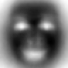
\includegraphics[interpolate=true,width=0.680000in,height=0.680000in]{weights-comparison-img0.png}}%
\end{pgfscope}%
\begin{pgfscope}%
\pgfpathrectangle{\pgfqpoint{0.881364in}{1.680588in}}{\pgfqpoint{0.679412in}{0.679412in}}%
\pgfusepath{clip}%
\pgfsys@transformshift{0.881364in}{1.680588in}%
\pgftext[left,bottom]{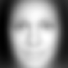
\includegraphics[interpolate=true,width=0.680000in,height=0.680000in]{weights-comparison-img1.png}}%
\end{pgfscope}%
\begin{pgfscope}%
\pgfpathrectangle{\pgfqpoint{0.050000in}{0.865294in}}{\pgfqpoint{0.679412in}{0.679412in}}%
\pgfusepath{clip}%
\pgfsys@transformshift{0.050000in}{0.865294in}%
\pgftext[left,bottom]{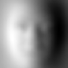
\includegraphics[interpolate=true,width=0.680000in,height=0.680000in]{weights-comparison-img2.png}}%
\end{pgfscope}%
\begin{pgfscope}%
\pgfpathrectangle{\pgfqpoint{0.881364in}{0.865294in}}{\pgfqpoint{0.679412in}{0.679412in}}%
\pgfusepath{clip}%
\pgfsys@transformshift{0.881364in}{0.865294in}%
\pgftext[left,bottom]{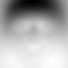
\includegraphics[interpolate=true,width=0.680000in,height=0.680000in]{weights-comparison-img3.png}}%
\end{pgfscope}%
\begin{pgfscope}%
\pgfpathrectangle{\pgfqpoint{0.050000in}{0.050000in}}{\pgfqpoint{0.679412in}{0.679412in}}%
\pgfusepath{clip}%
\pgfsys@transformshift{0.050000in}{0.050000in}%
\pgftext[left,bottom]{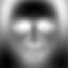
\includegraphics[interpolate=true,width=0.680000in,height=0.680000in]{weights-comparison-img4.png}}%
\end{pgfscope}%
\begin{pgfscope}%
\pgfpathrectangle{\pgfqpoint{0.881364in}{0.050000in}}{\pgfqpoint{0.679412in}{0.679412in}}%
\pgfusepath{clip}%
\pgfsys@transformshift{0.881364in}{0.050000in}%
\pgftext[left,bottom]{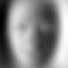
\includegraphics[interpolate=true,width=0.680000in,height=0.680000in]{weights-comparison-img5.png}}%
\end{pgfscope}%
\begin{pgfscope}%
\definecolor{textcolor}{rgb}{0.000000,0.000000,0.000000}%
\pgfsetstrokecolor{textcolor}%
\pgfsetfillcolor{textcolor}%
\pgftext[x=0.780804in,y=2.660000in,,top]{\color{textcolor}\rmfamily\fontsize{12.000000}{14.400000}\selectfont PCA}%
\end{pgfscope}%
\begin{pgfscope}%
\pgfsetbuttcap%
\pgfsetmiterjoin%
\definecolor{currentfill}{rgb}{1.000000,1.000000,1.000000}%
\pgfsetfillcolor{currentfill}%
\pgfsetlinewidth{0.000000pt}%
\definecolor{currentstroke}{rgb}{1.000000,1.000000,1.000000}%
\pgfsetstrokecolor{currentstroke}%
\pgfsetdash{}{0pt}%
\pgfpathmoveto{\pgfqpoint{1.764138in}{-0.280000in}}%
\pgfpathlineto{\pgfqpoint{3.730804in}{-0.280000in}}%
\pgfpathlineto{\pgfqpoint{3.730804in}{2.720000in}}%
\pgfpathlineto{\pgfqpoint{1.764138in}{2.720000in}}%
\pgfpathlineto{\pgfqpoint{1.764138in}{-0.280000in}}%
\pgfpathclose%
\pgfusepath{fill}%
\end{pgfscope}%
\begin{pgfscope}%
\pgfpathrectangle{\pgfqpoint{2.016667in}{1.680588in}}{\pgfqpoint{0.679412in}{0.679412in}}%
\pgfusepath{clip}%
\pgfsys@transformshift{2.016667in}{1.680588in}%
\pgftext[left,bottom]{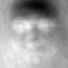
\includegraphics[interpolate=true,width=0.680000in,height=0.680000in]{weights-comparison-img6.png}}%
\end{pgfscope}%
\begin{pgfscope}%
\pgfpathrectangle{\pgfqpoint{2.848030in}{1.680588in}}{\pgfqpoint{0.679412in}{0.679412in}}%
\pgfusepath{clip}%
\pgfsys@transformshift{2.848030in}{1.680588in}%
\pgftext[left,bottom]{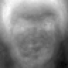
\includegraphics[interpolate=true,width=0.680000in,height=0.680000in]{weights-comparison-img7.png}}%
\end{pgfscope}%
\begin{pgfscope}%
\pgfpathrectangle{\pgfqpoint{2.016667in}{0.865294in}}{\pgfqpoint{0.679412in}{0.679412in}}%
\pgfusepath{clip}%
\pgfsys@transformshift{2.016667in}{0.865294in}%
\pgftext[left,bottom]{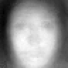
\includegraphics[interpolate=true,width=0.680000in,height=0.680000in]{weights-comparison-img8.png}}%
\end{pgfscope}%
\begin{pgfscope}%
\pgfpathrectangle{\pgfqpoint{2.848030in}{0.865294in}}{\pgfqpoint{0.679412in}{0.679412in}}%
\pgfusepath{clip}%
\pgfsys@transformshift{2.848030in}{0.865294in}%
\pgftext[left,bottom]{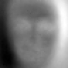
\includegraphics[interpolate=true,width=0.680000in,height=0.680000in]{weights-comparison-img9.png}}%
\end{pgfscope}%
\begin{pgfscope}%
\pgfpathrectangle{\pgfqpoint{2.016667in}{0.050000in}}{\pgfqpoint{0.679412in}{0.679412in}}%
\pgfusepath{clip}%
\pgfsys@transformshift{2.016667in}{0.050000in}%
\pgftext[left,bottom]{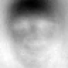
\includegraphics[interpolate=true,width=0.680000in,height=0.680000in]{weights-comparison-img10.png}}%
\end{pgfscope}%
\begin{pgfscope}%
\pgfpathrectangle{\pgfqpoint{2.848030in}{0.050000in}}{\pgfqpoint{0.679412in}{0.679412in}}%
\pgfusepath{clip}%
\pgfsys@transformshift{2.848030in}{0.050000in}%
\pgftext[left,bottom]{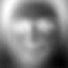
\includegraphics[interpolate=true,width=0.680000in,height=0.680000in]{weights-comparison-img11.png}}%
\end{pgfscope}%
\begin{pgfscope}%
\definecolor{textcolor}{rgb}{0.000000,0.000000,0.000000}%
\pgfsetstrokecolor{textcolor}%
\pgfsetfillcolor{textcolor}%
\pgftext[x=2.747471in,y=2.660000in,,top]{\color{textcolor}\rmfamily\fontsize{12.000000}{14.400000}\selectfont Linear AE}%
\end{pgfscope}%
\begin{pgfscope}%
\pgfsetbuttcap%
\pgfsetmiterjoin%
\definecolor{currentfill}{rgb}{1.000000,1.000000,1.000000}%
\pgfsetfillcolor{currentfill}%
\pgfsetlinewidth{0.000000pt}%
\definecolor{currentstroke}{rgb}{1.000000,1.000000,1.000000}%
\pgfsetstrokecolor{currentstroke}%
\pgfsetdash{}{0pt}%
\pgfpathmoveto{\pgfqpoint{3.730804in}{-0.280000in}}%
\pgfpathlineto{\pgfqpoint{5.697471in}{-0.280000in}}%
\pgfpathlineto{\pgfqpoint{5.697471in}{2.720000in}}%
\pgfpathlineto{\pgfqpoint{3.730804in}{2.720000in}}%
\pgfpathlineto{\pgfqpoint{3.730804in}{-0.280000in}}%
\pgfpathclose%
\pgfusepath{fill}%
\end{pgfscope}%
\begin{pgfscope}%
\pgfpathrectangle{\pgfqpoint{3.983333in}{1.680588in}}{\pgfqpoint{0.679412in}{0.679412in}}%
\pgfusepath{clip}%
\pgfsys@transformshift{3.983333in}{1.680588in}%
\pgftext[left,bottom]{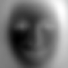
\includegraphics[interpolate=true,width=0.680000in,height=0.680000in]{weights-comparison-img12.png}}%
\end{pgfscope}%
\begin{pgfscope}%
\pgfpathrectangle{\pgfqpoint{4.814697in}{1.680588in}}{\pgfqpoint{0.679412in}{0.679412in}}%
\pgfusepath{clip}%
\pgfsys@transformshift{4.814697in}{1.680588in}%
\pgftext[left,bottom]{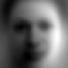
\includegraphics[interpolate=true,width=0.680000in,height=0.680000in]{weights-comparison-img13.png}}%
\end{pgfscope}%
\begin{pgfscope}%
\pgfpathrectangle{\pgfqpoint{3.983333in}{0.865294in}}{\pgfqpoint{0.679412in}{0.679412in}}%
\pgfusepath{clip}%
\pgfsys@transformshift{3.983333in}{0.865294in}%
\pgftext[left,bottom]{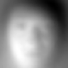
\includegraphics[interpolate=true,width=0.680000in,height=0.680000in]{weights-comparison-img14.png}}%
\end{pgfscope}%
\begin{pgfscope}%
\pgfpathrectangle{\pgfqpoint{4.814697in}{0.865294in}}{\pgfqpoint{0.679412in}{0.679412in}}%
\pgfusepath{clip}%
\pgfsys@transformshift{4.814697in}{0.865294in}%
\pgftext[left,bottom]{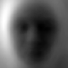
\includegraphics[interpolate=true,width=0.680000in,height=0.680000in]{weights-comparison-img15.png}}%
\end{pgfscope}%
\begin{pgfscope}%
\pgfpathrectangle{\pgfqpoint{3.983333in}{0.050000in}}{\pgfqpoint{0.679412in}{0.679412in}}%
\pgfusepath{clip}%
\pgfsys@transformshift{3.983333in}{0.050000in}%
\pgftext[left,bottom]{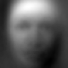
\includegraphics[interpolate=true,width=0.680000in,height=0.680000in]{weights-comparison-img16.png}}%
\end{pgfscope}%
\begin{pgfscope}%
\pgfpathrectangle{\pgfqpoint{4.814697in}{0.050000in}}{\pgfqpoint{0.679412in}{0.679412in}}%
\pgfusepath{clip}%
\pgfsys@transformshift{4.814697in}{0.050000in}%
\pgftext[left,bottom]{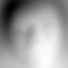
\includegraphics[interpolate=true,width=0.680000in,height=0.680000in]{weights-comparison-img17.png}}%
\end{pgfscope}%
\begin{pgfscope}%
\definecolor{textcolor}{rgb}{0.000000,0.000000,0.000000}%
\pgfsetstrokecolor{textcolor}%
\pgfsetfillcolor{textcolor}%
\pgftext[x=4.714138in,y=2.660000in,,top]{\color{textcolor}\rmfamily\fontsize{12.000000}{14.400000}\selectfont Sigmoid-linear AE}%
\end{pgfscope}%
\end{pgfpicture}%
\makeatother%
\endgroup%

	\caption[Gewichtsmatrizen von ausgewählten Methoden]{Gewichtsmatrizen}
	\label{fig:Gewichtsvergleich}
\end{figure}